% Welcome to the root file for Quantum Microeconomics and Quantum Microeconomics with Calculus! Read on for more information on compiling these documents.



% Last updated: August 2008

%

% Contact: Yoram Bauman, yoram@smallparty.org



% Copyright: All of these documents are covered by Creative Commons Attribution-NonCommercial License. To view a copy of this license, visit Creative Commons online at http://creativecommons.org/licenses/by-nc/3.0/.


% Software requirements: This text was compiled on a PC using MikTeX (free at www.miktex.org) as a LaTeX compiler and WinEdt (not free at www.winedt.com) as a graphical user interface. Any LaTeX compiler with the packages listed below, however, should be able to compile this text; note that the "small" and "medium" MikTeX downloads may not contain all the necessary packages. MikTeX/WinEdt produces a DVI (.dvi) file; I then use WinEdt's "dvips" button to produce a PostScript (.ps) file using Ghostscript (free at http://www.cs.wisc.edu/~ghost/doc/AFPL/get704.htm); this PostScript file can be viewed using Ghostview (free at http://www.cs.wisc.edu/~ghost/gsview/index.htm); finally, I use WinEdt's "ps2pdf" button to produce a PDF (.pdf) file; this PDF file can be viewed using Adobe Acrobat Reader (free at www.abobe.com) and modified using Adobe Acrobat (not free at www.adobe.com).



% Hardware requirements: This text was compiled on a PC, but the hardware should be irrelevant. (Not that I've tested it...)



% Options: There are eight basic options, based on the various combinations of the variables colorlinks, KEY/EXAM, and BASIC/CALCULUS:

% Use "colorlinks=true" in the hyperref package below to create color hyperlinks for online viewing and/or color printing. For black-and-white printing, use "colorlinks=false".

% Use "\excludeversion{KEY}\includeversion{EXAM}" in the version package below to create the text without the answer key. To generate an answer key as an appendix at the end, use "\includeversion{KEY}\excludeversion{EXAM}"; note that this removes the problems from the ends of chapters to avoid multiple references.

% Use "\includeversion{BASIC}\excludeversion{CALCULUS}" for the introductory text Quantum Microeconomics. Use "\excludeversion{BASIC}\includeversion{CALCULUS}" for the intermediate text Quantum Microeconomics with Calculus.
















\documentclass[dvips]{book}
% Note: You may need to change the optional argument [dvips] depending on what you plan to do with the DVI file.

%%%%%%%%%%%\usepackage{endnotes}
%%%%%%%%%%%\let\footnote=\endnote
\usepackage{endnotes} % This whole section comes from Ulrich Diez, http://newsgroups.derkeiler.com/Archive/Comp/comp.text.tex/2007-08/msg00018.html
\makeatletter
\newif\ifenotelinks
\newcounter{Hendnote}
% Redefining portions of endnotes-package:
\let\savedhref\href
\let\savedurl\url
\def\endnotemark{%
\@ifnextchar[\@xendnotemark{%
\stepcounter{endnote}%
\protected@xdef\@theenmark{\theendnote}%
\protected@xdef\@theenvalue{\number\c@endnote}%
\@endnotemark
}%
}%
\def\@xendnotemark[#1]{%
\begingroup\c@endnote#1\relax
\unrestored@protected@xdef\@theenmark{\theendnote}%
\unrestored@protected@xdef\@theenvalue{\number\c@endnote}%
\endgroup
\@endnotemark
}%
\def\endnotetext{%
\@ifnextchar[\@xendnotenext{%
\protected@xdef\@theenmark{\theendnote}%
\protected@xdef\@theenvalue{\number\c@endnote}%
\@endnotetext
}%
}%
\def\@xendnotenext[#1]{%
\begingroup
\c@endnote=#1\relax
\unrestored@protected@xdef\@theenmark{\theendnote}%
\unrestored@protected@xdef\@theenvalue{\number\c@endnote}%
\endgroup
\@endnotetext
}%
\def\endnote{%
\@ifnextchar[\@xendnote{%
\stepcounter{endnote}%
\protected@xdef\@theenmark{\theendnote}%
\protected@xdef\@theenvalue{\number\c@endnote}%
\@endnotemark\@endnotetext
}%
}%
\def\@xendnote[#1]{%
\begingroup
\c@endnote=#1\relax
\unrestored@protected@xdef\@theenmark{\theendnote}%
\unrestored@protected@xdef\@theenvalue{\number\c@endnote}%
\show\@theenvalue
\endgroup
\@endnotemark\@endnotetext
}%
\def\@endnotemark{%
\leavevmode
\ifhmode
\edef\@x@sf{\the\spacefactor}\nobreak
\fi
\ifenotelinks
\expandafter\@firstofone
\else
\expandafter\@gobble
\fi
{%
\Hy@raisedlink{%
\hyper@@anchor{Hendnotepage.\@theenvalue}{\empty}%
}%
}%
\hyper@linkstart{link}{Hendnote.\@theenvalue}%
\makeenmark
\hyper@linkend
\ifhmode
\spacefactor\@x@sf
\fi
\relax
}%
\long\def\@endnotetext#1{%
\if@enotesopen
\else
\@openenotes
\fi
\immediate\write\@enotes{%
\@doanenote{\@theenmark}{\@theenvalue}%
}%
\begingroup
\def\next{#1}%
\newlinechar='40
\immediate\write\@enotes{\meaning\next}%
\endgroup
\immediate\write\@enotes{%
\@endanenote
}%
}%
\def\theendnotes{%
\immediate\closeout\@enotes
\global\@enotesopenfalse
\begingroup
\makeatletter
\edef\@tempa{`\string>}%
\ifnum\catcode\@tempa=12
\let\@ResetGT\relax
\else
\edef\@ResetGT{\noexpand\catcode\@tempa=\the\catcode\@tempa}%
\@makeother\>%
\fi
\def\@doanenote##1##2##3>{%
\def\@theenmark{##1}%
\def\@theenvalue{##2}%
\par
\smallskip %<-small vertical gap between endnotes
\begingroup
\def\href{\expandafter\savedhref}%
\def\url{\expandafter\savedurl}%
\@ResetGT
\edef\@currentlabel{\csname p@endnote\endcsname\@theenmark}%
\enoteformat
}%
\def\@endanenote{%
\par\endgroup
}%
% Redefine, how numbers are formatted in the endnotes-section:
\renewcommand*\@makeenmark{%
\hbox{\normalfont\@theenmark~}%
}%
% header of endnotes-section
\enoteheading
% font-size of endnotes
\enotesize
\input{\jobname.ent}%
\endgroup
}%
\def\enoteformat{%
\rightskip\z@
\leftskip1.8em
\parindent\z@
\leavevmode\llap{%
\setcounter{Hendnote}{\@theenvalue}%
\addtocounter{Hendnote}{-1}%
\refstepcounter{Hendnote}%
\ifenotelinks
\expandafter\@secondoftwo
\else
\expandafter\@firstoftwo
\fi
{\@firstofone}%
{\hyperlink{Hendnotepage.\@theenvalue}}%
{\makeenmark}%
}%
}%
% stop redefining portions of endnotes-package:
\makeatother
% Toggle switch in order to turn on/off back-links in the
% endnote-section:
\enotelinkstrue
%\enotelinksfalse


\usepackage{pstricks, pst-node, pst-tree, pst-plot, pst-text}
% These are Timothy van Zandt's fabulous packages for doing all sort of cool graphics.

\psset{unit=.5cm, levelsep=5cm, labelsep=2pt, tnpos=a, radius=2pt}
% This sets default values for various graphic parameters.

\newpsobject{showgrid}{psgrid}{subgriddiv=1, gridwidth=.5pt, griddots=4, gridlabelcolor=white, gridlabels=0pt}
% This creates gridlines, as used in the supply and demand chapters.



\usepackage[subfigure,AllowH]{graphfig}
%Allows for subfigures, as in the chapter on supply and demand shifts
\renewcommand{\subfigbottomskip}{5pt} % I'm not sure what this command does.


%\def\input@path{{./part0/}{./part1/}{./part2/}{./part3/}{./part4/}}
\graphicspath{{./part0/}{./part1/}{./part2/}{./part3/}{./part4/}}
%This command tells LaTeX to look for graphics files in the subdirectories listed above.



\usepackage{rotating}
% Allows for rotated material



\usepackage{multirow}
% Allows for multiple rows in tables



\renewcommand{\arraystretch}{1.3}
% This is for the payoff matrices, so there's enough space between rows.



\usepackage{ulem}
% This package allows for strike-outs of lines. Usage includes \sout{text} for strike-outs and \xout{text} for cross-outs. See game theory section for examples.
\normalem % This undoes ulem's emph->underline feature so that \emph works properly



\usepackage{mathrsfs}
% This allows us to do Lagrangians
\newcommand{\myl}{\mathscr{L}}
% This defines \myl to be a Lagrangian






% USE THIS COMMAND TO COMPILE ONLY PART OF THE TEXT
%\includeonly{part2/2cake,part2/2pareto}






\definecolor{Myblue}{cmyk}{1,1,0,.3}
\definecolor{Myyellow}{cmyk}{0,0,0,1}%{0,0,1,0}
\definecolor{Mygreen}{cmyk}{0,0,0,1}
%These are for the supply and demand chapters. Defining the colors as (0,0,0,1) makes them all black.




\usepackage{version}
% This package allows for version control, as specified in the arguments below; it also allows you to comment out text using \begin{comment} and \end{comment}.
\includeversion{EXAM}\excludeversion{KEY} % See note above regarding options.
%\includeversion{KEY}\excludeversion{EXAM} % See note above regarding options.
%\includeversion{BASIC}\excludeversion{CALCULUS} % See note above regarding options.
\includeversion{CALCULUS}\excludeversion{BASIC} % See note above regarding options.



\usepackage{makeidx}
\makeindex
% Package and command for making the index; the \printindex command determines where the index prints.






\usepackage[pdfnewwindow=true, colorlinks=true, linkcolor=Myblue, urlcolor=Myblue]{hyperref}
% This package creates hyperlinks. See note above regarding colorlinks options.




%Redefine the first level
\renewcommand{\theenumi}{\arabic{chapter}.\arabic{enumi}}
\renewcommand{\labelenumi}{\theenumi}


\begin{document}



\frontmatter
%See Lamport's text, p. 80; this begins numbering with roman numerals. All sectioning commands except \chapter should appear in *-form.


\begin{BASIC}
\title{Quantum Microeconomics}
%\title{Stand-up Economics:\\ The Micro Textbook}
\author{Version 4.0}% \emph{Beta}}
\end{BASIC}

\begin{CALCULUS}
\title{Quantum Microeconomics\\ \emph{with Calculus}}
%\title{Stand-up Economics:\\ The Micro Textbook\\ \emph{with Calculus}}
\author{Version 4.0}
\end{CALCULUS}

\date{September 2008\\[1in]
Available with and without calculus at\\[.25in] \href{http://www.smallparty.org/yoram/quantum}{http://www.smallparty.org/yoram/quantum}\\[.25in] Email contact: \href{mailto:yoram@smallparty.org}{yoram@smallparty.org}%\\[.25in]
\\[1in]
\begin{center}
\includegraphics*{somerights.eps}
\end{center}
\footnotesize This work is licensed under the Creative Commons Attribution-NonCommercial 3.0 Unported
License. To view a copy of this license, visit Creative Commons online at \href{http://creativecommons.org/licenses/by-nc/3.0/}{http://creativecommons.org/licenses/by-nc/3.0/}.
}
\maketitle



\tableofcontents


%\include{preface} %See LaTeX for everyone to see how to do this \include{pref}, p. 188-190.

%\documentclass{book}
%\begin{document}
%\title{Quantum Microeconomics}
%\author{Yoram Bauman}
%\date{\today}
%\maketitle
%\tableofcontents

\chapter{README.TXT}
\label{intro}
%\addcontentsline{toc}{chapter}{README.TXT}

% Funny, short, story. Maybe Jay Leno's line that anyone can become a successful stand-up comic if they give it seven years.

\begin{quote}
\textbf{quantum }\index{quantum} \textit{Physics.} A minimum amount of a physical quantity which can exist and by multiples of which changes in the quantity occur. (Oxford English Dictionary)
\end{quote}

\vspace*{.4cm}

\noindent The ``quantum" of economics is the optimizing individual. All of economics ultimately boils down to the behavior of such individuals. \textbf{Microeconomics}\index{microeconomics} studies their basic actions and interactions: individual markets, supply and demand, the impact of taxes, monopoly\index{monopoly}, etc. \textbf{Macroeconomics}\index{macroeconomics} then lumps together these individual markets to study national and international issues.

In structure this book---which covers only microeconomics\index{microeconomics}---is not unlike a hiking trip. We start out by putting our boots on and getting our gear together: in Part~\ref{one} we study the optimizing individual. Then we set out on our path and immediately find ourselves hacking through some pretty thick jungle: even simple interactions between just two people (Part~\ref{one_v_one}) can be very complicated! As we add even more people (in studying auctions, for example), things get even more complicated, and the jungle gets even thicker. Then a miracle occurs: we add even more people, and a complex situation suddenly becomes simple. After hacking through thick jungle, we find ourselves in a beautiful clearing: competitive markets (Part~\ref{many_v_many}) are remarkably easy to analyze and understand.

%Part~\ref{one} is the only truly mandatory part of this book, in that later chapters will build on it. For students, this means that understanding the basics from Part~\ref{one} is critical. For instructors, this means that choosing which later chapters to include or not should be fairly painless. The text's modular structure should also provide smooth entry points for other material.

%Many chapters end with supplementary sections dealing with algebra and calculus\index{calculus}; these sections are identified with an italicized \emph{Math}. There are also two supplementary chapters, similarly identified.

\section*{About this book}

My hope is for this book to become a successful \textbf{open source\index{open source}} endeavor \`{a} la the Linux\index{Linux} operating system. You can find out more about open source\index{open source} \href{http://www.opensource.org}{online}\footnote{http://www.opensource.org}; of particular note is Eric S.~Raymond's\index{Raymond, Eric S.} essay ``The Cathedral and the Bazaar", available in bookstores and also \href{http://www.openresources.com/documents/cathedral-bazaar/}{online}\footnote{http://www.openresources.com/documents/cathedral-bazaar/}. % http://tuxedo.org/\~{}esr/writings/cathedral-bazaar/cathedral-bazaar/
Two of the maxims from this essay---which was one of the inspirations for this book---are:
\begin{itemize}
\item If you treat your [users] as if they're your most valuable resource, they will respond by becoming your most valuable resource.
\item (``Linus's Law") Given enough eyeballs, all bugs are shallow.
\end{itemize}
%
Raymond's focus was on software, but I believe that these maxims also hold true for textbooks. In the context of textbooks, ``users" are students and instructors, and ``bugs" are typos, arithmetic mistakes, confusing language, substantive errors, and other shortcomings. (One lesson from \emph{The Cathedral and the Bazaar} is that finding bugs is often harder than fixing them.)

In terms of nuts and bolts, this book is licensed under the Creative Commons  \href{http://creativecommons.org/licenses/by-nc/3.0/}{Attribution-NonCommercial License}\footnote{http://creativecommons.org/licenses/by-nc/3.0/}. The basic idea is that the license allows you to use and/or modify this document for non-commercial purposes as long as you credit \emph{Quantum Microeconomics} as the original source. Combine the legal stuff with the open-source philosophy and here is what it all means\ldots

\smallskip
\noindent\textbf{\ldots For students and instructors}\ \ This book is freely available \href{http://www.smallparty.org/yoram/quantum}{online}\footnote{http://www.smallparty.org/yoram/quantum}. (One advantage of the online edition is that all the ``online'' links are clickable.) Please contribute your comments, suggestions, and ideas for improvement: let me know if you find a typo or a cool website, or even if there's a section of the book that you just found confusing and/or in need of more work. If you're looking for something more substantial to sink your teeth into, you can add or rewrite a section or create some new homework problems. Hopefully you will get some personal satisfaction from your contribution; instructors will hopefully offer extra credit points as well.


\smallskip
\noindent\textbf{\ldots For writers and publishers}\ \ The \LaTeX\ source code for this book--- \LaTeX\index{latex (or \LaTeX)} is a free typesetting program that you can learn about \href{http://www.ctan.org}{online}\footnote{http://www.ctan.org} and/or from many mathematicians or scientists---is available \href{http://www.smallparty.org/yoram/quantum}{online}\footnote{http://www.smallparty.org/yoram/quantum} if you are interested in modifying the text and/or publishing your own version. I encourage you to submit something from your own area of expertise as a contribution to the text: the economic arguments for specialization apply nicely in the world of textbook writing, and the alternative---having one or two people write about such a broad subject---is an invitation for trouble. (For an example, see this excerpt \href{http://www.smallparty.org/yoram/humor/globalwarming.html}{online}\footnote{http://www.smallparty.org/yoram/humor/globalwarming.html}.) 


\section*{Acknowledgments}

The individuals listed below commented on and/or contributed to this text. Thanks to their work, the text is much improved. Please note that listings (which are alphabetical and/or chronological) do not imply endorsement: Melissa Andersen, Kea Asato, Kathryn Bergh, Heather Brandon, Gardner Brown, Katie Chamberlin, Rebecca Charon, Ruth Christiansen, Stacy Fawell, Julie Fields, Aaron Finkle, Jason Gasper, Kevin Grant, Robert Halvorsen, Richard Hartman, Andy Herndon, Rus Higley, Wen Mei Lin, Heather Ludemann, Noelwah Netusil, Anh Nguyen, Elizabeth Petras, Karl Seeley, Amy Seward, Pete Stauffer, Linda Sturgis, Brie van Cleve, Jay Watson.







\begin{comment}


\section*{Revision History and To Do List}

\begin{enumerate}
\item Perpetuities in terms of living off the interest
\item List of figures/tables/jokes
\item Overfull hboxes and vboxes from .log file
\item Glossary
\item Index
\item FCC Auction example
\item Information economics (\textit{Information Rules}, Linux\index{Linux}, Consumer Reports)
\item S\&D together graph is ugly
\item Examples of S\&D shifts
\item Discuss absolute values of elasticities
\end{enumerate}
\end{comment}

\index{differentiation|see{derivative, calculus}}
%\index{uncertainty@uncertainty!see also risk} 
\index{federal government|see{government}}
\index{state government|see{government}}
\index{local government|see{government}} 










\mainmatter
%See Lamport's text, p. 80; this begins numbering with arabic numerals.
\addtocounter{page}{10} %This command makes it so that the PDF page numbering lines up with the text page numbering. If the number of pages in the frontmatter changes, this number will have to change too.

\part{One: The optimizing individual}
\label{one}
%Add chain rule

\chapter{Decision theory}      % Enter chapter title between curly braces
\label{1intro}

\begin{quote}\index{jokes!Zen monk} Two Zen monks walking through a garden stroll onto a small bridge over a goldfish pond and stop to lean their elbows on the railing and look contemplatively down at the fish. One monk turns to the other and says, ``I wish I were a fish; they are so happy and content." The second monk scoffs: ``How do you know fish are happy? You're not a fish!" The reply of the first monk: ``Ah, but how do you know what I know, since you are not me?"
\end{quote}

\vspace*{.4cm}

\noindent Economics is a social science, and as such tries to explain human behavior. Different disciplines---psychology, sociology, political science, anthropology---take different approaches, each with their own strengths and weaknesses; but all try to shed some light on human behavior and (as the joke suggests) all have to make assumptions about how people work. The basic assumption of economics is that \textbf{decisions are made by optimizing individuals}.\index{economics!basic assumption of}

\subsection*{Decisions}

Economics studies the act and implications of choosing. Without choice, there is nothing to study. As Mancur Olson\index{Olson, Mancur} put it in \emph{The Logic of Collective Action}: %(p. 161)
``To say a situation is `lost' or hopeless is in one sense equivalent to saying it is perfect, for in both cases efforts at improvement can bring no positive results."


\subsection*{Individuals}

Economics assumes that the power to make choices resides in the hands of individuals. The approach that economists take in studying the behavior of groups of individuals (consumers, businesses, countries, etc.) is to study the incentives and behaviors of each individual in that group.

The key question in economics is whether---and under what circumstances---\emph{individual} decision-making leads to results that are good \emph{for the group as a whole}. For a pessimistic view on this issue, see the Prisoner's Dilemma game in Chapter~\ref{2simultaneous}. For an optimistic view, see Chapter~\ref{3transition} or consider the words of Adam Smith, who wrote in 1776 that ``[man is] led by an invisible hand\index{invisible hand}\index{hand!invisible} to promote an end which was no part of his intention\ldots. By pursuing his own interest he frequently promotes that of society more effectually than when he really intends to promote it.''


\subsection*{Optimization}

Economics assumes that individuals try to do the best they can. Although economics is unwavering in the assumption that individuals are optimizing---i.e., that each has some objective---there \emph{is} flexibility in determining exactly what those objectives are. In particular, economics does not need to assume that individuals are selfish or greedy; their objectives may well involve friends or family, or people they've never met, or even plants and animals.

Economics also does not make value judgments about different types of individuals; for example, economists do not say that people who avoid risk\index{risk} are better or worse than people who seek out risk\index{risk}. We simply note that, given identical choices, different people act in different ways. In all cases, we assume that each individual is making the decision that is in their best interest.

\smallskip

\noindent \textbf{An aside about individual firms} \ \ Economists often treat companies as optimizing individuals with a goal of \emph{profit maximization\index{profit}.} (For our purposes, \textbf{profit} is simply money in minus money out.\footnote{The ideas in Chapter~\ref{1time} can be used to refine this definition to account for the changing value of money over time. Note also that there are many different definitions of profit, including ``accounting profit"\index{profit!accounting} and ``economic profit"\index{profit!economic}.}) % FIX: Do this is Chapter 1time!
Although the assumption of profit maximization is useful, it does have some problems. One is that some firms---such as food co-operatives---have different goals. A deeper problem is that it is not entirely correct to attribute any goals whatsoever to firms because firms are not optimizing individuals. Rather, a firm is a collection of individuals---workers, managers, stockholders---that is unlikely to function seamlessly as a cohesive optimizing unit because the various individuals have their own objectives. While some branches of economics do analyze the goings-on inside firms, in many cases it is valuable to simplify matters by assuming---as we will throughout this book---that firms act like optimizing individuals and that their objective is to maximize profit\index{profit}.

\smallskip

\noindent \textbf{An aside about individual people} \ \ Economists say that optimizing individuals pursue \emph{utility maximization}. Although you can think of \textbf{utility} as simply a fancy word for happiness, some complex philosophical and mathematical ideas lie under the surface. At the heart of modern economic theory is the idea of \emph{preferences}: given two options, an individual can say that she prefers one over the other (or that she likes them both equally). If we make certain assumptions---e.g., that if the individual prefers A over B and prefers B over C then she prefers A over C---then we can represent individual preferences using a \textbf{utility function} that assigns a number (a ``happiness level") to each option. Economists in the late 1900s thought that utility might actually be real, something that could be measured using ``hedonometers" or ``psychogalvanometers". In contrast, modern economic theory treats utility as simply a handy mathematical technique for representing an individual's preferences: saying that option A produces a utility of 20 and option B produces a utility of 10 means no more and no less than saying that the individual prefers A to B.\footnote{For details, see Jean-Jacques Laffont, \emph{The Economics of Uncertainty and Information} (MIT Press, 1995), or Mas-Colell, Whinston, and Green, \emph{Microeconomic Theory} (Oxford Univ.\ Press, 1995), which is basically the \emph{Joy of Cooking} of microeconomics.}


\section{Decision trees\index{decision tree}}       % Choices in Boxes or Decision Theory???

%\enlargethispage{\baselineskip} % This and the one below are to squeeze this chapter onto one less page.

We can imagine that optimizing individuals make decisions by listing all the options and then choosing the best one. We can visualize this process with the help of a \textbf{decision tree\index{decision tree}} (Figure~\ref{fig:dtree_basic}). The individual starts at the left-most node on the tree, chooses between the various options, and continues moving along the branches until he reaches one of the payoff boxes at the end of the tree.

\begin{Figure}[h]{A simple decision tree\index{decision tree}}[fig:dtree_basic]
\begin{pspicture}(-4,-4)(16,4)
\psset{levelsep=3cm}
\pstree[treemode=R]{\TC*}
{
\TC*~[tnpos=r]{\psframebox{$\displaystyle\frac{\mbox{Outcome 1}}{\ldots}$}}
%\taput{Option 1}
\pstree{\TC*}
{\TC*~[tnpos=r]{\psframebox{$\displaystyle\frac{\mbox{Outcome 2}}{\ldots}$}}
\TC*~[tnpos=r]{\psframebox{$\displaystyle\frac{\mbox{Outcome 3}}{\ldots}$}}
}
}
\end{pspicture}
\end{Figure}

% FIX: PUT IN EXAMPLE??? Car Mechanic?

%This type of systematic analysis can be quite important, as can be seen in the ``Calculating Your Real Hourly Wage" excerpt from \emph{Your Money or Your Life} in the reading packet.

Comparing the items in the various payoff boxes, we can see that some are in all the payoff boxes and some are not. Items that are in all the payoff boxes are called \textbf{sunk costs\index{cost!sunk}}. For example, say you pay \$20 to enter an all-you-can-eat restaurant. Once you enter and begin making choices about what to eat, the \$20 you paid to get into the restaurant becomes a sunk cost: no matter what you order, you will have paid the \$20 entrance fee.

The important thing about sunk costs\index{cost!sunk} is that they're often not important. \emph{If the same item is in all of the payoff boxes, it's impossible to make a decision solely on the basis of that item.} Sunk costs\index{cost!sunk} can provide important background material for making a decision (see problem~\ref{sunkcostmatters}), but the decision-making process depends crucially on items that are not in all the boxes.

Once you think you've found the best choice, a good way to check your work is to look at some nearby choices. Such \textbf{marginal analysis\index{marginal!analysis}} basically involves asking ``Are you sure you don't want a little more or a little less?" For example, imagine that an optimizing individual goes to the grocery store, sees that oranges are 25 cents apiece (i.e., that the \textbf{marginal cost\index{marginal!cost}} of each orange is 25 cents), and decides to buy five. One nearby choice is ``Buy four"; since our optimizing individual chose ``Buy five" instead, her \textbf{marginal benefit\index{marginal!benefit}} from the fifth orange must be \emph{more} than 25 cents. Another nearby choice is ``Buy six''; since our optimizing individual chose ``Buy five'' instead,  her marginal benefit\index{marginal!benefit} from a sixth orange must be \emph{less} than 25 cents.

%FIX: Do example with firm.

As an analogy for marginal analysis, consider the task of finding the highest place on Earth. If you think you've found the highest place, marginal analysis helps you verify this by establishing a condition that is \emph{necessary but not sufficient}: in order for some spot to be the highest spot on Earth, it is necessarily true that moving a little bit in any direction cannot take you any higher. Simple though it is, this principle is quite useful for checking your work. (It is not, however, infallible: although all mountain peaks pass the marginal analysis test, not all of them rank as the highest spot on Earth.)


\section{Example: Monopoly}

Recall that one of our assumptions is that firms are profit-maximizing. This assumption takes on extra significance in the case of \textbf{monopoly\index{monopoly}}---i.e., when there is only one seller of a good---because of the lack of competition. We will see in Part~\ref{many_v_many} that competition between firms imposes tight constraints on their behavior. In contrast, monopolists have more freedom, and a key component of that freedom is the ability to set whatever price they want for their product.\footnote{For this reason, firms with monopoly power are also known as \textbf{price-setting} firms, whereas firms in a competitive market are known as \textbf{price-taking} firms.} Indeed, we will see in Part~\ref{one_v_one} that monopolists will try to charge different people different prices based on their willingness to pay for the product in question.

For now, however, we will focus on a \textbf{uniform pricing monopolist}---like the one in Figure~\ref{fig:dtree_monopoly}---who must charge all customers the same price. In this situation, the monopolist's profit is calculated according to
\begin{eqnarray*}
\mbox{Profit} & = & \mbox{Total Revenue} - \mbox{Total Costs} \\
& = & \mbox{Price} \cdot \mbox{Quantity} - \mbox{Total Costs}
\end{eqnarray*}
% FIX: Halvorsen said something about how this is the definition of profit, not the profit function. I think he thinks the profit function is pq - c(q) or something.
From this equation we can see that a profit-maximizing monopolist will try to minimize costs, just like any other firm; every dollar they save in costs is one more dollar of profit. So the idea that monopolists are slow and lazy doesn't find much support in this model.\footnote{More progress can be made in this direction by studying \textbf{regulated monopolies}\index{monopoly!regulated} that are guaranteed a certain profit level by the government. Such firms are not always allowed to keep cost savings that they find.}%, and they often have a \textbf{cost-plus} agreement that ensures that they will receive sufficient revenue to cover their costs plus earn some predetermined profit. In these cases there can be substantial incentives for \textbf{gold-plating}, e.g., building fancy office buildings with gold-plated bathroom fixtures. }
% FIX: Halvorsen really didn't like this footnote. He says that cost-plus monopolies will still minimize costs (with some conditions, I think, e.g., that demand is elastic or something). Work on this!

%Second, we can catch a glimpse of the monopolist's fundamental problem: it faces a trade-off between \textbf{profit margin} (making a lot of money on each unit by charging a high price) and \textbf{volume} (making a lot of money by selling lots of units). The decision tree in Figure~\ref{fig:dtree_monopoly} shows some of the different price options for a hypothetical monopolist; it also shows that a higher price will drive away customers, thereby reducing the quantity that it sells. (This inverse relationship between price and the quantity that customers want to buy is formally known as the \textbf{Law of Demand}.) The monopolist would like to sell a large quantity for a high price, but it is forced to choose between selling a smaller quantity for a high price and selling a larger quantity for a low price. The decision tree shows that the monopolist's optimal choice in this example is to choose a price of \$5 per unit.


\begin{Figure}[p]{A decision tree\index{decision tree} for a uniform-pricing monopoly. The second line in each payoff box shows the amount that buyers are willing to buy at the given price. The third line show the monopolist's total revenue if it chooses the given price; note that the highest price (\$6 per unit) yields \emph{less} revenue than lower prices! The fourth line shows the monopolist's costs for producing the amount that buyers want to buy at the given price; in this case there are constant production costs of \$1 per unit. The final line shows the monopolist's profit, identifying a price of \$5 per unit as the profit-maximizing choice.}[fig:dtree_monopoly]
\begin{pspicture}(-1,-14.5)(16,14.5)
\psset{levelsep=5cm}
\pstree[treemode=R]{\TC*}
{
\TC*~[tnpos=r]{\fbox{\parbox{6cm}{\textbf{At a price of \$2 per unit:}\\buyers will buy 7 million units;\\total revenue will be $2\cdot 7=\$14$ million;\\total cost will be \$7 million; and \\profit will be $14-7=\$7$ million}}}
\TC*~[tnpos=r]{\fbox{\parbox{6cm}{\textbf{At a price of \$3 per unit:}\\buyers will buy 6 million units;\\total revenue will be $3\cdot 6=\$18$ million;\\total cost will be \$6 million; and \\profit will be $18-6=\$12$ million}}}
\TC*~[tnpos=r]{\fbox{\parbox{6cm}{\textbf{At a price of \$4 per unit:}\\buyers will buy 5 million units;\\total revenue will be $4\cdot 5=\$20$ million;\\total cost will be \$5 million; and \\profit will be $20-5=\$15$ million}}}
\TC*~[tnpos=r]{\fbox{\parbox{6cm}{\textbf{At a price of \$5 per unit:}\\buyers will buy 4 million units;\\total revenue will be $5\cdot 4=\$20$ million;\\total cost will be \$4 million; and \\profit will be $20-4=\$16$ million}}}
\TC*~[tnpos=r]{\fbox{\parbox{6cm}{\textbf{At a price of \$6 per unit:}\\buyers will buy 3 million units;\\total revenue will be $6\cdot 3=\$18$ million;\\total cost will be \$3 million; and \\profit will be $18-3=\$15$ million}}}
}
\end{pspicture}
% This is c(q)=q, q=9-p, with q measured in $millions.
\end{Figure}


We can also see the monopolist's \textbf{uniform pricing problem}: it would like to sell a large quantity for a high price, but it is forced to choose between selling a smaller quantity for a high price and selling a larger quantity for a low price. In other words, it faces a trade-off between \textbf{profit margin} (making a lot of money on each unit by charging a high price) and \textbf{volume} (making a lot of money by selling lots of units). The decision tree in Figure~\ref{fig:dtree_monopoly} gives an example showing how a higher price will drive away customers, thereby reducing the quantity that the monopolist can sell. In Part~\ref{many_v_many} we will return to the inverse relationship between price and the quantity that customers want to buy, a relationship formally known as the \textbf{Law of Demand}.



%\footnote{If you do calculus\index{calculus}: the mathematics of optimization simply involves taking derivatives and setting them equal to zero. This is precisely what marginal analysis\index{marginal!analysis} entails: you look at small changes (e.g., $\Delta x$) and then take limits as $\Delta x$ approaches zero. Since we don't do calculus\index{calculus} here, we stop at $\Delta x$.}

\begin{CALCULUS}

\section{\emph{Math}: Optimization and calculus\index{calculus}}


\subsection*{Derivatives in theory}

The \textbf{derivative\index{derivative}} of a function $f(x)$, written $\displaystyle \frac{d}{dx}\left[ f(x)\right]$ or $\displaystyle \frac{d\,  f(x)}{dx}$ or $f'(x)$, measures the \emph{instantaneous rate of change} of $f(x)$:
\[
\frac{d}{dx}\left[ f(x)\right] = \lim_{h\rightarrow 0} \frac{f(x+h) - f(x)}{h}.
\]
%
Intuitively, derivatives measures \textbf{slope\index{slope!and derivative}}: $f'(x)=-3$ intuitively means that if $x$ increases by $1$ then $f(x)$ will decrease by $3$. This intuition matches up with setting $h=1$, which yields
\[
f'(x)\approx \frac{f(x+1)-f(x)}{1} = f(x+1)-f(x).
\]

All of the functions we use in this class have derivatives (i.e., are \textbf{differentiable}), which intuitively means that they are smooth and don't have kinks or discontinuities. The maximum and minimum values of such functions must either be \textbf{corner solutions}---such as $x=\infty$, $x=-\infty$, or (if we are trying to maximize $f(x)$ subject to $x\geq x_{min}$) $x=x_{min}$---or \textbf{interior solutions\index{interior solution}}. The vast majority of the problems in this class will have interior solutions\index{interior solution}.

At an interior maximum or minimum, the slope\index{slope!and derivative} $f'(x)$ must be zero. Why? Well, if $f'(x)\neq 0$ then either $f'(x)>0$ or $f'(x)<0$. Intuitively, this means that you're on the side of a hill---if $f'(x)>0$ you're going uphill, if $f'(x)<0$ you're heading downhill---and if you're on the side of a hill then you're not at the top (a maximum) or at the bottom (a minimum). At the top and the bottom the slope\index{slope!and derivative} $f'(x)$ will be zero.

To say the same thing in math: If $f'(x)\neq 0$ then either $f'(x)>0$ or $f'(x)<0$. If $f'(x)>0$ then $f(x+h)>f(x)$ (this comes from the definition of derivative), so $f(x)$ isn't a maximum; and $f(x-h)<f(x)$ (this follows from continuity, i.e., the fact that $f(x)$ is a smooth function), so $f(x)$ isn't a minimum. Similarly, if $f'(x)<0$ then $f(x+h)<f(x)$ (this comes from the definition of derivative), so $f(x)$ isn't a minimum; and $f(x-h)>f(x)$ (this follows from continuity), so $f(x)$ isn't a maximum. So the only possible (interior) maxima or minima must satisfy $f'(x)=0$, which is called a \textbf{necessary first-order condition\index{necessary first-order condition}}.

\bigskip

\noindent \emph{In sum: to find candidate values for (interior) maxima or minima, simply take a derivative and set it equal to zero, i.e., find values of $x$ that satisfy $f'(x)=0$.}

\bigskip

Such values do not \emph{have} to be maxima or minima: the condition $f'(x)=0$ is \emph{necessary} but not \emph{sufficient}. This is a more advanced topic that we will not get into in this course, but for an example consider $f(x)=x^3$. Setting the derivative ($3x^2$) equal to zero has only one solution: $x=0$. But $x=0$ is neither a minimum nor a maximum value of $f(x)=x^3$. The \textbf{sufficient second-order condition\index{sufficient second-order condition}} has to do with the second derivative (i.e., the derivative of the derivative, written $f''(x)$). For a maximum, the sufficient second-order condition\index{sufficient second-order condition} is $f''(x)<0$; this guarantees that we're on a hill, so together with $f'(x)=0$ it guarantees that we're on the top of the hill.  For a minimum, the sufficient second-order condition\index{sufficient second-order condition} is $f''(x)>0$; this guarantees that we're in a valley, so together with $f'(x)=0$ it guarantees that we're at the bottom of the valley.)

\subsubsection*{Partial derivatives\index{derivative!partial}}

For functions of two or more variables such as $f(x,y)$, it is often useful to see what happens when we change one variable (say, $x$) without changing the other variables. (For example, what happens if we walk in the north-south direction without changing our east-west position?) What we end up with is the \emph{partial derivative with respect to $x$} of the function $f(x,y)$, written $\displaystyle \frac{\partial}{\partial x}\left[ f(x,y)\right]$ or $f_x(x,y)$:
\[
\frac{\partial}{\partial x}\left[ f(x,y)\right] = \lim_{h\rightarrow 0} \frac{f(x+h, y) - f(x,y)}{h}.
\]
%
Partial derivatives measure rates of change or slopes\index{slope!and partial derivative} \emph{in a given direction}: $f_x(x,y)=3y$ intuitively means that if $x$ increases by $1$ and $y$ doesn't change then $f(x,y)$ will increase by $3y$. Note that ``regular" derivatives and partial derivatives mean the same thing for a function of only one variable: $\displaystyle \frac{d}{dx}[f(x)] = \frac{\partial}{\partial x}[f(x)]$.

At an (interior) maximum or minimum of a smooth function, the slope\index{slope!and partial derivative} must be zero \emph{in all directions}. In other words, the necessary first-order conditions\index{necessary first-order condition} are that \emph{all} partials must be zero: $f_x(x,y)=0$, $f_y(x,y)=0$, etc. Why? For the same reasons we gave before: if one of the partials---say, $f_y(x,y)$---is not zero, then moving in the $y$ direction takes us up or down the side of a hill, and so we cannot be at a maximum or minimum value of the function $f(x,y)$.

\bigskip

\noindent \emph{In sum: to find candidate values for (interior) maxima or minima, simply take partial derivatives with respect to all the variables and set them equal to zero, e.g., find values of $x$ and $y$ that simultaneously satisfy $f_x(x,y)=0$ \emph{and} $f_y(x,y)=0$.}

\bigskip

As before, these conditions are necessary but not sufficient. This is an even more advanced topic than before, and we will not get into it in this course; all I will tell you here is that (1) the sufficient conditions for a maximum include $f_{xx}<0$ and $f_{yy}<0$, \emph{but these aren't enough}, (2) you can find the sufficient conditions in most advanced textbooks, e.g., Silberberg\index{Silberberg, Eugene} and Suen's\index{Suen, Wing} \emph{The Structure of Economics}, and (3) an interesting example to consider is $\displaystyle f(x,y)=\frac{\cos(x)}{\cos(y)}$ around the point $(0,0)$.

%\clearpage

One final point: Single variable derivatives can be thought of as a degenerate case of partial derivatives: there is no reason we can't write $f_x(x)$ instead of $f'(x)$ or $\displaystyle \frac{\partial}{\partial x} f(x)$ instead of $\displaystyle \frac{d}{dx} f(x)$. All of these terms measure the same thing: the rate of change of the function $f(x)$ in the $x$ direction.




\subsection*{Derivatives in practice}

To see how to calculate derivatives, let's start out with a very simple function: the constant function $f(x)=c$, e.g., $f(x)=2$. We can calculate the derivative of this function from the definition:
\[
\frac{d}{dx}(c) = \lim_{h\rightarrow 0} \frac{f(x+h) - f(x)}{h} = \lim_{h\rightarrow 0} \frac{c - c}{h} =0.
\]
So the derivative of $f(x)=c$ is $\displaystyle \frac{d}{dx}(c) = 0$. Note that \emph{all} values of $x$ are candidate values for maxima and/or minima. Can you see why?\footnote{Answer: All values of $x$ \emph{are} maxima; all values are minima, too! Any $x$ you pick gives you $f(x)=c$, which is both the best and the worst you can get.}

Another simple function is $f(x)=x$. Again, we can calculate the derivative from the definition:
\[
\frac{d}{dx}(x) = \lim_{h\rightarrow 0} \frac{f(x+h) - f(x)}{h} = \lim_{h\rightarrow 0} \frac{(x+h) - x}{h} =\lim_{h\rightarrow 0} \frac{h}{h}=1.
\]
So the derivative of $f(x)=x$ is $\displaystyle \frac{d}{dx} (x) = 1$. Note that \emph{no} values of the function $f(x)=x$ are candidate values for maxima or minima. Can you see why?\footnote{Answer: There are no interior maxima or minima of the function $f(x)=x$.}

A final simple derivative involves the function $g(x) = c\cdot f(x)$ where $c$ is a constant and $f(x)$ is any function:
\[
\frac{d}{dx}[c\cdot f(x)] = \lim_{h\rightarrow 0} \frac{c\cdot f(x+h) - c\cdot f(x)}{h} = c\cdot \lim_{h\rightarrow 0} \frac{f(x+h) - f(x)}{h}.
\]
The last term on the right hand side is simply the derivative of $f(x)$, so the derivative of $g(x) = c\cdot f(x)$ is
$\displaystyle \frac{d}{dx}[c\cdot f(x)] = c\cdot \frac{d}{dx}[f(x)]$.






\subsubsection*{More complicated derivatives}

To differentiate (i.e., calculate the derivative of) a more complicated function, use various differentiation rules to methodically break down your problem until you get an expression involving the derivatives of the simple functions shown above.

The most common rules are those involving the three main binary operations: addition, multiplication, and exponentiation.
\begin{itemize}
\item \textbf{Addition}\ \ \ $\displaystyle \frac{d}{dx} \left[
f(x) + g(x) \right]  = \frac{d}{dx} \left[ f(x) \right] +
\frac{d}{dx} \left[ g(x) \right]$.

\medskip

Example: $\displaystyle \frac{d}{dx} \left[ x + 2 \right]  =
\frac{d}{dx} \left[ x \right] + \frac{d}{dx} \left[ 2 \right] = 1
+ 0 = 1.$

Example: $\displaystyle \frac{d}{dx} \left[ 3x^2(x+2) + 2x \right]
= \frac{d}{dx} \left[ 3x^2(x+2) \right] + \frac{d}{dx} \left[ 2x
\right].$

\medskip

\item \textbf{Multiplication}\ \ \  $\displaystyle \frac{d}{dx}
\left[ f(x)\cdot g(x) \right]  =  f(x)\cdot \frac{d}{dx} \left[
g(x) \right] + g(x) \cdot \frac{d}{dx} \left[ f(x) \right].$

\medskip

Example: $\displaystyle \frac{d}{dx} \left[ 3x \right]  =  3\cdot
\frac{d}{dx} \left[ x \right] + x \cdot \frac{d}{dx} \left[ 3
\right] = 3(1) + x(0) = 3.$

(Note: this also follows from the result that $\displaystyle
\frac{d}{dx}[c\cdot f(x)] = c\cdot \frac{d}{dx}[ f(x)]$.)

Example: $\displaystyle \frac{d}{dx} \left[ x(x+2) \right]  =
x\cdot \frac{d}{dx} \left[ (x+2) \right] + (x+2) \cdot
\frac{d}{dx} \left[ x \right] = 2x+2.$

Example: $\displaystyle \frac{d}{dx} \left[ 3x^2(x+2) \right]  =
3x^2\cdot \frac{d}{dx} \left[ (x+2) \right] + (x+2) \cdot
\frac{d}{dx} \left[ 3x^2 \right].$

\medskip

\item \textbf{Exponentiation} \ \ \  $\displaystyle
\frac{d}{dx}\left[ f(x)^a \right]  =  a\cdot f(x)^{a-1} \cdot
\frac{d}{dx}\left[f(x)\right].$

\medskip

Example: $\displaystyle \frac{d}{dx}\left[ (x+2)^2 \right]  =
2(x+2)^1\cdot \frac{d}{dx}\left[x+2 \right] = 2(x+2)(1) = 2(x+2).$

Example: $\displaystyle \frac{d}{dx}\left[ (2x+2)^{\frac{1}{2}}
\right]  =  \frac{1}{2}(2x+2)^{-\frac{1}{2}}\cdot
\frac{d}{dx}\left[2x+2 \right] = (2x+2)^{-\frac{1}{2}}.$

\medskip

\end{itemize}

\noindent Putting all these together, we can calculate lots of messy derivatives:
\begin{eqnarray*}
\frac{d}{dx} \left[ 3x^2(x+2) + 2x \right]  & = & \frac{d}{dx} \left[ 3x^2(x+2) \right] + \frac{d}{dx} \left[ 2x \right]\\
& = & 3x^2\cdot \frac{d}{dx} \left[ x+2\right] + (x+2) \cdot \frac{d}{dx} \left[ 3x^2 \right] + \frac{d}{dx} \left[ 2x \right]\\
& = & 3x^2(1) + (x+2)(6x) + 2\\
& = & 9x^2+12x+2
\end{eqnarray*}


\subsubsection*{Subtraction and division}

The rule for addition also works for subtraction, and can be seen by treating $f(x)-g(x)$ as $f(x)+ (-1)\cdot g(x)$ and using the rules for addition and multiplication. Less obviously, the rule for multiplication takes care of division: $\displaystyle \frac{d}{dx} \left[ \frac{f(x)}{g(x)} \right] = \frac{d}{dx} \left[ f(x)\cdot g(x)^{-1} \right]$. Applying the product and exponentiation rules to this yields the quotient rule,\footnote{Popularly remembered as  $\displaystyle \ d \left[\frac{\mbox{Hi}}{\mbox{Ho}} \right] = \frac{\mbox{Ho}\cdot d\mbox{Hi} - \mbox{Hi}\cdot d\mbox{Ho}}{\mbox{Ho}\cdot\mbox{Ho}}.$}
%
\begin{itemize}

\medskip

\item \textbf{Division}\ \ \  $\displaystyle
\frac{d}{dx}\left[\frac{f(x)}{g(x)} \right] =
\frac{g(x)\cdot\frac{d}{dx}f(x) -
f(x)\cdot\frac{d}{dx}g(x)}{\left[ g(x)\right]^2}.$

\medskip

Example: $\displaystyle \frac{d}{dx}\left[\frac{3x^2+2}{-e^x}
\right] = \frac{-e^2\cdot\frac{d}{dx}[3x^2+2] -
(3x^2+2)\cdot\frac{d}{dx}[-e^x]}{\left[ -e^x\right]^2}.$
\end{itemize}

\subsubsection*{Exponents}

If you're confused about what's going on with the quotient rule, you may find value in the following rules about exponents, which we will use frequently:

\begin{center}
\begin{tabular}{cccc}
$x^a\cdot x^b = x^{a+b}$\hspace{.7cm} & $\left(x^a\right)^b =
x^{ab}$\hspace{.7cm} & $\displaystyle x^{-a} = \frac{1}{x^a}$
\hspace{.7cm} & $\displaystyle (xy)^a = x^a y^a$\hspace{.7cm}
\end{tabular}
\end{center}

\noindent Examples: $2^2 \cdot 2^3 = 2^5$,\ \ $(2^2)^3 = 2^6$, \ \
$2^{-2}=\frac{1}{4}$,\ \  $(2\cdot 3)^2 = 2^2\cdot 3^2$.


\subsubsection*{Other differentiation rules: $e^x$ and $\ln (x)$}

You won't need the chain rule, but you may need the rules for derivatives involving the exponential function $e^x$ and the natural logarithm function $\ln(x)$. (Recall that $e$ and $\ln$ are inverses of each other, so that $\displaystyle e^{(\ln x)} = \ln (e^x) = x$.)


\begin{itemize}
\item \textbf{The exponential function}\ \ \  $\displaystyle
\frac{d}{dx}\left[ e^{f(x)} \right] = e^{f(x)}\cdot
\frac{d}{dx}\left[ f(x)\right].$

\medskip

Example: $\displaystyle \frac{d}{dx}\left[ e^x \right] = e^x\cdot
\frac{d}{dx}\left[ x\right] = e^x.$

Example: $\displaystyle \frac{d}{dx}\left[ e^{3x^2+2} \right] =
e^{3x^2+2}\cdot \frac{d}{dx}\left[ 3x^2+2\right] =
e^{3x^2+2}\cdot(6x).$

\medskip

\item \textbf{The natural logarithm function} \ \ \ $\displaystyle
\frac{d}{dx}\left[ \ln f(x) \right] =
\frac{1}{f(x)}\cdot\frac{d}{dx}\left[f(x)\right].$

\medskip
Example: $\displaystyle \frac{d}{dx}\left[ \ln x \right] =
\frac{1}{x}\cdot\frac{d}{dx}\left[x\right] = \frac{1}{x}.$

Example: $\displaystyle \frac{d}{dx}\left[ \ln (3x^2+2) \right] =
\frac{1}{3x^2+2}\cdot\frac{d}{dx}\left[3x^2+2\right] =
\frac{1}{3x^2+2}(6x).$

\end{itemize}


\subsection*{Partial derivatives}

Calculating partial derivatives (say, with respect to $x$) is easy: just treat all the other variables as constants while applying all of the rules from above. So, for example,
\begin{eqnarray*}
\frac{\partial}{\partial x}\left[ 3x^2y + 2e^{xy}-2y\right] & = & \frac{\partial}{\partial x}\left[ 3x^2y \right] + \frac{\partial}{\partial x}\left[ 2e^{xy} \right] -  \frac{\partial}{\partial x}\left[ 2y\right]\\
& = & 3y\frac{\partial}{\partial x}\left[ x^2 \right] + 2e^{xy}\frac{\partial}{\partial x}\left[ xy \right] -  0 \\
& = & 6xy + 2ye^{xy}.
\end{eqnarray*}
Note that the partial derivative $f_x(x,y)$ is a function of both $x$ \emph{and} $y$. This simply says that the rate of change with respect to $x$ of the function $f(x,y)$ depends on where you are in both the $x$ direction and the $y$ direction.

We can also take a partial derivative with respect to $y$ of the
same function:
\begin{eqnarray*}
\frac{\partial}{\partial y}\left[ 3x^2y + 2e^{xy}-2y\right] & = & \frac{\partial}{\partial y}\left[ 3x^2y \right] + \frac{\partial}{\partial y}\left[ 2e^{xy} \right] -  \frac{\partial}{\partial y}\left[ 2y\right]\\
& = & 3x^2\frac{\partial}{\partial y}\left[ y \right] + 2e^{xy}\frac{\partial}{\partial y}\left[ xy \right] -  2 \\
& = & 3x^2 + 2xe^{xy} - 2.
\end{eqnarray*}
Again, this partial derivative is a function of both $x$ and $y$.


\subsection*{Integration\index{integrals}}

The integral of a function, written $\int_a^b f(x)\, dx$, measures the \emph{area} under the function $f(x)$ between the points $a$ and $b$. We won't use integrals much, but they are related to derivatives by the Fundamental Theorem(s) of Calculus\index{calculus}:

\begin{center}
\begin{tabular}{cc}
$\displaystyle \int_a^b \frac{d}{dx}\left[ f(x)\right]\, dx  =
f(b) - f(a)$\ \ \ \ \ \  & $\displaystyle \frac{d}{ds}\left[
\int_a^s f(x)\, dx \right] = f(s)\ \ \ \ \ \ $
\end{tabular}
\end{center}

\noindent Example: $\displaystyle \int_0^1 x \, dx= \int_0^1
\frac{d}{dx}\left[ \frac{1}{2}x^2\right]\, dx  = \frac{1}{2}(1^2)
- \frac{1}{2}(0^2) = \frac{1}{2}$

\medskip

\noindent Example: $\displaystyle \frac{d}{ds}\left[ \int_0^s x\,
dx \right] = s.$

\end{CALCULUS}



%\bigskip
%\bigskip
%\begin{BASIC}
%\clearpage
%\end{BASIC}
\section*{Problems}

\noindent \textbf{Answers are in the endnotes beginning on page~\pageref{1introa}. If you're reading this online, click on the endnote number to navigate back and forth.}


\begin{enumerate}


\item\index{cost!sunk} A newspaper column in the summer of 2000 complained about the overwhelming number of hours being devoted to the Olympics by NBC. The columnist argued that NBC had such an extensive programming schedule in order to recoup the millions of dollars it had paid for the rights to televise the games. Do you believe this argument? Why or why not?%s
\endnote{\label{1introa}You should not believe this argument because the amount spent on the rights to the Olympic Games is a sunk cost. The reason the network showed the Olympics for so many hours was because that was the decision that maximized profits.

\begin{CALCULUS}
We can also see this mathematically: the amount spent on the rights to the Games is a constant term in the profit function, e.g., $\pi = f(h) - c$ where $f(h)$ are advertising revenues from showing the games for $h$ hours and $c$ is the amount spent on the rights to the games. To maximize this, we take a derivative with respect to $h$ and set it equal to zero. Note that the constant term $c$ drops out when we take a derivative, and therefore has no impact on the optimal choice of $h$.
\end{CALCULUS}
}



\item\label{sunkcostmatters}\index{cost!sunk} You win \$1 million in the lottery, and the lottery officials offer you the following bet: You flip a coin; if it comes up heads, you win an additional \$10 million; if it comes up tails, you lose the \$1 million. Will the amount of money you had prior to the lottery affect your decision? (\emph{Hint:} What would you do if you were already a billionaire? What if you were penniless?) What does this say about the importance of sunk costs?%
\endnote{A billionaire would probably take this bet because this is a terrific (although risky) investment. A penniless person would probably not take the bet because the risk of ending up with zero is too great. So sunk costs cannot be entirely ignored in decision-making; rather, the point is that it is not possible to base decisions \emph{solely} on sunk costs.
}

%\enlargethispage{\baselineskip} % This and the one above are to squeeze this chapter onto one less page.

\item Alice the axe murderer is on the FBI's Ten Most Wanted list for killing six people. If she is caught, she will be convicted of these murders. The government decides to get tough on crime by passing a new law saying that anybody convicted of murder will get the death penalty. Does this serve as a deterrent for Alice, i.e., does the law give Alice an incentive to stop killing people? Does the law serve as a deterrent for Betty, who is thinking about becoming an axe murderer but hasn't killed anybody yet?%(\emph{Hint:} ``\,`In light of the fact that Texas executes more prisoners than any other state, we have to recognize how vulnerable we are,' said Dennis Longmire, a criminal justice professor at Sam Houston State University in Huntsville. `These men really have nothing to lose.'" Michelle Koidin, ``Gang of Inmates Hunted in Slaying", \emph{Hartford Courant}, Dec. 27, 2000.)
\endnote{The law does not deter Alice from committing additional crimes because she's already facing the death penalty if she's caught. The law does deter Betty, because she hasn't killed anybody yet.
}




\item \index{cost!sunk} A drug company comes out with a new pill that prevents baldness. When asked why the drug costs so much, the company spokesman says that they needs to recoup the \$1 billion spent on research and development (R\&D).

\begin{enumerate}

\item Will a profit-maximizing firm pay attention to R\&D costs when determining its pricing?

\item If you said ``Yes" above: Do you think the company would have charged less for the drug if it had discovered it after spending only \$5 million instead of \$1 billion?

If you said ``No" above: Do R\&D costs affect the company's behavior (1) \emph{before} they decide whether or not to invest in the R\&D, (2) \emph{after} they invest in the R\&D, (3) both before and after, or (4) neither?%
\endnote{You should not believe the spokesman's explanation because the R\&D expenditure is a sunk cost. If it spent twice as much or half as much to discover the drug, it should still charge the same price, because that's the price that maximizes profit. The only time that R\&D costs affect the company's behavior is \emph{before} they're sunk: when the company is thinking about spending money on R\&D, it has to determine whether or not it's going to be profitable to make that investment given their estimate of how much they'll be able to charge for the pill. Once they do the R\&D, however, it's a sunk cost and will no longer influence their profit-maximizing decisions.
}

\end{enumerate}

\end{enumerate}












\begin{CALCULUS}

\section*{Calculus Problems}

\renewcommand\theenumi{\emph{C-}\arabic{chapter}.\arabic{enumi}}

\begin{enumerate}

\item Explain the importance of taking derivatives and setting them equal to zero.%
\endnote{Microeconomics is about the actions and interactions of optimizing agents (e.g., profit-maximizing firms, utility-maximizing consumers). For differentiable functions with interior maxima or minima, the way to find those interior maxima or minima is to take a derivative and set it equal to zero. This gives you \emph{candidate values} for maxima or minima; the reason is that slopes (i.e., derivatives) are equal to zero at the top of a hill (a maximum) or at the bottom of a valley (a minimum).}




\item Use the definition of a derivative to prove that constants pass through derivatives, i.e., that $\frac{d}{dx}[(c\cdot f(x)] = c\cdot \frac{d}{dx}[f'(x)]$.%
\endnote{
\begin{eqnarray*}
\frac{d}{dx}[(c\cdot f(x)] & = & \lim_{h\rightarrow 0} \frac{c\cdot f(x+h) - c\cdot f(x)}{h} \\
& = & c\cdot \lim_{h\rightarrow 0} \frac{f(x+h) - f(x)}{h} = c\cdot \frac{d}{dx}[f'(x)].
\end{eqnarray*}
}



\item Use the product rule to prove that the derivative of $x^2$ is $2x$. (\emph{Challenge}: Do the same for higher-order integer powers, e.g., $x^{30}$. \emph{Do not} do this the hard way.)%
\endnote{
$\frac{d}{dx}(x^2) = \frac{d}{dx}(x\cdot x) = x\cdot \frac{d}{dx}(x) + x\cdot \frac{d}{dx}(x) = 2x$.

\noindent For higher powers, use induction: We've just proved that our rule ($\frac{d}{dx}(x^n)=nx^{n-1}$) is true for $n=2$. So now we assume that it's true for $n$ ($\frac{d}{dx}(x^n)=nx^{n-1}$) and need to show that it's true for $x^{n+1}$. But we can just use the same trick again:

\noindent $\frac{d}{dx}(x^{n+1}) = \frac{d}{dx}(x\cdot x^n) = x\cdot \frac{d}{dx}(x^n) + x^n\cdot \frac{d}{dx}(x) = xnx^{n-1} + x^n = (n+1)x^n$.
}




\item Use the product and exponent rules to derive the quotient rule.%
\endnote{
\begin{eqnarray*}
\frac{d}{dx}\left[\frac{f(x)}{g(x)}\right] & = & \frac{d}{dx}\left[f(x)\cdot(g(x))^{-1}\right]\\
& = & f(x)\cdot \frac{d}{dx}\left[(g(x))^{-1}\right]+ (g(x))^{-1}\cdot \frac{d}{dx}[f(x)]\\
& = & f(x)\cdot (-1)[g(x)]^{-2}\frac{d}{dx}[g(x)] + (g(x))^{-1}\cdot \frac{d}{dx}[f(x)]\\
& = & \frac{-f(x)\cdot g'(x)}{[g(x)]^2} + \frac{f'(x)}{g(x)}\cdot\frac{g(x)}{g(x)}\\
& = & \frac{g(x)\cdot f'(x) - f(x)\cdot g'(x)}{[g(x)]^2}.
\end{eqnarray*}
}



\item For each of the following functions, calculate the first derivative, the second derivative, and determine maximum and/or minimum values (if they exist):

    \begin{enumerate}

    \item $x^2+2$\ \ \endnote{We have $f'(x)=2x$ and $f''(x)=2$. Candidate solutions for interior maxima or minima are where $f'(x)=0$. The only candidate is $x=0$, which turns out to be a minimum value of the function $f(x)$. Note that the sign of the second  derivative, $f''(0)=2>0$, identifies this as a minimum; this is also clear from a graph of $f(x)$.}


    \item $(x^2+2)^2$\ \ \endnote{We have $f'(x)=2(x^2+2)\cdot\frac{d}{dx}(x^2+2)=4x(x^2+2)=4x^3+8x$ and $f''(x)=12x^2+8.$ Candidate solutions for interior maxima or minima are where $f'(x)=0$. The only candidate is $x=0$, which turns out to be a minimum value of the function $f(x)$. (We are not interested in imaginary roots such as $i\sqrt{2}$.) Note that the sign of the second derivative, $f''(0)=8>0$, identifies this as a minimum.}


    \item $(x^2+2)^{\frac{1}{2}}$\ \ \endnote{We have $f'(x)=\frac{1}{2}\cdot(x^2+2)^{-\frac{1}{2}}\cdot\frac{d}{dx}(x^2+2)=x\cdot(x^2+2)^{-\frac{1}{2}}$ and
\begin{eqnarray*}
f''(x) & = & x\cdot \frac{d}{dx}\left[(x^2+2)^{-\frac{1}{2}}\right] + \left[(x^2+2)^{-\frac{1}{2}}\right]\cdot\frac{d}{dx}(x)\\
& = & x\cdot \left(-\frac{1}{2}\right)\cdot (x^2+2)^{-\frac{3}{2}}\frac{d}{dx}(x^2+2) + \left[(x^2+2)^{-\frac{1}{2}}\right]\cdot 1\\
& = & -x^2\cdot (x^2+2)^{-\frac{3}{2}}+ (x^2+2)^{-\frac{1}{2}}
\end{eqnarray*}
%
Candidate solutions for interior maxima or minima are where $f'(x)=0$. The only candidate is $x=0$, which turns out to be a minimum value of the function $f(x)$. Note that the sign of the second derivative, $f''(0)=\frac{1}{\sqrt{2}}>0$, identifies this as a minimum.}


    \item $-x(x^2+2)^{\frac{1}{2}}$\ \ \endnote{We have
\begin{eqnarray*}
f'(x) & = & -x\cdot \frac{d}{dx}\left[(x^2+2)^{\frac{1}{2}}\right] + \left[(x^2+2)^{\frac{1}{2}}\right]\cdot\frac{d}{dx}(-x)\\
& = & -x\cdot \left(\frac{1}{2}\right)\cdot (x^2+2)^{-\frac{1}{2}}\frac{d}{dx}(x^2+2) + \left[(x^2+2)^{\frac{1}{2}}\right]\cdot (-1)\\
& = & -x^2\cdot (x^2+2)^{-\frac{1}{2}} - (x^2+2)^{\frac{1}{2}}\\
\mbox{and}\ f''(x) & = & \frac{d}{dx}\left[-x^2\cdot (x^2+2)^{-\frac{1}{2}}\right] -\frac{d}{dx}\left[(x^2+2)^{\frac{1}{2}}\right]\\
& = & -x^2\cdot \frac{d}{dx}\left[(x^2+2)^{-\frac{1}{2}}\right]+(x^2+2)^{-\frac{1}{2}}\cdot\frac{d}{dx}\left(-x^2\right)\\
& & - \frac{1}{2}\left[(x^2+2)^{-\frac{1}{2}}\right]\frac{d}{dx}(x^2+2)\\
& = & -x^2\cdot \left(-\frac{1}{2}\right)\left[(x^2+2)^{-\frac{3}{2}}\right]\frac{d}{dx}(x^2+2)-2x(x^2+2)^{-\frac{1}{2}}\\
& & -x(x^2+2)^{-\frac{1}{2}}\\
& = & x^3(x^2+2)^{-\frac{3}{2}}-3x(x^2+2)^{-\frac{1}{2}}
\end{eqnarray*}
%
Candidate solutions for interior maxima or minima are where $f'(x)=0$. Multiplying both sides by $(x^2+2)^{\frac{1}{2}}$ we get $-x^2 - (x^2+2)=0$, which simplifies to $x^2=-1$. Since this equation has no solutions, $f(x)$ has no interior maxima or minima.}


    \item $\ln \left[ (x^2+2)^{\frac{1}{2}} \right]$\ \ \endnote{We have
\begin{eqnarray*}
f'(x)& =& \frac{1}{(x^2+2)^{\frac{1}{2}}}\cdot \frac{d}{dx}\left[(x^2+2)^{\frac{1}{2}}\right]\\
& = & (x^2+2)^{-\frac{1}{2}}\cdot x\cdot(x^2+2)^{-\frac{1}{2}} \mbox{(from (c))}\\
& = & x\cdot (x^2+2)^{-1}\\
\mbox{and } f''(x) & = & x\cdot \frac{d}{dx}\left[(x^2+2)^{-1}\right] + \left[(x^2+2)^{-1}\right]\frac{d}{dx}(x)\\
& = & x(-1)(x^2+2)^{-2}\frac{d}{dx}(x^2+2)+(x^2+2)^{-1}\\
& = & -2x^2(x^2+2)^{-2}+(x^2+2)^{-1}
\end{eqnarray*}
%
Candidate solutions for interior maxima or minima are where $f'(x)=0$. The only candidate is $x=0$, which turns out to be a minimum value of the function $f(x)$. Note that the sign of the second derivative, $f''(0)=\frac{1}{2}>0$, identifies this as a minimum.}

    \end{enumerate}



\item Calculate partial derivatives with respect to $x$ and $y$ of the following functions:

    \begin{enumerate}

    \item $x^2y - 3x + 2y$\ \ \endnote{We have
\begin{eqnarray*}
\frac{\partial}{\partial x} & = & \frac{\partial}{\partial x} (x^2y) + \frac{\partial}{\partial x} (-3x) + \frac{\partial}{\partial x} (2y)\\
& = & y\cdot \frac{\partial}{\partial x} (x^2) -3\cdot \frac{\partial}{\partial x} (x) + 0\\
& = & 2xy -3\\
\mbox{and } \frac{\partial}{\partial y} & = & \frac{\partial}{\partial y} (x^2y) + \frac{\partial}{\partial y} (-3x) + \frac{\partial}{\partial y} (2y)\\
& = & x^2\cdot \frac{\partial}{\partial y} (y) + 0 + 2\cdot \frac{\partial}{\partial y} (y)\\
& = & x^2 +2
\end{eqnarray*}}


    \item $e^{xy}$\ \ \endnote{We have $\frac{\partial}{\partial x} = e^{xy}\cdot \frac{\partial}{\partial x} (xy) = ye^{xy}$. Since $f(x,y)$ is symmetric in $x$ and $y$, we must also have $\frac{\partial}{\partial y} =xe^{xy}$.}


    \item $e^x y^2 - 2y$\ \ \endnote{We have $\frac{\partial}{\partial x} = y^2\cdot\frac{\partial}{\partial x} (e^x) - 0 = y^2e^x$ and $\frac{\partial}{\partial x} = e^x\cdot\frac{\partial}{\partial x} (y^2) - 2 = 2ye^x-2$.}

    \end{enumerate}












\item Consider a market with demand curve $q = 20 - 2p$.

    \begin{enumerate}

    \item Calculate the slope of the demand curve, i.e., $\displaystyle \frac{dq}{dp}$. Is it positive or negative? Does the sign of the demand curve match your intuition, i.e., does it make sense?%
    \endnote{The slope of the demand curve is $\frac{dq}{dp}=-2<0$, which makes sense because as the price goes up consumers should want to buy less.}


    \item Solve the demand curve to get $p$ as a function of $q$. This is called an \textbf{inverse demand curve}.%
    \endnote{The inverse demand curve is $p=10-.5q$.}


    \item Calculate the slope of the inverse demand curve, i.e., $\displaystyle \frac{dp}{dq}$. Is it related to the slope of the demand curve?\endnote{%
    The slope of the inverse demand curve is $-.5$, which is the inverse of the slope of the demand curve.}

    \end{enumerate}






\item Imagine that a monopolist is considering entering a market with demand curve $q = 20 - p$. Building a factory will cost $F$, and producing each unit will cost $2$ so its profit function (if it decides to enter) is $\pi = pq - 2q - F$.

    \begin{enumerate}

    \item Substitute for $p$ using the inverse demand curve and find the (interior) profit-maximizing level of output for the monopolist. Find the profit-maximizing price and the profit-maximizing profit level.\endnote{The inverse demand curve is $p=20-q$, and substituting into the profit function yields $\pi = (20-q)q -2q-F = 18q-q^2-F.$ Taking a derivative and setting it equal to zero gives us our candidate solution for an interior maximum: $\pi ' = 0\Longrightarrow 18-2q=0\Longrightarrow q^*=9$. Substituting this back into the inverse demand curve yields $p^*=11$, so that the profit-maximizing profit level is $\pi^* =11\cdot 9 - 2\cdot 9 - F=81-F$.}

    \item For what values of $F$ will the monopolist choose not to enter the market?\endnote{We can see from above that the monopolist will choose not to enter for $F>81$: zero profits are better than negative profits. Note that we would get a \textbf{corner solution} to the maximization problem in this case. The answer $q^*=pi^*=0$ does \emph{not} show up as one of our candidate interior solutions.}

    \end{enumerate}




\item (Profit maximization for a firm in a competitive market) Profit is $\pi = p\cdot q - C(q).$ If the firm is maximizing profits and takes $p$ as given, find the necessary first order condition for an interior solution to this problem, both in general and in the case where $\displaystyle C(q)=\frac{1}{2}q^2 +2q$.\endnote{In a competitive market the firm is assumed to be so small that its choice of $q$ doesn't affect the market price $p$. So the firm treats $p$ like a constant and takes a derivative of the profit function to find candidate (interior) maxima: $\pi ' = 0\Longrightarrow p - C'(q) = 0 \Longrightarrow p = C'(q^*)$. This says that the firm should produce until price equals marginal cost. Give $C(q)$ as above, we get $p = q+2\Longrightarrow q^*=p-2.$}





\item (Profit maximization for a non-price-discriminating monopolist) A monopolist can choose both price and quantity, but choosing one essentially determines the other because of the constraint of the market demand curve: if you choose price, the market demand curve tells you how many units you can sell at that price; if you choose quantity, the market demand curve tells you the maximum price you can charge while still selling everything you produce. So: if the monopolist is profit-maximizing, find the necessary first order condition for an interior solution to the monopolist's problem, both in general and in the case where the demand curve is $q = 20 - p$ and the monopolist's costs are $\displaystyle C(q)=\frac{1}{2}q^2 +2q$.\endnote{If the monopolist chooses to produce $q$, the inverse demand curve establishes the maximum price as $p(q)$. Substituting this into the profit function gives $\pi(p,q) = pq-C(q)\Longrightarrow \pi(q)=p(q)\cdot q - C(q)$. Taking a derivative and setting it equal to zero to find candidate (interior) maxima yields $p(q)\cdot 1 + p'(q)\cdot q -C'(q)=0.$ Given the specific demand and cost curves above, we get $(20-q) + (-1)q - (q+2)=0\Longrightarrow q^*=6$.}




\item (Derivation of Marshallian demand curves) Considered an individual whose preferences can be represented by the utility function
\[
U = \left( \frac{100-p_Z\cdot Z}{p_B} \cdot Z \right)^{\frac{1}{2}}.
\]
If the individual chooses $Z$ to maximize utility, find the necessary first order condition for an interior solution to this problem. Simplify to get the Marshallian demand curve $\displaystyle Z = \frac{50}{p_Z}.$\endnote{First simplify a bit: $U=p_B^{-\frac{1}{2}}\cdot (100Z-p_Z Z^2)^{\frac{1}{2}}$. Then take a derivative with respect to $Z$:
\begin{eqnarray*}
\frac{d}{dZ}U & = & p_B^{-\frac{1}{2}}\cdot \frac{d}{dZ}\left[(100Z-p_Z Z^2)^{\frac{1}{2}}\right]\\
& = & p_B^{-\frac{1}{2}}\cdot \frac{1}{2}(100Z-p_Z Z^2)^{-\frac{1}{2}}\frac{d}{dZ}(100Z-p_Z Z^2)\\
& = & p_B^{-\frac{1}{2}}\cdot \frac{1}{2}(100Z-p_Z Z^2)^{-\frac{1}{2}}\cdot (100-2p_Z Z).
\end{eqnarray*}
%
Setting this derivative equal to zero we find that the only candidate solution is $100-2p_z Z=0\Longrightarrow Z^* = \frac{50}{p_Z}$.}




\item \emph{Challenge.} (Stackleberg leader-follower duopoly) Consider a model with two profit-maximizing firms, which respectively produce $q_1$ and $q_2$ units of some good. The inverse demand curve is given by $p = 20 - Q = 20 - (q_1 + q_2)$.) Both firms have costs of $C(q)=2q$. In this market, firm 1 gets to move first, so  the game works like this: firm 1 chooses $q_1$, then firm 2 chooses $q_2$, then both firms sell their output at the market price $p=20 - (q_1 + q_2)$.

    \begin{enumerate}

    \item Write down the maximization problem for Firm 1. What is/are its choice variable(s)?\endnote{Firm 1 chooses $q_1$ to maximize $\pi_1=(20-q_1-q_2)q_1 -2q_1 = 18q_1 - q_1^2 -q_1q_2$.}

    \item Write down the maximization problem for Firm 2. What is/are its choice variable(s)?\endnote{Symmetrically, Firm 2 chooses $q_2$ to maximize $\pi_2=(20-q_1-q_2)q_2 -2q_2 = 18q_2 - q_2^2 -q_1q_2$.}

    \item What's different between the two maximization problems? (Hint: Think about the timing of the game!) \emph{Think hard about this question before going on!}\endnote{The difference between the two maximization problems is that $q_1$ is a constant in Firm 2's problem (because Firm 1 has already chosen $q_1$ by the time Firm 2 gets to pick $q_2$) but $q_2$ is \emph{not} a constant in Firm 1's problem (because Firm 1's choice of $q_1$ will probably affect Firm 2's choice of $q_2$).}

    \item Take the partial derivative (with respect to $q_2$) of Firm 2's objective function (i.e., the thing Firm 2 is trying to maximize) to find the necessary first order condition for an interior solution to Firm 2's problem.\endnote{Take a partial derivative of Firm 2's profit function with respect to its choice variable and set it equal to zero: $\frac{\partial}{\partial q_2} \pi_2 = 18 - 2q_2 - q_1 = 0 \Longrightarrow q_2^* = 9 - .5q_1$.}

    \item Your answer to the previous problem should show how Firm 2's choice of $q_2$ depends on Firm 1's choice of $q_1$, i.e., it should be a \textbf{best response function}. Explain why this function is important to Firm 1.\endnote{Firm 1 needs to anticipate how its choice of $q_1$ will affect Firm 2's behavior in order to choose $q_1$ optimally.}

    \item Plug the best response function into Firm 1's objective function and find the necessary first order condition for an interior solution to Firm 1's problem.\endnote{Plug Firm 2's best response function into Firm 1's objective function, take a derivative, and set it equal to zero to find Firm 1's profit-maximizing choice of $q_1$:
\begin{eqnarray*}
\frac{\partial}{\partial q_1} \pi_1 & = & \frac{\partial}{\partial q_1} \left[18q_1 - q_1^2 -q_1(9-.5q_1)\right]\\
& = & 18 - 2q_1 - 9 + q_1\\
& = & 9 -q_1 \Longrightarrow q_1^*=9.
\end{eqnarray*}}

    \item Solve this problem for $q_1$, $q_2$, $p$, and the profit levels of the two firms. Is there a \textbf{first mover advantage} or a \textbf{second mover advantage}? Can you intuitively understand why?\endnote{Firm 1's optimal choice is $q_1^*=9$, which means that Firms 2's optimal choice is $q_2^*=9 - .5(9)=4.5$, which means that $p=20-9-4.5=6.5$, which means that $\pi_1^*=6.5\cdot 9 - 2\cdot 9 =40.5$ and $\pi_2^*=6.5\cdot 4.5 - 2\cdot 4.5 = 20.25.$ Firm 1 comes out ahead, so there is a first mover advantage here.
    }
    \end{enumerate}

\end{enumerate}
\end{CALCULUS}

\renewcommand\theenumi{\arabic{chapter}.\arabic{enumi}} % End of calculus labels



% Commented out material below





\begin{comment}
\item \emph{Challenge.} Many colleges give reduced or free tuition to children of faculty members. Would it hurt these schools to also pay for these students to attend other schools? Why or why not?

\begin{KEY}
\noindent This is (obviously) a tricky issue, with lots of potential complications, and this question is not fair game for the exam. Here is one (of many) takes on this topic: Say a Harvard professor's child wanted to go to Yale, but would choose Harvard instead if Harvard's tuition was free and Yale's was not. Now: by paying (say, \$30,000) for that student to go to Yale, Harvard would free up a spot in its incoming class, and could provide that spot to a student paying, say, \$30,000. So Harvard would not necessarily be worse off if it adopted a less restrictive policy.
\end{KEY}
\end{comment}

\begin{comment}
\item \emph{Challenge.} ``Renting [a house or an apartment] is like throwing your money away. It's a better investment to buy a house or a condo." Comment on this quote. Do you agree or disagree? Why?

\begin{KEY}
\noindent Again, this is a tricky question and is not fair game for the exam. But if you're interested, you should write down all the pluses and minuses of owning and renting and attempt to compare them.
\end{KEY}
\end{comment}
%Nobel: Becker
\chapter{Optimization over time}
\label{1time}

\subsubsection{Motivating question\rm : If you win a ``\$20 million" lottery jackpot, you will probably find that you have actually won payments of \$1 million each year for 20 years. Lottery officials generally offer the winner an immediate cash payment as an alternative, but the amount of this \textbf{lump sum\index{lump sum}} payment is usually only half of the ``official" prize. So: Would you rather have \$10 million today or \$1 million each year for 20 years? (See
Figure~\ref{fig:dtree_time}.)}

%
\begin{figure}[H]
\begin{pspicture}(-4,-3)(16,3)
\pstree[treemode=R]{\TC*}
{
\TC*~[tnpos=r]{\fbox{\parbox{3cm}{\$10 million today}}}
%\taput{Refuse bet}
\TC*~[tnpos=r]{\fbox{\parbox{3cm}{\$1 million each year for 20 years}}}
%\tbput{Take bet}
}
\end{pspicture}
\caption{A decision tree\index{decision tree} involving time}
\label{fig:dtree_time} % Figure~\ref{fig:dtree_time}
\end{figure}

%\subsubsection{Comparing Values at Different Points in Time}


%Example: Lottery payoffs. If you win the \$1 million lottery, most likely you've actually won \$50,000 a year for the next 20 years. Most lottery offices offer an immediate cash payment as an alternative to the 20-year payments, but the amount of this lump sum\index{lump sum} payment will probably only be \$500,000. (It's usually about half of the ``official" prize.)

%Example: Movie tickets. When our grandparents were children, movie tickets were only a nickel---what a deal! But what your grandparents don't tell you is that you only got paid \$5 a day. How can we tell if nickel movie tickets really were a good deal?



\noindent This is tricky because simply comparing money today and money tomorrow is like comparing apples and oranges. One reason is \textbf{inflation}, a general increase in prices over time. But inflation---which we will discuss in the next chapter---is not the only reason why money today and money tomorrow are not commensurate, and for clarity \emph{we will assume in this chapter that there is no inflation.}

Despite this assumption, money today is still not commensurate with money tomorrow, for the simple reason that people generally prefer not to wait for things: offered a choice between a TV today and a TV next year, most people prefer the TV today. This \emph{time preference} means that money today is worth more than money tomorrow even in the absence of inflation.

The way to compare money today and money tomorrow is to observe that banks and other financial institutions turn money today into money tomorrow and vice versa. We can therefore use the relevant \textbf{interest rates} to put values from the past or the future into \textbf{present value\index{present value}} terms. In other words, we can express everything in terms of today's dollars. 

As an example, assume that you can put money in a savings account and earn 10\% interest, or that you can borrow money from the bank at 10\% interest. Then the present value\index{present value} of receiving \$1 one year from now is about \$0.91: put \$0.91 in the bank today and in a year you'll have about \$1.00; equivalently, borrow \$0.91 today and in a year you'll need \$1.00 to pay back the principal plus the interest.


\section{Lump sums\index{lump sum}}

\subsubsection{Question\rm : If you have \$100 in a savings account at a 5\% annual interest rate, how much will be in the account after 30 years?}

\noindent Answer:
\medskip

\begin{tabular}{lrllll}
After 1 year: & $\$100(1.05)$& =& $\$100(1.05)^1$& = & $\$105.00$ \\
After 2 years: &$\$105(1.05)$&=&$\$100(1.05)^2$&=&$\$110.25$ \\
After 3 years: &$\$110.25(1.05)$&=&$\$100(1.05)^3$&=&$\$115.76$. \\
So after 30 years: & && $\$100(1.05)^{30}$& $\approx $& $\$432.19$.
\end{tabular}

\medskip

\noindent More generally, the \textbf{future value\index{future value} of a lump sum\index{lump sum}} of $\$x$
invested for $n$ years at interest rate $r$ is \[\mbox{FV} = x(1+r)^{n}.\] 
%
In addition to being useful in and of itself, the future value formula also sheds light on the topic of present value:

\subsubsection{Question\rm : If someone offers you \$100 in 30 years, how much is that worth today if the interest rate is 5\%?}

Answer: The present value\index{present value} of \$100 in 30 years is that amount of money which, if put in the bank today, would grow to \$100 in 30 years. Using the future value\index{future value} formula, we want to find $x$ such that $x(1.05)^{30}=\$100$. Solving this we find that $\displaystyle x=\frac{100}{(1.05)^{30}}\approx\$23.14$, meaning that if you put \$23.14 in the bank today at 5\% interest, after 30 years you'll have about \$100.

More generally, the \textbf{present value\index{present value} of a lump sum payment\index{lump sum}} of $\$x$ received at the end of $n$ years at interest rate $r$---e.g., $r=0.05$ for a 5\% interest rate---is \[\displaystyle \mbox{PV} = \frac{x}{(1+r)^{n}}.\]
%
Note that the present value formula can also be used to evaluate lump sums received not just in the \emph{future} but also in the \emph{past} (simply use, say, $n=-1$ to calculate the present value of a lump sum received one year ago) and even in the \emph{present}: simply use $n=0$ to find that you need to put $\$x$ in the bank today in order to have $\$x$ in the bank today!




\section{Annuities\index{annuity}}

\subsubsection{Question\rm : What is the present value\index{present value} of receiving \$100 at the end of each year for the next three years when the interest rate is 5\%? (We now have a stream of annual payments, which is called an \textbf{annuity\index{annuity}}.)}

\medskip \noindent Answer: We need to figure out how much you have to put in the bank today in order to finance \$100 payments at the end of each year for three years. One way is to calculate the present value\index{present value} of each year's payment and then add them all together. The present value\index{present value} of the first \$100 payment, which comes after one year, is $\displaystyle \frac{100}{(1.05)^1}\approx \$95.24$, meaning that putting \$95.24 in the bank today will allow you to make the first payment. The present value\index{present value} of the second \$100 payment, which comes after two years, is $\displaystyle \frac{100}{(1.05)^2}\approx \$90.70$, meaning that putting \$90.70 in the bank today will allow you to make the second payment. And the present value\index{present value} of the third \$100 is $\displaystyle \frac{100}{(1.05)^3}\approx \$86.38$, meaning that putting \$86.38 in the bank today will allow you to make the final payment. So the present value\index{present value} of this annuity is about $\$95.24+\$90.70+\$86.38 = \$272.32.$

You can also use this method to analyze the lottery question at the beginning of this chapter, but doing twenty separate calculations will get rather tedious. Fortunately, there's a formula that makes things easier. At interest rate $r$---e.g., $r=0.05$ for a 5\% interest rate---the \textbf{present value of an annuity\index{annuity}\index{present value!of annuity}} paying $\$x$ at
the end of each year for the next $n$ years is
\[
\mbox{PV}=x\left[ \frac{1 -
\displaystyle\frac{1}{(1+r)^n}}{r}\right].
\]
The derivation of this formula involves some pretty mathematics, so if you're interested here's an example based on the 3-year \$100 annuity. We want to calculate the present value\index{present value} (PV) of this annuity\index{annuity}:
\[
\mbox{PV}=\frac{100}{(1.05)^1}+\frac{100}{(1.05)^2}+\frac{100}{(1.05)^3}.
\]
%
If we multiply both sides of this equation by $1.05$, we get
\[
1.05 \cdot
\mbox{PV}=100+\frac{100}{(1.05)^1}+\frac{100}{(1.05)^2}.
\]
%
Now we subtract the first equation from the second equation:
\[
1.05 \cdot \mbox{PV} - \mbox{PV}=\left[
100+\frac{100}{(1.05)^1}+\frac{100}{(1.05)^2} \right] - \left[
\frac{100}{(1.05)^1}+\frac{100}{(1.05)^2}+\frac{100}{(1.05)^3}
\right].
\]
%
The left hand side of this equation simplifies to $0.05 \cdot \mbox{PV}$. The right hand side also simplifies (all the middle terms cancel!), yielding
\[
0.05 \cdot \mbox{PV} =100 - \frac{100}{(1.05)^3}.
\]
%
Dividing both sides by $0.05$ and grouping terms gives us a result that parallels the general formula:
\[
\mbox{PV} =100\left[ \frac{1 -
\displaystyle\frac{1}{(1.05)^3}}{0.05}\right].
\]
%

% FIX: Halvorsen suggests "Break-even for lottery example"


\begin{comment} % FIX: Put this in the Q&A, or as a math add-on...
\subsection*{Example: Car payments}

Car dealers usually give buyers a choice between a lump sum payment (the car's sticker price of, say, \$15,000) and a monthly payment option (say, \$400 a month for 36 months). The annuity formula can come in handy here because it allows you to compute the sticker price from the monthly payments, or vice versa. The applicability of the annuity formula stems from the fact that the monthly option essentially involves the dealer loaning you an amount of money equal to the sticker price. At the relevant interest rate, then, \emph{the sticker price is the present value of the stream of monthly payments. }

The only real complication here is that car payments are traditionally made monthly, so we need to transform the dealer's \emph{annual} interest rate---the APR, or Annual Percentage Rate---into a \emph{monthly} interest rate.\footnote{Like the other formulas in this chapter, the annuity formula works not just for annual payments but also for payments made daily, weekly, monthly, etc. The only caveat is that you need to make sure that you use an interest rate $r$ with a matching time frame, e.g., a monthly interest rate for payments made monthly.} A good approximation of the monthly interest rate comes from dividing the annual interest rate by 12, so an APR of 6\% translates into a monthly interest rate of about 0.5\%, i.e., $r\approx 0.005$.\footnote{Because of compounding, a monthly interest rate of 0.5\% actually corresponds to an annual interest rate of about 6.17\%. See problem~\ref{monthlyannual} for details.}

With a monthly interest rate in hand, we can use the annuity formula to translate monthly payment information (say, \$400 a month for 36 months at 0.5\%) into a lump sum sticker price:
\[
\mbox{PV}=400\left[ \frac{1 -
\displaystyle\frac{1}{(1.005)^{36}}}{.005}\right] \approx \mbox{\$13,148}.
\]
More frequently, you'll want to transform the lump sum sticker price into a monthly payment amount, which you can do by solving the annuity formula for $x$, the monthly payment:
\[
\mbox{PV}=x\left[ \frac{1 -
\displaystyle\frac{1}{(1+r)^n}}{r}\right] \ \Longrightarrow \ x = \mbox{PV}\left[ \frac{r}{1 -
\displaystyle\frac{1}{(1+r)^n}}\right].
\]
Using this formula, we can figure out that a \$15,000 sticker price with a 6\% APR (i.e., a monthly interest rate of about 0.5\%, so that $r\approx 0.005$) translates into 36 monthly payments of \$456.33, or 60 monthly payments of \$289.99.
\end{comment}


\section{Perpetuities\index{perpetuity}}

\subsubsection{Question\rm : What is the present value of receiving \$100 at the end of each year \emph{forever} at a 5\% interest rate? Such a stream of payments is called a \textbf{perpetuity\index{perpetuity}}---i.e., a \emph{perpetual annuity}---and it really is forever: you can pass it along in your will!}

Answer: As with annuities, there's a nice formula. The \textbf{present value of a perpetuity\index{perpetuity}\index{present value!of perpetuity}} paying $\$x$ at the end of each year \emph{forever} at an interest rate of $r$---e.g., $r=0.05$ for a 5\% interest rate---is
\[
\mbox{PV}=\frac{x}{r}.
\]
So at a 5\% interest rate the present value of receiving \$100 at the end of each year forever is only \$2,000!

One explanation here is \emph{living off the interest}: put \$2,000 in the bank at 5\% interest and at the end of a year you'll have \$100 in interest. Take out that interest---leaving the \$2,000 principal---and in another year you'll have another \$100 in interest. Living off the interest from your \$2,000 principal therefore provides you with \$100 each year in perpetuity.

As with annuities, we can also do some nifty mathematics. What we're looking for is
\[
\mbox{PV}=\frac{100}{(1.05)^1}+\frac{100}{(1.05)^2}+\frac{100}{(1.05)^3}+\ldots
\]
%
To figure this out, we apply the same trick we used with annuities. First multiply through by $1.05$ to get
\[
1.05 \cdot
\mbox{PV}=100+\frac{100}{(1.05)^1}+\frac{100}{(1.05)^2}+\frac{100}{(1.05)^3}+\ldots
\]
%
Then subtract the first equation above from the second equation---note that almost everything on the right hand side cancels!---to end up with
\[
1.05 \cdot \mbox{PV} - \mbox{PV}=100.
\]
%
This simplifies to $\displaystyle \mbox{PV}=\frac{100}{0.05}=\$2,000.$




\section{Capital theory\index{capital!theory|(}}
\label{1capital}

%Maybe have three subsections, one on natural resources, one on capital theory, one on inflation???

We can apply the material from the previous sections to study investment decisions, also called \textbf{capital theory}. This topic has some rather unexpected applications, including natural resource economics.

%\subsection{Natural Resource Economics} % Fish Are Capital

\subsubsection{Motivating question\rm : You inherit a lake with some commercially valuable fish in it. If you are profit-maximizing, how should you manage this resource?}

%Partial answer: The growth rate of fish, the cost of fishing (e.g., is fishing easier with a bigger stock of fish?), the market price of fish over time\ldots . Note that one management option, called \textbf{Maximum Sustainable Yield\index{Maximum Sustainable Yield}\index{fish!Maximum Sustainable Yield}} (MSY), is to manage the lake so as to get the maximum possible catch that you can sustain year after year forever, as shown in Figure~\ref{fig:fish1a}. We will return to this option shortly.


The key economic idea of this section is that \textbf{fish are capital\index{capital!fish are}\index{fish!are capital}}, i.e., fish are an investment, just like a savings account is an investment. To ``invest in the fish", you simply leave them alone, thereby allowing them to reproduce and grow bigger so you can have a bigger harvest next year. This exactly parallels investing in a savings account: you simply leave your money alone, allowing it to gain interest so you have a bigger balance next year.

In managing your lake you need to compare your options, each of which involves some combination of ``investing in the fish" (by leaving some or all of the fish in the lake so that they will grow and reproduce) and investing in the bank (by catching and selling some or all the fish and putting the proceeds in the bank). This suggests that you need to compare the interest rate at the Bank of America\index{Bank!of America} with the ``interest rate" at the ``Bank of Fish"\index{Bank!of Fish}. (See Figure~\ref{fig:bank}.)

\vspace*{.5cm}

\begin{Figure}[H]{The Bank of America and the Bank of Fish}[fig:bank]
\graphfile*[35]{1bankofamerica.eps}
\hspace{.4cm}
\graphfile*[35]{1bankoffish.eps}
\end{Figure}

This sounds easy, but there are lots of potential complications: the price of fish could change over time, the effort required to catch fish could vary depending on the number of fish in the lake, etc. To simplify matters, let's assume that the cost of fishing is zero, that the market price of fish is constant over time at \$1 per pound, and that the interest rate at the Bank of America is 5\%.

One interesting result concerns \textbf{Maximum Sustainable Yield\index{Maximum Sustainable Yield}\index{fish!Maximum Sustainable Yield} (MSY)}, defined as the maximum possible catch that you can sustain year after year forever. Although it sounds attractive, MSY is \emph{not} the profit-maximizing approach to managing this resource. To see why, let's consider the example of Figure~\ref{fig:fish1a}, assuming that the lake starts out with 100 pounds of fish. First calculate the present value\index{present value} of following MSY\index{Maximum Sustainable Yield}\index{fish!Maximum Sustainable Yield}: each year you start out with 100 pounds of fish and at the end of the year you catch 10 pounds of fish and sell them for \$1 per pound, so the perpetuity\index{perpetuity} formula gives us a present value\index{present value} of $\displaystyle \frac{10}{0.05}=\$200$.


\begin{comment}
\begin{figure}%[b]
%\vspace{2in}

\includegraphics{1bankofamerica.eps}
\hspace{.4cm}
\includegraphics{1bankoffish.eps}
\caption{(a) the Bank of America\index{Bank!of America}; (b) the Bank of Fish\index{Bank!of Fish}}
\label{fig:bank} % Figure~\ref{fig:bank}
\end{figure}
\end{comment}

% FIX: Halvorsen asks for intuition. I agree, and think you should put a graph in also. There's also a numerical example you could do: Imagine that you decide to make your steady-state population S. During the growing season this grows to S+f(S), and during harvest season you catch f(S), returning to your stead-state population of S. Now, what if you "borrow" an extra fish this year and "return" it next year? To do this you catch an extra fish this year, meaning that your current population is (S-1). During the growing season this grows to (S-1) + f(S-1), and to "return" the fish you borrowed you catch only f(S-1)-1 fish. So you catch one extra fish this year, and catch f(S) - [f(S-1) + 1] = 1 + f(S) - f(S-1) fewer fish next year. This amount f(S)-f(S-1) is the "interest rate" on fish, and you need to compare it with the interest rate you get at the bank. This is also the slope of the growth curve.

% This is neat-o!!!
\psset{unit=.5cm}
\begin{figure}[p]
\begin{center}
\begin{pspicture}(0,0)(21,12)
    \psplot{0}{20}{.2 x 10 mul mul .001 x 10 mul 2 exp mul sub}
    \psaxes[labels=all, ticks=all, tickstyle=bottom, showorigin=false, dx=5cm, Dx=100, dy=2.5cm, Dy=5](21,12)
\rput[lt](.2,12){Growth $G(p)$}
\rput[b](16, .2){Initial population $p$}
\psline[linestyle=dashed](10,0)(10,10)(0,10)
%\rput[l]{90}(-2.5,8){\small{Dollars}}
\end{pspicture}
\end{center}
\caption{With an initial population of 100 pounds of fish, population growth over the course of one year amounts to 10 additional pounds of fish. Harvesting 10 pounds returns the population to 100, at which point the process can begin again. An initial population of 100 pounds of fish therefore produces a \textbf{sustainable yield} of 10 pounds per year; the graph shows that this is the \textbf{maximum sustainable yield}, i.e., the maximum amount that can be harvested year after year forever.}
\label{fig:fish1a} %
\end{figure}

\begin{figure}[p]
\begin{center}
\begin{pspicture}(0,0)(21,12)
    \psplot{0}{20}{.2 x 10 mul mul .001 x 10 mul 2 exp mul sub}
    \psaxes[labels=all, ticks=all, tickstyle=bottom, showorigin=false, dx=5cm, Dx=100, dy=2.5cm, Dy=5](21,12)
\rput[lt](.2,12){Growth $G(p)$}
\rput[b](16, .2){Initial population $p$}
\psline[linestyle=dashed](6.8377,0)(6.8377,9)(0,9)
\psline(6.8377,-.24)(6.8377,0)
\psline(-.24,9)(0,9)
\rput[t](6.8377,-.4){68}
\rput[r](-.4,9){9}
%\rput[l]{90}(-2.5,8){\small{Dollars}}
\end{pspicture}
\end{center}
\caption{With an initial population of 68 pounds of fish, population growth over the course of one year amounts to 9 additional pounds of fish. Harvesting 9 pounds returns the population to 68, at which point the process can begin again. An initial population of 68 pounds of fish therefore produces a sustainable yield of 9 pounds per year.} %Put lines at 68.377, 9
\label{fig:fish1b} %
\end{figure}

Now consider an alternative policy: as before, you start out with 100 pounds of fish, but now you catch 32 pounds \emph{immediately}, reducing the population to 68. This lower population size corresponds to a sustainable yield of 9 pounds per year (as shown in Figure~\ref{fig:fish1b}), so at the end of every year you can catch 9 pounds of fish. The present value\index{present value} of this harvest policy is $\displaystyle 32 + \frac{9}{0.05}=\$212$, which is more than the present value\index{present value} from the MSY\index{Maximum Sustainable Yield}\index{fish!Maximum Sustainable Yield} policy!

So MSY is \emph{not} the profit-maximizing harvest plan: you can make more money by catching additional fish and investing the proceeds in the Bank of America. Intuitively, the problem with the MSY policy is that population growth is about the same whether you start out with 68 pounds of fish or 100 pounds of fish; \emph{at the margin}, then, the interest rate you're getting at the Bank of Fish\index{Bank!of Fish} is really low. Since the return on those final 32 fish is so small, you're better off catching them and putting the money in the bank.

\subsubsection{Question\rm : What happens if the fish are lousy at growing and reproducing?\index{fish!slow-growing}}

Answer: Well, you're tempted to kill them all right away, since the interest rate at the Bank of Fish\index{Bank!of Fish} is lousy. This is part of the explanation for the decimation of rockfish, orange roughy, and other slow-growing fish species. (A much bigger part of the explanation---to be discussed in Chapter~\ref{2fish}---is that these fish do not live in privately controlled lakes but in oceans and other public areas where anyone who wants to can go fishing. The incentives for ``investing in the fish" are much lower in such \textbf{open-access} fisheries\index{fish!open-access fishery}, which are like a bank account for which everyone has an ATM card.) 

But other investments can be even worse than fish at growing and reproducing. Consider oil, for example, or gold, or Microsoft stock: these don't grow at all. So why do people invest in them? It must be \emph{because they think the price is going to go up.} If I'm sitting on an oil well or a gold mine or some Microsoft stock and I don't think the price of oil or gold or Microsoft stock is going to increase faster than the interest rate at the Bank of America\index{Bank!of America}, I should withdraw my capital from the Bank of Oil\index{Bank!of Oil} or the Bank of Gold\index{Bank!of Gold} or the Bank of Microsoft\index{Bank!of Microsoft} and put it in the Bank of America\index{Bank!of America}.

Phrases such as ``fish are capital" and "oil is capital" emphasize the economic perspective that fish, oil, and many other seemingly unrelated items are all investments. As such, an optimizing individual searching for the best investment strategy needs to examine these different ``banks" and compare their rates of return with each other and with the rate of return at an actual bank.

\index{capital!theory|)}




\begin{CALCULUS}

\section{\emph{Math}: Present value and budget constraints\index{present value!and budget constraint|(}\index{budget constraint!and present value|(}}

The first of two topics here is budget constraints. Consider an individual who lives for two time periods, today and tomorrow (which we will call periods $t=1$ and $t=2$, respectively). If he starts out with wealth of $w=100$ and can borrow or save money in a bank at an interest rate of $100\cdot s\% = 20\%$, he has many different consumption options. For example, he could spend all his money today and nothing tomorrow (i.e., $(c_1,c_2)=(100,0)$ where $c_1$ is consumption today and $c_2$ is consumption tomorrow), or he could spend nothing today and $100(1.20)$ tomorrow (i.e., $(c_1,c_2)=(0,120)$, or anything in between. The constraint on his spending (which is called the \textbf{budget constraint\index{budget constraint}}) is that the present value\index{present value} of his spending must equal the present value of his wealth:
\[
c_1 + \frac{c_2}{1.20}=100.
\]
Figure~\ref{constraint:pv} shows the graph of this budget constraint, which we can rewrite as $\displaystyle c_2=1.20(100-c_1).$ Note that the slope\index{slope!of budget constraint} of the budget constraint is $-1.20=-(1+s)$, i.e., is related to the interest rate.

\psset{unit=.5cm}
\begin{figure}
\begin{center}
\begin{pspicture}(0,0)(13,13)
\rput[b](0,12.6){$c_2$}
\rput[l](12.6,0){$c_1$}
\pscircle[fillstyle=solid, linecolor=black, fillcolor=black](0,12){.1}
\rput[r](-.4,12){$(0,120)$}
\pscircle[fillstyle=solid, linecolor=black, fillcolor=black](10,0){.1}
\rput[t](10,-.4){$(100,0)$}
\pscircle[fillstyle=solid, linecolor=black, fillcolor=black](5,6){.1}
\rput[rt](5,6){$(50,60)$}
%\psplot{0}{10}{60 22.5 x mul sqrt 4 mul sub 2 exp 36 div 22.5 div} % add sub div mul exp log
\psplot{0}{10}{5 x 2 div sub 2.40 mul}
\psaxes[labels=none, ticks=none, showorigin=false](12.4,12.4)
\end{pspicture}
\end{center}
\caption{A budget constraint corresponding to a present value\index{present value} of 100}
\label{constraint:pv}
\end{figure}



The budget constraint can also be used to compare different endowments (e.g., lottery payoffs). For example, an endowment of 50 in the first period and 60 in the second period also lies on the budget constraint shown in Figure~\ref{constraint:pv}. The present value\index{present value} of this endowment is the $x$-intercept of the budget constraint, i.e., 100; the future value\index{future value} of this endowment is the $y$-intercept, i.e., 120. \index{present value!and budget constraint|)}\index{budget constraint!and present value|)}


\subsection*{Continuous compounding}\index{continuous compounding}\index{compound interest!continuous}\index{interest!compound}

\subsubsection*{Motivating question: \rm If you had \$100 in the bank and the interest rate was 10\% per year, would you rather have interest calculated every year or every six months? In other words, would you rather get 10\% at the end of each year or 5\% at the end of every six months?}

Answer: Let's compare future values at the end of one year. With an annual calculation (10\% every year) you end up with $\$100(1.1)=\$110.$ With a semiannual calculation (5\% every six months) you end up with $\$100(1.05)=\$105$ at the end of six months and $\$105(1.05)=\$110.25$ at the end of one year. So you should choose the semiannual compounding.

The ``bonus" from the semiannual calculation comes from the \textbf{compounding} of the interest: at the end of six months you get an interest payment on your \$100 investment of $\$100(.05)=\$5$; at the end of one year you get an \emph{interest payment on that interest payment} of $\$5(.05)=\$.25$, plus an interest payment on your original \$100 investment of $\$100(.05)=\$5$.

%One result here is \textbf{annual percentage rate} comparisons: a 5\% semiannual interest rate is in fact equivalent to an annual interest rate of $10.25\%$. We can therefore compare different compounding schedules (daily, weekly, monthly, etc.) by putting them all in terms of annual equivalents.

Next: Let's put \$1 in the bank at an interest rate of 100\% per year and see what happens if we make the compounding interval smaller and smaller:
\begin{itemize}
\item If we compound once a year we get $\$1(1+1)=\$2$.

\item If we compound every month we get $\displaystyle \$1\left(1+\frac{1}{12}\right)^{12}\approx\$2.61$.

\item If we compound every hour we get $\displaystyle \$1\left(1+\frac{1}{365\cdot 24}\right)^{(365\cdot 24)}\approx\$2.718127$.
\end{itemize}
%
Comparing this with the value of $e\approx 2.7182818$ suggests that there might be a connection, and there is: one definition of $e$ is
\[
e = \lim_{n\rightarrow \infty} \left( 1 + \frac{1}{n} \right)^{n}.
\]
A more general result about $e$ leads to the following definition: \textbf{Continuous compounding}\index{continuous compounding}\index{compound interest!continuous}\index{interest!compound} is the limit reached by compounding over shorter and shorter intervals. If the interest rate is $100\cdot s\%$ per year and you invest $x$ with continuous compounding, after $t$ years your investment will be worth $\displaystyle x\cdot e^{st}=x\cdot \lim_{n\rightarrow \infty} \left( 1 + \frac{s}{n} \right)^{n}$.

\subsubsection*{Example: \rm What is the present value\index{present value} of receiving \$100 in 3 years at a 10\% interest rate, compounded continuously?}

\noindent Answer: We want an amount $x$ such that $x\cdot e^{(.1)(3)}=100.$ The solution is $x=100\cdot e^{-.3}\approx \$74.08.$

\end{CALCULUS}




\bigskip
\bigskip
\section*{Problems}

\noindent \textbf{Answers are in the endnotes beginning on page~\pageref{1timea}. If you're reading this online, click on the endnote number to navigate back and forth.}


\begin{enumerate}


\item Say you have \$100 in the bank today.

    \begin{enumerate}

    \item How much will be in the bank after 30 years if the interest rate is 5\%? Call this amount $y$.\endnote{\label{1timea}Plug \$100, 5\%, and 30 years into the future value of a lump sum formula to get $y\approx \$432.19.$}


    \item What is the present value\index{present value} of receiving $y$ after 30 years? Call this amount $z$.\endnote{Plug \$432.19, 5\%, and 30 years into the present value of a lump sum formula to get $z\approx \$100$.}


    \item How does $z$ compare with the \$100 you currently have in the bank? Can you explain why by looking at the relationship between the formulas for the present value\index{present value} and future value\index{future value} of lump sums?\endnote{They are equal. The explanation here is that the formulas for present value and future value of lump sums are inverses of each other in that you can rearrange either equation to get the other:
\[
\mbox{PV} = \frac{FV}{(1+r)^{n}} \Longleftrightarrow \mbox{FV} =
(PV)(1+r)^{n}.
\]}

    \end{enumerate}











\item (The Rule of 72)\index{rule of 72}\index{interest!rule of 72}: A rule of thumb is that if you have money in the bank at $r$\% (e.g., 10\%), then your money will double in $\displaystyle\frac{72}{r}$ years, e.g., 7.2 years for a 10\% interest rate.

    \begin{enumerate}

    \item How many years will it actually take your money to double at 10\%? (You can find the answer---plus or minus one year---through trial-and-error; if you know how to use logarithms---no this won't be on the test---you can use them to get a more precise answer.) Compare the true answer with the Rule of 72 approximation.\endnote{Note: The elements of this problem featuring logarithms are not fair game for the exam. Having said that: Solving $2x = x(1.10)^t$ using logarithms yields $t = 7.27$, pretty close to the Rule of 72 estimate of $7.2$.}


    \item Do the same with a 5\% interest rate and a 100\% interest rate.\endnote{The Rule of 72 predicts 14.4 years at 5\% and $.72$ years at 100\%. The correct answer at 100\% is 1 year (obviously, since the interest rate is 100\%), so the Rule of 72 is not such a good approximation. The correct answer at 5\% comes from solving $2x = x(1.05)^t$ using logarithms. We get $t\approx 14.2$, which is quite accurate.}


    \item Do your results above suggest something about when the Rule of 72 is a good approximation?\endnote{They suggest that the Rule of 72 works well for small interest rates, but not for large ones.}

    \end{enumerate}











\item Investment \#1 pays you \$100 at the end of each year for the next 10 years. Investment \#2 pays you nothing for the first four years, and then \$200 at the end of each year for the next six years.

    \begin{enumerate}

    \item Calculate the present value\index{present value} of each investment if the interest rate is 5\%. Which one has a higher present value?\endnote{For Investment \#1, use the annuity formula to get a present value of about \$772 at a 5\% interest rate. For Investment \#2, the brute force way to calculate the present value is to calculate the present value of each of the 6 lump sum payments and then add them up to get about \$835. A  more elegant way is to note that Investment \#2 is equivalent to a ten-year annuity \emph{minus} a four-year annuity. You can therefore use the annuity formula to calculate the present value of the ten-year annuity (\$1,544) and the four-year annuity (\$709). Subtracting one from the other gives a present value for Investment \#2 of \$835.

Investment \#2 is the better option at a 5\% interest rate.}


    \item Which investment has the greater present value\index{present value} at an interest rate of 15\%?\endnote{Following the same process described above, Investments \#1 and \#2 have present values of \$502 and \$433, respectively. So Investment \#1 has a greater present value at a 15\% interest rate.}


    \item Do higher interest rates favor investment \#1 or \#2? Can you explain why using intuition and/or math?\endnote{Higher interest rates favor Investment \#1, in which you essentially forfeit money in the distant future in order to get more money in the immediate future. Since higher interest rates make the future less important, they make Investment \#1 more attractive.}


    \item Can you think of any real-life decisions that have features like these? (Hint: This about deciding whether or not to go to college!) \endnote{There are many real-life decisions with similar features; for example, Investment \#1 could be going to work right out of high school, and Investment \#2 could be going to college for 4 years first to increase your earnings potential.}

    \end{enumerate}









\item Intuitively, how much difference do you think there is between an annuity\index{annuity} paying \$100 each year for 1 million years and a perpetuity\index{perpetuity} paying \$100 each year forever? Can you mathematically confirm your intuition by relating the annuity\index{annuity} formula to the perpetuity\index{perpetuity} formula?\endnote{Intuitively, there shouldn't be much difference. Mathematically, the annuity formula approaches the perpetuity formulas as $n$ approaches infinity:
\[
\lim_{n\rightarrow\infty} x\left[ \frac{1 -
\displaystyle\frac{1}{(1+s)^n}}{s}\right] = \frac{x}{s}.
\]}















\item Explain the perpetuity\index{perpetuity} formula in terms of ``living off the interest".\endnote{The perpetuity formula says that the present value of a perpetuity paying $x$ every year is $\frac{x}{s}.$ This is like living off the interest because if you put $\frac{x}{s}$ in the bank, every year you will get interest of $r\cdot\frac{x}{s}=x,$ so with this principal you can finance annual consumption of $x$ forever.}











\item Consider a ``\$20 million" lottery payoff paying \$1 million at the end of each year for 20 years.

    \begin{enumerate}

    \item Calculate the present value\index{present value} of this payoff if the interest rate is 5\%.\endnote{Plug \$1 million, 5\%, and 20 years into the annuity formula to get about \$12.5 million as the present value of the annuity.}


    \item Calculate the present value\index{present value} of the related perpetuity\index{perpetuity} paying \$1 million at the end of each year forever.\endnote{Plug \$1 million and 5\% into the perpetuity formula to get \$20 million as the present value of the perpetuity. Note that the extra payments you get---\$1 million annually beginning in year 21---are only worth about \$7.5 million in present value terms!}


    \item Assume that the lump sum\index{lump sum} payoff for your \$20 million lottery is \$10 million, i.e., you can opt to get \$10 million now instead of \$1 million at the end of each year for 20 years. Using trial and error, estimate the interest rate $s$ that makes the lump-sum payoff for the lottery equal to the annuity\index{annuity} payoff.\endnote{Increasing $r$ will make the lump sum payment more attractive, and decreasing $r$ will make the annual payments more attractive. Trial and error yields $s\approx .075$ as the interest rate that makes the two payoffs equal in present value terms.}

% Split this into two to ask about the impact of increasing $r$.


    \item Calculate the present value\index{present value} of winning \$1 million at the \emph{beginning} of each year for 20 years. Again, assume the interest rate is 5\%. \emph{Hint:} there are easy ways and hard ways to do this!\endnote{The hard way to do this is to just calculate the present value of each payment and then add them all together. Easy way \#1 is to realize that the difference between the end-of-year payments and the beginning-of-year payments is just an extra payment at the beginning of the first year and a lost payment at the end of the 20th year. The present value of \$1 million today is \$1 million, and the present value of \$1 million at the end of 20 years is \$380,000. Their difference is \$620,000, so adding this to the answer from (a) yields \$13.08 million. Easy way \#2 is to see that the answer from (a) is the right answer from the perspective of one year ago, so using the future value of a lump sum formula to push this answer one year into the future gives us $\$12.46(1.05) = \$13.08$ million.}

    \end{enumerate}















\item \emph{Fun.} Compound interest has been called the Eighth Wonder of the World.\index{compound interest}\index{interest!compound} Here's why.

    \begin{enumerate}

    \item According to the Legend of the Ambalappuzha Paal Paayasam (more \href{http://en.wikipedia.org/wiki/Ambalappuzha}{online}\footnote{http://en.wikipedia.org/wiki/Ambalappuzha}), Lord Krishna once appeared in discuss in the court of a great king and challenged the king to a game of chess, with the prize being ``just" one grain of rice for the first square of the board, two for the second, four for the third, and so on, doubling on each of the 64 squares of the chessboard. This seemed reasonable enough, so the king agreed and promptly lost the chess match. How many grains of rice was he supposed to deliver for the 64th square?\endnote{The king was supposed to deliver $2^{63}\approx 1,000,000,000,000,000,000,000$ grains of rice for the last square. According to legend, Lord Krishna informed the king that he could pay on the installment plan, and ever since the king made rice freely available to pilgrims in the nearby temple.}


    \item On Day 1, somebody dropped a lily pad in a mountain pond. The number of lily pads (and the percentage of pond they covered) doubled every day. On the 30th day, the pond was completely covered in lily pads. On which day was the pond half-covered?\endnote{The pond was half-covered on the 29th day.}


    \item How tall do you think a piece of paper would be if you could fold it in half again and again and again, 40 times? Estimate the thickness of a piece of paper (just guess!) and then calculate this height.\endnote{The answer is the height of a single sheet of paper multiplied by $2^{39}\approx 1,000,000,000,000.$ If 1,000 pages makes an inch, then this gives us 1,000,000,000 inches, or about 83 million feet, or about 16,000 miles.}
    \end{enumerate}

\emph{Comment:} These examples involve interest rates of 100\% (i.e., doubling), but you will get similar results with much smaller interest rates as long as your time horizons are long enough. This is because all interest rate problems share a common feature: constant doubling time. Put \$100 in the bank at 100\% interest and it will double every year: \$200, \$400, \$800.\ldots\ At 1\% interest it will double every 70 years: \$200, \$400, \$800.\ldots\ So 1\% growth and 100\% growth are different in degree but not in spirit.













\item \emph{Fun.} The Intergovernmental Panel on Climate Change\index{climate change}\index{global warming} reports that human activity (especially the burning of fossil fuels such as coal, oil, and natural gas) is warming the earth. (Note: With the exception of this fact, all of the numbers \&etc in this question are completely made up.)

    \begin{enumerate}

    \item \label{gw1} Assume that global warming will raise sea levels and increase the frequency of hurricanes, leading to damages of \$1 million ($=10^6=1,000,000$) at the end of each year for the next seven years. What is the present value of that damage if the interest rate is 4\%?\endnote{Using the annuity formula we get a present value of about \$6 trillion.}


    \item \label{gw2} Next, assume that the full damages you've calculated above will only occur with probability 1/3. With probability 1/3 the damages will be only half as big, and with probability 1/3 the damages will be zero. What is the \textbf{expected value}\index{expected value} of the damage caused by global warming? [Note: If you didn't answer part~\ref{gw1} above, just assume for this part that the total damage is \$1,000,000.] \endnote{The expected damages are $\frac{1}{3}(6) + \frac{1}{3}(3) + \frac{1}{3}(0) \approx \$3$ trillion.}


    \item Next, assume that the hurricanes \&etc won't happen for 100 years. Using an interest rate of 4\%, take the expected damages you calculated in part~\ref{gw2} and compute the present value\index{present value} of having that amount of damage occur 100 years in the future. [Note: If you didn't answer part~\ref{gw2}, just assume for this part that the total damage is \$1,000,000.]\endnote{Plug \$3 trillion into the present value of a lump sum formula to get a present value of \$59 billion.}


    \item What would be the present value\index{present value} of those damages if they won't occur for \emph{500} years?\endnote{Using the present value\index{present value} of a lump sum formula, we get \$9,130.}

    \end{enumerate}












\item Explain (as if to a non-economist) the phrases ``fish are capital," ``trees are capital," and/or ``oil is capital," or otherwise explain the importance of the interest rate at the Bank of America in management decisions regarding natural resources such as fish, trees, and oil.\endnote{To maximize your present value you need to compare the return you'll get from ``investing in the fish" (or the trees, or the oil) with the return you'll get from investing in the bank. Investing in the bank means catching the fish, cutting down the trees, or selling the oil and putting the proceeds in the bank. Investing in the fish means letting the fish grow and reproduce so there will be more fish next year; investing in the trees means letting the trees grow so there will be more lumber next year; investing in the oil means keeping the oil in the hopes that the price will go up next year.}














\item  \label{louisianapurchase}\index{present value!of Louisiana Purchase} \emph{Fun.} Here is some information from the National Archives:
\begin{quote}
In 1803 the United States paid France \$15 million (\$15,000,000) for the Louisiana Territory---828,000 square miles of land west of the Mississippi River. The lands acquired stretched from the Mississippi River to the Rocky Mountains and from the Gulf of Mexico to the Canadian border. Thirteen states were carved from the Louisiana Territory. The Louisiana Purchase nearly doubled the size of the United States, making it one of the largest nations in the world.
\end{quote}
At first glance, paying \$15 million for half of the United States seems like quite a bargain! But recall that the Louisiana Purchase was over 200 years ago, and \$15 million then is not the same as \$15 million now. Before we can agree with General Horatio Grant, who told President Jefferson at the time, ``Let the Land rejoice, for you have bought Louisiana for a song," we should calculate the present value\index{present value} of that purchase. So: If President Jefferson had not completed that purchase and had instead put the \$15 million in a bank account, how much would there be after 200 years at an interest rate of: (a) 2\%, or (b) 8\%? (See problem~\ref{louisianapurchase2} on page~\pageref{louisianapurchase2} for more about the Louisiana Purchase.)\endnote{For 2\%, plug \$15 million, 200 years, and 2\% into the future value of a lump sum formula to get a current bank account balance of \$787 million. For 8\%, plug \$15 million, 200 years, and 8\% into the future value of a lump sum formula to get a current bank account balance of \$72.6 trillion.}
















\item \label{monthlyannual} It is sometimes useful to change interest rate time periods, i.e., to convert a monthly interest rate into a yearly interest rate, or vice versa. As with all present value concepts, this is done by considering money in the bank at various points of time.

    \begin{enumerate}

    \item To find an annual interest rate that is approximately equal to a monthly interest rate, multiply the monthly interest rate by 12. Use this approximation to estimate an annual interest rate that is equivalent to a monthly rate of 0.5\%.\endnote{The approximate annual interest rate is 6\%.}


    \item Assume you have \$100 in the bank at a monthly interest rate of 0.5\%. Use the future value formula to determine how much money will actually be in the bank at the end of one year. What annual interest rate is actually equivalent to a monthly rate of 0.5\%?\endnote{Use the future value of a lump sum formula to calculate how much money we'll have at the end of 12 months if we put $\$100$ in the bank at a monthly interest rate of 0.5\%, i.e. $s=0.005$: FV$=\$100(1.005)^{12}\approx 106.17.$ So a monthly interest rate of 0.5\% actually corresponds to an annual interest rate of 6.17\%.}


    \item To find a monthly interest rate that is approximately equal to an annual interest rate, divide the annual interest rate by 12. Use this approximation to estimate a monthly interest rate that is equivalent to an annual rate of 6\% (Note that you can use logarithms---no this won't be on the test---to determine the actual monthly interest rate that is equivalent to an annual rate of 6\%.)\endnote{The approximate monthly interest rate is 0.5\%.}


    %\item \emph{Challenge} Use logarithms to determine the actual monthly interest rate that is equivalent to an annual rate of 6\%.\endnote{Use the future value of a lump sum formula to set $x(1+s)^{12}=x(1.06)$ and solve for $s$ using logarithms. This yields $s\approx .00487$, i.e., an interest rate of about 0.487\%.}

    \end{enumerate}











\item \label{sweepstakes} \emph{Fun.} (Thanks to Kea Asato.) The 2001 Publishers Clearing House ``\$10 million sweepstakes" came with three payment options:
\begin{description}
\item[Yearly] Receive \$500,000 immediately, \$250,000 at the end of Year 1 and every year thereafter through Year 28, and \$2.5 million at the end of Year 29 (for a total of \$10 million).

\item[Weekly] Receive \$5,000 at the end of each week for 2,000 weeks (for a total of \$10 million).

\item[Lump sum\index{lump sum}] Receive \$3.5 million immediately.
\end{description}

Calculate the present value\index{present value} of these payment options if the interest rate is 6\% per year. What is the best option in this case? (See problem~\ref{sweepstakes2} on page~\pageref{sweepstakes2} for more about this problem.)\endnote{To calculate the present value of the yearly option, we need to split the payment into three parts: the \$500,000 you get immediately (which has a present value of \$500,000), the 28-year annuity (which, using the annuity formula, has a present value of about \$3.35 million), and the payment in year 29 (which, using the present value of a lump sum formula, has a present value of about \$460,400). We add these up to get a present value of about \$4.31 million.

To calculate the present value of the weekly option, we first need to calculate a weekly interest rate that is in accordance with a yearly interest rate of 6\%. A decent approximation is to divide the yearly interest rate by the number of weeks in a year (52), yielding a weekly interest rate of about 0.115\%, i.e., $s\approx 0.00115$. (If you don't like approximations, here's how to use logarithms to get the true value. If you put $x$ in the bank at a weekly interest rate of $100\cdot s\%$, after one year (52 weeks), you'll have $x(1+s)^{52}$ in the bank. We want this to equal $x(1.06)$, since this follows from a yearly interest rate of 6\%. Setting $x(1+s)^{52}=x(1.06)$ and solving for $s$ using logarithms gives us $s\approx .00112$, i.e., an interest rate of about 0.112\%.) Using this value of $s$ in the annuity\index{annuity} formula along with \$5,000 and 2,000 weeks gives us a present value of about \$3.91 million for the weekly option.

Finally, the present value of receiving \$3.5 million immediately is \$3.5 million. So the best option is the yearly payments.}














\item Imagine that you own a lake and that you're trying to maximize the present value of catching fish from the lake, which currently has 1000 fish in it. The population growth function of the fish is described in Figure~\ref{fig:fishqa1}. Assume that fish are worth \$1 per pound and that the interest rate at the bank is 5\%.

\psset{unit=.5cm}
\begin{figure}
\begin{center}
\begin{pspicture}(0,0)(21,12)
    \psplot{0}{20}{.2 x 10 mul mul .001 x 10 mul 2 exp mul sub}
    \psline[linestyle=dashed](10,0)(10,10)(0,10)
    \psline[linestyle=dashed](6,0)(6,8.4)(0,8.4)
    \psaxes[labels=none, ticks=none, tickstyle=bottom, showorigin=false, dx=5cm, Dx=1000, dy=5cm, Dy=100](21,12)
    \rput[t](10,-.2){$1000$}
    \rput[t](20,-.2){$2000$}
    \rput[t](6,-.2){$600$}
    \rput[r](-.2,10){$100$}
    \rput[r](-.2,8.4){$84$}
\rput[lt](.2,12){Growth $G(p)$}
\rput[b](16, .2){Initial population $p$}
%\rput[l]{90}(-2.5,8){\small{Dollars}}
\end{pspicture}
\end{center}
\caption{A population growth function for fish.} %$G(s)=.2s - .0001s^2$.
\label{fig:fishqa1} %
\end{figure}


    \begin{enumerate}

    \item The Maximum Sustainable Yield (MSY) policy is to catch 100 fish at the end of this year, 100 fish at the end of the next year, and so on, forever. What is the present value from following MSY?\endnote{Plug \$100 and 5\% into the perpetuity formula to get a present value of \$2000.}


    \item An alternative policy is to catch 400 fish \emph{today} (so that 600 remain in the lake), and then catch 84 fish at the end of this year, 84 fish at the end of the next year, and so on, forever. What is the resulting present value? Is it higher or lower than the present value of the maximum sustainable yield policy?\endnote{Plug \$84 and 5\% into the perpetuity formula to get a present value of \$1680. Adding this to the \$400 you get from catching 400 fish today and you get a present value of \$2080, which is higher than the present value of the maximum sustainable yield policy.}

    %\item (5 points) Hopefully you got the somewhat-surprising result that the alternative policy has a \emph{higher} present value than the maximum sustainable yield policy. Explain this result, as if to a non-economist; the phrase ``fish are capital" might come in handy.
    \end{enumerate}












\item Assume that you've just bought a new carpet. The good news is that the carpet will last forever. The bad news is that you need to steam-clean it at the end of every year, i.e., one year from today, two years from today, etc. What you need to decide is whether to buy a steam-cleaner or just rent one every year. \emph{You can use the bank to save or borrow money at a 5\% interest rate.}

    \begin{enumerate}

    \item Will the amount you paid for the carpet affect your decision regarding renting versus buying?\endnote{No, this is a sunk cost.}


    \item One year from today, i.e., when you first need to clean the carpet, you'll be able to buy a steam-cleaner for \$500; like the carpet, the steam-cleaner will last forever. Calculate the present value of this cost.\endnote{Use the present value of a lump sum formula to get a present value of $\frac{\$500}{1.05}\approx \$476.19$.}


    \item The alternative to buying is renting a steam-cleaner, which will cost you \$20 at the end of every year forever. Calculate the present value of this cost. Is it better to rent or buy?\endnote{Use the present value of a perpetuity formula to get a present value of $\frac{\$20}{.05}=\$400$. So it's better to rent.}

    \item Imagine that your friend Jack calls to tell you that steam-cleaners are on sale (today only!) for \$450: ``You'd have to be a dummy to pay \$20 every year forever when you can just pay \$450 today and be done with it!" Write a brief response explaining (as if to a non-economist) why you do or do not agree.\endnote{``Jack, I disagree with you. Instead of paying \$450 today to buy a steam-cleaner, I'd rather put that \$450 in the bank and `live off the interest'. At the end of every year I'd have \$22.50 in interest, which would pay for the annual rental of a steam-cleaner \emph{and} leave me with \$2.50 left over for wild parties." (Alternately, you could put \$50 towards a wild party today and put the remaining \$400 in the bank; the interest payments would then be \$20 per year, exactly enough to rent a steam-cleaner.)}

    \end{enumerate}



\end{enumerate}











%Commented items only from here on




% \item Bonds

\begin{comment}
\item \begin{EXAM} The U.S. Federal Reserve Board\index{Federal Reserve Board} (a.k.a. the Fed) recently took steps to lower interest rates in the U.S.: in January 2001 the Federal Funds rate was 6.0\%, and by June it was 4.0\%. You'll learn a whole bunch more about the Fed in macroeconomics (and can get details about changes in the Federal Funds rate \href{http://www.federalreserve.gov/fomc/fundsrate.htm}{online}\footnote{http://www.federalreserve.gov/fomc/fundsrate.htm}), but we can already understand something about Alan Greenspan and his mysterious ways.\end{EXAM}
    \begin{enumerate}
    \item \begin{EXAM} Pretend (you might not have to) that you're a consumer. You're thinking about borrowing some money to buy a new TV set (i.e., you're thinking about buying on credit). Since you can now get a loan at a lower interest rate, does the Fed's action make it more likely or less likely that you'll decide to buy that TV set? \end{EXAM}%Circle one.

\begin{KEY}
You're more likely to buy the TV set.
\end{KEY}

    \item \begin{EXAM} There are a lot of consumers out there, all thinking rationally, just like you. Is the Fed's action likely to increase or decrease the total amount of stuff that we buy? \end{EXAM}%Circle one.

\begin{KEY}
Increase.
\end{KEY}

    \item \begin{EXAM} Pretend that you're running a business. You have made a tidy profit of \$100, and you're trying to decide whether to put that \$100 in the bank or spend it on expanding your business. Does the Fed's action make spending that money on expanding your business more attractive or less attractive? \end{EXAM} %Circle one.

\begin{KEY}
More attractive.
\end{KEY}

    \item \begin{EXAM} There are a lot of CEOs out there, all thinking rationally, just like you. So will the Fed's action tend to increase or decrease business expansions and economic activity? \end{EXAM}%Circle one.

\begin{KEY}
Increase.
\end{KEY}

    \item \begin{EXAM} Pretend that you're an investment guru. Somebody's unsuspecting grandmother has given you \$100 to invest on her behalf, and you're trying to decide whether to invest that money in the bank or buy stock. Does the Fed's action make investing in the stock market more attractive or less attractive?\end{EXAM} %Circle one.

\begin{KEY}
More attractive.
\end{KEY}

    \item \begin{EXAM} There are a lot of investment gurus out there, all thinking rationally, just like you. So is the Fed's action likely to make the stock market go up or down? \end{EXAM}%Circle one.

\begin{KEY}
Up.
\end{KEY}
    \end{enumerate}



\item \label{MBA} \begin{EXAM} The Whitman economics department webpage says the following about the benefits of getting an MBA (Masters in Business Administration): ``The typical MBA in the class of 2004 made \$56,499 before earning the MBA degree and expects a post-MBA salary of \$77,147. That's a 35\% increase, and an immediate return on the MBA investment." Let's look at this a little more closely; assume that you can use banks to save or borrow money at an 8\% nominal interest rate. \end{EXAM}

    \begin{enumerate}

    \item \label{MBAannuity} \begin{EXAM} Mr.\ Undergrad graduated from Whitman two years ago. He went straight to work: one year ago he was paid \$56,499, today he was paid another \$56,499, and at the end of every year from now on (i.e., forever) he will be paid \$56,499. Calculate the present value of his income stream. [Hint: split the calculation up into three parts---the amount he was paid last year, the amount he's paid today, and the amount he'll be paid in the future---and add them up at the end. Or, if you're looking for a challenge, think of a more elegant way to do this in two steps instead of four.] \end{EXAM}

\begin{KEY}
The present value of \$56,499 one year ago is
\[
(\$56,499)(1.08)=\$61,018.92.
\]
The present value of \$56,499 today is simply that: \$56,499. And the perpetuity formula tells us that the present value of the payments in the future is
\[
\frac{\$56,499}{.08}=\$706,237.50.
\]
Add them together and you get \$823,755.42. The elegant alternative is to put yourself two years in the past, calculate the present value of the forthcoming stream of payments \emph{from that perspective} to be \$706,237.50, and then translate this into today's money using the future value formula:
\[
(\$706,237.50)(1.08)^2 = \$823,755.42.
\]
\end{KEY}


    \item \begin{EXAM} Ms.\ MBA also graduated from Whitman two years ago. She went to business school instead of working, so one year ago she \emph{paid} \$30,000 in tuition and today (graduation day) she paid \emph{another} \$30,000 in tuition. The good news is that at the end of every year from now on (i.e., forever) she will be paid \$77,147. Calculate the present value of her income stream (which includes the tuition payments as well as her salary). [Hint: again, split up the calculation into three parts and then add them up at the end; this time, there is no elegant short-cut.] \end{EXAM}

\begin{KEY}
The present value of $-\$30,000$ one year ago is
\[
(-\$30,000)(1.08)=-\$32,400.
\]
The present value of $-\$30,000$ today is simply that: $-\$30,000$. And the perpetuity formula tells us that the present value of the payments in the future is
\[
\frac{\$77,147}{.08}=\$964,337.50.
\]
Add them together and you get \$901,937.50.
\end{KEY}


    \item \label{MBAperpetuity} \begin{EXAM} Of course, the assumption that these individuals live and work forever is an approximation made for the sake of mathematical convenience. So let's figure out how bad of an approximation we get by making that assumption: By how much would the present value of Ms.\ MBA's income stream fall if she was paid \$77,147 at the end of every year for a limited time of 40 years instead of forever? First take a wild guess (which is not worth any points) and then see how well your intuition matches up with the actual answer. [Note: The straightforward approach to this problem is fine, but if you have the time and interest you might hunt for an elegant alternative.] \end{EXAM}

\begin{KEY}
The perpetuity formula tells us that the present value of the infinite stream of payments is \$964,337.50. The annuity formula tells us that the present value of 40 years' worth of payments is
\[
\$77,147 \left[ \frac{1 - \displaystyle\frac{1}{(1.08)^{40}}}{.08}\right] \approx \$919,948.14.
\]
Subtracting one from the other gives us a difference of \$44,389.36, which isn't really all that much. The elegant alternative approach, incidentally, is to notice that the difference between payments lasting forever and payments lasting 40 years is payments lasting forever starting at the end of year 40; we have already calculated the present value of these payments \emph{from the perspective of year 40} to be \$964,337.50, so all we have to do is discount this amount back to today by using the lump sum formula:
\[
\frac{\$964,337.50}{(1.08)^{40}}\approx \$44,389.36.
\]
\end{KEY}


    \item  \begin{EXAM} Explain (as if to a non-economist) why it makes sense for \$964,337.50 to be the present value of receiving \$77,147 at the end of every year forever when the interest rate is 8\%. \end{EXAM}

\begin{KEY}
Put that amount of money in the bank at 8\% interest and at the end of every year you can ``live off the interest", an amount that equals $(\$964,337.50)(.08)=\$77,147.$
\end{KEY}


    \item \begin{EXAM} How much do you have to put in the bank today to get \$964,337.50 at the end of 40 years? Compare your answer here with that for question~\ref{MBAperpetuity} above. \end{EXAM}

\begin{KEY}
This is calculated above to be approximately \$44,389.36.
\end{KEY}


    \item \begin{EXAM} Imagine that Ms.\ MBA actually faces an uncertain future once she gets her MBA: there is a 70\% probability that she will get a business management job paying \$100,000 a year and a 30\% probability that she will fall in love with a non-profit management job paying\ldots somewhat less. How much does the non-profit management job have to pay in order for her to ``expect [in the sense of expected value] a post-MBA salary of \$77,147"? (See problem~\ref{MBA2} on page~\pageref{MBA2} for more about this problem.)\end{EXAM}

\begin{KEY}
We need $x$ such that $(.7)(\$100,000)+(.3)(\$x)=\$77,147$. Solving for $x$ gives $x\approx 23,823.33$.
\end{KEY}

    \end{enumerate}
\end{comment} 
%\include{part1/1capital}
%Hartman: Investment is giving up present consumption for future consumption
\begin{CALCULUS}\chapter{\emph{Math}: Trees and fish}
\label{1treesfish}

\section{Trees}       % Enter section title between curly braces
\label{treebasic}\index{trees!economic management of|(}

Let $f(t)$ be the size of a tree planted at time $t=0$ (or, more correctly, the amount of lumber that can be harvested from such a tree). For the simplest case, consider a tree farmer who \emph{cannot} replant his tree, has no alternative use of the land, and has no harvesting or planting costs. We also assume that there is no inflation, that the price of timber is constant at $p$, and that the real interest rate is $100\cdot r\%$, compounded continuously.

The farmer's problem is to choose the harvest time $t$ to maximize the present value\index{present value} of the lumber, i.e., choose $t$ to maximize
\[
\mbox{PV}=pf(t)e^{-rt}.
\]
Taking a derivative with respect to the choice variable $t$ and setting it equal to zero we get
\[
pf'(t)e^{-rt} + pf(t)e^{-rt}(-r)=0\Longrightarrow pf'(t)-r\cdot
pf(t)=0.
\]
This necessary first-order condition\index{necessary first-order condition} (NFOC) has two intuitive interpretations.

The first comes from rewriting it as $pf'(t)=r\cdot pf(t)$. The right hand side here is the interest payment we will get if we cut the tree down and invest the proceeds $pf(t)$ in the bank at interest rate $r$. The left hand side is the ``interest" we will get from letting the tree grow, namely the value $pf'(t)$ of the additional timber we will get. Our NFOC says that we should cut the tree down when these interest payments are equivalent. Otherwise, we are not maximizing the present value\index{present value} of the lumber: if $pf'(t)>r\cdot pf(t)$ then we should hold off on cutting down the tree because its interest payment is greater than the bank's; if $pf'(t)<r\cdot pf(t)$ then we should cut the tree down earlier because its interest payment is less than the bank's.

The second intuitive interpretation comes from rewriting the NFOC as \linebreak $\displaystyle \frac{f'(t)}{f(t)}=r$. Here the right hand side is the (instantaneous) interest rate you get from investing in the bank, and the left hand side is the (instantaneous) interest rate you get from investing in the tree: if the tree adds 10 board-feet worth of lumber each year and currently contains 500 board-feet, then the tree's current growth rate is 2\%: $\displaystyle \frac{f'(t)}{f(t)}=\frac{10}{500}=.02.$ In this formulation the NFOC says to cut the tree down when the interest rate from the tree equals the interest rate from the bank. If $\displaystyle \frac{f'(t)}{f(t)}>r$ then we should hold off on cutting down the tree because it's a better investment than the bank; if $\displaystyle \frac{f'(t)}{f(t)}<r$ then the tree is a worse investment than the bank and we should have cut it down earlier.

\subsection*{Harvesting costs}

What if there's a cost $c_h$ to cut down the tree? Intuitively, you should cut down the tree \emph{later} than in section~\ref{treebasic} because by waiting you push the harvesting cost further into the future, which benefits you because the present value\index{present value} of the cost goes down.

Mathematically, our problem is to choose the harvest time $t$ to maximize the present value\index{present value} of the lumber, i.e., choose $t$ to maximize
\[
\mbox{PV}=[pf(t)-c_h]e^{-rt}.
\]
Taking a derivative with respect to the choice variable $t$ and setting it equal to zero we get
\[
pf'(t)e^{-rt} + [pf(t)-c_h]e^{-rt}(-r)=0\Longrightarrow pf'(t)-r\cdot [pf(t)-c_h]=0.
\]
We can rewrite this as $pf'(t)+ r\cdot c_h=r\cdot pf(t) $, which has a nice intuitive interpretation. The left hand side is the return $pf'(t)$ we get from leaving the tree in the ground for another year, \emph{plus} the return $r\cdot c_h$ we get from another year of investing the amount $c_h$ we need to cut the tree down. The right hand side is the return $r\cdot pf(t)$ we get from cutting the tree down immediately and putting the proceeds in the bank.

Both the intuition and the math support our original guess, which is that harvesting costs should induce the farmer to wait longer to cut down the tree. (Mathematically, this is because the term $r\cdot c_h$ ``boosts" the tree's interest rate, making it look like a more valuable investment relative to the bank.)

\subsection*{Planting costs}

What if there's a cost $c_p$ to planting the trees in the first place? Intuitively, the amount $c_p$ becomes sunk\index{cost!sunk} once you plant the trees; therefore it should not affect the optimal rotation time.

Mathematically, our problem is to choose the harvest time $t$ to maximize the present value\index{present value} of the lumber, i.e., choose $t$ to maximize
\[
\mbox{PV}=pf(t)e^{-rt}-c_p.
\]
Since $c_p$ is a constant, the choice of $t$ that maximizes this objective function will be the same one that maximizes the objective function in section~\ref{treebasic}. So we get the same NFOC and the same optimal rotation time.

Having said that, it is important to note that $c_p$ is \emph{not} irrelevant. For high enough values of $c_p$, your present value\index{present value} from planting trees will become negative. In this case, your profit-maximizing choice is to not plant anything, which gives you a present value\index{present value} of zero.

\subsection*{Replanting}
\label{treereplantingbasic}

Now assume there are no harvesting or replanting costs, but that you can replant the tree. What is your optimal management policy? Well, first we need to figure out our objective function, because it's no longer $\mbox{PV}=pf(t)e^{-rt}$. There are a couple of ways of figuring this out. One is to use brute force: assume that you cut the tree down and replant at times $t, 2t, 3t,\ldots$ Then the present value\index{present value} of your timber is
\begin{eqnarray*}
\mbox{PV} & = & pf(t)e^{-rt}+pf(t)e^{-2rt}+pf(t)e^{-3rt}+\ldots \\
& = & pf(t)e^{-rt}\left[1 + e^{-rt} + e^{-2rt} +\ldots\right]\\
& = & pf(t)e^{-rt}\cdot \frac{1}{1-e^{-rt}}\\
& = & \frac{pf(t)}{e^{rt}-1} \mbox{ (multiplying through by }\frac{e^{rt}}{e^{rt}}\mbox{ and cancelling)}.
\end{eqnarray*}

A second way to look at this is to realize that cutting the tree down and replanting essentially puts you in the same place you started, so that
\[
\mbox{PV}  = pf(t)e^{-rt}+ \mbox{PV}e^{-rt}.
\]
Rearranging this we get
\[
\mbox{PV}e^{rt}=pf(t)+\mbox{PV}\Longrightarrow
\mbox{PV}(e^{rt}-1)=pf(t)\Longrightarrow \mbox{PV} =
\frac{pf(t)}{e^{rt}-1}.
\]

Having determined the thing we want to maximize (PV), we now take a derivative with respect to the choice variable $t$ and set it equal to zero:
\[
\frac{(e^{rt}-1)\cdot pf'(t) - pf(t)\cdot e^{rt}(r)}{(e^{rt}-1)^2}
= 0.
\]
Simplifying (multiplying through by the denominator and rearranging) we get
\[
pf'(t)=r\cdot pf(t)\cdot \frac{e^{rt}}{e^{rt}-1}
\Longleftrightarrow \frac{f'(t)}{f(t)}=r\cdot
\frac{e^{rt}}{e^{rt}-1}.
\]
%
The exact intuition behind this answer is not very clear, but we \emph{can} learn something by comparing this answer with the answer we got previously (at the start of section~\ref{treebasic}, when replanting was not possible). Since $\displaystyle \frac{e^{rt}}{e^{rt}-1}>1$, replanting ``boosts" the interest rate paid by the bank, i.e., makes the bank look like a more attractive investment and the tree look like a less attractive investment.

To see why, consider the optimal harvest time $t^*$ from the no-replanting scenario, i.e., the time $t^*$ such that $\displaystyle \frac{f'(t^*)}{f(t^*)}=r$. At time $t^*$ with no replanting, the farmer is indifferent between investing in the bank and investing in the tree. But at time $t^*$ \emph{with} replanting, our NFOC says that something is wrong: $\displaystyle \frac{f'(t^*)}{f(t^*)}=r<r\cdot \frac{e^{rt^*}}{e^{rt^*}-1}$, meaning that the farmer should have cut the tree down earlier and put the money in the bank. Why? Because cutting the tree down earlier allows the farmer to replant earlier, and replanting earlier increases the present value\index{present value} of the harvests from replanting. So there \emph{is} some intuition behind the result that replanting should reduce the optimal harvest time.


\subsection*{All together now}

What if there is replanting and also harvesting and/or planting costs? Then your problem is to choose $t$ to maximize
\[
\mbox{PV}  = [pf(t)-c_h]e^{-rt} - c_p + \mbox{PV}e^{-rt}.
\]
Solving this for PV (ugly!) and setting a derivative equal to zero would show that harvesting costs and planting costs both increase the optimal rotation time compared to section~\ref{treereplantingbasic}: increasing the rotation time pushes your harvesting and/or planting costs further into the future, which benefits you by decreasing their present value\index{present value}.


\subsection*{Alternative use of the land}

What if there's an alternative use of the land (e.g., building a factory) that you can choose instead of planting trees? In this case you have two choices: either build the factory or plant trees. If you build the factory, your present value\index{present value} is, say, $x$. If you plant trees, your present value\index{present value} is given by the equations above. You should choose the option with the higher present value\index{present value}. If your optimal choice is planting trees, the amount $x$ will have no impact on your optimal rotation time. \index{trees!economic management of|)}

\section{Fish}
\index{fish!economic management of|(}
%How are fish like and unlike trees?
Let's say you inherit a small lake with a bunch of fish in it. Every fishing season you catch a bunch of fish, and the ones that are left grow and reproduce, meaning that you'll have more fish at the start of the next fishing season. How many fish should you catch each year in order to maximize the present value\index{present value} of your fish?

There are lots of important factors in this problem, starting with the population dynamics of the fish. We can crudely model those population dynamics with a \textbf{growth function}, $G(s)$: if at the end of the fishing season you have a \textbf{stock size} of $s$ pounds of fish, by the following fishing season you'll have $s+G(s)$ pounds of fish, i.e., $G(s)$ more pounds than you started with. For our example, we'll use $G(s)=.2s - .001s^2,$ which is graphed in Figure~\ref{fig:fish2}. Is this a reasonable growth function? Well, you have to ask the biologists to find out for sure. But one good sign is that $G(0)=0$; this says that if you start out with zero fish then you won't get any growth. Another good sign is that the lake has a \textbf{maximum carrying capacity}, i.e., a maximum number of fish that its ecology can support. To find the carrying capacity, we set $G(s)=0$ and find that one solution is $s=200$; in other words, if you have 200 pounds of fish in the lake at the end of the fishing season, you'll still have 200 pounds of fish in the lake at the beginning of the next season because that's the maximum amount the lake can support.

\psset{unit=.5cm}
\begin{figure}
\begin{center}
\begin{pspicture}(0,0)(21,12)
    \psplot{0}{20}{.2 x 10 mul mul .001 x 10 mul 2 exp mul sub}
    \psaxes[labels=all, ticks=all, tickstyle=bottom, showorigin=false, dx=5cm, Dx=100, dy=5cm, Dy=10](21,12)
\rput[lt](.2,12){Growth $G(s)$}
\rput[b](16, .2){Stock Size $s$}
%\rput[l]{90}(-2.5,8){\small{Dollars}}
\end{pspicture}
\end{center}
\caption{A growth function for fish, $G(s)=.2s - .001s^2$}
\label{fig:fish2} %
\end{figure}

\subsection*{A two-period model}

To make the model as simple as possible, we also make the following assumptions. First, there are only two time periods, this year ($t=1$) and next year ($t=2$). Second, the price of fish is $\$p$ per pound and is constant over time. Third, there are no costs associated with fishing; you just whistle and the fish jump into your boat. Fourth, the interest rate at the bank is $100\cdot r\%$, compounded annually. Finally, we assume that you inherit the lake at the beginning of this year's fishing season, and that the current stock size is $s_0$.

Given the stock size at the end of your first season (call it $s_1$), your stock size at the beginning of the second season is given by $s_2=s_1+G(s_1)$. Since there are only two periods and no fishing costs, whatever you don't catch this year you should catch next year. Your maximization problem, then, is to choose $s_1$ to maximize the present value\index{present value} of your harvest,
\[
\mbox{PV} = p(s_0 - s_1) + p\left[\frac{s_1+G(s_1)}{1+r}\right].
\]
The first term here, $p(s_0-s_1)$, is your profit from catching and selling $s_0-s_1$ pounds of fish now. The second term is the present value\index{present value} of your profit from catching and selling the remaining fish next year.

Taking a derivative with respect to $s_1$ and setting it equal to zero we get a necessary first-order condition\index{necessary first-order condition} of
\[
p(-1)+p\cdot\frac{1}{1+r}\cdot\left[1+G'(s_1)\right]=0.
\]
Multiplying through by $\displaystyle \frac{1+r}{p}$ we get
\[
-1-r + 1+G'(s_1)=0 \Longrightarrow G'(s_1)=r.
\]
This NFOC has a nice interpretation. The right hand side, $r$, is the (instantaneous) interest rate paid by the Bank of America\index{Bank!of America}. The left hand side, $G'(s_1)$, is the (instantaneous) interest rate paid by the Bank of Fish\index{Bank!of Fish}: if you leave an extra pound of fish in the lake, after one year you'll get a ``fish interest payment" of $G'(s_1)$. So the NFOC says to equate the interest rate at the two banks: if $G'(s_1)>r$, you should increase $s_1$ by leaving more fish in the lake, where they'll grow at a faster rate than money in the bank; if $G'(s_1)<r$, you should decrease $s_1$ by catching more fish and putting the proceeds in the bank, where the money will grow at a faster rate than the fish population.

What happens if the value of $s_1$ that satisfies this equation is greater than $s_0$?. Since we cannot catch negative amounts of fish, the best we can do is choose the corner solution\index{corner solution} $s_1=s_0$, i.e., catch zero fish this period. So the complete answer to our problem is to find $s^*$ that satisfies $G'(s^*)=r$ and then set $s_1=\min\{s_0, s^*\}$. Technically, this is called a \textbf{bang-bang solution}\index{fish!economic management of!bang-bang solution}. (Non-technical explanation: if $s^*<s_0$, you shoot the fish until $s_1=s^*$; if $s^*>s_0$, you shoot the fishermen!)

\subsection*{An infinite-period model}

Now let's do an infinite-period fish model, using $G(s)=.2s - .001s^2$ as our growth function. To make the model as simple as possible, we also make the following assumptions. First, the price of fish is \$1 per pound and is constant over time. Second, there are no costs associated with fishing; you just whistle and the fish jump into your boat. Third, the interest rate at the bank is $r=.05$, i.e., 5\%, compounded annually. Finally, we assume that you inherit the lake at the beginning of this year's fishing season, and that the current stock size is $s=110$.

Given the current fish population, there is an intuitively appealing solution to your fisheries management problem: follow a policy of \textbf{Maximum Sustainable Yield (MSY)\index{Maximum Sustainable Yield}\index{fish!Maximum Sustainable Yield}}. This says that you should harvest 10 pounds of fish this year, leaving you with a population of $s=100$, which will grow to $100+G(100)=110$ pounds by next fishing season, at which point you can harvest 10 pounds of fish, leaving you with a population of $s=100$\ldots\ We can see from the graph of $G(s)$ (and from setting $G'(s)=0$) that harvesting 10 pounds of fish every year is the maximum number of fish you can catch year after year, i.e., is the maximum sustainable yield.

If you follow this policy, the present value\index{present value} of your lake is (using the perpetuity\index{perpetuity} formula)
\[
\mbox{PV} = 10 +
\frac{10}{1.05}+\frac{10}{(1.05)^2}+\frac{10}{(1.05)^3}+\ldots =
10+\frac{10}{.05} = 210.
\]

This sounds pretty good, but now let's do a little marginal analysis\index{marginal!analysis} to see if we can do better. Let's change the MSY\index{Maximum Sustainable Yield}\index{fish!Maximum Sustainable Yield} policy a little bit, as follows: let's ``borrow" some extra fish (say, 5 pounds) this year, and ``return" them next year. Effectively what we're doing here is borrowing from the Bank of Fish\index{Bank!of Fish} (by catching the fish and selling them) and using that borrowed money to invest in the Bank of America\index{Bank!of America} (by depositing it and letting it gain interest); in a year we're going to unwind our investments by taking the proceeds from the Bank of America\index{Bank!of America} and using them to repay our loan from the Bank of Fish\index{Bank!of Fish}. Whether or not this is a good idea depends on how the ``interest rate" at the Bank of Fish\index{Bank!of Fish} compares to the interest rate at the Bank of America\index{Bank!of America}.

Some numbers may make this more clear. What we're going to do this year is increase the harvest by 5 pounds of fish (to 15 pounds), so that at the end of the season there will be $110-15=95$ pounds of fish in the lake. In a year there will be $95+G(95)=104.975$ pounds of fish in the lake. Next year we limit our harvest to $4.975$ pounds, leaving 100 pounds of fish in the lake at the end of the second season. This returns us to the MSY\index{Maximum Sustainable Yield}\index{fish!Maximum Sustainable Yield} policy, and each year thereafter we harvest 10 pounds of fish.

What's the present value\index{present value} of this? Well, it's
\begin{eqnarray*}
\mbox{PV} & = & 15 + \frac{4.975}{1.05}+\frac{10}{(1.05)^2}+\frac{10}{(1.05)^3}+\frac{10}{(1.05)^4}+\ldots\\
& = & 15 + \frac{4.975}{1.05}+\frac{1}{1.05}\left[\frac{10}{1.05}+\frac{10}{(1.05)^2}+\frac{10}{(1.05)^3}+\ldots \right]\\
& = & 15 + \frac{4.975}{1.05}+\frac{1}{1.05}\left[\frac{10}{.05}\right]\\
& \approx & 15 + 4.74 + 190.48\\
& = & 210.22.
\end{eqnarray*}
We've done better than MSY\index{Maximum Sustainable Yield}\index{fish!Maximum Sustainable Yield}!

Intuitively, what's going on here is that the Bank of America\index{Bank!of America} is paying a higher interest rate than the Bank of Fish\index{Bank!of Fish}; we therefore make more money by borrowing a little bit from the Bank of  Fish\index{Bank!of Fish} and investing it in the Bank of America\index{Bank!of America}. Let's formalize this with math.

\subsection*{The math}

Say you decide to catch $M$ pounds of fish this year, leaving $s$ pounds of fish in the lake. In a year, then, you'll have \$$M(1+r)$ in the Bank of America\index{Bank!of America} and $s+G(s)$ in the Bank of Fish. If this is the decision that maximizes your present value\index{present value}, you can do no better by catching more fish this year or less fish this year, and then making up for it next year. Let's see what the implications of this are.

First let's try catching less fish this year, i.e., ``lending" $h$ pounds of fish to the Bank of Fish\index{Bank!of Fish} for a year. (Note that lending to the Bank of Fish\index{Bank!of Fish} effectively means borrowing from the Bank of America: by not catching those $h$ pounds of fish, we're reducing the amount of money we put in the Bank of America\index{Bank!of America} and therefore reducing the interest payment we'll get.) So: lending $h$ pounds of fish to the Bank of Fish\index{Bank!of Fish} means that you catch $M-h$ pounds of fish this year, leaving $s+h$ pounds in the lake. In a year, you'll have \$$(M-h)(1+r)$ in the Bank of America\index{Bank!of America} and $s+h + G(s+h)$ in the Bank of Fish\index{Bank!of Fish}. You can then unwind the investment by catching $h+G(s+h)-G(s)$ pounds of fish and putting the proceeds in the Bank of America\index{Bank!of America}, leaving you with $s+G(s)$ in the Bank of Fish and
\[
[(M-h)(1+r)]+[h+G(s+h)-G(s)]=M(1+r)-h\cdot r+G(s+h)-G(s)
\]
in the Bank of America\index{Bank!of America}. Since your original choice of $s$ was optimal, it must be the case that you have less in the Bank of America now than you did before:
\[
M(1+r)-h\cdot r+G(s+h)-G(s)\leq M(1+r).
\]
Cancelling terms and rearranging we get
\[
\frac{G(s+h)-G(s)}{h} \leq r.
\]
The left hand side here looks exactly like the definition of a derivative, and letting $h$ go to zero we get
\[
G'(s)\leq r.
\]
This says that if $s$ is the optimal number of fish to leave in the lake, then the instantaneous interest rate $G'(s)$ paid by the Bank of Fish\index{Bank!of Fish} must be no greater than the instantaneous interest rate $r$ paid by the Bank of America\index{Bank!of America}. Otherwise, you could increase your present value\index{present value} by ``lending" to the Bank of Fish\index{Bank!of Fish}.

A similar result follows when we consider ``borrowing" $h$ pounds of fish from the Bank of Fish\index{Bank!of Fish} for a year. (Here, borrowing from the Bank of Fish\index{Bank!of Fish} means investing in the Bank of America\index{Bank!of America}: by catching an extra $h$ pounds of fish, we can increase the amount of money we put in the Bank of America\index{Bank!of America}.) The result we get here is that $G'(s)\geq r$, i.e., that the instantaneous interest rate $G'(s)$ paid by the Bank of Fish\index{Bank!of Fish} must be no less than the instantaneous interest rate $r$ paid by the Bank of America\index{Bank!of America}. Otherwise, you could increase your present value\index{present value} by ``borrowing" from the Bank of Fish\index{Bank!of Fish}.

Combining our two answers, we see that the optimal stock size $s$ must satisfy
\[
G'(s)=r.
\]

\subsection*{Back to our example}

In the problem we started out with---$G(s)=.2s-.001s^2$, $r=.05$, initial stock of 110 pounds of fish---the condition $G'(s)=r$ comes out to
\[
.2-.002s = .05 \Longrightarrow s=75.
\]
So the optimal stock size is 75 pounds of fish, meaning that you should catch $110-75=35$ pounds the first year (thereby reducing the stock size to 75) and $G(75)=9.375$ pounds each year thereafter (thereby maintaining the stock size at 75). Your present value\index{present value} from this management strategy is
\begin{eqnarray*}
\mbox{PV} & = & 35 + \frac{9.375}{1.05}+\frac{9.375}{(1.05)^2}+\frac{9.375}{(1.05)^3}+\ldots \\
& = & 35 + \frac{9.375}{.05} =222.50%\\
%& = & 222.50.
\end{eqnarray*}
So 222.50 is the maximum present value\index{present value} you can get from your lake!


\index{fish!economic management of|)}



\bigskip
\bigskip
\section*{Problems\label{1treesfishq}}

\noindent \textbf{Answers are in the endnotes beginning on page~\pageref{1treesfisha}. If you're reading this online, click on the endnote number to navigate back and forth.}

\begin{enumerate}

\item You've just inherited a plot of land, and decide to manage it so as to maximize its present value. The land has no alternative use other than growing trees, so if you don't plant anything your present value will be zero. Assume that there is no inflation, and that the price of lumber stays constant at $p$ per unit. The interest rate paid by the bank is $100\cdot r\%$ per year, compounded continuously. Trees grow according to $f(t)$.\endnote{\label{1treesfisha}These are all answered (to the best of my abilities) in the text.}
    \begin{enumerate}
    \item (The basic problem) You cannot replant the trees, and there are no costs associated with planting or cutting down your trees. Write down the maximization problem and find the necessary first-order condition (NFOC) for optimal management. What is the intuition behind your result?
    \item (Harvesting costs) You cannot replant the trees, but cutting down the trees costs you $c$. Write down the maximization problem and find the necessary first-order condition for optimal management. Does harvesting costs increase or decrease your optimal rotation time compared to (a)? What is the intuition behind this result?
    \item (Planting costs) You cannot replant the trees, and it costs you nothing to cut them down, but in order to plant the trees you need to spend $c$ today. Write down the maximization problem and find the necessary first-order condition for optimal management. Does planting costs increase or decrease your optimal rotation time compared to (a)? What is the intuition behind this result? What role (if any) does $c$ play in your decision? (Hint: What if $c$ were \$1 billion?)
    \item (Replanting) Now you \emph{can} replant the trees; there are no costs associated with planting or cutting. Write down the maximization problem and find the necessary first-order condition for optimal management. Does replanting increase or decrease your optimal rotation time compared to (a)? What is the intuition behind this result?
    \item (Challenge: all together now) Imagine that you can replant, but that there are also planting costs, or harvesting costs, or both. (In the case of planting costs, assume that you replant new trees at the same instant that you cut down the old trees.) Try to think through the intuition of what would happen to optimal rotation time \emph{compared to (d)} in these situations. Then write down the maximization problem and (if you're brave) try to confirm your intuition.
    \item (Alternative uses) Assume (in any of these problems) that there is an alternative use of the land that has a present value of $x$. What role (if any) does $x$ play in your decision-making? (Hint: Think about your answer in (c).)
    \end{enumerate}



%
\end{enumerate}


%\section*{Problems}
%
%\input{part1/qa1treesfish}
\end{CALCULUS}
\chapter{Inflation}
\label{1moretime}

\index{inflation|(}\index{interest!real rate of|(}\index{interest!nominal rate of|(}

Present value\index{present value} calculations are complicated by the existence of \textbf{inflation}, a general increase in prices over time. In the last chapter we assumed that there was no inflation---i.e., that prices were constant over time---so it made sense to refer to \emph{the} interest rate. But the presence of inflation requires us to distinguish between \emph{nominal} interest rates and \emph{real} interest rates.

\section{Nominal and real interest rates}
\label{sec:realnominal}

The \textbf{nominal interest rate} is what the bank pays. If you have \$100 and you put it in a bank paying 5\% interest, in one year you'll have 5\% more money. With inflation, however, having 5\% more \emph{money} next year doesn't mean you'll be able to buy 5\% more \emph{stuff} next year. Prices next year will be higher than prices today, so even though your bank account balance will be 5\% larger, your ability to buy stuff---the \textbf{purchasing power} of your money---will not be 5\% greater. In fact, if the inflation rate is higher than 5\%, your purchasing power will be \emph{lower} next year even though you have more money!

The \textbf{real interest rate} measures changes in purchasing power. For example, imagine that the nominal interest rate in Colombia is 13\% and the inflation rate is 9\%. If you put 1,000 Colombian pesos in the bank today at 13\% interest, in one year you'll have 13\% more, i.e., 1,130 pesos. But you won't be able to buy 13\% more stuff, because prices will have risen by 9\%: the same candy you can buy for 10 pesos today will cost $10.9$ pesos next year. To figure out the actual increase in your purchasing power, we need to compare your purchasing power today with your purchasing power in one year. Today candy costs 10 pesos, so with your 1,000 pesos you could buy 100 candies; next year candy will cost 10.9 pesos, so with your 1,130 pesos you'd be able to buy 103.7 candies. Since putting your money in the bank for a year will enable you to buy 3.7\% more candy, the real interest rate is 3.7\%.

\section{Inflation}

To measure inflation economists look at how prices change for a representative ``market basket" of goods and services: food, housing, transportation, education, haircuts, etc.\footnote{This would be as simple as it sounds if people bought the same stuff every year, but it isn't because they don't. Take an advanced microeconomics course to learn more.} If that market basket had a price of \$10,000 in 1990 and \$12,900 in 2000, then we would say that the price level in the United States increased 29\% during the decade. (This was in fact the price increase over that decade; it is equivalent to an annual inflation rate of 2.6\%.\footnote{See problem~\ref{monthlyannual} to understand why a 29\% increase over a decade works out to only 2.6\% per year over the course of that decade.}) %According to a recent article in the Economist, %[p. 92] consumer prices in the U.S. rose 20-fold between 1900 and 2000, which averages out to about 3\% each year.) %Make a problem about this: how is a decadal rate of 29% equal to an annual rate of 2.6%?

The most commonly used measure of inflation in the United States is the Consumer Price Index (CPI), which is shown in Figure~\ref{graphgasinflation}. According to the CPI, a market basket of goods and services that cost \$10 in 1920 would have cost about \$100 in 2005; in other words, the purchasing power of \$10 in 1920 was about the same as \$100 in 2005.

Taking inflation into account can produce significant shifts in perspective. As an example, consider Figures~\ref{graphgasnominal} and~\ref{graphgasreal2005}, both of which show U.S.\ gas prices since 1920. Figure~\ref{graphgasnominal} features \emph{nominal} prices: a gallon of gasoline actually sold for about \$0.30 in 1920 and \$4.10 in mid-2008. This perspective shows gas prices increasing over time, with significant jumps in the late 1970s and in recent years.

The perspective in Figure~\ref{graphgasreal2005}---which adjusts for inflation by putting everything in \textbf{constant year 2005 dollars}, i.e., in terms of year 2005 purchasing power---is quite different. It shows gas prices mostly \emph{falling} over time, interrupted by temporary price shocks in the 1930s and the 1970s and by a more recent price shock that began after oil prices reached an \emph{all-time low} in 1998. Whether the recent price shock is also temporary or is a more permanent price increase caused by ``peak oil" is a matter of debate.



For a more explicit comparison between Figures~\ref{graphgasnominal} and~\ref{graphgasreal2005}, consider the price of a gallon of gasoline in 1920. Figure~\ref{graphgasnominal} asks this question: ``What was the actual price of gasoline in 1920?" The answer is about \$0.30 per gallon. In contrast, the question posed in Figure~\ref{graphgasreal2005} is this: ``What would the average price of gasoline have been in 1920 \emph{if the general price level in that year had been the same as the general price level in the year 2005}?" The answer is about \$3 per gallon because, according to the CPI, the general price level in the year 2005 was about 10 times higher than in 1920.

% This should really be about wages.


Because we have a good grasp of the purchasing power of today's money, it often makes sense to use the current year, or a recent year, as the \textbf{base year} for analyzing real prices. It is, however, possible to use any year as the base year; Figure~\ref{graphgasreal1920} shows gas prices in constant 1920 dollars, i.e., in terms of 1920 purchasing power. Note that the graph is identical to that in Figure~\ref{graphgasreal2005} except for the labels on the vertical axis.



\begin{figure}%
\centering
        \hspace{4mm}
    \subfigure%[\small CPI, 1920--2008]
        {\psset{xunit=.45mm,yunit=.3mm}
        \begin{pspicture}(0,-20)(100,150)
%\fileplot{part1/examples/gasinflation/graphgasinflation.txt}
\fileplot{part1/examples/gasinflation/2008inflation.csv}
\rput[lb](10,127.5){\small (a) CPI, 1920--2008}
\psaxes[Dx=20,dx=20\psxunit,Ox=1920,Dy=25,showorigin=false](0,0)(100,150)
\end{pspicture}
        \label{graphgasinflation}
        }\hspace{1.7cm}
    \subfigure%[\small Nominal gas prices, 1920--2008]
        {\psset{xunit=.45mm,yunit=.75cm}
        \begin{pspicture}(0,-.8)(100,6)
%\fileplot{part1/examples/gasinflation/graphgasnominal.txt}
\fileplot{part1/examples/gasinflation/2008gasnominal.csv}
\rput[lb](10,5.1){\small (b) Nominal gas prices,}
\rput[lb](23,4.6){\small 1920--2008}
\def\psvlabel#1{\$#1}
\psaxes[Dx=20,dx=20\psxunit,Ox=1920,Dy=1,showorigin=false](0,0)(100,6)
\end{pspicture}
        \label{graphgasnominal}
        }\\[1.5\baselineskip]
        \hspace{5.1mm}
        \subfigure%[\small Real gas prices, in 2005 dollars]
        {\psset{xunit=.45mm,yunit=.75cm}
        \begin{pspicture}(0,-.8)(100,6)
%\fileplot{part1/examples/gasinflation/graphgasreal2000.txt}
\fileplot{part1/examples/gasinflation/2008gasreal2005.csv}
\rput[lb](10,5.1){\small (c) Real gas prices,}
\rput[lb](23,4.6){\small 1920--2008, in}
\rput[lb](23,4.2){\small 2005 dollars}
\def\psvlabel#1{\$#1}
\psaxes[Dx=20,dx=20\psxunit,Ox=1920,Oy=0,Dy=1,showorigin=false](0,0)(100,6)
\end{pspicture}
        \label{graphgasreal2005}
        }\hspace{1.7cm}
    \subfigure%[\small Real gas prices, in 1920 dollars]
        {\psset{xunit=.45mm,yunit=7.5cm}
        \begin{pspicture}(0,-.08)(100,.6)
%\fileplot{part1/examples/gasinflation/graphgasreal1925.txt}
\fileplot{part1/examples/gasinflation/2008gasreal1920.csv}
\rput[lb](10,.51){\small (d) Real gas prices,}
\rput[lb](23,.46){\small 1920--2008, in}
\rput[lb](23,.42){\small 1920 dollars}
\def\psvlabel#1{\$#10}
\psaxes[Dx=20,dx=20\psxunit,Ox=1920,Oy=0,Dy=.1,showorigin=false](0,0)(100,.6001)
\end{pspicture}
        \label{graphgasreal1920}
        }
\caption{Inflation and U.S.\ gas prices, 1920--2008. Figure (a) shows the Consumer Price Index (CPI) measure of inflation; a representative ``market basket" of goods and services that cost \$10 in 1920 would have cost about \$100 in 2005. (Note that there was a period of \textbf{deflation}---a general \emph{decrease} in prices over time---during the Great Depression that began in 1929.) Figure (b) shows the average price for a gallon of gasoline using \emph{nominal} prices: a gallon of gasoline actually sold for an average of \$0.30 in 1920 and \$4.10 in mid-2008. Figure (c) shows average gas prices using \emph{real} year 2005 dollars, meaning that it adjusts for inflation by putting everything in terms of year 2005 purchasing power. Since a ``market basket" that cost \$10 in 1920 would have cost about \$100 in 2005, the \$0.30 price tag on a gallon of gasoline in 1920 is equivalent to about \$3 in year 2005 dollars. Figure (d) shows the average gas price using \emph{real} 1920 dollars. Figures (c) and (d) show that the \$4.10 price tag on a gallon of gasoline in mid-2008 is equivalent to about \$3.73 in 2005 dollars and \$0.37 in 1920 dollars. (Sources: American Petroleum Institute for pre-1949 gas prices, U.S.\ Energy Information Administration, U.S.\ Bureau of Labor Statistics.)}
\label{realnominalgas}
\end{figure}


\section{Mathematics}

We can get a mathematical formula relating the nominal interest rate, the real interest rate, and the inflation rate by generalizing the approach from Section~\ref{sec:realnominal}'s discussion of Colombia. If the nominal interest rate is $r_N$ and the inflation rate is $i$ (e.g., $r_N=0.13$ and $i=0.09$), the real interest rate $r_R$ is given by
\[
1+r_R=\frac{1+r_N}{1+i}, \ \ \ \mbox{i.e.}, \ \ \ r_R=\frac{1+r_N}{1+i}
-1.
\]
Intuitively, the numerator ($1+r_N$) tells you how much more money you'll have in one year; the denominator ($1+i$) tells you how much prices will have risen in one year; and dividing one by the other tells you how much more purchasing power you'll have in one year. For the Colombia situation described above, the formula gives a real interest rate of 3.7\%:
\[
\frac{1+0.13}{1+0.09} -1 = 0.037.
\]

There is also a handy rule of thumb that works well when the inflation rate is small (say, less than 10\%, so that $1+i\approx 1$). In this case,
\[
\displaystyle r_R \ = \ \frac{1+r_N}{1+i} -1 \ = \ \frac{1+r_N}{1+i} - \frac{1+i}{1+i} \ = \ \frac{r_N-i}{1+i} \  \approx \ r_N-i.
\]
%
In short, $r_R \approx \ r_N-i$. In English, this says that the real interest rate is approximately equal to the nominal interest rate minus the inflation rate.

Remember that the rule of thumb is an approximation that works well only when the inflation rate is small. In the Colombia example from above, the rule of thumb estimates the real interest rate at $13\% -9\% = 4\%$, which is pretty close to the actual rate of $3.7\%$. In contrast, consider a nominal interest rate of 113\% and an inflation rate of 109\% ($r_N=1.13$, $i=1.09$). The rule of thumb estimates the real interest rate at $113\% -109\% = 4\%$, but this time the real interest rate is actually only 1.9\%:
\[
\displaystyle \frac{1+1.13}{1+1.09} -1 = 0.019.
\]








\subsection*{When to use which}

It can be difficult to figure out when to use the nominal interest rate and when to use the real interest rate when computing present values. Two rules of thumb are described in Problem~\ref{realnominal}, but the only sure-fire strategy is to think about the goal, which is to figure out how much to put in the bank today to be able to afford a certain stream of income and expenses.


\index{inflation|)}\index{interest!real rate of|)}\index{interest!nominal rate of|)}
%\section{Compound Interest: The 8th Wonder of the World}

%NEEDS WORK

%FIX


\bigskip
\bigskip
\section*{Problems}

\noindent \textbf{Answers are in the endnotes beginning on page~\pageref{1moretimea}. If you're reading this online, click on the endnote number to navigate back and forth.}

\begin{enumerate}


\item If a bank is paying 14.4\% and inflation is 8\%, calculate the real interest rate. Round to the nearest .1\% (Hint: Think about purchasing power relative to a good whose price increases at the rate of inflation.) Use both the true formula and the approximation and compare them.\endnote{\label{1moretimea}The approximation is $14.4\% - 8\% = 6.4\%.$ The actual answer comes from the formula, and gives a result of 5.9\%.}



\item Explain (as if to a non-economist) why the formula relating real and nominal interest rates makes sense. (Hint: Recall that the real interest rate measures increases in purchasing power, and think about how much more of some good you'll be able to purchase in one year if your bank account pays the nominal interest rate and the good's prices increases with inflation.)\endnote{This is explained in the text.}



\item Assume that the nominal interest rate is 10\% per year and that the rate of inflation is 5\% per year. Round all your answers as appropriate.

    \begin{enumerate}

    \item You put \$100 in the bank today. How much will be in your account after 10 years?\endnote{Use the nominal interest rate and the future value formula to get a bank account balance of about \$259.37.}

    \item You can buy an apple fritter (a type of donut) for \$1 today. The price of donuts goes up at the rate of inflation. How much will an apple fritter cost after 10 years?\endnote{Use the inflation rate and the future value formula to get an apple fritter price of about \$1.63.}

    \item \label{fritter} Calculate $x$, the number of apple fritters you could buy for \$100 today. Then calculate $y$, the number of apple fritters you could buy after ten years if you put that \$100 in the bank. Finally, calculate $\displaystyle z=100\cdot \frac{y-x}{x}$. (The deal with $z$ is that you can say, ``If I put my money in the bank, then after ten years I will be able to buy $z\%$ more apple fritters.")\endnote{Today you have \$100 and fritters cost \$1, so you can buy $x=100$ of them. In ten years you'll have \$259.37 and fritters will cost \$1.63, so you'll be able to buy about $y=159$ of them. So we can calculate $z\approx 59$.}

    \item \label{real} Given the nominal interest rate and inflation rate above, calculate the real interest rate to two significant digits (e.g., ``3.81\%"). Check your answer with the ``rule of thumb" approximation.\endnote{The rule of thumb approximation says that the real interest rate should be about $10\% - 5\% = 5\%$. The actual value is $\frac{1+.1}{1+.05}-1\approx .048$, i.e., 4.8\%.}

    \item Calculate how much money you'd have after 10 years if you put \$100 in the bank today \emph{at the real interest rate you calculated in the previous question} (\ref{real}). Compare your answer here with the result from question~\ref{fritter}.\endnote{If you put \$100 in the bank at this interest rate, after 10 years you'd have about \$159. So you get $z=59$ as your gain in purchasing power.}

    \end{enumerate}



\item \label{realnominal} Here are a couple of rules of thumb concerning the use of real (rather than nominal) interest rates in present value\index{present value} calculations.

    \begin{description}
    \item[Use real when your payments are inflation-adjusted.] Somebody offers to sell you a lemon tree that will bear 100 lemons at the end of each year. The price of lemons is \$1.00/lemon right now, and will rise at the rate of inflation, which is 4\% per year; the nominal interest rate is 6\%.

        \begin{enumerate}

        \item What is the present value\index{present value} of the lemon tree if it will bear fruit for 5 years and then die?\endnote{Use the annuity formula and the real interest rate (about $6-4=2\%$) to get a present value of about \$470.}

        \item What if it will bear fruit forever?\endnote{Use the perpetuity formula and the real interest rate (about $6-4=2\%$) to get a present value of about \$5,000.}

        \end{enumerate}


    \item[Use real to calculate future purchasing power.] You and a buddy win the \$20 million grand prize in a lottery, and you choose to accept a lump sum\index{lump sum} payment of \$10 million, which you divide equally. Your buddy immediately quits school and moves to Trinidad and Tobago. Being more cautious, you put your \$5 million in a 40-year CD paying 6\%, figuring that after 40 years your wealth will have increased 10-fold and so you'll be able to buy 10 times more stuff. Are you figuring correctly if the inflation rate is 4\%?\endnote{You're not figuring correctly because you're forgetting that prices are going to rise. Yes, you'll have 10 times more money, but you won't be able to buy 10 times more stuff. Using the real interest rate and the future value formula, we get a future value of \$11 million, or about 2.2 times more purchasing power.}
    \end{description}




\item \label{louisianapurchase2}\index{present value!of Louisiana Purchase} \emph{Fun.} Recall the question from Chapter~\ref{1time} concerning the Louisiana Purchase. That problem (\#\ref{louisianapurchase} on page~\pageref{louisianapurchase}) asked you to calculate the present value of the \$15 million President Jefferson spent in 1803 to buy the Louisiana Territory from France, using interest rates of 2\% and 8\%. Assume now that 2\% was the real interest rate over that time period and that 8\% was the nominal interest rate over that time period. Which is the correct interest rate to use?\endnote{Since we're trying to figure out what the current bank account balance is and the bank pays the nominal interest rate, we should use the nominal interest rate to determine if the Louisiana Purchase was really a great deal.

Note that an estimate of 2\% for the real interest rate actually does make sense; in fact, it's called the Fischer Hypothesis, which you might have (or may yet) come across in macroeconomics\index{macroeconomics}. The 8\% figure for the nominal interest rate, in contrast, is entirely fictitious; you'll have to study some economic history if you want a real approximation for the nominal interest rate over the last 200 years.}




\item \label{sweepstakes2} \emph{Fun.} Recall the question from Chapter~\ref{1time} concerning the Publishers Clearing House sweepstakes. That problem (\#\ref{sweepstakes} on page~\pageref{sweepstakes}) asked you to calculate the present value of different payment options. In calculating those present values\index{present value}, should you use the real interest rate or the nominal interest rate?\endnote{We're trying to figure out how much money we need to put in the bank today in order to finance cash payments in the future. Since the bank pays the nominal interest rate, that's the rate we should use.}


\end{enumerate}






\begin{comment}
\item \begin{EXAM} \label{MBA2} \emph{Challenge.} Recall the question (\#\ref{MBA} on page~\pageref{MBA}) from Chapter~\ref{1time} concerning the value of getting an MBA. Assume that \$56,499 was the amount that Mr.\ Undergrad was paid one year ago, but that thereafter his wage rose (and continues to rise) at 4\%, the rate of inflation. Recalculate the present value from question~(\ref{MBAannuity}). \end{EXAM}

\begin{KEY}
The present value of \$56,499 one year ago is still
\[
(\$56,499)(1.08)=\$61,018.92.
\]
Adjusting today's payment for inflation yields
\[
(\$56,499)(1.04)=\$58,758.96,
\]
and its present value is exactly that: \$58,758.96. The present value of future payments can be calculated using \$58,758.96 and the \emph{real interest rate}, which turns out to be $\frac{1}{26}$, or about 3.846\%. Plugging this into the perpetuity formula gives us $\$1,527,732.96\approx\frac{\$58,758.96}{.03846}.$ (The number to the left of the equal sign is actually the precise number using $\frac{1}{26}$ rather than $.03846$.) Add them together and you get \$1,647,510.84. The elegant alternative is to put yourself two years in the past, when the inflation-adjusted wage was $\frac{\$56,499}{1.04}=\$54,325.96154$; use the \emph{real} interest rate to calculate the present value of the forthcoming stream of payments \emph{from that perspective} to be $\$1,412,475.00\approx\frac{\$54,325.96}{.03846}$; and then translate this into today's money using the future value formula and the \emph{nominal} interest rate: $(\$1,412,475.00)(1.08)^2=\$1,647,510.84.$
\end{KEY}
\end{comment}

%\item Companies and governments use \textbf{bonds} to borrow money. If you buy a ten-year U.S. government bond with a \textbf{face value} of \$100 and a \textbf{coupon} of 5\%, it means that Uncle Sam will pay you \$5 at the end of each year for 10 years, plus \$100 at the end of the tenth year.

%   \begin{enumerate}
%   \item To calculate the present value of this bond, should you use the real interest rate or the nominal interest rate?
%   \item Calculate the present value of the bond described above if the appropriate interest rate is 4\%. %You should get an answer of about \$108, meaning that if you pay \$100 for this bond, your rate of return over ten years is about 8\%. (Note: Since I'm giving you the answer, you must show your work to get credit.)
%   \item Instead of buying the U.S. government bond, you buy a bond from a private company that has a 12\% chance of bankruptcy this year. So with probability $.88$ you get all of the promised payments, and with probability $.12$ you get nothing. What is the \emph{expected} present value of this bond? %You should get an answer of about \$95, meaning that if you pay \$85 for this bond, your expected rate of return over ten years is about 12\%. (Again, you must show your work to get credit.)
%   \item What is the risk premium associated with the private bond? %(Recall that the risk premium is the difference between the expected rate of return of a risky investment and the rate of return of a risk-free investment such as U.S. government bonds.)
%   \end{enumerate}


\chapter{Optimization and risk\index{risk}}
\label{1uncertainty}


\subsubsection{Motivating question\rm : What is the maximum amount $\$x$ you would pay to play a game (see Figure~\ref{fig:dtree_risk}) in which you flip a coin and get \$10 if it comes up heads and \$0 otherwise?}

\begin{figure}[H]
\begin{pspicture}(-4,-3)(16,3)
\pstree[treemode=R]{\TC*}
{
\TC*~[tnpos=r]{\fbox{\parbox{2.5cm}{Gain nothing,

lose nothing}}}
\taput{Refuse bet}
\TC*~[tnpos=r]{\fbox{\parbox{3cm}{50\%: Win $\$10-x$

50\%: Lose $\$x$}}}
\tbput{Take bet}
}
\end{pspicture}
\caption{A decision tree\index{decision tree} involving risk\index{risk}}
\label{fig:dtree_risk} % Figure~\ref{fig:dtree_risk}
\end{figure}

\noindent The important issue in this game is your attitude toward \textbf{risk}\index{risk}. People who are \textbf{risk\index{risk}-averse} buckle their seatbelts, buy insurance, and otherwise try to avoid risk\index{risk};  if you are this type of person you will be unwilling to pay \$5 or more to play this game. People who are \textbf{risk\index{risk}-loving} go skydiving, drive recklessly, or engage in other risk\index{risk}-seeking behaviors; if you are this type of person, you might be willing to pay more than \$5 to play this game. People who are \textbf{risk\index{risk}-neutral} are ambivalent about risk\index{risk}; if you are this type of person, you'd be willing to play this game for less than \$5, you'd avoid playing the game for more than \$5, and you would be indifferent about playing the game for exactly \$5.



\subsubsection{What's the deal with \$5?}

The deal is that \$5 is the \textbf{expected value\index{expected value|(}} of this game. Since you have a 50\% chance of getting \$10 and a 50\% chance of getting \$0, it makes some sense to say that \emph{on average} you'll get \$5. (Section~\ref{diversification} fleshes out this idea.) The concept of expected value provides a valuable perspective by condensing this risky situation into a single number. Note, however, that it conveys only one perspective; we'll soon see that different risky situations can have the same expected value, and to help differentiate them we'll introduce another concept called \textbf{variance\index{variance}}.

Mathematically, an expected value calculation weighs each possible outcome by its likelihood, giving more weight to more likely outcomes and less weight to less likely outcomes. In the game described above, the two possible outcomes are heads (H) and tails (T), so the expected value is
\begin{eqnarray*}
EV & = & \Pr(H) \cdot (\$10) + \Pr(T) \cdot (\$0) \\
& = & \frac{1}{2}\cdot (\$10) + \frac{1}{2} \cdot (\$0) \\
& = & \$5.
\end{eqnarray*}

More generally, we can write the formula for expected value as:
\[
\mbox{Expected Value}\ \ \  = \ \ \ \sum_{\mbox{Outcomes
\emph{i}}} \mbox{Probability(\emph{i})} \cdot
\mbox{Value(\emph{i})}.
\]
The Greek letter $\sum$ (``sigma'') is the mathematical notation for summation, e.g., $\displaystyle \sum_{y=1,2,3} y^2 = 1^2+2^2+3^2 = 14$.


\subsection*{Example: Fair and unfair bets}

A \textbf{fair bet\index{fair bet}} is a bet with an expected value of zero. Flipping a coin and winning $\$x$ if it comes up heads and losing $\$x$ if it comes up tails is a fair bet\index{fair bet}. If $x=5$, this is identical to the game above in which you pay me \$5 and then I pay you \$10 if the coin comes up heads and nothing if the coin comes up tails.

An \textbf{unfair bet\index{unfair bet}} is one with an expected value less than zero. If you go to a casino and play roulette, for example, you will see that the roulette wheel has 38 numbers (the numbers 1--36, plus 0 and 00). If you bet \$1 and guess the right number, your payoff is \$35; if you guess the wrong number, your payoff is $-\$1$, i.e., you lose your dollar. So if you bet \$1 on, say, number 8, then the expected value of the amount you'll get back is
\[
\Pr(8) \cdot (\$35) + \Pr(\mbox{Not $8$}) \cdot (-\$1) = \frac{1}{38}
\cdot (\$35) + \frac{37}{38} \cdot (-\$1) \approx -\$0.05.
\]
%
%Since it costs \$1 to play and your expected return is only \$0.95, the overall expected value of betting \$1 in roulette  is $-\$0.05$. So roulette is an unfair bet.



\section{Reducing risk with diversification}\label{diversification}\index{diversification}\index{risk!reducing with diversification}

Playing roulette \emph{once} is obviously a high-risk endeavor. (Presumably this is part of what makes it attractive to gamblers.)  It would therefore seem that owning a casino would also be a high-risk endeavor. \emph{But this is not the case.}

To see why, consider flipping a coin. Flip the coin once, and the actual percentage of heads will be either 0\% or 100\%. (In other words, the coin either comes up heads or it comes up tails.) Flip the coin twenty times, though, and the percentage of heads is likely to be pretty close to 50\%. (Specifically, the odds are better than 7 in 10 that the percentage of heads will be between 40\% and 60\%.) Flip the coin one hundred times and the odds are better than 95 in 100 that the percentage of heads will be between 40\% and 60\%. And flip the coin one thousand times and the odds are better than 998 in 1000 that the percentage of heads will be between 45\% and 55\%.

These results stem from the \textbf{law of large numbers}, a statistical result. In English, the law of large numbers says that if you flip a coin a large number of times, odds are that the proportion of heads will be close to 50\%. (Details \href{http://www.stat.berkeley.edu/~stark/Java/lln.htm}{online}\footnote{http://www.stat.berkeley.edu/\~{}stark/Java/lln.htm} and \href{http://www.ruf.rice.edu/~lane/stat_sim/binom_demo.html}{online}\footnote{http://www.ruf.rice.edu/\~{}lane/stat\_sim/binom\_demo.html}.) %http://www.ruf.rice.edu/~lane/stat_sim/normal_approx/index.html
%http://www.ruf.rice.edu/~lane/stat_sim/binom_demo.html
By extension, if each of a large number of coin flips pays \$10 for heads and \$0 for tails, odds are that you'll come close to averaging \$5 \emph{per coin flip}. It is no coincidence that \$5 also happens to be the expected value of this bet: repeat any bet a large number of times and odds are that the \emph{payout per bet} will be close to the expected value of the bet. This is the sense in which expected value can be thought of as the average payout of a bet.

\subsubsection{Risk and roulette}

To apply the law of large numbers to casinos, note that each gambler plays roulette only a few times, but that the casino plays roulette thousands of times each day. So the law of large numbers does not apply to individual gamblers, but it does apply to the casino. As a consequence, an individual gambler faces a great deal of risk, \emph{but the casino does not.} Since the expected value from betting \$1 on roulette is $-\$0.05$, odds are extremely good that the casino will gain about \$0.05 for each dollar wagered. As long as the mob doesn't get involved, then, running a casino is not necessarily any riskier than running, say, a photocopy shop. (Go \href{http://www.theonion.com/content/node/38825}{online}\footnote{http://www.theonion.com/content/node/38825} for an amusing story that illustrates this point.)

\subsubsection{Risk and the stock market}

Another application of the law of large numbers is in the stock market, where investors are often advised to \textbf{diversify} their portfolios. Compared to owning one or two stocks, investors can reduce risk by owning many stocks. (One way to do this is to own shares of an \textbf{index fund} that buys a little bit of everything.)

To see how \textbf{diversification} can reduce risk, consider a coin flip that pays \$100 if it comes up heads (H) and \$0 if it comes up tails (T). This situation has an expected value of \$50, but the risk is clear: either you win the whole \$100 or you win nothing.

\begin{comment}
The expected value from this coin flip is
\begin{eqnarray*}
EV & = & \Pr(H) \cdot (\$100) + \Pr(T) \cdot (\$0) \\
& = & \frac{1}{2}\cdot (\$100) + \frac{1}{2} \cdot (\$0) \\
& = & \$50.
\end{eqnarray*}
\end{comment}



Now consider flipping two coins, each paying \$50 for heads and \$0 for tails. The expected value in this situation is also \$50:
\begin{eqnarray*}
EV & = & \Pr(HH) \cdot (\$100) + \Pr(HT) \cdot (\$50) + \Pr(TH) \cdot (\$50) + \Pr(TT) \cdot (\$0) \\
& = & \frac{1}{4}\cdot (\$100) + \frac{1}{4}\cdot (\$50) + \frac{1}{4}\cdot (\$50) + \frac{1}{4} \cdot (\$0) = \$50.
\end{eqnarray*}
Compared to the one-coin flip, however, this two-coin flip is less risky: instead of always winning everything (\$100) or nothing (\$0), there is now a 50\% chance of winning something in between (\$50). A risk-averse individual should prefer the two-coin flip over the one-coin flip because it has less variability. (In the language of statistics, the two-coin flip has lower \textbf{variance}\index{variance}. In English, the two-coin flip means that you aren't putting all your eggs in one basket.)

The risk inherent in coin-flipping (or stock-picking) can be reduced even further by spreading the risk out even more, i.e., through more diversification. Flip twenty coins, each independently paying \$5 for heads and \$0 for tails, and the probability of getting an outcome that is ``in the middle" (say, between \$40 and \$60) is over 70\%. Flip one hundred coins, each independently paying \$1 for heads and \$0 for tails, and the odds of ending up between \$40 and \$60 is over 95\%. And flip one thousand coins, each independently paying \$0.10 for heads and \$0 for tails, and there is a 99.86\% chance that you will end up with an amount between \$45 and \$55. The expected value in all of these situations is \$50; what diversification does is reduce variance, so that with one thousand coin flips you are virtually guaranteed to end up with about \$50.

These coin-flipping results follow from the law of large numbers. But there is an important difference between coin-flipping and stock-picking: while the outcome of one coin flip has no influence on the outcome of the next one, stocks have a tendency to go up or down together, i.e., coin flips are \textbf{independent} while stock prices are \textbf{correlated}.) The law of large numbers applies to risks that are independent, so diversification of a stock market portfolio can reduce or eliminate risks that are not correlated, e.g., the risk that a particular company will be ruined by a corrupt CEO. But the law of large numbers does not apply when risks are correlated: diversification cannot reduce the risk of stock market crashes or other systemic risks that affect the entire economy.

A final point is that diversification is not always painless. It's easy to diversify if you have no preference for one stock over another---and we will see in Chapter~\ref{1transition} that this is a reasonable position to take. But if you have favorites then you have to balance risks against rewards: investing your life savings in your favorite stock may give you the highest expected payoff, but it also exposes you to a great deal of risk that you could reduce by diversifying. The optimal behavior in such situations is the subject of \textbf{portfolio selection theory}, a branch of economics whose development helped win James Tobin the 1981 Nobel Prize in Economics. When Tobin died in 2002, his  \emph{New York Times} obituary  (available  \href{http://query.nytimes.com/gst/fullpage.html?res=9801E6D61539F930A25750C0A9649C8B63}{online}\footnote{http://www.nytimes.com/}) included this story:
\begin{quote}
After he won the Nobel Prize, reporters asked him to explain the portfolio theory. When he tried to do so, one journalist interrupted, ``Oh, no, please explain it in lay language." So he described the theory of diversification by saying: ``You know, don't put your eggs in one basket." Headline writers around the world the next day created some version of ``Economist Wins Nobel for Saying, `Don't Put Eggs in One Basket'."
\end{quote}


% FIX: Do Akerlof's Market for Lemons!

\begin{CALCULUS}

\section{\emph{Math}: Indifference curves\index{expected value!and indifference curve|(}\index{indifference curve!and expected value|(}}

A more mathematical treatment of this material allows us introduce \textbf{indifference curves\index{indifference}}: we can ask when an individual is indifferent (i.e., has no preference) between one risky situation and another, or between a risky situation and a riskless one. For example, consider a coin-flipping bet in which someone wins \$100 for heads and \$0 for tails. Presumably this person would be indifferent between this bet and a symmetric bet in which he wins \$100 for tails and \$0 for heads. (If we refer to the first bet using the notation $(100,0)$, then the notation $(0,100)$ describes the second bet.) In fact, there are probably an infinite number of pairs $(x, y)$ such that he'd be indifferent between the bet $(100,0)$ and the bet $(x,y)$, i.e., a bet in which he wins $\$x$ for heads and $\$y$ for tails. If we graph all these pairs we get an indifference curve like the one in Figure~\ref{indifference:ev}. Using the utility-maximization idea described in Chapter~\ref{1intro}, we can say that all the points on this indifference curve have the same utility.



\psset{unit=.04cm}
\begin{figure}
\begin{center}
\begin{pspicture}(0,0)(110,110)
\rput[b](-8,108){$w_2$}
\rput[l](108,-5){$w_1$}
\pscircle[fillstyle=solid, linecolor=black, fillcolor=black](0,100){1}
\rput[l](4,100){$(0,100)$}
\pscircle[fillstyle=solid, linecolor=black, fillcolor=black](100,0){1}
\rput[b](105,4){$(100,0)$}
\pscircle[fillstyle=solid, linecolor=black, fillcolor=black](36.6,36.6){1}
\rput[lb](38,38){$(37,37)$}
\psplot{0}{100}{100 .02 mul 1 add .02 x mul 1 add div 1 sub .02 div} % add sub div mul exp log
\psaxes[labels=none, ticks=none, showorigin=false](110,110)
\end{pspicture}
\end{center}
\caption{An indifference curve for a coin-flipping bet}
\label{indifference:ev}
\end{figure}
\psset{unit=.5cm}


Of particular interest on this indifference curve is the point where $x=y$, because at this point the individual is not exposed to any uncertainty: regardless of the outcome of the coin flip, he gets the same amount. This amount is called the \textbf{certainty equivalent\index{certainty equivalent} wealth} corresponding to that indifference curve. For the curve in Figure~\ref{indifference:ev}, the certainty equivalent wealth is \$37, meaning that our individual is indifferent between getting \$37 \emph{with certainty} and facing the uncertain bets---such as $(100,0)$ and $(0,100)$---that are on the same indifference curve.

Note that the expected value of the bet $(100,0)$ is \$50, which is \emph{more} than the individual's certainty equivalent wealth. This implies that he is risk-averse; a risk-neutral person would have a certainty equivalent wealth of \$50 for the same original bet of $(100,0)$. The difference between the certainty equivalent wealth of a risk-averse person (in our example, \$37) and that of a risk-neutral person (\$50) makes it possible for insurance companies to provide a benefit to society and still make a profit. If an insurance company offers to ``buy" the bet $(100,0)$ from our risk-neutral individual for, say, \$40, he will accept the offer because he is indifferent between the bet $(100,0)$ and having \$37 with certainty, and having \$40 with certainty is better than having \$37 with certainty. (In the language of economics, accepting the offer of \$40 will put him on a higher indifference curve, i.e., one corresponding to a higher utility level.) What's in it for the insurance company? Well, they spend only \$40 to buy a bet that has an expected value of \$50; by buying many such bets, the insurance company has an extremely good chance of making a profit.

%One important implication here is that insurance companies only serve risk-averse individuals. You have to pay at least the expected value of your loss. So insurance protects against variability, not against expected loss.


\index{indifference curve!and expected value|)}\index{expected value!and indifference curve|)}

\end{CALCULUS}




\index{expected value|)}
\bigskip
\bigskip


\section*{Problems}

\noindent \textbf{Answers are in the endnotes beginning on page~\pageref{1uncertaintya}. If you're reading this online, click on the endnote number to navigate back and forth.}


\begin{enumerate}



\item You roll a six-sided die and win that amount (minimum \$1, maximum \$6). What is the expected value of this game?\endnote{\label{1uncertaintya}The expected value is $\frac{1}{6}(1) + \frac{1}{6}(2) + \frac{1}{6}(3) + \frac{1}{6}(4) + \frac{1}{6}(5) + \frac{1}{6}(6) = \frac{21}{6}.$}



\item With probability 1/3 you win \$99, with probability 2/3 you lose \$33. What is the expected value of this game?\endnote{The expected value is $\frac{1}{3}(99) + \frac{2}{3}(-33) = 11.$}




\item Imagine that you are taking a multiple-guess exam. There are five choices for each question; a correct answer is worth 1 point, and an incorrect answer is worth 0 points. You are on Problem \#23, and it just so happens that Problem \#23 is in Hungarian. (When you ask your teacher, she claims that the class learned Hungarian on Tuesday\ldots.)
    \begin{enumerate}
    \item You missed class on Tuesday, so you don't understand any  Hungarian. What is the expected value of guessing randomly on this problem?\endnote{The expected value of guessing randomly is $\frac{1}{5}(1) + \frac{4}{5}(0) = \frac{1}{5}.$}


    \item Now imagine that your teacher wants to discourage random guessing. To do this, she changes the scoring system, so that a blank answer is worth 0 points and an incorrect answer is worth $x$, e.g., $x=-\frac{1}{2}$. What should $x$ be in order to make random guessing among five answers a fair bet\index{fair bet} (i.e., one with an expected value of 0)?\endnote{If an incorrect answer is worth $x$, the expected value from guessing randomly is $\frac{1}{5}(1) + \frac{4}{5}(x) = \frac{1+4x}{5}.$ If the teacher wants this expected value to equal zero, she must set $x=-\frac{1}{4}.$}


   \item Is this ``fair bet" policy going to discourage test-takers who are risk\index{risk}-averse? %Yes   No (Circle one.)
What about those who are risk\index{risk}-loving?%Yes No (Circle one.)
\endnote{Since this makes random guessing a fair bet, it will discourage risk averse students but not risk loving students.}


   \item Your teacher ends up choosing $x=-\frac{1}{3}$, i.e., penalizing people 1/3rd of a point for marking an incorrect answer. How much Hungarian will you need to remember from your childhood in order to make guessing a better-than-fair bet\index{fair bet}? In other words, how many answers will you need to eliminate so that guessing among the remaining answers yields an expected value strictly greater than 0?\endnote{If you can't eliminate any answers, the expected value of guessing randomly is $\frac{1}{5}(1) + \frac{4}{5}\left(-\frac{1}{3}\right) = -\frac{1}{15}.$ If you can eliminate one answer, you have a 1 in 4 chance of getting the right answer if you guess randomly, so your expected value if you can eliminate one answer is $\frac{1}{4}(1) + \frac{3}{4}\left(-\frac{1}{3}\right) = 0.$ If you can eliminate two answers, you have a 1 in 3 chance of getting the right answer if you guess randomly, so your expected value if you can eliminate two answers is $\frac{1}{3}(1) + \frac{2}{3}\left(-\frac{1}{3}\right) = \frac{1}{9}.$ So you need to eliminate at least two answers in order to make random guessing yield an expected value greater than zero.}
    \end{enumerate}












\item Two businesses that involve lots of gambling are the casino business and the insurance business. Are these businesses particularly risky to get involved in? Explain why or why not.\endnote{No, they are not particularly risky. This is because of the \textbf{law of large numbers}, discussed in Section~\ref{diversification}. The individual bettor plays roulette only a few times, and so faces a lot of risk\index{risk}. The casino plays roulette thousands of times each day, and so has a very good idea of what the overall outcome will be; since each \$1 wager has an expected payoff of only \$.95, it can expect to gain about \$.05 for every dollar wagered.

Similarly, although insurance companies have no idea whether an individual driver is going to get into an accident this year, or whether an individual person is going to die this year, or whether an individual home is going to burn to the ground this year, the law of large numbers usually gives them a very good idea of the percentage of accidents or the percentage of deaths or the percentage of fires to expect from the hundreds of thousands of cars, lives, and homes they cover.

So casinos or insurance companies are not necessarily any riskier as business endeavors than, say, running a photocopy shop.}







\item \emph{Fun/Challenge.} (The Monty Hall Problem)\index{Hall, Monty}\index{Monty Hall Problem} This problem gets its name from the TV game show \emph{Let's Make A Deal}, hosted by Monty Hall. The scenario is this: Monty shows you three closed doors. Behind one of these doors is a new car. Behind the other two doors are goats (or some other ``non-prize"). Monty asks you to choose a door, but after you do he doesn't show you what's behind the door you chose. Instead, he opens one of the \emph{other} doors, revealing a goat, and then offers you the opportunity to switch to the remaining unopened door. [As an example, say you originally pick Door \#1. Monty opens up Door \#2, revealing a goat, and then offers you the opportunity to switch from Door \#1 to Door \#3.] (You can go \href{http://en.wikipedia.org/wiki/Monty_Hall_problem}{online}\footnote{http://en.wikipedia.org/wiki/Monty\_Hall\_problem} for a fun computer simulation of the Monty Hall problem, with accompanying discussion.) What should you do?\endnote{You should switch: your odds of winning will increase from $\frac{1}{3}$ to $\frac{2}{3}$. A more extreme example may help provide some intuition behind this result: assume that there are 100 doors, only one of which leads to a car; after you pick a door, Monty opens up 98 of the other doors to reveal goats and then offers you the opportunity to switch to the remaining unopened door. Doing so will increase your odds of winning from $\frac{1}{100}$ to $\frac{99}{100}$.}



\item Howard Raiffa's\index{Raiffa!Howard} book \emph{Decision Analysis: Introductory Lectures on Choices Under Uncertainty} (1997) does an extensive analysis of variations on the following basic problem.

There are 1,000 urns. Eight hundred of them are of type $U_1$; each of these contain four red balls and six black balls. The remaining two hundred are of type $U_2$; each of these contain nine red balls and one black ball. One of these 1,000 urns is chosen at random and placed in front of you; you cannot identify its type or see the balls inside it. Which one of the following options maximizes your expected value, and what is that expected value?
\begin{description}
\item[Option 1] Guess that the urn is of type $U_1$. If you are correct, you win \$40.00. Otherwise, you lose \$20.00.
\item[Option 2] Guess that the urn is of type $U_2$. If you are correct, you win \$100.00. Otherwise, you lose \$5.00.
\item[Option 3] Refuse to play the game.\endnote{Your expected value from Option 1 is .8(40)+.2(-20) = 28. Your expected value from Option 2 is .8(-5)+.2(100) = 16. Your expected value from Option 3 is 0. So Option 1 maximizes your expected value.}
\end{description}










\item \emph{Challenge.} (One variation) Prior to choosing one of the three options described above, you can conduct \emph{at most one} of the following investigations. (Note that you can also choose not to conduct any of these.) What strategy maximized your expected value, and what is that expected value?
\begin{description}
\item[Investigation 1] For a payment of \$8.00, you can draw a single ball at random from the urn. \item[Investigation 2] For a payment of \$12.00, you can draw two balls from the urn. \item[Investigation 3] For a payment of \$9.00, you can draw a single ball from the urn, and then (after looking at it) decide whether or not you want to pay \$4.50 to draw another ball. (Whether or not you want to replace the first ball before drawing the second is up to you.)\endnote{This is a difficult problem. For more information on it, read Raiffa's book or do some research on Bayes's Rule.}
\end{description}










\item You're a bidder in an auction\index{auction} for an antique vase. If you lose the auction, you get nothing. If you win the auction, assume that your gain is the difference between the maximum amount you'd be willing to pay for the vase---say, \$100---and the actual amount that you end up paying. (So if you pay \$80, your gain is \$20.)

    \begin{enumerate}

    \item In a \textbf{first-price sealed bid auction\index{auction}}, you write down your bid $b$ on a piece of paper and submit it to the auctioneer in a sealed envelope. After all the bids have been submitted, the auctioneer opens the envelopes and finds the highest bidder. That bidder gets the item, and pays a price equal to their bid. If the probability of winning with a bid of $b$ is $\Pr(b)$, write down an expected value calculation for this auction\index{auction}.%
    \endnote{Your expected value from bidding $b$ in either type of auction is
\[
\mbox{Prob($b$ wins)}\cdot \mbox{Value($b$ wins)} + \mbox{Prob($b$
loses)}\cdot \mbox{Value($b$ loses)}.
\]
In a first-price auction, Value($b$ wins)$=100-b$ and Value($b$
loses)$=0$; so your expected value is
\[
\mbox{Prob($b$ wins)}\cdot (100-b) + 0.
\]}


    \item In a \textbf{second-price sealed bid auction\index{auction}}, everything's the same except that the winning bidder (the person with the highest bid) pays a price equal to the \emph{second-highest} bid. Write down an expected value calculation for this auction\index{auction} if the probability of winning with a bid of $b$ is $\Pr(b)$ and the highest bid \emph{less} than $b$ is $c$.\endnote{In a second-price auction, Value($b$ wins)$=100-c$, where $c$ is
the highest bid less than $b$, and Value($b$ loses)$=0$. So your
expected value is
\[
\mbox{Prob($b$ wins)}\cdot (100-c) + 0.
\]}


   \item \emph{Challenge.} From your answers above, can you figure out what kind of strategy (i.e., what bid $b$) will maximize your expected value in the different auctions? In particular: should you bid your true value, $b=\$100$, or should you bid more or less than your true value? (We'll study auctions\index{auction} more in Chapter~\ref{2auctions}.)\endnote{Chapter~\ref{2auctions} discusses this in more detail.}
    \end{enumerate}











\item Although many services are provided on a fee-up-front basis (for example, you pay before you enter the movie theater), some services are provided on the ``honor system". Parking meters are one example: instead of paying someone when you park your car, you are ``on your honor" to put money in the meter. (Some cities also do this with their public transportation systems.) Of course, it isn't just a matter of honor: there are also enforcement officers---``meter maids"---who show up from time to time and penalize rule-breakers. So:

    \begin{enumerate}

    \item What is the expected cost of ``risking it" by putting nothing in the meter if there's an 80\% chance that you'll get away with it (so your cost will be \$0) and a 20\% chance that you'll get a \$20 ticket?\endnote{The expected cost is $(.80)(0)+(.20)(\$20) = \$4$.}


\begin{comment}
    \item If the ``safe option" is to put \$3 in the meter, can you say for sure whether a risk-neutral individual will risk it or to play it safe? (Circle one: Risk it\ \ \ \ Play it safe\ \ \ \ Can't say for sure) Can you say for sure what a risk-averse individual will do? (Circle one: Risk it\ \ \ \ Play it safe\ \ \ \ Can't say for sure) What about a risk-loving individual? (Circle one: Risk it\ \ \ \ Play it safe\ \ \ \ Can't say for sure) (\emph{Hint:} Recall that risk-averse individuals avoid fair bets, that risk-loving individuals accept fair bets, and that risk-neutral individuals are indifferent towards fair bets.)\endnote{Since the safe option has a lower expected cost (\$3 instead of \$4), a risk-neutral individual will choose to play it safe. Since risk-averse individuals don't take fair bets, they will also play it safe. But we can't say for sure about risk-loving individuals because it depends on how much they like risk.}
\end{comment}


    \item Imagine that the city managers want to save money by cutting in half the number of enforcement officers (so that the chance of getting a ticket is only 10\%). Can you suggest a way to do this without increasing the attractiveness of cheating?\endnote{The city could double the amount of the ticket from \$20 to \$40. This would mean that the expected value of risking it is still \$4: $(.90)(0) + (.10)(\$40) = \$4$.}
    \end{enumerate}


\end{enumerate}


















\begin{comment}


\begin{EXAM}
\section*{Problems}

\input{part1/qa1uncertainty}
\end{EXAM}


\begin{CALCULUS}

\section{\emph{Math}: Expected Value and Indifference Curves\index{expected value!and indifference curve|(}\index{indifference curve!and expected value|(}}

A more mathematical treatment of this material allows us to do two additional things, both related to expected utility. First, we can see that there is a relationship between the second derivative of the utility function and the individual's attitude toward risk\index{risk}. This result follows from comparing $E\left( u(w)\right)$ and $u\left( E(w)\right)$ using a theorem called Jensen's Inequality. The end result is this:
\begin{itemize}
\item For a concave utility function ($u''<0$, e.g., $u(w)=\sqrt{w}$) Jensen's Inequality says that $E\left[u(w)\right]<u\left[ E(w)\right]$, so this individual is risk\index{risk} averse.

\item For a convex utility function ($u''>0$, e.g., $u(w)=w^2$) Jensen's Inequality says that $E\left[ u(w)\right]>u\left[E(w)\right]$, so this individual is risk\index{risk} loving.

\item For a linear utility function ($u''=0$, e.g., $u(w)=w$) Jensen's Inequality says that $E\left[ u(w)\right]=u\left[E(w)\right]$, so this individual is risk\index{risk} neutral.
\end{itemize}
%

The second additional topic is \textbf{indifference\index{indifference}}: we can ask when an individual is indifferent (i.e., has no preference) between one risky situation and another, or between a risky situation and a riskless one. For example, consider an individual who has a 40\% chance of having wealth $w_1$ and a 60\% chance of having wealth $w_2$. Her utility function is $u(w)=\sqrt{w}$, and she maximizes expected utility, $E[u(w)]=.4\sqrt{w_1}+.6\sqrt{w_2}$. If $(w_1,w_2)=(0,100)$, her expected utility is $.4\sqrt{0}+.6\sqrt{100}=.6(10)=6$. If $(w_1,w_2)=(225,0)$ her expected utility is $.4\sqrt{225}+.6\sqrt{0}=.4(15)=6$. Since her expected utility is the same in both cases, she is indifferent between them.

In fact, there are an infinite number of pairs $(w_1,w_2)$ that satisfy $E[u(w)]=6$. Figure~\ref{indifference:ev} shows a graph of these points, which is a called an \textbf{indifference curve}. In this case, the indifference curve corresponds to an expected utility of 6: every point $(w_1,w_2)$ on the curve gives our individual an expected utility of 6, and so she is indifferent between any two of them.

\psset{unit=.5cm}
\begin{figure}
\begin{center}
\begin{pspicture}(0,0)(21,10)
\rput[b](0,10.2){$w_2$}
\rput[l](21.2,0){$w_1$}
\pscircle[fillstyle=solid, linecolor=black, fillcolor=black](0,8.888){.1}
\rput[l](.4,8.888){$(0,100)$}
\pscircle[fillstyle=solid, linecolor=black, fillcolor=black](20,0){.1}
\rput[b](20,.4){$(225,0)$}
\pscircle[fillstyle=solid, linecolor=black, fillcolor=black](3.2,3.2){.1}
\rput[lb](3.3,3.3){$(36,36)$}
\psplot{0}{20}{60 11.25 x mul sqrt 4 mul sub 2 exp 36 div 11.25 div} % add sub div mul exp log
\psaxes[labels=none, ticks=none, showorigin=false](21,10)
\end{pspicture}
\end{center}
\caption{An indifference curve corresponding to expected utility of 6}
\label{indifference:ev}
\end{figure}
\psset{unit=.5cm}


In particular, note that the point $(w_1,w_2)=(36,36)$ lies on this indifference curve: $E[u(w)]=.4\sqrt{36}+.6\sqrt{36}=\sqrt{36}=6$. In this situation our individual has a 40\% chance of having wealth $w_1=36$ and a 60\% chance of having wealth $w_2=36$, i.e., a 100\% chance of having wealth $w=36.$ This amount of wealth is therefore called the \textbf{certainty equivalent\index{certainty equivalent}} wealth corresponding to an expected utility of 6.

\subsubsection*{Example: \rm An individual with initial wealth of 400 has a 10\% chance of getting in an accident. If she gets in an accident, she will lose 300; if she doesn't, she loses nothing. She maximizes expected utility, and her utility function is $u(w)=\sqrt{w}$.
\begin{enumerate}
\item What is the expected amount of money she will lose?
%
\item What is her expected utility?
%
\item What is her certainty equivalent wealth?
%
\item What is the maximum amount she would pay for \textbf{full insurance\index{insurance!full}}? (Note: Full insurance totally insulates her from the risk\index{risk} of an accident. If she pays $x$ for full insurance, her wealth will be $400-x$ regardless of whether or not she gets in an accident.)
%
\item How much more is she willing to pay for insurance than would a risk\index{risk}-neutral individual? (This amount is called her \textbf{risk premium}.)
\end{enumerate}}

Answer: Her expected loss is $.1(300)+.9(0)=30.$ Her expected utility is $.1\sqrt{400-300}+.9\sqrt{400-0}=19.$ Her certainty equivalent wealth is $w$ such that having wealth of $w$ with probability $1$ gives her an expected utility of $19$: $\sqrt{w}=19\Longrightarrow w=361.$

The maximum amount she would pay for full insurance is $400-361=39.$ This payment makes her indifferent between buying insurance, in which case $E[u(w)]=.1\sqrt{400-39}+.9\sqrt{400-39}=\sqrt{361}=19$, and not buying insurance, in which case $E[u(w)]=.1\sqrt{400-300}+.9\sqrt{400-0}=19$. To look at it another way: if she is offered insurance for some amount $x<39$, she will take it because $u(400 - x)>19$; if she is offered insurance for some amount $x>39$, she will refuse it because $u(400-x)<19$; if she is offered insurance for $x=39$ she will be indifferent between accepting and rejecting.

Finally, we can calculate her risk premium\index{risk!premium} in this situation. She is willing to pay up to 39 for full insurance, but her expected loss is only 30; since a risk\index{risk} neutral individual would pay a maximum of 30 for full insurance, the difference ($39-30=9$) is her risk premium\index{risk!premium}. Its source is risk\index{risk} aversion: our individual is willing to pay money to avoid a fair bet\index{fair bet}. We can see that she is risk\index{risk} averse by calculating the second derivative of the utility function $u(w)=\sqrt{w}$: $u'(w)=\frac{1}{2}w^{-\frac{1}{2}}$, so $u''(w)=-\frac{1}{4}w^{-\frac{3}{2}}<0.$\index{indifference curve!and expected value|)}\index{expected value!and indifference curve|)}

\end{CALCULUS}
\end{comment} 
%Nobel: Akerlof/Tobin/Merton/Scholes
%Hartman: This is VnM-Morgenstern utility!
\chapter{Transition: Arbitrage}
\label{1transition}\index{arbitrage|(}

\begin{quote}\index{jokes!\$10 bill on the ground} An economics professor and an economics student meet on their way to class. The student spies a \$10 bill on the ground and reaches down to pick it up. The professor says, ``Don't bother. If it really was a \$10 bill, somebody else would have already picked it up."
\end{quote}

\vspace*{.4cm}

\noindent This chapter connects the first part of this book (individual optimization) and the second part (strategic interactions between optimizing individuals) by looking at \textbf{arbitrage}, which investorwords.com defines as ``[an attempt] to profit by exploiting price differences of identical or similar financial instruments, on different markets or in different forms. The ideal version is \textbf{riskless arbitrage}."

An example of riskless arbitrage is the simultaneous purchase and sale of some asset at different prices. If, for example, Microsoft stock is trading on the New York Stock Exchange (NYSE) for \$100 and on the NASDAQ stock exchange for \$105, an individual trader can engage in arbitrage by simultaneously ``buying low" and ``selling high": purchasing Microsoft stock on the NYSE and selling it on NASDAQ. The net result is a riskless profit of \$5 per share.

More generally, the concept of arbitrage applies to assets that are \emph{similar} rather than \emph{identical}. It can also be used in contexts that don't involve financial instruments: a driver in rush-hour traffic who switches from a slow-moving lane into a faster-moving one  might reasonably be said to be engaging in arbitrage.

\section{No arbitrage}

Like the preceding chapters in this book, the concept of arbitrage is centered on the optimizing individual; it is the individual stockbroker, for example, who engages in arbitrage by simultaneously buying and selling some asset. The upcoming chapters in this book look at interactions \emph{between} optimizing individuals. One of the key questions will be: ``What does a world full of optimizing individuals look like?"

It will take the rest of this chapter to develop a completely correct answer to that question in the context of arbitrage. There is, however, a \emph{nearly} correct answer that is remarkably simple: \emph{in a world full of optimizing individuals, there would be no opportunities for arbitrage}. This ``no arbitrage" result\index{arbitrage!no arbitrage result} predicts that Microsoft stock will trade at the same price on the New York Stock Exchange and on NASDAQ. It also predicts that switching lanes during rush hour will be an exercise in futility because all the lanes will be moving at the same speed.

These predictions help explain the title (\emph{Hidden Order}) of David D.\ Friedman's\index{Friedman, David D.} 1996 book about economics. Especially interesting is the fact that these social patterns emerge without conscious effort: stockbrokers don't intend to equate the price of Microsoft stock on different exchanges, and nobody is ``in charge" of different lanes of rush-hour traffic. To the contrary, each stockbroker is only interested in making money, and each driver is only interested in getting home. Despite this, the aggregate result of these myopic activities is not chaos but order. Finding such ``hidden order" is one of the pleasures of economics.



\section{Rush-hour arbitrage}\index{arbitrage!rush-hour|(}

A \emph{completely} correct statement about rush-hour traffic is that we should \emph{expect} different lanes to travel at \emph{approximately} the same speed. The reason is that \textbf{rush-hour arbitrage is self-eliminating}. If one lane does happen to be moving a little bit faster, some drivers---the ``explorers"\index{arbitrage!explorers and sheep}---will change lanes, thereby gaining a few seconds. But all those explorers shifting into the fast-moving lane will slow it down, and all those explorers shifting out of slow-moving lanes will speed them up. The end result is that the explorers---in their efforts to gain precious seconds---act to equalize the traffic speeds on the different lanes.

A curious result here is that the existence of explorers can help drivers who are not explorers. These other drivers---the ``sheep"\index{arbitrage!explorers and sheep}---prefer to just pick a lane and stick with it. In the absence of explorers, this behavior would be risky: the other lane really might be moving faster. But the presence of explorers---and the fact that arbitrage is self-eliminating---means that the sheep can relax, comfortable in the knowledge that the lane they choose is expected to move at approximately the same speed as any other lane.

Having examined the need for the ``approximately" in the statement that we should \emph{expect} different lanes to travel at \emph{approximately} the same speed---explorers \emph{can} get ahead, but only by a little---we now turn our attention to the ``expect". This word refers to expected value\index{expected value} from Chapter~\ref{1uncertainty}, meaning that the focus is on what happens \emph{on average} rather than what happens \emph{on any particular occasion}. For example, if you have an even bet (flip a coin, win \$1 if it comes up heads, lose \$1 if it comes up tails), the \textbf{expected value\index{expected value}} of that bet is \$0. In hindsight---i.e., after the coin is flipped---it is easy to say whether or not you should have taken the bet. Before the fact, though, all that you can say is that \emph{on average} you will neither gain nor lose by taking the bet.

Returning to rush hour, imagine that two identical freeways connect two cities. Despite the existence of explorers listening to radio traffic reports in the hopes of finding an arbitrage opportunity, we cannot say that the travel times on the two freeways will \emph{always} be approximately equal: if there is an accident on one freeway while you're on it, you may get home hours later than the lucky drivers on the other freeway. What we can say is that the \emph{expected} travel times on the two freeways will be approximately equal. In hindsight, of course, it is easy to say that you should have taken the other freeway. But before the fact all that can be said is that \emph{on average} the freeways will have equal travel times.
\index{arbitrage!rush-hour|)}


\section{Financial arbitrage}\index{arbitrage!financial|(}

A nice analogy connects traffic decisions and financial decisions: think of the different lanes of the freeway as different stocks or other investment options, and think of travel speed as measuring the rate of return of the different investments, so that a fast-moving lane corresponds to a rapidly increasing stock price. In both cases optimizing individuals are looking for the fastest lane, so it is not surprising that the economic analyses of these two phenomena are similar. A \emph{completely} correct statement about financial arbitrage is that we should \emph{expect comparable investments to have comparable rates of return}.

The word ``comparable" is necessary because there is a lot more variety to be found in financial investments than in the lanes of traffic on the freeway. Before we discuss this in detail, note that---as with rush-hour arbitrage---economic reasoning about financial arbitrage focuses on \emph{expectations}. Just because different stock prices have the same \emph{expected} rate of return doesn't mean that they will have the same \emph{actual} rate of return. If you look at the prices of different stocks over time, you'll find winners and losers, but using hindsight to look back and say that you should have bought or sold XYZ stock five years ago is like saying that you should have picked the winning lottery numbers prior to the drawing.

Another parallel with rush-hour arbitrage is that \textbf{financial arbitrage is self-eliminating}. The ``explorers"\index{arbitrage!explorers and sheep} in stock markets are investment managers and others who spend a lot of time and effort trying to find stocks that are likely to go up in value faster than others. By driving up the stock price of companies that are expected to do well---and driving down the stock price of companies that are expected to perform poorly---these explorers equalize the attractiveness of ``comparable" stocks. And, as in the case of rush-hour arbitrage, the presence of financial ``explorers" allows other investors---the ``sheep"\index{arbitrage!explorers and sheep}---to just pick some stocks and stick with them. This is a good thing because many people can't or don't want to spend all their time researching stocks.

The fact that it takes time and effort to look for financial arbitrage opportunities is important because it allows us to paint a complete picture of how the whole process works. The \emph{nearly} correct ``no arbitrage" reasoning at the beginning of this chapter suggests that the reason there are no arbitrage opportunities is that someone would have taken advantage of them if there were. But if there are no arbitrage opportunities, who would bother to look for them? And if nobody bothers to look for them, arbitrage opportunities might well exist, as in the joke at the beginning of this chapter.

A complete picture is that there \emph{are} small discrepancies that occasionally appear between the price of Microsoft stock on the NYSE and on NASDAQ; and there \emph{are} people who profit from such discrepancies. But it is not right to think of these people as getting ``free money" any more than it is right to think of other workers as getting free money when they get paid for a day's work. Indeed, looking for arbitrage opportunities can be thought of as a type of investment. As such, we have good reason to think that the expected rate of return from this investment should be comparable to that from comparable investments such as working elsewhere on Wall Street.%, i.e., that your expected income from spending your day looking for price discrepancies should be equal to your expected income from spending your day working elsewhere on Wall Street.


\subsection*{What do we mean by ``comparable investments"?}

For one thing, we mean investments that have similar \textbf{liquidity}\index{liquidity}: if you lock up your money in a 5-year Certificate of Deposit (CD) that carries penalties for early withdrawal, you can expect a higher rate of return than if you put your money in a savings account that you can liquidate at any time.

Another issue is \textbf{risk\index{risk}}: many people are risk\index{risk}-averse, so we should expect high-risk\index{risk} investments to have higher expected rates of return than low-risk\index{risk} investments. For example, junk bonds sold by a company threatened with bankruptcy should have higher expected interest rates than U.S.\ government bonds because they involve more uncertainty\index{uncertainty}: if the company selling those bonds goes bankrupt, the bonds will be worthless. (See Problem~\ref{junkbonds}.) If the junk bonds and U.S. government bonds have expected returns of 6\% and 4\%, respectively, then the \textbf{risk premium\index{risk!premium}} associated with the junk bonds is the difference between the expected rates of return: $6\% - 4\% = 2\%.$ To compensate investors for the added risk\index{risk} of lending money to a troubled company, the company must offer a higher \emph{expected} rate of return.


Curiously, the risk premium\index{risk!premium} associated with stocks seems to be undeservedly large. Although stocks go up and down, over time they mostly seem to go up, and they seem to go up quite fast: investing in the stock market has been a much better investment than investing in bonds or in the Bank of America\index{Bank!of America}. Consider this information from the \emph{Schwab Investor}: If you invested \$2,000 each year from 1981-2000 in U.S.\ Treasury bonds, you would have ended up with \$75,000; if you invested that same amount in the stock market, you would have ended up with \$282,000. (Even an unlucky investor, one who invested at the worst time each year, would have ended up with \$255,000.) In order to make bonds or other investments an appealing alternative to stocks, the risk premium\index{risk!premium} associated with stocks would have to be quite large. This whole issue is something of a mystery to economists, who call it the \textbf{equity premium puzzle\index{equity premium puzzle}\index{risk!premium!equity premium puzzle}\index{arbitrage!equity premium puzzle}}. Figure it out and you'll win the Nobel Prize in Economics\index{Nobel Prize}.\footnote{Harvard economist Martin Weitzman may have beaten you to it. His idea is that the risk premium is due to small possibilities of very bad returns in the stock market; the fact that we haven't seen any in the past could just be because stock markets haven't been around very long. See \href{http://www.aeaweb.org/articles.php?doi=10.1257/aer.97.4.1102}{Weitzman 2007} (``Subjective Expectations and Asset-Return Puzzles", \emph{American Economic Review} 97:\,1102--30).}

\index{arbitrage!financial|)}

\index{arbitrage|)}



\bigskip
\bigskip
\section*{Problems}

\noindent \textbf{Answers are in the endnotes beginning on page~\pageref{1transitiona}. If you're reading this online, click on the endnote number to navigate back and forth.}

\begin{enumerate}


\item \label{1transitionq}Explain (as if to a non-economist) why comparable investments should have comparable expected rates of return.\endnote{\label{1transitiona}This is answered (to the best of my abilities) in the text.}
%[Note: My suggestion for solving these problems is to actually find a non-economist---a friend, a family member, the poor soul sitting next to you on the bus---and use this person as a guinea pig. Trying to teach something to someone else can be one of the best ways to really master it yourself. Of course, when you do this it's important that your test subject not just nod and smile and go along with you, so you should probably instruct them to fight back: tell them the truth, which is that if they go along with a lousy explanation and it turns out to be an exam question then you'll get a bad grade\ldots]







\item \label{junkbonds} Consider a company that has a 10\% chance of going bankrupt in the next year. To raise money, the company issues junk bonds paying 20\%: if you lend the company \$100 and they \emph{don't} go bankrupt, in one year you'll get back \$120. Of course, if the company \emph{does} go bankrupt, you get nothing. What is the \emph{expected} rate of return for this investment? If government bonds have a 3\% expected rate of return, what is the \textbf{risk premium\index{risk!premium}} associated with this investment?\endnote{If you lend the company \$100, the expected value\index{expected value} of your investment is $.90(120)+ .10(0) = \$108,$ meaning that your expected rate of return is 8\%. If government bonds have a 3\% expected rate of return, the risk premium\index{risk!premium} associated with the junk bonds is $8\% - 3\% = 5\%$.}

%Note that your expected rate of return is \emph{not} 20\% and that the risk premium is \emph{not} $20\% - 3\% = 17\%$!









\item Economic reasoning indicates that comparable investments should have comparable expected rates of return. Do the following examples contradict this theory? Why or why not?

    \begin{enumerate}

    \item Microsoft stock has had a much higher rate of return over the last twenty years than United Airlines stock.\endnote{The \emph{actual} rates of return turned out to be different, but it could still be true that at any point in time over the last twenty years the \emph{expected} rates of return were the same. Economic reasoning suggests that they should have been; otherwise investors would not have been acting optimally. In terms of its effect on this logic, the fact that the actual rates of return turned out to be different is no more cause for concern than the fact that some lottery tickets turn out to be winners and some turn out to be losers.}


    \item Oil prices are not going up at the rate of interest.\endnote{Again, actual rates of return can be different even though expected rates of return are the same at any moment in time. For example, there may be unexpected advances (or setbacks) in the development of electric cars or other alternatives to gasoline-powered cars.

An alternative explanation is that the cost of extracting oil has gone down over time; as a result, the profits from each barrel of oil may be going up at the rate of interest even though the price of oil may not steady or falling.}


    \item Junk bonds pay 20\% interest while U.S. Treasury bonds pay only 4\% interest.\endnote{Companies that issue junk bonds are financially troubled; if they go bankrupt, you lose both the interest and the principal. So even though junk bonds may offer 20\% interest, their expected rate of return is much less than 20\%, and therefore much closer to the expected rate of return of U.S. Treasury bonds. Also, the U.S. Treasury isn't likely to go bankrupt, meaning that two assets don't have comparable risk\index{risk}. So it is likely that there is a risk premium\index{risk!premium} associated with the junk bonds.}


    \item Banks in Turkey (even banks that have no risk\index{risk} of going bankrupt) pay 59\% interest while banks in the U.S. only pay 4\% interest.\endnote{The answer here is that the rate of inflation is much higher in Turkey than in the U.S. So even though the two banks pay different nominal interest rates, their expected real interest rates may be equal.

One way to see the effect of inflation is to imagine that you'd invested 100 U.S. dollars in a Turkish bank in June 2000. The exchange rate then was about 610,000 Turkish lira to \$1, so your \$100 would have gotten you 61 million Turkish lira. After one year at a 59\% interest rate, you would have 97 million lira. But when you try to change that back into U.S. dollars, you find that the exchange rate has changed: in June 2001 it's 1,240,000 lira to \$1, so your 97 million lira buys only \$78.23. You actually would have lost money on this investment!}

    \end{enumerate}


\end{enumerate}





%\item Companies and governments use \textbf{bonds} to borrow money. If you buy a ten-year U.S. government bond with a \textbf{face value} of \$100 and a \textbf{coupon} of 5\%, it means that Uncle Sam will pay you \$5 at the end of each year for 10 years, plus \$100 at the end of the tenth year.

%   \begin{enumerate}
%   \item To calculate the present value of this bond, should you use the real interest rate or the nominal interest rate?
%   \item Calculate the present value of the bond described above if the appropriate interest rate is 4\%. %You should get an answer of about \$108, meaning that if you pay \$100 for this bond, your rate of return over ten years is about 8\%. (Note: Since I'm giving you the answer, you must show your work to get credit.)
%   \item Instead of buying the U.S. government bond, you buy a bond from a private company that has a 12\% chance of bankruptcy this year. So with probability $.88$ you get all of the promised payments, and with probability $.12$ you get nothing. What is the \emph{expected} present value of this bond? %You should get an answer of about \$95, meaning that if you pay \$85 for this bond, your expected rate of return over ten years is about 12\%. (Again, you must show your work to get credit.)
%   \item What is the risk premium associated with the private bond? %(Recall that the risk premium is the difference between the expected rate of return of a risky investment and the rate of return of a risk-free investment such as U.S. government bonds.)
%   \end{enumerate}


%
%
%\begin{EXAM}
%\section*{Problems}
%
%\input{part1/qa1transition}
%\end{EXAM}



%\begin{comment}

\part{One v.\ one, one v.\ many}
\label{one_v_one}

%\chapter{One v. One}
\chapter{Cake-cutting}
\label{2cake}\index{cake-cutting algorithms|(}


\begin{quote}\index{jokes!three wishes}
A recently divorced woman finds a washed-up bottle on the beach, and when she rubs it a Genie comes out and says, ``You have three wishes, but I must warn you: whatever you wish for, your ex-husband will get ten times as much." The woman thinks for a while and then says, ``First, I'd like to be beautiful." ``Fine," the Genie replies, ``but remember---your ex-husband will be ten times more beautiful." ``That's okay, I'll still be gorgeous." ``Very well," the Genie says, and makes it so. ``And your second wish?" ``I'd like \$10 million." ``Remember," says the Genie, ``your ex-husband will get \$100 million." ``That's fine," the woman replies, ``I'll still be able to buy whatever I want." ``Alright," the Genie replies. ``And your third wish?" ``I'd like to have a mild heart attack."
\end{quote}

\vspace*{.4cm}

\noindent Having studied how optimizing individuals \textit{act}, we now begin the study of how they \emph{interact}. The branch of economics that studies strategic interactions between individuals is called \textbf{game theory\index{game!theory}}. %Footnote about Nobel prize winners?

Here are some of the key issues to consider with strategic interactions:
\begin{description}
\item[The players] Who's involved and what are their motivations? (In general we'll assume that the players care only about themselves, but it is possible to include other-regarding preferences such as altruism.)
\item[The strategies] What options does each player have? These strategies often depend on other players' actions: ``If they do X, then I can do Y or Z\ldots."
\item[The payoffs] What are the players' outcomes from the various combinations of strategies? (One early focus of game theory was \textbf{zero-sum games}, where a ``good" outcome for one player means a ``bad" outcome for another.)
\item[The timeline] Who gets to act when? (In chess, for example, the player who gets to play first is said to have an edge---a \textbf{first-mover advantage}.)
\item[The information structure] Who knows what and when do they know it?
\end{description}



\section{Some applications of game theory}

One obvious application of game theory is to games. Here, for instance, is the introduction to Ken Binmore's\index{Binmore, Ken} analysis of poker in his 1991 book \emph{Fun and Games}:

\begin{quote}
Poker\index{games!poker}\index{poker} is a card game for which one needs about seven players for the variants normally played to be entertaining. Neighborhood games are often played for nickels and dimes, but there is really no point in playing Poker except for sums of money that it would really hurt to lose. Otherwise, it is impossible to bluff effectively, and bluffing is what Poker is all about.
\end{quote}

\noindent Information is also key in poker: I don't know what cards you have, and you don't know what cards I have, and I know that you don't know what cards I have, and you know that I know that you don't know what cards I have\ldots.

Poker is of course not the only interesting game of strategy. Others include:

\begin{description}\index{game theory!applications of|(}

%\item The Bush/Gore court battle. Did Gore adopt the wrong strategy by contesting the certification of the election for so long, or by arguing for partial rather than statewide recounts?

%\item The Bush/Gore election battle. How would their campaign strategies have been different if the winner was to be chosen by popular vote instead of by the electoral college?

%\item The ongoing battle between the UW administration and the TAs seeking to unionize.

%\item Children. For the first year or two of their lives (according to my friends with babies and what little I've read of infant development), babies do not behave strategically: when they cry, it's because they're cold or hot or hungry or need to be changed or etc. After a few years, however, kids learn to behave strategically, and you get all sorts of cute (and not so cute) baby stories. For example, kids who don't want to go to sleep may learn to complain that their tummy hurts, and then that their toe hurts, and then\ldots There are huge power struggles \&etc in dealings with little kids!

\item[Evolutionary games\index{evolution!game theory applied to}] Why are some species aggressive and others evasive? Why do species like elephant seals---where a few males mate with all the females and many males don't mate at all---have equal numbers of male and female offspring? These are topics from  \textbf{evolutionary game theory}, one of the most successful applications of game theory.

%\item Bureaucracy games. I have a friend who periodically approaches me at school and asks me to go get in her car with her and her friend so that they can get the U-Pass discount when they park on campus.

\item[Auctions\index{auction}] How much should you bid in an auction? If you're auctioning something off, what kind of auction should you use? (More in Chapter~\ref{2auctions}.)

\item[Sports\index{sports!game theory applied to}] Should you go for the two-point conversion or the one-point conversion? Should you give in to a player's (or an owner's) contract demands or hold out for a better deal?

\item[Business\index{business!game theory applied to}] How should you go about invading another company's turf, or stopping another company from invading your turf?

\item[War\index{war!game theory applied to}] The development of game theory in the 20th century slightly preceded the Cold War, and the ideas of game theory helped make John von Neumann,\index{von Neumann, John} one of its pioneers, into a proponent of ``preventative war", i.e., nuking the Soviets before they could develop the atomic bomb and reply in kind. (He was fond of saying, ``If you say why not bomb them tomorrow, I say why not today? If you say today at five o'clock, I say why not one o'clock?") Game theory can help explain key features of the Cold War, such as the 1972 ABM Treaty in which the U.S.\ and the U.S.S.R.\ agreed not to pursue \emph{defenses} against missile attacks. (In addition to perhaps playing a role in averting nuclear catastrophe, the underlying doctrine of Mutually Assured Destruction has one of the world's best acronyms.)

\item[Fair division] The problem that we are going to focus on in this chapter is a deceptively silly one: that of fairly dividing cake. Note, however, that issues of fair division arise in many important circumstances---for example, in divorce or estate settlements, where the property to be divided can be thought of as the ``cake"---and that cake and pie analogies are widely used to discuss resource allocation problems, from George W. Bush's campaign promise in 2000 to ``make the pie higher" to this quote from John Maynard Keynes's 1920 essay \emph{The Economic Consequences of the Peace}:

%``[The capitalist system was founded on a double bluff or deception:] On the one hand " http://www.j-bradford-delong.net/articles_of_the_month/ecp2.html


\begin{quote}
[The economic system in Europe before World War I] depended for its growth on a double bluff or deception. On the one hand the laboring classes accepted\ldots a situation in which they could call their own very little of the cake that they and nature and the capitalists were co-operating to produce. And on the other hand the capitalist classes were allowed to call the best part of the cake theirs and were theoretically free to consume it, on the tacit underlying condition that they consumed very little of it in practice. The duty of ``saving" became nine-tenths of virtue and the growth of the cake the object of true religion.
\end{quote}


\end{description}\index{game theory!applications of|)}





%, and one of the many interesting topics in game theory is \textbf{mechanism design}, the study of various strategies for achieving a certain goal. For example, monopolies (like all businesses, according to our assumptions) are interested in maximizing their profits, and may use quite ingenious tricks to reach this goal. (See Hal Varian and Carl Shapiro's great book \emph{Versioning Information} for innumerable great examples.) We can also view society as having certain goals (such as the efficient use of resources, whatever that means), and in this class we will examine various mechanisms for achieving this goal. In particular, we will examine one very simply mechanism: letting everybody do whatever he or she wants (the \textit{laissez-faire} mechanism).


\section{Cake-cutting: The problem of fair division}

The basic cake-cutting problem is for ``Mom" to figure out a way to fairly divide a cake among two or more kids. If you'd prefer a more real-world example, think of a divorce settlement or the settling of an estate of somebody who died without a will; in these cases, the couple's assets, or the items in the estate, are comparable to the cake that must be divided, and the judge is ``Mom".

Three aspects of the cake-cutting problem are of particular interest. First, the cake is not necessarily homogenous: there may be parts with lots of frosting and parts without frosting, parts with lots of chocolate and parts without chocolate, etc. (In a divorce or estate settlement, the different parts of the cake correspond to the different items to be divided: cars, houses, children, etc.) Second, the kids dividing the cake may have different values: one may love chocolate, another may hate chocolate. Finally, these values may not be known to Mom (or to the judge dividing the assets). Even if they were, what parent wants to be in the middle of a  cake-cutting argument? So what Mom is looking for is a mechanism through which the kids can divide up the cake fairly and without rancor. In other words, Mom's problem is one of \textbf{mechanism design\index{mechanism design}}.\footnote{The \href{http://nobelprize.org/nobel_prizes/economics/laureates/2007/}{2007 Nobel Prize in Economics} went to three of the founders of mechanism design: Leonid Hurwicz, Eric S.\ Maskin, and Roger B.\ Myerson.}


\subsubsection{Motivating question\rm : How can you get two kids to divide a piece of cake so that each kid gets---in his or her opinion---at least 50\% of the cake?}

One answer: There's a time-honored procedure called Divide and Choose\index{cake-cutting algorithms!Divide and Choose}: one kid cuts the cake into two pieces, and the other kid chooses between them. Barring mistakes, each kid is guaranteed at least 50\% of the cake.

\medskip

\noindent Another answer is the Moving Knife\index{cake-cutting algorithms!Moving Knife} procedure: Pass a long knife from left to right over the cake. When one kid calls out ``Stop", cut the cake at that point and give the slice to the left of the knife to the kid that called out. The remainder of the cake goes to the kid who was silent.


\subsubsection{Question\rm : Imagine you're one of the kids participating in Divide and Choose.\index{cake-cutting algorithms!Divide and Choose!divide or choose?} Do you want to be the cutter or the chooser?}

Answer: It might depend on how well you can handle a knife and how fairly you can eyeball the cake, but on a deeper level it depends on how much you know about the other child's preferences, and how much they know about your preferences\ldots\ and how much you know they know about your preferences!

If you know a lot about what the other kid likes, you can take advantage of this information by choosing to cut the cake. You can then cut it in such a way that your sibling thinks the cake is split 51--49 but you think the cake is cut 40--60; if your sibling is optimizing, she'll take the first piece---which she values as 51\% of the cake---and you can make off with what is (in your valuation) 60\% of the cake. In the divorce analogy, if you know your soon-to-be-ex-spouse will do anything to keep the 1964 Mustang convertible, you should do the cutting: put the convertible in one pile and everything else in the other pile!

On the other hand, if you don't know a lot about your sibling's preferences, you might want to be the chooser. As long as your sibling doesn't know a lot about your preferences either, she'll have to cut the cake so that it's split 50--50 according to her valuation. If your valuation is different, you'll be able to choose a piece that you value at more than 50\%.



%%%% IS THIS TRUE?????
\begin{comment}
\subsubsection{Question\rm : Imagine that you're one of the kids involved in a Moving Knife algorithm. Is your incentive to say ``Stop" when the knife reaches what you think is the 50--50 points, or do you have an incentive to call out before or after that point? (In other words, do you have an incentive to \textit{reveal your true preferences}?)}

Answer: Well, you certainly shouldn't call out before the knife reaches the 50\% mark, because then you'd get stuck with less than half of the cake. At the 50\% mark, you can do a little bit of marginal analysis\index{marginal!analysis}: What's the difference between saying ``Stop" at exactly the 50\% mark and waiting until it reaches the 51\% mark? Well, you have to do an expected value\index{expected value} calculation: it's possible that your sibling will call out prior to the 51\% mark, leaving you with slightly less than 50\% of the cake; but it's also possible that your sibling will not call out before the cake reaches the 51\% mark, in which case you get 51\% of the cake. Figuring out the exact probabilities would be quite difficult, but it should be easy to see that you have some incentive to \textbf{shade your bid}, i.e., to hold off for a few seconds or milliseconds after the cake passes what you consider to be the 50\% mark.

Side note: The issue of \textbf{truthful revelation} will come up again when we study auctions in Chapter~\ref{2auctions}. This is also a key concept in mechanism design.
%%%%%%%%%% IS THIS TRUE????

\subsubsection{Question: \rm What can Mom do if she has three or more kids?}\index{cake-cutting algorithms!with many kids}

One answer: You can generalize the Moving Knife\index{cake-cutting algorithms!Moving Knife} algorithm to deal with any number of kids. Simply follow the same procedure (pass the knife over the cake from left to right, stop when one kid calls out ``Stop", and give the slice to the left to the child that called out), and then repeat with the remaining cake and the remaining kids. Each time you complete the procedure there's less cake remaining and one less child. With $n$ kids, repeating the Moving Knife algorithm $n-1$ times will successfully divide the cake.

\medskip

\noindent Another answer: You can also generalize the Divide and Choose algorithm\index{cake-cutting algorithms!Divide and Choose} to get what's called the Successive Pairs\index{cake-cutting algorithms!Successive Pairs} algorithm. It's a little complicated, but here's how it works with three kids: Have two of the kids play Divide and Choose, so that each of them gets at least 50\% of the cake. Then have each of those kids divide their part into three pieces, and have the third kid choose one piece from each of those. The cake will thus have been cut into six pieces, and each kid will end up with two. (Exercise: Can you convince yourself---or someone else---that each kid will get at least 33\% of the cake in his or her estimation?)

Which of these solutions is better? Well, that depends on your goal. Amusingly, mathematicians concern themselves with how to fairly divide the cake with the \emph{minimum} number of cuts. This leads (like many questions mathematical) into an amazingly connected realm of results about mathematical topics such as Ramsey partitions and graph theory.
\end{comment}


\subsubsection{Question: \rm What if Mom has 3 or more kids? And what if the object that you are dividing up is not a \textit{good} but a \textit{bad}, e.g., chores rather than cake?}

Answer: It's possible to extend the Divide and Choose and Moving Knife procedures to 3 or more kids. There are also a few algorithms for what is called dirty-work fair division. You can read more about them in a neat book called \textit{Cake-Cutting Algorithms: Be Fair If You Can}.\footnote{Jack Robertson and William Webb, \textit{Cake-Cutting Algorithms: Be Fair If You Can} (1998). Some parts of this book are readable but the mathematics quickly gets pretty intense.}\index{cake-cutting algorithms!books about}\index{Robertson, Jack}\index{Webb, William}



\subsubsection{Question: \rm How do you divide a cake between 3 kids in an \textbf{envy-free} manner, i.e., so that no kid covets another kid's piece?}

Answer: This problem went unsolved for many decades, but a variety of moderately complicated algorithms are now known. Figure~\ref{3envyfree} shows one.


\begin{figure}
\fbox{
\begin{minipage}{.9\linewidth}

\begin{center}
Envy-Free Algorithm for Three Players
\index{Conway, John}\index{Guy, Richard}\index{Selfridge, John}\index{cake-cutting algorithms!three player envy-free}
\smallskip

(Attributed to John Conway, Richard Guy, and/or John Selfridge)

\end{center}

\begin{description}

\item [Step 1] Have Player A cut the cake into three pieces.

\item [Step 2] Have Player B rank the pieces from best to worst---$X_1, X_2, X_3$---and then trim off a slice $E\geq 0$ from $X_1$ so that ${X_1}'=X_1 - E$ and $X_2$ have the same value for Player B.

\item [Step 3] Have Player C choose from among ${X_1}', X_2,$ and $X_3$.

\item [Step 4] If C did not choose ${X_1}'$, give ${X_1}'$ to B and the remaining piece to A. If C did choose ${X_1}'$, have B choose between $X_2$ and $X_3$; again, give the remaining piece to A.

\item [Step 5] Either B or C received ${X_1}'$. Call that person $P_1$ and the other person $P_2$.

\item [Step 6] Have $P_2$ cut $E$ into three pieces, and have those pieces chosen in the order $P_1$, A, $P_2$.

\end{description}

\end{minipage}
}
\caption{An envy-free algorithm for three players, adapted from Section 1.4 of \textit{Cake-Cutting Algorithms}. (No this is not fair game for exams!)}
\label{3envyfree}
\end{figure}


\subsection*{What does ``fair" mean?}

The issue of envy-free division leads us to an important question: Does a division have to be envy-free to be fair? More broadly, what do we mean by ``fair"?

In their books \emph{The Win-Win Solution}\index{cake-cutting algorithms!books about} and \emph{Fair Division},\footnote{Brams, Steven J.\ and Alan D.\ Taylor, \emph{The Win-Win Solution: Guaranteeing Fair Shares to Everybody} (New York: W.W. Norton, 1999) is a very easy-to-read popular guide by two game theorists, one a political scientist, the other a mathematician. A theoretical treatment by the same folks is \emph{Fair Division: From Cake-Cutting to Dispute Resolution} (Cambridge University Press, 1996).}\index{cake-cutting algorithms!books about} Steven Brams\index{Brams, Steven} and Alan Taylor\index{Taylor, Alan} identify the following criteria for fairness in division problems:

\begin{description}\index{cake-cutting algorithms!objectives|(}

\item [Proportionality] If, for example, there are 3 kids, then each kid should get at least 1/3rd of the cake (according to his or her estimation).

\item [Envy-free] No kid should covet another kid's share.

\item [Equitability] ``Equitability [means that] both parties think they received the same fraction of the total, as each of them values the different items. For example, equitability would hold if the husband believed he got 70\% and the wife believed she got 70\%, which is quite a different story from his believing that he got 51\% and her believing that she got 90\%."

\item [Pareto efficiency] There is no other division of the cake that would make at least one kid better off and not make any kid worse off.

\end{description}\index{cake-cutting algorithms!objectives|)}

Brams\index{Brams, Steven} and Taylor\index{Taylor, Alan} then go on to describe their (patented!) Adjusted Winner algorithm\index{cake-cutting algorithms!Adjusted Winner} for achieving these goals and to apply this algorithm to real-world situations such as the Israeli-Palestinian conflict.



\section{The importance of trade}\label{importanceoftrade}

Observation of sandwich-swapping in any elementary school lunchroom will confirm that just because ``Mom" divides the cake in a certain way doesn't mean that things will stay that way.

The possibility of trade is of fundamental importance in economics. The reason is the close relationship between trade and the fourth criterion on Brams and Taylor's list: Pareto efficiency, which specifies that there is no other allocation of resources that would make at least one kid better off without making anyone else worse off. If this criterion is \emph{not} met, then it \emph{is} possible to reallocate resources in such a way that at least one kid would be better off and nobody would be worse off. In such \textbf{Pareto inefficient} situations, at least one kid would have a strong incentive to push for such a reallocation, e.g., by trading with or bribing the other kids to accept that alternative allocation.

To put it more simply: there is an inherent tension between trade and Pareto inefficient situations. Because of this antagonism, we should expect the possibility of trade to naturally lead towards Pareto efficient allocations of resources. This is the essence of the \textbf{Coase Theorem}\index{Coase Theorem}, which says that Pareto efficiency will always be attained as long as there is costless bargaining.\footnote{Ronald Coase won the \href{http://nobelprize.org/nobel_prizes/economics/laureates/2001/}{2001 Nobel Prize in Economics}\index{Nobel Prize!Coase, Ronald} in part for discussing this issue.}

For another perspective on the Coase Theorem, consider what blues musician B.B.\ King said in 2000 about Napster\index{Napster}, the pioneering music-swapping website. Commenting on the copyright-infringement lawsuits filed against Napster by recording labels and artists, B.B.\ said that ``copyright and things of that sort are something that will have to be worked out and they will be worked out. I remember when they didn't want you to have a VCR, but they worked it out and I think for the best. \emph{Smart people always get together and work it out.}"\footnote{\emph{Yahoo Entertainment News}, Sept.\ 13, 2000, emphasis added. Incidentally, the ``they" who didn't want you to have a VCR was the movie industry, which was afraid that people would stop going out to the movies. For details, read Carl Shapiro and Hal Varian's \emph{Information Rules} (1998).}

Although B.B.\ has yet to win a Nobel Prize in Economics\index{Nobel Prize!King, B.B.}, his words get at the heart of the Coase Theorem: if there's nothing stopping people from trading, nothing should stop people from trading until they reach a Pareto efficient allocation of resources.\footnote{If bargaining is costly, of course, there is something stopping people from trading; so one implication of the Coase Theorem is that we should focus on impediments to bargaining. With Napster, a variety of nasty issues led them into bankruptcy instead of into a successful bargain with the music industry. But the words of an earlier (pre-iTunes) version of this textbook still ring true: ``it seems likely that smart people will eventually figure out a method for digital distribution of music over the internet."} One implication is that attaining Pareto efficiency can be surprisingly simple. For example, here is a solution to the cake-cutting problem if all you are concerned about is Pareto efficiency: divide up the cake however you like, and then allow the children to trade with each other!

The Coase Theorem also suggests that the idea of trade is deep. A surprising example here is \textbf{comparative advantage}, described in problem~\ref{comparativeadvantage}.



\subsection*{Economics and Pareto efficiency}

Of the four elements of ``fairness" described by Brams and Taylor,  economics focuses almost exclusively on Pareto efficiency. This focus on Pareto efficiency leads economists to think rather differently than non-economists, who tend to focus on equity. (The next chapter, which discusses Pareto efficiency in more depth, presents examples such as taxation and monopoly.)

It is important to remember that Pareto efficiency is only one element of ``fairness". For example, giving all of the cake to one kid satisfies the criterion of Pareto efficiency---it is not possible to make any other kid better off without making the lucky kid worse off---but that does not necessarily make it a ``good" or ``fair" way to cut cake.

It is also important to understand \emph{why} economists focus on Pareto efficiency. One reason, as discussed above, is that Pareto efficiency can be surprisingly easy to attain: simply let people trade. This is certainly not the case with other aspects of ``fairness".

A second reason also provides a strong contrast between Pareto efficiency and other aspects of ``fairness": underneath their attractive exteriors, issues such as ``proportionality" or ``equitability" are fraught with difficulty. (What if one kid is bigger? What if one kid has been misbehaving?) Pareto efficiency, on the other hand, has a claim to universal appeal. Although it is not easy to argue that all Pareto efficient allocations of resources are \emph{good}---would you want to live in a world where one person owned everything?---it is relatively easy to argue that all Pareto inefficient allocations of resources are in some meaningful sense \emph{bad}: if it's possible to make someone better off without making anyone else worse off, why not do it?

A third and final reason is political feasibility. The real world has a given distribution of resources, and if you propose something that will make some people worse off, those people are likely to fight you tooth and nail. So economics largely concerns itself with squeezing the most value out of the existing situation: we take the initial distribution of resources as given and see how we can improve upon it. In most (but not all) cases, opportunities for improvement are closely related to making it easier for people to trade.

\label{importanceoftradeend}

\begin{comment}

It is important to (This text is no different: Pareto efficiency is the focus of the next chapter and comes up repeatedly throughout the rest of this book.)


As explained in the next chapter, Pareto efficiency is



More importantly, the Coase Theorem highlights the economic value of trade: if two people are willing to trade with each other, it must be because each will be better off after the trade than before it, meaning that trade results in a Pareto improvement.

there is  The next chapter discussed Pareto efficiency in more detail, but for now it is sufficient to note that

Answer: Trade allows people to make mutually beneficial gains, resulting in Pareto improvements that will hopefully lead to Pareto efficiency. Consider a resource allocation that is inefficient. By definition, it is possible to reallocate resources in such a way that nobody is worse off and at least one person is better off. So at least one person has an incentive to actually bring about that reallocation, e.g., by paying other people to accept that alternative allocation. This is the essence of the \textbf{Coase Theorem}\index{Coase Theorem}, which says that efficiency will always be attained as long as there is costless bargaining. More importantly, the Coase Theorem highlights the economic value of trade: if two people are willing to trade with each other, it must be because each will be better off after the trade than before it, meaning that trade results in a Pareto improvement.


Far from being an afterthought, the possibility of trading

The next chapter discusses Pareto efficiency---the fourth criterion on Brams and Taylor's list---in more detail.

%Of the four criteria on Brams and Taylor's list, the fourth---Pareto efficiency---plays a prominent role in the remainder of this book. (It is discussed in more detail in the next chapter.) comes up repeatedly comes is addressed in detail in the next chapter, and

As detailed in the next chapter, economists tend to focus on Pareto efficiency, the fourth criterion on Brams and Taylor's list.

The first three criteria on Brams and Taylor's list---proportionality, envy-free, and equitability---are likely to be at least somewhat controversial. (What if one child is bigger? What if one child has been misbehaving?) They are also likely to be difficult to achieve in practice unless ``Mom" has

In contrast, the fourth criterion---Pareto efficiency---should be readily agreed to by everyone involved. After all, if there is a way to make one child better off without making anyone else worse off, why not do it? More importantly, if there is a way to make \emph{one} child better off without making anyone else worse off, having that child ``share the wealth" that child should be able to there should be a way to make \emph{every} child better off:





\section{Pareto}

In evaluating real-world resource allocations, economists often focus only on Pareto efficiency

\subsubsection{Question: \rm Why do economists focus on efficiency?}

Answer: One possibility is that making Pareto improvements is a win-win proposition. Although it is not easy to argue that all efficient allocations of resources are \emph{good} (would you want to live in a world where one person owned everything?), it is relatively easy to argue that all inefficient allocations of resources are in some meaningful sense \emph{bad}: if it's possible to make someone better off without making anyone else worse off, why not do it?

A related reason may be political feasibility. In the real world, there already exists a certain distribution of resources, and if your proposal will make some people worse off then those people are likely to fight you tooth and nail. So economists often concern themselves with squeezing the most value out of the existing situation: we take the initial distribution of resources as given and see how we can improve upon it.

A final explanation is that attaining Pareto efficiency is surprisingly simple. For example, here is a solution to the cake-cutting problem if all you are concerned about is efficiency: simply divide up the cake however you like and allow the children to trade with each other!


\subsubsection{Question\rm : Why is it important to allow the children to trade?}

Answer: Trade allows people to make mutually beneficial gains, resulting in Pareto improvements that will hopefully lead to Pareto efficiency. Consider a resource allocation that is inefficient. By definition, it is possible to reallocate resources in such a way that nobody is worse off and at least one person is better off. So at least one person has an incentive to actually bring about that reallocation, e.g., by paying other people to accept that alternative allocation. This is the essence of the \textbf{Coase Theorem}\index{Coase Theorem}, which says that efficiency will always be attained as long as there is costless bargaining. More importantly, the Coase Theorem highlights the economic value of trade: if two people are willing to trade with each other, it must be because each will be better off after the trade than before it, meaning that trade results in a Pareto improvement.

PS. Ronald Coase won the 1991 Nobel Prize in Economics\index{Nobel Prize!Coase, Ronald} in part for discussing this issue. The blues musician B.B. King has yet to win a Nobel Prize in Economics\index{Nobel Prize!King, B.B.}, but he said just about the same thing in a discussion about Napster\index{Napster}, the pioneering music-swapping website. Commenting on the copyright-infringement lawsuits filed against Napster by various recording labels and artists, B.B. said that ``copyright and things of that sort are something that will have to be worked out and they will be worked out. I remember when they didn't want you to have a VCR, but they worked it out and I think for the best. \emph{Smart people always get together and work it out.}"\footnote{\emph{Yahoo Entertainment News}, Sept. 13, 2000, emphasis added. Incidentally, the ``they" who didn't want you to have a VCR was the movie industry, which was afraid that people would stop going out to the movies. For details, see the book \emph{Information Rules} by Carl Shapiro and Hal Varian.} Unfortunately, bargaining turned out to be costly in this situation and (at least so far) they haven't worked it out: a nasty court battle resulted in Napster shutting down its website and eventually filing for bankruptcy. It remains to be seen whether or not things will be worked out between the record industry and Napster clones such as audiogalaxy, morpeus, and kazaa.

\end{comment}

\begin{comment}
, which examines the following question about some allocation of resources (call it A): Is it possible to reallocate resources (resulting in some other allocation B) in such a way that nobody is worse off with B than they were with A and at least one person is better off? If such a reallocation is possible, allocation A is called \textbf{Pareto inefficient}, and allocation B is called a \textbf{Pareto improvement over A}. If such a reallocation is not possible, allocation A is called \textbf{Pareto efficient}. The various Pareto terms can be a bit tricky, but they are central to economics; here are some comments that might help clarify the situation.

First, the term ``Pareto improvement" compares different allocations of resources. It makes no sense to say that allocation X is a Pareto improvement, just like it makes no sense to say that Las Vegas is southwest. (Southwest of what?) What does make sense is to say that Las Vegas is southwest of Toronto, or that allocation X is a Pareto improvement over allocation Y. This analogy between directions and Pareto improvements brings up another important issue: comparing two allocations of resources is not like comparing two numbers $x$ and $y$, where either $x\geq y$ or $y\geq x$. If X and Y are two allocations of resources, it is \emph{not} true that either X is a Pareto improvement over Y or Y is a Pareto improvement over X. For example, if X is the allocation in which the first child gets all the cake and Y is the allocation in which the second child get all the cake, neither is a Pareto improvement over the other. Again, the analogy with directions makes sense: comparing two allocations in terms of Pareto improvement is like comparing two cities to see if one is southwest of the other; it is possible that \emph{neither} is southwest of the other.

Second, the terms ``Pareto efficient" and ``Pareto inefficient" apply to specific allocations of resources. Every allocation of resources is either Pareto efficient or inefficient. If it is inefficient, there exists (by definition) a Pareto improvement over it. If it is efficient, there does not exist any Pareto improvement over it. Moreover, there is usually not just one Pareto efficient allocation; in most situations there are many Pareto efficient allocations. For example, one Pareto efficient allocation in the cake-cutting game is to give the first child all the cake; then it is not possible to make the second child better off without making the first child worse off. But giving the second child the whole cake is also a Pareto efficient allocation!
\end{comment}
%
%\begin{EXAM}
%\section*{Problems}
%
%\input{part2/qa2cake}
%\end{EXAM}

\index{cake-cutting algorithms|)}



\bigskip
\bigskip
\section*{Problems}

\noindent \textbf{Answers are in the endnotes beginning on page~\pageref{2cakea}. If you're reading this online, click on the endnote number to navigate back and forth.}

\begin{enumerate}


\item ``Differences in opinion make fair division harder." Do you agree or disagree? Explain why.\endnote{\label{2cakea}Arguably, differences in opinion make fair division easier, not harder. For example, if one child only likes vanilla and the other child only like chocolate, then cake division is, well, a piece of you-know-what.}





\begin{comment}
\item \emph{Challenge.} Can you convince yourself---or someone else---that each child can get at least $\frac{1}{n}$th of the cake (in his or her estimation) with the divide-and-choose algorithm? How about with the moving-knife algorithm?\endnote{This question is not fair game for exam, but is solvable via induction.}
\end{comment}







\item Explain (as if to a non-economist) the Coase Theorem and its implications for the cake-cutting problem. In other words, explain why the economist's solution to the cake-cutting problem hinges on allowing the children to trade after the initial allocation has been made.\endnote{The Coase Theorem says that people who are free to trade have a strong incentive to trade until they exhaust all possible gains from trade, i.e., until they complete all possible Pareto improvements and therefore reach a Pareto efficient allocation of resources. The implication for the cake-cutting problem is that a ``mom" whose sole concern is efficiency can divide the cake up however she wants---as long as the children can trade, they should be able to reach a Pareto efficient allocation regardless of the starting point. For example, if you give the chocolate piece to the kid who loves vanilla and the vanilla piece to the kid who loves chocolate, they can just trade pieces and will end up at a Pareto efficient allocation.}





\begin{comment}
\item \emph{Challenge.} Show that an envy-free division is also proportional.\endnote{To show that envy-free implies proportional, we will show that not proportional implies not envy-free. If a cake division is not proportional, one child gets less than $\frac{1}{n}$th of the cake (in her estimation). This means that (according to her estimation) the other $(n-1)$ children get more than $\frac{n-1}{n}$th of the cake. Therefore at least one of the other children must have a piece bigger than $\frac{1}{n}$th, meaning that the cake division is not envy-free.}
\end{comment}





\item \label{comparativeadvantage} (Specialization and Gains from Trade) In this chapter we're examining the mechanisms of trade and the benefits of allowing people to trade. Here is one (long, but not difficult) numerical example about trade, based on what is sometimes called the \textbf{Robinson Crusoe model}\index{economic models!Robinson Crusoe}\index{Robinson Crusoe model} of an economy.

Imagine that Alice and Bob are stranded on a desert island. For food, they must either hunt fish or gather wild vegetables. Assume that they each have 6 hours total to devote to finding food each day, and assume that they really like a balanced diet: at the end of the day, they each want to have equal amounts of fish and vegetables to eat. We are going to examine the circumstances under which they can gain from trade.

Story \#1: Imagine that Alice is better than Bob at fishing (she can catch 2 fish per hour, and he can only catch 1 per hour) and that Bob is better than Alice at gathering wild vegetables (he can gather 2 per hour, and she can only gather 1). Economists would say that Alice has an \textbf{absolute advantage}\index{absolute advantage} over Bob in fishing and that Bob has an absolute advantage over Alice in gathering vegetables. Intuitively, do you think they can gain from trade?  %Circle:  Yes   No
(Just guess!) Now, let's find out for sure:

    \begin{enumerate}

    \item \label{absolute} If Alice and Bob could not trade (e.g., because they were on different islands), how many hours would Alice spend on each activity, and how much of each type of food would she end up with? How many hours would Bob spend on each activity, and how much of each type of food would he end up with? (Hint: Just play with the numbers, remembering that they each have six hours and want to get equal amounts of fish and vegetables.)\endnote{Alice would spend 4 hours gathering veggies and 2 hours fishing, providing her with 4 veggies and 4 fish. Bob would do exactly the opposite (4 hours fishing, 2 hours gathering veggies) and would also end up with 4 of each.}


    \item Now, imagine that Alice and Bob can trade with each other. Consider the following proposal: Alice will specialize in fishing, and Bob will specialize in gathering vegetables. After they each devote six hours to their respective specialties, they trade with each other as follows: Alice gives half her fish to Bob, and Bob gives half his vegetables to Alice. How many fish and how many vegetables will they each end up with in this case?\endnote{If they specialize, Alice spends 6 hours fishing, so she gets 12 fish; Bob spends 6 hours hunting, so he gets 12 veggies. Then they split the results, so each gets 6 fish and 6 veggies, a clear Pareto improvement over the no-trade situation.}


    \item Are Alice and Bob both better off than when they couldn't trade (question~\ref{absolute})?\endnote{Yes.} %Yes  No (Circle your answer.)


    \end{enumerate}


Story \#2: Now, imagine that Alice is better than Bob at fishing (she can catch 6 fish per hour, and he can only catch 1 per hour) and that Alice is also better than Bob at gathering wild vegetables (she can gather 3 per hour, and he can only gather 2). Economists would say that Alice has an absolute advantage over Bob in both fishing and gathering vegetables. Intuitively, do you think they can gain from trade?  %Circle:  Yes   No
(Just guess!) Now, let's find out for sure:

    \begin{enumerate}

    \setcounter{enumii}{3}

    \item \label{comparative} If Alice and Bob could not trade (e.g., because they were on different islands), how many hours would Alice spend on each activity, and how much of each type of food would she end up with? How many hours would Bob spend on each activity, and how much of each type of food would he end up with?\endnote{They would allocate their time as before, but now Alice would get 12 fish and 12 veggies and Bob would get 4 fish and 4 veggies.} %(Hint: Just try the same distribution of hours you found in Story \#1.)



    \item Now, imagine that Alice and Bob can trade with each other. Consider the following proposal: Alice will specialize in fishing, increasing the amount of time that she spends fishing to 3 hours (leaving her with 3 hours to gather vegetables); and Bob will specialize in gathering vegetables, increasing the amount of time that he spends gathering vegetables to 5 hours (leaving him 1 hour to fish). After they each devote six hours as described above, they will trade with each other as follows: Alice gives 5 fish to Bob, and Bob gives 4 vegetables to Alice. How many fish and how many vegetables will they each end up with in this case?\endnote{If they specialize as described in the problem, Alice ends up with 18 fish and 9 veggies, and Bob ends up with 1 fish and 10 veggies. After they trade, Alice ends up with 13 fish and 13 veggies, and Bob ends up with 6 fish and 6 veggies, another Pareto improvement!}


    \item Are Alice and Bob both better off than when they couldn't trade (question~\ref{comparative})?\endnote{Yes.} %Yes  No


    \end{enumerate}


Now, forget about possible trades and think back to Alice and Bob's productive abilities.

    \begin{enumerate}
    \setcounter{enumii}{6}
    \item What is Alice's cost of vegetables in terms of fish? (In other words, how many fish must she give up in order to gain an additional vegetable? To figure this out, calculate how many minutes it takes Alice to get one vegetable, and how many fish she could get in that time. Fraction are okay.) What is Alice's cost of fishing in terms of vegetables?\endnote{Alice must give up 2 fish to get one vegetable, and must give up 0.5 veggies to get one fish.}


    \item What is Bob's cost of fishing in terms of vegetables? What is Bob's cost of vegetables in terms of fish?\endnote{Bob must give up 0.5 fish to get one vegetable, and 2 veggies to get one fish.}


    \item In terms of vegetables, who is the least-cost producer of fish?\endnote{Alice.} %Circle: Alice   Bob



    \item In terms of fish, who is the least-cost producer of vegetables?\endnote{Bob. When they concentrate on the items for which they are the least-cost producer, they can both benefit from trade even though Alice has an absolute advantage over Bob in both fishing and gathering veggies. This is the concept of \textbf{comparative advantage}.} %Circle: Alice   Bob



    \end{enumerate}


The punch line: Having each party devote more time to their least-cost product is the concept of \textbf{comparative advantage}\index{comparative advantage}.


    \end{enumerate}




\chapter{Economics and social welfare}
\label{2pareto}
%\section{Efficiency and the Pareto Criterion} %Vilfredo Pareto, 1848-1923

\index{Pareto!efficient|(}\index{Pareto!inefficient|(}\index{Pareto!improvement|(}\index{Pareto, Vilfrado}

\begin{quotation}
A priest, a psychologist, and an economist are playing a round of golf when they get stuck behind two painfully slow golfers who, despite the assistance of a caddy, are four-putting every green and taking all day to line up their shots. The resulting frustration erupts on the 8th hole: the priest yells, ``Holy Mary, I pray that you should take some lessons before you play again"; the psychologist hollers, ``What happened in your childhood that makes you like to play golf so slowly?"; and the economist shouts, ``I didn't expect to spend this much time playing a round of golf!"

By the 9th hole they've had it, so they approach the caddy and demand to be allowed to play through. ``OK," replies the caddy, ``but you shouldn't be so cruel. These are retired firemen who lost their eyesight saving people in a fire." The priest is mortified: ``Here I am, a man of the cloth, and I've been swearing at the slow play of two blind men." The psychologist is also mortified: ``Here I am, trained to help others with their problems, and instead I've been complaining selfishly." The economist ponders the situation and finally says, ``OK, but next time why don't they play at night?"\footnote{This joke is a modification of one on the JokEc webpage, available \href{http://netec.wustl.edu/JokEc.html}{online} at $<$http://netec.wustl.edu/JokEc.html$>$.}
\end{quotation}

\vspace*{.4cm}

\noindent By suggesting a course of action, the economist in this joke is delving into \textbf{welfare economics}, which attempts to make value judgments and policy recommendations about what is best for society as a whole. Welfare economics is rooted in the ideas in Chapter~\ref{1intro} about decision trees: its objective is to consider all the options and then pick the best one. Instead of  focusing on a single individual, however, welfare economics seeks the best outcome for society as a whole.

The problem, of course, is that ``best"---like ``fair"---is hard to define. Social norms play an important role in defining ``best", which explains why welfare economics is also called \textbf{normative economics}. In contrast, \textbf{positive economics} seeks to make objective predictions about the ramifications of various choices. The difference between positive and normative economics is the difference between \emph{will} and \emph{should}: positive economics deals with what \emph{will} happen if we adopt a given policy; normative economics deals with whether we \emph{should} adopt that policy.

This chapter explores two definitions of ``best", beginning with perhaps the most well-known application of welfare economics: cost-benefit analysis.







\section{Cost-benefit analysis}

The basic idea of cost-benefit analysis is to put dollar values on the costs and benefits of each option under consideration and then add them up to get the \textbf{net benefits} of each option. The ``best" option is the one with the largest net benefits, i.e., the biggest difference between benefits and costs. Note that many cost-benefit analyses limit the number of options under consideration to two: the existing policy and a proposed alternative. If the benefits of switching to the new policy outweigh the costs, the new policy is said to be a \textbf{cost-benefit improvement over} the existing policy.\footnote{Economists often refer to this as a \textbf{Kaldor-Hicks improvement}; Nicholas Kaldor and John Hicks were economists who wrote key articles about this topic in 1939.}

For an example, consider a year 2000 cost-benefit analysis by the U.S. Environmental Protection Agency (EPA) of a proposal to tighten regulations on arsenic in drinking water. In order to compare the existing regulations with the proposed alternative, the analysis put dollar values on everything from the cost of new water treatment plants to the benefits of reduced death and illness from arsenic-induced bladder cancer. (The EPA study valued a ``statistical life" at \$6.1 million in 1999 dollars.) The conclusion: the proposed alternative was a cost-benefit improvement over the existing regulations.

This example highlights one of the controversial aspects of cost-benefit analysis: the practice of assigning dollar values to things that aren't usually valued in monetary terms. In addition to inviting ethical and philosophical debate, determining things like ``the value of life" also poses theoretical and practical challenges for economists who actually do cost-benefit analysis.\footnote{You can learn more about these economic black arts by studying cost-benefit analysis, health economics, or environmental economics.}


%Perhaps the most well-known application of welfare economics is \textbf{cost-benefit analysis}. The basic idea behind cost-benefit analysis is the same as the idea behind the decision tree analysis in Chapter~\ref{1intro}: compare all the different options and then pick the best one. The challenge of cost-benefit analysis is that this comparison is not qualitative but quantitative. Each option gets boiled down to a single number, typically a dollar amount; picking the best option is then simply a matter of finding the biggest number.


%Putting dollar amounts on everything means that each option can be boiled down to a single number; picking the best option is then simply a matter of comparing different numbers.


Perhaps less obvious is another controversial aspect of cost-benefit analysis: by focusing on the \emph{quantities} of costs and benefits it ignores the \emph{distribution} of those costs and benefits. Distribution is in fact irrelevant to the analysis: a ``Robin Hood" policy that helps the poor and hurts the rich receives the same treatment as a policy that does the reverse.

One response to distributional concerns is to argue that cost-benefit analysis is based on the principle of ``a dollar is a dollar", meaning that one person's losses can be stacked up against another person's gains in what economists call an \textbf{interpersonal utility comparison}. It is less easy, but still possible, to argue that cost-benefit analysis is \emph{not} based on this principle and does not involve interpersonal utility comparisons. One such argument is that gains and losses will average out over time, so that following the prescriptions of cost-benefit analysis will, in the long run, make everybody better off. Perhaps more subtle is the argument that economists should emphasize the \emph{possibility} of everyone being better off and leave decisions about \emph{actual} distribution to elected officials.

These are difficult issues, and it is in large part because of them that cost-benefit analysis, though useful in practice, is unattractive in theory. Fortunately, there is an alternative concept, one based on the work of Italian economist Vilfredo Pareto (1848-1923). The key difference between cost-benefit analysis and the Pareto perspective is that---as explained in the next section---the latter does not allow for there to be any losers. It is the Pareto perspective, to which we now turn, that is the foundation of welfare economics.


%The lack of attention paid to distributional issues means that cost-benefit analysis is very tolerant of losers. This is a huge practical advantage: just about any conceivable policy is likely to make \emph{somebody} worse off, so any welfare measure that does not tolerate losers will not be of much practical value. very ,  analysis tolerates losers. Using the ``dollar is a dollar" principle, one person's losses can be weighed against another person's gains.

%As discussed in section ????????, this focus on quantities rather than distribution has both pluses and minuses. From the perspective of economic theory, however, weighing one person's loses against another person's gains () is an unattractive proposition. Economic theory therefore centers around an alternative concept, one based on the work of Italian economist Vilfredo Pareto (1848-1923). The key difference between cost-benefit and the Pareto perspective is that the latter does not tolerate losers.

%Recall that the importance of the \emph{distribution} of costs and benefits is at the heart of the difference between cost-benefit analysis and the Pareto perspective: by ignoring distribution, the former easily tolerates losses; by contrast, the latter places great weight on not making anybody worse off. This section provides a more detailed comparison of these two perspectives and their relative merits.

%From the perspective of economic theory, two important considerations make the Pareto approach superior. First, the Pareto approach avoids the issue of interpersonal utility comparisons: if nobody is made worse off, it is not necessary to weigh (as cost-benefit analysis does) one person's gains against another person's losses. Second, the Pareto approach accomplishes this task without sacrificing anything of real theoretical value. This is because the important theoretical questions in economics (notably, about whether \emph{laissez faire} free market policies produce a Pareto efficient allocation of resources) are not about the concept of Pareto improvement but about the concept of Pareto efficiency. And it turns out that cost-benefit perspective on efficiency is essentially identical to the Pareto perspective. (See question ???????????? for details: define cost-benefit efficient, etc.) The Pareto approach therefore has a significant advantage and no disadvantages, hence its dominance in the realm of economic theory.

%In contrast, cost-benefit analysis tends to dominate practical discussions. This is because the Pareto requirement---nobody can be made worse off---is essentially impossible to meet in practice. This is especially true in the context of public policy: just about every government policy option produces losers, and therefore fails to be a Pareto improvement over whatever policy does (or does not) currently exist. The Pareto approach therefore effectively enshrines the \emph{status quo}. It also provides no useful way to compare different policy options: if you compare various options, the likely conclusion is none of them is a Pareto improvement over any of the others.

%The advantage of cost-benefit analysis, then, is its functionality: you can compare different options and actually identify the one with the greatest \textbf{net benefits}, i.e., the greatest difference between benefits and costs. But this functionality comes at the price of ignoring distributional issues: taking from the poor and giving to the rich is no different than taking from the rich and giving to the poor.\footnote{It is worth noting that the Pareto perspective addresses distributional issues imperfectly: dividing \$100 between two people by giving one person \$1 and the other person \$99 makes neither of them worse off than they were before, but arguably still falls short of being ``equitable".}

%In sum: the Pareto perspective is perfect in theory but useless in practice; the cost-benefit perspective is imperfect in theory and useful (though imperfect) in practice.



%Another way of looking at this concept comes from asking the following hypothetical question: would it be possible for the ``winners" produced by the switch to compensate the ``losers"? If this \emph{potential compensation} is possible---basically, if the winners stand to win so much more than the losers stand to lose that the winners could bribe the losers into going along with the new policy---then the new policy is a cost-benefit improvement over the existing policy.\footnote{One might also ask whether it would be possible for the potential losers to bribe the winners into keeping the existing policy. Curiously, the ``losers bribe" question can produce an answer that is inconsistent with that from the ``winners bribe" question. This \textbf{Scitovsky paradox} is a matter of theoretical rather than practical importance.}
% See example with Ferrari at http://www.st-andrews.ac.uk/~gp8/lectures/ec3010-slides3.pdf

% and proof that it requires inferior goods at http://mailbox.univie.ac.at/julio.robledo/allocation/scitovsky.pdf

% From Drexel U's Roger McCain, http://www.ibiblio.org/pub/academic/economics/sci.econ.research/Monthly.compilations/ser.94.aug.1-114

%Test 1: If the gainers (due to a change in government policy or other change in the economic state of the world) could in principle  compensate the losers and still be gainers on net, the the policy change is an increase in efficiency.

%Test 2: If the losers could in principle "bribe" the gainers to forgo the state change, and still be better off on net than they would be with the new state of the world, then the change is a deterioration in efficiency. In that case it is "efficient" to retain the old policy or state of the world.

%Nicholas Kaldor proposed test 1 as the basis for a "scientific" policy economics in "Welfare Propositions of Economics and Interpersonal Comparisons of Utility," Economic Journal, Sept. 1939, pp. 549-552. In the very next issue of the Economic Journal, Hicks discussed the same test, test 1, much more extensively. This was "The Foundations of Welfare Economics," Dec. 1939, pp. 696-712. It was Tibor de Scitovszky who noted the asymmetry of test 1 and suggested that test 2 ought also to be used -- a change in government policy could be considered an improvement in efficiency only if both the answer to test 1 is yes and the answer to test 2 no. That was "A Note on Welfare Propositions in Economics," Review of Economic Studies, 1941, v. 9, pp. 77-88. Perhaps test 2 should be called the Scitovszky Test. (Didn't he change the spelling of his name later on?)

%Note that the potential compensation question is purely hypothetical: the bribes are not real, and if the new policy is adopted then the losers do not actually receive any compensation. Indeed, an important aspect of cost-benefit analysis is that it tolerates losers. The underlying reason is that cost-benefit analysis focuses on the \emph{quantities} of costs and benefits rather than on their \emph{distribution}.


\section{Pareto}

Consider again the comparison of an existing policy with some proposed alternative, and recall that the new policy is a cost-benefit improvement over the existing policy if the benefits of switching to the new policy outweigh the costs. In contrast, the new policy is a \textbf{Pareto improvement over} the existing policy if switching makes at least one person better off \emph{and makes nobody worse off}.

This can be thought of as combining the requirement that the benefits outweigh the costs with the requirement that nobody can be made worse off. Alternately, it can be thought of as requiring a separate cost-benefit analysis for each person involved. Only if the benefits for each person are greater than or equal to the costs for that person can the new policy be described as a Pareto improvement over the existing policy.

Note that the term ``Pareto improvement over" can only be used to compare two options, e.g., by asking whether option X is a Pareto improvement over option Y. The concept of Pareto improvement, like the concept of ``taller", is a comparative one. \emph{It makes no sense to say ``Option X is a Pareto improvement", just as it makes no sense to say ``Maria is taller".}

Of course, it does make sense to say ``Maria is the tallest student", meaning that no other student is taller than her, or ``Maria is not the tallest student", meaning that there is some other student who \emph{is} taller than her. The related Pareto concepts are Pareto efficient and Pareto inefficient. Some option (call it A) is \textbf{Pareto efficient} if there is no other option B that is a Pareto improvement over A; similarly, option A is \textbf{Pareto inefficient} if there \emph{is} some other option B that is a Pareto improvement over A.\footnote{Pareto efficient allocations are sometimes referred to as being Pareto optimal or simply as efficient or optimal.}

It is also possible to define these terms without specifically mentioning Pareto improvement. An allocation of resources is Pareto efficient if there is no other allocation of resources that would make least one person better off and make nobody worse off. Similarly, an allocation of resources is Pareto inefficient if there \emph{is} another allocation of resources that would make at least one person better off and make nobody worse off.

The Pareto concepts take some effort to apply properly. Remember that the terms ``Pareto efficient" and ``Pareto inefficient" apply to \emph{individual} allocations of resources---every allocation of resources is either Pareto inefficient or Pareto efficient, depending on whether there is or is not a Pareto improvement over it---while the term ``Pareto improvement" \emph{compares} two allocations of resources. It makes no sense to say that allocation X is a Pareto improvement, just like it makes no sense to say that Las Vegas is southwest. (Southwest of what?) What does make sense is to say that Las Vegas is southwest of Toronto, or that allocation X is a Pareto improvement over allocation Y.

This analogy between directions and Pareto improvements brings up another important issue: comparing two allocations of resources is not like comparing two numbers $x$ and $y$, where either $x\geq y$ or $y\geq x$. If X and Y are two allocations of resources, it is \emph{not} true that either X is a Pareto improvement over Y or Y is a Pareto improvement over X. For example, if X is the allocation in which the first child gets all the cake and Y is the allocation in which the second child get all the cake, neither is a Pareto improvement over the other, and in fact, both are Pareto efficient outcomes. Again, the analogy with directions makes sense: comparing two allocations in terms of Pareto improvement is like comparing two cities to see if one is southwest of the other; it is possible that \emph{neither} is southwest of the other. (One analogous result here is that there can be multiple Pareto efficient outcomes, not just one!)




\begin{comment}
\section{The Pareto test}

In evaluating real-world resource allocations, economists often focus only on Pareto efficiency, which examines the following question about some allocation of resources (call it A): Is it possible to reallocate resources (resulting in some other allocation B) in such a way that nobody is worse off with B than they were with A and at least one person is better off? If such a reallocation is possible, allocation A is called \textbf{Pareto inefficient}, and allocation B is called a \textbf{Pareto improvement over A}. If such a reallocation is not possible, allocation A is called \textbf{Pareto efficient}.\footnote{Pareto efficient allocations are sometimes also referred to as Pareto optimal, and sometimes as just efficient or optimal. If allocation B is a Pareto improvement over A, B is sometimes called Pareto superior to A.} The various Pareto terms can be a bit tricky, but they are central to economics; here are some comments that might help clarify the situation.




\subsubsection{Question: \rm Why do economists focus on efficiency?}

Answer: One possibility is that making Pareto improvements is a win-win proposition. Although it is not easy to argue that all efficient allocations of resources are \emph{good} (would you want to live in a world where one person owned everything?), it is relatively easy to argue that all inefficient allocations of resources are in some meaningful sense \emph{bad}: if it's possible to make someone better off without making anyone else worse off, why not do it?

A related reason may be political feasibility. In the real world, there already exists a certain distribution of resources, and if your proposal will make some people worse off then those people are likely to fight you tooth and nail. So economists often concern themselves with squeezing the most value out of the existing situation: we take the initial distribution of resources as given and see how we can improve upon it.

A final explanation is that attaining Pareto efficiency is surprisingly simple. For example, here is a solution to the cake-cutting problem if all you are concerned about is efficiency: simply divide up the cake however you like and allow the children to trade with each other!









\section{Example: Christmas presents}

Consider, for example, receiving from Grandmother a gift pack of processed cheese food from the Wisconsin Cheeseman (http://www.wisconsincheeseman.com/). Grandmother may have paid \$20 for the gift pack, but you may only value it at only \$5. This is Pareto inefficient: a Pareto improvement would be for her to spend \$20 on a gift (say, a book) that you actually value at \$20. (Of course, you may also place some value on the thought \&etc that went into Grandmother's gift of processed cheese food. But presumably you would place as much or more value on the thought &etc that would go into her gift of the book.)

Say something here about gift certificates?

 Joel Waldfogel, ``The Deadweight Loss of Christmas," \emph{American Economic Review} 83:1328-1336 (1993). Estimates loss at 10 - 33\%; with \$40 billion spent annually on Christmas gifts, a conservative estimate is about \$5 billion. (``I find that holiday gift-giving destroys between 10\% and a third of the value of gifts.... Holiday expenditures average \$40 billion per year, implying that a conservative estimate of the deadweight loss of Christmas is [about \$4 billion].")
\end{comment}




\section{Example: Taxes}

As we saw in the last chapter, Pareto efficiency is only one component of ``fairness"; the fact that it is the center of attention in economics produces a distinct perspective on the world. For example, Pareto efficiency in the cake-cutting problem can be attained simply by letting the children trade, so economists are likely to pay less attention than most people to the cake-cutting process itself and pay more attention to the possibility of trade after the cake is cut.

The distinct economic perspective is also evident in discussions of taxes. What bothers most people about taxes is having to pay them, but \emph{this is not what bothers economists about taxes.} The reason is simple: a policy that results in some people handing money over to the government does not inherently result in Pareto inefficiency. Consider, for example, a government policy that imposes a \textbf{lump sum tax} of \$500 on Alice and uses that money to give Bob a \$500 \textbf{lump sum payment}. Such a policy \emph{does not} produce a Pareto inefficient outcome because it is not possible to make Alice better off without making Bob worse off.

What bothers economists is that the vast majority of taxes are \emph{not} lump sum taxes. Rather, they are taxes on behaviors such as purchasing (sales taxes), working (income and payroll taxes), and investing (business taxes). These bother economists because people can avoid some or all of these taxes by changing their behavior, e.g., by reducing the amount that they buy, work, or invest, and it is these changes in behavior that lead to Pareto inefficiencies.

For an example, imagine that Alice is willing to pay up to \$1500 for one vacation to Hawaii each year, and up to \$1000 more for a second vacation to Hawaii each year. Happily, vacations cost only \$700, so she takes two trips each year. Now imagine that the government imposes a \$500 travel tax that raises the cost of each vacation to \$1200; it gives the resulting revenue to Bob as a lump sum payment. Note, however, that Alice will respond to the tax by taking only one trip each year. \emph{It is the ``lost trip" that results in a Pareto inefficient outcome}, a  lose-lose situation that economists call a \textbf{deadweight loss}. A Pareto improvement over this outcome would be to lower the tax to \$250 per trip: Alice would then take two trips to Hawaii, so she would be better off, and Bob would still get a \$500 lump sump payment.\footnote{In this example, lowering the tax rate per trip from \$500 to \$250 does not lower government revenue because Alice responds by buying more stuff. The dreamy idea that this is true in reality---an idea associated with the \textbf{Laffer curve} and \textbf{supply-side economics}---doesn't hold much water, but more reasonable concepts like \textbf{dynamic scoring} are based on the same premise, namely that tax rates affect economic performance that in turn affect tax revenues.}

 %taxed commodity v. food?
.





\subsection*{Example: Monopoly pricing and price discrimination}
\label{pricediscrimination}

A firm has a \textbf{monopoly\index{monopoly}} when it is the only seller in a market. What bothers most people about monopolies is that they charge too much, but \emph{this is not what bothers economists about monopolies.} The reason is simple: high prices---even exorbitant prices---are not evidence of Pareto inefficiency. Imagine, for example, a movie theater that engages in \textbf{personalized pricing} by charging each person their maximum willingness-to-pay to watch a new movie. CEOs might have to pay \$100 per ticket, students might pay \$10, and it is not clear how to make consumers better off without making someone else---namely, the monopolist---worse off.

What bothers economists about monopolies is not high prices \emph{per se}, but the fact that high prices often cause buyers to leave the market before all gains from trade have been exhausted; it is these unrealized gains from trade that are the source of inefficiency. Consider the case of \textbf{uniform pricing}\index{monopoly!uniform pricing}, where the monopolist charges everyone the same price. (This may be because the monopolist may not know enough about different consumers to charge them different prices, or because the monopolist cannot prevent \textbf{resale} that would undermine efforts to price discriminate.) In this case it might be profit-maximizing for the monopolist to charge everybody \$100 per ticket even though this leaves the movie theater half-empty. The Pareto inefficiency here is clear: some people would be willing to pay something---not \$100, but more than nothing---to watch the movie, and it wouldn't cost the monopolist anything to let them in. So a Pareto improvement over the uniform pricing outcome is for the monopolist to continue to charge \$100 to CEOs but to charge students a lower price: nobody is worse off and some people (the students, the monopolist, or both) are better off.

As an aside, it is worth noting that in between charging everyone a different price (personalized pricing) and charging everyone the same price (uniform pricing) are two intermediate types of \textbf{price discrimination}\index{price discrimination}. One is \textbf{group pricing}, a less extreme version of personalized pricing in which particular groups---students, seniors, etc.---are charged different prices. The other is \textbf{versioning} or \textbf{screening}, whereby sellers offer all potential customers the same menu of options but design the menu in such a way that different types of customers will choose different options. Mail-in rebates, for example, are often used instead of instant rebates because they present customers with a menu of two options---cut out the UPC code and mail it in to to get the lower price, or pay more and walk away with no strings attached---that result in different customers choosing different options and the monopolist increasing its profits through price discrimination.\footnote{The terms ``personalized pricing", ``versioning", and ``group pricing"---also known as first-degree, second-degree, and third-degree price discrimination, respectively---come from Carl Shapiro\index{Shapiro, Carl} and Hal Varian's\index{Varian, Hal} excellent 1998 book \emph{Information Rules: A Strategic Guide to the Network Economy}. The book has great stories in it, such as the one about versioning in IBM laser printers where the only difference between the cheap-but-slow E-series printers and the fast-but-expensive F-series printers was found to be a chip in the E-Series printers that made them pause at the end of each line.} Versioning may also help explain the dramatic differences between flying coach and first class, and anyone who flies coach can get cold comfort from Jules Dupuit's 1849 analysis of similar circumstances in the railroad industry in France:

\begin{quote}
It is not because of the few thousand francs which have to be spent to put a roof over the third-class carriages or to upholster the third-class seats that some company or other has open carriages with wooden benches. What the company is trying to do is to prevent the passengers who pay the second class fare from traveling third class; it hits the poor, not because it wants to hurt them, but to frighten the rich.
\end{quote}

%There are, however, other aspects of price discrimination that can result in Pareto inefficient outcomes. One example involves mail-in rebates or coupons; there is something odd about having to cut out the UPC code from the box and fill out a form and waste a stamp to mail it all to some far-off place in order to get a \$10 rebate check \emph{when they could have just given you a \$10 instant rebate at the time of purchase.} Indeed, this mail-in rebate leads to a Pareto inefficient outcome: having an instant rebate would save both you and the manufacturer time and money. (If they're going to have to send you \$10 anyway, they might as well avoid having to open your envelope, process your rebate, and waste a stamp mailing you a check.)

%The economics explanation of mail-in rebates is that they are a form of \textbf{versioning},\footnote{The terms ``versioning", ``group pricing", and ``personalized pricing" come from Carl Shapiro\index{Shapiro, Carl} and Hal Varian's\index{Varian, Hal} book \emph{Information Rules: A Strategic Guide to the Network Economy} (Harvard Business School Press, 1999).} also called \textbf{screening} or \textbf{second-degree price discrimination}. Instead of directly charging different prices to different groups, monopolists engaged in versioning offer all potential customers the same menu of options, but they design the menu in such a way that different types of customers will choose different options. Mail-in rebates present customers with a menu consisting of two options: cut out the UPC code \&etc in order to get the lower price, or pay \$10 more and walk away with no strings attached. Different customers will choose different options, and the monopolist will have succeeded in increasing its profits by charging different customers different prices.

%A second instance of versioning concerns two IBM laser printers: the E-series version was cheaper and printed 5 pages per minute; the F-series version was more expensive and printed 10 pages per minute.  In term of engineering, however, a computer magazine discovered that the only difference was that the E-Series printer had a chip in it that made it pause at the end of each line. This is clearly Pareto inefficient.


%As a final example, airplane passengers may be interested in Jules Dupuit's analysis of similar circumstances in the railroad industry in France in 1849:

%\begin{quote}
%It is not because of the few thousand francs which have to be spent to put a roof over the third-class carriages or to upholster the third-class seats that some company or other has open carriages with wooden benches. What the company is trying to do is to prevent the passengers who pay the second class fare from traveling third class; it hits the poor, not because it wants to hurt them, but to frighten the rich.
%\end{quote}

%According to this analysis, which is supported by modern economic theory, people buying economy class tickets on airplanes get cramped seats and lousy food in part to ``frighten the rich" into riding first class. The resulting outcome is Pareto inefficient: a Pareto improvement would be to force the rich to ride first class and then provide economy travelers with a much more comfortable trip that costs only slightly more than before.


%Consider, for example, a monopolist record company that can produce additional copies of a Britney Spears CD for \$2. Imagine further that that a million college students are each willing to pay up to \$10 for the CD and that a million college graduates are each willing to pay up to \$20 for the CD. If the monopolist somehow costlessly learns about all this and then charges \$10 for college students and \$20 for college graduates, it is engaging in \textbf{group pricing}, also called \textbf{third-degree price discrimination}.\footnote{These terms simply mean that different groups get charged different prices; discounts for students or seniors are common examples. The extreme case of group pricing is when each group consists of only one person, i.e., when each person gets charged a different price; this is called \textbf{personalized pricing} or \textbf{first-degree price discrimination}.} If the monopolist then sells a million CDs to each group, it will make $[(\$20-\$2)+(\$10-\$2)]=\$26$ million. \emph{This outcome is Pareto efficient}: it is not possible to make college students or college graduates better off without making the monopolist worse off.

% Put in Q&A? In such cases monopolists have little choice but to adopt \textbf{uniform pricing}\index{monopoly!uniform pricing} by charging everybody the same price. In the CD discussed earlier, the profit-maximizing choice under uniform pricing is for the monopolist to charge \$20. (With a \$20 price, college students aren't going to buy the CD, so the monopolist makes and sells only one million CDs; profits are $(\$20 - \$2) = \$18$ million. With a \$10 price, students and graduates both buy CDs, so the monopolist makes and sells two million CDs; profits are $[(\$10 - \$2) + (\$10 - \$2)] = \$16$ million.)

%The Pareto inefficiency here is clear: college students would pay up to \$10 for the CD, and the monopolist would incur costs of only \$2 to produce additional CDs. A Pareto improvement over the uniform pricing outcome is for the monopolist to continue to charge \$20 to college graduates but to charge students a price between \$2 and \$10; then nobody is worse off and either students or the monopolist (or both) are better off.

%In the case of uniform pricing, then, what bothers economists is not the high prices \emph{per se}, but the fact that high prices cause some buyers to leave the market before all gains from trade have been exhausted. It is these unrealized gains from trade that are the source of inefficiency in uniform pricing.






%Consider, for example, a monopolist record company that can produce additional copies of a Britney Spears CD for \$2. Imagine further that that a million college students are each willing to pay up to \$10 for the CD and that a million college graduates are each willing to pay up to \$20 for the CD. If the monopolist somehow costlessly learns about all this and then charges \$10 for college students and \$20 for college graduates, it is engaging in \textbf{group pricing}, also called \textbf{third-degree price discrimination}.\footnote{These terms simply mean that different groups get charged different prices; discounts for students or seniors are common examples. The extreme case of group pricing is when each group consists of only one person, i.e., when each person gets charged a different price; this is called \textbf{personalized pricing} or \textbf{first-degree price discrimination}.} If the monopolist then sells a million CDs to each group, it will make $[(\$20-\$2)+(\$10-\$2)]=\$26$ million. \emph{This outcome is Pareto efficient}: it is not possible to make college students or college graduates better off without making the monopolist worse off.

%There are, however, other aspects of price discrimination that can result in Pareto inefficient outcomes. One example involves mail-in rebates or coupons; there is something odd about having to cut out the UPC code from the box and fill out a form and waste a stamp to mail it all to some far-off place in order to get a \$10 rebate check \emph{when they could have just given you a \$10 instant rebate at the time of purchase.} Indeed, this mail-in rebate leads to a Pareto inefficient outcome: having an instant rebate would save both you and the manufacturer time and money. (If they're going to have to send you \$10 anyway, they might as well avoid having to open your envelope, process your rebate, and waste a stamp mailing you a check.)

%The economics explanation of mail-in rebates is that they are a form of \textbf{versioning},\footnote{The terms ``versioning", ``group pricing", and ``personalized pricing" come from Carl Shapiro\index{Shapiro, Carl} and Hal Varian's\index{Varian, Hal} book \emph{Information Rules: A Strategic Guide to the Network Economy} (Harvard Business School Press, 1999).} also called \textbf{screening} or \textbf{second-degree price discrimination}. Instead of directly charging different prices to different groups, monopolists engaged in versioning offer all potential customers the same menu of options, but they design the menu in such a way that different types of customers will choose different options. Mail-in rebates present customers with a menu consisting of two options: cut out the UPC code \&etc in order to get the lower price, or pay \$10 more and walk away with no strings attached. Different customers will choose different options, and the monopolist will have succeeded in increasing its profits by charging different customers different prices.

%A second instance of versioning concerns two IBM laser printers: the E-series version was cheaper and printed 5 pages per minute; the F-series version was more expensive and printed 10 pages per minute.  In term of engineering, however, a computer magazine discovered that the only difference was that the E-Series printer had a chip in it that made it pause at the end of each line. This is clearly Pareto inefficient.


%According to this analysis, which is supported by modern economic theory, people buying economy class tickets on airplanes get cramped seats and lousy food in part to ``frighten the rich" into riding first class. The resulting outcome is Pareto inefficient: a Pareto improvement would be to force the rich to ride first class and then provide economy travelers with a much more comfortable trip that costs only slightly more than before.

%Consider airlines that offer both first class and economy seating; A good example may be airlines who provide lower fares for travelers who stay over a Saturday night and book 14 days in advance. These restrictions are not difficult for family travelers (generally speaking, families have low willingness-to-pay, meaning that they are willing and able to pay relatively little to visit Aunt Agnes) but are quite a pain for business travelers (generally speaking, businessfolk have high willingness-to-pay, meaning that they're willing to pay a lot to get to Chicago to close that deal). By offering a menu of options (high price, no restrictions; low price, Saturday stay and advance purchase), the airlines induce the customers to self-select and reveal their true willingness-to-pay: the families buy the cheap tickets, the businessfolk buy the expensive tickets.


%It is not because of the few thousand francs which have to be spent to put a roof over the third-class carriages or to upholster the third-class seats that some company or other has open carriages with wooden benches. What the company is trying to do is to prevent the passengers who pay the second class fare from traveling third class; it hits the poor, not because it wants to hurt them, but to frighten the rich.

%And it is again for the same reason that the companies, having proven almost cruel to the third-class passengers and mean to the second-class ones, become lavish in dealing with first-class passengers. Having refused the poor what is necessary, they give the rich what is superfluous.

%Jules Dupuit, 1849
%See QJE, 84:268, 1970

%For another example, consider \textbf{versioning},\footnote{The terms ``versioning", ``group pricing", and ``personalized pricing" come from Carl Shapiro\index{Shapiro, Carl} and Hal Varian's\index{Varian, Hal} book \emph{Information Rules: A Strategic Guide to the Network Economy} (Harvard Business School Press, 1999).} also called \textbf{screening} or \textbf{second-degree price discrimination}. Monopolists engaged in versioning offer all potential customers the same menu of options, but they design the menu in such a way that different types of customers will choose different options. In the 1980s (???), for example, IBM sold an E-Series printer for \$x and an F-Series printer for \$y. In terms of performance, the difference was that the E-Series printer was slower: 5 pages per minute instead of 10. In term of engineering, however, an examination by X discovered that the only difference was that the E-Series printer had a chip in it that made it pause at the end of each line. This is clearly Pareto inefficient.

%\subsection*{Monopoly (Uniform Pricing)}

%Unfortunately for monopolists (and perhaps for some potential consumers as well)% --- SEE PROBLEM X HERE)
%, engaging in price discrimination is not always an option. The monopolist may not know enough about different consumers to charge them different prices, or it may not be able to prevent \textbf{resale}. (If college students can buy CDs for \$10 and then resell them on eBay, record companies will have difficulty selling CDs to college graduates for \$20.) In such cases monopolists have little choice but to adopt \textbf{uniform pricing}\index{monopoly!uniform pricing} by charging everybody the same price. In the CD discussed earlier, the profit-maximizing choice under uniform pricing is for the monopolist to charge \$20. (With a \$20 price, college students aren't going to buy the CD, so the monopolist makes and sells only one million CDs; profits are $(\$20 - \$2) = \$18$ million. With a \$10 price, students and graduates both buy CDs, so the monopolist makes and sells two million CDs; profits are $[(\$10 - \$2) + (\$10 - \$2)] = \$16$ million.)

%The Pareto inefficiency here is clear: college students would pay up to \$10 for the CD, and the monopolist would incur costs of only \$2 to produce additional CDs. A Pareto improvement over the uniform pricing outcome is for the monopolist to continue to charge \$20 to college graduates but to charge students a price between \$2 and \$10; then nobody is worse off and either students or the monopolist (or both) are better off.

%In the case of uniform pricing, then, what bothers economists is not the high prices \emph{per se}, but the fact that high prices cause some buyers to leave the market before all gains from trade have been exhausted. It is these unrealized gains from trade that are the source of inefficiency in uniform pricing.



\begin{comment}

One of the assumptions we made in Part~\ref{one} is that firms are profit-maximizing. When such a firm has a \textbf{monopoly\index{monopoly}}---i.e., is the only seller in a market---it has both the desire and the ability to strategically manipulate the market in order to maximize profits. (The same is true to a lesser extent with \textbf{oligopoly}\index{oligopoly}; see the Coke/Pepsi game from Chapter~\ref{2simultaneous}.) This section studies the behavior of monopolists and the resulting implications in terms of Pareto efficiency.

Profit\index{profit} is calculated according to
\begin{eqnarray*}
\mbox{Profit} & = & \mbox{Total Revenue} - \mbox{Total Costs} \\
& = & \mbox{Price} \cdot \mbox{Quantity} - \mbox{Total Costs}
\end{eqnarray*}
From this equation we can see two key ideas. First, a profit-maximizing monopolist will try to minimize costs, just like any other firm; every dollar they save in costs is one more dollar of profit. So the idea that monopolists are slow and lazy doesn't find much support in this model.\footnote{More progress can be made in this direction by studying \textbf{government-regulated monopolies}\index{monopoly!government-regulated} that are guaranteed a certain profit level by the government. Such firms are not always allowed to keep cost savings that they find.}%, and they often have a \textbf{cost-plus} agreement that ensures that they will receive sufficient revenue to cover their costs plus earn some predetermined profit. In these cases there can be substantial incentives for \textbf{gold-plating}, e.g., building fancy office buildings with gold-plated bathroom fixtures. }
% FIX: Halvorsen really didn't like this footnote. He says that cost-plus monopolies will still minimize costs (with some conditions, I think, e.g., that demand is elastic or something). Work on this!

Second, we can catch a glimpse of the monopolist's fundamental problem: By charging a high price the monopolist can make more money on each item that it sells; but high prices will drive away some customers, thereby reducing the number of sales. The monopolist would like to have the high price/high quantity outcome, but it seems that it must choose between high price/low quantity and low price/high quantity.


\subsection{Perfect price discrimination}

One appealing way out of this dilemma is for the monopolist to engage in \textbf{price discrimination}\index{price discrimination}\index{monopoly!price discrimination}: charge different people different prices. Imagine, for example, that you had a monopoly\index{monopoly} on toilet paper. You might charge regular folks \$10 per roll, but surely you wouldn't let Bill Gates buy toilet paper at such a low price!

The ideal form of price discrimination is \textbf{perfect price discrimination}, also called \textbf{personalized pricing} or \textbf{first-degree price discrimination}. This involves charging different people different prices for different amounts of the product: regular folks get 3 rolls a month for \$30, Bill Gates gets 5 rolls a month for \$30 million. With perfect price discrimination the monopolist can extract the maximum amount of money from each buyer. Unfortunately (for the monopolist), this requires lots of information about each buyer and rather elaborate management systems. So you rarely see perfect price discrimination in practice.

\subsubsection{Question\rm : If there are no information costs, is price discrimination efficient?}

Answer: Well, second- and third-degree price discrimination can feature inefficiencies because these instruments are less fine-tuned than perfect price discrimination. But \textit{if there are no information costs, perfect price discrimination is efficient!} To see why, imagine again that I'm willing to pay up to \$10 for some good, and you're willing to pay up to \$20. Under perfect price discrimination, the monopolist costlessly determines our respective willingnesses-to-pay and sells the good to me for \$10 and to you for \$20. You and I aren't getting much gain from this transaction, but the monopolist sure is, and the monopolist is a player in the game too. Since there's no way to make us better off without making the monopolist worse off, perfect price discrimination is efficient as long as there are no information costs.


\subsection{Uniform pricing}

Unfortunately (for them), firms are not always able to engage in price discrimination. One difficulty is that they may not know enough about their customers to be able to effectively price discriminate. Another difficulty is resale: if customers can resell items, arbitrage will eliminate the possibility of price discrimination: Why should Bill Gates buy toilet paper from you for \$1 million when he can buy it from me for \$5,000?

In this case the monopolist has little choice but to go back to the ho-hum world of \textbf{uniform pricing}\index{monopoly!uniform pricing}: charging everybody the same price. The monopolist can then determine the optimal strategy though a simple decision tree\index{decision tree} type of analysis: ``at a price of \$5 we can sell this many units, our costs will be this much, our profits will be this much; at a price of \$6 we can sell\ldots" The monopolist just examines all the options and chooses the one that maximizes profit.

\subsubsection{Question\rm : Is uniform pricing by a monopolist Pareto efficient?}

Answer: No. Imagine that it costs a monopolist \$5 to produce each Britney Spears CD, that I'm willing to pay up to \$10 for the CD, and that you're willing to pay up to \$20. Since the monopolist must charge a uniform price, the optimal choice is to charge \$20. (With a \$20 price, profits are $\$20 - \$5 = \$15$; with a \$10 price, profits are $2(\$10) - 2(\$5) = \$10.$) The inefficiency here is clear: I'd pay up to \$10 for the good, and the monopolist would only incur costs of \$5 to produce it for me. A Pareto improvement over the uniform pricing outcome is for the monopolist to continue to charge you \$20 and for the monopolist to charge me \$8; then you are no worse off and the monopolist and I are both better off.

% FIX: Make sure the numbers above came out okay. (Fixed at Halvorsen's suggestion.)

The source of the inefficiency with uniform pricing, then, is in selling too little to certain people. The reason monopolists sell too little to these people is that in order to sell more they'd have to lower prices for everybody, and this would result in lower profits.



\subsection{Imperfect price discrimination}

More common is \textbf{versioning} (also called \textbf{screening} or \textbf{second-degree price discrimination}), whereby firms offer everybody the same menu of options but design the menu in such a way that different types of customers will choose different options. A good example may be airlines who provide lower fares for travelers who stay over a Saturday night and book 14 days in advance. These restrictions are not difficult for family travelers (generally speaking, families have low willingness-to-pay, meaning that they are willing and able to pay relatively little to visit Aunt Agnes) but are quite a pain for business travelers (generally speaking, businessfolk have high willingness-to-pay, meaning that they're willing to pay a lot to get to Chicago to close that deal). By offering a menu of options (high price, no restrictions; low price, Saturday stay and advance purchase), the airlines induce the customers to self-select and reveal their true willingness-to-pay: the families buy the cheap tickets, the businessfolk buy the expensive tickets.
% FIX: NN says "is", but maybe we should cite the piece arguing against.

Still more common is \textbf{group pricing}\footnote{The terms ``personalized pricing", ``versioning", and ``group pricing" come from Carl Shapiro\index{Shapiro, Carl} and Hal Varian's\index{Varian, Hal} book \emph{Information Rules: A Strategic Guide to the Network Economy} (Harvard Business School Press, 1999).} (also called \textbf{third-degree price discrimination}), whereby firms charge different prices to different identifiable groups. Discounts for students and seniors are good examples here. %Varian suggests different terms for these in Versioning Information. Maybe use those???

\subsubsection{Question\rm : Is price discrimination by a monopolist Pareto efficient?}

Answer: Usually not, because of \textbf{information costs}. In order to price discriminate, monopolists need to gather information about the willingness-to-pay of different people, and to gather this information monopolists often must engage in inefficient \textbf{rent-seeking behavior}.\index{monopoly!rent-seeking} A good example here is coupons. It would appear to be much easier for all of us (i.e., a Pareto improvement) if companies didn't require us to tear off the UPC code and mail in the coupon and wait 5 weeks for a check to come back. Why don't the companies just charge less at the register? The answer is that the coupon is a tactic for price-discrimination: customers with a high value of time will be unwilling to spend the time and effort to mail in the coupon, so they will pay a higher price; customers with a low value of time will mail in the coupon and get the low price. It would be more efficient (i.e., a Pareto improvement) to have the low-time-value customers (and only those customers!) get the low price from the beginning, but the company cannot identify these individuals ahead of time. This informational difficulty can lead to coupons and other inefficient practices.


\end{comment}


%\section{Monopoly and Efficiency}\index{monopoly!and efficiency|(}
%\index{monopoly!and efficiency|)}









%
%\begin{EXAM}
%\section*{Problems}
%
%\input{part2/qa2pareto}
%\end{EXAM}

\index{Pareto!efficient|)}\index{Pareto!inefficient|)}\index{Pareto!improvement|)}





%\bigskip
\bigskip
\section*{Problems}

\noindent \textbf{Answers are in the endnotes beginning on page~\pageref{2paretoa}. If you're reading this online, click on the endnote number to navigate back and forth.}

\begin{enumerate}


\item Explain (as if to a non-economist) the following concepts, and use each in a sentence.

    \begin{enumerate}

    \item Pareto inefficient\endnote{\label{2paretoa}Pareto inefficient means that it's possible to make someone better off without making anyone else worse off; in other words, there's a ``free lunch". Example: It is Pareto inefficient to give Tom all the chicken and Mary all the veggies because Tom's a vegetarian and Mary loves chicken.}


    \item Pareto improvement\endnote{A Pareto improvement is a reallocation of resources that makes one person better off without making anyone else worse off. Example: giving Tom the veggies and Mary the chicken is a Pareto improvement over giving Tom the chicken and Mary the veggies.}


    \item Pareto efficient\endnote{Pareto efficient means that there is no ``free lunch", i.e., it's not possible to make someone better off without making anyone else worse off. Example: Giving Tom the veggies and Mary the chicken is a Pareto efficient allocation of resources.}

    \end{enumerate}







\item ``A Pareto efficient outcome may not be good, but a Pareto inefficient outcome is in some meaningful sense bad."

    \begin{enumerate}
    \item Give an example or otherwise explain, as if to a non-economist, why ``a Pareto efficient outcome may not be good."\endnote{A Pareto efficient allocation of resources may not be good because of equity concerns or other considerations. For example, it would be Pareto efficient for Bill Gates to own everything (or for one kid to get the whole cake), but we might not find these to be very appealing resource allocations.}


    \item Give an example or otherwise explain, as if to a non-economist, why ``a Pareto inefficient outcome is in some meaningful sense bad."\endnote{A Pareto inefficient allocation is in some meaningful sense bad because it's possible to make someone better off without making anybody else worse off, so why not do it?}

    \end{enumerate}









\item ``If situation A is Pareto efficient and situation B is Pareto inefficient, situation A must be a Pareto improvement over situation B.'' Do you agree with this claim? If so, explain. If not, provide a counter-example.\endnote{The claim that any Pareto efficient allocation is a Pareto improvement over any Pareto inefficient allocation is not true. For example, giving one child the whole cake is a Pareto efficient allocation, and giving each child one-third of the cake and throwing the remaining third away is Pareto inefficient, but the former is not a Pareto improvement over the latter.}







\item Consider a division problem such as the division of cake or the allocation of fishing quotas.

    \begin{enumerate}

    \item Economists tend to place a great deal of importance on providing opportunities to trade (e.g., allowing the buying and selling of fishing quotas). Briefly explain why this is.\endnote{When people trade they bring about Pareto improvements---why would any individual engage in a trade unless it made him or her better off? Pareto improvements are a good thing in and of themselves, and if you get enough of them then you end up with a Pareto efficient allocation of resources.}


    \item ``Even if there are opportunities to trade, the initial allocation of resources (e.g., the determination of who gets the fishing quotas in an ITQ system) is important because it helps determine whether or not we reach \emph{the} Pareto efficient allocation of resources."

        \begin{enumerate}

        \item Is there such a thing as ``\emph{the} Pareto efficient allocation of resources"? Explain briefly.\endnote{No. There are multiple Pareto efficient allocations.}


        \item Do you agree that initial allocations are important in order to achieve Pareto efficiency, or do you think that they're important for a different reason, or do you think that they're not important?  Support your answer with a brief explanation.\endnote{Initial allocations are a matter of equity; economists tend to focus on efficiency. As long as there are opportunities to trade, a Pareto efficient outcome will result \emph{regardless of the initial allocation.}}

        \end{enumerate}

    \end{enumerate}









\item Many magazines and newspapers have on-line archives containing articles from past issues. As with many information commodities, is costs essentially nothing for the publisher to provide readers with archived material. But in many cases they charge a fee (usually about \$1) to download an article from the archive.

    \begin{enumerate}

    \item Sometimes the maximum I'm willing to pay is \$.25, so instead of downloading it I just do without. Is this outcome efficient? %Yes  No  (Circle one.
If not, identify a Pareto improvement.)\endnote{No. One Pareto improvement would be for the publisher to provide me with the article for free: I'm better off, and they're not any worse off. Another Pareto improvement is for me to pay \$.25 for the article: I'm not any worse off, and the publisher is better off by \$.25.}


    \item \label{discriminate} Imagine that the publisher could engage in perfect price discrimination, i.e., could figure out the maximum amount that each reader is willing to pay for each article, and then charge that amount. Would the result be efficient?\endnote{Yes. Perfect price discrimination by a monopolist is Pareto efficient because it's not possible to make any of the customers better off without making the monopolist worse off.} %Yes  No (Circle one.)


    \item Explain briefly why the outcome described in question~\ref{discriminate} is unlikely to happen.\endnote{The monopolist would need detailed information about all its different customers, e.g., the maximum amount each customer is willing to pay for each different article; such information is not readily available. There might also be a problem with resale, i.e., with some individuals paying others to purchase articles for them.}

    \end{enumerate}



\end{enumerate}


% NEXT YEAR \item ``Information is costly to produce but cheap to reproduce." Translated from English to economics, this means that the production of information involves high fixed costs and low marginal costs. (In fact, marginal costs---e.g., the cost of providing your webpage or your software to another user---are often zero!) Say something interesting about this, or about something else you learned about internet economics. For example, you could write about why information industries have a tendency to become monopolies, or compare short-run and long-run goals to explain how zero marginal costs make it difficult for the market to achieve Pareto efficiency. Be brief; mostly I just want you to show me that you've learned and/or thought about one of these issues.


%Nobel: Sen
\chapter{Sequential move games}\index{games!sequential move|(}
\label{2sequential}

A \textbf{sequential move game}---such as chess or poker---is a game in which the players take turns moving. We can analyze these games with \textbf{game trees}\index{game tree}\index{tree!game}, which are multi-person extensions of the decision trees\index{decision tree} from Chapter~\ref{1intro}. Figure~\ref{samplegame1} shows an example.

The label at each node of a game tree indicates which player moves at that node, e.g., in this game player 1 moves first. The various branches coming out of that node identify the different options for that player, e.g., in this game player 1 begins by choosing Up, Middle, or Down. When the player chooses, we move along the chosen branch; sometimes this leads to another node, where it's another player's turn to move, e.g., player 2's turn if player 1 chooses Up or Down; and sometimes---e.g., if player 1 chooses Middle---this leads to the end of the game, where we find the payoffs for all of the players. In this game, if player 1 chooses Up and then player 2 chooses Up then the outcome is $(-3,2)$, meaning that player 1's payoff is $-3$ and player's payoff is $2$. (Payoffs are listed in order of the players, with player 1's payoff first.)



\psset{levelsep=3cm}
\begin{center}
\begin{figure}[h]
\begin{pspicture}(0,0)(0,10)
\rput(12,5)%(12,7)
{
\pstree[treemode=R]{\TC*~{1}}
{
    \pstree[treemode=R]{\TC*~{2}}
    {
        \TC*~[tnpos=r]{($-3$, 2)}
        \TC*~[tnpos=r]{(4, 1)}
    }

    \TC*~[tnpos=r]{(3, 3)}

    \pstree[treemode=R]{\TC*~{2}}
    {
        \pstree[treemode=R]{\TC*~{1}}
        {
            \TC*~[tnpos=r]{(6, 6)}
            \TC*~[tnpos=r]{(1, 13)}
        }
        \TC*~[tnpos=r]{(1, 10)}
    }
}
}
\end{pspicture}
\caption{An example of a game tree}
\label{samplegame1}
\end{figure}
\end{center}




\section{Backward induction}

In sequential move games players need to \emph{anticipate} what's going to happen later on (``If I do X, she'll do\ldots ") and so the way to approach these games is to work backwards from the end, a process called \textbf{backward induction}\index{backward induction}\index{induction!backward}:



\psset{levelsep=3cm}
\begin{center}
\begin{figure}[h]
\begin{pspicture}(0,0)(0,9)
\rput(12,5)%(12,7)
{
\pstree[treemode=R]{\TC*~{1}}
{
    \pstree[treemode=R]{\TC*~{2}}
    {
        \TC*~[tnpos=r]{($-3$, 2)}
        \TC*~[tnpos=r]{(4, 1)}
    }

    \TC*~[tnpos=r]{(3, 3)}

    \pstree[treemode=R]{\TC*~{2}}
    {
        \pstree[treemode=R]{\TC*~{1}}
        {
            \TC*~[tnpos=r]{(\uline{\textbf{6}}, 6)}
            \TC*~[tnpos=r]{(\uline{\textbf{1}}, 13)}
        }
        \TC*~[tnpos=r]{(1, 10)}
    }
}
}
\pscircle(14,3.5){1.5}
\end{pspicture}
\caption{We begin at one of the nodes at the end of the tree---like the one circled here---and ask what player 1 would do \emph{if} the game got to this node. Since 6 is a better payoff than 1, we can anticipate that player 1 will choose Up \emph{if} the game gets to this circled node, draw an arrow (as in the next figure) to indicate this choice, and continue to move \emph{backwards} through the tree.}
\label{samplegame2}
\end{figure}
\end{center}


\psset{levelsep=3cm}
\begin{center}
\begin{figure}[h]
\begin{pspicture}(0,0)(0,9)
\rput(12,5)%(12,7)
{
\pstree[treemode=R]{\TC*~{1}}
{
    \pstree[treemode=R]{\TC*~{2}}
    {
        \TC*~[tnpos=r]{($-3$, 2)}
        \TC*~[tnpos=r]{(4, 1)}
    }

    \TC*~[tnpos=r]{(3, 3)}

    \pstree[treemode=R]{\TC*~{2}}
    {
        \pstree[treemode=R]{\TC*~{1}}
        {
            \TC*~[tnpos=r]{(6, \uline{\textbf{6}})}
            \TC*~[tnpos=r]{(1, 13)}
        }
        \TC*~[tnpos=r]{(1, \uline{\textbf{10}})}
    }
}
}
\pscircle(8,2.7){1.5}
\rput(1.5,-.3){\psline[linewidth=.2cm]{->}(14,4)(17,4.6)}
\end{pspicture}
\caption{Analyzing this circled node is easy because the arrow shows how player 1 would respond \emph{if} player 2 chooses Up: player 1 would choose Up, and both players would receive a payoff of 6. Since player 2 can get a payoff of 10 by choosing Down at the circled node, we can anticipate that player 2 will choose Down \emph{if} the game gets to the circled node, draw an arrow (as in the next figure) to indicate this choice, and continue to move \emph{backwards} from the end of the tree.}


\label{samplegame3}
\end{figure}
\end{center}



\psset{levelsep=3cm}
\begin{center}
\begin{figure}[H]
\begin{pspicture}(0,0)(0,10)
\rput(12,5)%(12,7)
{
\pstree[treemode=R]{\TC*~{1}}
{
    \pstree[treemode=R]{\TC*~{2}}
    {
        \TC*~[tnpos=r]{($-3$, \uline{\textbf{2}})}
        \TC*~[tnpos=r]{(4, \uline{\textbf{1}})}
    }

    \TC*~[tnpos=r]{(3, 3)}

    \pstree[treemode=R]{\TC*~{2}}
    {
        \pstree[treemode=R]{\TC*~{1}}
        {
            \TC*~[tnpos=r]{(6, 6)}
            \TC*~[tnpos=r]{(1, 13)}
        }
        \TC*~[tnpos=r]{(1, 10)}
    }
}
}
\pscircle(8,7.7){1.5}
\rput(-4,-1.8){\psline[linewidth=.2cm]{->}(14,4)(17,3.5)}
\rput(1.5,-.3){\psline[linewidth=.2cm]{->}(14,4)(17,4.6)}
\end{pspicture}
\caption{At this point it is tempting to move backwards to the opening node of the game and ask what player 1 will choose, but we cannot do that until we have worked backwards through the rest of the tree. So we must now analyze the circled node by asking what player 2 would do \emph{if} the game got to this node. Since 2 is a better payoff than 1, we can anticipate that player 2 will choose Up \emph{if} the game gets to this circled node, draw an arrow (as in the next figure) to indicate this choice, and continue to move backwards to the one node remaining on the tree: the opening node.}
\label{samplegame4}
\end{figure}
\end{center}



\psset{levelsep=3cm}
\begin{center}
\begin{figure}[H]
\begin{pspicture}(0,0)(0,10)
\rput(12,5)%(12,7)
{
\pstree[treemode=R]{\TC*~{1}}
{
    \pstree[treemode=R]{\TC*~{2}}
    {
        \TC*~[tnpos=r]{({\boldmath \uline{$-3$}}, 2)}
        \TC*~[tnpos=r]{(4, 1)}
    }

    \TC*~[tnpos=r]{(\uline{\textbf{3}}, 3)}

    \pstree[treemode=R]{\TC*~{2}}
    {
        \pstree[treemode=R]{\TC*~{1}}
        {
            \TC*~[tnpos=r]{(6, 6)}
            \TC*~[tnpos=r]{(1, 13)}
        }
        \TC*~[tnpos=r]{(\uline{\textbf{1}}, 10)}
    }
}
}
\pscircle(2.1,5.1){1.5}
\rput(-4,-1.8){\psline[linewidth=.2cm]{->}(14,4)(17,3.5)}
\rput(-4,3.75){\psline[linewidth=.2cm]{->}(14,4)(17,4.6)}
%\rput(-10,1){\psline[linewidth=.2cm]{->}(14,4.1)(17,4.4)}
\rput(1.5,-.3){\psline[linewidth=.2cm]{->}(14,4)(17,4.6)}
\end{pspicture}
\caption{Analyzing this circled node---the opening move of the game---is now easy because the arrows show how the game will play out \emph{if} player 1 chooses Up, Middle, or Down. If player 1 chooses Up, we see that player 2 would choose Up, giving player 1 a payoff of $-3$; if player 1 chooses Middle, we see that the game would end immediately, giving player 1 a payoff of 3; and if player 1 chooses Down, we see that player 2 would choose Down, giving player 1 a payoff of 1. Since 3 is bigger than $-3$ or 1, we can anticipate that player 1 will begin the game by choosing Middle and draw an arrow (as in the next figure) to show the complete analysis of the game.}
\label{samplegame5}
\end{figure}
\end{center}



\psset{levelsep=3cm}
\begin{center}
\begin{figure}[H]
\begin{pspicture}(0,0)(0,10)
\rput(12,5)%(12,7)
{
\pstree[treemode=R]{\TC*~{1}}
{
    \pstree[treemode=R]{\TC*~{2}}
    {
        \TC*~[tnpos=r]{$(-3, 2)$}
        \TC*~[tnpos=r]{(4, 1)}
    }

    \TC*~[tnpos=r]{(3,3)}

    \pstree[treemode=R]{\TC*~{2}}
    {
        \pstree[treemode=R]{\TC*~{1}}
        {
            \TC*~[tnpos=r]{(6, 6)}
            \TC*~[tnpos=r]{(1, 13)}
        }
        \TC*~[tnpos=r]{(1, 10)}
    }
}
}
\pscircle(8.5,5.5){1.5}
\rput(-4,-1.8){\psline[linewidth=.2cm]{->}(14,4)(17,3.5)}
\rput(-4,3.75){\psline[linewidth=.2cm]{->}(14,4)(17,4.6)}
\rput(-10,1){\psline[linewidth=.2cm]{->}(14,4.1)(17,4.4)}
\rput(1.5,-.3){\psline[linewidth=.2cm]{->}(14,4)(17,4.6)}
\end{pspicture}
\caption{After using backward induction to figure out how the players would choose \emph{if} the game reached different nodes, we can now simply follow the arrows to see how the game will play out.}
\label{samplegame6}
\end{figure}
\end{center}

\begin{comment} % NEEDS WORK
\section{Digression: Sequential move games with incomplete information}

NEEDS WORK The grenade game is an example of a game of \textbf{complete information}, meaning that the players know where they are in the game tree. A game of incomplete information, for example, could be one in which player 1 puts some money (either \$0 or \$1m) into a bag, and player 2 must decide whether or not to pull the pin without knowing how much is in the bag. In terms of the game tree, player 1 knows whether the game has moved into the upper half of the game tree (i.e., if she has paid \$0) or the lower half  (i.e., if she has paid \$1m), but player 2 doesn't know which half of the game tree he is in. Here is the general idea for solving games with incomplete information such as the grenade game where player 1 puts the money in a bag, so that player 2 does not know which node he is at:

Player 2 must estimate the likelihood of being at various points in the game tree, and then use expected values\index{expected value} to determine his optimal strategy. Of course, player 1 anticipates that player 2 will behave in this way, and this affects player 1's decisions. Less obviously, player 2 anticipates that player 1 will behavior in this way, and this affects player 2's calculations of the likelihood of being at various points in the game tree. Even less obviously, player 1 anticipates all of this and\ldots As you can see, this gets very complicated!!!
\end{comment} % NEEDS WORK






%\clearpage





%
%\begin{EXAM}
%\section*{Problems}
%
%\input{part2/qa2sequential}
%\end{EXAM}

\index{games!sequential move|)}




\bigskip
\bigskip
\section*{Problems}

\noindent \textbf{Answers are in the endnotes beginning on page~\pageref{2sequentiala}. If you're reading this online, click on the endnote number to navigate back and forth.}

\begin{enumerate}


\item \emph{Challenge.} Explain (as if to a non-economist) why backward induction makes sense.\endnote{\label{2sequentiala}This is explained (to the best of my abilities) in the text. The basic idea is that you need to anticipate your rival's response.}





\item Analyze the sequential move game in figure~\ref{randomgame1} using backward induction.

    \begin{enumerate}

    \item Identify (e.g., by circling) the likely outcome of this game.\endnote{Backward induction predicts an outcome of (3, 3).}

    \item Is this outcome Pareto efficient? If it is not Pareto efficient, identify a Pareto improvement.\endnote{No; a Pareto improvement is (6, 6).}

    \end{enumerate}

\psset{levelsep=3cm}
\begin{center}
\begin{figure}[H]
\begin{pspicture}(0,0)(0,8)
\rput(12,5)%(12,7)
{
\pstree[treemode=R]{\TC*~{1}}
{
    \pstree[treemode=R]{\TC*~{2}}
    {
        \TC*~[tnpos=r]{$(2, 5)$}
        \TC*~[tnpos=r]{(3, 7)}
    }

    \TC*~[tnpos=r]{(1, 10)}

    \pstree[treemode=R]{\TC*~{2}}
    {
        \pstree[treemode=R]{\TC*~{1}}
        {
            \TC*~[tnpos=r]{(6, 6)}
            \TC*~[tnpos=r]{(3, 9)}
        }
        \TC*~[tnpos=r]{(4, 1)}
    }
}
}
\end{pspicture}
\caption{A random game tree}
\label{randomgame1}
\end{figure}
\end{center}










\item Analyze the sequential move game in figure~\ref{randomgame2} using backward induction.

    \begin{enumerate}

    \item Identify (e.g., by circling) the likely outcome of this game.\endnote{Backward induction predicts an outcome of (8, 3).}


    \item Is this outcome Pareto efficient? If it is not Pareto efficient, identify a Pareto improvement.\endnote{Yes, it is Pareto efficient.}

    \end{enumerate}


\psset{levelsep=3cm}
\begin{center}
\begin{figure}[H]
\begin{pspicture}(0,0)(0,10)
\rput(12,5)%(12,7)
{
\pstree[treemode=R]{\TC*~{1}}
{
    \pstree[treemode=R]{\TC*~{2}}
    {
        \pstree[treemode=R]{\TC*~{1}}
        {
            \TC*~[tnpos=r]{(2, 2)}
            \TC*~[tnpos=r]{(8, 3)}
        }
        \TC*~[tnpos=r]{(4, 1)}
    }
    \pstree[treemode=R]{\TC*~{2}}
    {
        \pstree[treemode=R]{\TC*~{1}}
        {
            \TC*~[tnpos=r]{(3, 9)}
            \TC*~[tnpos=r]{(5, 2)}
            \TC*~[tnpos=r]{(3, 2)}
        }
        \TC*~[tnpos=r]{(4, 4)}
    }
}
}
\end{pspicture}
\caption{Another random game tree}
\label{randomgame2}
\end{figure}
\end{center}











\item Consider tipping, a social phenomenon observed in some (but not all!) countries in which restaurant patrons leave some extra money behind for their waiter or waitress. Would tipping provide much of an incentive for good service if the tips were handed over at the beginning of the meal rather than at the end? Are there any difficulties in the incentive structure when tips are left at the end of meals? Write down game trees to support your arguments.\endnote{Tipping at the beginning of the meal is problematic because then the waitress has no incentive to provide good service. (The tip is already sunk\index{cost!sunk}.) Tipping at the end of the meal is problematic because then the customer has no incentive to provide the tip. (The service is already sunk\index{cost!sunk}.)}











\item (Overinvestment as a barrier to entry)\index{business!game theory applied to} Consider the following sequential move games of complete information. The games are between an incumbent monopolist (M) and a potential entrant (PE). You can answer these questions without looking at the stories, but the stories do provide some context and motivation.

\psset{levelsep=3cm}
\begin{center}
\begin{figure}[h]
\begin{pspicture}(0,0)(0,8)
\rput(12,4)%(12,7)
{ \pstree[treemode=R]{\TC*~{PE}} {
    \pstree[treemode=R]{\TC*~{M}\taput{Enter}}
    {
        \TC*~[tnpos=r]{(M: 10; PE: $-10$)}
        \taput{War}
        \TC*~[tnpos=r]{(M: 35; PE: 5)}
        \tbput{Peace}
    }
    \TC*~[tnpos=r]{(M: 100; PE: 0)}
    \tbput{Stay Out}
} }
\end{pspicture}
\caption{Story \#1}
\label{overinvestment1}
\end{figure}
\end{center}


%                   W      (X: 10, Y: -10)
%               X
%           E
%                        P     (X: 35, Y: 5)
 %                     Y
%           S      (X: 100, Y: 0)



Story \#1 (See figure~\ref{overinvestment1}): Firm M is an incumbent monopolist. Firm PE is considering spending \$30 to build a factory and enter the market. If firm PE stays out, firm M gets the whole market. If firm PE enters the market, firm M can either build another factory and engage in a price war or peacefully share the market with firm PE.

    \begin{enumerate}
    \item Identify (e.g., by circling) the likely outcome of this game.\endnote{Backward induction predicts an outcome of (M: 35, PE: 5).}


    \item Is this outcome Pareto efficient? Yes  No  (Circle one. If it is not Pareto efficient, identify, e.g., with a star, a Pareto improvement.)\endnote{Yes.}

    \end{enumerate}


%\clearpage

\psset{levelsep=3cm}
\begin{center}
\begin{figure}[h]
\begin{pspicture}(0,0)(0,14)
\rput(12,7)%(12,7)
{ \pstree[treemode=R]{\TC*~{M}} {
    \pstree[treemode=R]{\TC*~{PE}\taput{Overinvest}}
    {
        \pstree[treemode=R]{\TC*~{M}\taput{Enter}}
        {
            \TC*~[tnpos=r]{(M: 10; PE: $-10$)}
            \taput{War}
            \TC*~[tnpos=r]{(M: 5; PE: 5)}
            \tbput{Peace}
        }
        \TC*~[tnpos=r]{(M: 70; PE: 0)}
        \tbput{Stay Out}
    }
    \pstree[treemode=R]{\TC*~{PE}\tbput{Don't Invest}}
    {
        \pstree[treemode=R]{\TC*~{M}\taput{Enter}}
        {
            \TC*~[tnpos=r]{(M: 10; PE: $-10$)}
            \taput{War}
            \TC*~[tnpos=r]{(M: 35; PE: 5)}
            \tbput{Peace}
        }
        \TC*~[tnpos=r]{(M: 100; PE: 0)}
        \tbput{Stay Out}
    }
} }
\end{pspicture}
\caption{Story \#2}
\label{overinvestment2} % Figure~\ref{game:draft}
\end{figure}
\end{center}

%                               W1     (X: 10, Y: -10)
%                           X
%               E1
%                                   P1         (X: 5, Y: 5)
 %                  Y
%                          S1         (X: 70, Y: 0)
%
%            O
%
%X
%                               W2     (X: 10, Y: -10)
%                           X
 %    N             E2
%                               P2     (X: 35, Y: 5)
 %                      Y
%                       S2     (X: 100, Y: 0)



Story \#2 (See figure~\ref{overinvestment2}): The monopolist (firm M) chooses whether or not to overinvest by building a second factory for \$30 even though one factory is more than enough. Firm PE (the potential entrant) sees what firm M has done and decides whether to enter or stay out, and if PE enters then M decides whether or not to engage in a price war.

    \begin{enumerate}

    \item Identify (e.g., by circling) the likely outcome of this game.\endnote{Backward induction predicts an outcome of (M: 70, PE: 0).}


    \item Is this outcome Pareto efficient? Yes  No  (Circle one. If it is not Pareto efficient, identify, e.g., with a star, a Pareto improvement.)\endnote{No; a Pareto improvement is (M: 100, PE: 0).}

    \end{enumerate}
















\item (The Sticks Game)\index{games!sticks} The sticks game works as follows: We put $n$ sticks on the table. Beginning with Player 1, the two players take turns removing either one or two sticks. The player who removes the last stick must pay the other player \$1.

    \begin{enumerate}

    \item If there are 10 sticks on the table, which player would you rather be, and what strategy will you employ?\endnote{If there are 10 sticks on the table, you should be player 2. Whenever your opponent takes 1 stick, you take 2; when he takes 2 sticks, you take 1. So you can force your opponent to move with 7 sticks, then 4 sticks, then 1 stick---so you win!}


    \item \emph{Challenge} If there are $n$ sticks on the table, which player would you rather be? Can you describe a general strategy?\endnote{Hint: The above answer suggests a general strategy to follow.}


    %\item \emph{Super Challenge.} (Note: I haven't thought much about the second question here, and in any case haven't solved it.) Analyze this problem when there are $m$ piles of sticks (each turn one of the players picks one of the piles and removes one or two sticks from it) or when there are more than two players (the losing player must pay \$1 to each of the others).\endnote{I only have a partial answer, so let me know if you solve all or part of this!}

    \end{enumerate}








\item (The Ice Cream Pie Game, from Dixit and Nalebuff)\index{games!ice cream pie}\index{Dixit, Avinash K.}\index{Nalebuff, Barry J.} Two players take turns making take-it-or-leave-it offers about the division of an ice cream pie. In the first round, the whole pie is available; if Player 2 accepts Player 1's proposal then the two players share the entire pie; if Player 2 rejects Player 1's proposal, half of the pie melts away, and we go to round two (in which Player 2 makes a take-it-or-leave-it offer about the division of the remaining pie). The game ends when an offer is accepted, or after the end of the $n$th period (at which point Mom eats the remaining pie, meaning that the players get nothing).

    \begin{enumerate}

    \item Predict the outcome of the game when there are 1, 2, and 3 periods.\endnote{With one period, Player 1 offers Player 2 a sliver, and Player 2 accepts. With two periods, Player 1 offers Player 2 half the cake, and Player 2 accepts. (Both know that if Player 2 refuses, half the cake melts, Player 2 will offer Player 1 a sliver of the remaining half, and Player 1 will accept.)  With three periods, Player 1 offers Player 2 one-quarter of the cake, and Player 2 accepts. (Both know that if Player 2 refuses, she'll have to offer Player 1 at least half of the remaining half, meaning that she'll get at most one-quarter.)}


    \item Now assume that 1/3rd of the pie (rather than 1/2) melts away each period. Predict the outcome when there are 1, 2, and 3 periods.\endnote{With one period, Player 1 offers Player 2 a sliver, and Player 2 accepts. With two periods, Player 1 offers Player 2 two-thirds of the cake, and Player 2 accepts. (Both know that if Player 2 refuses, one-third of the cake melts, Player 2 will offer Player 1 a sliver of the remaining two-thirds, and Player 1 will accept.) With three periods, Player 1 offers Player 2 two-ninths of the cake, and Player 2 accepts. (Both know that if Player 2 refuses, she'll have to offer Player 1 at least two-thirds of the remaining two-thirds, meaning that she'll get at most two-ninths.)}


    \item Hopefully your prediction is that the first offer made is always accepted. Try to understand and explain (as if to a non-economist) why this happens.\endnote{This is the magic of the Coase Theorem. It is in neither player's interest to let the cake melt away, so they have a strong incentive to figure things out at the beginning and bring about a Pareto efficient outcome. You can see the same phenomenon at work in labor disputes and lawsuits, many of which get settled before the parties really begin to hurt each other.}

    \end{enumerate}








\item Make up some game trees (players, options, payoffs, etc.) and solve them using backward induction.\endnote{I'd be happy to look over your work if you do this.} %(Confession: Making game trees on the computer takes skills that I'm currently just getting familiar with, so it takes me a lot of time, so I haven't made very many. I'm hoping that you can pick up the slack for me\ldots )







\item (The Draft Game, from Brams\index{Brams, Steven} and Taylor\index{Taylor, Alan}\index{games!draft})\index{sports!game theory applied to} Three football teams (X, Y, Z) are involved in a draft for new players. There are six players to choose from (Center, Guard, Tailback, Quarterback, Halfback, Fullback), and the draft works as follows: X chooses a player, then Y chooses one of the remaining five players, then Z chooses one of the remaining four players (this constitutes the first round of the draft); the same procedure is repeated in the second round, at the end of which all six players are taken.

The teams' preferences are as follows:

\begin{table}[H]
\begin{center}
\begin{tabular}{|ccccccc|} \hline
& Top choice &  Second & Third & Fourth & Fifth & Sixth\\
X & C   & G &   T & Q   & H & F\\
Y & H   & F &   G & C   & Q &   T\\
Z & T   & F &   H & Q   & C &   G\\ \hline
\end{tabular}
\end{center}
\end{table}

Assume that the teams all know each others' preferences. Then we can model the draft as a game tree, with team X choosing first \&etc. The complete game tree for this draft is quite involved, but \emph{trust me, it all boils down to the game tree shown in Figure~\ref{game:draft}.}

\psset{levelsep=3cm}
\begin{center}
\begin{figure}[h]
\begin{pspicture}(0,0)(0,16)
\rput(12,7)%(12,7)
{ \pstree[treemode=R]{\TC*~{X}} {
    \pstree[treemode=R]{\TC*~{Y}\taput{C}}
    {
        \pstree[treemode=R]{\TC*~{Z}\taput{H}}
        {
            \TC*~[tnpos=r]{(CG, HF, TQ)}
            \taput{T}
            \TC*~[tnpos=r]{(CG, HQ, FT)}
            \tbput{F}
        }
            \TC*~[tnpos=r]{(CQ, GH, TF)}
            \tbput{G}
    }
    \pstree[treemode=R]{\TC*~{Y}\tbput{T}}
    {
        \pstree[treemode=R]{\TC*~{Z}\taput{H}}
        {
            \TC*~[tnpos=r]{(TC, HG, FQ)}
            \taput{F}
            \TC*~[tnpos=r]{(TC, HF, QG)}
            \tbput{Q}
        }
        \pstree[treemode=R]{\TC*~{Z}\tbput{F}}
        {
            \TC*~[tnpos=r]{(TC, FG, HQ)}
            \taput{H}
            \TC*~[tnpos=r]{(TC, FH, QG)}
            \tbput{Q}
        }
    }
} }
\end{pspicture}
\caption{The draft game}
\label{game:draft} % Figure~\ref{game:draft}
\end{figure}
\end{center}

%\clearpage
%                                 T     (CG, HF, TQ)
%                           Z           (1+2, 1+2, 1+4)
%                        H
%                    Y                F     (CG, HQ, FT)
%              C            G           (1+2, 1+5, 2+1)
%          X                    (CQ, GH, TF)
%                           (1+4, 3+1, 1+2)
%
%           T                       (TC, HG, FQ)
%                                   F       (3+1, 1+3, 2+4)
%                       H           Z
%                  Y                Q       (TC, HF, QG)
%                                   (3+1, 1+2, 4+6)
%
%                         F             (TC, FG, HQ)
%                              H        (3+1, 2+3, 3+4)
%                             Z
%                             Q     (TC, FH, QG)
%                                   (3+1, 2+1, 4+6)

The payoffs for this game are the players each team gets. For example, (CG, HQ, TF) indicates that team X gets the Center and the Guard (its \#1 and \#2 choices), team Y gets the Halfback and the Quarterback (\#1 and \#5), and team Z gets the Tailback and the Fullback (\#1 and \#2). Clearly each team would prefer to get the players it likes the most, e.g., team X prefers CT (or TC) to CQ or GQ.

    \begin{enumerate}

    \item The ``naive" strategy is for each team to choose its top choice among the available players every time it gets to pick. What is the outcome of this strategy?\endnote{The naive outcome is for X to choose C, Y to choose H, and Z to choose T, producing the ``naive outcome" at the top of the game tree.} %Write it down or use an obvious marker like a star to highlight it on the game tree on the previous page.



    \item If teams X and Y pursue this naive strategy by picking C and H in the first round, should team Z also pursue this strategy, i.e., pick T? %Circle  Yes  No.
Briefly explain why or why not.\endnote{No. If X and Y choose C and H, Z will choose F because this produces a better outcome for Z: FT is better than TQ! (But now backward induction kicks in: Y anticipates this, and so Y will choose G instead of  H---GH is better than HQ. But X anticipates this, and so knows that a choice of C will result in CQ. X then uses backward induction to solve the bottom half of the tree---Z will choose F in the top part and H in the lower part, so Y will choose H because HG is better than FG---and determine that a choice of T will result in TC. Since X prefers TC to CQ, X chooses T in the first round, leading Y to choose H and Z to choose F.}


    \item What outcome do you expect from this game using backward induction?\endnote{Backward induction leads to a result of (TC, HG, FQ).} %Write it down or use an obvious marker like two stars to highlight it on the game tree on the previous page.


    \item Is the expected outcome you identified Pareto efficient? If so, explain. If not, identify a Pareto improvement.\endnote{This is not Pareto efficient: the ``naive" strategies produce better outcomes for all three teams!}


    \item Statement 1: ``In the first round, the optimal move for each team is to pick the best available player."  Statement 2: ``In the second round, the optimal move for each team is to pick the best available player."  Explain why Statement 1 is false but Statement 2 is true.\endnote{Statement \#1 is false because each team's choice in the first round will have strategic implications for its options in the second round. Statement \#2 is true because each team's choice in the second round has no further ramifications; since there are no more rounds, in the second round each team faces a simple decision tree.}

    \item \emph{Challenge} Prove that the game tree really does boil down to what's shown on the previous page.\endnote{This is a time-consuming problem. Thanks to Kieran Barr for finding two strategies that yield this same outcome!}

    \end{enumerate}














\item \emph{Fun.} (The Hold-Up Problem) In the movie \emph{Butch Cassidy and the Sundance Kid} (1969), Paul Newman\index{Newman, Paul} and Robert Redford\index{Redford, Robert} play Wild West bank robbers who are particularly fond of robbing the Union Pacific Railroad. The CEO of the railroad, Mr. E. H. Harriman,\index{Harriman, E.H.} hires a ``superposse" of gunslingers to bring the two robbers to justice, dead or alive. After a long (and rather boring) chase scene, Butch\index{Cassidy, Butch} and Sundance manage to escape. Afterwards, Butch reads about the superposse in the newspaper and has this to say:
\begin{quote}
A set-up like that costs more than we ever took...That crazy Harriman. That's bad business. How long do you think I'd stay in operation if every time I pulled a job, it cost me money? If he'd just pay me what he's spending to make me stop robbin' him, I'd stop robbin' him. [Screaming out the door at E. H. Harriman:] Probably inherited every penny you got! Those inherited guys---what the hell do they know?
\end{quote}

    \begin{enumerate}

    \item Is what Harriman is doing bad business? Explain why or why not. Your answer may depend on the assumptions you make, so explicitly state any and all assumptions. You might also want to draw a game tree, make up appropriate payoffs, and solve the game using backwards induction.\endnote{The answer here depends on your assumptions. See below for my take on it\ldots.}


    \item ``If he'd just pay me what he's spending to make me stop robbin' him, I'd stop robbin' him." Assume this statement is true. What does it say about the efficiency or inefficiency of the situation?\endnote{The situation is Pareto inefficient.}


    \item What do you think about the argument contained in the previous quote? Can you see why this is called the ``hold-up problem"?\endnote{The key issue here is that Butch Cassidy is a bank robber, and hence cannot be bound to contracts or other agreements. Sure, Harriman could pay him the money, but what guarantee does he have that this will make Butch stop robbing his train? A more likely outcome is that Butch will take the money and continue to rob the train, and then Harriman will be out even more money. So Harriman hires the superposse instead, even though both he and Butch would be better off with an alternative outcome.}


    \item The hold-up problem also applies to students working jointly on projects and to firms engaged in joint ventures: after one member makes an irreversible investment, the other member may try to renegotiate the terms of the deal. Explain how contracts might help in preventing this difficulty, and why contracts wouldn't work in the case of Butch Cassidy.\endnote{Contracts can help by forcing players to act in certain ways; then the Coase them allows them to negotiate an efficient outcome. The Coase Theorem doesn't work in the case of Butch Cassidy because he's an outlaw: there's no way to bind an outlaw to an enforceable contract.}

    \end{enumerate}








\item\index{games!pedestrian in Rome} \emph{Fun.} The IgoUgo travel guide Andiamo provides the following advice for crossing the street in Rome: ``First, stand towards a coffee bar and watch a local or two. See how they boldly walk out into traffic? Now it's your turn! Choose your moment but don't hesitate for too long. Waiting for traffic to clear will not happen. When you appear to have the most lead-time, step boldly off the curb and walk swiftly and confidently for the opposite side of the street. Do not look at the traffic careening towards you---believe it or not, they will stop for you! But do not look at them---do not make eye contact---this is an invitation for sport. Just walk briskly with your head up and your eyes on the prize- the opposite sidewalk."

    \begin{enumerate}

    \item ``[D]o not make eye contact---this is an invitation for sport." Explain.\endnote{If you make eye contact with the driver, the driver will pretend that she's not going to stop, and then you'll get scared and won't go for it, so then the driver \emph{won't} stop.}


    \item Set up a game tree for this ``pedestrian in Rome" game and solve it.\endnote{The game tree here has you choosing to look or not look. If you choose not to look, the driver chooses to stop or not, and the payoffs are obvious. If you choose to look, the driver chooses to stop or not, and in each of those situations you must choose whether or not to push the issue.}

    \end{enumerate}









\item (The Centipede Game)\index{games!centipede} There are 6 \$1 bills on a table. Players 1 and 2 take turns moving. Each turn the player moving takes either \$1 (in which case it becomes the other player's turn) or \$2 (in which case the game ends). Each player wants to get as much money as possible.

    \begin{enumerate}

    \item Draw a game tree for this game.\endnote{The game tree is pictured and described in the text.}


    \item Predict the outcome of this game.\endnote{As discussed in the text, backward induction predicts that Player 1 will immediately choose \$2 and end the game, yielding an outcome of $(2, 0)$.}


    \item Is this outcome Pareto efficient? %Circle one (Yes  No).
If so, explain briefly. If not, identify a Pareto improvement.\endnote{No. There are many Pareto improvements, e.g., $(2, 2)$.}


    \item \emph{Challenge.} Can you generalize this result when there are $n$ bills on the table? (Hint: Try induction.)\endnote{You can do this with induction; this exercise also suggests why backward induction has the name it does.}


    \item \emph{Super Challenge.} Can you reconcile the previous answer with your intuition about how this game might actually get played in real life?\endnote{This is a truly difficult philosophical question. If you're interested, there's an interesting chapter (and a great bibliography) on this topic, in the guise of ``the unexpected hanging", in Martin Gardner's\index{Gardner, Martin} 1991 book, \emph{The Unexpected Hanging, and Other Mathematical Diversions}.}

    \end{enumerate}











\item \emph{Fun.} (The surprise exam paradox)\index{games!surprise exam paradox} Your class meets 5 days a week, and on Friday your teacher tells you that there will be a surprise exam next week, meaning (1) that there will be an exam, and (2) that it will be a surprise (i.e., you won't be able to anticipate the night before the exam that the exam will be the next day). What can you conclude about the exam? Relate this problem to the Centipede Game discussed previously.\endnote{Well, the exam can't be on Friday, because then on Thursday night you'd think, ``Aha! The exam's got to be Friday!" So then you wouldn't be surprised; so the exam can't be on Friday. But then the exam can't be on Thursday, because then on Wednesday night you'd think, ``Aha! The exam can't be on Friday, so it's got to be Thursday!" So then you wouldn't be surprised; so the exam can't be on Thursday. But then the exam can't be on Wednesday, or Tuesday, or even Monday. An apparently non-controversial statement by your teacher turns out to be quite treacherous!}


\end{enumerate}

\chapter{Simultaneous move games}
\label{2simultaneous}\index{games!simultaneous move|(}

In contrast to sequential move games, in which players take turns moving, \mbox{\textbf{simultaneous move games}}---such as ``Rock, Paper, Scissors"\index{games!Rock, Paper, Scissors}\index{Rock, Paper, Scissors}---involve players moving at the same time. The best way to analyze these games is to use a \textbf{payoff matrix}\index{payoff matrix}. An example is the \textbf{duopoly game}\index{duopoly}\index{games!duopoly} shown in Figure~\ref{game_coke}.

A duopoly is a market with only two sellers, in this case Coke and Pepsi. The two firms simultaneously choose ``high" or ``low" prices. If they both choose the high price, they each make profits of \$4 million. If they both choose the low price, they each make smaller profits of \$3 million. (Note that both firms choosing the high price produces larger profits for each of them than both firms choosing the low price!) But if one firm chooses the high price and one chooses the low price, customers will flock to the low-priced product: the low-pricing firm will make \$5 million and the high-pricing firm will make only \$1 million.

The payoff matrix in Figure~\ref{game_coke} summarizes this information. It lists Coke's choices in different rows, Pepsi's choices in different columns, and the payoffs from different combinations of their choices at the intersection of the appropriate row and column, e.g., (4,4) if both firms choose the high price. By convention, the row player is player 1 and the column player is player 2, so an outcome of (5,1) indicates that player 1 (Coke) gets \$5 million and player 2 (Pepsi) gets \$1 million.


\begin{figure}[h]
\begin{center}
\begin{tabular}{crcc}
& & \multicolumn{2}{c}{Pepsi} \\ [.15cm]
& & High price & Low price \\ \cline{3-4}
\multirow{2}{1.5cm}{Coke} & High price & \multicolumn{1}{|c|}{4,4} & \multicolumn{1}{c|}{1,5} \\ \cline{3-4}
                   & Low price & \multicolumn{1}{|c|}{5,1} & \multicolumn{1}{c|}{3,3} \\ \cline{3-4}
\end{tabular}
\end{center}
\caption{The duopoly game}
\label{game_coke} % Figure~\ref{game_coke}
\end{figure}





\section{Strictly dominant strategies}

In the duopoly game, you might think that both players have a strong incentive to choose the high price---after all, this produces large profits for both of them---but in fact \emph{the opposite is true when you consider the players' individual choices}. Coke can always make more money by choosing a low price than by choosing a high price: if Pepsi chooses a low price, Coke gets \$3 million by choosing a low price and only \$1 million by choosing a high price; if Pepsi chooses a high price, Coke gets \$5 million by choosing a low price and only \$4 million by choosing a high price. No matter what Pepsi does, choosing the low price produces a higher payoff for Coke than choosing the high price, meaning that ``low price" is a \textbf{strictly dominant strategy} for Coke.

Similarly, we can see that ``low price" is a strictly dominant strategy for Pepsi: no matter what Coke does, Pepsi can make more money by choosing the low price instead of the high price. Since both firms act as profit-maximizing individuals, we can therefore predict that both firms will choose the low price, yielding profits of \$3 million for each firm.


\section{The Prisoners' Dilemma}\index{Prisoners' Dilemma|(}\index{games!Prisoners' Dilemma|(}

The duopoly game is one version of the Prisoners' Dilemma, an important game whose name comes from the version shown in Figure~\ref{game:prisoner1}. The story is this: You are visiting an unnamed foreign country, waiting in line to buy a snack from a street vendor, when you and the guy in front of you in line are arrested and put into separate jail cells. A police officer comes into your cell and tells you that you and the other guy are under suspicion for armed robbery. The officer tells you that they can definitely convict both you and the other guy for some minor crime---say, littering---but that they can't convict either of you for armed robbery unless one of you agrees to testify against the other.


\begin{figure}[b]
\begin{center}
\begin{tabular}{crcc}
& & \multicolumn{2}{c}{Player 2} \\ [.15cm]
& & Confess & Keep quiet \\ \cline{3-4}
\multirow{2}{1.5cm}{Player 1} & Confess & \multicolumn{1}{|c|}{-5,-5} & \multicolumn{1}{c|}{0,-20} \\ \cline{3-4}
                   & Keep quiet & \multicolumn{1}{|c|}{-20,0} & \multicolumn{1}{c|}{-1,-1} \\ \cline{3-4}
\end{tabular}
\end{center}
\caption{The Prisoners' Dilemma}
\label{game:prisoner1} % Figure~\ref{game:prisoner1}
\end{figure}

%Player 1                                       Player 2
%       Confess Keep quiet
%   Confess -5, -5  0, -20
%   Keep quiet  -20, 0  -1, -1


The officer would really like to have an armed robbery conviction to brag about, so he offers you a deal: if you confess and the other guy doesn't, you walk free and the other guy gets locked up for 20 years. The officer also tells you that he's making the same offer to the other guy: if the other guy confesses and you don't, \emph{he} walks free and \emph{you} get 20 years in the clink. What if you both confess, or you both keep quiet? If you both confess then you each get a 5-year sentence for armed robbery, and if you both keep quiet then you each get a 1-year sentence for littering. (This information is summarized in Figure~\ref{game:prisoner1}; note that the payoffs are negative because having to spend time in jail is bad.)

You might think that you and the other guy both have a strong incentive to keep quiet---after all, this produces small jail times for both of you---but as with the duopoly game the opposite is true because confessing is a strictly dominant strategy for each player. For example, if the other guy chooses to confess then you will get a 1-year sentence by confessing versus a 20-year sentence by keeping quiet; and if the other guy chooses to keep quiet then you can get out immediately by confessing versus a 1-year sentence by keeping quiet. Of course, there is another outcome which both of you prefer to the outcome in which you both confess: you'd both be better off---i.e., it would be a Pareto improvement over both confessing---if you both kept quiet. But the incentive structure is such that you both confess!

The Prisoners' Dilemma game has an amazing number of applications, all involving what are called \textbf{collective action problems}.\index{collective action problem} For example:

\begin{itemize}

\item You and everybody else might have shorter commutes if you all take the bus or carpool, but you can always get to work faster by driving alone. (See problem~\ref{commutegame}.)

\item Your firm and a rival firm might both make more money if you agreed to set higher prices, but if your rival sets higher prices you can make even more money by cheating on the deal and undercutting your rival's prices. (This is the lesson from the duopoly game in Figure~\ref{game_coke}.)

\item The different nations in OPEC\index{OPEC} (the Organization of Petroleum Exporting Countries) might all be better off if they agree to restrict the supply of oil---thereby raising the price, generating higher profits for all of them---but each of them is tempted to secretly cheat on the deal and produce more than their allotted quota.

\item You and everybody else might like to burn wood in your fireplace, but if everybody does that we would have horrible air quality problems that would hurt us all.

%\item You and everybody else would be better off if we all agreed to stop trying to cheat on our income taxes, but the temptation is to cheat no matter what everybody else does.

\item You and another classmate are assigned a joint project. The best outcome is for each of you to do a decent amount of work, resulting in good grades for both of you. The temptation for both of you is to be a \textbf{free-rider}\index{free-rider} by slacking off and forcing your classmate to do all the work. Of course, if both of you do this you'll both get bad grades.

%\item You and all of your classmates might be better off if you start a petition drive to get rid of your economics teacher. But the cost of actually writing the petition and passing it around \&etc outweigh the benefits to any one person.

\item The actual Prisoners' Dilemma game in Figure~\ref{game:prisoner1} is a reasonable representation of some of the dangers present in the criminal justice system. Suspects might agree to falsely testify against others out of their own self-interest, potentially resulting in unjust convictions.

\end{itemize}



\begin{comment}
How can we reach the cooperative outcome in the Prisoners' Dilemma game? To examine this possibility, we'll use the version of the Prisoners' Dilemma game shown in Figure~\ref{game:prisoner2}; this version involves cash prizes rather than prison terms.

The idea of dominant strategies makes for a clear prediction for this game: Player 1 plays D, Player 2 plays D, and each player gets nothing. Clearly this outcome is not Pareto efficient: the strategy combination (C, C) would allow each player to get one dollar. So we can think of (C, C) as the \textbf{cooperative strategy} and ask under what conditions we might be able to see this kind of cooperative behavior.

\begin{figure}[t]
\begin{center}
\begin{tabular}{crcc}
& & \multicolumn{2}{c}{Player 2} \\ [.15cm]
& & D & C \\ \cline{3-4}
\multirow{2}{1.5cm}{Player 1} & D & \multicolumn{1}{|c|}{0,0} & \multicolumn{1}{c|}{10,-5} \\ \cline{3-4}
                   & C & \multicolumn{1}{|c|}{-5,10} & \multicolumn{1}{c|}{1,1} \\ \cline{3-4}
\end{tabular}
\end{center}
\caption{Another version of the Prisoners' Dilemma}
\label{game:prisoner2} % Figure~\ref{game:prisoner2}
\end{figure}

%Player 1                                       Player 2
%       D          C
%   D   0,0     10,-5
%   C   -5,10       1,1




\section{Finitely repeated games}\index{games!finitely repeated}\index{Prisoners' Dilemma!finitely repeated}

One possibility is to play the same game over and over again: perhaps the players can establish reputations and learn to trust each other, and then maybe we can get cooperative behavior. So we turn our attention to \textbf{repeated games}\index{repeated game}, in which a smaller game (called the \textbf{stage game}\index{stage game}) is played over and over again ($n$ times). We will take the Prisoners' Dilemma game in Figure~\ref{game:prisoner2} as the stage game, and see what the potential is for cooperation.

We know that if $n=1$ (i.e., the stage game is only played once) the potential for cooperation is quite slim: playing D is a strictly dominant strategy for each player: no matter what Player 2 does, Player 1 is better off playing D, and vice versa. So we should not expect to see cooperative behavior if the game is played only once.

An extension of this logic suggests that we should not expect to see cooperative behavior if the game is played twice, or 10 times, or even 100 times. To see this, apply backward induction: in the final game (whether it's the second playing of the stage game or the 100th), playing D is a strictly dominant strategy for both players, so both players should expect the outcome (D, D) in the final game. We now look at the penultimate (second-to-last) game: knowing that (D, D) will be the outcome in the final game, playing D becomes a strictly dominant strategy in the penultimate game as well! We continue working backwards all the way to the beginning of the game, and conclude that the only rational prediction is for the players to play (D, D) in each of the stage games. So we cannot expect any cooperative behavior.

Digression: This theory does not match up well with reality. In classroom experiments (or experiments on ``regular people" conducted by \textbf{experimental economists}\index{experimental economics}\index{economics!experimental}), what tends to happen is this: if the stage game is repeated 10 times, players will cooperate for about 5 or 6 stages, and then one player (or possibly both players) will stop cooperating and the noncooperative outcome (D, D) occurs for the remainder of the game. Maybe people's deductive powers simply don't work that well? Or maybe people's deductive powers are stronger than we give them credit for! For example, most people playing the game in Figure~\ref{game:centipede} do better than game theory predicts. This game is called the centipede game\index{games!centipede game} (because the game tree looks like a stick-figure centipede), and the story behind it is this: There are six  \$1 bills on a table. Players 1 and 2 take turns moving. On each turn the player moving takes either \$2 from the table (in which case the game ends) or \$1 (in which case it becomes the other player's turn). The payoffs (which become much more impressive if you think of a game involving six \$100 bills instead of six \$1 bills) are given at each terminal node of the game tree. (Exercise: Predict the outcome of this game using the tools of game theory. Then ask yourself what strategy you would follow if you were Player 1, or if you were Player 2 and Player 1 started off by taking \$1. Then, if you're really looking for a challenge, try to make sense of the whole mess. Is the theory wrong, or are the players wrong, or what?)

\psset{showpoints=true}
\begin{center}
\begin{figure}
\begin{pspicture}(0,0)(20,6)
\rput(1.5,0)
{
\psline(0,4)(0,1)
\psline(0,4)(4,4)
\psline(4,4)(4,1)
\psline(4,4)(8,4)
\psline(8,4)(8,1)
\psline(8,4)(12,4)
\psline(12,4)(12,1)
\psline(12,4)(16,4)
\psline(16,4)(16,1)
\psline(16,4)(20,4)
\rput(0,.5){(2,0)}
\rput(4,.5){(1,2)}
\rput(8,.5){(3,1)}
\rput(12,.5){(2,3)}
\rput(16,.5){(4,2)}
\rput(21,4){(3,3)}
\rput(0,4.5){1}
\rput(4,4.5){2}
\rput(8,4.5){1}
\rput(12,4.5){2}
\rput(16,4.5){1}
\rput(2,4.5){\$1}
\rput(.5,2.3){\$2}
\rput(6,4.5){\$1}
\rput(4.5,2.3){\$2}
\rput(10,4.5){\$1}
\rput(8.5,2.3){\$2}
\rput(14,4.5){\$1}
\rput(12.5,2.3){\$2}
\rput(18,4.5){\$1}
\rput(16.5,2.3){\$2}
}
\end{pspicture}
\caption{The centipede game}
\label{game:centipede} % Figure~\ref{game:centipede}
\end{figure}
\end{center}
\psset{showpoints=false}
\end{comment}

\index{Prisoners' Dilemma|)}\index{games!Prisoners' Dilemma|)}

%
%\begin{EXAM}
%\section*{Problems}
%
%\input{part2/qa2simultaneous}
%\end{EXAM}

\index{games!simultaneous move|)}




\bigskip
\bigskip
\section*{Problems}

\noindent \textbf{Answers are in the endnotes beginning on page~\pageref{2simultaneousa}. If you're reading this online, click on the endnote number to navigate back and forth.}

\begin{enumerate}




\item\label{commutegame} Everybody in City X drives to work, so commutes take two hours. Imagine that a really good bus system could get everybody to work in 40 minutes if there were no cars on the road. There are only two hitches: (1) If there are cars on the road, the bus gets stuck in traffic just like every other vehicle, and therefore (2) people can always get to their destination 20 minutes faster by driving instead of taking the bus (the extra 20 minutes comes from walking to the bus stop, waiting for the bus, etc.).

    \begin{enumerate}
    \item If such a bus system were adopted in City X and each resident of City X cared only about getting to work as quickly as possible, what would you expect the outcome to be?\endnote{\label{2simultaneousa}A good prediction is that everybody would drive to work because driving is a dominant strategy: no matter what everybody else does, you always get there 20 minutes faster by driving.}


    \item Is this outcome Pareto efficient? Explain briefly.\endnote{This outcome is not Pareto efficient because the commute takes 2 hours; a Pareto improvement would be for everybody to take the bus, in which case the commute would only take 40 minutes.}


    \item ``The central difficulty here is that each commuter must decide what to do without knowing what the other commuters are doing. If you knew what the others decided, you would behave differently." Do you agree with this argument?\endnote{The central difficulty is \emph{not} that you don't know what others are going to do; you have a dominant strategy, so the other players' strategies are irrelevant for determining your optimal strategy.}%Circle one (Yes  No) and briefly explain.



    \item What sort of mechanism do you suggest for reaching the optimal outcome in this game? Hint: Make sure to think about enforcement!\endnote{A reasonable mechanism might be passing a law that everybody has to take the bus or pay a large fine.}

    \end{enumerate}










\item (The Public/Private Investment Game)\index{games!investment} You are one of ten students in a room, and all of you are greedy income-maximizers. Each student has \$1 and must choose (without communicating with the others) whether to invest it in a private investment X or a public investment Y. Each dollar invested in the private investment X has a return of \$2, which goes entirely to the investor. Each dollar invested publicly has a return of \$10, which is divided equally among the ten students (even those who invest privately). So if six students invest publicly, the total public return is \$60, divided equally among the ten students; the four students who invested privately get an additional \$2 each from their private investment.

    \begin{enumerate}
    \item What outcome do you predict if all the students must write down their investment decisions at the same time?\endnote{A good prediction is that everybody will invest in the private good because it's a dominant strategy: no matter what everybody else does, you always get \$1 more by investing privately.}


    \item Is this outcome Pareto efficient? %Yes  No  (Circle one.
If not, identify a Pareto improvement.\endnote{This outcome is not Pareto efficient because each player only gets a return of \$2; a Pareto improvement would be for everybody to invest in the public good, in which case each player would get a return of \$10.}


    \item ``The central difficulty here is that the students must decide without knowing what the other students are doing. If you knew what the other students decided, you would behave differently." Do you agree with this argument?\endnote{The central difficulty is \emph{not} that you don't know what others are going to do; you have a dominant strategy, so the other players' strategies are irrelevant for determining your optimal strategy.} %Circle one (Yes  No) and explain briefly.


    \item If communication were possible, what sort of mechanism do you suggest for reaching the optimal outcome in this game? Hint: Make sure to think about enforcement!\endnote{A reasonable mechanism might be passing a law that everybody has to invest in the public good or pay a large fine.}

    \end{enumerate}





\begin{comment}

\item Consider the following game.

\begin{figure}[tbh]
\begin{center}
\begin{tabular}{crcc}
& & \multicolumn{2}{c}{Player 2} \\ [.15cm] & & D & C \\
\cline{3-4} \multirow{2}{1.5cm}{Player 1} & D &
\multicolumn{1}{|c|}{$-2,-2$} & \multicolumn{1}{c|}{$10,-5$} \\
\cline{3-4}
                   & C & \multicolumn{1}{|c|}{$-5,10$} & \multicolumn{1}{c|}{$1,1$} \\ \cline{3-4}
\end{tabular}
\end{center}
%\caption{Another version of the prisoners' dilemma}
\label{game:prisoner3} % Figure~\ref{game:prisoner3}
\end{figure}
%Player 1                                       Player 2
%       D          C
%   D   -2,-2       10,-5
%   C   -5,10       1,1

    \begin{enumerate}
    \item What outcome do you expect if this game is played once? Explain briefly.\endnote{Playing D is a dominant strategy for each player, so we can expect an outcome of (D, D).}


    \item What outcome do you expect if this game is played twice? Explain briefly.\endnote{Using backward induction, we start at the end of the game, i.e., in the second round. Playing D is a dominant strategy for each player in this round, so we can expect an outcome of (D, D) in the second round. But the players will anticipate this outcome, so playing D becomes a dominant strategy in the first round too! As a result, the expected outcome is for both players to play D both times.}

    \end{enumerate}
\end{comment}

\end{enumerate}

\chapter{Application: Fisheries}
\label{2fish}

\begin{quote}
What is owned by many is taken least care of, for all men regard more what is their own than what others share with them.

\hfill ---Aristotle, \emph{A Treatise on Government}, Book 2\footnote{This chapter was written in conjunction  with graduate students in the UW School of Marine Affairs during a course on the microeconomics of marine affairs. Thanks to Melissa Andersen, Heather Brandon, Katie Chamberlin, Ruth Christiansen, Stacy Fawell, Julie Fields, Jason Gasper, Kevin Grant, Andy Herdon, Rus Higley, Heather Ludemann, Elizabeth Petras, Amy Seward, Pete Stauffer, Linda Sturgis, Brie van Cleve, and Jay Watson!}
\end{quote}

\vspace*{.4cm}

\noindent One place where \emph{laissez faire} policies have definitely failed is in the water. Consider, for example, the history of the sea otter, an adorable marine mammal whose original range stretched from coastal areas in northern Japan to Alaska and down the west coast of North America to Baja California. Sea otters have more hairs on each square centimeter of their bodies than the average human being has on his or her entire head---giving them the unfortunate distinction of having the most luxurious fur of any animal.

Although sea otters had peacefully co-existed with native populations, they did not fare well after their discovery by Russian explorers in 1741. In that year there were perhaps 500,000 sea otters in the world. By the early 1900s there were less than 2,000. Motivated by prices of up to \$1,000 per pelt, hunters from Russia, Japan, and the United States drove the sea otter to the brink of extinction in less than 200 years.

Thanks to government intervention, the story of the sea otter did not end there. An international agreement ended the hunting of sea otters in 1911, and populations have rebounded. There are now an estimated 100,000 sea otters in Alaska, plus small populations elsewhere in North America (most famously in Monterey Bay, California).
% The International Fur Seal Treaty

The story of the sea otter is not unique. Another example is the Southern Atlantic wreckfish, which live at such great depths that they went undiscovered for most of the twentieth century. Then, in the mid-1980s, one was accidentally caught by a fisherman trying to recover lost equipment off the coast of Georgia. The fishery rapidly expanded, with catch totaling 30,000 pounds in 1987 and 4,000,000 pounds in 1990. Fearing the decimation of the fishery, regulators established a catch limit of 2,000,000 pounds for the next year; that limit was reached after only two months.

The same story is mirrored in the history of cod, rockfish, dogfish, and many other fish species. \emph{Laissez faire} policies led to overfishing, the collapse of fish stocks, and government intervention.

\section{An economic perspective}

Instead of leading to Pareto efficiency, \emph{laissez faire} fishery   policies lead to disaster. Is this a failure of the ``invisible hand'', a case in which free markets don't work? An economist's answer might be yes and no, respectively. Yes, the ``invisible hand'' fails: letting everyone do whatever they want leads to a Pareto inefficient outcome. But no, the problems in fisheries are not caused by the presence of markets. Indeed, economists argue that the problems in fisheries are caused by the \emph{absence} of markets.

To see why, recall from Chapter~\ref{1time} that \textbf{fish are capital}. In other words, fish can be seen as an investment: like money left in a savings account, fish left in the ocean will grow and multiply, yielding more fish to catch later. A profit-maximizing fisheries owner would compare the interest rate at the ``Bank of Fish'' with the interest rate at the Bank of America in order to determine how many fish to catch this year and how many to leave for later.

The problem with fisheries, from the perspective of economics, is that the theoretical ``profit-maximizing fisheries owner'' does not exist. Nobody owns the ocean, and nobody owns the fish in the ocean. In \textbf{open access} situations, anybody who wants to can go out and fish. An analogous investment situation would be a savings account for which everybody has an ATM card.

The owners of such a savings account would have little incentive to invest money in it, and the account would quickly become empty. Similarly, individuals in an open access fishery have little incentive to ``invest in the fish'' because someone else is likely to come along and catch their investment, leaving them empty-handed. The result is a \textbf{race for fish} and the subsequent collapse of the fishery.

Economists therefore attribute fisheries problems to a lack of \textbf{property rights}, i.e., of ownership. Government intervention is therefore necessary in order to prevent the Pareto inefficient outcome of overfishing.

\section{A brief look at government intervention}

Governments responded to fisheries problems in a variety of ways. Many established a goal of Maximum Sustainable Yield, i.e., management with the goal of getting the maximum possible catch that can be sustained year after year forever. (See Figure~\ref{fig:fish1a} on page~\pageref{fig:fish1a}.) Although economists would quibble with the establishment of MSY as the desired objective (see Section~\ref{1capital} for details), it is interesting to see how governments attempted to achieve this goal.

One tactic was the creation and extension of Exclusive Economic Zones: by 1980 many countries had given themselves sole rights to all fishing grounds within 200 nautical miles of their shores.\footnote{For obvious reasons, the establishment of Exclusive Economic Zones greatly displeased foreigners who were used to fishing in these areas. Iceland's efforts led to three ``Cod Wars'' with Great Britain, the most serious of which (the Third Cod War, in 1975--76) featured a number of boat rammings and the deployment of part of the British Navy.} %
%http://www.britains-smallwars.com/RRGP/CodWar.htm
While kicking out foreigners provided some temporary relief for fish stocks, it was not a permanent solution. To see why, consider the bank account analogy: investment in a savings account is unlikely to increase by changing from a situation in which everybody in the world has an ATM card to one in which only Americans (to take one example) have such a card.

Another tactic was the determination of Total Allowable Catch (TAC) limits: by limiting the number of fish that could be caught each year, regulators hoped to allow fish stocks to recover and eventually reach an equilibrium at the desired goal of MSY. Fisheries managers instituted a number of policies designed to keep total catch within the desired limits. Such policies included banning new vessels from entering a fishery; restricting fishing to certain types of equipment and/or certain types of vessels; restricting the days during which fishing was allowed; and, ultimately, closing the fishery after the TAC limit was met.

To the extent that such policies succeeded in limiting total catch, they succeeded in the long-term goal of promoting sustainable fisheries. Unfortunately, they failed to lead to Pareto efficient management of the fisheries in the short-term. \emph{Each fishing season now featured its own race for fish}, with vessels desperately trying to catch as many fish as possible before the TAC limit triggered the close of the fishery for that season.

The results were a mixture of tragedy and farce. Despite the TAC limits, new vessels continued to crowd into the fisheries. Where new vessels were banned, existing vessels were rebuilt and equipped with high-tech electronics in order to expand capacity. As a consequence of the expansion of fish-catching capacity, the TAC limits were reached in ever-shorter periods of time; shorter fishing seasons and other additional restrictions in turn led to even more capacity expansion, creating a vicious cycle. %fishermen and fisheries managers were caught in a vicious cycle in which capacity expansions prompted additional fishing restrictions, which in turn prompted even more capacity expansions.
In the New England surf clam fishery, the amount of time that vessels were allowed to fish fell from 96 hours per week in 1978 to under 3 hours per week in 1988. In British Columbia, the halibut season shrank from 65 days in 1980 to 6 days in 1990. At the start of the 1994 halibut season in Alaska, 2,400 fishing boats pulled up 24 million pounds of halibut within 24 hours; this was more than half of the TAC limit, and the fishery was closed shortly thereafter.

%Ross Anderson, Annual Derby Day for Halibut: Madness in the North Pacific, The Seattle Times, July 10, 1994, p. B5. According to Anderson, some 2,400 fishing boats massed for the start of the 1994 halibut season. Within 24 hours, they had caught 24 million pounds of halibut, or more than half of the entire annual allowable catch for the North Pacific. According to Anderson, "What once was a rational industry has been reduced to a madcap derby. Everyone loses. Even those fishermen who make money do so at enormous risk. Processors are deluged with too much fish to handle properly. Consumers pay higher prices for a lower quality product. And taxpayers pick up the tab for the mismanagement."

The race for fish---now evident each year rather than over time---was on with a vengeance. The result was Pareto inefficient for a number of reasons.
\begin{description}
\item[Danger] The race for fish provided a huge incentive for fishing boats to head out as soon as the season began, regardless of the weather. This threatened the safety of vessels and the crews aboard them.

\item[Wasted fish] Fishing in stormy weather also led to lost gear: in 1990 lost gear killed an estimated 2 million pounds of halibut in the Alaska fishery. A Pareto improvement would be to end the race for fish, or at least ground all vessels during bad weather. In fisheries that used nets, another problem was compaction: so many fish were being caught in each haul that the fish in the bottom of the nets would get squashed. Again, a Pareto improvement would be to end the race for fish; fishing boats could then afford to pull their nets up more often, reducing compaction.
%Pautzke and Oliver, 1997. Development of the Individual Fishing Quota Program for Sablefish and Halibut Longline Fisheries off Alaska, www.fakr.noaa.gov/npfmc/Reports/ifqpaper.htm
% Net example: trawl fisheries, specifically Pacific whiting (i.e., hake)

\item[Overcapitalization in the fishing industry] There was a tremendous overinvestment in fishing capital (e.g., fishing boats, automatic hook baiters and other fancy fishing gear, etc.). After the TAC limit triggered the close of the fishing season, the boats would return to dock, often to sit dormant until the next season. A Pareto improvement would be to end the race for fish; given a longer fishing season, the same number of fish could be caught with less capital.

\item[Overcapitalization in the processing industry] With so many fish being caught in such short time frames, the race for fish led to overinvestment in fish processing. As with fishing boats, factories for processing and freezing fish would sit unused for much of the year, springing to life only during the short fishing season. Again, ending the race for fish would lead to a Pareto improvement: given a longer fishing season, the same number of fish could be processed with less capital.

\item[Frozen fish] Consumers prefer fresh fish, but short fishing seasons meant that they had to settle for frozen fish during much of the year.
\end{description}
%
Put it all together and the result was a \textbf{dissipation of resource rents.} In English, this means that human beings were not receiving the maximum benefit from this natural resource. Since consumers are willing to pay a lot of money for fish that nature produces ``for free'', the potential exists for somebody to get a great deal: consumers should get highly valued fish for low prices, or fishermen should make large profits, or both. In other words, the potential exists for somebody to capture the resource rents associated with the fishery. But the race for fish squandered much of this potential bounty. Even though consumers placed much higher values on fresh fish, they had to settle for frozen fish for much of the year. Fishermen weren't getting ahead either: they had to spend so much money on capital (bigger fishing boats with fancy technology) that they didn't make much profit. In short, everybody lost.

It is important to note that the race for fish is not inevitable. The Coase Theorem says that there are always incentives for individuals to bargain their way out of Pareto inefficient situations, and in some fisheries this happened. Most notably, factory trawlers in the Pacific whiting fishery avoided the race for fish by forming a co-operative that imposed limits on each vessel and put observers on each boat to make sure the limits were obeyed. Although participation in the co-operative was voluntary, each owner knew that breaking the rules would result in an end of the co-operative and a return of the (unprofitable) race for fish the following season. In a repeated game, this \textbf{trigger strategy} gives each firm an incentive to participate in the co-operative.

In short, the factory trawlers avoided the race for fish by colluding to fix harvest amounts. Its success, however, depended on the unique situation in the whiting fishery: with only three firms in the market and a government-mandated moratorium on entry by other firms, the conditions for successful collusion were perfect. As in normal markets, however, collusion between fishermen becomes more difficult as the number of fishermen increases, and is extremely difficult when there is free entry into the fishery. These impediments to bargaining help explain why fishermen in most fisheries were collectively unable to stop the race for fish.



\section{ITQs to the rescue?}

To solve the short-term race for fish, economists advocate the use of Individual Transferable Quotas (ITQs) in conjunction with limits on total allowable catch (TAC). Since the economics explanation for the race for fish is a lack of property rights, the economics solution is for the government to create property rights: give specific individuals the rights to a certain number of fish (a \textbf{quota}) during each season. ITQ systems even allow individuals to trade ``their'' fish, i.e., to buy or sell these fishing rights. (Some fisheries use quotas but do not allow these trades; these policies are sometimes known as Individual Fishing Quotas rather than Individual Transferable Quotas.)

In theory, ITQs hold a great deal of promise. First, they end the race for fish: quota owners don't have to worry about other fishermen stealing ``their'' fish. With their property rights secure, those individuals can then fish whenever they want to during the season. Second, the transferability of quotas provides an opportunity for additional Pareto improvements. Fishing vessels with low costs can purchase or lease quotas from vessels with high fishing costs; both parties benefit from this trade, and this Pareto improvement pushes the industry toward an efficient system of least-cost fishing. There is also some possibility (discussed below) that ITQs can promote the long-term sustainability of fisheries.


The economic theory of ITQs has been put to the test in Iceland and New Zealand, which rely heavily on ITQs. (They are also used in four fisheries in the United States: surf clams/ocean quahog in New England, wreckfish in the South Atlantic, and halibut and sablefish in Alaska.) These experience suggest three main conclusions about ITQs.

First, \textbf{ITQs successfully eliminate the short-term race for fish.} Less danger (in some cases), less waste, less overcapitalization in fishing and processing, more fresh fish for consumers, less dissipation of rents.

Second, \textbf{adopting ITQs may not make everyone better off.} Although the race for fish is Pareto inefficient, it is not easy to make ITQs into a Pareto improvement. Most obviously, fishermen who don't get ITQs might be hurt: they now have to pay for permits in order to do something that they were previously able to do for free. But there are other concerns as well. Rationalization of the fishing industry might result in lower employment levels and other negative impacts on fishing communities. Ending the race for fish might also hurt people in the boat-building industry: they benefit from overcapitalization in the fishing industry, and lose when overcapitalization ends. As a final example, fish processors might suffer short-term losses from the transition to ITQs. Dealing with the sudden glut of fish that occurs with a race for fish requires lots of processing capacity; ITQs spread the fishing season out over more time, so less processing capacity is required. Processors who have built factories in anticipation of a continued race for fish will therefore be hurt by the introduction of ITQs.

Finally, \textbf{ITQs are not perfect.} One concern is \textbf{highgrading}: fishermen may attempt to fill their quota with the most highly valued specimens. This may lead to wasteful practices such as discarding fish of lower value. A second concern is \textbf{concentration} of ITQs in the hands of only a few individuals. Some fisheries now have rules preventing excessive consolidation. And there is the perennial concern about \textbf{equity}: who should get the ITQs? Most fisheries allocate quotas on the basis of historical catch, but this approach---like all others---doesn't please everybody. This issue is difficult for economists to analyze because economics is largely silent when it comes to equity. Like the allocation of cake in the cake-cutting games discussed in Chapter~\ref{2cake}, the initial allocation of ITQs is unimportant as far as economics is concerned. What is important is that the ITQs, once allocated, can be freely traded so as to produce a Pareto efficient outcome.


\subsection*{ITQs and sustainability}

The role of ITQs in promoting sustainable fisheries is unclear. At first glance, ITQs are irrelevant to the long run sustainability of a fishery. After all, ITQs are designed to solve the race for fish in the short run, i.e., within a particular fishing season. Solving the race for fish in the long run requires an appropriate determination of the Total Allowable Catch (TAC) limit. If fisheries managers set the TAC limit too high, ITQs will do nothing to stop the collapse of a fishery.

Upon further reflection, however, ITQs may have a role after all. Fishery quotas are often calculated as a percentage of the (TAC) limit. Since TAC levels will go down in the future if overharvesting occurs in the present, quota owners have some incentive to preserve stocks at sustainable levels. These incentives might lead quota owners to pressure fisheries managers to maintain a truly sustainable TAC limit. In contrast, the pressure in non-ITQ fisheries is often to increase TAC for short-term gain at the expense of long-term sustainability.

This argument has its limits. Although all the ITQs together may benefit from sustainable management, each ITQ owner individually may not have much of an incentive to push for sustainability. The \textbf{Prisoner's Dilemma} rears its ugly head yet again\ldots.





\begin{CALCULUS}\chapter{Iterated dominance and Nash equilibrium}
\label{2nash}

In the previous chapter we examined simultaneous move games in which each player had a dominant strategy; the Prisoner's Dilemma game was one example. In many games, however, one or more players do not have dominant strategies. This chapter explores two solution concepts that we can use to analyze such games.

The first solution concept, iterated dominance, is a \textbf{refinement} of the dominant strategies approach from the previous chapter, meaning that iterated dominance is a stronger technique that builds upon (or refines) the results of the dominant strategies approach. In other words: the idea of dominant strategies often allows us to narrow down our prediction for the outcome of a game; iterated dominance allows us to narrow down our prediction at least as far, and sometimes further.

Unfortunately, this extra strength does not come for free. While dominant strategies is a reasonably simple idea, iterated dominance is (while not exactly a Nobel-prize-winning concept) one step closer to rocket science. As such, it requires more powerful assumptions about the intellectual capabilities of the optimizing individuals who are playing the games.

The second solution concept in this chapter, Nash equilibrium, is a refinement of iterated dominance: Nash equilibrium allows us to narrow down our prediction at least as far as iterated dominance, and sometimes further. Again, this extra strength does not come for free. Nonetheless, Nash equilibrium is one of the central concepts in the study of strategic behavior---a fact which helps explain why Nash equilibrium \emph{is} a Nobel-prize-winning concept.




\section{Iterated dominance}

The transition from dominant strategies to iterated dominance involves two ideas. The first is this: even when a player doesn't have a dominant strategy (i.e., a \emph{best} strategy, regardless of what the other players do), that player might still have one strategy that dominates another (i.e., a strategy A that is \emph{better} than strategy B, regardless of what the other players do). As suggested by the terms ``best" and ``better", the difference here is between a superlative statement (e.g., ``Jane is the best athlete in the class") and a comparative statement (``Jane is a better athlete than Ted"); because comparatives are weaker statements, we can use them in situations where we might not be able to use superlatives.

For example, consider the game in Figure~\ref{comparative1}. First note that there are no strictly dominant strategies in this game: U is not the best strategy for Player 1 if Player 2 plays L or C, M is not the best strategy for Player 1 if Player 2 plays R, and D is not the best strategy for Player 1 if Player 2 plays L or C. Similarly, L is not the best strategy for Player 2 if Player 1 plays U or D, C is not the best strategy for Player 2 if Player 1 plays M, and R is not the best strategy for Player 2 if Player 1 plays U, M, or D.

Although there are no strictly dominant strategies, we can see that no matter what Player 1 does, Player 2 always gets a higher payoff from playing L than from playing R. We can therefore say that L \textbf{strictly dominates}\index{dominance!strict} R for Player 2, or that R is \textbf{strictly dominated} by L for Player 2. (Note that we cannot say that L is a \textbf{strictly dominant} strategy for Player 2---it does not dominate C---but we can say that R is a \textbf{strictly dominated} strategy for Player 2: an optimizing Player 2 would \emph{never} play R.)

\begin{figure}[b]
\begin{center}
\begin{tabular}{crccc}
& & \multicolumn{3}{c}{Player 2} \\ [.15cm]
& & L & C & R \\ \cline{3-5}
\multirow{3}{1.5cm}{Player 1}
& U & \multicolumn{1}{|c|}{1, 10} & \multicolumn{1}{c}{3, 20} & \multicolumn{1}{|c|}{40, 0} \\ \cline{3-5}
& M & \multicolumn{1}{|c|}{10, 20} & \multicolumn{1}{c}{50, -10} & \multicolumn{1}{|c|}{6, 0} \\ \cline{3-5}
& D & \multicolumn{1}{|c|}{2, 20} & \multicolumn{1}{c}{4, 40} & \multicolumn{1}{|c|}{10, 0} \\ \cline{3-5}
\end{tabular}
\end{center}
\caption{A game without dominant strategies}
\label{comparative1} % Figure~\ref{game:dominance1}
\end{figure}


The second idea in the transition from dominant strategies to iterated dominance is similar to the backward induction idea of anticipating your opponents' moves: players should recognize that other players have strictly dominated strategies, and should act accordingly. In our example, Player 1 should recognize that R is a strictly dominated strategy for Player 2, and therefore that there is no chance that Player 2 will play R. In effect, the game now looks like that shown in Figure~\ref{comparative2} on the next page: the lines through the payoffs in the R column indicate that both players know that these payoffs have no chance of occurring because R is not a viable strategy for Player 2.

\begin{figure}%[b]
\begin{center}
\begin{tabular}{crccc}
& & \multicolumn{3}{c}{Player 2} \\ [.15cm]
& & L & C & R \\ \cline{3-5}
\multirow{3}{1.5cm}{Player 1}
& U & \multicolumn{1}{|c|}{1, 10} & \multicolumn{1}{c}{3, 20} & \multicolumn{1}{|c|}{\xout{40, 0}} \\ \cline{3-5}
& M & \multicolumn{1}{|c|}{10, 20} & \multicolumn{1}{c}{50, -10} & \multicolumn{1}{|c|}{\xout{6, 0}} \\ \cline{3-5}
& D & \multicolumn{1}{|c|}{2, 20} & \multicolumn{1}{c}{4, 40} & \multicolumn{1}{|c|}{\xout{10, 0}} \\ \cline{3-5}
\end{tabular}
\end{center}
\caption{Eliminating R, which is strictly dominated by L for Player 2}
\label{comparative2} % Figure~\ref{game:dominance1}
\end{figure}

But now we see that Player 1 has an obvious strategy: given that Player 2 is never going to play R, Player 1 should always play M. Once R is out of the way, U and D are both dominated by M for Player 1: regardless of whether Player 2 plays L or C, Player 1 always gets his highest payoff by playing M. This is the idea of \textbf{iteration}, i.e., repetition. Combining this with the idea of dominated strategies gives us the process of \textbf{iterated dominance}\index{dominance!iterated}: starting with the game in Figure~\ref{comparative1}, we look for a strictly dominated strategy; having found one (R), we eliminate it, giving us the game in Figure~\ref{comparative2}. We then repeat the process, looking for a strictly dominated strategy in that game; having found one (or, actually two: U and D), we eliminate them. A final iteration would yield (M, L) as a prediction for this game: knowing that Player 1 will always play M, Player 2 should always play L.



\subsubsection*{A complete example}

Consider the game in Figure~\ref{game:dominance1} below. There are no strictly dominant strategies, but there is a strictly dominated strategy: playing U is strictly dominated by D for Player 1. We can conclude that Player 1 will never play U, and so our game reduces to the matrix in Figure~\ref{game:dominance2a} on the next page.



\begin{figure}[b]
\begin{center}
\begin{tabular}{crccc}
& & \multicolumn{3}{c}{Player 2} \\ [.15cm]
& & L & C & R \\ \cline{3-5}
\multirow{3}{1.5cm}{Player 1}
& U & \multicolumn{1}{|c|}{1,1} & \multicolumn{1}{c}{2,0} & \multicolumn{1}{|c|}{2,2} \\ \cline{3-5}
& M & \multicolumn{1}{|c|}{0,3} & \multicolumn{1}{c}{1,5} & \multicolumn{1}{|c|}{4,4} \\ \cline{3-5}
& D & \multicolumn{1}{|c|}{2,4} & \multicolumn{1}{c}{3,6} & \multicolumn{1}{|c|}{3,0} \\ \cline{3-5}
\end{tabular}
\end{center}
\caption{Iterated strict dominance example}
\label{game:dominance1} % Figure~\ref{game:dominance1}
\end{figure}

%Player 1                                       Player 2
%       L   C   R
%   U   1, 1    2, 0    2, 2
%   M   0, 3    1, 5    4, 4
%   D   2, 4    3, 6    3, 0


But Player 2 should know that Player 1 will never play U, and if Player 1 never plays U then some of Player 2's strategies are strictly dominated! Namely, playing L and playing R are both strictly dominated by playing C as long as Player 1 never plays U. So we can eliminate those strategies for Player 2, yielding the matrix in Figure~\ref{game:dominance2b}. Finally, Player 1 should anticipate that Player 2 (anticipating that Player 1 will never play U) will never play L or R, and so Player 1 should conclude that M is strictly dominated by D (the matrix in Figure~\ref{game:dominance2c}). Using iterated strict dominance, then, we can predict that Player 1 will choose D and Player 2 will choose C.



\begin{figure}%[b]
\centering
\hspace{.5cm}
\subfigure[]
{\label{game:dominance2a}
\begin{pspicture}(-3,0)(3,4)
\rput(-1,2)
{
\begin{tabular}{rccc}
 & L & C & R \\ \cline{2-4}
 U & \multicolumn{1}{|c|}{\xout{1,1}} & \multicolumn{1}{c}{\xout{2,0}} & \multicolumn{1}{|c|}{\xout{2,2}} \\ \cline{2-4}
 M & \multicolumn{1}{|c|}{0,3} & \multicolumn{1}{c}{1,5} & \multicolumn{1}{|c|}{4,4} \\ \cline{2-4}
 D & \multicolumn{1}{|c|}{2,4} & \multicolumn{1}{c}{3,6} & \multicolumn{1}{|c|}{3,0} \\ \cline{2-4}
\end{tabular}
}
\end{pspicture}
}%
\hspace{.5cm}
%
\subfigure[]
{\label{game:dominance2b}
\begin{pspicture}(-3,0)(3,4)
\rput(-1,2)
{
\begin{tabular}{rccc}
 & L & C & R \\ \cline{2-4}
 U & \multicolumn{1}{|c|}{\xout{1,1}} & \multicolumn{1}{c}{\xout{2,0}} & \multicolumn{1}{|c|}{\xout{2,2}} \\ \cline{2-4}
 M & \multicolumn{1}{|c|}{\xout{0,3}} & \multicolumn{1}{c}{1,5} & \multicolumn{1}{|c|}{\xout{4,4}} \\ \cline{2-4}
 D & \multicolumn{1}{|c|}{\xout{2,4}} & \multicolumn{1}{c}{3,6} & \multicolumn{1}{|c|}{\xout{3,0}} \\ \cline{2-4}
\end{tabular}
}
\end{pspicture}
}
%
\hspace{.5cm}
%
\subfigure[]
{\label{game:dominance2c}
\begin{pspicture}(-3,0)(3,4)
\rput(-1,2)
{
\begin{tabular}{rccc}
 & L & C & R \\ \cline{2-4}
 U & \multicolumn{1}{|c|}{\xout{1,1}} & \multicolumn{1}{c}{\xout{2,0}} & \multicolumn{1}{|c|}{\xout{2,2}} \\ \cline{2-4}
 M & \multicolumn{1}{|c|}{\xout{0,3}} & \multicolumn{1}{c}{\xout{1,5}} & \multicolumn{1}{|c|}{\xout{4,4}} \\ \cline{2-4}
 D & \multicolumn{1}{|c|}{\xout{2,4}} & \multicolumn{1}{c}{3,6} & \multicolumn{1}{|c|}{\xout{3,0}} \\ \cline{2-4}
\end{tabular}
}
\end{pspicture}
}
\caption{Solution to iterated strict dominance example}
\label{game:dominance2} % Figure~\ref{game:dominance2}
\end{figure}










\begin{comment} % OLD OLD OLD ! June 2002
\begin{figure}%[b]
\begin{pspicture}(0,0)(0,5)
\rput(3,2.5)
{
\begin{tabular}{rccc}
 & L & C & R \\ \cline{2-4}
 U & \multicolumn{1}{|c|}{\xout{1,1}} & \multicolumn{1}{c}{\xout{2,0}} & \multicolumn{1}{|c|}{\xout{2,2}} \\ \cline{2-4}
 M & \multicolumn{1}{|c|}{0,3} & \multicolumn{1}{c}{1,5} & \multicolumn{1}{|c|}{4,4} \\ \cline{2-4}
 D & \multicolumn{1}{|c|}{2,4} & \multicolumn{1}{c}{3,6} & \multicolumn{1}{|c|}{3,0} \\ \cline{2-4}
\end{tabular}
}

\rput(11.5,2.5)
{
\begin{tabular}{rccc}
 & L & C & R \\ \cline{2-4}
 U & \multicolumn{1}{|c|}{\xout{1,1}} & \multicolumn{1}{c}{\xout{2,0}} & \multicolumn{1}{|c|}{\xout{2,2}} \\ \cline{2-4}
 M & \multicolumn{1}{|c|}{\xout{0,3}} & \multicolumn{1}{c}{1,5} & \multicolumn{1}{|c|}{\xout{4,4}} \\ \cline{2-4}
 D & \multicolumn{1}{|c|}{\xout{2,4}} & \multicolumn{1}{c}{3,6} & \multicolumn{1}{|c|}{\xout{3,0}} \\ \cline{2-4}
\end{tabular}
}

\rput(20,2.5)
{
\begin{tabular}{rccc}
 & L & C & R \\ \cline{2-4}
 U & \multicolumn{1}{|c|}{\xout{1,1}} & \multicolumn{1}{c}{\xout{2,0}} & \multicolumn{1}{|c|}{\xout{2,2}} \\ \cline{2-4}
 M & \multicolumn{1}{|c|}{\xout{0,3}} & \multicolumn{1}{c}{\xout{1,5}} & \multicolumn{1}{|c|}{\xout{4,4}} \\ \cline{2-4}
 D & \multicolumn{1}{|c|}{\xout{2,4}} & \multicolumn{1}{c}{3,6} & \multicolumn{1}{|c|}{\xout{3,0}} \\ \cline{2-4}
\end{tabular}
}

\end{pspicture}
\caption{Solution to iterated strict dominance example}
\label{game:dominance2} % Figure~\ref{game:dominance2}
\end{figure}
\end{comment} % OLD OLD OLD ! June 2002






 \subsubsection{Question\rm : Does the order of elimination matter?}

\noindent Answer: Although it is not obvious, the end result of iterated strict dominance is always the same regardless of the sequence of eliminations. In other words, if in some game you can either eliminate U for Player 1 or L for Player 2, you don't need to worry about which one to ``do first": either way you'll end up at the same answer.

A side note here is that this result only holds under iterated \textbf{strict} dominance, according to which we eliminate a strategy only if there is some other strategy that yields payoffs that are \emph{strictly higher} no matter what the other players do. If you eliminate a strategy when there is some other strategy that yields payoffs that are \emph{higher or equal} no matter what the other players do, you are doing iterated \textbf{weak} dominance\index{dominance!weak}, and in this case you will \emph{not} always get the same answer regardless of the sequence of eliminations. (For an example see problem~\ref{weakdom}.) This is a serious problem, and helps explain why we focus on iterated strict dominance.











\section{Nash equilibrium}

Tenuous as it may seem, iterated strict dominance is not a very strong solution concept, meaning that it does not yield predictions in many games. An example is the game in Figure~\ref{game:nash1}: there are no strictly dominant strategies and no strictly dominated strategies.



\begin{figure}[b]
\begin{center}
\begin{tabular}{crccc}
& & \multicolumn{3}{c}{Player 2} \\ [.15cm]
& & L & C & R \\ \cline{3-5}
\multirow{3}{1.5cm}{Player 1}
& U & \multicolumn{1}{|c|}{5,1} & \multicolumn{1}{c}{2,0} & \multicolumn{1}{|c|}{2,2} \\ \cline{3-5}
& M & \multicolumn{1}{|c|}{0,4} & \multicolumn{1}{c}{1,5} & \multicolumn{1}{|c|}{4,5} \\ \cline{3-5}
& D & \multicolumn{1}{|c|}{2,4} & \multicolumn{1}{c}{3,6} & \multicolumn{1}{|c|}{1,0} \\ \cline{3-5}
\end{tabular}
\end{center}
\caption{Nash equilibrium example}
\label{game:nash1} % Figure~\ref{game:nash1}
\end{figure}

%Player 1                                       Player 2
%       L   C   R
%   U   5, 1    2, 0    2, 2
%   M   0, 4    1, 5    4, 5
%   D   2, 4    3, 6    1, 0


So game theorists have come up with other solution concepts. The most important one is called \textbf{Nash equilibrium}\index{Nash equilibrium}\index{equilibrium!Nash} (abbreviated NE). A Nash equilibrium occurs when the strategies of the various players are best responses to each other. Equivalently but in other words: given the strategies of the other players, each player is acting optimally. Equivalently again: No player can gain by deviating alone, i.e., by changing his or her strategy single-handedly.

In the game in Figure~\ref{game:nash1}, the strategies (D, C) form a Nash equilibrium: if Player 1 plays D, Player 2 gets her best payoff by playing C; and if Player 2 plays C, Player 1 gets his best payoff by playing D. So the players' strategies are best responses to each other; equivalently, no player can gain by deviating alone. (Question: Are there any other Nash equilibria in this game?)

% YORAM: HOMEWORK PROBLEM: SHOW THAT BACKWARD INDUCTION IS A NASH EQUILIBRIUM






\subsection*{Algorithms for finding Nash equilibria}
\index{Nash equilibrium!algorithms for finding|(}

The best way to identify the Nash equilibria of a game is to first identify all of the outcomes that are \emph{not} Nash equilibria; anything left must be a Nash equilibrium. For example, consider the game in Figure~\ref{game:nash1}. The strategy pair (U, L) is not a Nash equilibrium because Player 2 can gain by deviating alone to R; (U, C) is not a NE because Player 1 can gain by deviating alone to D (and Player 2 can gain by deviating alone to L or R); etc. If you go through the options one by one and cross out those that are \textit{not} Nash equilibria, the remaining options \textit{will} be Nash equilibria (See Figure~\ref{game:nash2a}).

A shortcut (but one you should use carefully!) is to underline each player's best responses.\footnote{It is easy to confuse the rows and columns and end up underlining the wrong things. Always double-check your answers by confirming that no player can gain by deviating alone.} To apply this to the game in Figure~\ref{game:nash1}, first assume that Player 2 plays L; Player 1's best response is to play U, so underline the ``5" in the box corresponding to (U, L). Next assume that Player 2 plays C; Player 1's best response is to play D, so underline the ``3" in the box corresponding to (D, C). Finally, assume that Player 2 plays R; Player 1's best response is to play M, so underline the ``4" in the box corresponding to (M, R). Now do the same thing for Player 2: go through all of Player 1's options and underline the best response for Player 2. (Note that C and R are both best responses when Player 1 plays M!) We end up with Figure~\ref{game:nash2b}: the only boxes with both payoffs underlined are (D, C) and (M, R), the Nash equilibria of the game. \enlargethispage{\baselineskip}

\begin{figure}[h]
\centering
\hspace{.5cm}
\subfigure[]
{\label{game:nash2a}
\begin{pspicture}(-3,0)(3,4)
\rput(-1, 2)
{
\begin{tabular}{rccc}
% & \multicolumn{3}{c}{Player 2} \\ [.15cm]
 & L & C & R \\ \cline{2-4}
 U & \multicolumn{1}{|c|}{\xout{5,1}} & \multicolumn{1}{c}{\xout{2,0}} & \multicolumn{1}{|c|}{\xout{2,2}} \\ \cline{2-4}
 M & \multicolumn{1}{|c|}{\xout{0,4}} & \multicolumn{1}{c}{\xout{1,5}} & \multicolumn{1}{|c|}{4,5} \\ \cline{2-4}
 D & \multicolumn{1}{|c|}{\xout{2,4}} & \multicolumn{1}{c}{3,6} & \multicolumn{1}{|c|}{\xout{1,0}} \\ \cline{2-4}
\end{tabular}
}
\end{pspicture}
}
%
\hspace{1cm}
%
\subfigure[]
{\label{game:nash2b}
\begin{pspicture}(-3,0)(3,4)
\rput(-1, 2)
{
\begin{tabular}{rccc}
% & \multicolumn{3}{c}{Player 2} \\ [.15cm]
 & L & C & R \\ \cline{2-4}
 U & \multicolumn{1}{|c|}{\underline{5},1} & \multicolumn{1}{c}{2,0} & \multicolumn{1}{|c|}{2,\underline{2}} \\ \cline{2-4}
 M & \multicolumn{1}{|c|}{0,4} & \multicolumn{1}{c}{1,\underline{5}} & \multicolumn{1}{|c|}{\underline{4},\underline{5}} \\ \cline{2-4}
 D & \multicolumn{1}{|c|}{2,4} & \multicolumn{1}{c}{\underline{3},\underline{6}} & \multicolumn{1}{|c|}{1,0} \\ \cline{2-4}
\end{tabular}
}
\end{pspicture}
}
\caption{Finding Nash equilibria: (a) with strike-outs; (b) with underlinings}
\label{game:nash2} % Figure~\ref{game:nash2}
\end{figure}


%Player 1                                       Player 2
%       L   C   R
%   U   5, 1    2, 0    2, 2
%   M   0, 4    1, 5    4, 5
%   D   2, 4    3, 6    1, 0



\index{Nash equilibrium!algorithms for finding|)}

\subsection*{Some history}

Nash equilibrium is one of the fundamental concepts of game theory. It is named after John Nash,\index{Nash, John} a mathematician born in the early part of this century. He came up with his equilibrium concept while getting his Ph.D. in mathematics at Princeton, then got a professorship at MIT, then became mentally ill---e.g., claimed that aliens were sending him coded messages on the front page of the \emph{New York Times}---then spent many years in and out of various mental institutions, then slowly got on the road to recovery, then won the Nobel Prize in Economics\index{Nobel Prize!Nash, John} in 1994, and now spends his time at Princeton playing with computers. You can read more about him in a fun book called \textit{A Beautiful Mind} by Sylvia Nasar.\footnote{There is also a movie of the same name, starring Russell Crowe.\index{Crowe, Russell} Unfortunately, it takes some liberties with the truth; it also does a lousy job of describing the Nash equilibrium concept.}\index{Nasar, Sylvia}








\section{Infinitely repeated games}\index{games!infinitely repeated}\index{repeated games!infinitely}
\label{infinitecooperation}

We saw in the last chapter that there's no potential for cooperation (at least in theory) if we play the Prisoner's Dilemma game twice, or 50 times, or 50 million times. What about infinitely many times? To examine this possibility, we will look at the Prisoners' Dilemma game in Figure~\ref{game:prisoner2}.


\begin{figure}[!b]
\begin{center}
\begin{tabular}{crcc}
& & \multicolumn{2}{c}{Player 2} \\ [.15cm]
& & D & C \\ \cline{3-4}
\multirow{2}{1.5cm}{Player 1} & D & \multicolumn{1}{|c|}{0,0} & \multicolumn{1}{c|}{10,-5} \\ \cline{3-4}
                   & C & \multicolumn{1}{|c|}{-5,10} & \multicolumn{1}{c|}{1,1} \\ \cline{3-4}
\end{tabular}
\end{center}
\caption{Another version of the Prisoners' Dilemma}
\label{game:prisoner2} % Figure~\ref{game:prisoner2}
\end{figure}

%Player 1                                       Player 2
%       D          C
%   D   0,0     10,-5
%   C   -5,10       1,1

We must first figure out exactly what it means to win (or lose) this game infinitely many times. Here it helps to use the present value\index{present value} concepts from Chapter 1: with an interest rate of 5\%, winning \$1 in each round does \textit{not} give you infinite winnings. Rather, the present value\index{present value} of your winnings (using the perpetuity\index{perpetuity} formula, assuming you get paid at the end of each round) is $\displaystyle\frac{\$1}{.05}=\$20$.

So: with an interest rate of $r$ we can ask meaningful questions about the potential for cooperation. One point that is immediately clear is that there is still plenty of potential for \emph{non-cooperation}: the strategies of playing (D, D) forever continue to constitute a Nash equilibrium of this game.

But perhaps there are other strategies that are also Nash equilibria. Because the game is played infinitely many times, we cannot use backward induction to solve this game. Instead, we need to hunt around and look for strategies that might yield a cooperative Nash equilibrium.

One potentially attractive idea is to use a \textbf{trigger strategy}\index{trigger strategy}\index{repeated games!trigger strategy}: begin by cooperating and assuming that the other player will cooperate (i.e., that both players will play C), and enforce cooperation by threatening to return to the (D, D) equilibrium. Formally, the trigger strategy for each player is as follows: In the first stage, play C. Thereafter, if (C, C) has been the result in all previous stages, play C; otherwise, play D.

We can see that the cooperative outcome (C, C) will be the outcome in each stage game if both players adopt such a trigger strategy. But do these strategies constitute a Nash equilibrium? To check this, we have to see if the strategies are best responses to each other. In other words,  given that Player 1 adopts the trigger strategy above, is it optimal for Player 2 to adopt a similar trigger strategy, or does Player 2 have an incentive to take advantage of Player 1? %

To find out, let's examine Player 2's payoffs from cooperating and from deviating:
\begin{description}
\item [If Player 2 cooperates,] she can expect to gain \$1 at the end of each round, yielding a present value\index{present value} payoff of $\displaystyle\frac{\$1}{r}$. (If $r=.05$ this turns out to be \$20.)

\item [If Player 2 tries to cheat Player 1] (e.g., by playing D in the first round), Player 2 can anticipate that Player 1 will play D thereafter, so the best response for Player 2 is to play D thereafter as well. So the best deviation strategy for Player 2 is to play D in the first round (yielding a payoff of \$10 since Player 1 plays C) and D thereafter (yielding a payoff of \$0 each round since Player 1 plays D also). The present value\index{present value} of all this is simply \$10.
\end{description}
%
We can now compare these two payoffs, and we can see that cooperating is a best response for Player 2 as long as $\displaystyle\frac{\$1}{r} \geq  10$. Since the game is symmetric, cooperating is a best response for Player 1 under same condition, so we have a Nash equilibrium (i.e., mutual best responses) as long as $\displaystyle\frac{\$1}{r} \geq  10$. Solving this yields a critical value of $r=.1$. When r is below this value (i.e., the interest rate is less than 10\%), cooperation is possible. When r is above this value (i.e., the interest rate is greater than 10\%), cheating is too tempting and the trigger strategies do not form a Nash equilibrium. The intuition here is quite nice: By cooperating instead of deviating, Player 2 accepts lower payoffs now (1 instead of 10) in order to benefit from higher payoffs later (1 instead of 0). Higher interest rates make the future less important, meaning that Player 2 benefits less by incurring losses today in exchange for gains tomorrow. With sufficiently high interest rates, Player 2 will take the money and run; but so will Player 1!























\section{Mixed strategies}\index{Nash equilibrium!mixed strategy|(}

\begin{figure}[b]
\begin{center}
\begin{tabular}{crcc}
& & \multicolumn{2}{c}{Player 2} \\ [.15cm]
& & Opera & WWF \\ \cline{3-4}
\multirow{2}{1.5cm}{Player 1} & Opera & \multicolumn{1}{|c|}{2,1} & \multicolumn{1}{c|}{0,0} \\ \cline{3-4}
                   & WWF & \multicolumn{1}{|c|}{0,0} & \multicolumn{1}{c|}{1,2} \\ \cline{3-4}
\end{tabular}
\end{center}
\caption{The battle of the sexes}
\label{game_battleofsexes} % Figure~\ref{game_battleofsexes}
\end{figure}

%Player 1                                       Player 2
%       Opera   WWF
%   Opera   2,1 0,0
%   WWF 0,0 1,2

Figure~\ref{game_battleofsexes} shows another game, called the Battle of the Sexes.\index{games!Battle of the Sexes} In this game, Player 1 prefers the opera, and Player 2 prefers wrestling, but what both players really want above all is to be with each other. They both choose simultaneously, though, and so cannot guarantee that they'll end up together. (Imagine, for example, that they are at different work places and can't reach each other and must simply head to one of the two events after work and wait for the other person at will-call.)

The Nash equilibriums of this game are (Opera, Opera) and (WWF, WWF). But there is another Nash equilibrium that is perhaps a little better at predicting reality: that equilibrium is for both players to play a \textbf{mixed strategy}, i.e., to choose different strategies with various probabilities. (In this case, the mixed strategy equilibrium is for Player 1 to choose opera with probability 2/3 and WWF with probability 1/3, and for Player 2 to choose opera with probability 1/3 and WWF with probability 2/3. You should be able to use what you've learned about expected value\index{expected value} to show that these are mutual best responses.) One of the main results from game theory is that every finite game has at least one Nash equilibrium. That Nash equilibrium may only exist in mixed strategies, as in the following example.


Example: (Matching pennies, Figure~\ref{game_pennies}).\index{games!matching pennies} Players 1 and 2 each have a penny, and they put their pennies on a table simultaneously. If both show the same face (both heads or both tails), Player 2 must pay \$1 to Player 1; if one is heads and the other is tails, Player 1 must pay \$1 to Player 2.

\begin{figure}[b]
\begin{center}
\begin{tabular}{crcc}
& & \multicolumn{2}{c}{Player 2} \\ [.15cm]
& & Heads & Tails \\ \cline{3-4}
\multirow{2}{1.5cm}{Player 1} & Heads & \multicolumn{1}{|c|}{1,-1} & \multicolumn{1}{c|}{-1,1} \\ \cline{3-4}
                   & Tails & \multicolumn{1}{|c|}{-1,1} & \multicolumn{1}{c|}{1,-1} \\ \cline{3-4}
\end{tabular}
\end{center}
\caption{Matching pennies}
\label{game_pennies} % Figure~\ref{game_pennies}
\end{figure}


%Player 1                                       Player 2
%       H   T
%   H   1, -1   -1, 1
%   T   -1, 1   1, -1

Not surprisingly, the only NE in this game is for each player to play heads with probably 1/2 and tails with probability 1/2. %We won't talk any more about mixed strategies, and in this class we will deal only with pure strategies. But now you've at least been exposed to them\ldots




\section{\emph{Math}: Mixed strategies}

Consider the ``Matching Pennies" game shown in Figure~\ref{game_pennies}. There are no pure strategy Nash equilibria in this game, but intuitively it seems like randomizing between heads and tails (with probability 50\% for each) might be a good strategy. To formalize this intuition we introduce the concept of \textbf{mixed strategy Nash equilibrium}.

In a mixed strategy Nash equilibrium, players do not have to choose just one strategy (say, Heads) and play it with probability 1. Instead, they can specify probabilities for all of their different options and then randomize (or mix) between them. To see how this might work in practice, a player who specifies Heads with probability .3 and Tails with probability .7 could put 3 cards labeled Heads and 7 cards labeled Tails into a hat; when the times comes to actually play the game, she draws a card from the hat and plays accordingly. She may only play the game once, but her \emph{odds} of playing Heads or Tails are .3 and .7, respectively.

\subsubsection*{Finding mixed strategy Nash equilibria}

To find mixed strategy Nash equilibria, we can simply associate different probabilities with the different options for each player. This gets messy for big payoff matrices, so we will restrict out attention to games (such as Matching Pennies) in which each player has only two options. In that game, let us define $p$ to be the probability that player 1 chooses Heads and $q$ to be the probability that player 2 chooses Heads. Since probabilities have to add up to 1, the probability that players 1 and 2 choose Tails must be $1-p$ and $1-q$, respectively.

Now let's write down the expected payoff for player 1 given these strategies. With probability $p$ player 1 chooses Heads, in which case he gets $+1$ if player 2 chooses Heads (which happens with probability $q$) and $-1$ if player 2 chooses Tails (which happens with probability $1-q$). With probability $1-p$ player 1 chooses Tails, in which case he gets $-1$ if player 2 chooses Heads (which happens with probability $q$) and $+1$ if player 2 chooses Tails (which happens with probability $1-q$). So player 1's expected value\index{expected value} is
\begin{eqnarray*}
E(\pi_1) & = & p[q(1)+(1-q)(-1)]+(1-p)[q(-1)+(1-q)(1)] \\
& = & p(2q-1)+(1-p)(1-2q).
\end{eqnarray*}

Similarly, player 2's expected payoff is
\begin{eqnarray*}
E(\pi_2) & = & q[p(-1)+(1-p)(1)]+(1-q)[p(1)+(1-p)(-1)]\\
& = & q(1-2p)+(1-q)(2p-1).
\end{eqnarray*}

Now, we want to find $p$ and $q$ that form a Nash equilibrium, i.e., that are mutual best responses. To do this, we take partial derivatives and set them equal to zero. Here's why:

First, player 1 wants to choose $p$ to maximize $E(\pi_1) = p(2q-1)+(1-p)(1-2q).$ One possibility is that a maximizing value of $p$ is a corner solution\index{corner solution}, i.e., $p=0$ or $p=1$. These are player 1's pure strategy options: $p=1$ means that player 1 always plays Heads, and $p=0$ means that player 1 always plays Tails.

The other possibility is that there is an interior maximum, i.e., a maximum value of $p$ with $0<p<1$. In this case, the partial derivative of $E(\pi_1)$ with respect to $p$ must be zero:
\[
\frac{\partial E(\pi_1)}{\partial p} = 0\Longrightarrow
2q-1-(1-2q)=0\Longrightarrow 4q=2\Longrightarrow q=\frac{1}{2}.
\]
%
This tells us that \emph{any} interior value of $p$ is a candidate maximum as long as $q=\frac{1}{2}$. Mathematically, this makes sense because if $q=\frac{1}{2}$ then player 1's expected payoff (no matter what his choice of $p$) is always
\[
E(\pi_1)=p(2q-1)+(1-p)(1-2q)=p(0)+(1-p)(0)=0.
\]
Intuitively, what is happening is that player 2 is randomly choosing between Heads and Tails. As player 1, any strategy you follow is a best response. If you always play Heads, you will get an expected payoff of 0; if you always play Tails, you will get an expected payoff of 0; if you play heads with probability .5 or .3, you will get an expected payoff of 0.

Our conclusion regarding player 1's strategy, then, is this: \emph{If} player 2 chooses $q=\frac{1}{2}$, i.e., randomizes between Heads and Tails, then any choice of $p$ is a best response for player 1. But \emph{if} player 2 chooses $q\neq\frac{1}{2}$, then player 1's best response is a pure strategy: if player 2 chooses $q>\frac{1}{2}$ then player 1's best response is to always play Heads; if player 2 chooses $q<\frac{1}{2}$ then player 1's best response is to always play Tails.

We can now do the math for player 2 and come up with a similar conclusion. Player 2's expected payoff is $E(\pi_2)=q(1-2p)+(1-q)(2p-1).$ Any value of $q$ that maximizes this is either a corner solution\index{corner solution} (i.e., one of the pure strategies $q=1$ or $q=0$) or an interior solution\index{interior solution} with $0<q<1$, in which case
\[
\frac{\partial E(\pi_2)}{\partial q} = 0\Longrightarrow
1-2p-(2p-1)=0\Longrightarrow 4p=2\Longrightarrow p=\frac{1}{2}.
\]
%
So if player 1 chooses $p=\frac{1}{2}$ then any choice of $q$ is a best response for player 2. But if player 1 chooses $p\neq\frac{1}{2}$, then player 2's best response is a pure strategy: if player 1 chooses $p>\frac{1}{2}$ then player 2's best response is to always play Tails; if player 1 chooses $p<\frac{1}{2}$ then player 2's best response is to always play Heads.

Now we can put our results together to find the Nash equilibrium in this game. If player 1's choice of $p$ is a best response to player 2's choice of $q$ then either $p=1$ or $p=0$ or $q=\frac{1}{2}$ (in which case any $p$ is a best response). And if player 2's choice of $q$ is a best response to player 1's choice of $p$ then either $q=1$ or $q=0$ or $p=\frac{1}{2}$ (in which case any $q$ is a best response).

Three choices for player 1 and three choices for player 2 combine to give us nine candidate Nash equilibria:
\begin{description}
\item[Four pure strategy candidates:] $(p=1, q=1), (p=1, q=0), (p=0, q=1), (p=0, q=0)$.

\item[One mixed strategy candidate:] $(0<p<1, 0<q<1)$.

\item[Four pure/mixed combinations:] $(p=1, 0<q<1), (p=0, 0<q<1), (0<p<1, q=1), (0<p<1, q=0)$.
\end{description}
%
We can see from the payoff matrix that the four pure strategy candidates are not mutual best responses, i.e., are not Nash equilibria. And we can quickly see that the four pure/mixed combinations are also not best responses; for example, $(p=1, 0<q<1)$ is not a Nash equilibrium because if player 1 chooses $p=1$ then player 2's best response is to choose $q=0$, not $0<q<1$.

But the mixed strategy candidate does yield a Nash equilibrium: player 1's choice of $0<p<1$ is a best response as long as $q=\frac{1}{2}$. And player 2's choice of $0<q<1$ is a best response as long as $p=\frac{1}{2}$. So the players' strategies are mutual best responses if $p=q=\frac{1}{2}$. This is the mixed strategy Nash equilibrium of this game.

\subsubsection*{Another example}

Consider the ``Battle of the Sexes" game shown in Figure~\ref{game_battleofsexes} and duplicated below. Again, let $p$ be the probability that player 1 chooses Opera and $q$ be the probability that player 2 chooses Opera (so that $1-p$ and $1-q$ are the respective probabilities that players 1 and 2 will choose WWF). Then player 1's expected payoff is
\begin{eqnarray*}
E(\pi_1) & = & p[q(2)+(1-q)(0)]+(1-p)[q(0)+(1-q)(1)] \\
& = & 2pq+(1-p)(1-q).
\end{eqnarray*}
%
Similarly, player 2's expected payoff is
\begin{eqnarray*}
E(\pi_2) & = & q[p(1)+(1-p)(0)]+(1-q)[p(0)+(1-p)(2)]\\
& = & pq+(1-q)(2)(1-p).
\end{eqnarray*}
%
Now, we want to find $p$ and $q$ that form a Nash equilibrium, i.e., that are mutual best responses. To do this, we take partial derivatives and set them equal to zero.

\begin{figure}[b]
\begin{center}
\begin{tabular}{crcc}
& & \multicolumn{2}{c}{Player 2} \\ [.15cm]
& & Opera & WWF \\ \cline{3-4}
\multirow{2}{1.5cm}{Player 1} & Opera & \multicolumn{1}{|c|}{2,1} & \multicolumn{1}{c|}{0,0} \\ \cline{3-4}
                   & WWF & \multicolumn{1}{|c|}{0,0} & \multicolumn{1}{c|}{1,2} \\ \cline{3-4}
\end{tabular}
\end{center}
\caption{The battle of the sexes}
\label{game_battleofsexes2} % Figure~\ref{game_battleofsexes2}
\end{figure}

So: player 1 wants to choose $p$ to maximize $E(\pi_1)=2pq+(1-p)(1-q).$ Any value of $p$ that maximizes this is either a corner solution\index{corner solution} (i.e., one of the pure strategies $p=1$ or $p=0$) or an interior solution\index{interior solution} with $0<p<1$, in which case the partial derivative of $E(\pi_1)$ with respect to $p$ must be zero:
\[
\frac{\partial E(\pi_1)}{\partial p} = 0\Longrightarrow
2q-(1-q)=0\Longrightarrow 3q=1\Longrightarrow q=\frac{1}{3}.
\]
%
This tells us that \emph{any} interior value of $p$ is a candidate maximum as long as $q=\frac{1}{3}$. Mathematically, this makes sense because if $q=\frac{1}{3}$ then player 1's expected payoff (no matter what his choice of $p$) is always
\[
E(\pi_1)=2pq+(1-p)(1-q)=\frac{2}{3}p+\frac{2}{3}(1-p)=\frac{2}{3}.
\]
Our conclusion regarding player 1's strategy, then, is this: \emph{If} player 2 chooses $q=\frac{1}{3}$, then any choice of $p$ is a best response for player 1. But \emph{if} player 2 chooses $q\neq\frac{1}{3}$, then player 1's best response is a pure strategy: if player 2 chooses $q>\frac{1}{3}$ then player 1's best response is to always play Opera; if player 2 chooses $q<\frac{1}{3}$ then player 1's best response is to always play WWF.

We can now do the math for player 2 and come up with a similar conclusion. Player 2's expected payoff is $E(\pi_2)=pq+(1-q)(2)(1-p).$ Any value of $q$ that maximizes this is either a corner solution\index{corner solution} (i.e., one of the pure strategies $q=1$ or $q=0$) or an interior solution\index{interior solution} with $0<q<1$, in which case
\[
\frac{\partial E(\pi_2)}{\partial q} = 0\Longrightarrow
p-2(1-p)=0\Longrightarrow 3p=2\Longrightarrow p=\frac{2}{3}.
\]
%
So if player 1 chooses $p=\frac{2}{3}$ then any choice of $q$ is a best response for player 2. But if player 1 chooses $p\neq\frac{2}{3}$, then player 2's best response is a pure strategy: if player 1 chooses $p>\frac{2}{3}$ then player 2's best response is to always play Opera; if player 1 chooses $p<\frac{2}{3}$ then player 2's best response is to always play WWF.

Now we can put our results together to find the Nash equilibrium in this game. If player 1's choice of $p$ is a best response to player 2's choice of $q$ then either $p=1$ or $p=0$ or $q=\frac{1}{3}$ (in which case any $p$ is a best response). And if player 2's choice of $q$ is a best response to player 1's choice of $p$ then either $q=1$ or $q=0$ or $p=\frac{2}{3}$ (in which case any $q$ is a best response).

Three choices for player 1 and three choices for player 2 combine to give us nine candidate Nash equilibria:
\begin{description}
\item[Four pure strategy candidates:] $(p=1, q=1), (p=1, q=0), (p=0, q=1), (p=0, q=0)$.

\item[One mixed strategy candidate:] $(0<p<1, 0<q<1)$.

\item[Four pure/mixed combinations:] $(p=1, 0<q<1), (p=0, 0<q<1), (0<p<1, q=1), (0<p<1, q=0)$.
\end{description}
%
We can see from the payoff matrix that there are two Nash equilibria among the four pure strategy candidates: $(p=1, q=1)$ and $(p=0, q=0)$. The other two are not Nash equilibria. We can also see that the four pure/mixed combinations are not best responses; for example, $(p=1, 0<q<1)$ is not a Nash equilibrium because if player 1 chooses $p=1$ then player 2's best response is to choose $q=1$, not $0<q<1$.

But the mixed strategy candidate does yield a Nash equilibrium: player 1's choice of $0<p<1$ is a best response as long as $q=\frac{1}{3}$. And player 2's choice of $0<q<1$ is a best response as long as $p=\frac{2}{3}$. So the players' strategies are mutual best responses if $p=\frac{2}{3}$ and $q=\frac{1}{3}$. This is the mixed strategy Nash equilibrium of this game.

So this game has three Nash equilibria: two in pure strategies and one in mixed strategies.


\index{Nash equilibrium!mixed strategy|)}

\clearpage


%
%\begin{EXAM}
%\bigskip
%\bigskip
%\section*{Problems}
%
%\input{part2/qa2nash}
%\end{EXAM}





\bigskip
\bigskip
\section*{Problems}

\noindent \textbf{Answers are in the endnotes beginning on page~\pageref{2nasha}. If you're reading this online, click on the endnote number to navigate back and forth.}

\begin{enumerate}


\item \emph{Challenge.} Explain (as if to a non-economist) why iterated dominance make sense.\endnote{\label{2nasha}This is explained to the best of my abilities in the text. The key idea is to anticipate your opponent's behavior.}






\item \emph{Super Challenge.} Explain (as if to a non-economist) why Nash equilibrium makes sense.\endnote{This is a hard philosophical problem. Show your work to me if you decide to tackle it.}







\item Show that there are no strictly dominant strategies in the game in Figure~\ref{game:dominance1} on page~\pageref{game:dominance1}.\endnote{U is not the best strategy for Player 1 if Player 2 plays R, M is not the best strategy for Player 1 if Player 2 plays C, and D is not the best strategy for Player 1 if Player 2 plays R. Similarly, there are no strictly dominant strategies for Player 2: L is not the best strategy for Player 2 if Player 1 plays U, C is not the best strategy for Player 2 if Player 1 plays U, and R is not the best strategy for Player 2 if Player 1 plays D.}








\item Analyze games (a) through (e) on the following page(s). First see how far you can get using iterated dominance. Then find the Nash equilibrium(s). If you can identify a unique outcome, determine whether it is Pareto efficient. If it is not, identify a Pareto improvement.
%\setcounter{totalnumber}{5}
%\renewcommand{\topfraction}{1}
%\renewcommand{\bottomfraction}{1}
%\clearpage
%
%\begin{comment}

    \begin{enumerate}

    \item Game a.\endnote{Here U is dominated by M for player 1, then C is dominated by L (or R) for player 2, then D is dominated by M for player 1, then R is dominated by L for player 2. The result: (M, L), with a payoff of (4,8). This is also the unique Nash equilibrium of the game; it is not a Pareto efficient outcome because of (D, R).}
    \begin{figure}[p]
    \begin{center}
    \begin{tabular}{crccc}
    & & \multicolumn{3}{c}{Player 2} \\ [.15cm]
    & & L & C & R \\ \cline{3-5}
    \multirow{3}{1.5cm}{Player 1}
    & U & \multicolumn{1}{|c|}{0,3} & \multicolumn{1}{c}{2,1} & \multicolumn{1}{|c|}{5,0} \\ \cline{3-5}
    & M & \multicolumn{1}{|c|}{4,8} & \multicolumn{1}{c}{3,2} & \multicolumn{1}{|c|}{8,3} \\ \cline{3-5}
    & D & \multicolumn{1}{|c|}{3,7} & \multicolumn{1}{c}{6,3} & \multicolumn{1}{|c|}{6,8} \\ \cline{3-5}
    \end{tabular}
    \end{center}
    \end{figure}


%Player 1                                       Player 2
%       F   G   H
%   A   0, 3    2, 1    5, 0
%   B   4, 8    3, 2    8, 3
%   C   3, 7    6, 3    6, 8





    \item Game b.\endnote{Here D is dominated by M for player 1, then C is dominated by L for player 2, then U is dominated by M for player 1, then L is dominated by R for player 2. The result: (M, R), with a payoff of (6,2). This is also the unique Nash equilibrium of the game; it is not a Pareto efficient outcome because of (U, C).}
    \begin{figure}[p]
    \begin{center}
    \begin{tabular}{crccc}
    & & \multicolumn{3}{c}{Player 2} \\ [.15cm]
    & & L & C & R \\ \cline{3-5}
    \multirow{3}{1.5cm}{Player 1}
    & U & \multicolumn{1}{|c|}{-1,4} & \multicolumn{1}{c}{7,3} & \multicolumn{1}{|c|}{5,2} \\ \cline{3-5}
    & M & \multicolumn{1}{|c|}{2,0} & \multicolumn{1}{c}{5,-1} & \multicolumn{1}{|c|}{6,2} \\ \cline{3-5}
    & D & \multicolumn{1}{|c|}{1,2} & \multicolumn{1}{c}{1,0} & \multicolumn{1}{|c|}{1,0} \\ \cline{3-5}
    \end{tabular}
    \end{center}
    \end{figure}

%Player 1                                       Player 2
%       F   G   H
%   A   -1, 4   7, 3    5, 2
%   B   2, 0    5, -1   6, 2
%   C   1, 2    1, 0    1, 0






    \item Game c.\endnote{There are no strictly dominated strategies. The NE are $(U,C)$, $(D,L)$ and $(M,R)$.}
    \begin{figure}[p]
    \begin{center}
    \begin{tabular}{crccc}
    & & \multicolumn{3}{c}{Player 2} \\ [.15cm]
    & & L & C & R \\ \cline{3-5}
    \multirow{3}{1.5cm}{Player 1}
    & U & \multicolumn{1}{|c|}{1,0} & \multicolumn{1}{c}{7,3} & \multicolumn{1}{|c|}{2,1} \\ \cline{3-5}
    & M & \multicolumn{1}{|c|}{1,0} & \multicolumn{1}{c}{1,2} & \multicolumn{1}{|c|}{6,2} \\ \cline{3-5}
    & D & \multicolumn{1}{|c|}{1,2} & \multicolumn{1}{c}{1,-3} & \multicolumn{1}{|c|}{1,0} \\ \cline{3-5}
    \end{tabular}
    \end{center}
    \end{figure}

%Player 1                                       Player 2
%       F   G   H
%   A   1,0 7,3 2,1
%   B   1,0 1,2 6,2
%   C   1,2 1,-3    1,0





    \item Game d.\endnote{Here M is dominated by U for player 1, then L and R are dominated by C for player 2, then D is dominated by U for player 1. The result: (U, C), with a payoff of (5,4). This is also the unique Nash equilibrium of the game; it is a Pareto efficient outcome.}

    \begin{figure}[p]
    \begin{center}
    \begin{tabular}{crccc}
    & & \multicolumn{3}{c}{Player 2} \\ [.15cm]
    & & L & C & R \\ \cline{3-5}
    \multirow{3}{1.5cm}{Player 1}
    & U & \multicolumn{1}{|c|}{3,-1} & \multicolumn{1}{c}{5,4} & \multicolumn{1}{|c|}{3,2} \\ \cline{3-5}
    & M & \multicolumn{1}{|c|}{-2,5} & \multicolumn{1}{c}{1,3} & \multicolumn{1}{|c|}{2,1} \\ \cline{3-5}
    & D & \multicolumn{1}{|c|}{3,3} & \multicolumn{1}{c}{3,6} & \multicolumn{1}{|c|}{3,0} \\ \cline{3-5}
    \end{tabular}
    \end{center}
    \end{figure}

%Player 1                                       Player 2
%       L   C   R
%   U   3, -1   5, 4    3, 2
%   M   -2, 5   1, 3    2, 1
%   D   3, 3    3, 6    3, 0





    \item Game e.\endnote{Here L is dominated by C for player 2, and that is as far as iterated dominance can take us. We do not get a unique prediction for the outcome of this game. (All that we can say is that a rational player 2 would never play L.) With Nash, the NE are $(M,C)$ and $(D,R)$. Note that these Nash equilibria are a subset of the iterated dominance solutions; see the next problem for details.}

    \begin{figure}[p]
    \begin{center}
    \begin{tabular}{crccc}
    & & \multicolumn{3}{c}{Player 2} \\ [.15cm]
    & & L & C & R \\ \cline{3-5}
    \multirow{3}{1.5cm}{Player 1}
    & U & \multicolumn{1}{|c|}{3,-1} & \multicolumn{1}{c}{1,0} & \multicolumn{1}{|c|}{-1,-1} \\ \cline{3-5}
    & M & \multicolumn{1}{|c|}{1,-5} & \multicolumn{1}{c}{6,3} & \multicolumn{1}{|c|}{-7,-5} \\ \cline{3-5}
    & D & \multicolumn{1}{|c|}{-8,-10} & \multicolumn{1}{c}{-1,-3} & \multicolumn{1}{|c|}{-1,-1} \\ \cline{3-5}
    \end{tabular}
    \end{center}
    \end{figure}

%Player 1                                       Player 2
%       F   G   H
%   A   3,-1    1,0 -1,-1
%   B   1,-5    6,3 -7,-5
%   C   -8,-10  -1,-3   -1,-1


    \end{enumerate}
%\begin{EXAM} \vspace*{-1.5\baselineskip} \end{EXAM}

















\item \index{games!Rock, Paper, Scissors}\index{Rock, Paper, Scissors} The game ``Rock, Paper, Scissors" works as follows: You and your opponent simultaneously choose rock, paper, or scissors. If you pick the same one (e.g., if you both pick rock), you both get zero. Otherwise, rock beats scissors, scissors beats paper, and paper beats rock, and the loser must pay the winner \$1.

    \begin{enumerate}

    \item Write down the payoff matrix for this game.\endnote{The payoff matrix is shown in Table~\ref{rockpaper}.

    \begin{table}
    \begin{center}
    \begin{tabular}{crccc}
    & & \multicolumn{3}{c}{Player 2} \\ [.15cm]
    & & R & P & S \\ \cline{3-5}
    \multirow{3}{1.5cm}{Player 1}
    & R & \multicolumn{1}{|c|}{0,0} & \multicolumn{1}{c}{-1,1} & \multicolumn{1}{|c|}{1,-1} \\ \cline{3-5}
    & P & \multicolumn{1}{|c|}{1,-1} & \multicolumn{1}{c}{0,0} & \multicolumn{1}{|c|}{-1,1} \\ \cline{3-5}
    & S & \multicolumn{1}{|c|}{-1,1} & \multicolumn{1}{c}{1,-1} & \multicolumn{1}{|c|}{0,0} \\ \cline{3-5}
    \end{tabular}
    \end{center}
    \caption{The payoff matrix for the game ``Rock, Paper, Scissors"}
    \label{rockpaper}
    \end{table}}


    \item Does iterated dominance help you solve this game?\endnote{Iterated dominance does not help you solve this game because there are no dominated strategies.}

    %\item \emph{Challenge} Identify the Nash equilibria (if any).
    %\item \emph{Super Challenge} Can you think of any \textbf{mixed strategy} Nash equilibria?


    \item \emph{Calculus/Challenge.} Can you find any \emph{mixed strategy} Nash equilibria?\endnote{In accordance with intuition, the NE is for both players to choose randomly among the three strategies.}

    \end{enumerate}










\item \emph{Challenge.} Prove that the pure strategy Nash equilibrium solutions are a subset of the iterated dominance solutions, i.e., that iterated dominance never eliminates any pure strategy Nash equilibrium solutions.\endnote{Not fair game for the exam.}










\item Rewrite Story \#1 from Overinvestment Game (from problem 3 in Chapter 8) as a simultaneous move game and identify the (pure strategy) Nash equilibria. Does your answer suggest anything about the relationship between backward induction and Nash equilibrium?\endnote{
\begin{figure}[h]
\begin{center}
\begin{tabular}{crcc}
& & \multicolumn{2}{c}{Entrant} \\ [.15cm] & & Enter & Stay Out \\
\cline{3-4} \multirow{2}{1.5cm}{Monopolist} & War &
\multicolumn{1}{|c|}{10, -10} & \multicolumn{1}{c|}{100, 0} \\
\cline{3-4}
                   & Peace & \multicolumn{1}{|c|}{35, 5} & \multicolumn{1}{c|}{100, 0} \\ \cline{3-4}
\end{tabular}
\end{center}
\end{figure}

The Nash equilibria are (War, Stay Out) and (Peace, Enter). This suggests that backward induction is in fact a refinement or strengthening of Nash equilibrium (which it is, namely \textbf{subgame perfect Nash equilibrium}).}









\item \emph{Challenge.} Prove that backward induction solutions are a subset of Nash equilibrium solutions, i.e., that any backward induction solution is also a Nash equilibrium solution. (Note: Backward induction is in fact a refinement of Nash equilibrium called ``subgame perfect Nash equilibrium".)\endnote{Not fair game for the exam.}

%\item Find all the Nash equilibria (pure \emph{and} mixed) in the ``Battle of the Sexes" game shown in Figure 10.3 of the text.








\item \emph{Fun/Challenge.} Section~\ref{infinitecooperation} describes a trigger strategy for yielding cooperating in the infinitely repeated Prisoner's Dilemma game shown in figure~\ref{game:prisoner2}. Can you think of another strategy that yields even higher playoffs for the players? Can you show that it's a Nash equilibrium?\endnote{Yes! As long as the interest rate is sufficiently low, the players can also cooperate by taking turns: (C, D), (D, C), (C, D),\ldots \ Instead of gaining \$1 every stage (which is the result with the trigger strategies), each player now gains \$5 every two stages. As an exercise, you can formally define this strategy (what happens if the other player doesn't cooperate?) and determine the interest rates that allow this strategy as a Nash equilibrium and those that make this strategy a Pareto improvement over the trigger strategy. There are also plenty of other strategies, e.g., tit-for-tat, that you can play around with if you wish.}










\item \label{weakdom}\emph{Challenge.} The end of the section on iterated dominance mentioned the dangers of iterated weak dominance, namely that different sequences of elimination can yield different predictions for the outcome of a game. Show this using the game in Figure~\ref{fig:weakdom}. (Hint: Note that U is weakly dominated by M for Player 1 and that M is weakly dominated by D for Player 1.)\endnote{One possibility is to proceed as follows: U is weakly dominated by M for Player 1, and then R is weakly dominated by L for Player 2, and then M is (strictly) dominated by D for Player 1, yielding a prediction of (D, L). But another possibility is to proceed like this: M is weakly dominated by D for Player 1, then L is weakly dominated by R for Player 2, then U is (strictly) dominated by D for Player 1, yielding a prediction of (D, R). Conclusion: the order of elimination matters for iterated weak dominance!}

\begin{figure}[h]
\begin{center}
\begin{tabular}{crccc}
& & \multicolumn{2}{c}{Player 2} \\ [.15cm] & & L & R \\
\cline{3-4} \multirow{3}{1.5cm}{Player 1} & U &
\multicolumn{1}{|c|}{50, 10} & \multicolumn{1}{c|}{6, 20} \\
\cline{3-4} & M & \multicolumn{1}{|c|}{50, 10} &
\multicolumn{1}{c|}{8, 9} \\ \cline{3-4} & D &
\multicolumn{1}{|c|}{60, 15} & \multicolumn{1}{c|}{8, 15} \\
\cline{3-4}
\end{tabular}
\end{center}
\caption{The dangers of iterated weak dominance}
\label{fig:weakdom} % Figure~\ref{game:dominance1}
\end{figure}

\end{enumerate}








\begin{CALCULUS}

\section*{Calculus Problems}

\renewcommand\theenumi{\emph{C-}\arabic{chapter}.\arabic{enumi}}

\begin{enumerate}

\item Find all Nash equilibria (pure and mixed) in the game shown in figure~\ref{fig:mixedex1}. (Use $p$ as the probability that Player 1 plays U and $q$ as the probability that Player 2 plays L.)\endnote{Player 1 chooses $p$ to maximize
\begin{eqnarray*}
E(\pi_1) & = & p[q(1)+(1-q)(0)] + (1-p)[q(0)+(1-q)(3)]\\
& = & pq +(1-p)(1-q)(3).
\end{eqnarray*}
Similarly, player 2 chooses $q$ to maximize
\begin{eqnarray*}
E(\pi_2) & = & q[p(3)+(1-p)(0)] + (1-q)[p(0)+(1-p)(1)]\\
& = & 3pq+(1-q)(1-p).
\end{eqnarray*}
Now, we want to find $p$ and $q$ that form a Nash equilibrium, i.e., that are mutual best responses. To do this, we take derivatives and set them equal to zero.

So: player 1 wants to choose $p$ to maximize $E(\pi_1)=pq +3(1-p)(1-q).$ Any value of $p$ that maximizes this is either a corner solution\index{corner solution} (i.e., one of the pure strategies $p=1$ or $p=0$) or an interior solution\index{interior solution} with $0<p<1$, in which case the partial derivative of $E(\pi_1)$ with respect to $p$ must be zero:
\[
\frac{\partial E(\pi_1)}{\partial p}=0\Longrightarrow
q-3(1-q)=0\Longrightarrow 4q=3\Longrightarrow q=\frac{3}{4}.
\]
This tells us that \emph{any} interior value of $p$ is a candidate maximum as long as $q=\frac{3}{4}$. Mathematically, this makes sense because if $q=\frac{3}{4}$ then player 1's expected payoff (no matter what his choice of $p$) is always
\[
E(\pi_1)=pq
+3(1-p)(1-q)=\frac{3}{4}p+3\frac{1}{4}(1-p)=\frac{3}{4}.
\]
If player 2 chooses $q\neq\frac{3}{4}$ then player 1's best response is to choose $p=1$ (if $q>\frac{3}{4}$) or $p=0$ (if $q<\frac{3}{4}$).

We can now do the math for player 2 and come up with a similar conclusion. Player 2's expected payoff is $pi_2=3pq+(1-q)(1-p)$. Any value of $q$ that maximizes this is either a corner solution\index{corner solution} (i.e., one of the pure strategies $q=1$ or $q=0$) or an interior solution with $0<q<1$, in which case
\[
\frac{\partial E(\pi_2)}{\partial q}=0\Longrightarrow
3p-(1-p)=0\Longrightarrow 4p=1\Longrightarrow p=\frac{1}{4}.
\]
So if player 1 chooses $p=\frac{1}{4}$ then any choice of $q$ is a best response for player 2. But if player 1 chooses $p\neq\frac{1}{4}$ then player 2's best response is a pure strategy: if player 1 chooses $p>\frac{1}{4}$ then player 2's best response is to choose $q=1$; if player 1 chooses $p<\frac{1}{4}$ then player 2's best response is to choose $q=0$.

Now we can put our results together to find the Nash equilibria in this game. If player 1's choice of $p$ is a best response to player 2's choice of $q$ then either $p=1$ or $p=0$ or $q=\frac{3}{4}$ (in which case any $p$ is a best response). And if player 2's choice of $q$ is a best response to player 1's choice of $p$ then either $q=1$ or $q=0$ or $p=\frac{1}{4}$ (in which case any $q$ is a best response).

Three choices for player 1 and three choices for player 2 combine to give us nine candidate Nash equilibria:
\begin{description}
\item[Four pure strategy candidates]: $(p=1,q=1), (p=1, q=0), (p=0, q=1), (p=0, q=0)$. \item[One mixed strategy candidate]: $(0<p<1, 0<q<1)$. \item[Four pure/mixed combinations]: $(p=1, 0<q<1), (p=0, 0<q<1), (0<p<1,q=1), (0<p<1, q=0)$.
\end{description}
We can see from the payoff matrix that there are two Nash equilibria among the four pure strategy candidates: $(p=1,q=1)$ and $(p=0,q=0)$. The other other two are not Nash equilibra. We can also see that the four pure/mixed combinations are not best responses; for example, $(p=1,0<q<1)$ is not a Nash equilibrium because if player 1 chooses $p=1$ then player 2's best response is to choose $q=1$, not $0<q<1$.

But the mixed strategy candidate does yield a Nash equilibrium: player 1's choice of $0<p<1$ is a best response as long as $q=\frac{3}{4}$. And player 2's choice of $0<q<1$ is a best response as long as $p=\frac{1}{4}$. So the player's strategies are mutual best responses if $(p=\frac{1}{4}, q=\frac{3}{4}$).

So this game has three Nash equilibria: two in pure strategies and one in mixed strategies.}

\begin{figure}[h]
\begin{center}
\begin{tabular}{crcc}
& & \multicolumn{2}{c}{Player 2} \\ [.15cm] & & L & R \\
\cline{3-4} \multirow{2}{1.5cm}{Player 1} & U &
\multicolumn{1}{|c|}{1, 3} & \multicolumn{1}{c|}{0, 0} \\
\cline{3-4}
                   & D & \multicolumn{1}{|c|}{0, 0} & \multicolumn{1}{c|}{3, 1} \\ \cline{3-4}
\end{tabular}
\end{center}
\caption{A game with a mixed strategy equilibrium}
\label{fig:mixedex1}
\end{figure}





\item Find all Nash equilibria (pure and mixed) in the game shown in figure~\ref{fig:mixedex2}. (Use $p$ as the probability that Player 1 plays U and $q$ as the probability that Player 2 plays L.)\endnote{Player 1 chooses $p$ to maximize
\begin{eqnarray*}
E(\pi_1) & = & p[q(0)+(1-q)(-1)] + (1-p)[q(-2)+(1-q)(1)]\\
& = & p(q-1) +(1-p)(1-3q).
\end{eqnarray*}
Similarly, player 2 chooses $q$ to maximize
\begin{eqnarray*}
E(\pi_2) & = & q[p(0)+(1-p)(1)] + (1-q)[p(5)+(1-p)(-2)]\\
& = & q(1-p)+(1-q)(7p-2).
\end{eqnarray*}
Now, we want to find $p$ and $q$ that form a Nash equilibrium, i.e., that are mutual best responses. To do this, we take derivatives and set them equal to zero.

So: player 1 wants to choose $p$ to maximize $E(\pi_1)=p(q-1) +(1-p)(1-3q).$ Any value of $p$ that maximizes this is either a corner solution\index{corner solution} (i.e., one of the pure strategies $p=1$ or $p=0$) or an interior solution\index{interior solution} with $0<p<1$, in which case the partial derivative of $E(\pi_1)$ with respect to $p$ must be zero:
\[
\frac{\partial E(\pi_1)}{\partial p}=0\Longrightarrow
q-1-(1-3q)=0\Longrightarrow 4q=2\Longrightarrow q=\frac{1}{2}.
\]
This tells us that \emph{any} interior value of $p$ is a candidate maximum as long as $q=\frac{1}{2}$. Mathematically, this makes sense because if $q=\frac{1}{2}$ then player 1's expected payoff (no matter what his choice of $p$) is always
\[
E(\pi_1)=p(q-1)
+(1-p)(1-3q)=-\frac{1}{2}p+(1-p)\frac{-1}{2}=-\frac{1}{2}.
\]
If player 2 chooses $q\neq\frac{1}{2}$ then player 1's best response is to choose $p=1$ (if $q>\frac{1}{2}$) or $p=0$ (if $q<\frac{1}{2}$).

We can now do the math for player 2 and come up with a similar conclusion. Player 2's expected payoff is $q(1-p)+(1-q)(7p-2)$. Any value of $q$ that maximizes this is either a corner solution\index{corner solution} (i.e., one of the pure strategies $q=1$ or $q=0$) or an interior solution with $0<q<1$, in which case
\[
\frac{\partial E(\pi_2)}{\partial q}=0\Longrightarrow
1-p-(7p-2)=0\Longrightarrow 8p=3\Longrightarrow p=\frac{3}{8}.
\]
So if player 1 chooses $p=\frac{3}{8}$ then any choice of $q$ is a best response for player 2. But if player 1 chooses $p\neq\frac{3}{8}$ then player 2's best response is a pure strategy: if player 1 chooses $p>\frac{3}{8}$ then player 2's best response is to choose $q=0$; if player 1 chooses $p<\frac{3}{8}$ then player 2's best response is to choose $q=1$.

Now we can put our results together to find the Nash equilibria in this game. If player 1's choice of $p$ is a best response to player 2's choice of $q$ then either $p=1$ or $p=0$ or $q=\frac{1}{2}$ (in which case any $p$ is a best response). And if player 2's choice of $q$ is a best response to player 1's choice of $p$ then either $q=1$ or $q=0$ or $p=\frac{3}{8}$ (in which case any $q$ is a best response).

Three choices for player 1 and three choices for player 2 combine to give us nine candidate Nash equilibria:
\begin{description}
\item[Four pure strategy candidates]: $(p=1,q=1), (p=1, q=0), (p=0, q=1), (p=0, q=0)$.
\item[One mixed strategy candidate]: $(0<p<1, 0<q<1)$.
\item[Four pure/mixed combinations]: $(p=1, 0<q<1), (p=0, 0<q<1), (0<p<1,q=1), (0<p<1, q=0)$.
\end{description}
We can see from the payoff matrix that there are no Nash equilibria among the four pure strategy candidates: We can also see that the four pure/mixed combinations are not best responses; for example, $(p=1,0<q<1)$ is not a Nash equilibrium because if player 1 chooses $p=1$ then player 2's best response is to choose $q=0$, not $0<q<1$.

But the mixed strategy candidate does yield a Nash equilibrium: player 1's choice of $0<p<1$ is a best response as long as $q=\frac{1}{2}$. And player 2's choice of $0<q<1$ is a best response as long as $p=\frac{3}{8}$. So the player's strategies are mutual best responses if $(p=\frac{3}{8}, q=\frac{1}{2}$).

So this game has one (mixed strategy) Nash equilibrium.}

\begin{figure}[h]
\begin{center}
\begin{tabular}{crcc}
& & \multicolumn{2}{c}{Player 2} \\ [.15cm] & & L & R \\
\cline{3-4} \multirow{2}{1.5cm}{Player 1} & U &
\multicolumn{1}{|c|}{0, 0} & \multicolumn{1}{c|}{-1, 5} \\
\cline{3-4}
                   & D & \multicolumn{1}{|c|}{-2, 1} & \multicolumn{1}{c|}{1, -2} \\ \cline{3-4}
\end{tabular}
\end{center}
\caption{Another game with a mixed strategy equilibrium}
\label{fig:mixedex2}
\end{figure}



\end{enumerate}

\renewcommand\theenumi{\arabic{chapter}.\arabic{enumi}}
\end{CALCULUS}













\begin{comment}

\section{Iterated Dominance}

Just as ``low price" is a strictly dominant strategy for Coke in the above game, ``high price" is a \textbf{strictly dominated strategy}, meaning that there is some approach (namely, low price) that generates higher payoffs regardless of the other player's strategy.  Since an optimizing player would never play a strictly dominated strategy, we can predict that such strategies will never be played. The concept of strictly dominated strategies can help us make predictions in games without strictly dominant strategies.

\subsubsection{Question\rm : Are there strictly dominant strategies in the game in Figure~\ref{game:dominance1}? Are there strictly dominated strategies?}

\begin{figure}[h]
\begin{center}
\begin{tabular}{crccc}
& & \multicolumn{3}{c}{Player 2} \\ [.15cm]
& & L & C & R \\ \cline{3-5}
\multirow{3}{1.5cm}{Player 1}
& U & \multicolumn{1}{|c|}{1,1} & \multicolumn{1}{c}{2,0} & \multicolumn{1}{|c|}{2,2} \\ \cline{3-5}
& M & \multicolumn{1}{|c|}{0,3} & \multicolumn{1}{c}{1,5} & \multicolumn{1}{|c|}{4,4} \\ \cline{3-5}
& D & \multicolumn{1}{|c|}{2,4} & \multicolumn{1}{c}{3,6} & \multicolumn{1}{|c|}{3,0} \\ \cline{3-5}
\end{tabular}
\end{center}
\caption{Iterated strict dominance example}
\label{game:dominance1} % Figure~\ref{game:dominance1}
\end{figure}

%Player 1                                       Player 2
%       L   C   R
%   U   1, 1    2, 0    2, 2
%   M   0, 3    1, 5    4, 4
%   D   2, 4    3, 6    3, 0

\noindent Answer: There are no strictly dominant strategies for Player 1: U is not the best strategy if Player 2 plays R, M is not the best strategy if Player 2 plays C, and D is not the best strategy if Player 2 plays R. Similarly, there are no strictly dominant strategies for Player 2: L is not the best strategy if Player 1 plays U, C is not the best strategy if Player 1 plays U, and R is not the best strategy if Player 1 plays D.

But there is a strictly dominated strategy: playing U is strictly dominated by D for Player 1. We can conclude that Player 1 will never play U, and so our game reduces to the first matrix in Figure~\ref{game:dominance2}. But Player 2 should know that Player 1 will never play U, and if Player 1 never plays U then some of Player 2's strategies are strictly dominated! Namely, playing L and playing R are both strictly dominated by playing C as long as Player 1 never plays U. So we can eliminate those strategies for Player 2, yielding the second matrix in Figure~\ref{game:dominance2}. Finally, Player 1 should anticipate that Player 2 (anticipating that Player 1 will never play U) will never play L or R, and so Player 1 should conclude that M is strictly dominated by D (the final matrix in Figure~\ref{game:dominance2}). This is the process of \textbf{iterated strict dominance}, and according to this solution concept we get the following (somewhat surprising) prediction: in this game, Player 1 will choose D and Player 2 will choose C.


\begin{figure}
\begin{pspicture}(0,0)(0,5)
\rput(3,2.5)
{
\begin{tabular}{rccc}
 & L & C & R \\ \cline{2-4}
 U & \multicolumn{1}{|c|}{\xout{1,1}} & \multicolumn{1}{c}{\xout{2,0}} & \multicolumn{1}{|c|}{\xout{2,2}} \\ \cline{2-4}
 M & \multicolumn{1}{|c|}{0,3} & \multicolumn{1}{c}{1,5} & \multicolumn{1}{|c|}{4,4} \\ \cline{2-4}
 D & \multicolumn{1}{|c|}{2,4} & \multicolumn{1}{c}{3,6} & \multicolumn{1}{|c|}{3,0} \\ \cline{2-4}
\end{tabular}
}

\rput(11.5,2.5)
{
\begin{tabular}{rccc}
 & L & C & R \\ \cline{2-4}
 U & \multicolumn{1}{|c|}{\xout{1,1}} & \multicolumn{1}{c}{\xout{2,0}} & \multicolumn{1}{|c|}{\xout{2,2}} \\ \cline{2-4}
 M & \multicolumn{1}{|c|}{\xout{0,3}} & \multicolumn{1}{c}{1,5} & \multicolumn{1}{|c|}{\xout{4,4}} \\ \cline{2-4}
 D & \multicolumn{1}{|c|}{\xout{2,4}} & \multicolumn{1}{c}{3,6} & \multicolumn{1}{|c|}{\xout{3,0}} \\ \cline{2-4}
\end{tabular}
}

\rput(20,2.5)
{
\begin{tabular}{rccc}
 & L & C & R \\ \cline{2-4}
 U & \multicolumn{1}{|c|}{\xout{1,1}} & \multicolumn{1}{c}{\xout{2,0}} & \multicolumn{1}{|c|}{\xout{2,2}} \\ \cline{2-4}
 M & \multicolumn{1}{|c|}{\xout{0,3}} & \multicolumn{1}{c}{\xout{1,5}} & \multicolumn{1}{|c|}{\xout{4,4}} \\ \cline{2-4}
 D & \multicolumn{1}{|c|}{\xout{2,4}} & \multicolumn{1}{c}{3,6} & \multicolumn{1}{|c|}{\xout{3,0}} \\ \cline{2-4}
\end{tabular}
}

\end{pspicture}
\caption{Solution to iterated strict dominance example}
\label{game:dominance2} % Figure~\ref{game:dominance2}
\end{figure}





\begin{figure}
begin{center}
\begin{tabular}{crccc}
& & \multicolumn{3}{c}{Player 2} \\ [.15cm]
& & L & C & R \\ \cline{3-5}
\multirow{3}{1.5cm}{Player 1}
& U & \multicolumn{1}{|c|}{\xout{1,1}} & \multicolumn{1}{c}{\xout{2,0}} & \multicolumn{1}{|c|}{\xout{2,2}} \\ \cline{3-5}
& M & \multicolumn{1}{|c|}{0,3} & \multicolumn{1}{c}{1,5} & \multicolumn{1}{|c|}{4,4} \\ \cline{3-5}
& D & \multicolumn{1}{|c|}{2,4} & \multicolumn{1}{c}{3,6} & \multicolumn{1}{|c|}{3,0} \\ \cline{3-5}
\end{tabular}
end{center}
\caption{Iterated dominance example, stage 2}
\label{game:dominance2} % Figure~\ref{game:dominance2}
\end{figure}


%Player 1                                       Player 2
%       L   C   R
%
%   M   0, 3    1, 5    4, 4
%   D   2, 4    3, 6    3, 0

But we're not done yet. Player 2 should know that Player 1 will never play U, and if Player 1 never plays U then some of Player 2's strategies are strictly dominated! Namely, playing L and playing R are both strictly dominated by playing C as long as Player 1 never plays U. So we can eliminate those newly-dominated strategies for Player 2, yielding Figure~\ref{game:dominance3}.

\begin{figure}
\begin{center}
\begin{tabular}{crccc}
& & \multicolumn{3}{c}{Player 2} \\ [.15cm]
& & L & C & R \\ \cline{3-5}
\multirow{3}{1.5cm}{Player 1}
& U & \multicolumn{1}{|c|}{\xout{1,1}} & \multicolumn{1}{c}{\xout{2,0}} & \multicolumn{1}{|c|}{\xout{2,2}} \\ \cline{3-5}
& M & \multicolumn{1}{|c|}{\xout{0,3}} & \multicolumn{1}{c}{1,5} & \multicolumn{1}{|c|}{\xout{4,4}} \\ \cline{3-5}
& D & \multicolumn{1}{|c|}{\xout{2,4}} & \multicolumn{1}{c}{3,6} & \multicolumn{1}{|c|}{\xout{3,0}} \\ \cline{3-5}
\end{tabular}
\end{center}
\caption{Iterated dominance example, stage 3}
\label{game:dominance3} % Figure~\ref{game:dominance3}
\end{figure}


%Player 1                                       Player 2
%           C
%
%   M       1, 5
%   D       3, 6


\begin{figure}
\begin{center}
\begin{tabular}{crccc}
& & \multicolumn{3}{c}{Player 2} \\ [.15cm]
& & L & C & R \\ \cline{3-5}
\multirow{3}{1.5cm}{Player 1}
& U & \multicolumn{1}{|c|}{\xout{1,1}} & \multicolumn{1}{c}{\xout{2,0}} & \multicolumn{1}{|c|}{\xout{2,2}} \\ \cline{3-5}
& M & \multicolumn{1}{|c|}{\xout{0,3}} & \multicolumn{1}{c}{1,5} & \multicolumn{1}{|c|}{\xout{4,4}} \\ \cline{3-5}
& D & \multicolumn{1}{|c|}{\xout{2,4}} & \multicolumn{1}{c}{3,6} & \multicolumn{1}{|c|}{\xout{3,0}} \\ \cline{3-5}
\end{tabular}
\end{center}
\caption{Iterated dominance example, stage 3}
\label{game:dominance3} % Figure~\ref{game:dominance3}
\end{figure}


%Player 1                                       Player 2
%           C
%
%   M       1, 5
%   D       3, 6


\begin{figure}
\begin{center}
\begin{tabular}{crccc}
& & \multicolumn{3}{c}{Player 2} \\ [.15cm]
& & L & C & R \\ \cline{3-5}
\multirow{3}{1.5cm}{Player 1}
& U & \multicolumn{1}{|c|}{\underline{5},1} & \multicolumn{1}{c}{2,0} & \multicolumn{1}{|c|}{2,\underline{2}} \\ \cline{3-5}
& M & \multicolumn{1}{|c|}{0,4} & \multicolumn{1}{c}{1,\underline{5}} & \multicolumn{1}{|c|}{\underline{4},\underline{5}} \\ \cline{3-5}
& D & \multicolumn{1}{|c|}{2,4} & \multicolumn{1}{c}{\underline{3},\underline{6}} & \multicolumn{1}{|c|}{1,0} \\ \cline{3-5}
\end{tabular}
\end{center}
\caption{Nash equilibrium example, with underlinings}
\label{game:nash2} % Figure~\ref{game:nash2}
\end{figure}


%Player 1                                       Player 2
%       L   C   R
%   U   5, 1    2, 0    2, 2
%   M   0, 4    1, 5    4, 5
%   D   2, 4    3, 6    1, 0

\end{comment}

% I'M COMMENTING OUT THIS LONG EXAMPLE. SHOULD WE DISCUSS THE STICKS GAME??? I THINK SO...
% FIX

\begin{comment}
Example: Identify the Nash Equilibrium in the following game.

\begin{figure}[hbt]
\vspace{1in}
\caption{Nash}
\label{fig:nash3}
\end{figure}

%Player 1                                       Player 2
%       E   F   G   H
%   A   1,0 1,0 0,1 0,1
%   B   0,1 0,1 0,1 0,1
%   C   0,1 1,0 0,1 1,0
%   D   0,1 1,0 0,1 1,0
%


Answer: The underlinings are as follows:

\begin{figure}[hbt]
\vspace{1in}
\caption{Nash}
\label{fig:nash4}
\end{figure}

%Player 1                                       Player 2
%       E   F   G   H
%   A   1,0 1,0 0,1 0,1
%   B   0,1 0,1 0,1 0,1
%   C   0,1 1,0 0,1 1,0
%   D   0,1 1,0 0,1 1,0
%

So there are four Nash equilibriums: (A, G), (B, G), (C, G), and (D, G). What we can predict for this game is that Player 2 is likely to play G, but we cannot make a good prediction for Player 1.

Comment: This game is actually the Sticks game (see the homework) when there are 4 sticks left and Player 1 goes first! Player 1 must choose to take one or two of the four sticks, and may have to choose again with two sticks on the table. Player 2 may have to choose with either three or two sticks on the table.

So the strategies correspond to the following:

\begin{description}
\item[A] With four sticks, take one; with two sticks, take one
\item[B] With four sticks, take one; with two sticks, take two
\item[C] With four sticks, take two; with two sticks, take one
\item[D] With four sticks, take two; with two sticks, take two
\item[E] With three sticks, take one; with two sticks, take one
\item[F] With three sticks, take one; with two sticks, take two
\item[G] With three sticks, take two; with two sticks, take one
\item[H] With three sticks, take two; with two sticks, take two
\end{description}

When we watch two people play this game, all we know for sure is that Player 2 will follow strategy G. We cannot predict with any certainty what Player 1 will do. And this is exactly what we learn from examining the Nash equilibriums of the game!!!

Comment: The sticks example suggests that you can transform any game tree into a game in strategic form (i.e., one with a payoff matrix). This is true, and if you take more game theory you can learn how to transform strategic form games into game trees\ldots


\subsection*{Refinements of Nash Equilibria (Not Fair Game for the Exam)}

If you go on and take more game theory, you will learn various refinements of the Nash equilibrium concept. For example, it is not terribly realistic to predict that Player 1 will adopt strategy B or strategy D: these both involve taking two sticks when there are only two sticks left, and this does not seem like a sensible strategy. Additional refinements can identify A and C as the only likely strategies for Player 1. (Why, then, are B and D still parts of Nash equilibriums? Because when the game is actually played Player 1 never gets to choose when there are two sticks left; so Player 1's flawed strategy is never revealed!)


% I'M COMMENTING OUT THIS LONG EXAMPLE. SHOULD WE DISCUSS THE STICKS GAME??? I THINK SO...
% FIX

\end{comment}
\end{CALCULUS}
%Nobel: Nash
%\section{Auctions}
\chapter{Application: Auctions}%\chapter{One v. Many}
\label{2auctions}   % Chapter~\ref{one_v_many}

\index{auction|(}

\begin{quotation}\index{jokes!Jos\'{e} the bank robber}
\noindent Jos\'{e} robs a bank in Texas and hightails it across the border to Mexico with the Texas Rangers in hot pursuit. They finally catch him in a small town in Mexico, but the money is nowhere to be found. And the Rangers realize that they have another problem: they don't speak Spanish, and Jos\'{e} doesn't speak English.

Eventually, they find a translator: ``Tell Jos\'{e} we want the money!" The translator tells this to Jos\'{e}, and Jos\'{e} replies (in Spanish) ``Tell them to go to hell." After the translator relates this, the Rangers pull out their guns and point them at Jos\'{e}'s head: ``Tell him that if he doesn't give us the money, we're going to kill him!" The translator dutifully tells this to Jos\'{e}, who begins to quake and says, ``Tell them I hid the money under the bridge." The translator turns back to the Rangers: ``Jos\'{e} says he is not afraid to die."\footnote{This joke is a modification of one in David D.\ Friedman's book \emph{Hidden Order}.}
\end{quotation}

\vspace*{.4cm}

The moral of this story is that people don't always do what we want them to do, and in particular people don't always tell the truth. This moral is at the heart of our next topic: auctions.

There are at least three reasons to use an auction to sell something.\footnote{These ideas come From Elmar Wolfstetter,\index{Wolfstetter, Elmar} \emph{Topics in Microeconomics: Industrial Organization, Auctions, and Incentives} (Cambridge University Press, 1999), p. 184.}. First, auctions are a fast way to sell miscellaneous goods, hence their use by the police in disposing of impounded cars and by collectors for selling knickknacks on eBay.\index{eBay} But speed is also important for commodities with a short shelf life, such as wholesale markets for flowers or other perishables. %The Aalsmeer Flower Auction\index{Aalsmeer Flower Auction} in the Netherlands---the largest flower auction in the world, with \$1 billion in sales each year---completes about 50,000 auctions each morning, with each auction taking only a few seconds. (More on this below.)

Second, auctions can prevent dishonest behavior. For example, let's say I'm a procurement manager for a company that needs 100 new copying machines. It just so happens that my brother sells copying machines, and I end up deciding to buy the machines from him. Now, my manager---and my company's shareholders---might have some questions about whether my brother's copier was really the best choice and whether I got the best deal I could. Using an auction makes the whole process transparent and reduces opportunities for collusion.

Finally, auctions can reveal information about buyers' valuations. This is perhaps the most common reason for using auctions. If you want to sell an item but don't know how much buyers are willing to pay for it, you can use an auction to force buyers to compete against each other. A natural byproduct of this competition is that buyers ``show their hands" to the seller, revealing at least something (and, as we will see below, sometimes everything!) about their valuation of the item being sold.

%


\section{Kinds of auctions}\index{auction!types of|(}

There are four standard auctions. The most common is the \textbf{ascending price open auction}, also called an English auction. In this auction the bidding starts at a low value and bidders raise each other in small increments. (``Five dollars", ``Six dollars", ``Seven dollars", and so on, until there are no further bids: ``Going once, going twice, going three times, sold!") This is the type of auction used most commonly on eBay.

A second type is the \textbf{descending price open auction}, also called a Dutch auction or a reverse auction or a reverse Dutch auction. In this auction the bid starts out at a \emph{high} value and the auctioneer \emph{lowers} the bid in small increments until someone calls out ``Mine!", pushes a button, or otherwise indicates a willingness to buy at the specified price. This type of auction is used in the Aalsmeer Flower Auction, which completes 50,000 auctions each morning---each in a matter of seconds---sells \$1 billion in flowers every year, and holds the Guinness record for the world's largest commercial building. (You can get a virtual tour \href{http://www.vba.nl}{online}.\footnote{http://www.vba.nl})

Descending price auctions are often conducted with the help of a \textbf{Dutch auction clock}. The auction starts after some (high) asking price is posted, and every tick of the clock reduces the asking price; the auction ends as soon as some buyer stops the clock by pushing their button, thereby agreeing to pay whatever price is displayed on the clock. (Here's a neat visualization for comparing ascending and descending price auctions. In an ascending price auction, the price starts out at a low level and goes up; if we imagine that each bidder starts out standing up and then sits down when the price exceeds their willingness to pay, the winner will be the last bidder standing. In a descending price auction, the price starts out at a high level and goes down; if we imagine that each bidder starts out sitting down and then stands up when they're willing to claim the object, the winner will be the first bidder standing.)

A third type of auction is the \textbf{first-price sealed bid auction}. In this auction each bidder writes down their bid and places it in a sealed envelope. The auctioneer gathers up all the bids, opens the envelopes, and awards the item to the highest bidder. That bidder pays the highest bid, i.e., their own bid. So if you bid \$10 and are the highest bidder then you win the auction and pay \$10.

Finally, there is the \textbf{second-price sealed bid auction}. As in the first-price sealed-bid auction, each bidder writes down their bid and places it in a sealed envelope, and the auctioneer awards the item to the highest bidder. The winning bidder, however, pays only the \textit{second-highest} bid price. So if the highest bid is \$10 and the second-highest bid is \$7, the person who bid \$10 wins the auction, but pays only \$7.

\index{auction!types of|)}

An obvious question here is: If you want to auction off an item, which kind of auction should you use? The answer is not easy, so we'll start with a simpler question: What kind of dummy would run a second-price sealed-bid auction instead of a first-price sealed bid auction?

\section{Bid-shading and truth-revelation}

It turns out that first-price sealed-bid auctions are not obviously superior to second-price sealed-bid auctions because bidders do not have identical strategies in the two types of auctions; in fact, bidders will bid \emph{more} in second-price sealed bid auctions! To see why, consider a buyer whose \textbf{true value} for some object is \$100, meaning that the buyer is indifferent between having \$100 and having the object.

In a first-price sealed bid auction, buyers have a strong incentive to \textbf{shade their bid},\index{auction!shading one's bid} i.e., to bid less than their true value. If you're indifferent between having \$100 and having the object, bidding \$100 for the object makes no sense: even if you win the auction you haven't really gained anything. The only way you stand a chance of gaining something is by bidding less than your true value, in which case you ``make a profit" if you have the winning bid. (See problem~\ref{auctionsexp} for mathematical details.) How much to shade your bid is a difficult question, since it depends on how much you think other people will bid, and how much they bid depends on how much they think you'll bid\ldots.

In contrast, second-price sealed bid auctions are \textbf{truth-revealing}, meaning that the incentive for each buyer is to bid their true value. In fact, bidding your true value is a \textbf{weakly dominant strategy} in a second-price sealed bid auction. (The difference between strict and weak dominance is not important here, but if you're interested read this footnote.\footnote{A \textbf{strictly dominant strategy} means that your payoff from that strategy will always be \emph{greater} than your payoff from any other strategy; a \textbf{weakly dominant strategy} means that your payoff from that strategy will always be \emph{greater than or equal to}---i.e., at least as large as---your payoff from any other strategy. For our purposes what's important is that in both cases you have no incentive to choose any other strategy.}

To see why second-price sealed-bid auctions are truth-revealing, consider the highest bid \emph{not including your own}. If this bid is \emph{less} than your true value---say, a bid of \$80 when your true value is \$100---you cannot do better than bidding your true value: any bid you make that's more than \$80 would produce the same outcome (you win the auction and pay \$80), and any bid you make that's less than \$80 would produce a worse outcome (you'd end up losing an auction that you would have liked to win.)

A similar argument applies if the highest bid not including your own is \emph{more} than your true value---say, a bid of \$120 when your true value is \$100---because once again you can do no better than bidding your true value: any bid you make that's less than \$120 would produce the same outcome (you lose the auction), and any bid you make that's more than \$120 would produce a worse outcome (you'd end up winning an auction that you would have liked to lose).

In short: all you get out of bidding less than your true value in a second-price sealed bid auction is the risk of losing an auction that you'd rather win, and all that you get out of bidding more than your true value is the risk of winning an auction that you'd rather lose. So you cannot do better than bidding your true value in a second-price sealed bid auction. Our conclusion is that bidders have an incentive to shade their bids below their true value in a first-price sealed bid auction, but to truthfully reveal their true values in a second-price sealed bid auction. So it's no longer clear that first-price sealed-bid auctions will yield higher profits than second-price sealed-bid auctions!

\begin{comment}
In the first-price sealed-bid auction, bidders have an incentive to \textbf{shade their bids},\index{auction!shading one's bid} i.e., to bid less than their true values. By bidding less than their true value, each bidder reduces the likelihood that he or she will win the auction, but increases the profits they will make if they do win. It all boils down to an expected value\index{expected value} calculation. (Recall these from Chapter~\ref{1uncertainty}. Your expected value\index{expected value} from bidding $\$x$ in the auction is
\begin{eqnarray*}
\mbox{EV(Bidding $\$x$)} & = & \mbox{Pr(Your $\$x$ bid wins)}\cdot \mbox{Value(Winning)} \\
& & + \mbox{Pr(Your $\$x$ bid loses)}\cdot \mbox{Value(Losing)}.
\end{eqnarray*}
%
Since the value of losing is zero (you get nothing, you pay nothing), the second term disappears. And the value of winning can be thought of as your value of the object (i.e., the maximum amount you would be willing to pay for it) minus your cost (i.e., the amount you actually did pay for it). So your expected value\index{expected value} boils down to something like
\[
\mbox{EV(Bidding $\$x$)} = \mbox{Pr(Your $\$x$ bid wins)}\cdot
(\mbox{Value of object} - x).
\]
%
By reducing your bid, then, you lower the probability that you will win, but you increase the value of winning! Clearly you should shade your bid below your true value---otherwise, your value of winning will be zero. How much to shade your bid is a difficult question, since it depends on how much you think other people will bid\ldots

Now let's look at the second-price sealed-bid auction. In this case, your expected value\index{expected value} of bidding $\$x$ reduces to
\[
\mbox{EV(Bidding \$x)} = \mbox{Pr(Your $\$x$ bid wins)}\cdot
(\mbox{Value of object} - y)
\]
%
where $y$ is the \emph{second-highest} bid. Since the price you pay is not determined by your own bid, shading your bid below your true value doesn't help you. It only increases the probability that you will lose the bid when you would like to have won it. (The same is true for bidding over your true value. This only increases the probability that you will win the object and be forced to pay an amount greater than your true value.)

Our conclusion: bidders have an incentive to shade their bids below their true values in a first-price auction, but not in a second-price auction. So it's no longer clear that first-price auctions will yield higher profits than second-price auctions!

\end{comment}

\section{Auction equivalences}\index{auction!equivalences|(}

Imagine that you're a bidder in a descending price auction, and that nature calls just as the auction is about to start. If you're lucky enough to have a trusted friend with you, what do you need to tell her so that she can bid for you? Simple: all you need to tell her is the ``stand-up" price indicating when you'd call out or push the button to win the auction.

Now imagine that a case of food poisoning strikes \emph{all} of the bidders just as the auction is about to start, so that you all need to head off to the loo. Imagine further that your friend is a trusted friend of all the other bidders, too, and that they all tell her their stand-up prices. Armed with all this information, your friend could participate in the auction on behalf of everyone.

Of course, your friend wouldn't actually have to go through the auction process in order to determine the outcome. Just by looking at all the bidders' stand-up prices, she can tell who's going to win the auction: the bidder with the highest stand-up price. And she can tell what price that winning bidder is going to pay: a price equal to that bidder's stand-up price.

But this looks exactly like a first-price sealed bid auction! Indeed, an auctioneer tiring of a descending price auction could simply ask the bidders to write down their stand-up prices and then award the item to the highest bidder in exchange for that bidder's stand-up price. The punch line is that descending price auctions are strategically equivalent to first-price sealed bid auctions! Bidders should have identical strategies in the two auctions, and the outcomes of the two auctions should be identical.

A similar story shows that ascending price auctions are strategically equivalent to second-price sealed bid auctions. A bidder needing to use the loo could simply tell a friend the ``sit-down" price beyond which they're not willing to continue bidding. If that same friend could see these sit-down prices for all of the bidders, she could anticipate the outcome of the auction: the bidder with the highest sit-down price would win and would pay an amount essentially equal to the \emph{second-highest} sit-down price. (If the highest sit-down price was \$100 and the second-highest was \$20, everybody except for the highest bidder would drop out at a price of about \$20, at which point the auction would be over.\footnote{The qualifying terms ``essentially" and ``about" are necessary because the exact determination of the final price depends on the minimum bid increment---the minimum raise required over the previous bid---and the order of the bidding. For present purposes, it helps to think of the minimum bid increment as being \$.01 or some other tiny amount.}) For further supporting evidence, Figure~\ref{fig:proxybidding} duplicates the \href{http://pages.ebay.com/help/buyerguide/bidding-prxy.html}{online}\footnote{http://pages.ebay.com/help/buyerguide/bidding-prxy.html} description of the Proxy Bidding feature on eBay, which runs ascending price auctions. Note that Proxy Bidding effectively turns ascending price auctions into second-price sealed-bid auctions!



\begin{figure}[t]
\begin{center}
\fbox{
\begin{minipage}{.9\linewidth}
%\begin{quote}
\noindent Let's say you find something on eBay that you want... You're willing to pay \$25.00 for it, but the current bid price is only \$2.25. You could take the long route and sit at your computer, outbidding each new bid until you reach \$25.00.

\noindent Luckily, there's a better way. Here's how it works:

\begin{enumerate}
\item   Decide the \textbf{maximum} you're willing to pay and enter this amount.

\item eBay will now confidentially bid \textbf{up} to your maximum amount. In this way, you don't have to keep an eye on your auction as it unfolds.

\item If other bidders outbid your maximum at the end of the auction, you don't get the item. But otherwise, you're the winner---and the final price might even be less than the maximum you had been willing to spend!
\end{enumerate}

\noindent Remember: eBay will use only as much of your maximum bid as is necessary to maintain your position as high bidder. Winning was never easier!
%\end{quote}
\end{minipage}
}
\caption{eBay's\index{eBay}\index{auction!eBay} Proxy Bidding feature}
\label{fig:proxybidding} % Figure~\ref{fig:proxybidding}
\end{center}
\end{figure}


In conclusion, the four auctions we began with can be divided into two pairs of strategically equivalent auctions. The auctions in each pair---one pair consisting of ascending price auctions and second-price sealed bid auctions, the other pair consisting of descending price auctions and first-price sealed bid auctions---share the same essential properties. For example, we showed earlier that bidding your true value is a weakly dominant strategy in a second-price sealed bid auction. Bidders in an ascending price auction also have a weakly dominant strategy: to continue bidding as long as the asking price is less than your true value. Note also that the existence of dominant strategies eliminates the strategic tension from these auctions.

In contrast, strategic tension is quite evident in the other pair of auctions, which have no dominant strategies. There is an obvious element of suspense in a descending price auction: the winning bidder wants to hold off on bidding until just before another bidder is going to bid. Less obvious is the identical tension in first-price sealed bid auctions: the winning bidder here wants to bid only slightly more than the next-highest bidder.



\begin{comment}

Let's take a closer look at the ascending-price (English) auction. The strategy for each bidder is simple: just figure out the ``stop price" at which you're no longer willing to continue bidding. If we could see all the bidders' stop prices, we could anticipate the outcome of the auction: the bidder with the highest stop price would win, and would pay an amount just slightly above the second-highest stop price. (The bids would go higher and higher until only two bidders were left, and when one of them stops the auction ends.) Indeed, an auctioneer tiring of an ascending price auction might just ask the bidders to write down their stop prices and then award the item to the highest bidder and charge the second-highest stop price.

But this is exactly what happens in a second-price sealed-bid auction! So the ascending-price auction and the second-price sealed-bid auction are equivalent. For further evidence of this, Figure~\ref{fig:proxybidding} duplicates the \href{http://pages.ebay.com/help/buyerguide/bidding-prxy.html}{online}\footnote{http://pages.ebay.com/help/buyerguide/bidding-prxy.html} description of the Proxy Bidding feature on the auction house eBay, which runs ascending-price auctions. Note that Proxy Bidding effectively turns ascending-price auctions into second-price sealed-bid auctions!

Next, let's look at the descending price (Dutch) auction. Since such an auction ends as soon as one bidder calls out ``Mine!", the strategy for each bidder is simply to determine his or her ``call-out price". If we could see all the bidders' call-out prices, we could anticipate the outcome of the auction: the bidder with the highest call-out price would win, and would pay his or her call-out price. Indeed, an auctioneer tiring of a descending price auction might just ask the bidders to write down their call-out prices and then award the item to the highest bidder and charge the highest call-out price. But this is exactly what happens in a first-price sealed-bid auction! So the descending-price auction and the first-price sealed-bid auction are equivalent, and the four auctions we began with have now been reduced to two. We can now return to one of our earlier questions:

\end{comment}



We can now return to one of our earlier questions: If you want to auction off an item, which kind of auction should you use? We've already seen that ascending-price auctions are equivalent to second-price sealed bid auctions and that descending-price auctions are equivalent to first-price sealed bid auctions. We have also seen that a first-price sealed-bid auction is not---as it seems as first---clearly superior to a second-price sealed bid auction because bidders will shade their bids in a first-price sealed-bid auction and reveal their true values in a second-price sealed-bid auction.

A deep and remarkable result called the \textbf{Revenue Equivalence Theorem}\index{auction!Revenue Equivalence Theorem} says that in many cases all of these auctions yield the same expected revenue: if you have an item to auction off, your expected revenue is identical regardless of the type of auction you choose! This result is comforting to economists because it helps explain the variety of auctions used in the world: if seller could get more revenue from a particular type of auction, one would expect that type of auction to be the dominant form, but if all auctions yield the same expected revenue then sellers have no reason to gravitate towards one type.
%FIX: NN suggests having more information...


\index{auction!equivalences|)}



\section{Auction miscellany}

There are many other fascinating topics and results about auctions. Here are a handful of examples to whet your appetite.


\subsection*{All-pay auctions}\index{auction!all-pay}

In an all-pay auction, the bidders all submit bids, and the object goes to the highest bidder, but all bidders pay their bid price. So if you bid \$10 and I bid \$7, you win the object and pay \$10, and I don't win the object and pay \$7. Examples include:

\begin{description}

\item [Political lobbying] Each lobbying group ``donates" money to politicians, hoping to win the favor of those politicians. The politician may respond by agreeing to the requests of the highest-paying donor. But the losing donors don't get their money back!

\item [Queuing (waiting in line)] Buyers hopin to get tickets to crowded shows pay in part with their time---after all, time is money---but the buyers who get turned away when the tickets are all sold do not get their time back.

\item [Patent races]\index{patent race} In a research and development (R\&D) contest, different firms invest money in the hopes of being the first firm to develop a particular drug or gizmo. Those sums are lost even if the firm loses the race.

\end{description}


\subsection*{The winner's curse}\index{auction!winner's curse}\index{winner's curse}

Until this point we have been implicitly assuming that the bidders have \textbf{independent values}\index{auction!independent values}, meaning that my value of the object being auctioned (e.g., a painting) isn't related to your value of the object. When the object is worth the same amount to all the bidders---for example, a jar of coins  or an oil field, or maybe even a star baseball player---we have a \textbf{common values}\index{auction!common values} auction, and we can sometimes see a phenomenon called the \textbf{winner's curse}.

Common values auction are interesting because none of the bidders know what the common value is. For example, the oil companies bidding for the right to drill under a given plot of land don't know how much oil is really there; instead, they must rely on estimates. It is likely that some of these estimates are higher than the true amount and some are lower, but we can imagine that \emph{on average} they are correct, i.e., that their estimates fluctuate around the true amount. The winner's curse materializes if each bidder bids his or her own estimate, because then the winner will be the bidder with the highest estimate\ldots an estimate that almost certainly exceeds the true amount! The company that wins the right to drill for oil ends up finding less oil than they estimated, meaning that they she might very well lose money in the end.\footnote{A neat article on this topic involving jars of pennies and business students is Bazerman, M.H.\index{Bazerman, M.H.} and Samuelson, W.F.\index{Samuelson, W.F.}, "I won the auction but don't want the prize", \emph{Journal of Conflict Resolution} 27:618-634 (1983).}

\subsection*{Multi-unit auctions}\index{auction!multi-unit}\index{auction!FCC spectrum}

The Federal Communications Commission (FCC) and similar bodies in other countries have and continue to conduct spectrum auctions to allocate various wavelengths, e.g., for use in wireless phones. These auctions have generated billions of dollars in revenue and are truly complicated. One complication arises because different areas are connected to each other: if you own spectrum rights in Tacoma, your value for spectrum rights in Seattle is likely to increase, and vice versa. What the FCC has done is use a multi-unit auction to auction off all this airspace at the same time.

Appropriately designing these auctions to maximize revenue is a thorny problem for microeconomists, and experience has shown that serious strategic behavior can arise in these auctions. One example, a phenomenon called \textbf{code bidding}\index{auction!code bidding}, is described in Figure~\ref{fig:codebidding} and the accompanying text, both excerpted from a working paper\footnote{Peter Crampton\index{Crampton, Peter} and Jesse A.\ Schwartz,\index{Schwartz, Jesse A.} ``Collusive Bidding in the FCC Spectrum Auctions", November 24, 1999.} on the 1996-1997 FCC auction:
\begin{quote}
[Figure~\ref{fig:codebidding}] shows all of the bids that were made on Marshalltown, block E and Waterloo, block E after round 24, and all of the bids on Rochester, block D after round 46. USWest and McLeod were contesting Rochester, trading bids in rounds 52, 55, 58, and 59. Rather than continue to contest Rochester, raising the price for the eventual winner, USWest bumped McLeod from Waterloo in round 59 with a code bid, \$313,378. The ``378" signified market 378---Rochester. USWest's bid revealed that McLeod was being punished on Waterloo for bidding on Rochester. In round 60, McLeod retook Waterloo, bidding \$345,000, \$58,000 more than its round 24 bid. But McLeod did not yet concede Rochester---it placed another bid on Rochester in round 62. USWest then used the same technique in round 64, punishing Marshalltown instead. USWest's bid in round 64 on Rochester won the license.
\end{quote}

\begin{figure}[t]
\begin{tabular}{|c|c|c|c|c|c|c|c|}
\hline
& \multicolumn{2}{|c|}{Marshalltown, IA} & \multicolumn{2}{|c|}{\textbf{Rochester, MN}} & \multicolumn{3}{|c|}{Waterloo, IA} \\
& \multicolumn{2}{|c|}{283 E} & \multicolumn{2}{|c|}{\textbf{378 D}} & \multicolumn{3}{|c|}{452 E} \\ \hline
{\small Round} & {\small McLeod} & {\small USWest} & {\small McLeod} & {\small \textbf{USWest}} & {\small AT\&T} & {\small McLeod} & {\small USWest} \\ \hline
24 & 56,000 & & & & & 287,000   & \\ \hline
\ldots & & & \ldots & \ldots & & & \\ \hline
46 & & & & {\small 568,000} & & & \\ \hline
52 & & & {\small 689,000} & & & & \\ \hline
55 & & & & {\small 723,000} & & & \\ \hline
58 & & & {\small 795,000} & & & & \\ \hline
59 & & & & {\small 875,000} & & & {\small \textbf{313,378}} \\ \hline
60 & & & & & & {\small 345,000} & \\ \hline
62 & & & {\small 963,000} & & & & \\ \hline
64 & & {\small \textbf{62,378}} & & {\small 1,059,000} & & & \\ \hline
65 & {\small 69,000} & & & & & & \\ \hline
68 & & & & & {\small 371,000} & & \\ \hline
\end{tabular}
\caption{Code bidding in the FCC spectrum auction}
\label{fig:codebidding}
\end{figure}


%\begin{figure}[h]
%\vspace{1in}%{5.6in}
%\end{figure}

%Table 1: Example of Code Bidding
%   Marshalltown, IA283 E   Rochester, MN378 D  Waterloo, IA452 E
%Round  McLeod  USWest  McLeod  USWest  AT\&T   McLeod  USWest
%24 56,000                  287,000
%\ldots         \ldots  \ldots
%46             568,000
%52         689,000
%55             723,000
%58         795,000
%59             875,000         313,378
%60                     345,000
%62         963,000
%64     62,378      1,059,000
%65 69,000
%68                 371,000
%
%   Table 1 shows all of the bids that were made on Marshalltown, block E and Waterloo, block E after round 24, and all of the bids on Rochester, block D after round 46. USWest and McLeod were contesting Rochester, trading bids in rounds 52, 55, 58, and 59. Rather than continue to contest Rochester, raising the price for the eventual winner, USWest bumped McLeod from Waterloo in round 59 with a code bid, \$313,378. The ``378" signified market 378-Rochester. In round 60, McLeod retook Waterloo, bidding \$345,000, \$58,000 more than its round 24 bid. But McLeod did not yet concede Rochester-it placed another bid on Rochester in round 62. USWest then used the same technique in round 64, punishing Marshalltown instead. USWest's bid in round 64 on Rochester won the license. (We have shown only two of the markets that USWest punished McLeod on for expositional ease; USWest had actually punished McLeod on several markets contemporaneously.)


%
%
%\begin{EXAM}
%\section*{Problems}
%
%\input{part2/qa2auctions}
%\end{EXAM}

\index{auction|)}






\bigskip
\bigskip
\section*{Problems}

\noindent \textbf{Answers are in the endnotes beginning on page~\pageref{2auctionsa}. If you're reading this online, click on the endnote number to navigate back and forth.}

\begin{enumerate}


\item \emph{Fun/Challenge.} The website \href{http://www.freemarkets.com}{freemarkets.com} runs procurement auctions: companies in need of supplies post information about their purchasing needs (e.g., so and so many sheets of such and such kind of glass) and the maximum amount they're willing to pay for those purchases; bidders then bid the price down, and the lowest bidder receives that price for the specified products. The ads for freemarkets.com say things like, ``At 1pm, Company X posted a request for 1 million springs, and indicated that it was willing to pay up to \$500,000. By 4pm, the price was down to \$350,000."

    \begin{enumerate}

    \item  Explain how an auction can help Company X get a low price on springs.\endnote{\label{2auctionsa}Auctions pit different suppliers against each other, and their individual incentives lead them to drive down the price. This helps ensure that Company X will not be paying much more for springs than it costs the suppliers to produce them.}


    \item Is the example ad above impressive? Is it susceptible to gaming (i.e., strategic manipulation)?\endnote{The example in the ad above may not be as impressive as it sounds because of the potential for gaming: if Company X knows that a number of firms can produce the springs for about \$350,000, it has essentially nothing to lose by indicating a willingness-to-pay of \$500,000---or even \$1,000,000---because the auction dynamics will drive the price down toward \$350,000. An analogy may help: say I want to purchase a \$20 bill. As long as there are enough competitive bidders, I can more-or-less fearlessly say that I'm willing to pay up to \$1,000 for that \$20 bill; competitive pressures will force the winning bid down to about \$20.}

    \end{enumerate}








\item You're a bidder in a second-price sealed-bid auction. Your task here is to explain (as if to a mathematically literate non-economist) why you should bid your true value.

    \begin{enumerate}

    \item Explain (as if to a non-economist) why you cannot gain by bidding \emph{less} than your true value.\endnote{The intuition can be seen from an example: say you're willing to pay up to \$100, but you only bid \$90. Let $y$ be the highest bid not including your bid. If $y<90$ then you win the auction and pay $y$; in this case, bidding \$90 instead of \$100 doesn't help you or hurt you. If $y>100$ then you lose the auction and would have lost even if you bid \$100; again, bidding \$90 instead of \$100 doesn't help you or hurt you. But if $y$ is between \$90 and \$100 (say, $y=\$95$) then bidding \$90 instead of \$100 actively hurts you: you end up losing the auction when you would have liked to have won it. (You had a chance to get something you value at \$100 for a payment of only \$95, but you didn't take it.)}


    \item Explain (as if to a non-economist) why you cannot gain by bidding \emph{more} than your true value.\endnote{Again, the intuition can be seen in the same example in which you're willing to pay up to \$100. Assume that you bid \$110 and that $y$ is the highest bid not including your bid. If $y<\$100$ then you win the auction and pay $y$; in this case bidding \$110 instead of \$100 doesn't help you or hurt you. If $y>\$110$ then you lose the auction; again, bidding \$110 instead of \$100 doesn't help you or hurt you. But if $y$ is between \$100 and \$110 (say, $y=\$105$) then bidding \$110 instead of \$100 actively hurts you: you end up winning the auction when you would have liked to have lost it. (You pay \$105 for something you only value at \$100.)}
    \end{enumerate}








\item You're a bidder in a first-price sealed bid auction. Should you bid your true value, more than your true value, or less than your true value? Explain briefly, as if to a mathematically literate non-economist.\endnote{You should bid less than your true value. If your true way is, say, \$100, then you are indifferent between having the object and having \$100. If you bid \$100, winning the auction won't make you better off; if you bid more than \$100, winning the auction will actually make you worse off. The only strategy that makes it possible for you to be better off is for you to bid less than \$100.}







\item Your mathematically literate but non-economist friend Jane owns one of the few original copies of \emph{Send This Jerk the Bedbug Letter!}, a best-selling book about playing games with giant corporations. She decides to auction off the book to raise money for her new dot.com venture. She tells you that she's going to use a first-price sealed bid auction.  You ask her why she doesn't use a second-price sealed bid auction , and she looks at you like you're nuts: ``Look, dummy, I'm trying to make as much money as I can. Why would I charge the second-highest bid price when I can charge the highest bid price?!?" Write a response.\endnote{A reasonable response might start off by noting that bidders will behave differently in the two auctions: bidders will shade their bids in a first-price auction, but not in a second-price auction. So in a first-price auction you get the highest bid from among a set of relatively low bids, and in a second-price auction you get the second-highest bid from among a set of relatively high bids. It's no longer clear which auction has the higher payoff. (In fact, there is a deeper result in game theory, called the Revenue Equivalence Theorem, which predicts that both types of auctions will yield the same expected payoff.)}










\item \label{auctionsexp} We can use the expected value\index{expected value} calculations from Chapter~\ref{1uncertainty} to get another perspective on bidding in first- and second-price sealed bid auctions.

    \begin{enumerate}

    \item The first step in calculating expected values is determining the different possible outcomes. So: what are the possible outcomes of bidding $\$x$ in an auction?\endnote{There are two possible outcomes: either $\$x$ is the highest bid and you win the auction, or $\$x$ isn't the highest bid and you lose the auction.}


    \item Next: write down and simplify an expression for the expected value of bidding $\$x$ in an auction. Use Value(Winning) to denote the value of winning the auction. Assume that the value of losing the auction is zero.\endnote{Your expected value from bidding $\$x$ in the auction is
\begin{eqnarray*}
\mbox{EV(Bidding $\$x$)} & = & \mbox{Pr(Your $\$x$ bid wins)}\cdot \mbox{Value(Winning)} \\
& & + \mbox{Pr(Your $\$x$ bid loses)}\cdot \mbox{Value(Losing)}.
\end{eqnarray*}
%
Since the value of losing is zero (you get nothing, you pay nothing), the second term disappears. So your expected value\index{expected value} boils down to something like
\[
\mbox{EV(Bidding $\$x$)} = \mbox{Pr(Your $\$x$ bid wins)}\cdot
\mbox{Value(Winning)}.
\]}


    \item Write down an expression for the expected value of bidding $\$x$ in a first-price sealed bid auction. Assume that your gain or ``profit" from winning an auction is the difference between your true value for the item and the price you actually have to pay for it. Can you use this expected value expression to highlight the issues faced by a bidder in such an auction? For example, can you show mathematically why bidders should shade their bids?\endnote{The expression above simplifies to
\[
\mbox{EV(Bidding $\$x$)} = \mbox{Pr(Your $\$x$ bid wins)}\cdot
(\mbox{Value of object} - \$x).
\]
Here we can see that bidding your true value is a bad idea: your expected value will never be greater than zero! We can also see the tension at work in first-price sealed bid auctions: by reducing your bid, you lower the probability that you will win, but you increase the value of winning. (Optimal bidding strategies in this case are complicated. How much to shade your bid is a difficult question, since it depends on how much you think other people will bid\ldots.)}


    \item Write down an expression for the expected value of bidding $\$x$ in a second-price sealed bid auction. (Again, assume that your gain or ``profit" from winning an auction is the difference between your true value for the item and the price you actually have to pay for it.) Can you use this expected value expression to highlight the issues faced by a bidder in such an auction? For example, can you show mathematically why bidders should bid their true value?\endnote{Your expected value\index{expected value} of bidding $\$x$ reduces to
\[
\mbox{EV(Bidding \$x)} = \mbox{Pr(Your $\$x$ bid wins)}\cdot
(\mbox{Value of object} - \$y)
\]
%
where $\$y$ is the \emph{second-highest} bid. Since the price you pay is not determined by your own bid, shading your bid below your true value doesn't help you. It only increases the probability that you will lose the bid when you would like to have won it. (The same is true for bidding over your true value. This only increases the probability that you will win the object and be forced to pay an amount greater than your true value.) You maximize your expected value by bidding your true value.}

    \end{enumerate}


%Notes: (1) I'm not expecting you to formally prove anything here; just defend yourself against the claim that you're a moron. (2) If you wish you can use a numerical example or otherwise tell Jane a story, but you don't have to. (3) You may wish to analyze the strategies of the bidders: do they have incentives to bid higher (or lower) than their true values, or is it optimal for them to bid their true values? (4) Don't just write one sentence citing some theorem that Jane's never heard of, but don't write a dissertation either. (5) If you remember other (tangential) things about  auctions, you can write them down, but I'd like you to focus on the issue above.


%\item (5 points) Consider a first-price sealed-bid auction for a Britney Spears autographed T-shirt.

%   \begin{enumerate}
%   \item Imagine that you're one of the bidders and that (like, omigod!) your value for this T-shirt is \$20. Explain (as if to a non-economist) why bidding your true value is a bad idea. It may help to write down an expected value calculation.
%   \item Imagine that you're the person auctioning off this T-shirt. A non-economist might well think that your expected revenue would obviously be higher in a first-price sealed-bid auction than in a second-price sealed-bid auction because, heck, what kind of moron would settle for the \emph{second-highest} price when you can get the \emph{first-highest} price??? Do you agree? Explain why or why not.
%   \end{enumerate}

\end{enumerate}

%Nobel: Vickrey
\chapter{Transition: Game theory v.\ price theory}
\label{2transition}



\begin{quote}
%\begin{center}
\hspace*{2cm}\large{\textbf{Mr.\ Smeds and Mr.\ Spats}}\\[.2cm]
\hspace*{1cm}Mr.\ Spats / Had twenty-one hats,\\[.03cm]
\hspace*{1cm}And none of them were the same. \\[.03cm]
\hspace*{1cm}And Mr.\ Smeds / Had twenty-one heads \\[.03cm]
\hspace*{1cm}And only one hat to his name.\\[.1cm]
\hspace*{1cm}Now, when Mr.\ Smeds / Met Mr.\ Spats,\\[.03cm]
\hspace*{1cm}They talked of the / Buying and selling of hats.\\[.03cm]
\hspace*{1cm}And Mr.\ Spats / Bought \emph{Mr.\ Smeds'} hat!\\[.03cm]
\hspace*{1cm}Did you ever hear anything / Crazier than that?\\[.03cm]
\hspace*{2cm}-- Shel Silverstein,\\[.03cm]
\hspace*{2cm}\emph{A Light in the Attic} (1981)
%\end{center}
\end{quote}

\begin{comment}
\clearpage
\begin{quote}
%\begin{center}
\hspace*{3cm}\large{\textbf{Mr.\ Smeds and Mr.\ Spats}}\\[.2cm]
\hspace*{3cm}Mr.\ Spats\\[.03cm]
\hspace*{3cm}Had twenty-one hats,\\[.03cm]
\hspace*{3cm}And none of them were the same. \\[.03cm]
\hspace*{3cm}And Mr.\ Smeds\\[.03cm]
\hspace*{3cm}Had twenty-one heads \\[.03cm]
\hspace*{3cm}And only one hat to his name.\\[.1cm]
\hspace*{3cm}Now, when Mr.\ Smeds\\[.03cm]
\hspace*{3cm}Met Mr.\ Spats,\\[.03cm]
\hspace*{3cm}They talked of the\\[.03cm]
\hspace*{3cm}Buying and selling of hats.\\[.03cm]
\hspace*{3cm}And Mr.\ Spats\\[.03cm]
\hspace*{3cm}Bought \emph{Mr.\ Smeds'} hat!\\[.03cm]
\hspace*{3cm}Did you ever hear anything\\[.03cm]
\hspace*{3cm}Crazier than that?\\[.2cm]
\hspace*{3cm}-- Shel Silverstein,\\[.03cm]
\hspace*{3cm}\emph{A Light in the Attic} (1981)
%\end{center}
\end{quote}
\end{comment}
%\clearpage
\vspace*{.4cm}

The chapter on auctions highlights the power of competition: in situations with only one seller and lots of buyers, the seller can benefit by getting the buyers to compete against each other. Even if the seller would be willing to sell for a low price, \emph{and even if the potential buyers know that the seller would be willing to sell for a low price,} forcing the potential buyers to compete against each other in an auction can generate a sale price much higher than the seller's minimum price.

A symmetric result occurs in situations with only one buyer and lots of sellers. The buyer can then use an auction to get sellers to compete against each other.\footnote{For example, a firm might hold an auction for some mechanical parts that it needs, or a government might auction off a contract to build a bridge; in a first-price sealed bid auction, the bidder with the \emph{lowest} price would win the contract and would receive a payment each to its bid.} Even if the buyer would be willing to pay a very high price, \emph{and even if the potential sellers know that the buyer would be willing to pay a high price,} forcing the potential sellers to compete against each other in an auction can generate a sale price much lower than the buyer's maximum price.

In sum: with one seller and many buyers, competition helps the seller; with one buyer and many sellers, competition helps the buyer. An obvious question, then, is: what happens if there are many buyers \emph{and} many sellers? This is the subject matter of the next part of this text.

Our focus in Part~\ref{one_v_one} has been on game theory, i.e., interactions between two or more optimizing individuals. Part~\ref{many_v_many} focuses more specifically on (1) \emph{market} interactions, i.e., interactions between buyers and sellers; and (2) \emph{competitive} interactions in which there are many buyers and many sellers, each small in relation to the whole. Such situations are known as \textbf{competitive markets};\index{competitive markets}\index{market!competitive} the branch of economics that studies competitive markets is \textbf{price theory}.\index{price theory}

Price theory give us powerful tools for analyzing interactions between optimizing individuals. But it is important to recognize the limitations of these tools. In particular, they are only appropriate in competitive markets: there must be many buyers, each small in relation to all the buyers together; and there must be many sellers, each small in relation to all the sellers together. For a visual analogy, picture a sunny beach with no big rocks or boulders, just small grains of sand, each tiny in relation to the whole beach.

The theoretical ideal is sometimes (and somewhat redundantly) called a \textbf{perfectly competitive market}.\index{market!perfectly competitive} Of course, the theoretical ideal is just that: an ideal. In reality, competitiveness is a matter of degrees. Some markets---such as those for wheat, engineers, or houses---come quite close to the perfectly competitive idea, while others---such as the market for airplanes, which is dominated by Boeing and Airbus---are clearly not competitive. Another group of markets---such as the market for coffee, in which Starbucks is a significant buyer---come somewhere in between, and it is not always easy to determine whether or not the competitive model applies. In such situations, it can help to think about the purpose of the competitive market restrictions.

That purpose is to ensure that any individual buyer or seller cannot affect the market price or any other ``big picture" variable. Each individual therefore takes the market price as given; such an individual is called a \textbf{price-taker}.\index{price-taker} The key assumption in price theory is that all the buyers and sellers are price-takers.

As we will see, the importance of the price-taking assumption is that it eliminates opportunities for strategic behavior. If strategic behavior is possible, we must use the tools from Part~\ref{one_v_one}. The absence of meaningful strategic behavior in competitive markets is what allows us to use the powerful tools from Part~\ref{many_v_many}.

% Put in Chapter 3: When there's competition, you don't need to worry about giving away information about your costs or your values.


\section{Monopolies in the long run}\index{monopoly!in the long run}


\subsubsection{Question: \rm So monopolies can get big profits. What's wrong with that?}

For one thing, consumers ``pay too much". This may not be inefficient, but voters (and hence politicians) may not be thrilled about big rich companies raking in money hand over fist from poor consumers. Also, we have seen two sources of inefficiency from monopolies: a monopoly\index{monopoly} may engage in inefficient behavior (such as mail-in coupons) in order to price discriminate, and a monopoly\index{monopoly} that cannot price discriminate may set a price that is inefficiently high (i.e., charge \$25 instead of \$10 even though the product costs nothing to produce and there is one consumer who is willing to pay \$10 and one consumer who is willing to pay \$25).

But there's also something very \emph{right} about monopolies making big profits: those profits entice other firms to enter the market. The first company that made scooters made a pile of money, but then other firms saw that there was money to be made in scooters, and they started making scooters, too. So profits serve as a signal to the market, and \textit{in getting high profits monopolies are sowing the seeds of their own demise}.

To make an analogy, recall that in Chapter~\ref{1transition} we compared different investments to the various lanes of traffic on a congested bridge. We concluded that financial arbitrage should yield comparable expected returns for comparable investments, just like transportation arbitrage should yield comparable expected travel times for all the different lanes. Now imagine that some adventurous driver builds a new lane, or discovers a new route. At first this driver gets to go faster than everybody else, but it won't be long before other drivers notice and follow along. Eventually, the new lane should have the same travel time as all the other lanes.

In other words: If a company finds a new market and makes monopoly\index{monopoly} profits, other businesses will try to enter that market. If and when they do, prices will fall and rates of return will be equalized with comparable investments. This is the topic of the coming chapters on \textbf{competitive markets}.


\section{Barriers to entry}\index{monopoly!barriers to entry}\index{barriers to entry}

If a company is to maintain a monopoly\index{monopoly} (and monopoly\index{monopoly} profits) in the long run, then, there must be something preventing other firms from entering the market. In other words, there must be one or more \textbf{barriers to entry}. These could be legal barriers, such as patents or copyrights that prevent others from copying an innovation or work of art. (Question: Why do governments establish and enforce such barriers to entry if they lead to monopolies and monopoly\index{monopoly} pricing?) There might also be economic barriers to entry, e.g., control over a key asset or economies of scale.


%
%\begin{EXAM}
%\section*{Problems}
%
%\input{part2/qa2transition}
%\end{EXAM}





\bigskip
\bigskip
\section*{Problems}

\noindent \textbf{Answers are in the endnotes beginning on page~\pageref{2transitiona}. If you're reading this online, click on the endnote number to navigate back and forth.}

\begin{enumerate}

\item Would you say that that market for new cars is a competitive market? Why or why not? How about the market for used cars?\endnote{\label{2transitiona}Ford, GM, Toyota, and a few other manufacturers dominate the market for new cars, so it is not a competitive market. In contrast, the market for used cars is pretty close to the competitive ideal. There are lots of small sellers---individuals looking to sell their cars---and lots of small buyers---individuals looking to buy a used car.}

\end{enumerate}




\part{Many v.\ many}
\label{many_v_many}
\chapter{Supply and demand basics}%\chapter{Many v. Many}
\label{3basics}
\index{supply}
\index{demand}


\noindent If we go to the grocery store and stand in the milk aisle, we can observe the \textbf{quantity transacted}\index{market!quantity transacted} (the number of gallons of milk bought and sold) and we can observe the \textbf{market price}\index{market!price} (the amount the buyers pay the sellers for each gallon). Figure~\ref{fig:observables1a} graphs these observables, $p$ and $q$. The figure also shows an area representing their product, $pq$, which is \textbf{total revenue}\index{market!total revenue} and also \textbf{total expenditure}.\index{market!total expenditure} (If the market price $p$ is \$2.00 per unit and the quantity transacted $q$ is 1,000 units, then the total amount of money that changes hands---the total revenue for sellers, and the total expenditure for buyers---is \$2,000. Graphically we get a rectangle of height $p$, width $q$, and area $pq$.)




If we go back to the grocery store on other occasions, we can see the observables $p$ and $q$ changing over time. (Graphically, we get Figure~\ref{fig:observables1b}.) The story of supply and demand attempts to explain what's going on with $p$ and $q$, i.e., with the dot we see moving around Figure~\ref{fig:observables1b}.




%
\begin{figure}[h]
\centering
\subfigure[]
{\label{fig:observables1a}
\begin{pspicture}(0,0)(8,9)
\rput(0,1){
    \rput[r](-.6,4){$p$}
    \rput(4,-.6){$q$}
    \psframe[fillstyle=vlines, fillcolor=black, linecolor=white](4,4)
    \psline(0,4)(4,4)(4,0) %[linestyle=dotted]
    \pscircle[fillstyle=solid, linecolor=black, fillcolor=black](4,4){.2}
    \rput[r](-.2,7.5){$P$}
    \rput[t](7.5,-.2){$Q$}
    \psaxes[labels=none, ticks=none, showorigin=false](8,8)
    }
\end{pspicture}
}
%
\hspace{2cm}
%
\subfigure[]
{\label{fig:observables1b}
\begin{pspicture}(0,0)(8,9)
\rput(0,1){
    \pscircle[fillstyle=solid, linecolor=black, fillcolor=black](4,4){.2}
    \pscircle[fillstyle=solid, linecolor=black, fillcolor=black](2,2){.2}
    \psline{->}(3.7,3.7)(2.3,2.3)
    \pscircle[fillstyle=solid, linecolor=black, fillcolor=black](2,6){.2}
    \psline{->}(3.7,4.3)(2.3,5.7)
    \pscircle[fillstyle=solid, linecolor=black, fillcolor=black](6,2){.2}
    \psline{->}(4.3,3.7)(5.7,2.3)
    \pscircle[fillstyle=solid, linecolor=black, fillcolor=black](6,6){.2}
    \psline{->}(4.3,4.3)(5.7,5.7)
    \rput[r](-.2,7.5){$P$}
    \rput[t](7.5,-.2){$Q$}
    \psaxes[labels=none, ticks=none, showorigin=false](8,8)
    }
\end{pspicture}
}
\caption{(a) the observables $p$ and $q$ Total revenue and/or total expenditure is the shaded box with area $pq$; (b) the observables changing over time.}
\label{fig:observables1} % Figure~\ref{fig:observables1}
\end{figure}
%





\section{The story of supply and demand}

The story of supply and demand is that the dot we see is really the intersection of two curves: the market supply curve and the market demand curve. When the dot moves around, it is because these curves are moving.

The \textbf{market supply curve}\index{market!supply curve}\index{supply curve!market} (see Figure~\ref{fig:basicsupply}) answers \emph{hypothetical} questions like these: \emph{If} the market price were \$6 per unit, how many units of this good would sellers want to sell? \emph{If} the market price were \$7 per unit, how many units of this good would sellers want to sell? Put all these hypotheticals together, and you get the market supply curve.\footnote{It might seem backwards to have the market price on the $y$-axis and the quantity on the $x$-axis. This counterintuitive set-up is explained further in Chapter~\ref{3margins}.}

Similarly, the \textbf{market demand curve}\index{market!demand curve}\index{demand curve!market} (see Figure~\ref{fig:basicdemand}) is a graphical presentation of \emph{hypothetical} questions like these: \emph{If} the market price were \$6 per unit, how many units of this good would buyers want to buy? \emph{If} the market price were \$7 per unit, how many units of this good would buyers want to buy? Put all these hypotheticals together, and you get the market demand curve.

\begin{figure}[h]%[!t]
\centering
    \subfigure[A market supply curve]
        {
        \begin{pspicture}(0,0)(8,9)
        \rput(0,1){
        \pstextpath[c](0,.5){\psline[linecolor=black](1,1)(7,7)}{Supply}
        \rput[r](-.2,7.5){$P$}
        \rput[t](7.5,-.2){$Q$}
        \psaxes[labels=none, ticks=none, showorigin=false](8,8)}
        \end{pspicture}
        \label{fig:basicsupply}
        }\hspace{2cm}
    \subfigure[A market demand curve]
        {
        \begin{pspicture}(0,0)(8,9)
        \rput(0,1){
        \pstextpath[c](0,.5){\psline[linecolor=black](1,7)(7,1)}{Demand}
        \rput[r](-.2,7.5){$P$}
        \rput[t](7.5,-.2){$Q$}
        \psaxes[labels=none, ticks=none, showorigin=false](8,8)}
        \end{pspicture}
        \label{fig:basicdemand}
        }\\[2\baselineskip]
    \subfigure[The market equilibrium]
        {
        \begin{pspicture}(0,0)(8,8)
        \rput(0,1){
        \pstextpath[l](1,.5){\psline[linecolor=black](1,1)(7,7)}{Supply}
        \pstextpath[l](0,.5){\psline[linecolor=black](1,7)(7,1)}{Demand}
        \pscircle[fillstyle=solid, linecolor=black, fillcolor=black](4,4){.2}
        \rput[r](-.2,7.5){$P$}
        \rput[t](7.5,-.2){$Q$}
        \psaxes[labels=none, ticks=none, showorigin=false](8,8)}
        \end{pspicture}
        \label{fig:basictogether}
        }
\caption{Supply and demand}
\label{fig:basicsupplydemand}
\end{figure}


Note from Figure~\ref{fig:basicsupplydemand} that supply and demand curves slope in opposite directions. The supply curve is \emph{upward sloping}, indicating that as the price per unit rises sellers want to sell more units, or, equivalently, that as the price per unit falls sellers want to sell fewer units. The demand curve is \emph{downward sloping}, indicating that as the price per unit rises buyers want to buy fewer units, or, equivalently, that as the price per unit falls buyers want to buy more units. (This phenomenon is known as the \textbf{Law of Demand}.) We will examine these slopes in more detail in Chapter~\ref{3details}.

\subsubsection{Question\rm : Why should we expect the observables $p$ and $q$ to show up at the intersection of the supply and demand curves?}

Answer: Because at that intersection point the following equality holds: the quantity that buyers want to buy at that price is equal to the quantity that sellers want to sell at that price. It is because of this equality that this price is called the \textbf{market-clearing price}\index{market!market-clearing price} and the intersection point is called the \textbf{market equilibrium}.\index{market!equilibrium}\index{equilibrium!market}

\emph{Any outcome other than this market equilibrium is incompatible with individual optimization.} At any price higher than the market-clearing price, the quantity that buyers want to buy is \emph{less} than the quantity that sellers want to sell; this creates incentives for individual sellers to lower their prices and for individual buyers to seek out lower prices. At any price lower than the market-clearing price, the quantity that buyers want to buy is \emph{more} than the quantity that sellers want to sell; this creates incentives for individual buyers to increase their offers and for individual sellers to seek out higher prices. Only at the intersection of the supply and demand curves does the quantity that sellers want to sell at a certain price equal the quantity that buyers want to buy at that same price.




\section{Shifts in supply and demand}

A good way to think about the market equilibrium is to imagine that the demand curve is blue, that the supply curve is yellow, and that the only color we can see in the real world is green. The market equilibrium comes at the point where the two curves intersect, and the punch line---yellow and blue makes green!\index{yellow!and blue makes green}\index{blue!and yellow makes green}\index{green!yellow and blue makes}---carries an important lesson: the green dot has no independent existence of its own, and it doesn't move unless either the yellow line or the blue line moves. In other words, the observables $p$ and $q$ do not change unless either the demand curve or the supply curve changes.

In most cases, outside events will affect only one of the two curves: a late frost in Florida will affect the supply curve for orange juice but not the demand curve; a news report on the health benefits of orange juice will affect the demand curve for orange juice but not the supply curve. With only one of the two curves changing, there are four basic patterns, as shown in Figure~\ref{supplydemandshifts}.

\begin{figure}[h]%
\centering
    \subfigure[Demand increases]
        {
        \begin{pspicture}(0,0)(8,9)
        \pstextpath[l](0,.3){\psline(1,1)(7,7)}{\small{S}}
        \pstextpath[l](0,.3){\psline(1,7)(7,1)}{\small{D (old)}}
        \pstextpath[l](0,.3){\psline(3.5,7)(8,2.5)}{\small{D (new)}}
        \psline{->}(5.5,3)(7,3)
        \rput[r](-.2,7.5){\small{$P$}}
        \rput[t](7.5,-.2){\small{$Q$}}
        \psaxes[labels=none, ticks=none, showorigin=false](8,8)
        \end{pspicture}
        \label{demandincreases}
        }\hspace{2cm}
    \subfigure[Demand decreases]
        {
        \begin{pspicture}(0,0)(8,9)
        \pstextpath[l](0,.3){\psline(1,1)(7,7)}{\small{S}}
        \pstextpath[l](0,.3){\psline(1,7)(7,1)}{\small{D (old)}}
        \pstextpath[l](0,.3){\psline(0,5.5)(4.5,1)}{\small{D (new)}}
        \psline{->}(5.5,2)(4,2)
        \rput[r](-.2,7.5){\small{$P$}}
        \rput[t](7.5,-.2){\small{$Q$}}
        \psaxes[labels=none, ticks=none, showorigin=false](8,8)
        \end{pspicture}
        \label{demanddecreases}
        }\\[2\baselineskip]
    \subfigure[Supply increases]
        {
        \begin{pspicture}(0,0)(8,8)
        \pstextpath[r](0,.3){\psline(1,1)(7,7)}{\small{S (old)}}
        \pstextpath[r](0,.3){\psline(1,7)(7,1)}{\small{D}}
        \pstextpath[r](0,.3){\psline(3.5,1)(8,5.5)}{\small{S (new)}}
        \psline{->}(2.5,2)(4,2)
        \rput[r](-.2,7.5){\small{$P$}}
        \rput[t](7.5,-.2){\small{$Q$}}
        \psaxes[labels=none, ticks=none, showorigin=false](8,8)
        \end{pspicture}
        \label{supplyincreases}
        }\hspace{2cm}
    \subfigure[Supply decreases]
        {
        \begin{pspicture}(0,0)(8,8)
        \pstextpath[r](0,.3){\psline(1,1)(7,7)}{\small{S (old)}}
        \pstextpath[r](0,.3){\psline(1,7)(7,1)}{\small{D}}
        \pstextpath[r](0,.3){\psline(0,2.5)(4.5,7)}{\small{S (new)}}
        \psline{->}(2.5,3)(1,3)
        \rput[r](-.2,7.5){\small{$P$}}
        \rput[t](7.5,-.2){\small{$Q$}}
        \psaxes[labels=none, ticks=none, showorigin=false](8,8)
        \end{pspicture}
        \label{supplydecreases}
        }
\caption{The four basic types of shifts in supply and demand. Note that an increase in one of the curves results in a shift to the \emph{right}, and that a decrease results in a shift to the \emph{left}. So increases \emph{do not} shift curves up, and decreases \emph{do not} shift curves down.}
\label{supplydemandshifts}
\end{figure}


\begin{description}
\item[Demand increases]\index{demand curve!increases and decreases} Buyers want to buy more than before at any given price, so the demand curve shifts to the \emph{right}. The equilibrium price and quantity both increase. (See Figure~\ref{demandincreases}.)

\item[Demand decreases] Buyers want to buy less than before at any given price, so the demand curve shifts to the \emph{left}. The equilibrium price and quantity both decrease. (See Figure~\ref{demanddecreases}.)

\item[Supply increases]\index{supply curve!increases and decreases} Sellers want to sell more than before at any given price, so the supply curve shifts to the \emph{right}. The equilibrium price decreases and the equilibrium quantity increases. (See Figure~\ref{supplyincreases}.)

\item[Supply decreases] Sellers want to sell less than before at any given price, so the supply curve shifts to the \emph{left}. The equilibrium price increases and the equilibrium quantity decreases. (See Figure~\ref{supplydecreases}.)
\end{description}
%
Note that an increase in either supply or demand shifts the relevant curve to the \emph{right} (at any price people want to buy or sell more) and that a decrease in either supply or demand shifts the relevant curve to the \emph{left} (at any price people want to buy or sell less). The curves move left or right, \emph{not up or down}! This counterintuitive behavior stems from the fact---to be discussed more in Chapter~\ref{3margins}---that we have the quantity $Q$ on the $x$-axis and the market price $P$ on the $y$-axis.



\section{\emph{Math}: The algebra of markets}

The market equilibrium occurs at the intersection of the supply curve and the demand curve, and therefore lies on both of these curves. Algebraically, this means that we can find the market equilibrium by simultaneously solving the equations for the supply and demand curves. If the supply curve is $q=S(p)$ and the demand curve is $q=D(p)$, then the market equilibrium is the point $(p^*, q^*)$ such that $q^*=S(p^*)$ and $q^*=D(p^*)$.

For an example, consider the supply curve $q=15+2p$ and the demand curve $q=20-3p$. We can solve these equations simultaneously:
\[
20-3p=15+2p\Longrightarrow
5p=5\Longrightarrow p=1.
\]
We can then use this value of $p$ to find $q$ from either the supply curve ($q=15+2p=17$) or the demand curve ($q=20-3p=17$). So the market equilibrium occurs at a price of $p=1$ per unit and a quantity of $q=17$ units.


%
%\begin{EXAM}
% \section*{Problems}
%
%\input{part3/qa3basics}
%\end{EXAM}
%
%


\bigskip
\bigskip
\section*{Problems}

\noindent \textbf{Answers are in the endnotes beginning on page~\pageref{3basicsa}. If you're reading this online, click on the endnote number to navigate back and forth.}



\begin{enumerate}


\item Explain, as if to a non-economist, why the intersection of the market supply curve and the market demand curve identifies the market equilibrium.\endnote{\label{3basicsa}This is the price at which the amount that buyers want to buy equals the amount that sellers want to sell. At a higher price, sellers want to sell more than buyers want to buy, creating incentives that push prices down toward the equilibrium. At a lower price, buyers want to buy more than sellers want to sell, creating incentives that push prices up toward the equilibrium.}









\item For each item, indicate the likely impact on the supply and demand for wine. Then indicate the effect on the equilibrium price and quantity. It may help to use a graph.\endnote{\begin{enumerate}
    \item Demand increases. Equilibrium price up, quantity up.
    \item Supply decreases. Equilibrium price up, quantity down.
    \item Demand decreases. Equilibrium price down, quantity down.
    \item Demand decreases. Equilibrium price down, quantity down.
    \end{enumerate}}

    \begin{enumerate}
    \item The legal drinking age for wine is lowered to 18.
    \item A fungus destroys part of the grape harvest. (Grapes are \textbf{inputs} in wine-making, as are labor, machinery, and glass.)
    \item The price of cheese increases. (Wine and cheese are \textbf{complements}\index{complementary good} or \textbf{complementary goods}, as are skis and ski boots; monitors and keyboards; and peanut butter and jelly.)
    \item The price of beer falls. (Beer and wine are \textbf{substitutes},\index{substitute} as are eyeglasses and contact lenses; burritos and hamburgers; and pens and pencils.)
    \end{enumerate}









\item For each item, indicate the likely impact on the supply and demand for popsicles in Hawaii. Then indicate the effect on the equilibrium price and quantity. It may help to use a graph.\endnote{\begin{enumerate}
    \item Demand increases. Equilibrium price up, quantity up.
    \item Supply decreases. Equilibrium price up, quantity down.
    \end{enumerate}}

    \begin{enumerate}
    \item More tourists visit Hawaii.
    \item An arsonist burns down half of the popsicle factories in Hawaii.
    \end{enumerate}








\item For each item, indicate the likely impact on the supply and demand for codfish. Then indicate the effect on the equilibrium price and quantity. It may help to use a graph.\endnote{\begin{enumerate}
    \item Demand increases. Equilibrium price up, quantity up.
    \item Supply decreases. Equilibrium price up, quantity down.
    \end{enumerate}}

    \begin{enumerate}
    \item News reports that cod contains lots of omega-3 fatty acids, which are great for your health.
    \item Overfishing drastically reduce the fish population.
    \end{enumerate}






\item For each item, indicate the likely impact on the supply and demand for paperback books. Then indicate the effect on the equilibrium price and quantity. It may help to use a graph.\endnote{\begin{enumerate}
    \item Supply increases. Equilibrium price down, quantity up.
    \item Demand decreases. Equilibrium price down, quantity down.
    \item Demand increases. Equilibrium price up, quantity up.
    \item Demand increases. Equilibrium price up, quantity up.
    \item Supply increases. Equilibrium price down, quantity up.
    \end{enumerate}}

    \begin{enumerate}
    \item The invention (and widespread use) of the printing press.
    \item The invention (and widespread use) of the television.
    \item The invention (and widespread use) of "book lights" (the small clip-on lights that allow people to read at night without disturbing their spouses/partners/etc.)
    \item News reports that reading books is a cure for stress and high blood pressure.
    \item A decrease in the price of paper.
    \end{enumerate}









\item For each item, indicate the likely impact on the supply and demand for bulldozer operators and other skilled construction workers. (It may help to think for a moment about who the suppliers and demanders are for these services.) Then indicate the effect on the equilibrium price and quantity. It may help to use a graph.\endnote{\begin{enumerate}
    \item Supply decreases. Equilibrium price up, quantity down.
    \item Supply decreases. Equilibrium price up, quantity down.
    \item Demand increases. Equilibrium price up, quantity up.
    \item Demand increases. Equilibrium price up, quantity up.
    \end{enumerate}}

    \begin{enumerate}
    \item The elimination of vocational programs that teach people how to use bulldozers.
    \item A huge increase in the number of well-paying service-sector jobs such as computer programming.
    \item A fall in the price of bulldozers and other construction equipment. (To state the obvious: bulldozers and bulldozer operators are complements, like bread and butter or computers and monitors.)
    \item An increase in the wage for unskilled laborers. (To state the less obvious: skilled labor (e.g., workers who can use bulldozers) and unskilled labor (e.g., workers who can only use shovels) are substitutes, as are tea and coffee and planes, trains, and automobiles.)
    \end{enumerate}










\item Read the following excerpt from the \emph{New York Times} of October 5, 2000.

\begin{quote}
The energy proposals that Mr. Bush, the Republican presidential candidate, brought out last week---including opening part of the Arctic National Wildlife Refuge to exploration and incentives to promote coal and nuclear power---could test the willingness of Americans to rebalance environmental and energy priorities in the face of higher prices. For his part, Vice President Al Gore, the Democratic presidential candidate, favors investments in mass transit and incentives to encourage the use of more fuel-efficient vehicles and alternative energy sources.
\end{quote}
%
The ``energy crisis" was a big topic in the presidential race. (It might be interesting to investigate how the real price of gasoline has changed over the last 30 or so years.) For each item, indicate the likely impact on the supply and demand for oil. Then indicate the effect on the equilibrium price and quantity. It might help to use a graph. Please note that, in addition to being refined to make gasoline for cars, oil is also used to heat homes and to produce electricity; coal and nuclear power are also used to produce electricity.\endnote{\begin{enumerate}
    \item Supply increases. Equilibrium price down, quantity up.
    \item Demand decreases. Equilibrium price down, quantity down.
    \item Demand decreases. Equilibrium price down, quantity down.
    \item Demand decreases. Equilibrium price down, quantity down.
    \item Yes.
    \item No. Opening the Arctic National Wildlife Refuge would increase the equilibrium quantity.
    \item No. Promoting substitutes to oil (e.g., coal and nuclear power) is a demand-side strategy.
    \item Yes.
    \end{enumerate}}

    \begin{enumerate}
    \item Opening part of the Arctic National Wildlife Refuge to oil exploration.
    \item Government incentives to promote coal and nuclear power.
    \item Government investments in mass transit.
    \item Government incentives to encourage the use of solar-powered vehicles.
    \item Will all of these policies reduce the price of oil? Yes  No (Circle one)
    \item Will all of these policies reduce the consumption of oil? Yes  No (Circle one)
    \item Is it correct that Bush's proposals all address the supply side of the problem? %Yes  No (Circle one)
    \item Is it correct that Gore's proposals all address the demand side of the problem? %Yes  No (Circle one)
    \end{enumerate}







\item Let's look a little more closely at one of now-President Bush's energy proposals: opening up the Arctic National Wildlife Refuge (ANWR) to oil drilling.

When you answered the previous question, you probably assumed that that oil would become available immediately, i.e., that oil companies could immediately begin extracting and selling that oil. (I wanted you to assume that, so do not go back and rethink your answer above!) It turns out that life is more complicated than that: it takes time to build pipelines and to drill oil wells into pristine Artic wilderness, so any oil that comes from ANWR will not reach the market for something like 5 years. This fact became a source of contention during the presidential campaign, with Al Gore arguing that opening ANWR would have no effect on current gasoline prices because of this 5-year time lag, and George W. Bush arguing\ldots well, I don't remember what his argument was, but it probably had something to do with how when people take actions there have to be consequences.

Unlike the majority of the American public, you now understand how supply and demand works, and you should be able to assess the validity of Al's argument. You should try to do this on your own; otherwise (or once you try it on your own), the questions below can serve to guide and/or confirm your thinking.\endnote{\begin{enumerate}
    \item Supply increases. Equilibrium price down, quantity up.
    \item Lower.
    \item Less attractive.
    \item More oil.
    \item Supply increases. Equilibrium price down, quantity up.
    \end{enumerate}}

    \begin{enumerate}
    \item Think ahead five years into the future (to 2006), when that oil from ANWR will finally reach the market. Indicate the effect this will have on the market for oil five years from now. (You should draw a supply and demand graph.)
    \item Next: looking at your graph, what is the effect on the market price for oil in 2006? Will it be higher, lower, or the same? %(Circle one:  Higher   Lower    Same)
    \item Next: Come back to the year 2001. We need to figure out the impact of that future price change on the market for oil today. So: imagine that you own a bunch of oil. You're trying to decide whether to invest in the bank (by extracting and selling the oil and putting the money in the bank) or to ``invest in the oil" (by leaving the oil in the ground until, say, 2006). Does your answer to the previous question make investing in oil look more attractive or less attractive? %(Circle: More attractive     Less attractive)
    \item Next: As a result, are you likely to sell more oil this year or less oil? %(Circle:  More Less)
    \item Finally, think about what this means in terms of your individual supply curve, and remember that all the oil companies are thinking just like you. So: use a supply and demand graph to determine the effect on oil prices today of opening up ANWR for oil drilling. Does today's price go up, down, or stay the same? %(Circle one and draw the graph.)
    \end{enumerate}












% COMMENTING OUT THESE PROBLEMS
\begin{comment}

\item \begin{EXAM} A few years ago a libertarian named Joel Grus came to class, and one of the things he discussed was drug legalization. So: for each item below, indicate the likely impact on the supply and demand for cocaine. Then indicate the effect on the equilibrium price and quantity. It may help to use a graph.

    \begin{enumerate}
    \item Military aid to Columbia to help that country exterminate the coca plant from which cocaine is made.
    \item Sentences of life in prison for cocaine traffickers and members of drug-selling gangs.
    \item Sentences of life in prison for buyers of cocaine.
    \item Drug treatment programs to try to help addicts stop using drugs.
    \item News reports that eating nutmeg has the same effect as snorting cocaine.\footnote{It doesn't, really. But nutmeg \emph{is} a hallucinogen, if taken by the tablespoonful. Based on my experience as a camp counselor, I'd recommend against it: you're almost sure to end up in the hospital, and maybe in the morgue\ldots.}
    \item Finally: Imagine (hypothetically) that legalizing cocaine would have no effect on the demand for that drug. Describe the impact of legalization on the market for cocaine.
    \item This question is a follow-up to the previous one: Would the legalization of cocaine necessarily lead to more money being spent on cocaine, i.e., would total expenditures necessarily go up?  %Yes  No (Circle one and explain briefly.)
    \end{enumerate}\end{EXAM}

\begin{KEY}
    \begin{enumerate}
    \item Supply decreases. Equilibrium price up, quantity down.
    \item Supply decreases. Equilibrium price up, quantity down.
    \item Demand decreases. Equilibrium price down, quantity down.
    \item Demand decreases. Equilibrium price down, quantity down.
    \item Demand decreases. Equilibrium price down, quantity down.
    \item Supply increases. Equilibrium price down, quantity up.
    \item Not necessarily. The equilibrium quantity would go up, but the equilibrium price would go down. The net impact on total expenditures $pq$ is therefore unclear.
    \end{enumerate}
\end{KEY}


\item \begin{EXAM} For each item, indicate the likely impact on the supply and demand for beef. Then indicate the effect on the equilibrium price and quantity. It may help to use a graph.

    \begin{enumerate}
    \item Mad cow disease scares away meat-eating shoppers.
    \item All the cows in England are slaughtered and thrown into the ocean.
    \item New drugs make cows grow faster at lower cost to farmers.
    \item The price of chicken falls.
    \item News reports that eating red meat is bad for you.
    \end{enumerate}\end{EXAM}

\begin{KEY}
    \begin{enumerate}
    \item Demand decreases. Equilibrium price down, quantity down.
    \item Supply decreases. Equilibrium price up, quantity down.
    \item Supply increases. Equilibrium price down, quantity up.
    \item Demand decreases. Equilibrium price down, quantity down.
    \item Demand decreases. Equilibrium price down, quantity down.
    \end{enumerate}
\end{KEY}


\item \begin{EXAM} Read the following excerpt from the \emph{New York Times} of October 27, 2000.

\begin{quotation}
For 10 years, British officials consistently misled the public by deliberately playing down the possibility that mad-cow disease could be transmitted to humans, an official report said today\ldots The 4,000-page report, published after a three-year investigation\ldots severely criticized the ``culture of secrecy" that characterized the government's response to a crisis that has wreaked havoc with Britain's once-proud beef industry, forced the slaughter of almost four million cows and led to the deaths so far of 77 Britons\ldots ``My own personal belief would be that we are more likely looking in the region of a few hundred to several thousand more" victims, Prof. Peter Smith, acting head of the government's advisory committee on the disease, said on television this morning. ``But it must be said that we can't rule out tens of thousands."

[It was] ``a consuming fear of provoking an irrational public scare"\ldots that caused a government veterinary pathologist to label ``confidential" his first memo on mad-cow disease in 1986; that led John Gummer, then the agriculture minister, to make a show of publicly feeding a hamburger to his 4-year-old daughter, Cordelia, in 1990; and that led Britain's chief medical officer in 1996 to declare, ``I myself will continue to eat beef as part of a varied and balanced diet." \ldots At the same time, government policy was marred by bureaucratic bungling, a lack of coordination between departments and the fact that the Ministry of Agriculture, Fisheries and Food had two somewhat contradictory missions: to protect consumers and to support the beef industry.
\end{quotation}

    \begin{enumerate}
    \item What was the effect of mad-cow disease on the demand curve for British beef? Draw a supply and demand graph and indicate the effect on the equilibrium.
    \item What was the effect of mad-cow disease on the supply curve for British beef? Draw a supply and demand graph and indicate the effect on the equilibrium.
    \item Combining your answers to the previous two questions, can you predict with certainty what happened to the equilibrium price for British beef? What about the equilibrium quantity?
    \item The British government put together quite a PR campaign in their effect to avoid ``an irrational public scare". Would such a public scare have pleased or displeased the following groups?
        \begin{enumerate}
        \item Die-hard beef eaters
        \item Die-hard chicken eaters
        \item Beef suppliers
        \item Chicken suppliers
        \end{enumerate}
    \end{enumerate}\end{EXAM}

\begin{KEY}
    \begin{enumerate}
    \item Demand decreases. Equilibrium price down, quantity down.
    \item Supply decreases. Equilibrium price up, quantity down.
    \item Equilibrium quantity fell. The effect on equilibrium price is unclear, since the demand shift and the supply shift move in opposite directions.
    \item A public scare would decrease demand for beef and increase demand for chicken. The equilibrium price and quantity of beef would therefore fall, and the equilibrium price and quantity of chicken would rise. These changes would benefit beef eaters and chicken suppliers and hurt chicken eaters and beef suppliers.
    \end{enumerate}
\end{KEY}



\item The website www.beertax.com is the home of Anheusier-Busch's ``Roll Back the Beer Tax" campaign. The campaign claims that 43\% of the cost of every beer is taxes and that ``America's 80 million beer drinkers have carried the load of outdated, excessive, hidden taxes for too long."

    \begin{enumerate}
    \item The campaign claims that 19\% of the cost of every beer consists of sales taxes and per-unit taxes paid by the consumers of beer. Indicate (qualitatively) the impact of this tax on supply and demand, and describe how this tax affects the equilibrium quantity, the equilibrium price paid by buyers, and the equilibrium price received by suppliers.
    \item The campaign claims that 24\% of the cost of every beer consists of corporate taxes on Anheusier-Busch and other beer producers. Indicate (qualitatively) the impact of this tax on supply and demand, and describe how this tax affects the equilibrium quantity, the equilibrium price paid by buyers, and the equilibrium price received by suppliers.
    \item Imagine that Congress is considering a proposal to reduce the beer tax, a per-unit tax paid by Anheusier-Busch and other suppliers of beer. Predict the support,  opposition, or neutrality to such a proposal of beer drinkers; beer suppliers; wine drinkers; and wine suppliers. Circle your answers below. You may find it useful to first think about this problem intuitively; then do the two problems below; then take the results from below and try to reconcile them with your intuition. (Hopefully they will fit!)
        \begin{enumerate}
        \item Beer drinkers
        \item Wine drinkers
        \item Beer suppliers
        \item Wine suppliers
        \end{enumerate}

    \item Describe (using a supply and demand curve) the impact of such a proposal on the beer market.
    \item Describe (using a supply and demand curve) the impact of such a proposal on the wine market.
    \end{enumerate}
% COMMENTING OUT THIS PROBLEM
\end{comment}

\end{enumerate}












% Old stuff from here down (12/04)









%BEGIN{GENERIC MARKET GRAPH COMPONENTS}
%\newcommand{\genericbegin}{
%    \begin{center}
%    \begin{pspicture}(0,0)(8,8)}
%
%\newcommand{\genericend}{
%    \end{pspicture}
%    \end{center}}
%
%\newcommand{\genericaxes}{
%    \rput[r](-.2,7.5){$P$}
%    \rput[t](7.5,-.2){$Q$}
%    \psaxes[labels=none, ticks=none, showorigin=false](8,8)}
%
%\newcommand{\genericdemand}{
%    \psline(0,8)(8,0)
%    }
%
%\newcommand{\genericsupply}{
%    \psline(0,0)(8,8)
%    }
%
%\newcommand{\generictotalvcost}{
%    \pspolygon[fillstyle=hlines, fillcolor=black, linecolor=black](0,0)(4,0)(4,4)
%    }
%
%\newcommand{\generictotalvcostlabel}{
%\rput*(2.7,1){TVC}
%    }
%
%\newcommand{\genericproducersurplus}{
%    \pspolygon[fillstyle=vlines, fillcolor=black, linecolor=black](0,0)(0,4)(4,4)
%    }
%
%\newcommand{\genericproducersurpluslabel}{
%\rput*(1.2,2.9){PS}
%    }
%
%\newcommand{\genericconsumersurplus}{
%    \pspolygon[fillstyle=hlines, fillcolor=black, linecolor=black] (0,4)(4,4)(0,8)
%    }
%
%\newcommand{\genericconsumersurpluslabel}{
%\rput*(1.2,5.1){CS}
%    }
%
%\newcommand{\generictotalvalue}{
%    \pspolygon[fillstyle=hlines, fillcolor=black, linecolor=black](0,0)(4,0)(4,4)(0,8)
%    }
%
%%crosshatch
%
%\newcommand{\generictotalvaluelabel}{
%\rput*(2,3){TB}
%    }
%
%\newcommand{\generictotalexpenditure}{
%    \pspolygon[fillstyle=vlines, fillcolor=black, linecolor=black](0,0)(4,0)(4,4)(0,4)
%    }
%
%\newcommand{\generictotalexpenditurelabel}{
%\rput*(2,2){TE}
%    }
%
%\newcommand{\generictotalrevenue}{\generictotalexpenditure}
%
%\newcommand{\generictotalrevenuelabel}{
%\rput*(2,2){TR}
%    }
%
%%END{GENERIC MARKET GRAPH COMPONENTS}
%
%
%
%%BEGIN{WIDGET MARKET GRAPH COMPONENTS}
%\newcommand{\widgetbegin}{
%    \begin{center}
%    \begin{pspicture}(0,0)(10,5)} % (-3,-3)
%
%\newcommand{\widgetaxes}{
%    \rput[r](-.6,1){\$1}
%    \rput[r](-.6,2){\$2}
%    \rput[r](-.6,3){\$3}
%    \rput[r](-.6,4){\$4}
%    \rput[r](-.6,5){\$5}
%%   \rput[r](-.6,6){\$6}
%%   \rput[r](-.6,7){\$7}
%%   \rput[r](-.6,8){\$8}
%    \psaxes[labels=x, showorigin=false](10,5)}
%
%\newcommand{\widgetend}{
%    \end{pspicture}
%    \end{center}}
%%END{WIDGET MARKET GRAPH COMPONENTS}
%
%
%
%%BEGIN{GAS MARKET GRAPH COMPONENTS}
%\newcommand{\gasbegin}{
%    \begin{center}
%    \begin{pspicture}(0,0)(10,10)%\showgrid
%    \rput[r](-.6,1){\$0.20}
%    \rput[r](-.6,2){\$0.40}
%    \rput[r](-.6,3){\$0.60}
%    \rput[r](-.6,4){\$0.80}
%    \rput[r](-.6,5){\$1.00}
%    \rput[r](-.6,6){\$1.20}
%    \rput[r](-.6,7){\$1.40}
%    \rput[r](-.6,8){\$1.60}
%    \rput[r](-.6,9){\$1.80}
%    \rput[r](-.6,10){\$2.00}}
%
%\newcommand{\gassupplyold}{
%    \psline(0,0)(10,10)}
%
%\newcommand{\gassupplynew}{
%    \psline(0,2)(8,10)}
%
%\newcommand{\gassupplyarrows}{
%    \psline{->}(3.5,3.8)(3.5,5.2)}
%
%\newcommand{\gasdemandold}{
%    \psline(0,10)(10,0)}
%
%\newcommand{\gasdemandnew}{
%    \psline(0,8)(8,0)}
%
%\newcommand{\gasdemandarrows}{
%    \psline{->}(3.5,6.2)(3.5,4.8)}
%
%\newcommand{\gasend}{
%    \psaxes[labels=x, showorigin=false](10,10)
%    \end{pspicture}
%    \end{center}}
%
%
%%END{GAS MARKET GRAPH COMPONENTS}
%
%
%
%%BEGIN TAX SCHEDULE COMPONENTS
%\newcommand{\taxbegin}{
%    \begin{center}
%    \begin{tabular}{lccccc} %\hline
%    }
%
%\newcommand{\taxend}{
%    \end{tabular}
%    \end{center}
%    }
%
%\newcommand{\taxprice}{
%    At a market price of &1.00&1.20&1.40&   1.60&   1.80
%    }
%
%\newcommand{\taxbpold}{
%    %At a price per gallon of &1.00&1.20&1.40&  1.60&   1.80 %\\ %\hline
%    BP without tax would sell&5&6&7&8&9 %\hline
%    }
%
%\newcommand{\taxbpempty}{
%    %At a price per gallon of &1.00&1.20&1.40&  1.60&   1.80 \\ %\hline
%    BP with \$.40 tax would sell& ? &?  &?  &?  &?   %\hline
%    }
%
%\newcommand{\taxbpnew}{
%    %At a price per gallon of &1.00&1.20&1.40&  1.60&   1.80 \\%\hline
%    BP with \$.40 tax would sell& \ & \ &5&6&7   %\\ \hline
%    }
%
%\newcommand{\taxsupplyold}{
%    %At a price per gallon of &1.00&1.20&1.40&  1.60&   1.80 \\%\hline
%    Sellers without tax would sell& 5&6&7&8&9 %\\ \hline
%    }
%
%\newcommand{\taxsupplynew}{
%    %At a price per gallon of &1.00&1.20&1.40&  1.60&   1.80 \\%\hline
%    Sellers with \$.40 tax would sell&  &   &5&6&7   %\\ \hline
%    }
%
%\newcommand{\taxpatold}{
%    %At a price per gallon of &1.00&1.20&1.40&  1.60&   1.80 \\ %\hline
%    Pat without tax would buy&14&12&10&8&6
%    }
%
%\newcommand{\taxpatempty}{
%    %At a price per gallon of &1.00&1.20&1.40&  1.60&   1.80 \\ %\hline
%    Pat with \$.40 tax would buy&?  &?  &?  &?  &?   %\hline
%    }
%
%\newcommand{\taxpatnew}{
%    %At a price per gallon of &1.00&1.20&1.40&  1.60&   1.80 \\%\hline
%    Pat with \$.40 tax would buy&10&8&6& &   %\\ \hline
%    }
%
%\newcommand{\taxdemandold}{
%    %At a price per gallon of &1.00&1.20&1.40&  1.60&   1.80 \\%\hline
%    Buyers without tax would buy&   5&4&3&2&1 %\\ \hline
%    }
%
%\newcommand{\taxdemandnew}{
%    %At a price per gallon of &1.00&1.20&1.40&  1.60&   1.80 \\%\hline
%    Buyers with \$.40 tax would buy&3&2&1& &     %\\ \hline
%    }
%
%\newcommand{\taxsupplyarrows}{
%    \begin{center}
%    \psset{unit=.1cm}
%    \begin{pspicture}(0,0)(10,0)%7.5)
%    \rput(0,2)
%    {
%    \psline{->}(9,16)(26,8)
%    \psline{->}(19,16)(36,8)
%    \psline{->}(29,16)(46,8)
%    }
%    \end{pspicture}
%    \end{center}
%    }
%
%\newcommand{\taxdemandarrows}{
%    \begin{center}
%    \psset{unit=.1cm}
%    \begin{pspicture}(0,0)(10,0)
%    \rput(0,1.5)
%    {
%    \psline{->}(28,16)(11,8)
%    \psline{->}(38,16)(21,8)
%    \psline{->}(48,16)(31,8)
%    }
%    \end{pspicture}
%    \end{center}
%    }
%%END TAX SCHEDULE COMPONENTS
%
%
%
%%BEGIN SOCKS SCHEDULE COMPONENTS
%\newcommand{\socksnonmarginbegin}{
%    \begin{center}
%    \begin{tabular}{lcccccccc} %\hline
%    }
%\newcommand{\socksmarginbegin}{
%    \begin{center}
%    \begin{tabular}{lcccc} %\hline
%    }
%
%
%\newcommand{\socksend}{
%    \end{tabular}
%    \end{center}
%    }
%
%\newcommand{\sockssupply}{
%    Price per pair &.50&1.00&1.50&2.00&2.50&3.00&3.50&4.00 \\ %\hline
%    Firm A would sell&0&1&1&2&2&3&3&4 %\hline
%    }
%
%\newcommand{\socksmarginalcost}{
%    Quantity (in pairs) &1&2&3&4 \\ %\hline
%    Firm A's marginal cost &1.00&2.00&3.00&4.00 %\hline
%    }
%
%\newcommand{\socksdemand}{
%    Price per pair &6.50&6.00&5.50&5.00&4.50&4.00&3.50&3.00 \\ %\hline
%    Person A would buy&0&1&1&2&2&3&3&4 %\hline
%    }
%
%\newcommand{\socksmarginalvalue}{
%    Quantity (in pairs) &1&2&3&4 \\ %\hline
%    Person A's marginal benefit &6.00&5.00&4.00&3.00 %\hline
%    }
%%END SOCKS SCHEDULE COMPONENTS
%
%
%%BEGIN ORANGE MARKET COMPONENTS
%\newcommand{\orangebegin}{
%\begin{figure}[h]
%\begin{center}
%\vspace{1cm}
%}
%
%\newcommand{\orangegrid}{
%\begin{pspicture}(0,0)(16,8)
%\showgrid
%\rput[r](-.6,1){\$0.20}
%\rput[r](-.6,2){\$0.40}
%\rput[r](-.6,3){\$0.60}
%\rput[r](-.6,4){\$0.80}
%\rput[r](-.6,5){\$1.00}
%\rput[r](-.6,6){\$1.20}
%\rput[r](-.6,7){\$1.40}
%\rput[r](-.6,8){\$1.60}
%%\rput[r](-.6,9){\$1.80}
%%\rput[r](-.6,10){\$2.00}
%\rput(-.6,9){P (\$/pound)}
%\rput[r](16,-2){Q (millions of pounds per day)}
%}
%
%\newcommand{\orangedemand}{
%\psline(0,8)(16,0)
%}

%\newcommand{\orangesupply}{
%\psline(0,2)(16,6)
%}
%
%\newcommand{\orangeend}{
%\psaxes[labels=x, showorigin=false](16,8)
%\end{pspicture}
%\vspace{.3in}
%\end{center}
%%\caption{A Hypothetical Market for Oranges}
%%\label{Blah}
%\end{figure}
%}
%% END ORANGE MARKET COMPONENTS
%



%Market s&d, shifts in s&d
\chapter{Taxes}
\label{3taxes}
\index{taxes|(}

We're going to devote considerable energy to the analysis of taxes, both because of their importance in real life and because their impact on the market can be quantified: we can figure out \emph{exactly} what happens to the supply and demand curves. The example we're going to use is the hypothetical market for gasoline shown in Figure~\ref{fig:gas1}.



\begin{figure}[!b]
\begin{center}
\begin{pspicture}(0,0)(10,10)
\rput[r](-.6,1){\$0.20}
\rput[r](-.6,2){\$0.40}
\rput[r](-.6,3){\$0.60}
\rput[r](-.6,4){\$0.80}
\rput[r](-.6,5){\$1.00}
\rput[r](-.6,6){\$1.20}
\rput[r](-.6,7){\$1.40}
\rput[r](-.6,8){\$1.60}
\rput[r](-.6,9){\$1.80}
\rput[r](-.6,10){\$2.00}
\showgrid
\psline(0,0)(10,10)
\psline(0,10)(10,0)
\psaxes[labels=x, showorigin=false](10,10)
\end{pspicture}
\end{center}
\caption{A hypothetical market for gasoline, with price in dollars per gallon and quantity in millions of gallons per day.}
\label{fig:gas1} % Figure~\ref{fig:gas1}
\end{figure}

% FIX labels of p and q

\section{Per-unit taxes on the sellers}
\index{tax!per-unit|(}
% FIX: Make sure that you've taken care of the excise/sales/per-unit/ad valorem issue. Thanks to Halvorsen for pointing this out.

Imagine that the government imposes a \textbf{per-unit tax} of \$0.40 per gallon on the sellers of gasoline. One thing is obvious: the demand curve for gasoline is not going to change because of a tax on the sellers. So if $p$ and $q$ are going to change---and your intuition hopefully suggests that they should---then something has to happen to the supply curve.

Consider how much sellers want to sell at a price of \$1.40. Figure~\ref{fig:gas1} indicates that, without a tax, sellers want to sell 7 million gallons of gasoline at that price. What we're trying to figure out is how much the sellers want to sell at a price of \$1.40 when there's a tax of \$0.40 per gallon.

But we can figure this out from the supply curve! If the sellers receive \$1.40 per gallon but have to pay a tax of \$0.40 per gallon, what they end up with is \$1.00 per gallon. So the sellers should want to sell exactly as much at \$1.40 per gallon with a \$0.40 tax as they wanted to sell at \$1.00 per gallon without the tax. That amount, as we can see from Figure~\ref{fig:gas1}, is 5 million gallons.

The same logic applies along the entire supply curve. With a tax of \$0.40, sellers should want to sell exactly as much at a price of $\$x$ as they wanted to sell at a price of $\$(x - .40)$ without the tax. The resulting shift in the market supply curve is shown in Figure~\ref{fig:gas_seller1}. To see the effect on the market equilibrium, we now look to see where the new supply curve intersects the demand curve. (Recall that nothing changes on the demand side because the tax is on the sellers). Before the tax, the market-clearing price was \$1.00 per gallon; after the tax, the market-clearing price is \$1.20 per gallon.

\begin{figure}[!b]
\begin{center}
\begin{pspicture}(0,0)(10,10)
\rput[r](-.6,1){\$0.20}
\rput[r](-.6,2){\$0.40}
\rput[r](-.6,3){\$0.60}
\rput[r](-.6,4){\$0.80}
\rput[r](-.6,5){\$1.00}
\rput[r](-.6,6){\$1.20}
\rput[r](-.6,7){\$1.40}
\rput[r](-.6,8){\$1.60}
\rput[r](-.6,9){\$1.80}
\rput[r](-.6,10){\$2.00}
\showgrid
\psline(0,0)(10,10)
\psline(0,10)(10,0)
\psline(0,2)(8,10)
\psline{->}(3.5,3.8)(2.1,3.8)
%\psline{->}(3.5,3.8)(3.5,5.2) %This shows the arrow going up!
\psaxes[labels=x, showorigin=false](10,10)
\end{pspicture}
\end{center}
\caption{The effect of a \$0.40 per gallon tax on the sellers}
\label{fig:gas_seller1}  % Figure~\ref{fig:gas_seller1}
\end{figure}


This result has a number of curious features:
\begin{itemize}
\item Even though the amount of the tax is \$0.40, the market price doesn't change by \$0.40. The market price only changes by \$0.20.
\item Even though the \$0.40 per gallon tax is levied on the sellers, the sellers do not end up worse off by \$0.40 per gallon. The sellers receive \$1.20 per gallon from the buyers, so after paying the tax of \$0.40 per gallon the sellers end up with \$0.80 per gallon. This is only \$0.20 per gallon less than the \$1.00 per gallon that they received before the tax.
\item Even though the tax is levied on the sellers, the buyers do not come away unscathed. Instead of paying \$1.00 per gallon, the buyers are paying \$1.20 per gallon; this is \$0.20 more per gallon than they paid before the imposition of the tax.
\item Figure~\ref{fig:gas_seller1} shows that a per-unit tax of \$0.40 on the sellers shifts the market supply curve \emph{up} by \$0.40, the amount of the tax. Although we have emphasized that supply and demand curves shift left or right---not up or down---it turns out that this is not a coincidence. We will return to this issue in Chapter~\ref{3margins}.
\end{itemize}

\subsection*{Sales taxes and subsidies}

The logic described above applies in a wide variety of situations. To analyze \textbf{ad valorem taxes} on the sellers---e.g., a 10\% sales tax on sellers---note that at a price of \$1.00, sellers pay \$0.10 in tax, so they should want to sell the same quantity they wanted to sell at a price of \$0.90 without the tax. To analyze \textbf{subsidies}---either per-unit or ad valorem---note that subsidies are just negative taxes. For example, with a per-unit subsidy of \$0.40, sellers should want to sell at a market price of \$1.00 the same amount that they wanted to sell at a price of \$1.40 without the subsidy.

\section{Per-unit taxes on the buyers}

Let's do the \$0.40 per gallon gasoline tax again, but this time with the tax on the buyers. A key point here is this: \emph{The market price $p$ is what the buyer pays the seller.} So the buyer pays the seller the market price $p$ and then pays the government the tax on top of that.

With that in mind, imagine the government imposes a \$0.40 per gallon tax on the buyers of gasoline. The supply curve for gasoline is not going to change because of a tax on the buyers, so if $p$ and $q$ are going to change, something has to happen to the demand curve.

Consider how much buyers want to buy at a price of \$1.40. Figure~\ref{fig:gas1} indicates that, without a tax, buyers want to buy 3 million gallons of gasoline at that price. What we're trying to figure out is how much the buyers want to buy at a price of \$1.40 when there's a tax of \$0.40 per gallon.

This time we can figure it out by looking at the demand curve. If the buyers pay the sellers \$1.40 per gallon but have to pay an additional tax of \$0.40 per gallon, what they end up paying is \$1.80 per gallon. So the buyers should want to buy exactly as much at \$1.40 per gallon with a \$0.40 tax as they wanted to buy at \$1.80 per gallon without the tax. That amount, as we can see from Figure~\ref{fig:gas1}, is 1 million gallons.

The same logic applies along the entire demand curve. With a tax of \$0.40, buyers should want to buy exactly as much at a price of $\$x$ as they wanted to buy at a price of $\$(x + .40)$ without the tax. The resulting shift in the market demand curve is shown in Figure~\ref{fig:gas_buyer1}. To see the effect on the market equilibrium, we now simply add a supply curve. (Recall that nothing changes on the supply side because the tax is on the buyers.) Before the tax, the market-clearing price was \$1.00 per gallon; after the tax, the market-clearing price is \$0.80 per gallon.


This result has curious features that parallel those on the supply side:
\begin{itemize}
\item Even though the amount of the tax is \$0.40, the market price doesn't change by \$0.40. The market price only changes by \$0.20.
\item Even though the \$0.40 per gallon tax is levied on the buyers, the buyers do not end up worse off by \$0.40 per gallon. The buyers pay \$0.80 per gallon to the sellers and \$0.40 per gallon in taxes, so in the end the buyers end up paying \$1.20 per gallon. This is only \$0.20 per gallon more than the \$1.00 per gallon that they paid before the tax.
\item Even though the tax is levied on the buyers, the sellers do not come away unscathed. Instead of receiving \$1.00 per gallon, the sellers receive only \$0.80 per gallon; this is \$0.20 less per gallon than they received before the imposition of the tax.
\item Figure~\ref{fig:gas_buyer1} shows that a per-unit tax of \$0.40 on the buyers shifts the market demand curve \emph{down} by \$0.40, the amount of the tax. Again, this is not a coincidence, and we will return to this issue in Chapter~\ref{3margins}.
\end{itemize}
%


\begin{figure}[!b]
\begin{center}
\begin{pspicture}(0,0)(10,10)
\rput[r](-.6,1){\$0.20}
\rput[r](-.6,2){\$0.40}
\rput[r](-.6,3){\$0.60}
\rput[r](-.6,4){\$0.80}
\rput[r](-.6,5){\$1.00}
\rput[r](-.6,6){\$1.20}
\rput[r](-.6,7){\$1.40}
\rput[r](-.6,8){\$1.60}
\rput[r](-.6,9){\$1.80}
\rput[r](-.6,10){\$2.00}
\showgrid
\psline(0,0)(10,10)
\psline(0,10)(10,0)
\psline(0,8)(8,0)
\psline{->}(3.5,6.2)(2.1,6.2)
%\psline{->}(3.5,6.2)(3.5,4.8) % This has the arrow going down!
\psaxes[labels=x, showorigin=false](10,10)
\end{pspicture}
\end{center}
\caption{Effect of a \$0.40 per gallon tax on the buyers}
\label{fig:gas_buyer1} % Figure~\ref{fig:gas_buyer1}
\end{figure}


\subsection*{Sales taxes and subsidies}

As on the supply side, the logic described above applies to sales taxes on and subsidies for buyers. To analyze a 10\% sales tax on buyers, note that at a price of \$1.00, buyers pay \$0.10 in tax to the government on top of the \$1.00 they pay the sellers, so they should want to buy the same quantity they wanted to buy at a price of \$1.10 without the tax. For a per-unit subsidy of \$0.40, buyers should want to buy at a market price of \$1.00 the same amount that they wanted to buy at a price of \$0.60 without the subsidy.


\index{tax!per-unit|)}




\section{Tax equivalence}
\index{tax!equivalence|(}
The curious results above lead to two important questions: What determines who bears the ultimate economic burden of the tax? And which is better for buyers (or for sellers), a tax on buyers or a tax on sellers?

To answer these questions, recall that the original (pre-tax) equilibrium was at 5 million gallons, with buyers paying \$1.00 per gallon and sellers receiving \$1.00 per gallon. Here is a summary of the results for a \$0.40 per-unit tax:

\begin{description}
\item [When the tax is on the sellers] The equilibrium quantity falls to 4 million gallons and the market price rises from \$1.00 to \$1.20 per gallon. After the imposition of the tax, the buyers pay \$1.20 for each gallon of gasoline. The sellers receive \$1.20 per gallon, but then pay \$0.40 in tax, so what the sellers really get is \$0.80 per gallon.

\item [When the tax is on the buyers] The equilibrium quantity falls to 4 million gallons and the market price falls from \$1.00 to \$0.80 per gallon. After the imposition of the tax, the sellers receive \$0.80 for each gallon of gasoline. The buyers pay \$0.80 per gallon to the seller, plus \$0.40 to the government, so what the buyers really pay is \$1.20 per gallon.
\end{description}

\noindent We can conclude that the impact of the tax is the same regardless of whether it's on the buyers or on the sellers! When the tax is on the sellers, the sellers push some of the tax onto the buyers; when the tax is on the buyers, the buyers push some of the tax onto the sellers. The ultimate result of this battle is independent of who does the pushing: in both cases the economic impact of the tax is shared by the two parties. Shifting the \textbf{legal incidence} of the tax from the buyer to the seller---e.g., removing a tax on the buyer and imposing a similar tax on the seller---has no effect on the \textbf{economic incidence} of the tax. This is the \textbf{tax equivalence} result.

\section{Tax incidence}

In the example above, the buyers and sellers end up with equal shares of the economic incidence of the tax: buyers end up paying \$1.20 per gallon, \$0.20 more than before, and sellers end up getting \$0.80 per gallon, \$0.20 less than before.\footnote{Note that the \emph{sum} of the buyers' and sellers' tax burdens always equals the amount of the tax. In the examples above, the buyers and sellers combined are worse off by \$0.40 per gallon, which is the amount of the tax. Confirming this summation result is a good way to double-check your work. It should also make intuitive sense; after all, the government gets \$0.40 per gallon, and that money has to come from somewhere.} Do buyers and the sellers always share the tax burden equally?

%\subsubsection{Question: \rm Prior to the imposition of the \$0.40 tax, the buyers paid \$1.00 per gallon and the sellers got \$1.00 per gallon. After the imposition of the tax (on either the buyers or the sellers), the buyers end up paying \$1.20 per gallon, and the sellers end up receiving \$0.80 per gallon. So the buyers and sellers are both worse off by \$0.20 per gallon, meaning that they share the tax burden equally. Do buyers and the sellers always share the tax burden equally?}

The answer is No. The guiding principle turns out to be that \emph{taxes are paid by those who are least able to avoid them.} The basic idea---to be formalized in the next chapter---is that the distribution of the tax burden depends on the sensitivity of buyers and sellers to price changes. In the example above, buyers and sellers are equally sensitive to price changes, so they share the tax burden equally.

More generally, whichever party---buyers or sellers---is more sensitive to price changes will bear \emph{less} of the tax burden, and whichever party is less sensitive to price changes will bear \emph{more} of the tax burden. When a tax is imposed, the party with the stronger sensitivity to price changes can essentially say, ``Hey, if you put the tax burden on me, I'll cut back by a lot!" The party with the weaker sensitivity to price changes can only say, ``Well, if you put the tax burden on me, I'll cut back by a little." Since the new equilibrium has to equalize the amount that buyers want to buy with the amounts that sellers want to sell, the party with the strongest sensitivity to price changes effectively pushes the lion's share of the tax burden onto the other side.

%Comment \#4: The stuff in this lecture, and in fact all the stuff relating to supply and demand in these lectures, is pretty much the same stuff you'll find in any modern textbook. It's also the same stuff you'll find in any not-so-modern textbook (supply and demand graphs go back about 100 years, and nobody since has discovered a better way to teach it). The difference between the modern and not-so-modern textbooks (and between the modern textbooks and these lecture notes) is production values: every couple of decades publishers add a couple more colors, and different areas get shaded in with different colors \&etc. (There's even one modern textbook that comes pre-highlighted!) So: if you're confused you should consider buying or borrowing the 16-color version.


\index{tax!equivalence|)}


\section{\emph{Math}: The algebra of taxes}

The key fact in the algebraic treatment of taxes is that the market price is the amount the buyer pays the seller. So if the market price is $p$ and there's a tax on the sellers of \$1 per unit, what sellers really get is only $p-1$. For example, if the supply curve before the imposition of the tax is $q=6000+800p$, the supply curve after the imposition of a \$1 per-unit tax will be
\[
q=6000+800(p-1)\Longrightarrow q=5200+800p.
\]
Similarly, if there's a tax on the sellers of 20\% and the market price is $p$, what sellers really get is $100-20=80\%$ of $p$, i.e., $0.8p$; if the before-tax supply curve is $q=6000+800p$, the after-tax supply curve will be
\[
q=6000+800(.8p)\Longrightarrow q=6000+640p.
\]


The same logic applies to taxes on the buyers. If the market price is $p$ and there's a tax on the buyers of \$1 per unit, what buyers really have to pay is $p+1$. (Remember that the market price is only what the buyer pays the seller---the buyer's tax payment is extra!) For example, if the demand curve before the imposition of the tax is $q=7500-500p$, the demand curve after the imposition of a \$1 per-unit tax will be
\[
q=7500-500(p+1)\Longrightarrow q=7000-500p.
\]
Similarly, if there's a tax on the buyers of 20\% and the market price is $p$, what buyers really have to pay is $1.2p$ (120\% of $p$). If the before-tax demand curve is $q=7500-500p$, the after-tax demand curve will be
\[
q=7500-500(1.2p)\Longrightarrow q=7500-600p.
\]




%
%\begin{EXAM}
%\section*{Problems}
%
%\input{part3/qa3taxes}
%\end{EXAM}

\index{taxes|)}



\bigskip
\bigskip
\section*{Problems}

\noindent \textbf{Answers are in the endnotes beginning on page~\pageref{3taxesa}. If you're reading this online, click on the endnote number to navigate back and forth.}


\begin{enumerate}


\item Explain, as if to a mathematically literate non-economist, why taxes shift the supply and/or demand curves the way they do. (The same answer works for sales taxes and per unit taxes, as well as for taxes on buyers and taxes on sellers.)\endnote{\label{3taxesa}This is the logic identified in the text, e.g., "At a price of $x$ with a $\$0.40$ tax, buyers should be willing to buy exactly as much as they were willing to buy at a price of $\$(x+.40)$ without the tax." For per-unit taxes, you can also use the ideas of marginal cost and marginal benefit: a tax on the sellers increases marginal costs by the amount of the tax, and a tax on the buyers reduces marginal benefits\index{marginal!benefit} by the amount of the tax. (Applying this marginal approach is a bit tricky for ad valorem taxes such as sales taxes. You need an additional assumption here about firm profits in equilibrium\ldots.)}











 \item \label{prob:taxes1} Figure~\ref{oranges1} shows a hypothetical market for oranges. Use it (and the replicas on the following pages) to answer the questions in the remaining problems in this chapter.

\begin{figure}[!b]
\begin{center}
\vspace{1cm}
\begin{pspicture}(0,0)(16,8)
\showgrid
\rput[r](-.6,1){\$0.20}
\rput[r](-.6,2){\$0.40}
\rput[r](-.6,3){\$0.60}
\rput[r](-.6,4){\$0.80}
\rput[r](-.6,5){\$1.00}
\rput[r](-.6,6){\$1.20}
\rput[r](-.6,7){\$1.40}
\rput[r](-.6,8){\$1.60}
\rput(-.6,9){P (\$/pound)}
\rput[r](16,-2){Q (millions of pounds per day)}
\psline(0,8)(16,0)
\psline(0,2)(16,6)
\psaxes[labels=x, showorigin=false](16,8)
\end{pspicture}
\vspace{.3in}
\end{center}
\caption{A hypothetical market for oranges} \label{oranges1}
\end{figure}

    \begin{enumerate}

    \item What is the equilibrium price and quantity? (Use correct units!)\endnote{The equilibrium price is \$0.80 per pound; the equilibrium quantity is 8 million pounds per day.}


    \item \label{taxslopes} Calculate the slope\index{slope!of supply/demand curve} of the supply curve and the slope\index{slope!of supply/demand curve} of the demand curve. (Recall that slope\index{slope} is rise over run, e.g., $\displaystyle S_D = \frac{\Delta p}{\Delta q}$.) Calculate the ratio of the slopes $\left( \displaystyle \frac{S_D}{S_S} \right)$.\endnote{To find the slope of the supply curve, pick any two points on it---say, $(8, .80)$ and $(12, 1.00)$. Then the slope of the supply curve is
\[
S_S=
\frac{\mbox{rise}}{\mbox{run}}=\frac{1.00-.80}{12-8}=\frac{.20}{4}=.05.
\]
Similarly, to find the slope of the demand curve, pick any two points on it---say $(8, .80)$ and $(12, .40)$. Then the slope of the demand curve is
\[
S_D=
\frac{\mbox{rise}}{\mbox{run}}=\frac{.40-.80}{12-8}=\frac{-.40}{4}=-.1.
\]
So the ratio of the two slopes is $\left( \displaystyle
\frac{S_D}{S_S} \right) = \frac{-.1}{.05} = -2.$}

    \end{enumerate}














\item \label{prob:taxes2}Suppose that the government imposes an excise tax of \$0.60 per pound on the sellers of oranges.

\begin{figure}[!b]
\begin{center}
\vspace{1cm}
\begin{pspicture}(0,0)(16,8)
\showgrid
\rput[r](-.6,1){\$0.20}
\rput[r](-.6,2){\$0.40}
\rput[r](-.6,3){\$0.60}
\rput[r](-.6,4){\$0.80}
\rput[r](-.6,5){\$1.00}
\rput[r](-.6,6){\$1.20}
\rput[r](-.6,7){\$1.40}
\rput[r](-.6,8){\$1.60}
\rput(-.6,9){P (\$/pound)}
\rput[r](16,-2){Q (millions of pounds per day)}
\psline(0,8)(16,0)
\psline(0,2)(16,6)
\psaxes[labels=x, showorigin=false](16,8)
\end{pspicture}
\vspace{.3in}
\end{center}
\end{figure}

    \begin{enumerate}
    \item Show the impact of this tax on the supply and demand curves.\endnote{The supply curve shifts up by \$0.60. See figure.

\begin{figure}[H]
\begin{center}
\vspace{1cm}
\begin{pspicture}(0,0)(16,8)
\showgrid
\rput[r](-.6,1){\$0.20}
\rput[r](-.6,2){\$0.40}
\rput[r](-.6,3){\$0.60}
\rput[r](-.6,4){\$0.80}
\rput[r](-.6,5){\$1.00}
\rput[r](-.6,6){\$1.20}
\rput[r](-.6,7){\$1.40}
\rput[r](-.6,8){\$1.60}
\rput(-.6,9){P (\$/pound)}
\rput[r](16,-2){Q (millions of pounds per day)}
\psline(0,8)(16,0)
\psline(0,2)(16,6)
\psaxes[labels=x, showorigin=false](16,8)
\psline(0,5)(12,8)
\end{pspicture}
\vspace{.3in}
\end{center}
\end{figure}}

    \item At the new equilibrium, how many oranges will people eat? (Use correct units!)\endnote{The new equilibrium features a price of \$1.20 per pound and a quantity of 4 million pounds per day.}
    \item Calculate the total tax revenue for the government from this tax. (Use correct units!)\endnote{A tax of \$0.60 per pound levied on 4 million pounds per day yields revenue of $(\$0.60)(4)=\$2.4$ million per day.}
    \item How much do the buyers pay for each pound of oranges?\endnote{The buyers pay \$1.20 for each pound of oranges.}
    \item How much after-tax revenue do the sellers receive for each pound of oranges?\endnote{Before paying the \$0.60 tax the sellers receive \$1.20 per pound, so after paying the tax the sellers receive \$0.60 per pound.}
    \item Use your answers to the previous two questions to determine the economic incidence of the tax. In other words, calculate the amount of the tax burden borne by the buyers ($T_B$) and by the sellers ($T_S$), and the ratio \ \ $\displaystyle \frac{T_B}{T_S}$.\endnote{Without the tax, buyers paid \$0.80 per pound; they now pay \$1.20 per pound, so they are worse off by $T_B=\$0.40$ per pound. Similarly, the sellers received \$0.80 per pound without the tax, but now they only receive \$0.60 per pound, so they are worse off by $T_S=\$0.20$ per pound. (As a check here, note that the \$0.40 per pound impact on the buyers plus the \$0.20 per pound impact on the sellers equals the \$0.60 per pound tax.) The ratio of the tax burdens is $\displaystyle \frac{T_B}{T_S}=\frac{.40}{.20}=2$.}
    \item Compare the tax burden ratio with the ratio of the slopes\index{slope!and tax burdens} from problem~\ref{taxslopes}. Can you explain the intuition behind this result?\endnote{The tax burden ratio is the same magnitude as the ratio of the slopes calculated previously! Intuitively, this is because the ratio of the slopes measures the relative responsiveness of buyers and sellers to price changes. The side that is most responsive to price changes (in this case, the sellers) can push the lion's share of the tax burden onto the other side.}
    \end{enumerate}














\item \label{prob:taxes3}Answer the same questions as in problem~\ref{prob:taxes2}, but now suppose that the government imposes a per-unit tax of \$0.60 per pound on the buyers of oranges. (Recall that the buyer now has to pay the government \emph{in addition to} paying the seller.)\endnote{See figure. \begin{enumerate}
\item The demand curve shifts down by \$0.60.

\item The new equilibrium features a price of \$0.60 per pound and a quantity of 4 million pounds per day.

\item A tax of \$0.60 per pound levied on 4 million pounds per day yields revenue of $(\$0.60)(4)=\$2.4$ million per day.

\item The buyers pay \$0.60 to the sellers for each pound of oranges, plus the tax of \$0.60 to the government, so they pay a total of \$1.20 per pound.

\item The sellers receive \$0.60 per pound of oranges.

\item Without the tax, buyers paid \$0.80 per pound; they now pay \$1.20 per pound, so they are worse off by $T_B=\$0.40$ per pound. Similarly, the sellers received \$0.80 per pound without the tax, but now they only receive \$0.60 per pound, so they are worse off by $T_S=\$0.20$ per pound. (As a check here, note that the \$0.40 per pound impact on the buyers plus the \$0.20 per pound impact on the sellers equals the \$0.60 per pound tax.) The ratio of the tax burdens is $\displaystyle \frac{T_B}{T_S}=\frac{.40}{.20}=2$.

\item The tax burden ratio is the same magnitude as the ratio of the slopes calculated previously!
\end{enumerate}


\begin{figure}[H]
\begin{center}
\vspace{1cm}
\begin{pspicture}(0,0)(16,8)
\showgrid
\rput[r](-.6,1){\$0.20}
\rput[r](-.6,2){\$0.40}
\rput[r](-.6,3){\$0.60}
\rput[r](-.6,4){\$0.80}
\rput[r](-.6,5){\$1.00}
\rput[r](-.6,6){\$1.20}
\rput[r](-.6,7){\$1.40}
\rput[r](-.6,8){\$1.60}
\rput(-.6,9){P (\$/pound)}
\rput[r](16,-2){Q (millions of pounds per day)}
\psline(0,8)(16,0)
\psline(0,2)(16,6)
\psaxes[labels=x, showorigin=false](16,8)
\psline(0,5)(10,0)
\end{pspicture}
\vspace{.3in}
\end{center}
\end{figure}
}













\item \label{prob:taxes4}How do your answers in problem~\ref{prob:taxes3} compare with those in problem~\ref{prob:taxes2}? What does this suggest about the difference between a per-unit tax on buyers and a per-unit tax on sellers?\endnote{The answers are essentially identical---regardless of the \emph{legal} incidence of the tax (i.e., whether it's levied on the buyers or the sellers), the \emph{economic} incidence of the tax comes out the same, i.e., the buyers always end up bearing \$0.40 of the tax burden and the sellers end up bearing \$0.20 of the tax burden. This is an example of the \textbf{tax incidence} result.}












\item \label{prob:taxes5}Answer the same questions as in problem~\ref{prob:taxes2}, but now suppose that the government imposes a sales tax of 50\% on the sellers of oranges. (With a sales tax, if sellers sell a pound of oranges for \$1, they get to keep \$0.50 and have to pay the government \$0.50; if they sell a pound of oranges for \$2, they get to keep \$1 and have to pay the government \$1.)\endnote{The supply curve rotates as shown in the figure. The remaining answers are identical to those above; note that at the equilibrium price of \$1.20 per pound, the 50\% tax on the sellers amounts to \$0.60 per pound.

\begin{figure}[H]
\begin{center}
\vspace{1cm}
\begin{pspicture}(0,0)(16,8)
\showgrid
\rput[r](-.6,1){\$0.20}
\rput[r](-.6,2){\$0.40}
\rput[r](-.6,3){\$0.60}
\rput[r](-.6,4){\$0.80}
\rput[r](-.6,5){\$1.00}
\rput[r](-.6,6){\$1.20}
\rput[r](-.6,7){\$1.40}
\rput[r](-.6,8){\$1.60}
\rput(-.6,9){P (\$/pound)}
\rput[r](16,-2){Q (millions of pounds per day)}
\psline(0,8)(16,0)
\psline(0,2)(16,6)
\psaxes[labels=x, showorigin=false](16,8)
\psline(0,4)(8,8)
\end{pspicture}
\vspace{.3in}
\end{center}
\end{figure}}












\item \label{prob:taxes6}Answer the same questions as in problem~\ref{prob:taxes2}, but now suppose that the government imposes a sales tax of 100\% on the buyers of oranges. (If buyers buy a pound of oranges for \$1, they have to pay the seller \$1 and the government \$1; if they buy a pound of oranges for \$2, they have to pay the seller \$2 and the government \$2.)\endnote{The demand curve rotates as shown in the figure. The remaining answers are identical to those above; note that at the equilibrium price of \$0.60 per pound, the 100\% tax on the buyers amounts to \$0.60 per pound.


\begin{figure}[H]
\begin{center}
\vspace{1cm}
\begin{pspicture}(0,0)(16,8)
\showgrid
\rput[r](-.6,1){\$0.20}
\rput[r](-.6,2){\$0.40}
\rput[r](-.6,3){\$0.60}
\rput[r](-.6,4){\$0.80}
\rput[r](-.6,5){\$1.00}
\rput[r](-.6,6){\$1.20}
\rput[r](-.6,7){\$1.40}
\rput[r](-.6,8){\$1.60}
\rput(-.6,9){P (\$/pound)}
\rput[r](16,-2){Q (millions of pounds per day)}
\psline(0,8)(16,0)
\psline(0,2)(16,6)
\psaxes[labels=x, showorigin=false](16,8)
\psline(16,0)(0,4)
\end{pspicture}
\vspace{.3in}
\end{center}
\end{figure}
}


\item \label{prob:taxes7}How do your answers in problem~\ref{prob:taxes6} compare with those in problem~\ref{prob:taxes5}? What does this suggest about the difference between a sales tax on buyers and a sales tax on sellers?\endnote{The answers are the same! Again, this is an example of tax equivalence, but with sales taxes the comparison is a little bit less obvious than with per-unit taxes: in the case of sales taxes, a 50\% tax on the sellers is equivalent to a 100\% tax on the buyers. This is because the market price is the price the buyer pays the seller; since the market price is twice as high when the tax is on the seller (\$1.20 versus \$0.60), the sales tax rate on the sellers needs to be only half as high as the sales tax rate on the buyers in order to yield an equivalent result.}


\begin{figure}[H]
\begin{center}
\vspace{1cm}
\begin{pspicture}(0,0)(16,8)
\showgrid
\rput[r](-.6,1){\$0.20}
\rput[r](-.6,2){\$0.40}
\rput[r](-.6,3){\$0.60}
\rput[r](-.6,4){\$0.80}
\rput[r](-.6,5){\$1.00}
\rput[r](-.6,6){\$1.20}
\rput[r](-.6,7){\$1.40}
\rput[r](-.6,8){\$1.60}
\rput(-.6,9){P (\$/pound)}
\rput[r](16,-2){Q (millions of pounds per day)}
\psline(0,8)(16,0)
\psline(0,2)(16,6)
\psaxes[labels=x, showorigin=false](16,8)
\end{pspicture}
\vspace{.3in}
\end{center}
\end{figure}

\end{enumerate}











\section*{Algebra Problems}


\renewcommand\theenumi{\emph{A-}\arabic{chapter}.\arabic{enumi}}

\begin{enumerate}

\item  Consider a market with demand curve $q=16-10p$ and supply curve $q=-8+20p$. (Here $q$ is in millions of pounds per day and $p$ is in dollars per pound. %This is the algebraic equivalent of problems 2--8 in Chapter 16. \emph{Do not} do those problems, because there are some typos.)

    \begin{enumerate}

    \item Determine the market equilibrium price and quantity and the total revenue in this market.\endnote{Simultaneously solving the demand and supply equations gives us a market equilibrium of $p=\$0.80$ per pound and $q=8$ million pounds per day. Total revenue is therefore \$6.4 million per day.}


    \item Calculate the price elasticity of demand and the price elasticity of supply at the market equilibrium.\endnote{The slope of the demand curve is $-10$, so the price elasticity of demand at the market equilibrium is $\displaystyle -10\frac{.8}{8}=-1$. The slope of the supply curve is 20, so the price elasticity of supply at the market equilibrium is $\displaystyle 20\frac{.8}{8}=2$.}


    \item Imagine that the government imposes a \$0.60 per-unit tax on the buyers. Write down the new market supply and demand curves, and find the new market equilibrium price and quantity. How much of the tax burden is borne by the buyers, and how much by the sellers? Calculate the ratio of these tax burdens, and compare with the ratio of the elasticities calculated above.\endnote{A tax of \$0.60 on the buyers will change the demand curve to $q=16-10(p+.6)$, i.e., $q=10-10p$. The supply curve is still $q=-8+20p$, so the new market equilibrium is at $p=\$0.60$ per pound and $q=4$ million pounds per day. The buyers end up paying $0.60+0.60=\$1.20$ per pound, and the sellers get $\$0.60$ per pound. The original equilibrium was at a price of $\$0.80$ per pound, so the buyers end up paying \$0.40 more and the sellers end up getting \$0.20 less. The ratio of these tax burdens is $\displaystyle \frac{.40}{.20}=2$. This is the negative inverse of the ratio of the elasticities.}


    \item Now imagine that the government instead decides to impose a \$0.60 per-unit tax on the sellers. How will this change things? Write down the new market supply and demand curves, find the new market equilibrium price and quantity, and compare with your answer from above (where the tax is on the buyer).\endnote{A tax of \$0.60 on the sellers will change the supply curve to $q=-8+20(p-.6)$, i.e., $q=-20+20p$. The demand curve is still $q=16-10p$, so the new market equilibrium is at $p=\$1.20$ per pound and $q=4$ million pounds per day. The buyers end up paying $\$1.20$ per pound, and the sellers get $1.20-.60=\$0.60$ per pound. This is the same result as above, demonstrating the tax equivalence result.}


    \item Now imagine that the government instead decides to impose a sales tax of 50\% on the sellers. How will this change things? Write down the new market supply and demand curves and find the new market equilibrium price and quantity.\endnote{A tax of 50\% on the sellers will change the supply curve to $q=-8+20(.5p)$, i.e., $q=-8+10p$. The demand curve is still $q=16-10p$, so the new market equilibrium is at $p=\$1.20$ per pound and $q=4$ million pounds per day. The buyers end up paying $\$1.20$ per pound, and the sellers get $.5(1.20)=\$0.60$ per pound.}


    \item Now imagine that the government instead decides to impose a 100\% sales tax on the buyers. How will this change things? Write down the new market supply and demand curves, find the new market equilibrium price and quantity, and compare with your answer from above (where the tax is on the sellers).\endnote{A tax of 100\% on the buyers will change the demand curve to $q=16-10(2p)$, i.e., $q=16-20p$. The supply curve is still $q=-8+20p$, so the new market equilibrium is at $p=\$0.60$ per pound and $q=4$ million pounds per day. The buyers end up paying $2(.60)=\$1.20$ per pound, and the sellers get $\$0.60$ per pound. This the sales tax version of the tax equivalence result.}

    \end{enumerate}















\item Consider a market with demand curve $q=500-20p$ and supply curve $q=50+25p$.

    \begin{enumerate}
    \item What is the original market equilibrium price and quantity?\endnote{Solving the two equations simultaneous we have $500-20p=50+25p$, which simplifies to $45p=450$ or $p=10$. Plugging this back in to either of the two original equations yields $q=300$.}


    \item What do the demand and supply curves look like with a \$2 per-unit tax on the buyers?\endnote{The supply equation is unchanged and the demand equation becomes $q=500-20(p+2)$, i.e., $q=460-20p$. Solve this equation and the supply equation simultaneously to get the new equilibrium price and quantity.}


    \item With a \$2 per-unit tax on the sellers?\endnote{The demand equation is unchanged and the supply equation becomes $q=50+25(p-2)$, i.e., $q=25p$. Solve this equation and the demand equation simultaneously to get the new equilibrium price and quantity.}


    \item With a 20\% sales tax on the buyers?\endnote{The supply equation is unchanged and the demand equation becomes $q=500-20(1.2p)$, i.e., $q=500-24p$. Solve this equation and the supply equation simultaneously to get the new equilibrium price and quantity.}


    \item With a 20\% sales tax on the sellers?\endnote{The demand equation is unchanged and the supply equation becomes $q=50+25(.8p)$, i.e., $q=50+20p$. Solve this equation and the demand equation simultaneously to get the new equilibrium price and quantity.}

    \end{enumerate}













\item Consider a world with market demand curve $q=50-6p$ and market supply curve $q=20p-28$.
    \begin{enumerate}

    \item What is the market equilibrium price and quantity?\endnote{Solving simultaneously we get $50-6p=20p-28$, which yields $p=3$. Plugging this into either the market demand curve or the market supply curve yields $q=32$.}


    \item How would the equations for the supply and demand curves change if the government imposed a tax of \$0.50 per unit on the buyers?\endnote{The supply curve is unchanged. The demand curve becomes \[q=50-6(p+.5).\]}


    \item How would the equations for the supply and demand curves change if the government imposed a sales tax of 20\% on the sellers?\endnote{The demand curve is unchanged. The supply curve becomes \[q=20(.8p)-28.\]}

    \end{enumerate}




\end{enumerate}

\renewcommand\theenumi{\arabic{chapter}.\arabic{enumi}}


%Taxes DO AD VALOREM TAXES!!!
\chapter{Elasticities}
\label{3elasticity}
\index{elasticity|(}

Let's go back to the demand curve and ask this question: How sensitive are buyers to changes in price? In other words, how much less (or more) would buyers want to buy if the price went up (or down) by a little bit? This question is relevant, for example, in addressing global warming. Increasing the price of gasoline and other fossil fuels linked to global warming is one way to reduce emissions, so many environmentalists---and even more economists---support a \textbf{carbon tax}\index{climate change}\index{global warming}\index{carbon tax}\index{tax!carbon} on fossil fuels. But what tax rate is needed to cut gasoline use by 5\%, or by 10\%? The answer depends in part on how sensitive buyers are to price changes. %(Question: What else does it depend on?)




\begin{comment}

\begin{figure}[!b]%[bt]
\centering
\subfigure[]
{\label{fig:elasticity1a}
\begin{pspicture}(0,0)(8,9)
\rput(0,1){
    \psline(1,6)(7,4)
    \rput[r](-.2,7.5){$P$}
    \rput[t](7.5,-.2){$Q$}
    \psaxes[labels=none, ticks=none, showorigin=false](8,8)
    }
\end{pspicture}
}
%
\hspace{2cm}
%
\subfigure[]
{\label{fig:elasticity1b}
\begin{pspicture}(0,0)(8,9)
\rput(0,1){
    \psline(2,7)(5,1)
    \rput[r](-.2,7.5){$P$}
    \rput[t](7.5,-.2){$Q$}
    \psaxes[labels=none, ticks=none, showorigin=false](8,8)
    }
\end{pspicture}
}
\caption{(a) a ``flat" demand curve; (b) a ``steep" demand curve}
\label{fig:elasticity1} % Figure~\ref{fig:elasticity1}
\end{figure}

One way to measure the sensitivity of demand is to just eyeball the slope\index{slope!of supply/demand curve}\index{slope!versus elasticity}\index{elasticity!versus slope} of the demand curve. Figure~\ref{fig:elasticity1a} shows a ``flat" demand curve, one which appears to be very sensitive to price changes: a small decrease (or increase) in price makes the quantity demanded go way up (or way down). Figure~\ref{fig:elasticity1b} shows a ``steep" demand curve, one which appears to be very insensitive to price changes: a small decrease (or increase) in price has only a small impact on the quantity demanded.



%This sort of eyeballing is pretty good for some things. For example, by comparing the steepness or flatness of the demand and supply curves we can determine the ultimate burden of a per-unit tax: if the demand curve is much steeper than the supply curve then the buyers will bear the brunt of the tax; if the supply curve is much steeper than the demand curve then the sellers will bear the brunt of the tax.

But there are some problems with the eyeballing approach. The most important is that it is highly susceptible to changes in the graph's scale. Graph the demand curve for gasoline in dollars and it will look like Figure~\ref{fig:elasticity1a}: buyers appear to be very sensitive to price changes. But graph the demand curve for gasoline in pennies and it will look like Figure~\ref{fig:elasticity1b}: buyers will appear to be insensitive to price changes. Similar difficulties affect the $x$-axis: the curve will look different depending on whether we measure gasoline in gallons or barrels.

%For one thing, we'd might like to be able to compare the price responsiveness of consumers to different commodities (e.g., milk and automobiles). This is likely to prove difficult because a price change of \$1 is a lot in terms of milk but nothing in terms of automobiles.

%This highlights a larger problem: the eyeballing approach is highly susceptible to changes in the graph's scale. Graph the demand curve for gasoline in dollars and it will look like Figure~\ref{fig:elasticity1a}: buyers appear to be very sensitive to price changes. But graph the demand curve for gasoline in pennies and it will look like Figure~\ref{fig:elasticity1b}: buyers appear to be insensitive to price changes. Similar difficulties affect the $x$-axis: the curve will look different depending on whether we measure gasoline in gallons, liters, or barrels.

\end{comment}

\section{The price elasticity of demand}

One way to measure the sensitivity of demand is to just eyeball the slope of the demand curve to see if it's ``steep" or ``flat". But it turns out that a better way to analyze sensitivity is to put everything in percentages. %When we do this, the units become irrelevant: we get the same answer whether we're using dollars or pennies, gallons or liters. As an added bonus, using percentages allows us to compare the demand sensitivity of gasoline with that of (say) shampoo. 

The \textbf{price elasticity of demand at point A}\index{elasticity!price elasticity of demand} measures the percentage change in quantity demanded (relative to the quantity demanded at point A) resulting from a 1\% increase in the price (relative to the price at point A). For example, if a 1\% increase in price (relative to the price at point A) results in a 5\% reduction in quantity demanded (relative to the quantity demanded at point A), we say that the price elasticity of demand at point A is $-5$. 

Demand at point A is \textbf{unit elastic}\index{elasticity!unit} if the percentage change in quantity demanded is \emph{equal} in magnitude to the percentage change in price. In English, this means that a change in price causes a \emph{proportional} change in the quantity demanded. In math, this means that the elasticity of demand is $-1$: a 1\% increase in price results in a 1\% decrease in quantity demanded.

Demand at point A is \textbf{elastic}\index{elasticity!elastic}---think of a stretchy rubber band that extends a lot when you pull on it---if the percentage change in quantity demanded is \emph{greater} in magnitude than the percentage change in price. In English, this means that a small change in price causes the quantity demanded to increase \emph{more than proportionally}: demand is sensitive to price changes. In math, this means that the elasticity of demand is more negative than $-1$, e.g., $-2$, in which case a 1\% increase in price results in a 2\% decrease in quantity demanded. Of occasional theoretic interest is the case of infinite sensitivity to price changes: demand is \textbf{perfectly elastic} at point A when the elasticity is $-\infty.$

Demand at point A is \textbf{inelastic}\index{elasticity!inelastic demand}---think of a tight rubber band that doesn't move much when you pull on it---if the percentage change in quantity demanded is \emph{smaller} in magnitude than the percentage change in price. In English, this means that a small change in price causes the quantity demanded to increase \emph{less than proportionally}; demand is insensitive to price changes. In math, this means that the elasticity of demand is more positive than $-1$, e.g., $-\frac{1}{2}$, in which case a 1\% increase in price results in only a $\frac{1}{2}$\% decrease in quantity demanded. Of occasional theoretic interest is the case of completely insensitivity to price changes: demand is \textbf{perfectly inelastic} at point A when the elasticity is $0.$


Note that elasticities are always measured at a point: even a straight line demand curve will have different price elasticities of demand at different points! Also note that demand elasticities are never greater than zero because demand curves are downward-sloping: a 1\% increase in price never causes buyers to want to buy more. Because demand elasticities are always negative, economists often talk about elasticities in terms of magnitude or absolute value. Saying that demand is more elastic at point A than at point B means that the elasticity is more negative at A than at B, e.g., $-5$ compared to $-1$.

%\subsubsection{Question: \rm What would it mean for the price elasticity of demand to be a positive number such as $+1$?}

%Answer: It would mean that a 1\% \emph{increase} in price would result in a 1\% \emph{increase} in quantity demanded. This means that the demand curve is upward sloping! We never see upward sloping demand curves, so price elasticities of demand are always negative numbers. Because demand elasticities are always negative, economists often talk about elasticities in terms of magnitude or absolute value. When we say that demand is more elastic at point A than at point B, we mean that the elasticity is more negative at A than at B, e.g., $-5$ compared to $-1$.

\medskip

\begin{description}
\item [To sum up in English]\index{elasticity!summed up!in English} If, at point A, a small change in price causes the quantity demanded to increase by a lot, demand at point A is elastic. If quantity demanded only changes by a little, demand at point A is inelastic. And if quantity demanded changes by a proportional amount, demand at point A has unit elasticity.
\item [To sum up in math]\index{elasticity!summed up!in math} If, at point A, the price elasticity of demand is greater in magnitude than $-1$ (e.g., $-2$), demand at point A is elastic. If the elasticity is lesser in magnitude than $-1$ (e.g., $-\frac{1}{2}$), demand at point A is inelastic. And if the elasticity is equal to $-1$, demand at point A has unit elasticity.
\item [To sum up in pictures] See Figure~\ref{fig:elasticityarrow}. (Ignore for now supply elasticities.)% on page~\pageref{fig:elasticityarrow}.
\end{description}



\begin{figure}[H]
%\begin{center}
\begin{pspicture}(0,0)(24,3)
\rput(0,0){
\psline{<->}(2.5,1)(21.5,1)
\rput[l](1,1){$-\infty$}
\rput[bl](3,1.1){$\overbrace{\hspace{2.3cm}}$}
\rput[b](5.5,2.6){Elastic}
\rput[t](5.5,2.4){Demand}
\rput(8,1){$|$}
\rput(8,0){$-1$}
\rput[bl](8.2,1.1){$\overbrace{\hspace{1.7cm}}$}
\rput[b](10,2.6){Inelastic}
\rput[t](10,2.4){Demand}
\rput(12,1){$|$}
\rput(12,0){$0$}
\rput[bl](12.2,1.1){$\overbrace{\hspace{1.7cm}}$}
\rput[b](14,2.6){Inelastic}
\rput[t](14,2.4){Supply}
\rput(16,1){$|$}
\rput(16,0){$+1$}
\rput[bl](16.2,1.1){$\overbrace{\hspace{2.3cm}}$}
\rput[b](18.5,2.6){Elastic}
\rput[t](18.5,2.4){Supply}
\rput[r](23,1){$+\infty$}}
%\rput[b](12,0){\psovalbox{\begin{tabular}{c}Perfectly\\ inelastic\\ demand\end{tabular}}}
\end{pspicture}
%\end{center}
\caption{Elasticities\index{elasticity!summed up!in pictures} (with thanks to Anh Nyugen)}
\label{fig:elasticityarrow}
\end{figure}

\subsection*{Calculating the price elasticity of demand}\index{elasticity!formula}

To measure the price elasticity of demand at point A, we find some other convenient point B that is near point A and calculate the percentage changes in price and quantity demanded between them\footnote{If you do calculus\index{calculus}, what we're getting at is $\displaystyle\frac{dq}{dp}\cdot\frac{p_A}{q_A}$.}:
\[
\varepsilon (A)=\frac{\mbox{\% change in } q}{\mbox{\% change in } p} = \displaystyle\frac{\ \ \ \displaystyle\frac{\Delta q}{q_A}\ \ \ }{\displaystyle\frac{\Delta p}{p_A}} =
\frac{\Delta q}{\Delta p}\cdot\frac{p_A}{q_A} =
\frac{q_B-q_A}{p_B-p_A}\cdot\frac{p_A}{q_A}.
\]
% YORAM: USE A DIFFERENT SYMBOL HERE???
%

\section{Beyond the price elasticity of demand}\index{elasticity!price elasticity of supply}

The sensitivity of \emph{demand} to changes in \emph{price} is not the only item of interest. For example, we might want to know the sensitivity of \emph{consumption} to changes in \emph{wealth}. In general, the \textbf{$X$ elasticity of $Y$ at point A}\index{elasticity!$X$ elasticity of $Y$} measures the percentage change in $Y$ resulting from a 1\% increase in $X$. (As always, these percentage changes are calculated relative to point A.) So if someone tells you that the wealth elasticity of consumption at present levels is 3, she means that a 1\% increase in wealth from today's levels would increase consumption by 3\%, or, equivalently, that a 1\% decrease in wealth would decrease consumption by 3\%.

As another example, consider the sensitivity of \emph{supply} to changes in \emph{price}, i.e., the \textbf{price elasticity of supply}. Like demand elasticities, supply elasticities are always measured at a point. Unlike demand elasticities, supply curves are positive: a 1\% increase in price results in an increase in the quantity supplied. Accordingly, the terms ``elastic'', ``inelastic'', and ``unit elasticity'' refer to the magnitude of the price elasticity of supply relative to $+1$. As shown in Figure~\ref{fig:elasticityarrow}, supply at point $A$ is \textbf{elastic} if the price elasticity of supply at point $A$ is greater than $+1$; \textbf{inelastic} if the price elasticity of supply at point $A$ is less than $+1$; and \textbf{unit elastic} if the price elasticity of supply at point $A$ is equal to $+1$.

\subsection*{Perfectly elastic and inelastic supply
}
As with demand elasticities, supply elasticities have the extremes of \textbf{perfectly elastic supply} (a price elasticity of supply of $+\infty$) and \textbf{perfectly inelastic supply} (a price elasticity of supply of $0$). Unlike their analogues on the demand side, however, these extremes values on the supply side are of great interest. 

\emph{\textbf{Short-run} supply curves can be perfectly inelastic at every point.} As in Figure~\ref{fig:perfectlyinelastic}, such a supply curve is completely insensitive to price changes: no matter what the price, suppliers want to sell the same amount. This makes sense for certain short-run supply curves, such as the supply of apartments in Seattle. Suppliers cannot instantly respond to higher rental prices by building more apartment buildings; it takes time to get permits, do the construction, etc. Similarly, suppliers are unable to instantly respond to lower rental prices by taking apartment buildings off the market; it takes time to convert apartments into condominiums or to tear down apartment buildings and build something else. In the short run, then, the supply of apartments is fixed: if there are 50,000 apartments in Seattle today, there will be 50,000 apartments in Seattle next week, regardless of the rental price. In the short run, the supply curve for apartments is perfectly inelastic.
%FIX The key assumption here is that the ``short run'' is such a brief period of time that suppliers cannot change how much they want to sell in response to changes in the market price.

\begin{figure}%[bt]
\centering
\subfigure[]
{\label{fig:perfectlyinelastic}
\begin{pspicture}(0,0)(8,9)
\rput(0,1){
    \psline(4,.1)(4,7)
    \rput[r](-.2,7.5){$P$}
    \rput[t](7.5,-.2){$Q$}
    \psaxes[labels=none, ticks=none, showorigin=false](8,8)
    }
\end{pspicture}
}
%
\hspace{2cm}
%
\subfigure[]
{\label{fig:perfectlyelastic}
\begin{pspicture}(0,0)(8,9)
\rput(0,1){
    \psline(.5,4)(7.5,4)
    \rput[r](-.2,7.5){$P$}
    \rput[t](7.5,-.2){$Q$}
    \psaxes[labels=none, ticks=none, showorigin=false](8,8)
    }
\end{pspicture}
}
\caption{(a) A supply curve that is \textbf{perfectly inelastic} at every point; (b) a supply curve that is \textbf{perfectly elastic} at every point}
\label{fig:perfect} % Figure~\ref{fig:elasticity1}
\end{figure}



On the other extreme, \emph{\textbf{long-run} supply curves can be perfectly elastic at every point.} As in Figure~\ref{fig:perfectlyelastic}, such a supply curve is infinitely sensitive to price changes: at any price higher than $p$, suppliers want to sell an infinite amount; at any price lower than $p$, suppliers want to sell zero.  This makes sense for many long-run supply curves such as the supply of apple cider. In the long run, there is some price $p$ at which the apple cider business generates the same rate of return as comparable investments. (Recall here the ideas from Chapter~\ref{1transition}.) At a price of $p$, suppliers \emph{in the long run} are indifferent between investing in the apple cider business and investing elsewhere. As a result, they are indifferent concerning how much apple cider they want to sell at price $p$: they would be willing to sell one hundred gallons, one million gallons, or any other amount.

At any price other than $p$, however, the rate of return in the apple cider business will be different than the rate of return from comparable investments. Just as drivers shift out of slow-moving lanes and into fast-moving ones---the principle of arbitrage---investors will respond by entering or exiting the apple cider industry. At any price higher than $p$, the apple cider business would generate higher rates of return than comparable investments, so \emph{in the long run} sellers would want to sell an infinite amount of apple cider. At any price lower than $p$, the apple cider business would generate lower rates of return than comparable investments, so \emph{in the long run} nobody would want to sell apple cider.

The end result is a perfectly elastic long-run supply curve: suppliers want to sell zero units at any price less than $p$, they want to sell an infinite number of units at any price above $p$, and they are indifferent concerning the number of units they want to sell at a price exactly equal to $p$.
%FIX One key assumption here is that the ``long run'' provides enough time for firms to enter or exit the industry. A second key assumption is that the supply curve for inputs is perfectly elastic as well: the market price for apples cannot change as firms enter or exit the apple cider industry.



\begin{comment}

Again, however, the immediately response to the question
\subsubsection{Question: \rm Why are supply curves upward-sloping?}\index{supply curve!why upward-sloping}

Answer: Well, this is intuitively sensible but theoretically complicated. Here goes: An upward-sloping supply curve indicates that as the price goes up firm A is willing to supply more (or, equivalently, that as the price goes down firm A is willing to supply less). For example, at a price of \$6 firm A might want to sell 4, and at a price of \$8 firm A might want to sell 10.

The explanation here has to do with profit maximization. A tool manufacturer, for example, has a certain number of factories, and those factories can comfortably produce a certain number of tools. It would be possible to increase production even more, e.g., by running the factories 24 hours a day. But such a move involves higher costs: the firm would have to pay people more to work the graveyard shift, there would be extra maintenance costs, etc. So it may be \emph{possible} to increase production, but it may not be \emph{profitable} to do so unless the market price is high enough.


% LONG EXERCISE HERE. I'M COMMENTING IT OUT FOR NOW

Exercise: Below is a hypothetical market for soda. Calculate the price elasticity of demand for the points on the demand curve corresponding to prices of \$1.00, \$.60, and \$.20. Then calculate the price elasticity of supply for the points on the supply curve corresponding to prices of \$.80, \$.60, and \$.40.


\begin{figure}[bt]
\vspace{1in}
\caption{A hypothetical market for soda}
\label{fig:soda1}
\end{figure}



The answers

Recall the formula for elasticity:

At a price of \$1.00, the quantity demanded is 4 million cans per week. A convenient point nearby is the one with a price of \$1.20 and quantity demanded of 2 million cans per week. (If you picked a different convenient point, you should still get the same answer�)

So:

Two points are worth noting here. First, I played fast and loose with the units, writing 4 instead of 4 million. This is because the units cancel when we calculate elasticities; if I wanted to be precise I would have written

 .

So you get the same answer, which is one of the attractions of elasticities. The second point worth noting is that it doesn't matter what convenient nearby point you pick. If we instead picked the convenient point nearby with a price of \$.80 and quantity demanded of 6 million cans per week then we would have

 .


Similar calculations give us the elasticities of demand at prices \$.80 and \$.20 of -.75 and -1.66, respectively.

To find the elasticities of supply at the various points, we use the same formula on the supply curve. To find the elasticity of supply at a price of \$.80 (which corresponds to a quantity of 12), we can use the nearby price of \$1.00 and the corresponding quantity, 16:




The supply elasticities at prices \$.60 and \$.40 are 1.5, and 2, respectively.
\end{comment}
% END OF LONG EXERCISE


\section{Applications}\index{elasticity!and total revenue}

%\subsection*{Application: Elasticities and total revenue}

One application of elasticities involves how price changes affect total revenue. Consider a shift in the supply curve that leads to a small increase in the market price. Since the demand curve remains unchanged, the new equilibrium will feature a higher price and a lower quantity than the old equilibrium. So the impact on total revenue, $pq$, is unclear: $p$ goes up but $q$ goes down.

For simplicity, imagine that the increase in the market price amounts to 1\%. \emph{If the quantity remained unchanged}, then, total revenue would increase by 1\%. But quantity does not remain unchanged. In fact, we have a name for the percentage change in quantity demanded resulting from a 1\% increase in price: the price elasticity of demand!

This means we can use the price elasticity of demand to determine the impact of a supply-induced price change on total revenue. If demand is elastic at our original equilibrium, a 1\% increase in $p$ will lower $q$ by more than 1\%; the combined effect on $pq$ will be to lower total revenue. If demand is inelastic at our original equilibrium, a 1\% increase in $p$ will lower $q$ by less than 1\%; the combined effect on $pq$ will be to raise total revenue.%\footnote{It follows from this that total revenue is maximized at the point of unit elasticity, where the elasticity of demand is $-1$.}


%\subsection*{Application: Elasticities and monopoly pricing}


Elasticities also provide some insight into the behavior of a monopoly\index{monopoly} that engages in uniform pricing, i.e., that charges everyone the same price.\index{monopoly!and elasticity}\index{elasticity!and monopoly pricing} %
Monopolists maximize profit, which is total revenue minus total costs, and although we need calculus\index{calculus} to figure out exactly what price a monopolist will charge, we can show that \emph{monopolists will never choose a price at which demand is inelastic}. To see why, imagine that the monopolist does choose a price at which demand is inelastic, and then consider increasing the price by 1\%. This price increase will reduce the quantity demanded, so the monopolist doesn't have to produce as much; this lowers the total costs of production. And total revenue increases because we're on the inelastic portion of the demand curve. Both the higher total revenue and the lower total costs increase the firm's profits, so a profit-maximizing monopolist will always increase its price until it reaches the elastic portion of the demand curve.



%\subsection*{Application: Elasticities and tax incidence}

A final application of elasticities is tax incidence: the ratio of the elasticities of supply and demand matches the ratio of the tax burdens.\index{taxes!and elasticity}\index{elasticity!and taxes} Since elasticities measure sensitivity to price changes, we can see that the burden of taxes falls most heavily on the party that is least able to avoid them, i.e., the party that is least sensitive to price changes. See problem~\ref{taxelasticity} for an example.




\begin{CALCULUS}

\section{\emph{Math}: Elasticities and Calculus\index{calculus}}\index{elasticity!and calculus}

Without calculus\index{calculus}, the price elasticity of demand at point $A$ is defined as
\[
\varepsilon (A)=\frac{\mbox{\% change in } q}{\mbox{\% change in } p} = \displaystyle\frac{\ \ \ \displaystyle\frac{\Delta q}{q_A}\ \ \ }{\displaystyle\frac{\Delta p}{p_A}} =
\frac{\Delta q}{\Delta p}\cdot\frac{p_A}{q_A}.
\]
The ratio $\displaystyle \frac{\Delta q}{\Delta p}$ approximates the slope\index{slope!of supply/demand curve}\index{slope!and elasticity} of the demand curve, so we can use calculus\index{calculus} to take the limit as $\Delta p$ and $\Delta q$ approach zero. The result is a more robust definition of the price elasticity of demand at point $A$:
\[
\varepsilon (A)= \frac{dq}{dp}\cdot\frac{p_A}{q_A}.
\]
For example, if the demand curve is given by $q=50-2p$, the slope\index{slope!of supply/demand curve} of the demand curve is $\displaystyle \frac{dq}{dp}=-2$. Then the price elasticity of demand at the point $p=10, q=30$ is $\displaystyle \varepsilon = -2\frac{10}{30}=-\frac{2}{3}$ and the price elasticity of demand at the point $p=20, q=10$ is $\displaystyle \varepsilon = -2\frac{20}{10}=-4$.

Similarly, if the demand curve is given by $q=1000-2p^2$, the slope\index{slope!of supply/demand curve} of the demand curve is $\displaystyle \frac{dq}{dp}=-4p$. Then the price elasticity of demand at the point $p=10, q=800$ is $\displaystyle \varepsilon = -4(10)\frac{10}{800}=-\frac{1}{2}$ and the price elasticity of demand at the point $p=20, q=200$ is $\displaystyle \varepsilon = -4(20)\frac{20}{200}=-8$.

We can use calculus\index{calculus} to get a more definitive result about the relationship between total revenue and the price elasticity of demand. Since total revenue is TR$=pq$ and the demand curve tells us that $q$ is a function of $p$, we can use the product rule to calculate the effect on total revenue of an increase in price:
\[
\frac{d \mbox{TR}}{dp} =  \frac{d (pq)}{dp} = p\left[\frac{d}{dp}(q)\right] + q\left[\frac{d}{dp}(p)\right]= p\frac{dq}{dp}+q(1) = q\left(\frac{p}{q}\frac{dq}{dp}+1\right) =  q(\varepsilon +1).
\]
Since $q$ is always positive, the sign of $\displaystyle \frac{d \mbox{TR}}{dp}$ depends on the sign of $\varepsilon +1$. If demand is elastic, i.e., if the price elasticity of demand is $\varepsilon<-1$, then a price increase will \emph{reduce} total revenue; if demand is inelastic, i.e., if the price elasticity of demand is $\varepsilon>-1$, then a price increase will \emph{increase} total revenue.

Other elasticities can be similarly defined in terms of
derivatives. For example, the \textbf{cross-price elasticity}\index{elasticity!cross-price}
measures the impact of a change in the price of good 2 on the
quantity demanded of good 1:
\[
\varepsilon_{12} (A)=\frac{\mbox{\% change in } q_1}{\mbox{\% change in } p_2} = \displaystyle\frac{\ \ \ \displaystyle\frac{\Delta q_1}{q_{1_A}}\ \ \ }{\displaystyle\frac{\Delta p_2}{p_{2_A}}} =
\frac{\Delta q_1}{\Delta p_2}\cdot\frac{p_{2_A}}{q_{1_A}}=\frac{dq_1}{dp_2}\cdot\frac{p_{2_A}}{q_{1_A}}.
\]
For example, if the demand curve for good 1 is given by $q_1=50-2p_1-.5p_2$, the partial derivative of the demand curve with respect to $p_2$ is $\displaystyle \frac{\partial q_1}{\partial p_2}=-.5$. Then the cross-price elasticity at the point $p_1=8, p_2=10, q_1=50-2(8)-.5(10)=29$ is $\displaystyle \varepsilon = -.5\frac{10}{29}=-\frac{5}{29}$.

Cross-price elasticities turn out to be useful for nailing down a concrete definition for substitutes and complements. Good 2 is a \textbf{substitute}\index{substitute!defined using elasticity} for good 1 if an increase in the price of good 2 \emph{increases} demand for good 1, i.e., if the cross-price elasticity is positive. Similarly, good 2 is a \textbf{complement}\index{complement!defined using elasticity} for good 1 if an increase in the price of good 2 \emph{decreases} demand for good 1, i.e., if the cross-price elasticity is negative.

\end{CALCULUS}



%
%\begin{EXAM}
%\section*{Problems}
%
%\input{part3/qa3elasticity}
%\end{EXAM}

\index{elasticity|)}



\bigskip
\bigskip
\section*{Problems}

\noindent \textbf{Answers are in the endnotes beginning on page~\pageref{3elasticitya}. If you're reading this online, click on the endnote number to navigate back and forth.}


\begin{enumerate}


\item Go over previous problems (and/or make up some of your own) and calculate the elasticities of demand and supply at various points.





\item Do you think demand and supply curves are more elastic (i.e., more responsive to price changes) in the short run or in the long run? Why? How does your result translate graphically in terms of the steepness or flatness of the various curves? \index{elasticity!short-run versus long-run}\endnote{\label{3elasticitya}Long-run demand and supply curves are more elastic, i.e., more responsive to price changes; in graphical terms this means that they are flatter. The reason is that buyers and sellers are more limited in short run. For example, in the short run buyers of gasoline are unlikely to respond to a price increase by buying a different car or moving where they live and/or where they work; but they can do these sorts of things in the long run. Similarly, in the short run sellers don't have enough time to build extra factories, or they might be stuck with too many factories; in the long run they can build extra factories or close down existing factories when their useful lifetime expires.}






\item Figure~\ref{oranges5} shows a hypothetical demand curve for oranges.

\begin{figure}[H]
\begin{center}
\vspace{1cm}
\begin{pspicture}(0,0)(16,8)
\showgrid
\rput[r](-.6,1){\$0.20}
\rput[r](-.6,2){\$0.40}
\rput[r](-.6,3){\$0.60}
\rput[r](-.6,4){\$0.80}
\rput[r](-.6,5){\$1.00}
\rput[r](-.6,6){\$1.20}
\rput[r](-.6,7){\$1.40}
\rput[r](-.6,8){\$1.60}
%\rput[r](-.6,9){\$1.80}
%\rput[r](-.6,10){\$2.00}
\rput(-.6,9){P (\$/pound)}
\rput[r](16,-2){Q (millions of pounds per day)}
\psline(0,8)(16,0)
\pscircle[fillstyle=solid,
fillcolor=black](8,4){.1}
\rput(8.5,4.5){Y}
\pscircle[fillstyle=solid, fillcolor=black](14,1){.1}
\rput(14.5,1.5){Z}
\pscircle[fillstyle=solid,
fillcolor=black](4,6){.1}
\rput(4.5,6.5){X}
\psaxes[labels=x,showorigin=false](16,8)
\end{pspicture}
\vspace{.3in}
\end{center}
\caption{A hypothetical market for oranges} \label{oranges5}
\end{figure}

    \begin{enumerate}

    \item \label{elasticY} Calculate the price elasticity of demand at point Y.\endnote{The point Y corresponds to point $A$ in the elasticity formula, so we have $p_A=\$.80$ and $q_A=8$. For point $B$ we can take any other point, e.g., the convenient point with $p_B=\$.60$ and $q_B=10$. Then
\[
\varepsilon = \frac{q_B-q_A}{p_B-p_A}\cdot\frac{p_A}{q_A} =
\frac{2}{-.20}\cdot\frac{.80}{8} = -10 \cdot \frac{1}{10} = -1.
\]}

%The equation of the demand curve is $q=16-10p$, so the slope is
%$-10$. The elasticity of demand at point Y is therefore
%$\displaystyle \varepsilon_Y=-10\frac{.8}{8}=-1$.


    \item During normal years, the supply curve is such that point Y is the equilibrium. Of the other two points, one is the equilibrium during ``bad" years (when frost damages the orange crop), and one is the equilibrium during ``good" years (when the orange crop thrives). Which one is point X?\endnote{Point X is the equilibrium during bad years, when frost reduces supply.} %Circle one: X = bad\ \ good


    \item What is the total revenue at point X? At point Y? At point Z? (Use correct units!)\endnote{Total revenue at the three points are $pq$, i.e., $(1.2)(4)=\$4.8$ million per day at point X, $(.8)(8)=\$6.4$ million per day at point Y, and $(.2)(14)=\$2.8$ million per day at point Z.}


    \item The orange growers' profit is total revenue minus total costs. If total costs are the same in all years, do the growers have higher profits in ``bad" years or ``good" years? %(Circle one.)
Can you explain what's going on here?\endnote{Growers make higher profits during ``bad" years: their revenue is higher and their costs are assumed to be identical. This is basically a Prisoner's Dilemma situation for the growers: they would all be better off if they could restrict supply during ``good" years, but the individual incentives lead them to flood the market and get low prices and low profits.}


    \item \label{taxelasticity} This demand curve is the same as in problems~\ref{prob:taxes1}--\ref{prob:taxes7} in Chapter~\ref{3taxes}. Go back to those problems, calculate the price elasticity of supply at the original equilibrium, and combine your answer there with your answer from problem~\ref{elasticY} above to calculate the ratio of the elasticities $\left( \displaystyle \frac{\epsilon_S}{\epsilon_D} \right)$. Compare the results with the tax burden ratios and the slope\index{slope!and tax burdens} ratios you calculated in those previous problems.\endnote{The point Y corresponds to point $A$ in the elasticity formula, so we have $p_A=\$.80$ and $q_A=8$. For point $B$ we can take any other point on the supply curve, e.g., the convenient point with $p_B=\$.60$ and $q_B=4$. Then
\[
\varepsilon = \frac{q_B-q_A}{p_B-p_A}\cdot\frac{p_A}{q_A} =
\frac{-4}{-.20}\cdot\frac{.80}{8} = 20 \cdot \frac{1}{10} = 2.
\]
So the ratio of the elasticities is $\displaystyle \frac{\epsilon_S}{\epsilon_D} = \frac{2}{-1}=-2$. This is the same
as the ratio of the slopes calculated previously! (This result follows from problem~\ref{taxelasticityslope}.)}

    \end{enumerate}












\item \label{taxelasticityslope} Show mathematically that the ratio of the elasticities of supply and demand is the inverse of the ratio of the slopes\index{slope!and elasticity}\index{slope!of supply/demand curve} of the supply and demand curves, i.e., $\left( \displaystyle \frac{\epsilon_S}{\epsilon_D} \right)$ = $\left( \displaystyle \frac{S_D}{S_S} \right)$.\endnote{We have
%Algebra version
\[
\frac{\varepsilon_S}{\varepsilon_D} = \frac{\displaystyle \ \
\frac{\Delta q_S}{\Delta p_S}\frac{p}{q}\ \ }{\displaystyle \ \
\frac{\Delta q_D}{\Delta p_D}\frac{p}{q}\ \ } =
\frac{\displaystyle \ \ \frac{\Delta p_D}{\Delta q_D}\ \
}{\displaystyle \ \ \frac{\Delta p_S}{\Delta q_S}\ \ } =
\frac{S_D}{S_S}.
\]}

%Calculus version
%\begin{KEY}
%\[
%\frac{\varepsilon_S}{\varepsilon_D} = \frac{\displaystyle \ \
%\frac{dq_S}{dp_S}\frac{p}{q}\ \ }{\displaystyle \ \
%\frac{dq_D}{dp_D}\frac{p}{q}\ \ } = \frac{S_D}{S_S}.
%\]
%\end{KEY}










\item Very long run supply curves are often assumed to be perfectly elastic.

    \begin{enumerate}

    \item Explain the intuition behind perfectly elastic long run supply curves. (Hint: Recall that comparable assets should have comparable rates of return. Think about whether or not a random firm will decide to start producing widgets.)\endnote{At some market price $p$, firms making widgets earn the market rate of return; in the long run, then, firms are indifferent between making widgets and making other things, so they are willing to produce any number of widgets at price $p$. At any price less than $p$, firms would earn less than the market rate of return; in the long run, then, no firms would be willing to produce widgets, meaning that quantity supplied would be zero at any price less than $p$. Similarly, at any price greater than $p$, firms would earn more than the market rate of return; in the long run, then, everybody would rush into the widget-making business, meaning that the quantity supplied would be infinite at any price greater than $p$.}


    \item Draw a graph of a perfectly elastic supply curve.\endnote{A perfectly elastic supply curve for widgets is a horizontal line at some price $p$.}

    \item Add a normal downward sloping demand curve to your graph. Then use the usual analysis to determine the incidence of a per-unit tax in this market. How much of the tax is paid by the buyers, and how much is paid by the sellers?\endnote{A tax on the seller would shift the supply curve up by the amount of the tax. Since the supply curve is horizontal, the equilibrium price would increase by the full amount of the tax, meaning that buyers would pay the entire tax burden. (Similarly, a tax on the buyer would shift the demand curve down, but the equilibrium price would not change, meaning that the buyers bear the full burden of the tax.) This makes sense because of the analysis above: if sellers bear part of the tax burden then they would be earning less than the market rate of return. So in the long run buyers bear the entire burden of taxes in a competitive market.}
    \end{enumerate}


\end{enumerate}

% Short run/long run; Perfect elasticity supply in long run
\chapter{Supply and demand details}%\chapter{Many v. Many}
\label{3details}
\index{supply}
\index{demand}

The great thing about supply and demand is that the basic ideas are relatively easy and extremely powerful. The previous chapters analyze a wide range of situations using only three concepts: market supply curves, market demand curves, and market equilibrium. This chapter looks at some details of supply and demand, with a focus on these questions:
\begin{itemize}
\item Where do market supply and demand curves come from, and how do they relate to the assumption in economics that decisions are made by individuals and not by groups? 
\item Why do market supply and demand curves have the shape they do? In particular, why do economists usually assume that market demand curves are downward sloping, and that market supply curves are upward sloping?
\end{itemize}


\section{Deconstructing supply and demand}

The answer to the first question is this: \emph{market} supply and demand curves come from \emph{individual} supply and demand curves, and individual supply and demand curves come from individual optimization. 

Recall that a \textbf{market supply curve}\index{market!supply curve}\index{supply curve!market} is a graph that answers the following question: \emph{If} the market price were $p$, how many units of this good would sellers want to sell? An \textbf{individual supply curve}\index{supply curve!individual} (say, for a particular firm) is a graph that answers the same question for that particular firm: \emph{If} the market price were $p$, how many units of this good would that firm want to sell? For each price $p$, we can imagine the firm using individual optimization and a decision tree to consider all the options (sell 4, sell 5, sell 6,\ldots) and then picking the best one. The answer that the firm comes up with at any particular price (e.g., ``At a price of \$6, I can maximize my profit by selling 4") gives us \emph{one point} on that firm's individual supply curve.


\begin{figure}[bt]
\centering
\subfigure[An individual supply curve]
{\label{fig:individualsupply}
\begin{pspicture}(0,0)(8,9)
\rput(0,1){
    \pstextpath[c](0,.5){\psline[linecolor=black](1,1)(7,7)}{Supply}
    \rput[r](-.2,7.5){$P$}
    \rput[t](7.5,-.2){$Q$}
    \psaxes[labels=none, ticks=none, showorigin=false](8,8)
    }
\end{pspicture}
}
%
\hspace{2cm}
%
\subfigure[An individual demand curve]
{\label{fig:individualdemand}
\begin{pspicture}(0,0)(8,9)
\rput(0,1){
    \pstextpath[c](0,.5){\psline[linecolor=black](1,7)(7,1)}{Demand}
    \rput[r](-.2,7.5){$P$}
    \rput[t](7.5,-.2){$Q$}
    \psaxes[labels=none, ticks=none, showorigin=false](8,8)
    }
\end{pspicture}
}
\caption{Individual supply and demand curves}
\label{fig:individualtogether} % Figure~\ref{fig:supply1}
\end{figure}


The same ideas apply to the demand side. Recall that a \textbf{market demand curve}\index{market!demand curve}\index{demand curve!market} is a graph that answers the following question: \emph{If} the market price were $p$, how many units of this good would buyers want to buy? An \textbf{individual demand curve}\index{demand curve!individual} (say, for a particular person) is a graph that answers the same question for that particular person: \emph{If} the market price were $p$, how many units of this good would that person want to buy? Again, the link to individual optimization is that we can imagine that person answering this question by using a decision tree\index{decision tree} to write down all the different options (buy 4, buy 5, buy 6, \ldots) and picking the best one. The answer that that person comes up with for any particular price (e.g., ``At a price of \$8, I would want to buy 6") gives us \emph{one point} on that person's individual demand curve.

Note that individual supply and demand curves (see Figure~\ref{fig:individualtogether}) look just like market supply and demand curves, the only difference being that individual curves are scaled down. All the sellers together may want to sell 100,000 units at a price of \$5 per unit, but one individual seller may only want to sell 100 units at that price. Similarly, all the buyers together may want to buy 100,000 units at a price of \$5 per unit, but one individual buyer may only want to buy 10 units at that price.


\subsection*{Reconstructing supply and demand}
Beginning with optimizing individuals, each with an individual supply or demand curve, we can aggregate over all the individual sellers to get the market supply curve, as in %(Table~\ref{tab:aggregate_supply1} and
Figure~\ref{fig:aggregate_supply1}, and over all the individual buyers to get the market demand curve, as in  %(Table~\ref{tab:aggregate_demand1} and 
Figure~\ref{fig:aggregate_demand1}. %Finally, we can put it all together by combining the market supply curve and the market demand curve (Table~\ref{tab:yellow_blue_green} and Figure~\ref{fig:yellow_blue_green}).


\addtocounter{table}{1}
% This is to make the table numbers line up with the figure numbers!



\psset{unit=.9cm}
\begin{table}[p]
\centering
%\vspace*{2cm}
\begin{tabular}{|lrrrrrr|} \hline
If the price were &0&1&2&3&4&5\\ \hline
Firm 1 would want to sell &0&1&2&3&4&5\\ %\hline
Firm 2 would want to sell &0&2&4&6&8&10\\ \hline
Together they would want to sell &0&3&6&9&12&15 \\ \hline
\end{tabular}
%\caption{Aggregating supply}
\label{tab:aggregate_supply1}
%\vspace*{3.5cm}
\end{table}


\begin{figure}[p]
%\vspace*{2cm}
\centering
\begin{pspicture}(10,6) % (-3,-3)(-3,0)
\rput(0.5,0.7){\showgrid(0,0)(10,5)
    \psline[linecolor=black, linewidth=.5pt](0,0)(5,5)
    \psline[linecolor=black, linewidth=.5pt](0,0)(10,5)
    \psline[linecolor=black, linewidth=1.5pt](0,0)(10,3.333)
    \rput[r](-.6,1){\$1}
    \rput[r](-.6,2){\$2}
    \rput[r](-.6,3){\$3}
    \rput[r](-.6,4){\$4}
    \rput[r](-.6,5){\$5}
%   \rput[r](-.6,6){\$6}
%   \rput[r](-.6,7){\$7}
%   \rput[r](-.6,8){\$8}
    \psaxes[labels=x, showorigin=false](10,5)}
\end{pspicture}
\caption{Aggregating supply}
\label{fig:aggregate_supply1} % Figure~\ref{fig:aggregate_supply1}
\end{figure}



\begin{table}[p]
\vspace*{1cm}
\centering
\begin{tabular}{|lrrrrrr|} \hline
If the price were &0&1&2&3&4&5\\ \hline
Person 1 would want to buy &10&8&6&4&2&0\\ %\hline
Person 2 would want to buy &5&4&3&2&1&0\\ \hline
Together they would want to buy &15&12&9&6&3&0 \\ \hline
\end{tabular}
%\caption{Aggregating demand}
\label{tab:aggregate_demand1}
%\vspace*{3.5cm}
\end{table}


\begin{figure}[p]
\centering
\begin{pspicture}(10,6) % (-3,-3)(-3,0)
\rput(0.5,.7){\showgrid(0,0)(10,5)
    \psline[linecolor=black, linewidth=.5pt](0,5)(10,0)
    \psline[linecolor=black, linewidth=.5pt](0,5)(5,0)
    \psline[linecolor=black, linewidth=1.5pt](0,5)(10,1.67)
    \rput[r](-.6,1){\$1}
    \rput[r](-.6,2){\$2}
    \rput[r](-.6,3){\$3}
    \rput[r](-.6,4){\$4}
    \rput[r](-.6,5){\$5}
%   \rput[r](-.6,6){\$6}
%   \rput[r](-.6,7){\$7}
%   \rput[r](-.6,8){\$8}
    \psaxes[labels=x, showorigin=false](10,5)}
\end{pspicture}
\caption{Aggregating demand}
\label{fig:aggregate_demand1} % Figure~\ref{fig:aggregate_demand1}
\end{figure}
\psset{unit=.5cm}

\begin{comment}

\begin{table}[H]
\centering
\begin{tabular}{|lrrrrrr|} \hline
If the price were &0&1&2&3&4&5\\ \hline
Sellers would want to sell \hspace*{.8cm}&0&3&6&9&12&15\\ %\hline
Buyers would want to buy &15&12&9&6&3&0\\ \hline
\end{tabular}
\caption{Supply and demand together}
\label{tab:yellow_blue_green}
%\vspace*{1.3cm}
\end{table}

%\clearpage

\begin{figure}[H]
\centering
\begin{pspicture}(10,7)\showgrid(0,1)(10,6)
\rput(0,3){
    \psline[linecolor=black, linewidth=1.5pt](0,5)(10,1.67)
    \psline[linecolor=black, linewidth=1.5pt](0,0)(10,3.33)
    \pscircle[fillstyle=solid, linecolor=black, fillcolor=black](7.5,2.5){.2}
    \rput[r](-.6,1){\$1}
    \rput[r](-.6,2){\$2}
    \rput[r](-.6,3){\$3}
    \rput[r](-.6,4){\$4}
    \rput[r](-.6,5){\$5}
%   \rput[r](-.6,6){\$6}
%   \rput[r](-.6,7){\$7}
%   \rput[r](-.6,8){\$8}
    \psaxes[labels=x, showorigin=false](10,5)}
\end{pspicture}
\caption{Supply and demand together}
\label{fig:yellow_blue_green} % Figure~\ref{fig:yellow_blue_green}
\end{figure}

\end{comment}

\section{\emph{Math}: The algebra of markets}

Algebra allows us to easily aggregate individual demand or supply curves into market demand or supply curves. If, for example, there are 500 consumers, each of whom wants to buy 3 units at a price of \$10, then the buyers as a whole want to buy $500\cdot 3 = 1500$ units at a price of \$10.

Mathematically, the market demand curve is simply the summation of all the individual demand curves. For example, if there are 500 consumers in an economy, each with an individual demand curve of $q_i=15-p$, then the total demand from the market $q_M$ is
\[
q_M=q_1+q_2+\ldots +q_{500} = 500(15-p)\Longrightarrow
q_M=7500-500p.
\]
The same approach works for market supply curves, which are simply summations of individual supply curves. If there are 400 suppliers with individual supply curves of $q_i=15+2p$, then the market supply curve is given by
\[
q_S=q_1+q_2+\ldots +q_{400}=400(15+2p)=6000+800p.
\]

The same process works if there are multiple types of buyers or sellers. For example, if there are 500 consumers with individual demand curves of $q_i=15-p$ and 300 consumers with individual demand curves of $q_i=30-2p$, then the total demand from the market is
\[
q_M=500(15-p)+300(30-2p)=16500-1100p.
\]
At a price of $\$10$, the buyers want to buy $16500-1100\cdot 10 = 5500$ units. Each of the 500 buyers with an individual demand curves of $q_i=15-p$ wants to buy $15-10=5$ units, for a total of 2500. And each of the 300 buyers with individual demand curves of $q_i=30-2p$ wants to buy $30-2\cdot 10=10$ units, for a total of 3000.






\section{On the shape of the demand curve}

We are now better able to answer the second question posed at the beginning of this chapter: Why do market supply and demand curves have the shape they do? We begin with the demand side, where a common assumption is that market demand curves are downward sloping, i.e., that as prices fall buyers want to buy more and that as prices rise buyers want to buy less. A correct (if unsatisfying) explanation is that we assume that \emph{market} demand curves are downward sloping because we assume that \emph{individual} demand curves are downward sloping. Aggregating a bunch of downward-sloping individual demand curves produces a downward-sloping market demand curve.

Of course, this simply leads to the question of why we assume \emph{individual} demand curves are downward sloping? There are two possible explanations:
\begin{description}
\item[The substitution effect\index{substitution effect}\index{demand curve!substitution effect}] suggests that a drop in price makes that good look more attractive relative to other goods. If Coke is on sale, I'm going to buy less Pepsi and more Coke, i.e., I'm going to \textbf{substitute out of} Pepsi and \textbf{substitute into} Coke.

\item[The income effect\index{income effect}\index{demand curve!income effect}] suggests that a drop in price is in some ways similar to my having more income. Because the price of Coke has fallen, I can now afford more of everything, and in particular I can afford more Coke.
\end{description}
%
The substitution effect is usually more important than the income effect, especially for low-budget items like soda. The dominance of the substitution effect is a good thing, because it is the substitution effect that underlies our assumption about downward-sloping demand curves: as the price of some good goes up \emph{relative to its substitutes}, the substitution effect causes people to buy less; as its relative price goes down, the substitution effect causes people to buy more.

Unfortunately, that is not all there is to it. Although the income effect is unlikely to be important in practice, there is no such restriction in theory. And this leads to a terrible complication. It turns out that the impact of the income effect is theoretically unclear. For \textbf{normal goods\index{normal good}}, the income effect reinforces the substitution effect: as in the Coke example above, a reduction in the price of Coke effectively boosts my income, which leads me to buy more Coke. But for \textbf{inferior goods}\index{inferior good} the income effect works in the opposite direction: by effectively boosting my income, lower prices for inferior goods lead me to buy \emph{less} of them. (An example here might be Ramen noodles\index{Ramen noodles}: as incomes rise, many individuals buy less Ramen, not more.) And since it is theoretically possible for the income effect to be more important than the substitution effect, \emph{it is theoretically possible for demand curves to be upward sloping}: as the price of such a \textbf{Giffen good} goes down, the impact on your income---i.e., the income effect---is so strong that you end up buying \emph{less} of that good. Equivalently, as the price of a Giffen good goes up, the income effect is so strong that you end up buying \emph{more} of that good.

Although all of this has significant implications for economic theory, the practical implications are pretty minor. Economists argue about whether there has ever been \emph{even a single real-life situation} featuring an upward sloping demand curve. (The focus of many such arguments is the Irish potato famine of 1845--49: potatoes were such a large portion of household expenditures that when potato prices rose, households arguably had to cut back on other food expenditures, leading them to buy even more potatoes.) For practical purposes, then, it is perfectly reasonable to assume---as we will throughout this book---that demand curves are downward sloping.





\section{On the shape of the supply curve}

We now turn to the supply side, where our task is to analyze the assumption that market supply curves are upward sloping. More precisely, our task is to analyze the assumption that market supply curves are not downward sloping. (Recall that we sometimes assume that supply curves are vertical or horizontal lines---perfectly inelastic or perfectly elastic---as in Figure~\ref{fig:perfect}.) As on the demand side, we begin with a correct (if unsatisfying) answer: we assume that \emph{market} supply curves are not downward sloping because we assume that \emph{individual} supply curves are not downward sloping. Aggregating a bunch of individual supply curves that are not downward sloping produces a market supply curve that is not downward sloping.

The obvious follow-up question is: why do we assume that individual supply curves are not downward sloping? The reason is that \emph{it is theoretically impossible for a profit-maximizing firm to have a downward sloping supply curve.} A downward sloping supply curve would mean, for example, that a firm would want to sell 1,000 units at a price of \$1 per unit, but only 500 units at a price of \$2 per unit. This sort of behavior is incompatible with profit maximization: if the firm maximizes profits by producing 1,000 units at a price of \$1 per unit, it must produce \emph{at least} that many units in order to maximize profits at a price of \$2 per unit. (For a mathematical proof of this, see problem~\ref{nodownsupply}.)





\section{Comparing supply and demand}

A close reading of the preceding material in Part~\ref{many_v_many} suggests that supply curves and demand curves have much in common. Indeed, many of the analyses of demand curves have followed essentially the same path as the analyses of supply curves. In some cases the only difference is that the words ``supply'', ``sell'', and ``sellers'' were replaced with ``demand'', ``buy'', and ``buyers''. What, then, are the differences (if any) between supply and demand?

One apparent difference is that we usually think of demand curves as pertaining to people, and of supply curves as pertaining to firms. It turns out, however, that the important differences that do exist between optimizing firms and optimizing individuals---notably, that firms have more flexibility to enter or exit markets in the long run---do not usually smoothly translate into differences between supply and demand.\footnote{One exception is the treatment of supply and demand in extremely short-run or long-run situations. Long-run supply curves are often assumed to be perfectly elastic, as in Figure~\ref{fig:perfectlyelastic}. Demand curves, in contrast, do not exhibit perfect elasticity in the long run.}

The reason is that the connections between demand curves and people---and between supply curves and firms---are not as clear cut as they appear. Consider, for example, the labor market: here the sellers are individual people, and the buyers are individual firms. Another example on the supply side is the housing market, where the sellers are individual people rather than firms. On the demand side, many market demand curves---such as those for electricity, shipping, and paper---reflect demand from individual firms instead of (or in addition to) demand from individual people. Firms' demand curves for labor, raw materials, and other factors of production are called \textbf{factor demand curves}.

Close scrutiny suggests that even the ``obvious'' difference---that supply curves are about selling and demand curves are about buying---is not such a big deal. In fact, this distinction disappears entirely in the context of a \textbf{barter economy}. Instead of using money as a medium for exchange, such an economy relies on the direct exchange of goods. (In the famous example from the story \emph{Jack and the Beanstalk}, Jack trades the family cow for some beans.) Barter economies do not differentiate between buyers and sellers: Jack is both a seller of cows and a buyer of beans. This perspective is hidden in money-based economies---we usually think about buying a car for \$3,000, not about selling \$3,000 for a car---but it is still valuable. The value is in the idea that \emph{there is really no difference between supply and demand.} They are two sides of the same coin: the same terminology (e.g., elasticities) applies to both, and the analysis on one side (e.g., taxes on the sellers) mirrors the analysis on the other side. In educational terms, this means that you get two for the price of one: master how either supply or demand works and mastery of the other should follow close behind.

%
%\begin{EXAM}
% \section*{Problems}
%
%\input{part3/qa3details}
%\end{EXAM}



\bigskip
\bigskip
\section*{Problems}

\noindent \textbf{Answers are in the endnotes beginning on page~\pageref{3detailsa}. If you're reading this online, click on the endnote number to navigate back and forth.}



\begin{enumerate}

\item Consider a world with 1,000 buyers: 500 of them have an individual demand curve of $q=20-2p$, and 500 of them have an individual demand curve of $q=10-5p$. There are also 500 sellers, each with an individual supply curve of $q=6p-10$. Determine the market demand curve and the market supply curve.\endnote{\label{3detailsa}The market demand curve is \[ q=500(20-2p)+500(10-5p)=15000-3500p.\] The market supply curve is \[q=500(6p-10)=3000p-5000.\]}









\item \label{nodownsupply} \emph{Challenge} Show that it is theoretically impossible for a profit-maximizing firm to have a downward-sloping supply curve. To put this into mathematical terms, consider high and low prices ($p^H$ and $p^L$, with $p^H>p^L$) and high and low quantities ($q^H$ and $q^L$, with $q^H>q^L$). With a downward-sloping supply curve, $q^H$ would be the profit-maximizing quantity at $p^L$ and $q^L$ would be the profit-maximizing quantity at $p^H$. Your job is to show that this is not possible. (\emph{Hint:} Let $C(q)$ be the cost of producing $q$ units of output, so that profits are $pq-C(q)$. To show that downward sloping supply curves are impossible, assume that $q^H$ maximizes profits at market price $p^L$ and then show that a firm facing market price $p^H$ will make higher profits by producing $q^H$ instead of $q^L$.)\endnote{Let the relevant variables be $p^H>p^L$ and $q^H>q^L$. A downward-sloping supply curve means $q^L$ is optimal at the higher price (so that $p^H q^L - C(q^L)$ maximizes profits at price $p^H$) but that $q^H$ is optimal at the lower price (so that $p^L q^H - C(q^H)$ maximizes profits at price $p^L$). To proceed by contradiction, note that profit maximization at the lower market price yields
\[
p^L q^H - C(q^H) \geq p^L q^L - C(q^L).
\]
It follows that $q^L$ is not profit-maximizing at the higher price:
\begin{eqnarray*}
p^H q^H - C(q^H) & \geq & (p^H - p^L) q^H + p^L q^L - C(q^L) \\
& = & (p^H-p^L) (q^H - q^L) + p^H q^L - C(q^L) \\
& > & p^H q^L - C(q^L).
\end{eqnarray*}}












\item Consider a world with 300 consumers, each with demand curve $q=25-2p$, and 500 suppliers, each with supply curve $q=5+3p$.

    \begin{enumerate}

    \item Calculate the equations for the market demand curve and the market supply curve.\endnote{The market demand curve is $q=300(25-2p)$, i.e., $q=7500-600p$. The market supply curve is $q=500(5+3p)$, i.e., $q=2500+1500p$.}


    \item Determine the market equilibrium price and quantity and the total revenue in this market.\endnote{Solving simultaneously we get $p=\frac{50}{21}\approx=2.38$ and $q\approx 6071$. Total revenue is therefore $pq\approx (2.38)(6071)\approx 14450$.}


    \item Calculate the price elasticity of demand and the price elasticity of supply at the market equilibrium. Then calculate their ratio.\endnote{The price elasticity of demand at the market equilibrium is given by
\[
\varepsilon_D = \frac{dq}{dp}\frac{p}{q}=-600\frac{2.38}{6071}\approx -.235.
\]
The price elasticity of supply at the market equilibrium is given by
\[
\varepsilon_S = \frac{dq}{dp}\frac{p}{q}=1500\frac{2.38}{6071}\approx .588.
\]
The ratio of the elasticities is $\displaystyle \frac{-600}{1500}=-.4$.}


    \item Imagine that the government imposes a \$1 per-unit tax on the buyers. Write down the new market supply and demand curves, and find the new market equilibrium price and quantity. How much of the tax burden is borne by the buyers, and how much by the sellers? Calculate the ratio of these tax burdens, and compare with the ratio of the elasticities calculated above.\endnote{With a \$1 per-unit tax on the buyers, the market demand curve becomes $q=7500-600(p+1)$, i.e., $q=6900-600p$. The market supply curve is still $q=2500+1500p$, so the new equilibrium is at $p=\frac{44}{21}\approx 2.10$ and $q\approx 5643$. The seller therefore receives \$2.10 for each unit, and the buyer pays a total of $2.10+1.00=\$3.10$ for each unit. Compared with the original equilibrium price of \$2.38, the seller is worse off by $2.38-2.10=.28$, and the buyer is worse off by $3.10-2.38=.72.$ The ratio of these two is $\frac{.72}{.28}\approx 2.5$. Since $(.4)^{-1}=2.5$, the tax burden ratio is the negative inverse of the ratio of the elasticities.}


    \item Now imagine that the government instead decides to impose a \$1 per-unit tax on the sellers. How will this change things? Write down the new market supply and demand curves, find the new market equilibrium price and quantity, and compare with your answer from above (where the tax is on the buyer).\endnote{With a \$1 per-unit tax on the sellers, the market supply curve becomes $q=2500+1500(p-1)$, i.e., $q=1000+1500p$. The market demand curve is, as originally, $q=7500-600p$. So the new equilibrium is at $p=\frac{65}{21}\approx\$3.10$ and $q\approx 5643$. This shows the tax equivalence result: the buyers and sellers end up in the same spot regardless of whether the tax is placed on the buyer or the seller.}


    \item Now imagine that the government instead decides to impose a 50\% sales tax on the sellers. Find the new market equilibrium price and quantity.\endnote{With a 50\% sales tax on the sellers, the market supply curve becomes $q=2500+1500(.5p)$, i.e., $q=2500+750p$. The demand curve is, as originally, $q=7500-600p$. So the new equilibrium is at $p=\frac{500}{135}\approx\$3.70$ and $q\approx 5278$.}


    \item Finally, imagine that the government instead decides to impose a 100\% sales tax on the buyers. Find the new market equilibrium price and quantity, and compare with your answer from above (where the tax is on the seller).\endnote{With a 100\% sales tax on the buyers, the demand curve becomes $q=7500-600(2p)$, i.e., $q=7500-1200p$. The supply curve is, as originally, $q=2500+1500p$. So the new equilibrium is at $p=\frac{50}{27}\approx\$1.85$ and $q\approx 5278$. This shows the tax equivalence result for sales taxes: the buyers and sellers end up in the same spot regardless of whether there's a 50\% sales tax on the sellers or a 100\% sales tax on the buyers.}

    \end{enumerate}




\end{enumerate}

% Individual s&d, aggregating, why are slopes the way they are
\chapter{Margins}
\label{3margins}
\index{margins|(}

When we draw supply and demand graphs, we put the quantity $Q$ on the $x$-axis and the price $P$ on the $y$-axis. This is odd because we spend all our time talking about $Q$ as a function of $P$, i.e., asking questions like, ``At a price of \$5, how many units will buyers want to buy?" It would be more natural to put $P$ on the $x$-axis and $Q$ on the $y$-axis, so why don't economists do it that way?

One answer is that it was a mistake, a typographical error in the first economics textbook ever written---Alfred Marshall's\index{Marshall, Alfred} \emph{Principles of Economics} from 1890---that led to our being ``locked in" to this weird way of looking at supply and demand in the same way that we're locked into using the particular layout of a computer keyboard. But another answer---and they could both be true, but this second one is definitely true---is that we can reinterpret supply and demand curves to look at $P$ as a function of $Q$ by asking about \textbf{marginal benefit\index{marginal!benefit}} and \textbf{marginal cost\index{marginal!cost}}.


\section{Reinterpreting the supply curve}\index{margins!and supply curve}\index{supply curve!in terms of margins}

Consider a firm whose supply curve indicates that at any price above \$5 per unit the firm wants to sell at least 10 units and that at any price below \$5 per unit the firm wants to sell at most 9 units. We can now ask the following question: What is the firm's \emph{marginal cost}\index{marginal!cost} of producing the 10th unit? (\textbf{Marginal cost\index{marginal!cost}} is the cost of producing an additional unit. The marginal cost of the 10th unit is the cost differential between producing 10 units and producing only 9 units.)

The answer follows from profit maximization: the firm's marginal cost of producing the 10th unit must be \$5. Here's why:
\begin{itemize}
\item Since the firm wants to sell at least 10 units at any price above \$5 per unit (say, \$5.10), the marginal cost of the 10th unit cannot be more than \$5. If the marginal cost of the 10th unit was, say, \$6, the firm wouldn't be maximizing profits by selling 10 units at a market price of \$5.10 per unit; it would make \$.90 more profit by selling only 9 units instead of 10.
\item Since the firm doesn't want to sell 10 units at any price below \$5 per unit (say, \$4.90), the marginal cost of the 10th unit cannot be less than \$5. If the marginal cost of the 10th unit was, say, \$4, the firm wouldn't be maximizing profits by selling only 9 units at a market price of \$4.90 per unit; it would make \$.90 more profit by selling 10 units instead of 9.
\item Since the firm's marginal cost of producing the 10th unit cannot be more than \$5 and cannot be less than \$5, it must be equal to \$5.
\end{itemize}
It follows that the point on the graph corresponding to a price of \$5 and a quantity of 10 units can be interpreted in two different ways. From the perspective of the \textbf{supply curve}, it indicates that at a price of \$5 per unit the firm wants to supply 10 units. From the perspective of the \textbf{marginal cost curve}, it indicates that the marginal cost of the 10th unit of production is \$5. This is an example of a more general result: \emph{every point on an individual supply curve is also a point on that individual's marginal cost curve.}\footnote{If you take more economics classes, you'll learn that the \emph{converse} of this statement is not true. It turns out that the supply curve is only part of the upward-sloping section of the marginal cost curve, so there are some points on the firm's marginal cost curve that are not on the firm's supply curve.}

The same result applies to the market as a whole: every point on the \textbf{market supply curve} is also a point on the \textbf{social marginal cost curve}. If the market wants to sell at least 1 million units at any price over \$5 per unit but fewer than 1 million units at any price under \$5 per unit, the marginal cost to society of producing the 1 millionth unit must be \$5.

\begin{figure}[H]
\centering
\begin{pspicture}(0,0)(8,9)
\rput(0,1){
    \psline(1,1)(7,7)
    \rput[r](-.2,7.5){$P$}
    \rput[t](7.5,-.2){$Q$}
    \psaxes[labels=none, ticks=none, showorigin=false](8,8)
    }
\end{pspicture}
\caption{Every point on an individual (or market) supply curve is also a point on an individual (or social) marginal cost curve}
\label{fig:marginsupply}
\end{figure}


The close connection between supply curves and marginal cost curves gives us two ways to think about the graph in Figure~\ref{fig:marginsupply}. If you start with a price $p$, an individual supply curve will tell you how many units $q$ that individual seller would want to sell at that price; if you start with a quantity $q$, an individual marginal cost curve will tell you the marginal cost to that individual seller of producing that $q$th unit. Similarly, if you start with a price $p$, a market supply curve will tell you how many units all the sellers together would want to sell at that price; if you start with a quantity $q$, the social marginal cost curve will tell you the marginal cost to society of producing that $q$th unit.


\subsection*{Example: Taxes revisited}\index{taxes!in terms of margins}

Let's take another look at taxes. If the government imposes a tax on the sellers of \$1 per unit, we know from Chapter~\ref{3taxes} how to shift the supply curve, e.g., at a price of \$4 per unit, the firms in the market are only going to get to keep \$3 per unit, so at a price of \$4 with a \$1 tax the sellers should be willing to sell exactly what they were willing to sell at \$3 without the tax. But we also saw in Chapter~\ref{3taxes} that it looked like the supply curve shifted \emph{up} by \$1. We can't explain this from the supply curve perspective, but if we remember that the supply curve is also the marginal cost curve then the explanation is simple: the marginal cost\index{marginal!cost} of producing and selling each additional unit has increased by \$1 because of the tax. So the marginal cost\index{marginal!cost} curve shifts up by \$1. Same result, different story!



\begin{comment}
\section{Total variable cost and producer surplus}\index{cost!total variable}\index{producer surplus}\index{surplus!producer}

If the marginal cost\index{marginal!cost} of producing the first unit is \$1, that of the second unit is \$2, and that of the third unit is \$3, then the \textbf{total variable cost} of producing three units is \$1 + \$2 + \$3 = \$6. Graphically (see Figure~\ref{fig:producer_surplusa}), the total variable cost can be represented by the area under the supply curve (a.k.a., the marginal cost\index{marginal!cost} curve).\footnote{If you do calculus\index{calculus}, this should make good sense: the marginal cost\index{marginal!cost} curve is the derivative of the total cost curve, so integrating\index{integral} under the marginal cost\index{marginal!cost} curve brings us back to total costs (plus a constant representing fixed costs\index{cost!fixed}).}  This area represents all costs except for fixed costs\index{cost!fixed}, e.g., the cost of building the factory in the first place. (When you add the fixed costs\index{cost!fixed} to the total variable costs, you get total costs.)


\begin{figure}
\centering
\subfigure[Producer surplus and total variable cost]
{\label{fig:producer_surplusa}
\begin{pspicture}(0,0)(8,9)
\rput(0,1){
    \psline(0,8)(8,0)
    \psline(0,0)(8,8)
    \pspolygon[fillstyle=hlines, fillcolor=black, linecolor=black](0,0)(4,0)(4,4)
    \rput*(2.7,1){TVC}
    \pspolygon[fillstyle=vlines, fillcolor=black, linecolor=black](0,0)(0,4)(4,4)
    \rput*(1.2,2.9){PS}
    \rput[r](-.2,7.5){$P$}
    \rput[t](7.5,-.2){$Q$}
    \psaxes[labels=none, ticks=none, showorigin=false](8,8)
    }
\end{pspicture}
}
%
\hspace{2cm}
%
\subfigure[Total revenue]
{\label{fig:producer_surplusb}
\begin{pspicture}(0,0)(8,9)
\rput(0,1){
    \psline(0,8)(8,0)
    \psline(0,0)(8,8)
    \pspolygon[fillstyle=vlines, fillcolor=black, linecolor=black](0,0)(4,0)(4,4)(0,4)
    \rput*(2,2){TR}
    \rput[r](-.2,7.5){$P$}
    \rput[t](7.5,-.2){$Q$}
    \psaxes[labels=none, ticks=none, showorigin=false](8,8)
    }
\end{pspicture}
}
\caption{Producer surplus = total revenue $-$ total variable cost}
\label{fig:producer_surplus} % Figure~\ref{fig:producer_surplus}
\end{figure}

If the market price is \$3.50 per unit and the firm produces three units, its total revenue will be $\$3.50 \cdot 3 = \$10.50$, and its total variable cost of production will be \$6. The difference between total revenue and total variable costs (in this case, \$4.50) is \textbf{producer surplus}: this is the benefit that the seller gets from selling. Note that producer surplus is not the same thing as profit because we haven't accounted for fixed costs\index{cost!fixed}. Once we account for fixed costs\index{cost!fixed}, the profit that is left over should be comparable to profits from comparable investments. (See Chapter~\ref{1transition}.)


\begin{figure}[t]
\begin{center}
\begin{pspicture}(0,0)(8,8)
\rput(-6,0){
    \psline(0,8)(8,0)
    \psline(0,0)(8,8)
    \pspolygon[fillstyle=hlines, fillcolor=black, linecolor=black](0,0)(4,0)(4,4)
    \rput*(2.7,1){TVC}
    \pspolygon[fillstyle=vlines, fillcolor=black, linecolor=black](0,0)(0,4)(4,4)
    \rput*(1.2,2.9){PS}
    \rput[r](-.2,7.5){$P$}
    \rput[t](7.5,-.2){$Q$}
    \psaxes[labels=none, ticks=none, showorigin=false](8,8)
    }
\rput(6,0){
    \psline(0,8)(8,0)
    \psline(0,0)(8,8)
    \pspolygon[fillstyle=vlines, fillcolor=black, linecolor=black](0,0)(4,0)(4,4)(0,4)
    \rput*(2,2){TR}
    \rput[r](-.2,7.5){$P$}
    \rput[t](7.5,-.2){$Q$}
    \psaxes[labels=none, ticks=none, showorigin=false](8,8)
    }
\end{pspicture}
\end{center}
\caption{Producer surplus = total revenue $-$ total variable cost}
\label{fig:producer_surplus} % Figure~\ref{fig:producer_surplus}
\end{figure}
\end{comment}




\section{Reinterpreting the demand curve}\index{demand curve!in terms of margins}\index{margins!and demand curve}


Just as we've refashioned the supply curve as a marginal cost\index{marginal!cost} curve, we can refashion the demand curve as a \textbf{marginal benefit\index{marginal!benefit|(} curve}. Unfortunately, as in the analysis Chapter~\ref{3details} concerning downward sloping demand curves, it turns out that there are some theoretical complications.\footnote{Again, the complications stem from the income effect.} A more advanced course can address those complications; our approach will be to gloss over the theoretical difficulties in order to describe the basic ideas.

Consider an individual whose demand curve indicates that (1) at any price below \$5 per unit she wants to buy at least 10 units; and (2) at any price above \$5 per unit she wants to buy at most 9 units. We can now ask the following question: What is this person's \emph{marginal benefit}\index{marginal!benefit} from obtaining the 10th unit? (\textbf{Marginal benefit\index{marginal!benefit}} is the benefit from obtaining an additional unit. The marginal benefit of the 10th unit is the difference in benefits between having 10 units and having only 9 units.)

The answer follows from individual optimization: the individual's marginal benefit from obtaining the 10th unit must be \$5. Here's why:
\begin{itemize}
\item Since she wants to buy at least 10 units at any price below \$5 per unit (say, \$4.90 per unit), the marginal benefit of the 10th unit cannot be less than \$5. If the marginal benefit of the 10th unit was, say, \$4, she wouldn't be optimizing by buying 10 units at a market price of \$4.90; she would be better off by buying only 9 units instead of 10. 
\item Since she wants to buy at most 9 units at any price above \$5 per unit (say, \$5.10), the marginal benefit of the 10th unit cannot be more than \$5. If the marginal benefit of the 10th unit was, say, \$6, she wouldn't be optimizing if she bought only 9 units at a market price of \$5.10; she would be better off buying 10 units instead of 9. 
\item Since her marginal benefit from the 10th unit cannot be less than \$5 and cannot be more than \$5, it must be equal to \$5.
\end{itemize}
It follows that the point on the graph corresponding to a price of \$5 and a quantity of 10 units can be interpreted in two different ways. From the perspective of the \textbf{demand curve}, it indicates that at a price of \$5 per unit this individual wants to buy 10 units. From the perspective of the \textbf{marginal benefit curve}, it indicates that the marginal benefit of obtaining the 10th unit of production is \$5. This is an example of a more general result: \emph{every point on an individual demand curve is also a point on that individual's marginal benefit curve.}

The same result applies to the market as a whole: every point on the \textbf{market demand curve} is also a point on the \textbf{social marginal benefit curve}. If the market wants to buy 1 million units at any price below \$5 per unit but fewer than 1 million units at any price above \$5 per unit, the marginal benefit to society of obtaining the 1 millionth unit must be \$5.

\begin{figure}[H]
\centering
\begin{pspicture}(0,0)(8,9)
\rput(0,1){
    \psline(1,7)(7,1)
    \rput[r](-.2,7.5){$P$}
    \rput[t](7.5,-.2){$Q$}
    \psaxes[labels=none, ticks=none, showorigin=false](8,8)
    }
\end{pspicture}
\caption{Every point on an individual (or market) demand curve is also a point on an individual (or social) marginal benefit curve}
\label{fig:margindemand}
\end{figure}


The close connection between demand curves and marginal benefit curves gives us two ways to think about the graph in Figure~\ref{fig:margindemand}. If you start with a given $p$, an individual demand curve will tell you how many units that individual buyer would want to buy at that price; if you start with a quantity $q$, an individual marginal benefit curve will tell you the marginal benefit to that individual seller of obtaining that $q$th unit. Similarly, if you start with a price $p$, a market demand curve will tell you how many units all the buyers together would want to buy at that price; if you start with a quantity $q$, the social marginal benefit curve will tell you the marginal benefit to society of obtaining that $q$th unit.



\subsection*{Example: Taxes revisited}\index{taxes!in terms of margins}

Let's take another look at taxes. If the government imposes a tax on the buyers of \$1 per unit, we know from Chapter~\ref{3taxes} how to shift the demand curve, e.g., at a price of \$4 per unit, the buyers in the market are going to end up paying \$5, so at a price of \$4 with a \$1 tax the buyers should be willing to buy exactly what they were willing to buy at \$5 without the tax. But we also saw in Chapter~\ref{3taxes} that it looked like the demand curve shifted \emph{down} by \$1. We can't explain this from the demand curve perspective, but if we remember that the demand curve is also the marginal benefit curve then the explanation is simple: the marginal benefit\index{marginal!benefit} of obtaining each additional unit has decreased by \$1 because of the tax. So the marginal benefit\index{marginal!benefit} curve shifts down by \$1. Same result, different story!


\begin{comment}
\section{Total benefit and consumer surplus}\index{total benefit}\index{benefit!total}\index{consumer surplus}\index{surplus!consumer}


If the marginal benefit of the first unit is \$6, that of the second unit is \$5, and that of the third unit is \$4, then the \textbf{total benefit} of having three units is \$6 + \$5 + \$4 = \$15. Graphically (see Figure~\ref{fig:consumer_surplusa}), the total benefit can be represented by the area under the demand curve (a.k.a., the marginal benefit curve).\footnote{Again, if you do calculus\index{calculus}, this should make good sense: the marginal benefit curve is the derivative of the total benefit curve, so integrating\index{integral} under the marginal benefit curve brings us back to total benefits (plus a constant).}

If the market price is \$3.50 per unit and our individual buys three units, her total expenditure will be $\$3.50\cdot 3 = \$10.50$ and her total benefit will be \$15. The difference between total benefit and total expenditure (in this case, \$4.50) is \textbf{consumer surplus}: this is the benefit that the buyer gets from buying.\footnote{Just as producer surplus doesn't account for the seller's fixed costs\index{cost!fixed}, consumer surplus doesn't account for the buyer's fixed costs\index{cost!fixed}. For example, the consumer surplus you get from traveling around Hawaii doesn't account for the cost of your plane ticket to get there.}


\begin{figure}[bt]
\centering
\subfigure[Total benefit]
{\label{fig:consumer_surplusa}
\begin{pspicture}(0,0)(8,9)
\rput(0,1){
    \psline(0,8)(8,0)
    \psline(0,0)(8,8)
    \pspolygon[fillstyle=hlines, fillcolor=black, linecolor=black](0,0)(4,0)(4,4)(0,8)
    \rput*(2,3){TB}
    \rput[r](-.2,7.5){$P$}
    \rput[t](7.5,-.2){$Q$}
    \psaxes[labels=none, ticks=none, showorigin=false](8,8)
    }
\end{pspicture}
}
%
\hspace{2cm}
%
\subfigure[Consumer surplus and total expenditure]
{\label{fig:consumer_surplusb}
\begin{pspicture}(0,0)(8,9)
\rput(0,1){
    \psline(0,8)(8,0)
    \psline(0,0)(8,8)
    \pspolygon[fillstyle=hlines, fillcolor=black, linecolor=black] (0,4)(4,4)(0,8)
    \rput*(1.2,5.1){CS}
    \pspolygon[fillstyle=vlines, fillcolor=black, linecolor=black](0,0)(4,0)(4,4)(0,4)
    \rput*(2,2){TE}
    \rput[r](-.2,7.5){$P$}
    \rput[t](7.5,-.2){$Q$}
    \psaxes[labels=none, ticks=none, showorigin=false](8,8)
    }
\end{pspicture}
}
\caption{Consumer surplus = total benefit $-$ total expenditure}
\label{fig:consumer_surplus} % Figure~\ref{fig:consumer_surplus}
\end{figure}




\subsection*{The whole enchilada}


Putting supply and demand together, we get Figure~\ref{fig:enchilada}. Total revenue (TR, a.k.a. total expenditure, TE)---is producer surplus (PS) plus total variable cost (TVC). Total benefit (TB) is the area under the demand curve (a.k.a. the marginal benefit\index{marginal!benefit|)} curve), so consumer surplus (CS) is $\mbox{CS}=\mbox{TB}-\mbox{TE}$. Total variable cost is the area under the supply curve (a.k.a. the marginal cost\index{marginal!cost} curve), so producer surplus is $\mbox{PS}=\mbox{TR}-\mbox{TVC}$. Together producer surplus and consumer surplus constitute the \textbf{gains from trade}.
\end{comment}




\section{Conclusion: Carrots and sticks}\index{margins!in terms of sticks and carrots}

Another way to think about marginal benefit\index{marginal!benefit} and marginal cost\index{marginal!cost} curves is in terms of carrots and sticks. Incentives generally take one of two forms: rewards (i.e., carrots) or punishments (sticks). \footnote{To get a donkey to move forward you can either tie a carrot to a pole and dangling it in front of the donkey, or you can hit the donkey with a stick. To analyze this to death even more, we can use a decision tree to analyze the donkey's choices: go forward or do nothing. To get the donkey to go forward you can either make ``Go forward" look attractive---e.g., with a carrot---or you can make ``Do nothing" look unattractive---e.g., with a stick. Both are---at least in theory---equally good as incentive mechanisms.} You can think of the marginal benefit\index{marginal!benefit} curve as the carrot, and the marginal cost\index{marginal!cost} curve as the stick. The marginal benefit\index{marginal!benefit} curve (i.e., the demand curve) provides an incentive for sellers to produce \emph{more} of good X, and the marginal cost\index{marginal!cost} curve (i.e., the supply curve) provides an incentive for buyers to consume \emph{less} of good X.

Note that in competitive markets the market price, the marginal cost\index{marginal!cost} at the equilibrium quantity, and the marginal benefit\index{marginal!benefit} at the equilibrium quantity are equal. This fact underlies many of the efficiency results that we will discuss in the next chapter.

\begin{comment}
\begin{figure}
\begin{center}
\begin{pspicture}(0,0)(8,8)
\psline(0,8)(8,0)
\psline(0,0)(8,8)
\pspolygon[fillstyle=hlines, fillcolor=black, linecolor=black](0,0)(4,0)(4,4)
\pspolygon[fillstyle=hlines, fillcolor=black, linecolor=black] (0,4)(4,4)(0,8)
\pspolygon[fillstyle=vlines, fillcolor=black, linecolor=black](0,0)(0,4)(4,4)
\rput*(2.7,1){TVC}
\rput*(1.2,5.1){CS}
\rput*(1.2,2.9){PS}
\rput[r](-.2,7.5){$P$}
\rput[t](7.5,-.2){$Q$}
\psaxes[labels=none, ticks=none, showorigin=false](8,8)
\end{pspicture}
\end{center}
\caption{The whole enchilada}
\label{fig:enchilada}  % Figure~\ref{fig:enchilada}
\end{figure}
\end{comment}



\index{margins|)}




\begin{CALCULUS}% Fix M/C for budget


\chapter{\emph{Math}: Deriving supply and demand curves}
\label{3derive}

At a basic level, individual supply and demand curves come from individual optimization: if at price $p$ an individual or firm is willing to buy or sell $q$ units of some good, it must because buying or selling $q$ units of that good is optimal for that individual or firm. But we can go into more depth here by actually deriving individual demand curves from utility maximization and individual supply curves from profit maximization. A useful first step is to examine the cost minimization problem.

\section{Cost minimization}\index{cost!minimization}

For individuals, the cost minimization problem is to achieve a specified level of utility (say, $U=10$) at least cost. For firms, the cost minimization problem is to produce a specified amount of output (say, $Y=10$) at least cost. \emph{These problems are identical: if you like, you can think of the individual as a firm whose ``product" is utility, or of the firm as an individual whose ``utility" depends on output.} We will reinforce this connection by using examples with similar notation: the individual we will consider gets utility from drinking lattes ($L$) and eating cake ($K$); the firm we will consider produces output from inputs of labor ($L$) and capital ($K$).

\subsection*{Utility functions and indifference curves}\index{utility function}\index{indifference curve}

Part I of this course introduced \textbf{utility functions} and \textbf{indifference curves}: if the individual's utility function is $U(L, K)=L^{\frac{1}{2}}K^{\frac{1}{2}}$ (an example of a \textbf{Cobb-Douglas utility function}\footnote{The general form of a Cobb-Douglas utility function\index{utility function!Cobb-Douglas}\index{Cobb-Douglas!utility function} is $U=L^{\alpha}K^{\beta}$ where $\alpha$ and $\beta$ are positive constants.}), then the indifference curve corresponding to a utility level of, say, 2 is the set of all consumption bundles that provide the individual with a utility of 2.

In our example, the indifference curve corresponding to a utility level of 2 contains the points $(L=1, K=4)$, $(L=4, K=1)$, and $(L=2, K=2)$. The equation for this indifference curve is $L^{\frac{1}{2}}K^{\frac{1}{2}}=2$, which we can rewrite as $LK=4$ or $K=4L^{-1}$. The slope\index{slope!of indifference curve} of this indifference curve, $\displaystyle\frac{dK}{dL}=-4L^{-2}$, measures the \textbf{marginal rate of substitution (MRS)}\index{marginal!rate of substitution (MRS)} between lattes and cake: an individual with a utility level of 2 who currently has $L$ lattes and $K$ pieces of cake would be willing to trade up to $4L^{-2}$ pieces of cake in order to gain an extra latte. Such a substitution would leave the individual on the same indifference curve, and therefore with the same utility.

An important result that will be useful later is that the slope\index{slope!of indifference curve} of the indifference curve (i.e., the marginal rate of substitution\index{marginal!rate of substitution (MRS)}) can also be written as
\[
\mbox{MRS}=-\frac{\ \ \frac{\partial U}{\partial L}\ \
}{\frac{\partial U}{\partial K}}.
\]
Here the numerator is the \textbf{marginal utility\index{marginal!utility} of lattes} ($MU_L=\displaystyle\frac{\partial U}{\partial L}$), the extra utility the individual would get from an additional latte. The denominator is the \textbf{marginal utility\index{marginal!utility} of cake} ($MU_K=\displaystyle\frac{\partial U}{\partial K}$), the extra utility the individual would get from an additional piece of cake. Intuitively, the slope\index{slope!of indifference curve} of the indifference curve tells us the maximum amount of cake the individual is willing to give up in order to receive one more latte. Since one more latte gives the individual $MU_L$ extra utility, the amount of cake the individual should be willing to give up in order to get an additional latte is $K$ such that $MU_K\cdot K=MU_L$, i.e., $K=\displaystyle\frac{MU_L}{MU_K}$. (For example, if the marginal utility of lattes is 3 and the marginal utility\index{marginal!utility} of cake is 1, the individual should be willing to give up 3 pieces of cake to get one more latte.) It follows that the slope\index{slope!of indifference curve} of the indifference curve is
\[
\mbox{MRS}=-\frac{MU_L}{MU_K}=-\frac{\ \ \frac{\partial
U}{\partial L}\ \ }{\frac{\partial U}{\partial K}}.
\]



\subsection*{Production functions and isoquants}

Firms have structures analogous to utility functions and indifference curves; these are called \textbf{production functions}\index{production function} and \textbf{isoquants}\index{isoquant}. Given inputs of labor ($L$) and capital ($K$), the production function $f(L, K)$ describes the quantity of output that can be produced from these inputs. If the firm's production function is $Y=L^{\frac{1}{2}}K^{\frac{1}{2}}$ (an example of a \textbf{Cobb-Douglas production function}\index{production function!Cobb-Douglas}\index{Cobb-Douglas!production function}), then the \textbf{isoquant}\index{isoquant} corresponding to an output level of, say, 2 is the set of all input bundles that the firm  can use to produce 2 units of output.

In our example, the isoquant corresponding to an output level of 2 contains the points $(L=1, K=4)$, $(L=4, K=1)$, and $(L=2, K=2)$. The equation for this isoquant is $L^{\frac{1}{2}}K^{\frac{1}{2}}=2$, which we can rewrite as $LK=4$ or $K=4L^{-1}$. The slope\index{slope!of isoquant} of this isoquant, $\displaystyle\frac{dK}{dL}=-4L^{-2}$, measures the \textbf{marginal rate of technical substitution (MRTS)}\index{marginal!rate of technical substitution (MRTS)} between labor and capital: a firm with an output target of 2 which currently has $L$ units of labor and $K$ units of capital would be willing to trade up to $4L^{-2}$ units of capital in order to gain an extra unit of labor. Such a substitution would leave the firm on the same isoquant, and therefore with the same output.

An important result that will be useful later is that the slope\index{slope!of isoquant} of the isoquant can also be written as
\[
\mbox{MRTS}=-\frac{\ \ \frac{\partial f}{\partial L}\ \
}{\frac{\partial f}{\partial K}}.
\]
Here the numerator is the \textbf{marginal product of labor}\index{marginal!product (of labor/capital)} ($MP_L=\displaystyle\frac{\partial f}{\partial L}$), the extra output the firm would get from an additional unit of labor. The denominator is the \textbf{marginal product of capital}\index{marginal!product (of labor/capital)} ($MP_K=\displaystyle\frac{\partial f}{\partial K}$), the extra output the firm would get from an additional unit of capital. Intuitively, the slope\index{slope!of isoquant} of the isoquant tells us the maximum amount of capital the firm is willing to give up in order to get one more unit of labor. Since one unit of labor allows the firm to produce $MP_L$ extra units of output, the amount of capital the firm should be willing to give up in order to get an additional unit of labor is $K$ such that $MP_K\cdot K=MP_L$, i.e., $K=\displaystyle\frac{MP_L}{MP_K}$. (For example, if the marginal product of labor is 3 and the marginal product of capital\index{marginal!product (of labor/capital)} is 1, the firm should be willing to give up 3 units of capital to get one more unit of labor.) It follows that the slope\index{slope!of isoquant} of the isoquant is
\[
\mbox{MRTS}=-\frac{MP_L}{MP_K}=-\frac{\ \ \frac{\partial
f}{\partial L}\ \ }{\frac{\partial f}{\partial K}}.
\]



\subsection*{The cost function}

If lattes and cake (or labor and capital) have unit prices of $p_L$ and $p_K$, respectively, then the total cost of purchasing $L$ units of one and $K$ units of the other is
\[
C(L, K)=p_L L + p_K K.
\]
The cost minimization problem for the individual is to choose $L$ and $K$ to minimize the cost necessary to reach a specified utility level (say, $U=2$). The cost minimization problem for the firm is to choose $L$ and $K$ to minimize the cost necessary to reach a specified output level (say, $Y=2$). Mathematically, the individual wants to choose $L$ and $K$ to minimize $p_L L + p_K K$ subject to the constraint $U(L, K)=2$; the firm wants to choose $L$ and $K$ to minimize $p_L L + p_K K$ subject to the constraint $f(L, K)=2$.

To solve this problem, we need to find the values of our choice variables ($L$ and $K$) that minimize cost. Since two equations in two unknowns generally yields a unique solution, our approach will be to find two relevant equations involving $L$ and $K$; solving these simultaneously will give us the answer to the cost minimization problem.

One equation involving $L$ and $K$ is clear from the set-up of the problem. For the individual, we must have $U(L, K)=2$, i.e., $L^{\frac{1}{2}}K^{\frac{1}{2}}=2$. For the firm, we must have $f(L, K)=2$, i.e., $L^{\frac{1}{2}}K^{\frac{1}{2}}=2$.

Our second constraint is a necessary first-order condition\index{necessary first-order condition} (NFOC) that looks like
\[
\frac{\ \ \frac{\partial U}{\partial L}\ \ }{p_L}=\frac{\ \
\frac{\partial U}{\partial K}\ \ }{p_K} \mbox{\ \ \ \ or \ \ \ \ }
\frac{\ \ \frac{\partial f}{\partial L}\ \ }{p_L}=\frac{\ \
\frac{\partial f}{\partial K}\ \ }{p_K}.
\]
At the end of this section we will provide three explanations for this NFOC. First, however, we show how to combine the NFOC with the utility (or production) constraint to solve the cost minimization problem.

\subsection*{Solving the individual's cost-minimization problem}\index{cost minimization!for an individual}

Consider an individual with utility function $U=L^{\frac{1}{2}}K^{\frac{1}{2}}$. Assume that the prices of lattes and cake are $p_L=1$ and $p_K=2$. What is the minimum cost necessary to reach a utility level of 2?

Well, we know that the solution must satisfy the constraint $L^{\frac{1}{2}}K^{\frac{1}{2}}=2$, i.e., $LK=4$. Next, we consider our mysterious NFOC. The partial derivative of utility with respect to $L$ is $\displaystyle \frac{\partial U}{\partial L}=\frac{1}{2}L^{-\frac{1}{2}}K^{\frac{1}{2}}$; the partial derivative of utility with respect to $K$ is $\displaystyle \frac{\partial U}{\partial K}=\frac{1}{2}L^{\frac{1}{2}}K^{-\frac{1}{2}}$. Our NFOC is therefore
\[
\frac{\ \ \frac{\partial U}{\partial L}\ \ }{p_L}=\frac{\ \
\frac{\partial U}{\partial K}\ \ }{p_K} \Longrightarrow
\frac{\frac{1}{2}L^{-\frac{1}{2}}K^{\frac{1}{2}}}{1}=\frac{\frac{1}{2}L^{\frac{1}{2}}K^{-\frac{1}{2}}}{2}
\Longrightarrow  \frac{1}{2}L^{-\frac{1}{2}}K^{\frac{1}{2}} =
\frac{1}{4}L^{\frac{1}{2}}K^{-\frac{1}{2}}.
\]
Multiplying through by $4L^{\frac{1}{2}}K^{\frac{1}{2}}$ we get
\[
2K=L.
\]
In other words, the cost-minimizing solution is a consumption bundle with twice as many lattes as pieces of cake.

We can now combine our two equations to find the answer. We know (from the NFOC) that $2K=L$ and (from the utility constraint) that $LK=4$. Solving simultaneously we get $(2K)K=4\Longrightarrow 2K^2=4\Longrightarrow K=\sqrt{2}$. It follows from either of our two equations that the optimal choice of lattes is $L=2\sqrt{2}$. So the cost minimizing consumption bundle that achieves a utility level of 2 is $(L, K)=(2\sqrt{2}, \sqrt{2})$, and the minimum cost necessary to reach that utility level is
\[
C(L, K) = p_L L + p_K K = (1)2\sqrt{2}+(2)\sqrt{2}=4\sqrt{2}.
\]

\subsection*{Solving the firm's cost-minimization problem}\index{cost minimization!for a firm}

Now consider a firm with production function $Y=L^{\frac{1}{2}}K^{\frac{1}{2}}$. The prices of capital and labor are $p_L=1$ and $p_K=2$. What is the minimum cost necessary to produce $q$ units of output?

Well, we know that the solution must satisfy the constraint $L^{\frac{1}{2}}K^{\frac{1}{2}}=q$, i.e., $LK=q^2$. Next, we consider our mysterious NFOC. The partial derivative of the production function with respect to $L$ is $\displaystyle \frac{\partial f}{\partial L}=\frac{1}{2}L^{-\frac{1}{2}}K^{\frac{1}{2}}$; the partial derivative of the production function with respect to $K$ is $\displaystyle \frac{\partial f}{\partial K}=\frac{1}{2}L^{\frac{1}{2}}K^{-\frac{1}{2}}$. Our NFOC is therefore
\[
\frac{\ \ \frac{\partial f}{\partial L}\ \ }{p_L}=\frac{\ \
\frac{\partial f}{\partial K}\ \ }{p_K} \Longrightarrow
\frac{\frac{1}{2}L^{-\frac{1}{2}}K^{\frac{1}{2}}}{1}=\frac{\frac{1}{2}L^{\frac{1}{2}}K^{-\frac{1}{2}}}{2}
\Longrightarrow  \frac{1}{2}L^{-\frac{1}{2}}K^{\frac{1}{2}} =
\frac{1}{4}L^{\frac{1}{2}}K^{-\frac{1}{2}}.
\]
Multiplying through by $4L^{\frac{1}{2}}K^{\frac{1}{2}}$ we get
\[
2K=L.
\]
In other words, the cost-minimizing solution is an input mix with twice as many units of labor as capital.

We can now combine our two equations to find the answer. We know (from the NFOC) that $2K=L$ and (from the utility constraint) that $LK=q^2$. Solving simultaneously we get $(2K)K=q^2\Longrightarrow 2K^2=q^2\Longrightarrow K=\displaystyle\frac{q}{\sqrt{2}}$. It follows from either of our two equations that the optimal choice of labor is $L=q\sqrt{2}$. So the cost minimizing consumption bundle that achieves an output level of $q$ is $(L, K)=\left(q\sqrt{2}, \displaystyle\frac{q}{\sqrt{2}}\right)$, and the minimum cost necessary to reach that output level is
\[
C(L, K) = p_L L + p_K K \Longrightarrow C(q) =
(1)q\sqrt{2}+2\frac{q}{\sqrt{2}}=2q\sqrt{2}.
\]
The function $C(q)$ is the firm's \textbf{cost function}\index{cost!function}: specify how much output you want the firm to produce and $C(q)$ tells you the minimum cost necessary to produce that amount of output. Note that we have transformed the cost function from one involving $L$ and $K$ to one involving $q$; this will prove useful in deriving supply curves.

Now that we've seen how to use the mysterious NFOC, let's see why it makes sense. The remainder of this section provides three explanations---one intuitive, one graphical, and one mathematical---for our NFOC,
\[
\frac{\ \ \frac{\partial U}{\partial L}\ \ }{p_L}=\frac{\ \
\frac{\partial U}{\partial K}\ \ }{p_K} \mbox{\ \ or \ \ } \frac{\
\ \frac{\partial f}{\partial L}\ \ }{p_L}=\frac{\ \ \frac{\partial
f}{\partial K}\ \ }{p_K}.
\]


\subsection*{An intuitive explanation for the NFOC}\index{cost minimization!explained intuitively}

The first explanation is an intuitive idea called the \textbf{last dollar rule}.\index{last dollar rule}\index{rule!last dollar}\index{cost minimization!last dollar rule} If our cost-minimizing individual is really minimizing costs, shifting one dollar of spending from cake to lattes cannot increase the individual's utility level; similarly, shifting one dollar of spending from lattes to cake cannot increase the individual's utility level. The individual should therefore be indifferent between spending his ``last dollar" on lattes or on cake.

To translate this into mathematics, consider shifting one dollar of spending from \emph{cake} to \emph{lattes}. Such a shift would allow the individual to spend one more dollar on lattes, i.e., to buy $\displaystyle\frac{1}{p_L}$ more lattes; this would increase his utility by $\displaystyle\frac{\partial U}{\partial L}\cdot\frac{1}{p_L}$. (Recall that $\frac{\partial U}{\partial L}$ is the marginal utility\index{marginal!utility} of lattes.) But this shift would require him to spend one less dollar on cake, i.e., to buy $\displaystyle\frac{1}{p_K}$ fewer pieces of cake; this would reduce his utility by $\displaystyle \frac{\partial U}{\partial K}\cdot\frac{1}{p_K}$. (Recall that $\frac{\partial U}{\partial K}$ is the marginal utility\index{marginal!utility} of cake.) Taken as a whole, this shift cannot increase the individual's utility level, so we must have
\[
\frac{\partial U}{\partial L}\cdot\frac{1}{p_L} - \frac{\partial
U}{\partial K}\cdot\frac{1}{p_K} \leq 0 \ \ \Longrightarrow \ \
\frac{\partial U}{\partial L}\frac{1}{p_L} \leq \frac{\partial
U}{\partial K}\frac{1}{p_K}.
\]

Now consider shifting one dollar of spending from \emph{lattes} to \emph{cake}. Such a shift would allow the individual to spend one more dollar on cake, i.e., to buy $\displaystyle\frac{1}{p_K}$ more pieces of cake; this would increase his utility by $\displaystyle\frac{\partial U}{\partial K}\frac{1}{p_K}$. But this shift would require him to spend one less dollar on lattes, i.e., to buy $\displaystyle\frac{1}{p_L}$ fewer lattes; this would reduce his utility by $\displaystyle \frac{\partial U}{\partial L}\frac{1}{p_L}$. Overall, this shift cannot increase the individual's utility level, so we must have
\[
\frac{\partial U}{\partial K}\cdot\frac{1}{p_K} - \frac{\partial
U}{\partial L}\cdot\frac{1}{p_L} \leq 0 \ \ \Longrightarrow \ \
\frac{\partial U}{\partial K}\frac{1}{p_K} \leq \frac{\partial
U}{\partial L}\frac{1}{p_L}.
\]

Looking at the last two equations, we see that
\[
\frac{\partial U}{\partial L}\cdot\frac{1}{p_L} \leq
\frac{\partial U}{\partial K}\cdot\frac{1}{p_K} \ \ \ \ \
\mbox{and}\ \ \ \ \ \frac{\partial U}{\partial
K}\cdot\frac{1}{p_K} \leq \frac{\partial U}{\partial
L}\cdot\frac{1}{p_L}.
\]
The only way both of these equations can hold is if
\[
\frac{\partial U}{\partial L}\cdot\frac{1}{p_L} = \frac{\partial
U}{\partial K}\cdot\frac{1}{p_K} \ \ \ \ \ \mbox{i.e.,}\ \ \ \ \
\frac{\ \ \frac{\partial U}{\partial L}\ \ }{p_L}=\frac{\ \
\frac{\partial U}{\partial K}\ \ }{p_K}.
\]
So if the individual is minimizing cost, this equation must hold.


The identical logic works for firms. If the firm is minimizing costs, shifting one dollar of spending from capital to labor cannot increase the firm's output; similarly, shifting one dollar of spending from labor to capital cannot increase the firm's output. The firm should therefore be indifferent between spending its ``last dollar" on labor or on capital.

Mathematically, we end up with
\[
\frac{\ \ \frac{\partial f}{\partial L}\ \ }{p_L}=\frac{\ \
\frac{\partial f}{\partial K}\ \ }{p_K}.
\]
With one extra dollar, the firm could hire $\displaystyle\frac{1}{p_L}$ extra units of labor; the extra output the firm could produce is therefore $\displaystyle\frac{\partial f}{\partial L}\cdot\frac{1}{p_L}$. (Recall that $\frac{\partial f}{\partial L}$ is the marginal product\index{marginal!product (of labor/capital)} of labor, i.e., the extra output the firm could produce with one extra unit of labor.) Similarly, spending an extra dollar on capital would allow the firm to hire $\displaystyle\frac{1}{p_K}$ extra units of capital; the extra output the firm could produce is therefore $\displaystyle\frac{\partial f}{\partial K}\cdot\frac{1}{p_K}$. (Recall that $\frac{\partial f}{\partial K}$ is the marginal product of capital\index{marginal!product (of labor/capital)}, i.e., the extra output the firm could produce with one extra unit of capital.) If the firm is minimizing cost, it must be equating these two fractions.


\subsection*{A graphical explanation for the NFOC}\index{cost minimization!explained graphically}

The second explanation for the NFOC is graphical. Recall from Part I that an individual's \textbf{budget constraint} is the set of all consumption bundles $(L, K)$ that an individual can purchase with a given budget. The line $p_L L + p_K K=10$ is the budget constraint corresponding to a budget of \$10; we can rewrite this as $\displaystyle K=\frac{10-p_L L}{p_K}$. The slope\index{slope!of budget constraint} of the budget constraint, $\displaystyle \frac{dK}{dL}=-\frac{p_L}{p_K}$, measures the \textbf{marginal rate of transformation}\index{marginal!rate of transformation (MRT)} between lattes and cake. In order to afford an extra latte, the individual needs to give up $\displaystyle\frac{p_L}{p_K}$ pieces of cake in order to stay within his budget. (For example, if lattes cost \$1 and cake costs $\$.50$ per piece, he would have to give up 2 pieces of cake to afford one extra latte.)

Firms have structures analogous to budget constraints called \textbf{isocosts}: the set of all input bundles $(L, K)$ that the firm can purchase with a given budget. The line $p_L L + p_K K=10$ is the isocost corresponding to a budget of \$10; we can rewrite this as $\displaystyle K=\frac{10-p_L L}{p_K}$. The slope\index{slope!of isocost} of the isocost, $\displaystyle \frac{dK}{dL}=-\frac{p_L}{p_K}$, measures the \textbf{marginal rate of technical transformation}\index{marginal!rate of technical transformation (MRTT)} between labor and capital. In order to afford an extra unit of labor, the firm needs to give up $\displaystyle \frac{p_L}{p_K}$ units of capital in order to stay within its budget. (For example, if labor costs \$1 per unit and capital costs $\$.50$ per unit, the firm would have to give up 2 units of capital to afford one extra unit of labor.)

Graphically, the cost minimization problem is for the individual to find the lowest budget constraint that intersects a specified indifference curve (or, equivalently, for the firm to find the lowest isocost that intersects a specified isoquant). We can see from Figure~\ref{costmin} that the solution occurs at a point where the budget constraint is tangent to the indifference curve (or, equivalently, where the isocost is tangent to the isoquant). At this point of tangency, the slope\index{slope!of indifference curve} of the indifference curve must equal the slope\index{slope!of budget constraint} of the budget constraint:
\[
-\frac{\ \ \frac{\partial U}{\partial L}\ \ }{\frac{\partial
U}{\partial K}}=-\frac{p_L}{p_K}\ \ \Longrightarrow \ \ \frac{\ \
\frac{\partial U}{\partial L}\ \ }{p_L}=\frac{\ \ \frac{\partial
U}{\partial K}\ \ }{p_K}.
\]
Equivalently, in the case of firms we have that the slope\index{slope!of isoquant} of the isoquant must equal the slope\index{slope!of isocost} of the isocost:
\[
-\frac{\ \ \frac{\partial f}{\partial L}\ \ }{\frac{\partial
f}{\partial K}}=-\frac{p_L}{p_K}\ \ \Longrightarrow \ \ \frac{\ \
\frac{\partial f}{\partial L}\ \ }{p_L}=\frac{\ \ \frac{\partial
f}{\partial K}\ \ }{p_K}.
\]

\begin{figure}
\begin{center}
\begin{pspicture}(0,0)(20,14)
\rput[r](-.4,13){$K$}
\rput[t](19,-.4){$L$}

\psplot{1.2}{20}{4 x 2 div 1 neg exp mul 2 mul}
\rput[bl](2,12){Indifference curve or isoquant}% for $U=2$}
%\rput[bl](1,5.5){(or isoquant for $Y=2$)}

\pstextpath[c](0,-.6){\psplot{0}{18}{9 x 2 div sub 2 div 2 mul}}{Big budget}%{Budget of 9}
\pstextpath[c](-.4,-.8){\psplot{0}{11.314}{5.657 x 2 div sub 2 div 2 mul}}{Goldilocks budget (just right)}%{Budget of $4\sqrt{2}\approx 5.65$}
\pstextpath[c](-.4,-.6){\psplot{0}{6}{3 x 2 div sub 2 div 2 mul}}{Small budget}%{Budget of 3}

\pscircle[fillstyle=solid, linecolor=black, fillcolor=black](5.66,2.82){.1}

\psaxes[labels=none, ticks=none, showorigin=false](20,14)
\end{pspicture}
\end{center}
\caption{Minimizing costs subject to a utility (or output) constraint}
\label{costmin}
\end{figure}





\subsection*{A mathematical explanation for the NFOC}\index{cost minimization!explained mathematically}

The third and final explanation for the NFOC comes from brute force mathematics. The individual's problem is to choose $L$ and $K$ to minimize costs $p_L L + p_K K$ subject to a utility constraint $U(L, K)=\overline{U}$. It turns out that we can solve this problem by writing down the \textbf{Lagrangian}\index{Lagrangian}
\[
\myl = p_L L + p_K K + \lambda[\overline{U}-U(L, K)].
\]
(The Greek letter $\lambda$---pronounced ``lambda"---is called the Lagrange multiplier; it has important economic meanings that you can learn more about in upper-level classes.) Magically, the necessary first-order conditions\index{necessary first-order condition} (NFOCs) for the individual turn out to be
\[
\frac{\partial \myl}{\partial L}=0,\ \ \frac{\partial
\myl}{\partial K}=0,\ \ \mbox{and} \ \frac{\partial \myl}{\partial
\lambda}=0,
\]
i.e.,
\[
p_L-\lambda\frac{\partial U}{\partial L}=0,\ \
p_K-\lambda\frac{\partial U}{\partial K}=0,\ \ \mbox{and} \
\overline{U}-U(K, L)=0.
\]
Solving the first two for $\lambda$ we get
\[
\lambda = \displaystyle\frac{p_L}{\ \ \frac{\partial U}{\partial
L}\ \ }\ \ \mbox{and}\ \ \lambda = \displaystyle\frac{p_K}{\ \
\frac{\partial U}{\partial K}\ \ }.
\]
Setting these equal to each other and rearranging yields the
mysterious NFOC,
\[
\frac{\ \ \frac{\partial U}{\partial L}\ \ }{p_L}=\frac{\ \
\frac{\partial U}{\partial K}\ \ }{p_K}.
\]

The mathematics of the firm's problem is identical: choose $L$ and $K$ to minimize costs $p_L L + p_K K$ subject to a production constraint $f(L, K)=\overline{Y}$. The Lagrangian is
\[
\myl = p_L L + p_K K + \lambda[\overline{Y}-f(L, K)]
\]
and the necessary first-order conditions\index{necessary first-order condition} (NFOCs) are
\[
\frac{\partial \myl}{\partial L}=0,\ \ \frac{\partial
\myl}{\partial K}=0,\ \ \mbox{and} \ \frac{\partial \myl}{\partial
\lambda}=0,
\]
i.e.,
\[
p_L-\lambda\frac{\partial f}{\partial L}=0,\ \
p_K-\lambda\frac{\partial f}{\partial K}=0,\ \ \mbox{and} \
\overline{Y}-f(L, K)=0.
\]
Solving the first two for $\lambda$ we get
\[
\lambda = \displaystyle\frac{p_L}{\ \ \frac{\partial f}{\partial
L}\ \ }\ \ \mbox{and}\ \ \lambda = \displaystyle\frac{p_K}{\ \
\frac{\partial f}{\partial K}\ \ }.
\]
Setting these equal to each other and rearranging yields the
firm's NFOC,
\[
\frac{\ \ \frac{\partial f}{\partial L}\ \ }{p_L}=\frac{\ \
\frac{\partial f}{\partial K}\ \ }{p_K}.
\]






\section{Supply curves}

The firm's ultimate job is not to minimize costs but to maximize profits. An examination of profit maximization allows us to derive \textbf{supply curves}, which show how a change in the price of the firm's output ($p$) affect the firm's choice of output ($q$), \emph{holding other prices constant.} We will also be able to derive the firm's \textbf{factor demand curves},\index{demand curve!factor}\index{factor demand curve} which show how a change in the price of one of the firm's inputs (e.g., $p_L$, the price of labor) affects the firm's choice of how many units of that input to purchase, \emph{holding other prices constant.}

The caveat ``holding other prices constant" arises because of graphical and mental limitations. Supply and demand graphs are only two-dimensional, so we cannot use them to examine how multiple price changes affect the firm's output or input choices; this would require three- or more-dimensional graphs. In fact, what is really going on is this: the firm's profit-maximizing level of output is a function of \emph{all} of the input and output prices. If there are 5 inputs and 1 output, there are 6 prices to consider. Seeing how the profit-maximizing level of output changes as these prices change would require a \emph{seven}-dimensional graph (six dimensions for the prices, and one dimension for the level of output). Unfortunately, we have a hard time visualizing seven-dimensional graphs. To solve this problem, we look at two-dimensional \emph{cross-sections} of this seven-dimensional graph. By changing the output price while holding all of the input prices constant, we are able to see (in two dimensions) how the output price affects the firm's choice of output; in other words, we are able to see the firm's supply curve. Similarly, by changing the price of labor while holding all other prices constant, we are able to see how the price of labor affects the firm's profit-maximizing choice of labor; this gives us the firm's factor demand curve for labor.

An important implication here is that the levels at which we hold other prices constant is important: the firm's supply curve with input prices of $p_L=p_K=2$ will be different than its supply curve with input prices of $p_L=p_K=4$.


\subsection*{Choosing Output to Maximize Profits}

To derive the firm's supply curve, we hold the input prices constant at specified levels. We can therefore use the firm's cost function $C(q)$ (derived previously) to express the profit maximization problem as the problem of choosing output $q$ to maximize profits,
\[
\pi (q) = p q - C(q).
\]
To maximize this we take a derivative with respect to our choice variable and set it equal to zero. We get an NFOC of
\[
\frac{d\pi}{dq}=0\ \ \Longrightarrow \ \ p -
C'(q)=0\Longrightarrow p = C'(q).
\]
The right hand side here is the marginal cost\index{marginal!cost} of producing an additional unit of output. The left hand side is the marginal benefit\index{marginal!benefit} of producing an additional unit of output, namely the market price $p$. The NFOC therefore says that a profit-maximizing firm produces until the marginal cost\index{marginal!cost} of production is equal to the output price; this is true as long as the firm's profit-maximization problem has an interior solution\index{interior solution}. It follows that \textbf{the marginal cost\index{marginal!cost} curve \emph{is} the supply curve} (as long as the firm's profit-maximization problem has an interior solution\footnote{At low prices, the firm's optimal choice of output may be the corner solution\index{corner solution} $q=0$. In these cases the marginal cost\index{marginal!cost} curve and the supply curve will not be the same.}).


\subsection*{Choosing inputs to maximize profits}

To get the factor demand curves, we express the firm's objective in terms of its input choices: it wants to choose inputs $L$ and $K$ to maximize profits
\[
\pi (L, K) = p f(L, K) - p_L L - p_K K.
\]
To maximize this we take partial derivatives with respect to our choice variables and set them equal to zero. For labor we get an NFOC of
\[
\frac{\partial\pi}{\partial L}=0\ \ \Longrightarrow \ \
p\frac{\partial f}{\partial L} - p_L=0\ \ \Longrightarrow \ \
p\frac{\partial f}{\partial L} = p_L.
\]
The right hand side here is the marginal cost\index{marginal!cost} of purchasing an additional unit of labor, namely its market price $p_L$. The left hand side is the marginal benefit\index{marginal!benefit} of purchasing an additional unit of labor, namely the market price of the additional output that can be produced with that extra labor: $p$ is the market price of output, and $\displaystyle \frac{\partial f}{\partial L}$ is the marginal product of labor\index{marginal!product (of labor/capital)}, i.e., the extra output that can be produced with one more unit of labor. Multiplying these yields the \textbf{value of the marginal product of labor}\index{marginal!product (of labor/capital)!value of} ($VMP_L$). The NFOC therefore says that a profit-maximizing firm purchases labor until the value of the marginal product of labor $VMP_L$ is equal to the cost of labor $p_L$. If $VMP_L>p_L$ then the firm can increase profits by purchasing additional units of labor; if $VMP_L<p_L$ then the firm can increase profits by purchasing fewer units of labor.

This NFOC turns out to yield the firm's factor demand curve for labor. Given a fixed input of capital and a fixed output price $p$, the NFOC tells us how much labor the firm wants to hire as a function of the price of labor $p_L$.

An identical analysis shows that a profit-maximizing firm must purchase capital until the value of the marginal product of capital $VMP_K$ is equal to the cost of capital $p_K$:
\[
\frac{\partial\pi}{\partial K}=0\Longrightarrow p\frac{\partial
f}{\partial K} - p_K=0\Longrightarrow p\frac{\partial f}{\partial
K} = p_K.
\]
This NFOC gives us the firm's factor demand curve for capital.




\section{Demand curves}

The individual's ultimate job is not to minimize costs subject to a utility constraint but to maximize utility subject to a budget constraint. An examination of utility maximization allows us to derive demand curves, which show how a change in the price of some good (e.g., $p_L$, the price of lattes) affects the individual's consumption choice for that good, \emph{holding other prices constant and holding the individual's budget constant.} We can also derive the individual's \textbf{Engel curves},\index{Engel curve} which show how a change in the individual's \emph{budget} affects the individual's consumption choices for, say, lattes, \emph{holding all prices constant.}

As in the case of firms, the caveat about holding things constant arises because our graphs (and our minds) work best in only two dimensions. If the individual's utility level depends on five different consumption goods and his budget, his optimal choice of lattes ($L$) would be a seven-dimensional graph: five dimensions for the prices of the different goods, one dimension for the budget, and one dimension for his optimal choice of $L$. Since we can't visualize seven dimensions, we hold five of these dimensions constant and get a two-dimensional cross-section. Holding the budget and the other four prices constant allows us to see how the price of lattes affects the individual's optimal choice of lattes; this gives us the individual's demand curve for lattes. Holding all of the prices constant allows us to see how the individual's budget affects his choice of lattes; this give us the  individual's Engel curves for lattes. As in the case of firms, the levels at which we hold various things constant is important: the individual's demand for lattes with a budget of $\$20$ and a price of cake of $\$1$ per piece will be different than his demand for lattes with a budget of $\$30$ and a price of cake of $\$2$ per piece.


\subsection*{Marshallian (money held constant) demand curves}\index{demand curve!Marshallian (uncompensated)}\index{Marshallian demand curve}

Consider the problem of choosing consumption amounts $L$ and $K$ to maximize utility $U(L, K)$ subject to a budget constraint $p_L L + p_K K=\overline{C}$. Graphically, this problem (with $p_L=1, p_K=2$, and $\overline{C}=6$) and its solution are shown in Figure~\ref{marshall}.

\begin{figure}
\begin{center}
\begin{pspicture}(0,0)(20,14)
\rput[r](-.4,13){$K$}
\rput[t](19,-.4){$L$}

\pstextpath[r](-4.4,.2){\psplot{1.6}{20}{4.5 x 2 div 1 neg exp mul 2 mul}}{$U\approx 2.12$}
\pstextpath[r](-4.4,.2){\psplot{2.8}{20}{9 x 2 div 1 neg exp mul 2 mul}}{Indifference curve for $U=3$}
\pstextpath[r](-4.4,.2){\psplot{.4}{20}{1 x 2 div 1 neg exp mul 2 mul}}{$U=1$}

\pstextpath[c](-3,-.8){\psplot{0}{12}{6 x 2 div sub}}{Budget of $6$}

\pscircle[fillstyle=solid, linecolor=black, fillcolor=black](6,3){.1}

\psaxes[labels=none, ticks=none, showorigin=false](20,14)
\end{pspicture}
\end{center}
\caption{Maximizing utility subject to a budget constraint of 6}
\label{marshall}
\end{figure}


As with cost minimization, our solution method will be to find two equations involving $L$ and $K$ and then solve them simultaneously. The first equation comes from the statement of the problem: $L$ and $K$ must satisfy the budget constraint, $p_L L + p_K K=\overline{C}$.

The second equation turns out to be the same mysterious NFOC we found in the case of cost minimization:
\[
\frac{\ \ \frac{\partial U}{\partial L}\ \ }{p_L}=\frac{\ \
\frac{\partial U}{\partial K}\ \ }{p_K}.
\]
Intuitively, this is because the utility-maximizing individual must still follow the last dollar rule: if he is choosing optimally, he should be indifferent between spending his last dollar on lattes or on cake. Graphically, we can see from Figure~\ref{marshall} that the individual's task is to choose the highest indifference curve that lies on the relevant budget constraint; the optimum occurs at a point of tangency between the indifference curve and the budget constraint, meaning that the slope\index{slope!of indifference curve} of the indifference curve must equal the slope\index{slope!of budget constraint} of the budget constraint. Mathematically, we can write down the relevant Lagrangian,
\[
\myl=U(L, K) -\lambda[\overline{C} - p_L L - p_K K].
\]
The NFOCs include $\displaystyle \frac{\partial \myl}{\partial L}=0$ and $\displaystyle \frac{\partial \myl}{\partial K}=0$, i.e., $\displaystyle \frac{\partial U}{\partial L}-\lambda p_L=0$ and $\displaystyle \frac{\partial U}{\partial K}-\lambda p_K=0$. Solving these for $\lambda$ and setting them equal to each other yields the desired NFOC. Combining the budget constraint with the NFOC allow us to solve for the individual's \textbf{Marshallian demand curves}, Engel curves, \&etc.

For example, consider an individual with a budget of \$6 and a utility function of $U=L^{\frac{1}{2}}K^{\frac{1}{2}}$. The price of cake is $p_K=2$. What is this individual's Marshallian demand curve for lattes?

To solve this problem, we substitute the budget ($\overline{C}=\$6$) and the price of cake (\$2 per piece) into the budget constraint to get $p_L L + 2 K=6$. Next, we substitute the price of cake into the NFOC to get
\[
\frac{\ \ \frac{\partial U}{\partial L}\ \ }{p_L}=\frac{\ \
\frac{\partial U}{\partial K}\ \ }{p_K} \Longrightarrow
\frac{\frac{1}{2}L^{-\frac{1}{2}}K^{\frac{1}{2}}}{p_L}=
\frac{\frac{1}{2}L^{\frac{1}{2}}K^{-\frac{1}{2}}}{2}
\Longrightarrow  \frac{1}{2p_L}L^{-\frac{1}{2}}K^{\frac{1}{2}} =
\frac{1}{4}L^{\frac{1}{2}}K^{-\frac{1}{2}}.
\]
Multiplying through by $4p_L L^{\frac{1}{2}}K^{\frac{1}{2}}$ we get
\[
2K=p_L L.
\]

We now have two equations ($p_L L + 2 K=6$ and $2K=p_L L$) in three unknowns ($L$, $K$, and $p_L$). We can eliminate $K$ by using the second equation to substitute for $2K$ in the first equation: $p_L L + p_L L=6$. This simplifies to $2p_L L=6$ or $p_L L=3$, which we can rewrite as
\[
L=\frac{3}{p_L}.
\]
This is the Marshallian demand curve for lattes when we fix the budget at 6 and the price of cake at $\$2$ per piece. If the price of lattes is $p_L=1$, the optimal choice is $L=3$; if the price of lattes is $p_L=3$, the optimal choice is $L=1$.



\subsection*{Hicksian (utility held constant) demand curves}\index{demand curve!Hicksian (compensated)}\index{Hicksian (compensated) demand curve}

For reasons to be discussed in the next section, it turns out that we should also consider the demand curves that come from the cost minimization problem discussed previously: choose consumption amounts $L$ and $K$ to minimize costs $C(L, K) = p_L L + p_K K$ subject to a utility constraint $U(L, K)=\overline{U}$. Graphically, this problem (with $p_L=1, p_K=2$, and $\overline{U}=2$) and its solution are shown in Figure~\ref{hicks}.

\begin{figure}
\begin{center}
\begin{pspicture}(0,0)(20,14)
\rput[r](-.4,13){$K$}
\rput[t](19,-.4){$L$}

\psplot{1.2}{20}{4 x 2 div 1 neg exp mul 2 mul}
\rput[bl](2,12){Indifference curve for $U=2$}
\pstextpath[c](0,-.6){\psplot{0}{18}{9 x 2 div sub}}{Budget of 9}
\pstextpath[c](-.4,-.8){\psplot{0}{11.314}{5.657 x 2 div sub}}{Budget of $\approx 5.66$}
\pstextpath[c](-.4,-.6){\psplot{0}{6}{3 x 2 div sub}}{Budget of 3}

\pscircle[fillstyle=solid, linecolor=black, fillcolor=black](5.66,2.82){.1}

\psaxes[labels=none, ticks=none, showorigin=false](20,14)
\end{pspicture}
\end{center}
\caption{Minimizing costs subject to a utility constraint}
\label{hicks}
\end{figure}

To solve this problem, we combine our utility constraint, $U(L,K)=\overline{U}$, with the usual NFOC,
\[
\frac{\ \ \frac{\partial U}{\partial L}\ \ }{p_L}=\frac{\ \
\frac{\partial U}{\partial K}\ \ }{p_K} .
\]
Combining the budget constraint with the NFOC allow us to solve for the individual's \textbf{Hicksian demand curves}.

For example, consider an individual with a utility constraint of $\overline{U}=2$ and a utility function of $U=L^{\frac{1}{2}}K^{\frac{1}{2}}$. The price of cake is $p_K=2$. What is this individual's Hicksian demand curve for lattes?

To solve this problem, we substitute the utility level ($\overline{U}=2$) into the utility constraint to get $L^{\frac{1}{2}}K^{\frac{1}{2}}=2$. Next, we substitute the price of cake (\$2 per piece) into the NFOC to get
\[
\frac{\ \ \frac{\partial U}{\partial L}\ \ }{p_L}=\frac{\ \
\frac{\partial U}{\partial K}\ \ }{p_K} \Longrightarrow
\frac{\frac{1}{2}L^{-\frac{1}{2}}K^{\frac{1}{2}}}{p_L}=
\frac{\frac{1}{2}L^{\frac{1}{2}}K^{-\frac{1}{2}}}{2}
\Longrightarrow  \frac{1}{2p_L}L^{-\frac{1}{2}}K^{\frac{1}{2}} =
\frac{1}{4}L^{\frac{1}{2}}K^{-\frac{1}{2}}.
\]
Multiplying through by $4p_L L^{\frac{1}{2}}K^{\frac{1}{2}}$ we get
\[
2K=p_L L.
\]

We now have two equations ($L^{\frac{1}{2}}K^{\frac{1}{2}}=2$ and $2K=p_L L$) in three unknowns ($L$, $K$, and $p_L$). We can eliminate $K$ by using the second equation to substitute for $K$ in the first equation:
\[
L^{\frac{1}{2}}\left(\frac{p_L
L}{2}\right)^{\frac{1}{2}}=2\Longrightarrow
L\left(\frac{p_L}{2}\right)^{\frac{1}{2}}=2 \Longrightarrow
L\sqrt{p_L}=2\sqrt{2}.
\]
We can rewrite this as
\[
L=\frac{2\sqrt{2}}{\sqrt{p_L}}
\]
This is the Hicksian demand curve for lattes when we fix utility at $U=2$ and the price of cake at $\$2$ per piece. If the price of lattes is $p_L=1$, the optimal choice is $L=2\sqrt{2}$; if the price of lattes is $p_L=2$, the optimal choice is $L=2$.



\subsection*{Marshall v. Hicks}\index{demand curve!Marshal versus Hicks}

Why do we use both Marshallian and Hicksian demand curves? Well, the advantage of the Marshallian demand curve is that it matches real life: people actually do have budget constraints, and they have to do the best they can subject to those constraints. The advantage of the Hicksian demand curve is that it makes for nice economic theory. For example, we can prove that Hicksian demand curves are downward sloping: people buy less as prices rise. And the area underneath a Hicksian demand curve represents a useful concept called \textbf{consumer surplus}. Unfortunately, Marshallian demand curves do not have nice theoretical properties; Marshallian demand curves do not have to be downward sloping, and the area underneath a Marshallian demand curve \emph{does not} represent consumer surplus (or anything else interesting).

We are therefore in the uncomfortable situation of getting pulled in two different directions: reality pulls us toward Marshallian demand curves and theory pulls us toward Hicksian demand curves. There is, however, a silver lining in this cloud: comparing Marshallian and Hicksian demand curves provides insight into both of them.

Consider what happens if, say, the price of lattes increases. In the Marshallian approach, your purchasing power declines, and you will end up on a lower indifference curve (i.e., with a lower utility level). In the Hicksian approach, your budget adjusts upward to \emph{compensate} you for the increased price of lattes, and you end up on the same indifference curve (i.e., with the same utility level). For this reason the Hicksian demand curve is also called the \textbf{compensated demand curve},\index{compensated demand curve} while the Marshallian demand curve is called the \textbf{uncompensated demand curve}.\footnote{Of course, the Hicksian compensation scheme can work against you, too. If the price of lattes \emph{decreases} then the Marshallian approach puts you on a higher indifference curve, i.e., with a higher utility level. The Hicksian approach reduces your budget so that you end up on the same indifference curve, i.e., with the same utility level.}\index{uncompensated demand curve}

An obvious question here is: What exactly is the Hicksian (or compensated) demand curve compensating you \emph{for}? This answer is, \emph{for changes in the purchasing power of your budget.} The Hicksian approach increases or decreases your income so that you're always on the same indifference curve, regardless of price changes. The Hicksian demand curve therefore represents a pure \textbf{substitution effect}:\index{demand curve!and substitution effect}\index{substitution effect} when the price of lattes increases in the Hicksian world, you buy fewer lattes---not because your budget is smaller, but because lattes now look more expensive compared to cake. This change in \emph{relative} prices induces you to buy fewer lattes and more cake, i.e., to substitute out of lattes and into cake.

The substitution effect is also present in the Marshallian approach. When the price of lattes increases, you buy fewer lattes because of the change in relative prices. But there is an additional factor: the increased price of lattes reduces your \emph{purchasing power}\index{purchasing power}. This is called an \textbf{income effect}\index{demand curve!and income effect}\index{income effect} because a loss of purchasing power is essentially a loss of income. Similarly, a decrease in the price of lattes increases your purchasing power; the income effect here is essentially a gain in income.

The Marshallian demand curve therefore incorporates both income and substitution effects; the Hicksian demand curve only incorporates the substitution effect. If you take more economics, you can prove this mathematically using the Slutsky equation, which relates these two types of demand curves.

For our purposes, it is more important to do a qualitative comparison. We can prove that Hicksian demand curves are downward sloping (i.e., that people buy fewer lattes when the price of lattes goes up) because the substitution effect always acts in the \emph{opposite} direction of the price change: when prices go up the substitution effect induces people to buy less, and when prices go down the substitution effect induces people to buy more.

The income effect is more difficult. For \textbf{normal goods},\index{normal good} an increase in income leads you to buy more: your purchasing power rises, so you buy more vacations and more new computers \&etc. But for \textbf{inferior goods},\index{inferior good} an increase in your income leads you to buy \emph{less}: your purchasing power rises, so you buy less Ramen\index{Ramen noodles} and less used underwear \&etc. In a parallel fashion, a reduction in your income leads you to buy more inferior goods: you now have less money, so you buy \emph{more} Ramen and more used underwear \&etc.

%\enlargethispage{.4in}

In sum, while the substitution effect always acts in the opposite direction of the price change, the income effect can go in either direction: increases or decreases in income can either increase or decrease your optimal consumption of some item, depending on whether the item is a normal good or an inferior good. In some instances (rare in practice but possible in theory), the income effect for an inferior good can overwhelm the substitution effect. Consider, for example, an individual who consumes Ramen (an inferior good) and steak (a normal good). If the price of Ramen goes up, the substitution effect will lead the individual to substitute out of Ramen and into steak, i.e., to consume less Ramen. But the increased price of Ramen will also reduce the individual's purchasing power, and this income effect will lead him to consume \emph{more} Ramen. If the income effect is strong enough, the overall result may be that an increase in the price of Ramen leads the individual to consume \emph{more} Ramen. In other words, we have an \emph{upward sloping} Marshallian demand curve! A good with an upward sloping Marshallian demand curve is called a \textbf{Giffen good}.\index{Giffen good}

%
%\begin{EXAM}
%\bigskip
%\bigskip
%\section*{Problems}
%
%\input{part3/qa3derive}
%\end{EXAM}



\bigskip
\bigskip
\section*{Problems}

\noindent \textbf{Answers are in the endnotes beginning on page~\pageref{3derivea}. If you're reading this online, click on the endnote number to navigate back and forth.}


\renewcommand\theenumi{\emph{C-}\arabic{chapter}.\arabic{enumi}}

\begin{enumerate}

\item Explain the importance of taking derivatives and setting them equal to zero.\endnote{\label{3derivea}Microeconomics is about the actions and interactions of optimizing agents (e.g., profit-maximizing firms, utility-maximizing consumers). For differentiable functions with interior maxima or minima, the way to find those interior maxima or minima is to take a derivative and set it equal to zero. This gives you \emph{candidate values} for maxima or minima; the reason is that slopes (i.e., derivatives) are equal to zero at the top of a hill (a maximum) or at the bottom of a valley (a minimum).}







\item Use intuition, graphs, or math to explain the ``mysterious NFOC" (a.k.a. the last dollar rule).\endnote{These are explained to the best of my abilities in the text.}






\item Consider an individual with a utility function of $U(L, K)=L^2K.$

    \begin{enumerate}

    \item What is the equation for the indifference curve corresponding to a utility level of $9000$?\endnote{The equation of the indifference curve is $L^2K=9000$.}


    \item What is the slope $\frac{dK}{dL}$ of the indifference curve, i.e., the marginal rate of substitution?\endnote{We can rewrite the indifference curve as $K=9000L^{-2}$, which has a slope of $\frac{dK}{dL}=-18000L^{-3}$.}
%    \item Show that the marginal rate of substitution is also given by
%        \[
%        \mbox{MRS}=-\frac{\ \ \frac{\partial U}{\partial L}\ \ }{\frac{\partial U}{\partial K}}.
%        \]



    \item Explain intuitively what the marginal rate of substitution measures.\endnote{The marginal rate of substitute tells you how much cake the individual is willing to trade for one more latte. If $MRS=-3$, the firm should be willing to trade up to 3 pieces of cake to gain one latte; such a trade would leave the individual on the same indifference curve, i.e., allow the individual to reach the same utility level.}


    \item Assume that the prices of $L$ and $K$ are $p_L=2$ and $p_K=3$. Write down the problem for minimizing cost subject to the constraint that utility must equal $9000$. Clearly specify the objective function and the choice variables.\endnote{The individual wants to choose $L$ and $K$ to minimize $C(L, K)=2L+3K$ subject to the utility constraint $L^2K=9000$. The choice variables are $L$ and $K$; the objective function is the cost function $C(L, K)$.}


    \item Explain how to go about solving this problem.\endnote{Two equations in two unknowns usually yield a unique solution, so to solve this problem we will find two relevant equations involving $L$ and $K$ and solve them simultaneously. The first equation is the constraint, $U(L, K)=9000$. The second equation comes from the last dollar rule: $\frac{\ \ \frac{\partial U}{\partial L}\ \ }{p_L}=\frac{\ \ \frac{\partial U}{\partial K}\ \ }{p_K}$.}


    \item Solve this problem, i.e., find the minimum cost required to reach a utility level of $9000$. What are the optimal choices of $L$ and $K$?\endnote{The marginal utility of lattes is $\frac{\partial U}{\partial L}=2LK$ and the marginal utility of cake is $\frac{\partial f}{\partial K}=L^2$, so the last dollar rule gives us
        \[
        \frac{\ \ \frac{\partial U}{\partial L}\ \ }{p_L}=\frac{\ \ \frac{\partial U}{\partial K}\ \ }{p_K} \Longrightarrow \frac{\ \ 2LK\ \ }{2}=\frac{\ \ L^2\ \ }{3},
        \]
    which simplifies as
        \[
        3LK=L^2\Longrightarrow 3K=L.
        \]
    Substituting this into our first equation, the constraint $L^2K=9000$, yields $(3K)^2K=9000$, which simplifies to $9K^3=9000$, and then to $K^3=1000$, and finally to $K=10$. It follows from either of out equations that $L=30$, so the minimum cost required to reach a utility level of 9000 is $p_L L + p_K K=2(30)+3(10)=90$.}

    \end{enumerate}








\item Consider the production function $f(L, K)=L^{\frac{1}{4}}K^{\frac{1}{2}}.$

    \begin{enumerate}

    \item What is the equation for the isoquant corresponding to an output level of $q$?\endnote{The isoquant is $f(L, K)=q$, i.e., $L^{\frac{1}{4}}K^{\frac{1}{2}}=q$.}


    \item What is the slope $\frac{dK}{dL}$ of the isoquant, i.e., the marginal rate of technical substitution?\endnote{Squaring both sides yields $L^{\frac{1}{2}}K=q^2$, i.e., $K=q^2 L^{-\frac{1}{2}}$. The slope of this is $\frac{dK}{dL} = -\frac{1}{2}q^2 L^{-\frac{3}{2}}.$}

%    \item Show that the marginal rate of technical substitution is also given by
%        \[
%       \mbox{MRTS}=-\frac{\ \ \frac{\partial f}{\partial L}\ \ }{\frac{\partial f}{\partial K}}.
%        \]
%    \item The marginal product of labor is $\frac{\partial f}{\partial L} = \frac{1}{4}L^{-\frac{3}{4}}K^{\frac{1}{2}}.$ The marginal product of capital is $\frac{\partial f}{\partial K} = \frac{1}{2}L^{\frac{1}{4}}K^{-\frac{1}{2}}.$ So we get
%        \[
%        \mbox{MRTS}=-\frac{\ \ \frac{\partial f}{\partial L}\ \ }{\frac{\partial f}{\partial K}} = -\frac{\ \ \frac{1}{4}L^{-\frac{3}{4}}K^{\frac{1}{2}}\ \ }{\frac{1}{2}L^{\frac{1}{4}}K^{-\frac{1}{2}}}.
%        \]


    \item Explain intuitively what the marginal rate of technical substitution measures.\endnote{The marginal rate of technical substitute tells you how much capital the firm is willing to trade for one more unit of labor. If $MRTS=-3$, the firm should be willing to trade up to 3 units of capital to gain one unit of labor; such a trade would leave the firm on the same isoquant, i.e., allow the firm to produce the same level of output.}


    \item Assume that the prices of $L$ and $K$ are $p_L=2$ and $p_K=2$. Write down the problem for minimizing cost subject to the constraint that output must equal $q$. Clearly specify the objective function and the choice variables.\endnote{The firm wants to choose $L$ and $K$ to minimize $C(L, K)=2L+2K$ subject to $f(L, K)=q$. The choice variables are $L$ and $K$; the objective function is the cost function $C(L, K)$.}


    \item Explain how to go about solving this problem.\endnote{Two equations in two unknowns usually yield a unique solution, so to solve this problem we will find two relevant equations involving $L$ and $K$ and solve them simultaneously. The first equation is the constraint, $f(L, K)=q$. The second equation comes from the last dollar rule: $\frac{\ \ \frac{\partial f}{\partial L}\ \ }{p_L}=\frac{\ \ \frac{\partial f}{\partial K}\ \ }{p_K}$.}


    \item Solve this problem, i.e., find the minimum cost $C(q)$ required to reach an output level of $q$. What are the optimal choices of $L$ and $K$? (Note: these will be functions of $q$. You may wish to do the next problem first if you're getting confused by all the variables.)\endnote{The marginal product of labor is $\frac{\partial f}{\partial L}=\frac{1}{4}L^{-\frac{3}{4}}K^{\frac{1}{2}}$ and the marginal product of capital is $\frac{\partial f}{\partial K}=\frac{1}{2}L^{\frac{1}{4}}K^{-\frac{1}{2}}$, so the last dollar rule gives us
        \[
        \frac{\ \ \frac{\partial f}{\partial L}\ \ }{p_L}=\frac{\ \ \frac{\partial f}{\partial K}\ \ }{p_K} \Longrightarrow \frac{\ \ \frac{1}{4}L^{-\frac{3}{4}}K^{\frac{1}{2}}\ \ }{2}=\frac{\ \ \frac{1}{2}L^{\frac{1}{4}}K^{-\frac{1}{2}}\ \ }{2},
        \]
    which simplifies as
        \[
        \frac{1}{4}L^{-\frac{3}{4}}K^{\frac{1}{2}}=\frac{1}{2}L^{\frac{1}{4}}K^{-\frac{1}{2}} \Longrightarrow K=2L.
        \]
    Substituting this into our first equation, the constraint $L^{\frac{1}{4}}K^{\frac{1}{2}}=q$, yields $L^{\frac{1}{4}}(2L)^{\frac{1}{2}}=q$, which simplifies to $L^{\frac{3}{4}}2^{\frac{1}{2}}=q$, and then to $L^{\frac{3}{4}}=q\cdot 2^{-\frac{1}{2}}$, and finally to $L=q^{\frac{4}{3}}2^{-\frac{2}{3}}$. Substituting this value of $L$ into either of our two equations yields $K=q^{\frac{4}{3}}2^{\frac{1}{3}}$. So the minimum cost to produce 10 units of output is $p_L L + p_K K = 2(q^{\frac{4}{3}}2^{-\frac{2}{3}})+2(q^{\frac{4}{3}}2^{\frac{1}{3}})= q^{\frac{4}{3}}(2^{\frac{1}{3}}+2^{\frac{4}{3}})\approx 3.78q^{\frac{4}{3}}$.}


    \item What is the minimum cost required to reach an output level of 10? What are the optimal choices of $L$ and $K$?\endnote{Plugging in $q=10$ yields $L\approx 13.57$, $K\approx 27.14$, and a minimum cost of $p_L L + p_K K \approx 2(13.57)+2(27.14)=81.42.$}

    \end{enumerate}











\item Consider the production function $f(L, K)=L^{\frac{1}{4}}K^{\frac{1}{2}}.$ Assume (as above) that the firm's input prices are $p_L=p_K=2$; also assume that the price of the firm's output is $p$.

    \begin{enumerate}

    \item Write down the problem of choosing output $q$ to maximize profits. Use the cost function $C(q)\approx 3.78q^{\frac{4}{3}}$ (which you derived above) to represent costs. Clearly specify the objective function and the choice variables.\endnote{The firm's job is to choose $q$ to maximize profits $\pi = pq-C(q)=pq-3.78q^{\frac{4}{3}}$.}


    \item Explain how to go about solving this problem. Also explain why it's kosher to substitute $C(q)$ into the profit function, i.e., explain why cost-minimization is a necessary condition for profit-maximization.\endnote{Take a derivative with respect to the choice variable ($q$) and set it equal to zero. Cost minimization is a necessary condition for profit maximization because a firm that is producing $q$ units of output in a non-cost-minimizing way can always increase profits by producing $q$ units of output in the cost-minimizing way. So a profit-maximizing firm must be producing its optimal level of output at least cost.}


    \item Solve this problem to derive the firm's supply curve. Use approximations where helpful.\endnote{Taking a derivative of the profit function with respect to $q$ and setting it equal to zero yields
        \[
        \frac{d\pi}{dq}=0\Longrightarrow p-\frac{4}{3}(3.78)q^{\frac{1}{3}}=0\Longrightarrow p\approx 5.04q^{\frac{1}{3}}
        \]
    Cubing both sides yields $p^3\approx 128q$, i.e., $q=\frac{p^3}{128}$. This is the firm's supply curve.}


    \item If the price of output is $p=16$, how much will the firm produce? What will its profits be?\endnote{Plugging $p=16$ into the supply curve yields $q\approx 32$. So its profits are $\pi=pq-C(q)\approx 16(32)-3.78(32)^{\frac{4}{3}}\approx 127.98.$}

    \end{enumerate}











\item The previous problems have dealt with \textbf{long run} cost curves and supply curves, meaning that the firm has complete control over all of its inputs. In the \textbf{short run}, however, the firm cannot change its capital stock---it can choose how much labor to hire, but it can't build any new factories. In this problem we will examine short run cost curves and short run supply curves.

    \begin{enumerate}

    \item Assume that the firm's production function is $f(L, K)=L^{\frac{1}{4}}K^{\frac{1}{2}}$, and that capital is fixed at $K=4$. What is the equation for the isoquant corresponding to an output level of q?\endnote{The isoquant is $L^{\frac{1}{4}}(4)^{\frac{1}{2}}=q$, i.e., $L^{\frac{1}{4}}=\frac{q}{2}$, i.e., $L=\frac{q^4}{16}$. Note that the isoquant is not a line but \emph{just a single point}. This is because capital is fixed at $K=4$, so the firm has no ability to trade-off between capital and labor.}


    \item Assume further that the prices of $L$ and $K$ are $p_L=2$ and $p_K=2$. Write down the problem for minimizing cost subject to the constraint that output must equal $q$. Clearly specify the objective function and the choice variables.\endnote{The firm wants to choose $L$ to minimize $C(L, K)=2L+2K=2L+8$ subject to $f(L, K)=q$.}


    \item In a previous problem you provided an intuitive explanation for the marginal rate of technical substitution. Given that capital is fixed at $K=4$, what is the relevance (if any) of this concept in the present problem?\endnote{Since the amount of capital the firm has is fixed, the firm cannot substitute between labor and capital. So the marginal rate of technical substitution is irrelevant in this problem.}


    \item How will the price of capital $p_K$ affect the firm's behavior?\endnote{Capital is a sunk cost, so the price of capital will not affect the firm's behavior.}


    \item Solve this problem, i.e., find the minimum cost $C(q)$ required to reach an output level of $q$. What is the optimal choice of $L$?\endnote{In order to produce output of $q$, the firm has to hire $L=\frac{q^4}{16}$ units of labor. So the cost of producing $q$ units of output is $C(q)=2(\frac{q^4}{16})+2(4)=\frac{1}{8}q^4+8$.}


    \item Write down the profit maximization problem, using the function $C(q)$ you found above. Calculate the firm's short run supply curve.\endnote{The firm wants to choose $q$ to maximize profits $\pi=pq-C(q)=pq-(\frac{1}{8}q^4+8)$. To solve this problem we take a derivative with respect to $q$ and set it equal to zero, yielding
        \[
        \frac{d\pi}{dq}=0\Longrightarrow p-\frac{1}{2}q^3=0\Longrightarrow 2p= q^3\Longrightarrow q=(2p)^{\frac{1}{3}}.
        \]}

%    \item Compare long run and short run elasticities? Envelope theorem???
    \end{enumerate}











\item Consider a firm with production function $f(L, K)=L^{\frac{1}{2}}K^{\frac{1}{2}}$ and input prices of $p_L=1$ and $p_K=2$.

    \begin{enumerate}

    \item Calculate the supply curve for this firm. (Note: the related cost-minimization problem was done in the text, with an answer of $C(q)=2q\sqrt{2}$.)\endnote{The profit function is $\pi = pq-C(q)=pq-2q\sqrt{2}$. Taking a derivative and setting it equal to zero we get $p-2\sqrt{2}=0$, i.e., $p=2\sqrt{2}$.}


    \item How much will the firm supply at a price of $p=2$? \emph{Hint: Think about corner solutions!}\endnote{At a price of $p=2$, the firm will supply $q=0$: its cost of producing each unit of output is $2\sqrt{2}>2$, so it loses money on each unit it sells!}


    \item How much will the firm supply at a price of $p=4$?\endnote{At a price of $p=4$, the firm will supply infinitely many units of output.}


    \item Show that this firm's production function exhibits \textbf{constant returns to scale}, i.e., that doubling inputs doubles output, i.e., $f(2L, 2K)=2f(L, K)$.\endnote{We have $f(2L, 2K)=(2L)^{\frac{1}{2}}(2K)^{\frac{1}{2}}=2L^{\frac{1}{2}}K^{\frac{1}{2}}=2f(K, L)$.}


    \item Does the idea of constant returns to scale help explain the firm's behavior when $p=4$? \emph{Hint: Think about this in the context of the objective function.} If it does help you explain the firm's behavior, you may find value in knowing that \textbf{increasing returns to scale} occurs when doubling inputs more than doubles outputs, i.e., $f(2L, 2K)>2f(L, K)$, and that \textbf{decreasing returns to scale} occurs when doubling inputs less than doubles outputs, i.e., $f(2L, 2K)<2f(L, K)$. An industry with constant or increasing returns to scale can often lead to monopolization of production by a single company.\endnote{Since doubling inputs doubles output, the firm can double and redouble its profits simply by doubling and redoubling production (i.e., its choice of inputs). This (hopefully) helps explain why we get a corner solution (of $q=\infty$) when we attempt to maximize profits with $p=4$.}

    \end{enumerate}










%\item Calculate factor demand curves.
%\begin{KEY}
%\end{KEY}







\item Consider an individual with a utility function of $U(L, K)=L^2K$ and a budget of $M$.

    \begin{enumerate}

    \item Write down the utility-maximization problem. Clearly specify the objective function and the choice variables. Use $p_L$ and $p_K$ as the prices of $L$ and $K$.\endnote{The individual wants to choose $L$ and $K$ to maximize utility $U(L, K)=L^2K$ subject to the budget constraint $p_L L + p_K K =M$.}


    \item Explain how to go about solving this problem if you were given values of $M$, $p_L$, and $p_K$.\endnote{The solution method is to find two equations involving $L$ and $K$ and then solve them simultaneously. One equation is the constraint, $p_L L + p_K K =M$; the other is the last dollar rule, $\frac{\ \ \frac{\partial U}{\partial L}\ \ }{p_L}=\frac{\ \ \frac{\partial U}{\partial K}\ \ }{p_K}$.}


    \item Assume the prices of $L$ and $K$ are $p_L=2$ and $p_K=3$, and that the individual's budget is $M=90$. Find the maximum level of utility this individual can reach with a budget of $90$. What are the utility-maximizing choices of $L$ and $K$?\endnote{The last dollar rule gives us $\frac{2LK}{p_L}=\frac{L^2}{p_K}$, which simplifies to $3K=L$ when $p_L=2$ and $p_K=3$. Substituting this into the budget constraint we have $2(3K)+3K=90$, i.e., $K=10$. Substituting back into either of our equations yields $L=30$.}


    \item Calculate the individual's Marshallian demand curve for lattes\footnote{The \textbf{Marshallian demand curve} for lattes shows the relationship between the price of lattes and the quantity of lattes demanded, holding all other prices \emph{and the individual's budget} constant. Marshallian demand curves are also called ``money-held constant" demand curves, and the repeated ``m" makes for a useful pneumonic.} if the price of $K$ is $p_K=3$ and the budget is $M=90$. Use $p_L$ for the price of lattes. What is the slope of this demand curve when $p_L=2$?\endnote{The last dollar rule gives us $\frac{2LK}{p_L}=\frac{L^2}{p_K}$, which simplifies to $6K=p_LL$ when $p_K=3$. Solving for $K$ and substituting this into the budget constraint yields $p_LL+3\left(\frac{1}{6}p_LL\right)=90$, i.e., $1.5p_LL=90$. This simplifies to $L=\frac{60}{p_L}$, which is the Marshallian demand curve for lattes when $p_K=3$ and $M=90$. The slope of this demand curve is $\frac{dL}{dp_L}=-60p_L^{-2}$; when $p_L=2$, this simplifies to $\frac{-60}{4}=-15.$}


    \item Calculate the individual's Marshallian demand curve for cake if the price of $L$ is $p_L=2$ and the budget is $M=90$. Use $p_K$ for the price of cake. What is the slope of this demand curve when $p_K=3$?\endnote{The last dollar rule gives us $\frac{2LK}{p_L}=\frac{L^2}{p_K}$, which simplifies to $p_KK=L$ when $p_L=2$. Using this to substitute for $L$ in the budget constraint yields $2(p_KK)+p_KK=90$, i.e., $K=\frac{30}{p_K}$, which is the Marshallian demand curve for cake when $p_L=2$ and $M=90$. The slope of this demand curve is $\frac{dK}{dp_K}=-30(p_K)^{-2}$; when $p_K=3$, this simplifies to $-\frac{30}{9}\approx -3.33$.}


    \item Calculate the individual's Engel curves for lattes and cake\footnote{The \textbf{Engel curve} for lattes shows the relationship between the individual's \emph{income} and the quantity of lattes demanded, holding all prices constant.} if the price of lattes is $p_L=2$ and the price of cake is $p_K=3$. Use $M$ for the individual's budget.\endnote{The last dollar rule gives us $\frac{2LK}{p_L}=\frac{L^2}{p_K}$, which simplifies to $3K=L$ when $p_L=2$ and $p_K=3$. Using this to substitute for $L$ in the budget constraint yields $2(3K)+3K=M$, i.e., $K=\frac{M}{9}$, which is the Engel curve for cake when $p_L=2$ and $p_K=3$. Using the last dollar rule result $3K=L$ to substitute for $K$ in the budget constraint yields $2L+L=M$, i.e., $L=\frac{M}{3}$, which is the Engel curve for cake when $p_L=2$ and $p_K=3$.}

    \end{enumerate}











\item Consider the same individual as above, with utility function $U(L, K)=L^2K$. This time assume that the individual has a utility constraint of $U=9000$.

    \begin{enumerate}

    \item Write down the cost-minimization problem. Clearly specify the objective function and the choice variables. Use $p_L$ and $p_K$ as the prices of $L$ and $K$.\endnote{Choose $L$ and $K$ to minimize $C(L, K)=p_L L + p_K K$ subject to the constraint $L^2K=9000$.}


    \item Explain how to go about solving this problem if you were given values of $p_L$, and $p_K$.\endnote{Combine the constraint with the last dollar rule to get two equations in two unknowns. Solve these simultaneously to get the optimal values of $L$ and $K$.}


    \item Assume the prices of $L$ and $K$ are $p_L=2$ and $p_K=3$. Find the minimum budget required to reach a utility level of 9000. What are the cost-minimizing choices of $L$ and $K$?\endnote{We previously calculated the last dollar rule to yield $3K=L$ when $p_L=2$ and $p_K=3$. Substituting this into the constraint yields $(3K)^2K=9000$, which simplifies to $9K^3=9000$, i.e., $K=10$. It follows from either equation that $L=30$. The cost-minimizing cost is therefore $p_LL+p_KK=2(30)+3(10)=90$.}


    \item \label{hickslatte} Calculate the individual's Hicksian demand curve for lattes\footnote{The \textbf{Hicksian demand curve} for lattes shows the relationship between the price of lattes and the quantity of lattes demanded, holding all other prices \emph{and the individual's utility level} constant. Hicksian demand curves are also called ``utility-held constant" demand curves.} if the price of $K$ is $p_K=3$. Use $p_L$ for the price of lattes. Calculate the slope of this demand curve when $p_L=2$.\endnote{The last dollar rule gives us $\frac{2LK}{p_L}=\frac{L^2}{p_K}$, which simplifies to $6K=p_LL$ when $p_K=3$. Using this to substitute for $K$ in the constraint $L^2K=9000$ yields $L^2\frac{p_L L}{6}=9000$, which simplifies to $L^3=54000p_L^{-1}$, and then to $L=\left(54000p_L^{-1}\right)^{\frac{1}{3}}=(30)2^{\frac{1}{3}}p_L^{-\frac{1}{3}}$. The slope of this demand curve is $\frac{dL}{dp_L}=-\frac{1}{3}(30)2^{\frac{1}{3}}p_L^{-\frac{4}{3}}$. When $p_L=2$ this simplifies to $(-10)2^{-1}=-5$.}


    \item Calculate the individual's Hicksian demand curve for cake if the price of $L$ is $p_L=2$. Use $p_K$ for the price of cake. Calculate the slope of this demand curve when $p_K=3$.\endnote{The last dollar rule gives us $\frac{2LK}{p_L}=\frac{L^2}{p_K}$, which simplifies to $p_KK=L$ when $p_L=2$. Using this to substitute for $L$ in the constraint $L^2K=9000$ yields $(p_KK)^2K=9000$, which simplifies to $p_K^2K^3=9000$, and then to $K=\left(9000p_K^{-2}\right)^{\frac{1}{3}}=(10)3^{\frac{2}{3}}p_K^{-\frac{2}{3}}$. The slope of this demand curve is $\frac{dK}{dp_K}=-\frac{2}{3}(10)3^{\frac{2}{3}}p_k^{-\frac{5}{3}}$. When $p_K=3$ this simplifies to $-\frac{2}{3}(10)3^{-1}=-\frac{20}{9}\approx -2.22$.}

    \end{enumerate}









\item The previous problem (about Hicksian demand curves) asked you to minimize cost subject to a utility constraint of $U=9000$; you should have gotten a minimum budget of $M=90$. The problem before that (about Marshallian demand curves) asked you to maximize utility subject to a budget constraint of $M=90$; you should have gotten a maximum utility of $U=9000$. Explain why these two problems give symmetric answers.\endnote{The two problems are two sides of the same coin: if $U=9000$ is the maximum utility that can be achieved with a budget of $M=90$, then $M=90$ is the minimum budget required to reach a utility level of $U=9000$.}
%    \item The Hicksian demand curves are more steeply sloped (i.e., are less responsive to price changes). In this problem, both $L$ and $K$ are normal goods, i.e., as incomes rise the individual wants to buy more. (We can see this from the Engel curves.) So the income effect will reinforce the substitution effect: as the price of lattes falls, the substitution effect will lead the consumer to buy more lattes, and the income effect will also lead the consumer to buy more lattes. Similarly, as the price of lattes rises, both effects lead the consumer to buy fewer lattes.









%    \item Which is more steeply sloped (i.e., more negative), the Marshallian demand curves or the Hicksian demand curves? Can you explain this in terms of income effects and substitution effects?







\item This question examines the relationship between ``willingness to pay" and the area under demand curves.

    \begin{enumerate}

    \item Consider (as above) an individual with utility $U(L,K)=L^2K$ who is facing prices of $p_L=2$ and $p_K=3$. We know from above that this individual can reach a utility level of 9000 at a minimum cost of \$90 by choosing $L=30$, $K=10$. Write down a \emph{formal question} that corresponds to this informal question: what is this individual's willingness-to-pay for 10 more lattes?\endnote{What is the maximum amount of money this individual could exchange for 10 more lattes \emph{and still be on the same indifference curve}, i.e., still have a utility level of 9000?}


    \item Solve this problem by answering the following questions: (1) If we give this individual 30 lattes, how much money do they have to spend on cake to reach a utility of 9000? (2) If we give this individual 40 lattes, how much money do they have to spend on cake to reach a utility of 9000? (3) Subtract. [Note: You can also do this problem by assuming that this individual \emph{buys} the first 30 lattes at a price of \$2 each. The answers to (1) and (2) will be \$60 higher, but the answer to (3) will be the same.]\endnote{We must have $L^2K=9000$. So (1) if $L=30$ then we need $K=10$, which at a price of \$3 per cake requires a budget of \$30; (2) if $L=40$ then we need $K=5.625$, which at a price of \$3 per cake requires a budget of \$16.875; (3) subtracting yields \$30-\$16.875 = \$13.125 as this individual's willingness-to-pay for those 10 lattes.}


    \item Recall from question~\ref{hickslatte} above that the Hicksian demand curve for lattes is a rearrangement of this equation: $L^3=54000p_L^{-1}$. Instead of rearranging this to get the demand curve $L=\left(54000p_L^{-1}\right)^{\frac{1}{3}}=(30)2^{\frac{1}{3}}p_L^{-\frac{1}{3}}$, rearrange it to get an \textbf{inverse Hicksian demand curve}, i.e., an expression for $p_L$ as a function of $L$\endnote{We have $p_L=54000L^{-3}$.}


    \item Draw a graph of this inverse demand curve. Shade in the area between $L=30$ and $L=40$.\endnote{See figure~\ref{hickslattesurplus}.

\psset{unit=.5cm}
\begin{figure}
\begin{center}
\begin{pspicture}(0,0)(21,10)
\rput[b](0,10.2){$p_L$}
\rput[l](21.2,0){$L$}
\psplot{9}{20}{x 2.5 mul -3 exp 54000 mul 2 mul} % add sub div mul exp log neg
\pspolygon[linestyle=none, fillstyle=hlines, fillcolor=black, linecolor=black](12,0)(12,2)(12,4)(12.2,3.75)(14,2.45)(15,2)(16,1.6875)(16,1)(16,0)(14,0)
\pscircle[fillstyle=solid, linecolor=black, fillcolor=black](12,4){.1}
\rput[bl](12.1,4.1){$(30,2)$}
\psaxes[labels=all, ticks=all, Dx=10, dx=4, Dy=1, dy=2, showorigin=false](21,9.8)
\end{pspicture}
\end{center}
\caption{The area under the \emph{Hicksian} (utility-held-constant) demand curve measures willingness to pay.}
\label{hickslattesurplus}
\end{figure}
}


    \item Calculate the area under the inverse Hicksian demand curve between $L=30$ and $L=40$. Compare with your willingness-to-pay calculation above.\endnote{The area is the same as the willingness-to-pay calculated above!
\[
\displaystyle \int_{30}^{40}54000L^{-3}dL = -27000L^{-2}\Big|_{30}^{40}=-16.875+30 = \$13.125
\]}


    \item Can you think of a \emph{formal question} that is answered by the area under a \emph{Marshallian} demand curve?\endnote{Various texts (e.g., Silberberg's \emph{Structure of Economics}) insist that the area under Marshallian demand curves is meaningless.}

    \end{enumerate}


\end{enumerate}

\renewcommand\theenumi{\arabic{chapter}.\arabic{enumi}}\end{CALCULUS}
\chapter{Transition: Welfare economics}
\label{3transition}


\begin{quote}

How many economists does it take to screw in a lightbulb?

Two: they take turns explaining to each other how the invisible hand will take care of it without any effort on their parts.
\end{quote}

\vspace*{.4cm}

\noindent The economic theory concerning the role of government focuses on the potential for governments to increase (or reduce) social welfare. This branch of economics, called \textbf{welfare economics},\index{welfare economics} is dominated by two theoretical results  First, as a mechanism for improving social welfare, free markets (i.e., letting people do whatever they want) work pretty well. The fact is summed up in one of the most important theorems in economics:


\subsubsection*{First Welfare Theorem: \rm Complete and competitive markets yield Pareto efficient outcomes.}\index{welfare economics!First Welfare Theorem}\index{First Welfare Theorem}

In other words, competition exhausts all possible gains from trade. If you're put in charge of the world and told to bring about an efficient allocation of resources, the advice from the First Welfare Theorem is to ensure that markets exist for all goods---i.e., that markets are \textbf{complete}---and that these markets are competitive. Once you've done that, all you need to do to get a Pareto efficient outcome is sit back and allow people to trade freely. This amazing result is sometimes called the Invisible Hand\index{invisible hand}\index{hand!invisible} Theorem, a reference to the following quote from Adam Smith's\index{Smith!Adam} \emph{The Wealth of Nations}, originally published in 1776:

\begin{quotation}
[People are] at all times in need of the co-operation and assistance of great multitudes\ldots . The woolen coat, for example\ldots is the produce of the joint labor of\ldots [t]he shepherd, the sorter of the wool, the wool-comber or carder, the dyer, the scribbler, the spinner, the weaver, the fuller, the dresser, with many others\ldots . [But man's] whole life is scarce sufficient to gain the friendship of a few persons\ldots and it is in vain for him to expect [help from] benevolence only\ldots .

It is not from the benevolence of the butcher, the brewer, or the baker that we expect our dinner, but from their regard to their own interest. We address ourselves, not to their humanity, but to their self-love, and never talk to them of our own necessity but of their advantages. [Man is] led by an invisible hand\index{invisible hand}\index{hand!invisible} to promote an end which was no part of his intention. Nor is it always the worse for society that it was no part of it. By pursuing his own interest he frequently promotes that of society more effectually than when he really intends to promote it.
\end{quotation}


%The idea behind the invisible hand is that individuals have incentives to eliminate inefficiencies: if an inefficiency exists (i.e., a Pareto improvement is possible, i.e., if the distribution of resources is such that it's possible to reallocate resources in a way that makes at least one person better off without making anybody else worse off), the person that could be better off under the reallocation of resources has a strong incentive to work towards that reallocation, e.g., by buying or selling or otherwise trading resources. This is just an extension of what B.B. King said: ``Smart people always get together and work it out."

As long as markets are complete and competitive, then, the First Welfare Theorem says that competition will result in a Pareto efficient outcome. Recall from Chapter~\ref{2cake}, however, that there are usually \emph{many} Pareto efficient allocations of resources; the First Welfare Theorem tells us how to get \emph{one} of them, but it doesn't indicate which one we will get, much less tell us how to get \emph{a} particular one. This is an important issue, because Chapter~\ref{2cake} also shows that there's more to life than Pareto efficiency: a world where Bill Gates owned everything would be Pareto efficient, but it doesn't seem equitable, and it appears to leave something to be desired from the perspective of social welfare.

Fortunately, there is another theoretical result that provides a more well-rounded perspective on social welfare, most notably by addressing concerns about equity as well as efficiency:

\subsubsection*{Second Welfare Theorem: \it Any \rm Pareto efficient outcome can be reached via complete and competitive markets, provided that trade is preceded by an appropriate reallocation of resources (also called a \textbf{lump sum\index{lump sum} transfer}).}\index{welfare economics!Second Welfare Theorem}\index{Second Welfare Theorem}

To see how this works, pretend again that you're in charge of the world, but now your task is to achieve not just an \emph{efficient} allocation of resources, but one that it \emph{equitable} as well. (For the sake of argument, assume that ``equitable" involves reducing the wealth disparities between, say, rich Americans and poor Americans, or between America and Africa.) To follow the prescription of the Second Welfare Theorem, then, you should begin by reallocating resources, which in this case means taking a certain amount of money and other assets away from rich Americans and giving it to poor Americans, or---in the second example---taking a certain amount of money and other assets away from Americans in general and giving it to Africans. Once you've done this, follow the instructions of the First Welfare Theorem: ensure that markets are complete and competitive, and then just sit back and let people trade freely. Provided that you reallocated resources in an appropriate way, you should end up with an outcome that is both Pareto efficient and equitable.

The Second Welfare Theorem has two key messages. The first is that \emph{it is possible---at least in theory---to achieve both efficiency and equity.} There does not have to be a trade-off between equity---however this is defined---and Pareto efficiency. The second key message is that \emph{it is possible---at least in theory---to separate these two issues.} You can get efficiency by ensuring that there are complete and competitive markets; in doing so, you don't need to worry about equity because equity can be dealt with separately. And you can get equity by redistributing resources via lump sum\index{lump sum} transfers; in doing so, you don't need to worry about efficiency because efficiency can be dealt with separately.

\section{From theory to reality}

The First and Second Welfare Theorems indicate that the role of government---at least in theory---can be limited to only two tasks: one is ensuring that there are complete and competitive markets, and the other is reallocating resources in order to address equity concerns. Of course, the fact that such-and-such is possible in theory does not mean that it is possible in reality. What, then, are the real-world implications of these results? That is, what do they suggest about the role of government \emph{in practice}?

\index{welfare economics!policy implications}
%Part~\ref{government} addresses this question. Chapter~\ref{4practice} describes the role that governments currently \emph{do} play in our society. The remaining chapters use case studies of specific issues to shed light on the economic way of thinking about the role of government. Obviously, that way of thinking is greatly influenced by the theoretical results discussed above.

Two particular implications are worth mentioning as a conclusion to this chapter and as food for thought:
\begin{description}
\item[Competitive markets deserve respect.] Economists have a great deal of respect for competitive markets; they cannot take care of everything---for example, they don't address important equity concerns---but they can make an important contribution to social welfare by promoting Pareto efficiency. This suggests that there should be a presumption in favor of competitive markets: given a choice between a philosophy \emph{supporting} government intervention in competitive markets unless conditions A, B, or C are met and a philosophy \emph{opposing} government intervention in competitive markets unless conditions A, B, or C are met, a strong case can be made for the latter.
\item[Lump sum\index{lump sum} transfers are key.] The Second Welfare Theorem suggests that the ability to reallocation resources via lump sum\index{lump sum} transfers can make life easy. Unfortunately, the obverse is also true: the inability to reallocate resources via lump sum\index{lump sum} transfers can make life difficult. In particular, the inability to carry out lump sum\index{lump sum} transfers can make trade-offs between efficiency and equity unavoidable.
\end{description}
\index{welfare economics!policy implications}

%is that equity considerations can be separated from efficiency con
%a bunch of the wealth in the First World and handing it over to people in the Third World) and then allow people to trade freely. Again, there's no need to get involved in markets or otherwise mess around with individual freedoms beyond that required for the initial reallocation of resources.

%In other words, the issues of efficiency and equity are theoretically separable.

%So: Now we have the First Welfare Theorem telling us that competition results in efficiency, and the Second Welfare Theorem telling us that you can get equity without sacrificing efficiency and without messing around in markets. At best, the role of government is limited to reallocating resources, e.g., by taking money from certain individuals and giving it to other individuals.


%But the key lesson here is this: Given a choice between a philosophy \emph{supporting} government intervention in competitive markets unless conditions A, B, or C are met and a philosophy \emph{opposing} government intervention in competitive markets unless conditions A, B, or C are met, a strong case can be made for the latter: In many cases ``the market" will take care of it, and we should be careful when considering government intervention.


% taxes, social security,





%Note that in competitive markets the market price, the marginal cost at the equilibrium quantity, and the marginal benefit at the equilibrium quantity are equal. This fact underlies many of the efficiency results that we will  discuss in the next part.


%\end{comment}

\begin{comment}
\clearpage\ \vfill \phantomsection
%%%%% This is necessary in order to get the hyperlink correct for the Appendices part
\end{comment}

\appendix

\begin{comment}
\part*{Appendices \&etc.\addcontentsline{toc}{part}{Appendices \&etc.}}
% This prints the correct page number for appendices, but the hyperlink is off; I've corrected this with the command above: \clearpage\ \vfill \phantomsection.

\chapter{Government in Practice}
\label{4practice}

Perhaps the most obvious government activities from an economic perspective are the ones more directly related to money: the \textbf{fiscal}\index{government!fiscal activities} activities of taxing and spending. Table~\ref{gdpbreakdown} provides details on the size of governments---federal, state, and local---relative to the size of the U.S. economy as a whole (as measured by Gross Domestic Product). As with the other tables in the chapter, data are provided in three forms: dollars per person, percentages, and total dollar amounts. For example, the first of these shows that private spending in the U.S. amounted to over \$25,000 per person in 2000; the second shows that governments accounted for about 28\% of U.S. GDP, with the federal government making up more than half of that amount; and the third shows that the size of the U.S. economy in 2000 was almost \$10 trillion.

\begin{table}
\begin{center}
\begin{tabular}{lrrr}
\multicolumn{2}{r}{\bf Per person} & \bf Percent & \bf Total (billions)\\ 
Private spending & \$25,300 & 72\% & \$7,110 \\
State and local government & 4,200 & 12\% & 1,180 \\
Federal government & 5,630 & 16\% & 1,580 \\
\bf Total U.S. GDP & \bf \$35,140 & \bf 100\% & \bf \$9,870 \\  %\hline
\end{tabular}
\end{center}
\caption[Breakdown of U.S. Gross Domestic Product (GDP), fiscal year 2000.]{Breakdown of U.S. Gross Domestic Product (GDP), fiscal year 2000. (Population: 281 million. Items may not add to totals because of rounding.) Source: Office of Management and Budget.\index{government!size of}}
\label{gdpbreakdown}
\end{table}
% Source: OMB website
% Population figure from US Census Bureau website
% Washington State population, 2000: 5.9 million
% U.S. population, 2000: 281 million





More information can be found in Tables~\ref{federalbudget}, \ref{seattlebudget}, and~\ref{wabudget}, which provide overviews and select details of recent annual budgets for the U.S. (federal) government, the state of Washington, and the city of Seattle. Some comments:
\begin{itemize}
\item Almost half of federal spending went toward Social Security, Medicare (health care for the elderly), Medicaid (health care for the poor), and other so-called \emph{mandatory} programs. 
\item The category of ``non-defense discretionary" encompasses the Environmental Protection Agency, the FBI, the Departments of Agriculture, Commerce, Education, and Transportation, and just about everything else the government does except for the military and mandatory spending. 
\item Almost one-quarter of Washington state revenue comes from \textbf{block grants}\index{government!block grants} and other payments from the federal government. Such government-to-government payments limit the accuracy of Tables~\ref{federalbudget}--\ref{seattlebudget} because of double-counting: money that the federal government gives to the state shows up twice (as a federal expenditure and a state expenditure) even though it is really only spent once.
\item The Seattle figures are for the general subfund, which does not include capital funds or special funds. Also excluded are budget figures for the City-operated utilities that provide electricity and water and dispose of sewage and garbage; the budget for these utilities in 2002 totaled \$1.6 billion, or \$2,860 per person. 
\end{itemize}


\begin{table}%[p]
\begin{center}
\begin{tabular}{lrrr}
\multicolumn{4}{c}{\bf U.S. (federal) government, fiscal year 2000} \\ %\hline
& & & \\ %\hline
\multicolumn{2}{r}{\bf Per person} & \bf Percent & \bf Total \\ %\hline
\sc Money in & & & \multicolumn{1}{c}{\small \bf (billions)} \\ %\hline
\hspace{.1cm} Personal income taxes & \$3,570 & 49.6\% & \$1,000 \\
\hspace{.1cm} Payroll taxes & 2,320 & 32.2\% & 650 \\
\hspace{.1cm} Corporate income taxes & 740 & 10.2\% & 210 \\
\hspace{.1cm} Excise taxes & 250 & 3.4\% & 70 \\
\hspace{.1cm} Estate and gift taxes & 100 & 1.4\% & 30 \\
\hspace{.1cm} Other revenue & 223 & 3.1\% & 60 \\ %\hline
\sc Total revenue & \bf \$7,210 & \bf 100.0\% & \bf \$2,030 \\ %\hline
& & & \\ %\hline
\sc Money out & & & \\ %\hline
\hspace{.1cm} \bf\small ``Mandatory" spending\rm, e.g.: & \bf\small \$3,380 & \bf\small 46.9\% & \bf\small \$950 \\ %\hline
\hspace{.4cm} Social Security & 1,440 & 20.0\% & 410 \\
\hspace{.4cm} Medicare and Medicaid & 1,110 & 15.4\% & 310 \\
%\hspace{.1cm} Other mandatory & 830 & 11.5\% & 230 \\ %\hline
\hspace{.1cm} \bf\small ``Discretionary" spending\rm, e.g.: & \bf\small 2,190 & \bf\small 30.4\% & \bf\small 620 \\ %\hline
\hspace{.4cm} National defense & 1,050 & 14.6\% & 300 \\
\hspace{.4cm} Non-defense discretionary & 1,140 & 15.8\% & 320 \\ %\hline
\hspace{.1cm} \bf\small Interest payments & \bf\small 790 & \bf\small 11.0\% & \bf\small 220 \\
%\hspace{.2cm} Other & 1,640 & 460 & 22.7\% \\ %\hline
\sc Total expenditures & \bf \$6,360 & \bf 88.3\% & \bf \$1,790 \\ %\hline
& & & \\ %\hline
\sc Budget surplus & \bf \$840 & \bf 11.7\% & \bf \$240 \\ %\hline
& & & \\ %\hline
%\bf Total money out & \bf \$7,210 & \bf \$2,030 & \bf 100.0\% \\ \hline
\end{tabular}
\caption[U.S. federal government budget, fiscal year 2000.]{U.S. federal government revenue and expenditures, fiscal year 2000. (Population: 281 million. Not all detail-level items are shown. Items may not add to totals because of rounding.) Source: Office of Management and Budget.\index{government!federal budget}}
\label{federalbudget}
\end{center}
\end{table}
% Source: OMB website
% Population figure from US Census Bureau website
% Washington State population, 2000: 5.9 million
% U.S. population, 2000: 281 million







\begin{table}[p]
\begin{center}
\begin{tabular}{lrrr}
\multicolumn{4}{c}{\bf Washington State, fiscal year 1999} \\ %\hline
& & & \\ %\hline
\multicolumn{2}{r}{\bf Per person} & \bf Percent & \bf Total \\ %\hline
\sc Money in & & & \multicolumn{1}{c}{\small \bf (millions)} \\ %\hline
\hspace{.1cm} \bf\small Sales and use taxes\rm, e.g.: & \bf\small \$1,200 & \bf\small 36.1\% & \bf\small \$7,070 \\ %\hline
\hspace{.4cm} Retail sales and use tax & 980 & 29.5\% & 5,790 \\
\hspace{.4cm} Motor fuels taxes & 130 & 3.9\% & 760 \\
\hspace{.4cm} Alcohol and tobacco taxes & 70 & 2.2\% & 430 \\
\hspace{.1cm} \bf\small Federal grants & \bf\small 790 & \bf\small 23.3\% & \bf\small 4,570 \\
\hspace{.1cm} \bf\small Business taxes\rm, e.g.: & \bf\small 400 & \bf\small 12.1\% & \bf\small 2,370 \\
\hspace{.4cm} Business and Occupations tax & 310 & 9.4\% & 1,850 \\
%\hspace{.1cm} Other gross receipts taxes & 90 & 2.7\% & 520 \\ %\hline
\hspace{.1cm} \bf\small Property taxes\rm, e.g.: & \bf\small 300 & \bf\small 9.0\% & \bf\small 1,770 \\
\hspace{.4cm} State property tax & 220 & 6.8\% & 1,330 \\
\hspace{.4cm} Vehicle excise tax & 60 & 1.9\% & 380 \\
\hspace{.1cm} \bf\small Other revenue\rm, e.g.: & \bf\small 690 & \bf\small 19.5\% & \bf\small 3,820 \\
\hspace{.4cm} Workers' comp \& unemployment & 290 & 8.6\% & 1,680 \\ %\hline
\hspace{.4cm} School tuition and fees & 94 & 2.8\% & 545 \\ %\hline
\hspace{.4cm} Lotto & 20 & 0.6\% & 110 \\ %\hline
%\hspace{.2cm} Other receipts (incl. Lotto) & 270 & 8.2\% & 1,595 \\ %\hline
\sc Total revenue & \bf \$3,380 & \bf 100.0\% & \bf \$19,600 \\%[.2cm] %\hline
& & & \\ %\hline
\sc Money out & & & \\ %\hline
\hspace{.1cm} \bf\small Education\rm, e.g.: & \bf\small \$1,450 & \bf\small 43.0\% & \bf\small \$8,430 \\ %\hline
\hspace{.4cm} K--12 education & 920 & 27.1\% & 5,310 \\
\hspace{.4cm} Higher education  & 530 & 15.7\% & 3,080 \\
\hspace{.1cm} \bf\small Human services\rm, e.g.: & \bf\small 1,300 & \bf\small 38.4\% & \bf\small 7,530 \\ %\hline
\hspace{.4cm} Dept.\ of Social \& Health Services & 1,040 & 30.7\% & 6,020 \\ %\hline
\hspace{.4cm} Dept.\ of Corrections & 80 & 2.4\% & 470 \\ %\hline
%\hspace{.2cm} Other human services (incl. prisons) & 260 & 7.7\% & 1,510 \\ %\hline
\hspace{.1cm} \bf\small Other expenditures\rm, e.g.: & \bf\small 630 & \bf\small 18.6\% & \bf\small 3,650 \\ %\hline
\hspace{.4cm} Government operations & 230 & 6.8\% & 1,330 \\
\hspace{.4cm} Transportation & 130 & 3.8\% & 740 \\
\hspace{.4cm} Bond retirement and interest & 130 & 3.8\% & 740 \\
%\hspace{.2cm} Other (incl. interest payments) & 270 & 8.0\% & 1,560 \\
\sc Total expenditures & \bf \$3,380 & \bf 100.0\% & \bf \$19,600 \\
& & & \\ %\hline
\end{tabular}
\caption{Approximate Washington State government receipts and expenditures, fiscal year 1999. (Population: 5.8 million. Not all detail-level items are shown. Items may not add to totals because of rounding.) Source: Washington State Department of Revenue and other.\index{government!Washington State budget}}
\label{wabudget}
\end{center}
\end{table}
%WA Office of Financial Management, 2001 Comprehensive Annual Financial Report, www.ofm.wa.gov



\begin{table}[p]
\begin{center}
\begin{tabular}{lrrr}
\multicolumn{4}{c}{\bf City of Seattle, fiscal year 2002} \\ %\hline
& & & \\ %\hline
\multicolumn{2}{r}{\bf Per person} & \bf Percent & \bf Total \\ %\hline
\sc Money in & & & \multicolumn{1}{c}{\small \bf (millions)} \\ %\hline
%
%\hline
%& \bf Per capita & \bf Total (millions) & \bf Percent \\ %\hline
%\bf Money in & & & \\ %\hline
\hspace{.1cm} \bf\small Taxes\rm, e.g.: & \bf\small \$950 & \bf\small 83.1\% & \bf\small \$535 \\ %\hline
\hspace{.4cm} Property taxes & 305 & 26.8\% & 172 \\
\hspace{.4cm} Retail sales taxes & 231 & 20.2\% & 130 \\
\hspace{.4cm} Utilities business taxes & 199 & 17.4\% & 112 \\
\hspace{.4cm} Business and Occupations tax & 195 & 17.1\% & 110 \\
%\hspace{.1cm} Other taxes & 18 & 1.6\% & 10 \\ %\hline
\hspace{.1cm} \bf\small Other revenue\rm, e.g.: & \bf\small 171 & \bf\small 15.0\% & \bf\small 96 \\ %\hline
\hspace{.4cm} Service charges & 73 & 6.4\% & 41 \\
\hspace{.4cm} Fines and forfeitures & 30 & 2.6\% & 17 \\
\hspace{.4cm} Government and private grants & 21 & 1.9\% & 12 \\
\hspace{.4cm} Licenses and permits & 18 & 1.6\% & 10 \\
\hspace{.4cm} Parking meter revenue & 18 & 1.6\% & 10 \\
%\hspace{.4cm} Other & 9 & 0.7\% & 5 \\ %\hline
\hspace{.1cm} \bf\small Fund balance from 2001 & \bf\small 23 & \bf\small 2.0\% & \bf\small 13 \\ %\hline
\sc Total revenue & \bf \$1,142 & \bf 100.0\% & \bf \$643 \\%[.3cm] %\hline
& & & \\ %\hline
\sc Money out & & & \\ %\hline
\hspace{.1cm} Public safety & \$557 & 48.8\% & \$314 \\
\hspace{.1cm} Administration & 165 & 14.5\% & 93 \\
\hspace{.1cm} Arts, culture, and recreation & 140 & 12.3\% & 79 \\
\hspace{.1cm} Utilities and transportation & 73 & 6.4\% & 41 \\ %\hline
\hspace{.1cm} Health and human services & 71 & 6.2\% & 40 \\
\hspace{.1cm} Neighborhoods/development & 48 & 4.2\% & 27 \\ %\hline
\hspace{.1cm} Other expenditures & 82 & 7.2\% & 46 \\ %\hline
\sc Total expenditures & \bf \$1,136 & \bf 99.5\% & \bf \$640 \\%[.3cm] %\hline
& & & \\ %\hline
\sc Budget surplus & \bf \$5 & \bf 0.5\% & \bf \$3 \\
%\bf Total money out & \bf \$1,142 & \bf \$643 & \bf 100.0\% \\ \hline
& & & \\ %\hline
\end{tabular}
\caption[City of Seattle general subfund budget, fiscal year 2002.]{City of Seattle general subfund receipts and expenditures, fiscal year 2002. (Population: 560,000. Not all detail-level items are shown. Items may not add to totals because of rounding.) Source: City of Seattle Budget Office.\index{government!City of Seattle budget}}
\label{seattlebudget}
\end{center}
\end{table}
% Source: OMB website
% Population figure from US Census Bureau website
% Washington State population, 2000: 5.9 million
% U.S. population, 2000: 281 million









\section{Rules and Regulations}\index{government!regulatory activities}

Taxing and spending are only the most obvious economic activities of governments. Another kind of activity is exemplified by minimum wage legislation; such laws have a significant impact on society and on the economy even though they do not entail much direct government spending. Another example is the Clean Air Act, an environmental law first passed in 1970. Among other mandates that affected individuals and private companies, the law required some power plants to put pollution-reducing scrubbers on their smokestacks. A recent analysis by the Environmental Protection Agency found that the costs of the Clean Air Act during its first twenty years (1970--1990) amounted to \$523 billion. It also estimated the benefits of that law over the same time period as somewhere between \$6 trillion and \$50 trillion. 
%Refer to chapter on CBA

From a broader perspective, governments establish the rules by which society operates. The court system settles disputes and acts to protect rights, including private property rights. The U.S. Treasury prints money, and (as detailed in courses on macroeconomics\index{macroeconomics}) the Federal Reserve Board\index{Federal Reserve Board} oversees its circulation. And anti-trust laws attempt to prevent mergers or collusion from weakening the forces of competition in economic activity. 





\begin{comment}



\begin{itemize}
\item Social Security
\item Environmental regulations
\item Minimum wage/taxi regulation
\item Military/police
\item Rent control/farm subsidies
\item Macroeconomic policies
\end{itemize}



Market Failure



Government Failure

Officials may not want to maximize social welfare
Inefficiencies caused by taxes
Price controls
But getting rid of price controls doesn't lead to a Pareto improvement -> Cost-Benefit Analysis!


Cost-Benefit Analysis






The Role of Government

The story so far: We have looked at different mechanisms and seen how they work \&etc. All of these mechanisms featured optimizing individuals running around doing the best they could. In some cases they cooperate, in some cases not.
This has been entirely positive economics.

What Government Does

Rules of the game
    Monetary policy


%\enlargethispage{2\baselineskip}

\begin{table}[H]
\begin{center}
\begin{tabular}{lrrr}
\multicolumn{4}{c}{\bf Washington State, fiscal year 1999} \\ %\hline
& & & \\ %\hline
\multicolumn{2}{r}{\bf Per person} & \bf Percent & \bf Total \\ %\hline
\bf Money in & & & \multicolumn{1}{c}{\small \bf (millions)} \\ %\hline
\hspace{.1cm} Retail sales and use tax & \$980 & 29.5\% & \$5,790 \\
\hspace{.1cm} Motor fuels taxes & 130 & 3.9\% & 760 \\
\hspace{.1cm} Alcohol and tobacco taxes & 70 & 2.2\% & 430 \\
\hspace{.1cm} Other sales taxes & 10 & 0.5\% & 90 \\ %\hline
\hspace{.4cm} \bf\small Subtotal, sales taxes & \bf\small 1,200 & \bf\small 36.1\% & \bf\small 7,070 \\ %\hline
\hspace{.1cm} Business and occupations tax & 310 & 9.4\% & 1,850 \\
\hspace{.1cm} Other gross receipts taxes & 90 & 2.7\% & 520 \\ %\hline
\hspace{.4cm} \bf\small Subtotal, gross receipts & \bf\small 400 & \bf\small 12.1\% & \bf\small 2,370 \\ 
\hspace{.1cm} State property tax & 220 & 6.8\% & 1,330 \\
\hspace{.1cm} Vehicle excise tax & 60 & 1.9\% & 380 \\
\hspace{.1cm} Other property taxes & 10 & 0.4\% & 70 \\ %\hline
\hspace{.4cm} \bf\small Subtotal, property taxes & \bf\small 300 & \bf\small 9.0\% & \bf\small 1,770 \\
\hspace{.1cm} Workers' comp \& unemployment & 290 & 8.6\% & 1,680 \\ %\hline
\hspace{.1cm} School tuition and fees & 94 & 2.8\% & 545 \\ %\hline
\hspace{.1cm} Lotto & 20 & 0.6\% & 110 \\ %\hline
\hspace{.1cm} Other tax receipts & 110 & 3.4\% & 660 \\ %\hline
\hspace{.1cm} Other non-tax receipts & 140 & 4.2\% & 825 \\ %\hline
\hspace{.4cm} \bf\small Subtotal, other receipts & \bf\small 540 & \bf\small 16.0\% & \bf\small 3,135 \\
\bf Total direct receipts & \bf \$2,470 & \bf 73.2\% & \bf \$14,340 \\ %\hline
%& & & \\ %\hline
Federal grants & 790 & 4,570 &  23.3\% \\ %\hline
\bf Total money in & \bf \$3,380 & \bf 100.0\% & \bf \$19,600 \\ %\hline
& & & \\ %\hline
\bf Money out & & & \\ %\hline
\hspace{.1cm} K--12 education & \$920 & 27.1\% & \$5,310 \\
\hspace{.1cm} University of Washington & 260 & 7.6\% & 1,490 \\
\hspace{.1cm} Other higher education & 270 & 8.1\% & 1,590 \\ %\hline
\hspace{.1cm} Other education & 10 & 0.3\% & 60 \\ %\hline
\hspace{.4cm} \bf\small Subtotal, education & \bf\small 1,450 & \bf\small 43.0\% & \bf\small 8,430 \\ %\hline
\hspace{.1cm} Dept. social \& health services & 1,040 & 30.7\% & 6,020 \\ %\hline
\hspace{.1cm} Department of corrections & 80 & 2.4\% & 470 \\
\hspace{.1cm} Other human services & 180 & 5.3\% & 1,040 \\ %\hline
\hspace{.4cm} \bf\small Subtotal, human services & \bf\small 1,300 & \bf\small 38.4\% & \bf\small 7,530 \\ %\hline
\hspace{.1cm} Government operations & 230 & 6.8\% & 1,330 \\
\hspace{.1cm} Transportation & 130 & 3.8\% & 740 \\
\hspace{.1cm} Bond retirement and interest & 130 & 3.8\% & 740 \\
\hspace{.1cm} Other & 140 & 4.2\% & 820 \\ %\hline
\hspace{.4cm} \bf\small Subtotal, other & \bf\small 630 & \bf\small 18.6\% & \bf\small 3,650 \\ %\hline
\hspace{.1cm} \bf Total money out & \bf \$3,380 & \bf 100.0\% & \bf \$19,600 \\ 
& & & \\ %\hline
\end{tabular}
\caption{Approximate Washington State government receipts and expenditures, fiscal year 1999. (State population was 5.8 million. Items may not add to totals because of rounding. Source: Washington State Dept. of Revenue \& other.)}
\end{center}
\end{table}
%WA Office of Financial Management, 2001 Comprehensive Annual Financial Report, www.ofm.wa.gov

\begin{table}[h]
\begin{center}
\begin{tabular}{|lrr|}
\hline
& Billions of Dollars & Percentage \\ \hline
\bf Sales taxes & \bf 7.07 & \bf 59.6\% \\ \hline
Retail sales and use tax & 5.79 & 48.8\% \\
Motor fuels taxes & 0.76 & 6.4\% \\
Alcohol and tobacco taxes & 0.43 & 3.7\% \\
Other & 0.09 & 0.7\% \\ \hline
\bf Gross receipts taxes & \bf 2.37 & \bf 20.0\% \\ 
Business and occupations tax & 1.85 & 15.6\% \\
Other & 0.52 & 4.3\% \\ \hline
\bf Property and in-lieu taxes & \bf 1.77 & \bf 14.9\% \\
State property tax & 1.33 & 11.1\% \\
Vehicle excise tax & .38 & 3.2\% \\
Other & 0.07 & 0.6\% \\ \hline
\bf Other taxes & \bf 0.66 & \bf 5.5\% \\ \hline
\bf Total & \bf 11.87 & \bf 100.0\% \\ \hline
\end{tabular}
\caption{Washington State receipts, fiscal year 2000. (Items may not add to totals because of rounding.)}
\end{center}
\end{table}
% Source: WA Dept. of Revenue, Tax Statistics 2000

\end{comment} 

\cleardoublepage %I'm trying this to get the page numbers right for the answer keys.
\end{comment}

\begin{CALCULUS}\chapter{\emph{Math}: Monopoly\index{monopoly} and Oligopoly}
\label{4duopoly}

\section{Monopoly\index{monopoly}: The vanilla version} % The ``Vanilla" Monopolist?

The vanilla version of monopoly\index{monopoly} features a monopolist who must charge everyone the same price $p$. In this case the monopolist looks at her demand curve (say, $q=20-p$) and chooses $p$ and $q$ to maximize profits, which are revenues $pq$ minus costs (say, $C(q)=4q$. Of course, the monopolist cannot choose just any pair $(p,q)$ or else she would choose $p=q=\infty$; her choice is \emph{constrained} by consumer demand, i.e., by the demand curve $q=20-p$. In other words, the monopolist's true problem is to choose $p$ and $q$ to maximize
\[
\pi=pq-C(q)
\]
\emph{subject to the constraint}
\[
q=D(p).
\]
In our example, the monopolist's problem is to choose $p$ and $q$ to maximize $\pi=pq-4q$ subject to $q=20-p$.

There are a number of ways to solve this problem (and we will return to constrained maximization later in the quarter), but the easiest way for now is to solve the constraint for the \textbf{inverse demand curve}\index{demand curve!inverse}\index{inverse demand curve} $p(q)=D^{-1}(q)$ (in our example, $p(q)=20-q$) and then eliminate the constraint by substituting this value of $p$ into the profit function. In other words, we reduce the monopolist's problem to that of choosing $q$ to maximize
\[
\pi=p(q)\cdot q - C(q).
\]
In our example, the monopolist's problem is to choose $q$ to maximize $\pi=(20-q)\cdot q - 4q$.

Now we are on familiar ground: we take a derivative with respect to $q$ and set it equal to zero to find candidate maxima. The derivative in our example is
\[
\frac{d\pi}{dq}=0\Longrightarrow (20-q)+(-1)(q) - 4 = 0\Longrightarrow 2q=16\Longrightarrow q=8.
\]
So in our example, the profit-maximizing choice is $q=8$, which implies $p=20-q=12$ and $\pi=pq-C(q)=(12)(8)-4(8)=64.$

In general,
\begin{equation}
\frac{d\pi}{dq}=0\Longrightarrow p(q)+p'(q)\cdot q - C'(q)=0.
\label{monopolynfoc}
\end{equation}
There are two interpretations of this. The standard interpretation is to rewrite this as
\[
p(q)+p'(q)\cdot q = C'(q).
\]
The left hand side here is $\frac{d(pq)}{dq}$, i.e., ``marginal revenue\index{marginal!revenue}": producing and selling an extra unit brings you a gain of $p(q)$, but in order to sell that extra unit you need to lower the price on \emph{all} units by $p'(q)$, so there is a cost of $p'(q)$ per unit, or $p'(q)\cdot q$ in total. So your marginal revenue\index{marginal!revenue} from producing another unit is $p(q)+p'(q)\cdot q$. The right hand side of this equation is marginal cost\index{marginal!cost}, so this equation tells the monopolist to produce until marginal revenue\index{marginal!revenue} (the extra revenue you get from producing an additional unit) equals marginal cost\index{marginal!cost} (the extra cost of producing an additional unit.) This is a necessary first-order condition\index{necessary first-order condition} for profit-maximization. The various curves are shown in Figure~\ref{fig:standard} on page~\pageref{fig:standard}.

\psset{unit=.5cm}
\begin{figure}[p]
\begin{center}
\begin{pspicture}(0,0)(14,14)
\pstextpath[c](0,-.6){\psplot{0}{14}{14 x sub}}{Demand}
\pstextpath[c](0,-.6){\psplot{0}{7}{14 2 x mul sub}}{Marginal Revenue}
\pstextpath[r](0,-.6){\psplot{0}{14}{2 x mul 4 div}}{Marginal Cost}
    \psaxes[labels=none, ticks=none](15,15)
\rput[rt](-.2,12){\small{P}}
\rput[t](16, -.2){\small{Q}}
%\rput[l]{90}(-2.5,8){\small{Dollars}}
\end{pspicture}
\end{center}
\caption{The standard approach: curves representing demand, marginal revenue\index{marginal!revenue}, and marginal cost\index{marginal!cost}}
\label{fig:standard} %
\end{figure}



A second interpretation (which is totally non-standard) is to rewrite Equation~\ref{monopolynfoc} as
\[
p(q)=C'(q)-p'(q)\cdot q.
\]
The story behind this interpretation is that the monopolist has already sold a bunch of units at a high price, but has sold them with guaranteed refunds: if she lowers her price, she guarantees to make up the difference to her previous customers. So: the left hand side here is the gain she can get $p(q)$ she can get from selling an additional unit. The right hand side here is her cost: the cost of producing that extra unit ($C'(q)$), plus the cost of refunding money to her previous customers; the price difference is $p'(q)$ and she has $q$ previous customers, so her refund cost is $-p'(q)\cdot q$. (Note that $p'(q)$ is negative, so $-p'(q)\cdot q$ is positive.) The various curves here are shown in Figure~\ref{fig:new} on page~\pageref{fig:new}.

\psset{unit=.5cm}
\begin{figure}[p]
\begin{center}
\begin{pspicture}(0,0)(14,14)
\pstextpath[l](2,-.6){\psplot{0}{14}{14 x sub}}{Demand}
\pstextpath[c](-1,-.6){\psplot{0}{14}{2 x mul 4 div}}{Marginal Social Cost}
\pstextpath[c](-.4,-.6){\psplot{0}{7}{2 x mul 4 div x add}}{Marginal Monopoly Cost}
    \psaxes[labels=none, ticks=none](15,15)
\rput[rt](-.2,12){\small{P}}
\rput[t](16, -.2){\small{Q}}
%\rput[l]{90}(-2.5,8){\small{Dollars}}
\end{pspicture}
\end{center}
\caption{A non-standard approach: curves representing demand, marginal social cost\index{marginal!cost}, and marginal monopoly\index{monopoly} cost\index{marginal!cost}}
\label{fig:new} %
\end{figure}



\section{Monopoly\index{monopoly}: The chocolate-with-sprinkles version}

As we can see from above, the difficulty facing the monopolist is that she has to choose between selling only a few units for a high price or lots of units for a low price. Wouldn't it be great if she could sell to some people for a high price and to other people for a lower price?

Well, yes, it would be for her (the monopolist). This is the case of the \textbf{price discriminating monopoly\index{monopoly!price discrimination}\index{price discrimination}}: a monopoly\index{monopoly} that can charge different customers different prices. The various types of price discrimination are discussed in the text (on p. 76), and can be read about in more detail in books like \emph{Information Rules} by Carl Shapiro\index{Shapiro, Carl} and Hal Varian.\index{Varian, Hal} Also discussed in the text are limitations on price discrimination such as resale: if customers can resell products (e.g., on eBay), monopolists will have a hard time selling the same product for different prices.

The mathematics for modeling price discrimination are (slightly) beyond the level of this class, but you can study it in an advanced class on game theory (or in this class for an extra credit project). These models generally feature different types of customers---e.g., business customers who are willing to pay a lot of money for a high-speed printer and family customers who are willing to pay less money for a low-speed printer. The trick is for the monopolist to design a mechanism that uses these differences to get as much money as possible from her customers. For example, IBM approached its printer problem by producing a high-speed printer that it sold for a high price and a low-speed printer that it sold for a low price; a computer magazine analysis revealed that the two printers were identical in all respects except one: the low-speed, slow-price printer had a chip in it that made it stop for a few seconds at the end of each line! (The story and others like it can be found in Shapiro and Varian's book.)

The monopolist's situation fits under the rubric of \textbf{principal-agent problems}.\index{principal-agent problem} These feature a principal (e.g., the monopolist, or an employer) and one or more agents (e.g., customers, or employees). Both the principal and the agent(s) have objective functions, but in general these objective functions are different, e.g., the employer wants the employee to work hard but the employee wants to slack off as much as possible without getting fired. The trick is for the principal to design an incentive scheme that will induce the desired response from the agent(s). Such schemes are constrained by the desires of the agent(s): if the employer asks for too much hard work, the employee will quit and find another job; if the monopolist charges too much for its high-speed printer, the business customers will buy the low-speed printer instead, or won't buy any printer at all. These problems are (IMHO) lots of fun, and have really neat implications that are sometimes visible in the real world.


\section{Duopoly}

Returning to a world without price discrimination, we can now consider what happens in a market with two producers (i.e., a \textbf{duopoly}).\index{duopoly} We will study three different scenarios: collusion (in which the firms work together),\index{duopoly!collusion} Cournot competition\index{duopoly!Cournot} (in which the firms compete on the basis of quantity), and Stackleberg\index{duopoly!Stackleberg} competition (in which one firm produces and then the other firm responds.)

The situation we will consider is the following: Coke and Pepsi are engaged in monopolistic competition in the diet soft drink industry. Both firms have costs $C(q)=5q$, where $q$ is measured in millions of gallons of syrup. Coke can set any price $p_C$ for each gallon of its syrup, and Pepsi can similarly choose $p_P$, but both are constrained by their customers' demand curves. Since the two products are substitutes, their demand curves are interrelated, as indicated by the inverse demand curves
\begin{eqnarray*}
p_C & = & 20-2q_C-q_P\\
p_P & = & 20-2q_P-q_C.
\end{eqnarray*}
These inverse demand curves indicate that the maximum price that Coke can charge is strongly influenced by the amount of Diet Coke it produces, and less strongly influenced by the amount of Diet Pepsi that Pepsi produces. The same is true for Pepsi: the more Diet Pepsi they produce, the less they can charge; and the more Diet Coke Coke produces, the less Pepsi can charge.

Each company wants to maximize profits subject to the constraints of their respective demand curves. As in the monopoly\index{monopoly} situation above, we can substitute for the per-gallon prices $p_C$ and $p_P$ from the inverse demand curves to get the following objective functions and choice variables:

\begin{description}
\item[Coke] wants to choose $q_C$ to maximize $\pi_C=p_C(q_C,q_P)\cdot q_C - C(q_C)$.

\item[Pepsi] wants to choose $q_P$ to maximize $\pi_P=p_P(q_C,q_P)\cdot q_P - C(q_P)$.
\end{description}

These objective functions simplify as
\begin{eqnarray*}
\pi_C & = & (20-2q_C-q_P)\cdot q_C - 5q_C = (15-q_P)q_C - 2 q_C^2\\
\pi_P & = & (20-2q_P-q_C)\cdot q_P - 5q_P = (15-q_C)q_P - 2 q_P^2.
\end{eqnarray*}



\subsection*{Collusion}\index{duopoly!collusion}

In the collusive situation the companies work together to maximize their \emph{joint} profits. In other words, we imagine a situation in which a single firm (say, Microsoft) buys both Coke \emph{and} Pepsi, somehow miraculously avoiding anti-trust scrutiny. In this case the owner has two choice variables ($q_C$ and $q_P$) and chooses them to maximize joint profits,
\[
\pi_C+\pi_P = (15-q_P)q_C - 2 q_C^2 + (15-q_C)q_P - 2 q_P^2.
\]
Our necessary first-order condition\index{necessary first-order condition} (NFOC) for an interior maximum is that the partial derivatives with respect to the choice variables must all equal zero, so we must have
\[
\frac{\partial (\pi_C+\pi_P)}{\partial q_C}=0\Longrightarrow 15 -
q_P - 4q_C - q_P = 0\Longrightarrow 4q_C = 15-2q_P
\]
and
\[
\frac{\partial (\pi_C+\pi_P)}{\partial q_P}=0\Longrightarrow -q_C
+ 15 - q_C - 4q_P = 0\Longrightarrow 4q_P = 15-2q_C.
\]
We now have a system of two simultaneous equations ($4q_C = 15-2q_P$ and $4q_P = 15-2q_C$) in two unknown ($q_C$ and $q_P$). We can solve these, e.g., by solving the first equation for $q_C$ and plugging into the second:
\[
4q_P = 15-2q_C\Longrightarrow 4q_P =
15-2\left(\frac{15-2q_P}{4}\right)\Longrightarrow 8q_P = 30 - 15 +
2q_P.
\]
This simplifies to $q_P=2.5$, and we can plug this back in to either of our NFOCs to get $q_C=2.5$.

So the output choices that maximize joint profits are $q_C=q_P=2.5$, and we can plug these numbers into the joint profit function to get
\[
\pi_C+\pi_P = (15-q_P)q_C - 2 q_C^2 + (15-q_C)q_P - 2 q_P^2 = 37.5.
\]
So if the two firms collude then they will each produce 2.5 million gallons of syrup and will have a combined profit of \$37.5 million.

We can also use the inverse demand curves to find the prices they will charge, e.g., $p_C=20-2q_C-q_P =12.5$ and
$p_P=20-2q_P-q_C=12.5$; so each firm will charge \$12.50 for each gallon of syrup. To check our answers, we can recalculate profits (hopefully yielding 37.5) using
\[
\pi_C+\pi_P = p_C\cdot q_C - 2 q_C^2 + p_P\cdot q_P - 2 q_P^2.
\]




\subsection*{Cournot (quantity) competition}\index{duopoly!Cournot}

Our next scenario features what is called \textbf{Cournot competition}: the two firms simultaneously choose quantities $q_C$ and $q_P$, the prices follow from the inverse demand curves, and profits are determined accordingly.

In this case there is \emph{no} joint profit maximization. Instead, Coke chooses its quantity $q_C$ to maximize its profits,
\[
\pi_C  =  (20-2q_C-q_P)\cdot q_C - 5q_C = (15-q_P)q_C - 2 q_C^2
\]
and Pepsi chooses its quantity $q_P$ to maximize its profits,
\[
\pi_P = (20-2q_P-q_C)\cdot q_P - 5q_P = (15-q_C)q_P - 2 q_P^2.
\]

The necessary first-order condition\index{necessary first-order condition} (NFOC) for an interior maximum to Coke's problem is that the derivative with respect to its choice variable must be zero, i.e.,
\[
\frac{d\pi_C}{d q_C}=0\Longrightarrow 15-q_P-4q_C=0\Longrightarrow
q_C=3.75-.25q_P.
\]
This is the \textbf{best response function}\index{best response function} for Coke. \emph{If} Pepsi produces $q_P$, \emph{then} Coke's profit-maximizing choice of $q_C$ is $q_C=3.75-.25q_P$: if Pepsi produces $q_P=2$ then Coke's best response is $q_C=3.25$; if Pepsi produces $q_P=4$ then Coke's best response is $q_C=2.75$; if Pepsi produces $q_P=8$ then Coke's best response is $q_C=1.75$; and if Pepsi produces $q_P=16$ then Coke's best response is $q_C=-.25$, suggesting that we have a corner solution\index{corner solution} of $q_C=0$. (If Pepsi produces $q_P=16$ then Coke's inverse demand curve shows that Coke cannot charge a price higher than 4, in which case it cannot cover its production costs and should therefore produce 0.)

Similarly, the necessary first-order condition\index{necessary first-order condition} (NFOC) for an interior maximum to Pepsi's problem is that the derivative with respect to its choice variable must be zero, i.e.,
\[
\frac{d\pi_P}{d q_P}=0\Longrightarrow 15-q_C-4q_P=0\Longrightarrow q_P=3.75-.25q_C.
\]
This is the \textbf{best response function} for Pepsi. \emph{If} Coke produces $q_C$, \emph{then} Pepsi's profit-maximizing choice of $q_P$ is $q_P=3.75-.25q_C$.

The Cournot solution to this game is to find mutual best responses, i.e., a Nash equilibrium solution. (Since Cournot solved this problem before Nash was born, it doesn't seem fair to call it the Nash equilibrium solution; it is, however, sometimes called the Nash-Cournot solution.)

To find the Cournot solution we simultaneously solve our two best response functions, $q_C=3.75-.25q_P$ and $q_P=3.75-.25q_C$. We can do this by plugging $q_C$ into the second function and solving:
\[
q_P=3.75-.25(3.75-.25q_P)\Longrightarrow 4q_P=15-(3.75-.25q_P)\Longrightarrow 3.75q_P=11.25
\]
This simplifies to $q_P=3$; plugging into Coke's best response function we get $q_C=3$.

So the outputs $q_C=3$ and $q_P=3$ are mutual best responses: if Coke produces 3 million gallons of Diet Coke, Pepsi's best response (i.e., its profit-maximizing choice) is to produce 3 million gallons of Diet Pepsi. And if Pepsi produces 3 million gallons of Diet Pepsi, Coke's best response is to produce 3 million gallons of Diet Coke.

We have therefore found the Cournot solution to this game: $q_C=q_P=3$. We can now plug this answer into the various profit functions to get
\[
\pi_C=(15-q_P)q_C - 2 q_C^2=18
\]
and
\[
\pi_P=(15-q_C)q_P - 2 q_P^2=18.
\]
We can also solve for their respective prices from the inverse demand curves to get $p_C=p_P=11.$

How does this compare with the cooperative outcome? Well, cooperating yields joint profits of \$37.5 million; under Cournot competition, the joint profits are only \$18 + \$18 = \$36 million. So the firms could do better by cooperating, meaning that firms would be likely to collude (e.g., by fixing prices) if it weren't illegal and if it were easy for them to communicate and write enforceable contracts.





\subsection*{Stackleberg (leader-follower) competition}\index{duopoly!Stackleberg}

Our final scenario features what is called \textbf{Stackleberg leader-follower competition}: one firm (say, Coke) gets to play first, by choosing $q_C$; the second firm (Pepsi) then observes $q_C$ and subsequently chooses $q_P$. The prices follow from the inverse demand curves, and profits are determined accordingly.

This game is a lot like the Cournot game in that the choice variables are the same and the objective functions look the same. The key difference is that the two firms are choosing sequentially rather than simultaneously. We must therefore apply the tool of backward induction, starting with the second stage of the game (Pepsi's choice).

Pepsi chooses second, so when it chooses $q_P$ it \emph{knows} what Coke has decided to produce. It therefore takes $q_C$ as given and chooses its quantity $q_P$ to maximize its profits,
\[
\pi_P = (20-2q_P-q_C)\cdot q_P - 5q_P = (15-q_C)q_P - 2 q_P^2.
\]
The necessary first-order condition\index{necessary first-order condition} (NFOC) for an interior maximum to Pepsi's problem is that the derivative with respect to its choice variable must be zero, i.e.,
\[
\frac{d\pi_P}{d q_P}=0\Longrightarrow 15-q_C-4q_P=0\Longrightarrow q_P=3.75-.25q_C.
\]
This is the \textbf{best response function} for Pepsi. \emph{If} Coke produces $q_C$, \emph{then} Pepsi's profit-maximizing choice of $q_P$ is $q_P=3.75-.25q_C$.

So far this is exactly the same as the Cournot solution. The difference is that Coke should \emph{anticipate} that Pepsi will produce $q_P=3.75-.25q_C$, so Coke needs to take this into account when it determines $q_C$.

Coke's problem, then, is to choose $q_C$ to maximize its profits,
\[
\pi_C  =  (20-2q_C-q_P)\cdot q_C - 5q_C = (15-q_P)q_C - 2 q_C^2
\]
\emph{subject to the constraint} that Pepsi will produce $q_P=3.75-.25q_C$.

To solve this problem, we can substitute the constraint into the objective function to get
\begin{eqnarray*}
\pi_C & = & (15-q_P)q_C - 2 q_C^2\\
& = & [15-(3.75-.25q_C)]q_C-2q_C^2\\
& = & (11.25+.25q_C)q_C-2q_C^2\\
& = & 11.25q_C-1.75q_C^2.
\end{eqnarray*}
The necessary first-order condition\index{necessary first-order condition} (NFOC) for an interior maximum to Coke's problem is that the derivative with respect to its choice variable must be zero, i.e.,
\[
\frac{d\pi_C}{d q_C}=0\Longrightarrow 11.25-3.5q_C=0\Longrightarrow q_C=\frac{11.25}{3.5}=\frac{45}{14}\approx 3.214.
\]
So Coke's profit-maximizing strategy is to choose $q_C=3.214$. This choice of $q_C$ will induce Pepsi to produce
$q_P=3.75-.25q_C\approx 2.946$ in accordance with its best-response functions. The resulting profit levels are then given by
\[
\pi_C=11.25q_C-1.75q_C^2\approx 18.08
\]
and
\[
pi_P=(15-q_C)q_P - 2 q_P^2\approx 17.36.
\]

Two things are worth noting here. First, joint profits are about \$35.4 million, even lower than under Cournot competition. Second, there is a \textbf{first mover advantage}\index{first mover advantage}\index{games!first mover advantage}{duopoly!first mover advantage}: Coke's profits are higher than Pepsi's. This advantage comes from Coke's ability to commit. \textbf{Commitment} allows Coke to muscle its way into a greater market share and higher profits.


\section{The transition to perfect competition}

What happens if we take a monopoly\index{monopoly} model and add more firms? Well, if we add one firm we get duopoly. If we add additional firms we get \textbf{oligopoly}.\index{oligopoly} The interesting thing about oligopoly is that it bridges the gap between monopoly\index{monopoly} (a market with just one firm) and competitive markets (a market with a large number of small firms).

To see how this works, consider a simple monopoly\index{monopoly} model: only one firm produces soda, the demand curve for soda is $q=10-p$, and the cost of producing soda is $C(q)=2q$. The monopolist chooses $p$ and $q$ to maximize $\pi=pq-C(q)=pq-2q$ subject to the constraint $q=10-p$. Equivalently, the monopolist chooses $q$ to maximize $\pi=(10-q)q-2q=8q-q^2$. Setting a derivative equal to zero gives us $8-2q=0$, meaning that the monopolist will choose $q=4$, $p=10-q=6$, and get profits of $\pi=pq-C(q)=16$.

Next: imagine that a second firm, also with costs $C(q)=2q$, enters the market and engages in Cournot competition with the first firm. The demand curve is still $q=10-p$, but now $q=q_1+q_2$, i.e., the market output is the sum of each firm's output. We can transform the demand curve $q_1+q_2=10-p$ into the inverse demand curve, $p=10-q_1-q_2$.

Now, firm 1 chooses $q_1$ to maximize $\pi_1=pq_1-C(q_1)=(10-q_1-q_2)q_1-2q_1=(8-q_2)q_1-q_1^2.$ Setting a derivative equal to zero gives us $8-q_2-2q_1=0$, which rearranges as $q_1=4-.5q_2$. This is the best response function for firm 1: given $q_2$, it specifies the choice of $q_1$ that maximizes firm 1's profits.

Since the problem is symmetric, firm 2's best response function is $q_2=4-.5q_1$. Solving these simultaneous to find the Cournot solution yields
\[
q_1=4-.5(4-.5q_1)\Longrightarrow .75q_1=2\Longrightarrow q_1=\frac{8}{3}\approx 2.67.
\]
We get the same result for $q_2$, so the market price will be $\displaystyle 10-q_1-q_2=\frac{14}{3}\approx 4.67$. Each firm will earn profits of
\[
pq_i-2q_i=\frac{14}{3}\cdot\frac{8}{3}-2\cdot\frac{8}{3}=\frac{64}{9}\approx 7.11,
\]
so industry profits will be about $2(7.11)=14.22$.

Next: imagine that a third firm, also with costs $C(q)=2q$, enters the market and engages in Cournot competition with the first two firms. The demand curve is still $q=10-p$, but now $q=q_1+q_2+q_3$. We can transform the demand curve
$q_1+q_2+q_3=10-p$ into the inverse demand curve, $p=10-q_1-q_2-q_3$.

Now, firm 1 chooses $q_1$ to maximize $\pi_1=pq_1-C(q_1)=(10-q_1-q_2-q_3)q_1-2q_1=(8-q_2-q_3)q_1-q_1^2.$ Setting a derivative equal to zero gives us $8-q_2-q_3-2q_1=0$, which rearranges as $q_1=4-.5(q_2+q_3)$. This is the best response function for firm 1: given $q_2$ and $q_3$, it specifies the choice of $q_1$ that maximizes firm 1's profits.

Since the problem is symmetric, firms 2 and 3 have similar best response functions, $q_2=4-.5(q_1+q_3)$ and $q_3=4-.5(q_1+q_2)$, respectively. Solving these three best response functions simultaneous yields $q_1=q_2=q_3=2$. (Note: the brute force method of solving these equations simultaneous gets a bit messy. An easier way is to notice that the solution must be symmetric, i.e., with $q_1=q_2=q_3$; substituting for $q_2$ and $q_3$ in firm 1's best response function yields $q_1=4-.5(2q_1)$, which quickly leads to the solution.)

So with three firms we have each firm producing $q_i=2$; output price will therefore be $p=10-q_1-q_2-q_3=4$, and each firm will have profits of $\pi_i=pq_i-C(q_i)=4(2)-2(2)=4.$ Industry profits will therefore be $3(4)=12$.

If we step back, we can see a general trend: the total amount produced by the industry is increasing (from 4 to $2(2.67)=5.34$ to $3(2)=6$), the price is dropping (from 6 to 4.67 to 4), and total industry profits are decreasing (from 16 to 14.22 to 12).

\enlargethispage{\baselineskip}

We can generalize this by considering a market with $n$ identical firms, each with costs $C(q)=2q$. Facing a demand curve of $q_1+q_2+\ldots +q_n=10-p$, we can get an inverse demand curve of $p=10-q_1-q_2-\ldots -q_n$. Firm 1, for example, will then choose $q_1$ to maximize
\[
\pi_1=pq_1-C(q_1)=(10-q_1-q_2-\ldots -q_n)(q_1)-2q_1=(8-q_2-q_3-\ldots -q_n)q_1 - q_1^2.
\]
Setting a derivative equal to zero gives us a necessary first order condition (NFOC) of $8-q_2-q_3-\ldots -q_n-2q_1=0$. The other firms will have symmetric solutions, so in the end we must have $q_1=q_2=\ldots =q_n$. Substituting these into the NFOC gives us
\[
8-(n-1)q_1-2q_1=0\Longrightarrow 8-(n+1)q_1=0\Longrightarrow q_1=\frac{8}{n+1}.
\]
Each firm produces the same amount of output, so total industry output will be $\displaystyle\frac{8n}{n+1}$. As $n$ gets larger and larger, approaching infinity, total industry output therefore approaches 8. The market price for any given $n$ is $\displaystyle p=10-\frac{8n}{n+1}$, so as $n$ approaches infinity the market price approaches $10-8=2$. Since production costs are $C(q)=2q$, this means that firm profits approach zero as the number of firms gets larger and larger. We will see in the next part of the course that the industry is converging to the competitive market outcome! So competitive markets can be thought of as a limiting case of oligopoly as the number of firms gets very large\ldots.
%
%\begin{EXAM}
%\section*{Problems}
%
%\input{part4/qa4duopoly}
%\end{EXAM}


\bigskip
\bigskip
\section*{Problems}

\noindent \textbf{Answers are in the endnotes beginning on page~\pageref{4duopolya}. If you're reading this online, click on the endnote number to navigate back and forth.}



\begin{enumerate}

\item Consider two firms, each with costs $C(q)=3q^2$. They produce identical products, and the market demand curve is given by $q_1+q_2=10-p$. Find each firm's output and the market price under (1) collusion, (2) Cournot competition, and (3) Stackleberg leader-follower competition. Also find total industry profits under collusion.\endnote{\label{4duopolya}Firm 1's profits are
\[
\pi_1=pq_1-C(q_1)=(10-q_1-q_2)q_1-3q_1^2=(10-q_2)q_1-4q_1^2.
\]
Firm 2's profits are
\[
\pi_2=pq_2-C(q_2)=(10-q_1-q_2)q_2-3q_2^2=(10-q_1)q_2-4q_2^2.
\]

With collusion, the firms choose $q_1$ and $q_2$ to maximize joint profits
\[
\pi_1+\pi_2=(10-q_2)q_1-4q_1^2+(10-q_1)q_2-4q_2^2.
\]
To solve this problem, we take partial derivatives with respect to each choice variable and set them equal to zero. This will give us two necessary first-order conditions\index{necessary first-order condition} (NFOCs) in two unknowns ($q_1$ and $q_2$); solving these simultaneously gives us our optimum.

So: the NFOCs are
\[
\frac{\partial (\pi_1+\pi_2)}{\partial q_1}=0\Longrightarrow 10-q_2-8q_1-q_2=0
\]
and
\[
\frac{\partial (\pi_1+\pi_2)}{\partial q_2}=0\Longrightarrow -q_1 + (10-q_1) -8q_2=0
\]
Solving these jointly yields $q_1=q_2=1$. The price is therefore $p=10-2=8$ and industry profits are
\[
\pi_1+\pi_2=2\left(pq_1-C(q_1)\right)=2\left(8(1)-3(1^2)\right)=2(5)=10.
\]


Next, the Cournot problem. Here Firm 1 chooses $q_1$ to maximize its profits and Firm 2 chooses $q_2$ to maximize its profits. (The profit functions are given above.) To solve this problem we take a partial derivative of $\pi_1$ with respect to $q_1$ to get a necessary first-order condition\index{necessary first-order condition} (NFOC) for Firm 1. We then take a partial derivative of $\pi_2$ with respect to $q_2$ to get a necessary first-order condition\index{necessary first-order condition} (NFOC) for Firm 2. Solving these NFOCs simultaneously gives us the Cournot outcome.

So: the NFOCs are
\[
\frac{\partial (\pi_1)}{\partial q_1}=0\Longrightarrow 10-q_2-8q_1=0
\]
and
\[
\frac{\partial (\pi_2)}{\partial q_2}=0\Longrightarrow (10-q_1) -8q_2=0
\]
Solving these jointly yields $q_1=q_2=\frac{10}{9}$. The price is therefore $p=10-\frac{20}{9}=\frac{70}{9}$.


Finally, the Stackleberg problem. The objective functions look the same as in the Cournot case, but here we use backward induction to solve. Firm 2 sees what Firm 1 has chosen, and so chooses $q_2$ to maximize its profits. It does this by taking a partial derivative of $\pi_2$ (given above) with respect to $q_2$ to get an NFOC that is Firm 2's best response function to Firm 1's choice of $q_1$. Next, Firm 1 must anticipate Firm 2's reaction to its choice of $q_1$, and substitute this reaction function $q_2(q_1)$ into its profit function. Taking a partial derivative of the resulting profit function $\pi_1$ with respect to $q_1$ yields an NFOC that identifies Firm 1's profit-maximizing choice of $q_1$. Plugging this solution into Firm 2's best response function identifies Firm 2's profit-maximizing response of $q_2$.

So: The NFOC for Firm 2 is exactly as above: $10-q_1-8q_2=0$, i.e., $q_2=\frac{10-q_1}{8}$. Substituting this into Firm 1's profit function yields
\[
\pi_1=(10-q_2)q_1-4q_1^2=\left(10-\frac{10-q_1}{8}\right)q_1-4q_1^2=\frac{1}{8}(70q_1-31q_1^2).
\]
Taking a derivative with respect to $q_1$ gives us the NFOC
\[
\frac{\partial\pi_1}{\partial q_1}=0\Longrightarrow \frac{1}{8}(70-62q_1)=0\Longrightarrow q_1=\frac{35}{31}\approx 1.13.
\]
Plugging this into Firm 2's best response function yields
\[
q_2=\frac{10-q_1}{8}\approx\frac{10-1.13}{8}\approx 1.11.
\]}











\item The same problem, only now Firm 1 has costs of $C(q_1)=4q_1^2$. (Firm 2's costs remain at $C(q_2)=3q_2^2$.)\endnote{Firm 1's profits are
\[
\pi_1=pq_1-C(q_1)=(10-q_1-q_2)q_1-4q_1^2=(10-q_2)q_1-5q_1^2.
\]
Firm 2's profits are, as above
\[
\pi_2=pq_2-C(q_2)=(10-q_1-q_2)q_2-3q_2^2=(10-q_1)q_2-4q_2^2.
\]

With collusion, the firms choose $q_1$ and $q_2$ to maximize joint profits
\[
\pi_1+\pi_2=(10-q_2)q_1-5q_1^2+(10-q_1)q_2-4q_2^2.
\]
To solve this problem, we take partial derivatives with respect to each choice variable and set them equal to zero. This will give us two necessary first-order conditions\index{necessary first-order condition} (NFOCs) in two unknowns ($q_1$ and $q_2$); solving these simultaneously gives us our optimum.

So: the NFOCs are
\[
\frac{\partial (\pi_1+\pi_2)}{\partial q_1}=0\Longrightarrow 10-q_2-10q_1-q_2=0
\]
and
\[
\frac{\partial (\pi_1+\pi_2)}{\partial q_2}=0\Longrightarrow -q_1 + (10-q_1) -8q_2=0
\]
Solving these jointly yields $q_1=\frac{15}{19}\approx .79$ and $q_2=\frac{4}{3}q_1\approx 1.05$. The price is therefore $p\approx 10-.79-1.05=8.16$ and industry profits are
\begin{eqnarray*}
\pi_1+\pi_2 & \approx & [(8.16)(.79)-4(.79)^2] + [(8.16)(1.05)-3(1.05)^2]\\
& \approx & 3.95 + 5.26 = 9.21
\end{eqnarray*}


Next, the Cournot problem. Here Firm 1 chooses $q_1$ to maximize its profits and Firm 2 chooses $q_2$ to maximize its profits. (The profit functions are given above.) To solve this problem we take a partial derivative of $\pi_1$ with respect to $q_1$ to get a necessary first-order condition\index{necessary first-order condition} (NFOC) for Firm 1. We then take a partial derivative of $\pi_2$ with respect to $q_2$ to get a necessary first-order condition\index{necessary first-order condition} (NFOC) for Firm 2. Solving these NFOCs simultaneously gives us the Cournot outcome.

So: the NFOCs are
\[
\frac{\partial (\pi_1)}{\partial q_1}=0\Longrightarrow 10-q_2-10q_1=0
\]
and
\[
\frac{\partial (\pi_2)}{\partial q_2}=0\Longrightarrow (10-q_1) -8q_2=0
\]
Solving these jointly yields $q_1=\frac{70}{79}\approx .89$ and $q_2=\frac{90}{79}\approx 1.14$. The price is therefore $p\approx=10-.89-1.14=7.97$.


Finally, the Stackleberg problem. The objective functions look the same as in the Cournot case, but here we use backward induction to solve. Firm 2 sees what Firm 1 has chosen, and so chooses $q_2$ to maximize its profits. It does this by taking a partial derivative of $\pi_2$ (given above) with respect to $q_2$ to get an NFOC that is Firm 2's best response function to Firm 1's choice of $q_1$. Next, Firm 1 must anticipate Firm 2's reaction to its choice of $q_1$, and substitute this reaction function $q_2(q_1)$ into its profit function. Taking a partial derivative of the resulting profit function $\pi_1$ with respect to $q_1$ yields an NFOC that identifies Firm 1's profit-maximizing choice of $q_1$. Plugging this solution into Firm 2's best response function identifies Firm 2's profit-maximizing response of $q_2$.

So: The NFOC for Firm 2 is exactly as above: $10-q_1-8q_2=0$, i.e., $q_2=\frac{10-q_1}{8}$. Substituting this into Firm 1's profit function yields
\[
\pi_1=(10-q_2)q_1-5q_1^2=\left(10-\frac{10-q_1}{8}\right)q_1-5q_1^2=\frac{1}{8}(70q_1-39q_1^2).
\]
Taking a derivative with respect to $q_1$ gives us the NFOC
\[
\frac{\partial\pi_1}{\partial q_1}=0\Longrightarrow \frac{1}{8}(70-78q_1)=0\Longrightarrow q_1=\frac{70}{78}\approx .90.
\]
Plugging this into Firm 2's best response function yields
\[
q_2=\frac{10-q_1}{8}\approx\frac{10-.90}{8}\approx 1.14.
\]}
















\item The same problem, only now Firm 1 has costs of $C(q_1)=3q_1^2$ and Firm 2 has costs of $C(q_2)=4q_2^2$.\endnote{The only difference between this problem and the previous problem is that Firm 1 and Firm 2 have switched places. So the solutions to the collusion and Cournot problems will be symmetric to the solutions above. Where the switch \emph{is} important is in the Stackleberg game, because here the sequence of moves matters.

So: the Stackleberg problem. The objective functions look the same as in the Cournot case, but here we use backward induction to solve. Firm 2 sees what Firm 1 has chosen, and so chooses $q_2$ to maximize its profits. It does this by taking a partial derivative of $\pi_2$ (given above) with respect to $q_2$ to get an NFOC that is Firm 2's best response function to Firm 1's choice of $q_1$. Next, Firm 1 must anticipate Firm 2's reaction to its choice of $q_1$, and substitute this reaction function $q_2(q_1)$ into its profit function. Taking a partial derivative of the resulting profit function $\pi_1$ with respect to $q_1$ yields an NFOC that identifies Firm 1's profit-maximizing choice of $q_1$. Plugging this solution into Firm 2's best response function identifies Firm 2's profit-maximizing response of $q_2$.

So: The NFOC for Firm 2 is symmetric with Firm 1's best response function from the previous problem: $10-q_1-10q_2=0$, i.e., $q_2=\frac{10-q_1}{10}$. Substituting this into Firm 1's profit function yields
\[
\pi_1=(10-q_2)q_1-4q_1^2=\left(10-\frac{10-q_1}{10}\right)q_1-4q_1^2=\frac{1}{10}(90q_1-39q_1^2).
\]
Taking a derivative with respect to $q_1$ gives us the NFOC
\[
\frac{\partial\pi_1}{\partial q_1}=0\Longrightarrow \frac{1}{10}(90-78q_1)=0\Longrightarrow q_1=\frac{90}{78}\approx 1.15.
\]
Plugging this into Firm 2's best response function yields
\[
q_2=\frac{10-q_1}{10}\approx\frac{10-1.15}{10}\approx .89.
\]}











\item The same problem, with each firm having costs of $C(q)=3q^2$, only now there is monopolistic competition, so that the inverse demand curve for Firm 1's output is $p_1=10-2q_1-q_2$ and the inverse demand curve for Firm 2's output is $p_2=10-q_1-2q_2$.\endnote{Firm 1's profits are
\[
\pi_1=p_1q_1-C(q_1)=(10-2q_1-q_2)q_1-3q_1^2=(10-q_2)q_1-5q_1^2.
\]
Firm 2's profits are
\[
\pi_2=p_2q_2-C(q_2)=(10-q_1-2q_2)q_2-3q_2^2=(10-q_1)q_2-5q_2^2.
\]

With collusion, the firms choose $q_1$ and $q_2$ to maximize joint profits
\[
\pi_1+\pi_2=(10-q_2)q_1-5q_1^2+(10-q_1)q_2-5q_2^2.
\]
To solve this problem, we take partial derivatives with respect to each choice variable and set them equal to zero. This will give us two necessary first-order conditions\index{necessary first-order condition} (NFOCs) in two unknowns ($q_1$ and $q_2$); solving these simultaneously gives us our optimum.

So: the NFOCs are
\[
\frac{\partial (\pi_1+\pi_2)}{\partial q_1}=0\Longrightarrow 10-q_2-10q_1-q_2=0
\]
and
\[
\frac{\partial (\pi_1+\pi_2)}{\partial q_2}=0\Longrightarrow -q_1 + (10-q_1) -10q_2=0
\]
Solving these jointly yields $q_1=q_2=\frac{10}{12}\approx .83$. The prices are therefore $p_1=p_2\approx 10-3(.83)\approx 7.51$ and industry profits are
\[
\pi_1+\pi_2=2\left(p_1q_1-C(q_1)\right)\approx 2\left(7.51(.83)-3(.83^2)\right)\approx 4.17.
\]


Next, the Cournot problem. Here Firm 1 chooses $q_1$ to maximize its profits and Firm 2 chooses $q_2$ to maximize its profits. (The profit functions are given above.) To solve this problem we take a partial derivative of $\pi_1$ with respect to $q_1$ to get a necessary first-order condition\index{necessary first-order condition} (NFOC) for Firm 1. We then take a partial derivative of $\pi_2$ with respect to $q_2$ to get a necessary first-order condition\index{necessary first-order condition} (NFOC) for Firm 2. Solving these NFOCs simultaneously gives us the Cournot outcome.

So: the NFOCs are
\[
\frac{\partial (\pi_1)}{\partial q_1}=0\Longrightarrow 10-q_2-10q_1=0
\]
and
\[
\frac{\partial (\pi_2)}{\partial q_2}=0\Longrightarrow (10-q_1) -10q_2=0
\]
Solving these jointly yields $q_1=q_2=\frac{10}{11}\approx .91$. The prices are therefore $p_1=p_2\approx 10-3(.91)=7.27$.


Finally, the Stackleberg problem. The objective functions look the same as in the Cournot case, but here we use backward induction to solve. Firm 2 sees what Firm 1 has chosen, and so chooses $q_2$ to maximize its profits. It does this by taking a partial derivative of $\pi_2$ (given above) with respect to $q_2$ to get an NFOC that is Firm 2's best response function to Firm 1's choice of $q_1$. Next, Firm 1 must anticipate Firm 2's reaction to its choice of $q_1$, and substitute this reaction function $q_2(q_1)$ into its profit function. Taking a partial derivative of the resulting profit function $\pi_1$ with respect to $q_1$ yields an NFOC that identifies Firm 1's profit-maximizing choice of $q_1$. Plugging this solution into Firm 2's best response function identifies Firm 2's profit-maximizing response of $q_2$.

So: The NFOC for Firm 2 is exactly as above: $10-q_1-10q_2=0$, i.e., $q_2=\frac{10-q_1}{10}$. Substituting this into Firm 1's profit function yields
\[
\pi_1=(10-q_2)q_1-5q_1^2=\left(10-\frac{10-q_1}{10}\right)q_1-5q_1^2=\frac{1}{10}(90q_1-49q_1^2).
\]
Taking a derivative with respect to $q_1$ gives us the NFOC
\[
\frac{\partial\pi_1}{\partial q_1}=0\Longrightarrow \frac{1}{10}(90-98q_1)=0\Longrightarrow q_1=\frac{90}{98}\approx .92.
\]
Plugging this into Firm 2's best response function yields
\[
q_2=\frac{10-q_1}{10}\approx\frac{10-.92}{10}\approx .91.
\]}

\end{enumerate}

\end{CALCULUS}

% \cleardoublepage %I'm trying this to get the page numbers right for the answer keys.

% Okay, so here's what you need to do to incorporate the answer keys into the text. First, run the "EXAM" version and see what page the answer key should start at. Change the setcounter below to that page number. Second, run the "KEY" version and extract the pages in the answer key into another file called "key.pdf". Third, see what pages the different answer key appendixes start at in key.pdf and put those page numbers into the setcounters in qa2q, qa3q, and qa4q; you also need to change the setcounter that follows the \backmatter command below. Fourth, run the "EXAM" version. Fifth, replace the junk appendixes in root.pdf with the pages of key.pdf. God willing, all the page numbers should be correct!

%\begin{BASIC} \setcounter{page}{163} \end{BASIC}
%\begin{CALCULUS} \setcounter{page}{237} \end{CALCULUS}
%
%\begin{EXAM} \include{part1/qa1q} \end{EXAM}
%\begin{KEY} \include{part1/qa1} \end{KEY}
%
%\begin{EXAM} \include{part2/qa2q} \end{EXAM}
%\begin{KEY} \include{part2/qa2} \end{KEY}
%
%\begin{EXAM} \include{part3/qa3q} \end{EXAM}
%\begin{KEY} \include{part3/qa3} \end{KEY}
%
%\begin{CALCULUS}
%\begin{EXAM} \include{part4/qa4q} \end{EXAM}
%\begin{KEY} \include{part4/qa4} \end{KEY}
%\end{CALCULUS}


\backmatter
%See Lamport's text, p. 80. All sectioning commands except \chapter should appear in *-form.



%\chapter{Glossary}

\begin{description}

\item[ad valorem tax] A tax based on value or sale amount, as in a per-dollar \textbf{sales tax}. (Compare with \textbf{per-unit tax})

\item[annuity] A stream of annual payments for a finite number of years, as in a 20-year lottery jackpot payment. (Compare with \textbf{perpetuity})

\item[arbitrage] [An attempt] to profit by exploiting price differences of identical or similar financial instruments, on different markets or in different forms. The ideal version is \emph{riskless arbitrage} (investorwords.com).

\item[ascending price auction] See Chapter~\ref{2auctions} for descriptions of different kinds of auctions.

\item[auction] A method of selling an item that involves pitting potential buyers against each other. See Chapter~\ref{2auctions} for descriptions of the different kinds of auctions.

\item[backward induction] A solution concept for \textbf{sequential move games} that involves reasoning backward from the end of the \textbf{game tree} to the beginning.

\item[barrier to entry] A legal or economic barrier that protects a monopoly by preventing other firms from entering the market.

\item[capital theory] The branch of microeconomics dealing with investment decisions.

\item[collective action problem] A game, such as the \textbf{prisoners' dilemma}, in which decisions that are individually optimal lead to results that are collectively sub-optimal (and, in particular, to results that are \textbf{Pareto inefficient}).

\item[competitive market] A market with many buyers, each small in relation to all the buyers together, and many sellers, each small in relation to all the sellers together. Also called (somewhat redundantly) a \textbf{perfectly competitive market}. 

\item[complement] Intuitively, a good that is used in combination with another good: bread is a complement to butter. (Compare with \textbf{substitute})

\item[consumer surplus] The gains from trade accruing to the buyer. (Compare with \textbf{producer surplus})

\item[decision tree] A method of visualizing how individuals make decisions. The branches coming out of each node represent the range of possible choices for the individual at that point. (Compare with \textbf{game tree})

\item[demand curve] A curve relating the \textbf{market price} to desired purchase amounts of some good. An \emph{individual demand curve} relates how much of that good some individual wants to buy at any given price; a \emph{market demand curve} relates how much of that good all of the buyers together want to buy at any given price.

\item[descending price auction] See Chapter~\ref{2auctions} for descriptions of different kinds of auctions.

\item[dominant strategy] See \textbf{strictly dominant strategy} and \textbf{weakly dominant strategy}.

\item[dominated strategy] See \textbf{strictly dominated strategy} and \textbf{weakly dominated strategy}.

\item[duopoly] A market with only two sellers. (Compare with \textbf{monopoly} and \textbf{oligopoly})

\item[Dutch auction] See Chapter~\ref{2auctions} for descriptions of different kinds of auctions.

\item[economics] The study of the actions and interactions of optimizing individuals. See also \textbf{microeconomics} and \textbf{macroeconomics} 

\item[efficient] See \textbf{Pareto efficient}

\item[elastic] Indicating an elasticity bigger than $+1$ or less than $-1$; used to describe a relatively large degree of responsiveness, e.g., to price changes. (Compare with \textbf{unit elastic} and \textbf{inelastic})

\item[elasticity] A measure of responsiveness, as in the \emph{price elasticity of demand}, which measures the percentage change in quantity demanded resulting from a one percent increase in price. In general, the \emph{$x$ elasticity of $y$} measures the percentage change in $y$ resulting from a one percent increase in $x$.

\item[English auction] See Chapter~\ref{2auctions} for descriptions of different kinds of auctions.

\item[expected value] A probabilistic measure of the \emph{average} outcome of a situation involving uncertainty.

\item[experimental economics] A branch of microeconomics that uses real-life experiments to test the predictions of economic theory, especially game theory.

\item[fair bet] A bet with an \textbf{expected value} of zero.  

\item[first price auction] See Chapter~\ref{2auctions} for descriptions of different kinds of auctions.

\item[First Welfare Theorem] See \textbf{welfare theorems}. 

\item[fiscal policy] Government activities dealing with taxing and spending; in macroeconomics, compare with \emph{monetary policy}, which refers to government activity dealing with interest rates and the money market.

\item[free-rider] An individual who makes an individually optimal decision that is detrimental to some larger group; for example, a student who does no work in a group project.

\item[future value] An economic measure of the value at some point in the future of resources in existence today. (Compare with \textbf{present value})

\item[game theory] The branch of microeconomics dealing with strategic interactions between a small number of individuals, as in bargaining or auctions. (Compare with \textbf{price theory})

\item[game tree] A method of visualizing sequential move games between individuals. The branches coming out of each node represent the range of possible choices for the relevant player at that point. Note: A one-player game tree is called a \textbf{decision tree}.

\item[income effect] Together with \textbf{substitution effect}, the components of how individuals respond to price changes. The income effect focuses on the effect of price changes on \emph{income} or \emph{purchasing power} : a price decrease effectively increases one's income (making it possible to buy more of everything), while a price increase effectively reduces one's income. Note that the income effect moves in opposite directions for \textbf{normal goods} and \textbf{inferior goods}.  

\item[inefficient] See \textbf{Pareto inefficient}

\item[inelastic] Indicating an elasticity between $-1$ and $+1$; used to describe a relatively small degree of responsiveness, e.g., to price changes. (Compare with \textbf{unit elastic} and \textbf{elastic})

\item[inferior good] A good (such as Ramen noodles) that you buy less of as your income increases. (Compare with \textbf{normal good})

\item[inflation] A general increase in prices over time. 

\item[input] One good that is used to make another good, as with grapes and labor in wine-making.

\item[iterated dominance] A solution concept in game theory that involves the successive elimination of \textbf{strictly dominated strategies}.

\item[lump sum payment] A one-time payment, usually of cash. (Compare, e.g., with \textbf{annuity})

\item[macroeconomics] The branch of economics that studies national and international issues: Gross National Product (GNP), growth, unemployment, etc. (Compare with \textbf{microeconomics}

\item[marginal analysis] Comparing choices with nearby choices, i.e., by making marginal changes. This is a powerful mathematical technique for identifying optimal choices: if a given choice is really optimal, making marginal changes cannot bring improvement.

\item[marginal $x$ of $y$] With some exceptions (such as the \textbf{marginal rate of $x$}), the marginal $x$ of $y$ is the extra amount of $x$ resulting from one more unit of $y$. Examples include the \textbf{marginal benefit of oranges} (the extra benefit some individual gets from one more orange), the \textbf{marginal cost of labor} (the extra cost of hiring one more worker), and the \textbf{marginal product of capital} (the extra amount of product---i.e., output---from one more unit of capital). 

\item[marginal revenue] The extra amount of revenue a firm receives from selling one more unit of some good. 

\item[market-clearing price] See \textbf{market price}.

\item[market equilibrium] A solution concept for \textbf{competitive markets} featuring the \textbf{market price} and the quantity that buyers want to buy at that price; called an equilibrium because that quantity is the same quantity that sellers want to sell at that price.

\item[market price] The price of some good in a \textbf{competitive market}. Also called the \textbf{market-clearing price} because it is the price that clears the market, i.e., because the amount that sellers want to sell at that price is equal to the amount that buyers want to buy at that price.

\item[Maximum Sustainable Yield] A resource management policy designed to yield the maximum possible harvest (e.g., of fish or trees) that can be sustained indefinitely year after year.

\item[microeconomics] The branch of economics that studies individual markets, supply and demand, the impact of taxes, strategic interactions, monopoly\index{monopoly}, etc. (Compare with \textbf{macroeconomics})

\item[monopoly] A market with only one seller. (Compare with \textbf{duopoly} and \textbf{oligo\-poly})

\item[monopsony] A market with only one buyer. 

\item[Nash equilibrium] An important solution concept in game theory that is related to \textbf{iterated strict dominance} and \textbf{backward induction}. A Nash equilibrium occurs when the strategies of the various players are best responses to each other. Equivalently but in other words: given the strategies of the other players, each player is acting optimally. Equivalently again: No player can gain by deviating alone, i.e., by changing his or her strategy single-handedly.

\item[nominal interest rate] The interest rate in terms of cash; for example, the interest rate at a bank is a nominal interest rate. Nominal interest rates \emph{do not} account for \textbf{inflation}. (Compare with \textbf{real interest rate})

\item[normal good] A good (such as fancy restaurant meals) that you buy more of as your income increases. (Compare with \textbf{inferior good})

\item[oligopoly] A market with only a few sellers; a \textbf{duopoly} is a specific example. (Compare with \textbf{monopoly})

\item[open-access resource] A resource (such as an ocean fishery) that is open to everyone; a commons.

\item[Pareto efficient] An allocation of resources such that it \emph{is not} possible to make any individual better off without making someone else worse off. If allocation A is Pareto efficient, there is no other allocation that is a \textbf{Pareto improvement} over A.

\item[Pareto improvement] A method of comparing different resource allocations. Allocation B is a Pareto improvement over allocation A if nobody is worse off with B than they were with A and at least one person is better off.

\item[Pareto inefficient] An allocation of resources such that it \emph{is} possible to make any individual better off without making someone else worse off. If allocation A is Pareto inefficient, there is at least one allocation B that is a \textbf{Pareto improvement} over A.

\item[payoff matrix] A grid used to describe simultaneous move games. 

\item[per-unit tax] A tax based on quantity, as in a per-gallon tax on gasoline. (Compare with \textbf{ad valorem tax})

\item[perfectly competitive market] See \textbf{competitive market}. 

\item[perpetuity] A stream of annual payments for an infinite number of years. (Compare with \textbf{annuity})

\item[present value] An economic measure of the value today (i.e., at present) of resources in the past or in the future. (Compare with \textbf{future value})

\item[price discrimination] The practice of charging different customers different prices for the same good; compare with \textbf{uniform pricing}. The types of price discrimination are described in Section~\ref{pricediscrimination}.% on pages~\ref{pricedbegin}--\ref{pricedend}.

\item[price elasticity] See \textbf{elasticity}.

\item[price-taker] An individual, for example a buyer or seller in a \textbf{competitive market}, who takes the market price as given because the scope of his activities are too small to affect big-picture variables.

\item[price theory] The branch of microeconomics dealing with market interactions between a large number of individuals. (Compare with \textbf{game theory})

\item[prisoners' dilemma] In general, a prisoners' dilemma is a \textbf{simultaneous move game} with two or more players that features (1) symmetric strategies and payoffs for all the players; (2) \textbf{strictly dominant strategies} for all the players; and (3) a predicted outcome that is Pareto inefficient. (Such problems are also called \textbf{collective action problems}.) The phrase ``prisoners' dilemma" may also refer to a specific game, one featuring two prisoners who must choose whether or not to accept a plea-bargain that involves testifying against the other prisoner.  

\item[producer surplus] The gains from trade accruing to the seller. (Compare with \textbf{consumer surplus})

\item[profit] Loosely defined, money in minus money out. Slightly more accurate is to account for the changing value of money over time by defining profit as the \textbf{present value} of money in minus money out. Other definitions consider this to be \emph{accounting profit} rather than \emph{economic profit}, which subtracts out \emph{opportunity costs}.

\item[quantum]\index{quantum} \textit{Physics.} A minimum amount of a physical quantity which can exist and by multiples of which changes in the quantity occur (Oxford English Dictionary). The ``quantum" of economics is the optimizing individual. 

\item[real interest rate] The interest rate in terms of \emph{purchasing power}, i.e., in terms of your ability to buy stuff. Real interest rates account for \textbf{inflation}. (Compare with \textbf{nominal interest rate})

\item[rent-seeking] Behavior (usually by a monopolist) intended to increase profits.

\item[repeated game] A game in which a \textbf{stage game} is played multiple times.

\item[Revenue Equivalence Theorem] A theoretical result indicating that a wide variety of auctions all generate the same \textbf{expected} revenue. (Note that this only hold under certain conditions.)

\item[risk] A \textbf{risk-averse} individual prefers to avoid risks, a \textbf{risk-loving} individual prefers to take risks, and a \textbf{risk-neutral} individual is indifferent to risk.  

\item[risk premium] An added payment made to avoid risk, or accepted to take on risk.

\item[Robinson Crusoe model] A simple economic model based on Daniel Defoe's 1719 novel about life on a desert island for a shipwrecked sailor.  

\item[sales tax] A tax---usually an \textbf{ad valorem tax}---on the sale of some good.

\item[second price auction] See Chapter~\ref{2auctions} for descriptions of different kinds of auctions.

\item[Second Welfare Theorem] See \textbf{welfare theorems}. 

\item[sequential move game] A game, such as chess, in which players take turns moving. These games can be analyzed with \textbf{game trees}. (Compare with \textbf{simultaneous move game})

\item[shading one's bid] An auction strategy involving lowering one's bid.

\item[simultaneous move game] A game, such as Rock, Paper, Scissors, in which players move simultaneously; one important example is the \textbf{Prisoners' Dilemma}. These games can be analyzed with \textbf{payoff matrices}. (Compare with \textbf{sequential move game})

\item[stage game] A game, usually a simple one, that is played multiple times to yield a \textbf{repeated game}. 

\item[strictly dominant strategy] A strategy for one player that yields a payoff that is strictly greater than her payoff from any other strategy, regardless of the other players' strategies. (Compare with \textbf{weakly dominant strategy})

\item[strictly dominated strategy] A strategy for one player that yields a payoff that is strictly less than his payoff from some other strategy, regardless of the other players' strategies. (Compare with \textbf{weakly dominated strategy})

\item[subgame] Generally used in reference to a \textbf{game tree}, a subgame is a subset of a game, e.g., one section of a game tree.

\item[substitute] Intuitively, a good that can be used to replace another good: margarine is a substitute for butter.  (Compare with \textbf{complement})

\item[substitution effect] Together with \textbf{income effect}, the components of how individuals respond to price changes. The substitution effect focuses on the effect of price changes on \emph{relative prices}: since a price increase in some good makes it more expensive relative to similar goods, individuals will respond by \emph{substituting out of} the now-more-expensive good and \emph{substituting into} the related goods. 

\item[sunk cost] A cost that will be borne regardless; for example, when deciding whether or not to sell some stock, the amount you spend on buying the stock is a sunk cost. As in this example, sunk costs often are costs incurred in the past.

\item[supply curve] A curve relating the \textbf{market price} to desired sales amounts of some good. An \textbf{individual supply curve} relates how much of that good some individual wants to sell at any given price; a \textbf{market supply curve} relates how much of that good all of the sellers together want to sell at any given price.

\item[tax] See \textbf{per-unit tax} or \textbf{ad valorem tax}.

\item[trigger strategy] A strategy in \textbf{repeated games} that involves cooperating as long as the other players also cooperate, but ending cooperation as soon as any of the other players stop cooperating. 

\item[unfair bet] A bet with an expected value less than zero.

\item[uniform pricing] The practice of charging all customers the same price for the same good; compare with \textbf{price discrimination}. 

\item[unit elastic] Indicating an elasticity of exactly $+1$ or $-1$; used to describe a degree of responsiveness, e.g., to price changes, that is neither relatively large nor relatively small. (Compare with \textbf{elastic} and \textbf{inelastic})

\item[weakly dominant strategy] A strategy for one player that yields a payoff that is greater than \emph{or equal to} his payoff from any other strategy, regardless of the other players' strategies. (Compare with \textbf{strictly dominant strategy})

\item[weakly dominated strategy] A strategy for one player that yields a payoff that is less than \emph{or equal to} her payoff from some other strategy, regardless of the other players' strategies. (Compare with \textbf{strictly dominated strategy})

\item[welfare economics] The branch of microeconomics dealing with social welfare.

\item[welfare theorems] Two important results from \textbf{welfare economics}. The First Welfare Theorem says that complete and competitive markets yield a Pareto efficient outcome. The Second Welfare Theorem says that \emph{any} \textbf{Pareto efficient} outcome can be reached via complete and competitive markets, provided that trade is preceded by an appropriate reallocation of resources.

\item[winner's curse] Used in reference to auctions, e.g., of oil-drilling rights, in which the winning bidder overbids. Note that this pertains only to \emph{common-value} auctions.
\end{description}

\begin{comment}
fixed cost
marginal cost
price theory
law of large numbers
indifference curve
certainty equivalent wealth
full insurance
interest rate
purchasing power
budget constraint
compound interest
bang-bang solution
liquidity
risk
equity premium puzzle
market
mechanism design
Coase Theorem
absolute advantage
comparative advantage
refinement
mixed strategy/MSNE
inverse demand curve
principal agent problem
collusion
Cournot
Stackleberg
best response function
first mover advantage
total revenue
total expenditure
tax equivalence
tvc
gains from trade
Chapter 3derive
\end{comment}


\clearpage
\theendnotes


%\vfill \phantomsection
% This is necessary in order to get the hyperlink correct for the index. ARRGGHHH! It doesn't work!!!

\chapter{Glossary}

\begin{description}

\item[ad valorem tax] A tax based on value or sale amount, as in a per-dollar \textbf{sales tax}. (Compare with \textbf{per-unit tax})

\item[annuity] A stream of annual payments for a finite number of years, as in a 20-year lottery jackpot payment. (Compare with \textbf{perpetuity})

\item[arbitrage] [An attempt] to profit by exploiting price differences of identical or similar financial instruments, on different markets or in different forms. The ideal version is \emph{riskless arbitrage} (investorwords.com).

\item[ascending price auction] See Chapter~\ref{2auctions} for descriptions of different kinds of auctions.

\item[auction] A method of selling an item that involves pitting potential buyers against each other. See Chapter~\ref{2auctions} for descriptions of the different kinds of auctions.

\item[backward induction] A solution concept for \textbf{sequential move games} that involves reasoning backward from the end of the \textbf{game tree} to the beginning.

\item[barrier to entry] A legal or economic barrier that protects a monopoly by preventing other firms from entering the market.

\item[capital theory] The branch of microeconomics dealing with investment decisions.

\item[collective action problem] A game, such as the \textbf{prisoners' dilemma}, in which decisions that are individually optimal lead to results that are collectively sub-optimal (and, in particular, to results that are \textbf{Pareto inefficient}).

\item[competitive market] A market with many buyers, each small in relation to all the buyers together, and many sellers, each small in relation to all the sellers together. Also called (somewhat redundantly) a \textbf{perfectly competitive market}. 

\item[complement] Intuitively, a good that is used in combination with another good: bread is a complement to butter. (Compare with \textbf{substitute})

\item[consumer surplus] The gains from trade accruing to the buyer. (Compare with \textbf{producer surplus})

\item[decision tree] A method of visualizing how individuals make decisions. The branches coming out of each node represent the range of possible choices for the individual at that point. (Compare with \textbf{game tree})

\item[demand curve] A curve relating the \textbf{market price} to desired purchase amounts of some good. An \emph{individual demand curve} relates how much of that good some individual wants to buy at any given price; a \emph{market demand curve} relates how much of that good all of the buyers together want to buy at any given price.

\item[descending price auction] See Chapter~\ref{2auctions} for descriptions of different kinds of auctions.

\item[dominant strategy] See \textbf{strictly dominant strategy} and \textbf{weakly dominant strategy}.

\item[dominated strategy] See \textbf{strictly dominated strategy} and \textbf{weakly dominated strategy}.

\item[duopoly] A market with only two sellers. (Compare with \textbf{monopoly} and \textbf{oligopoly})

\item[Dutch auction] See Chapter~\ref{2auctions} for descriptions of different kinds of auctions.

\item[economics] The study of the actions and interactions of optimizing individuals. See also \textbf{microeconomics} and \textbf{macroeconomics} 

\item[efficient] See \textbf{Pareto efficient}

\item[elastic] Indicating an elasticity bigger than $+1$ or less than $-1$; used to describe a relatively large degree of responsiveness, e.g., to price changes. (Compare with \textbf{unit elastic} and \textbf{inelastic})

\item[elasticity] A measure of responsiveness, as in the \emph{price elasticity of demand}, which measures the percentage change in quantity demanded resulting from a one percent increase in price. In general, the \emph{$x$ elasticity of $y$} measures the percentage change in $y$ resulting from a one percent increase in $x$.

\item[English auction] See Chapter~\ref{2auctions} for descriptions of different kinds of auctions.

\item[expected value] A probabilistic measure of the \emph{average} outcome of a situation involving uncertainty.

\item[experimental economics] A branch of microeconomics that uses real-life experiments to test the predictions of economic theory, especially game theory.

\item[fair bet] A bet with an \textbf{expected value} of zero.  

\item[first price auction] See Chapter~\ref{2auctions} for descriptions of different kinds of auctions.

\item[First Welfare Theorem] See \textbf{welfare theorems}. 

\item[fiscal policy] Government activities dealing with taxing and spending; in macroeconomics, compare with \emph{monetary policy}, which refers to government activity dealing with interest rates and the money market.

\item[free-rider] An individual who makes an individually optimal decision that is detrimental to some larger group; for example, a student who does no work in a group project.

\item[future value] An economic measure of the value at some point in the future of resources in existence today. (Compare with \textbf{present value})

\item[game theory] The branch of microeconomics dealing with strategic interactions between a small number of individuals, as in bargaining or auctions. (Compare with \textbf{price theory})

\item[game tree] A method of visualizing sequential move games between individuals. The branches coming out of each node represent the range of possible choices for the relevant player at that point. Note: A one-player game tree is called a \textbf{decision tree}.

\item[income effect] Together with \textbf{substitution effect}, the components of how individuals respond to price changes. The income effect focuses on the effect of price changes on \emph{income} or \emph{purchasing power} : a price decrease effectively increases one's income (making it possible to buy more of everything), while a price increase effectively reduces one's income. Note that the income effect moves in opposite directions for \textbf{normal goods} and \textbf{inferior goods}.  

\item[inefficient] See \textbf{Pareto inefficient}

\item[inelastic] Indicating an elasticity between $-1$ and $+1$; used to describe a relatively small degree of responsiveness, e.g., to price changes. (Compare with \textbf{unit elastic} and \textbf{elastic})

\item[inferior good] A good (such as Ramen noodles) that you buy less of as your income increases. (Compare with \textbf{normal good})

\item[inflation] A general increase in prices over time. 

\item[input] One good that is used to make another good, as with grapes and labor in wine-making.

\item[iterated dominance] A solution concept in game theory that involves the successive elimination of \textbf{strictly dominated strategies}.

\item[lump sum payment] A one-time payment, usually of cash. (Compare, e.g., with \textbf{annuity})

\item[macroeconomics] The branch of economics that studies national and international issues: Gross National Product (GNP), growth, unemployment, etc. (Compare with \textbf{microeconomics}

\item[marginal analysis] Comparing choices with nearby choices, i.e., by making marginal changes. This is a powerful mathematical technique for identifying optimal choices: if a given choice is really optimal, making marginal changes cannot bring improvement.

\item[marginal $x$ of $y$] With some exceptions (such as the \textbf{marginal rate of $x$}), the marginal $x$ of $y$ is the extra amount of $x$ resulting from one more unit of $y$. Examples include the \textbf{marginal benefit of oranges} (the extra benefit some individual gets from one more orange), the \textbf{marginal cost of labor} (the extra cost of hiring one more worker), and the \textbf{marginal product of capital} (the extra amount of product---i.e., output---from one more unit of capital). 

\item[marginal revenue] The extra amount of revenue a firm receives from selling one more unit of some good. 

\item[market-clearing price] See \textbf{market price}.

\item[market equilibrium] A solution concept for \textbf{competitive markets} featuring the \textbf{market price} and the quantity that buyers want to buy at that price; called an equilibrium because that quantity is the same quantity that sellers want to sell at that price.

\item[market price] The price of some good in a \textbf{competitive market}. Also called the \textbf{market-clearing price} because it is the price that clears the market, i.e., because the amount that sellers want to sell at that price is equal to the amount that buyers want to buy at that price.

\item[Maximum Sustainable Yield] A resource management policy designed to yield the maximum possible harvest (e.g., of fish or trees) that can be sustained indefinitely year after year.

\item[microeconomics] The branch of economics that studies individual markets, supply and demand, the impact of taxes, strategic interactions, monopoly\index{monopoly}, etc. (Compare with \textbf{macroeconomics})

\item[monopoly] A market with only one seller. (Compare with \textbf{duopoly} and \textbf{oligo\-poly})

\item[monopsony] A market with only one buyer. 

\item[Nash equilibrium] An important solution concept in game theory that is related to \textbf{iterated strict dominance} and \textbf{backward induction}. A Nash equilibrium occurs when the strategies of the various players are best responses to each other. Equivalently but in other words: given the strategies of the other players, each player is acting optimally. Equivalently again: No player can gain by deviating alone, i.e., by changing his or her strategy single-handedly.

\item[nominal interest rate] The interest rate in terms of cash; for example, the interest rate at a bank is a nominal interest rate. Nominal interest rates \emph{do not} account for \textbf{inflation}. (Compare with \textbf{real interest rate})

\item[normal good] A good (such as fancy restaurant meals) that you buy more of as your income increases. (Compare with \textbf{inferior good})

\item[oligopoly] A market with only a few sellers; a \textbf{duopoly} is a specific example. (Compare with \textbf{monopoly})

\item[open-access resource] A resource (such as an ocean fishery) that is open to everyone; a commons.

\item[Pareto efficient] An allocation of resources such that it \emph{is not} possible to make any individual better off without making someone else worse off. If allocation A is Pareto efficient, there is no other allocation that is a \textbf{Pareto improvement} over A.

\item[Pareto improvement] A method of comparing different resource allocations. Allocation B is a Pareto improvement over allocation A if nobody is worse off with B than they were with A and at least one person is better off.

\item[Pareto inefficient] An allocation of resources such that it \emph{is} possible to make any individual better off without making someone else worse off. If allocation A is Pareto inefficient, there is at least one allocation B that is a \textbf{Pareto improvement} over A.

\item[payoff matrix] A grid used to describe simultaneous move games. 

\item[per-unit tax] A tax based on quantity, as in a per-gallon tax on gasoline. (Compare with \textbf{ad valorem tax})

\item[perfectly competitive market] See \textbf{competitive market}. 

\item[perpetuity] A stream of annual payments for an infinite number of years. (Compare with \textbf{annuity})

\item[present value] An economic measure of the value today (i.e., at present) of resources in the past or in the future. (Compare with \textbf{future value})

\item[price discrimination] The practice of charging different customers different prices for the same good; compare with \textbf{uniform pricing}. The types of price discrimination are described in Section~\ref{pricediscrimination}.% on pages~\ref{pricedbegin}--\ref{pricedend}.

\item[price elasticity] See \textbf{elasticity}.

\item[price-taker] An individual, for example a buyer or seller in a \textbf{competitive market}, who takes the market price as given because the scope of his activities are too small to affect big-picture variables.

\item[price theory] The branch of microeconomics dealing with market interactions between a large number of individuals. (Compare with \textbf{game theory})

\item[prisoners' dilemma] In general, a prisoners' dilemma is a \textbf{simultaneous move game} with two or more players that features (1) symmetric strategies and payoffs for all the players; (2) \textbf{strictly dominant strategies} for all the players; and (3) a predicted outcome that is Pareto inefficient. (Such problems are also called \textbf{collective action problems}.) The phrase ``prisoners' dilemma" may also refer to a specific game, one featuring two prisoners who must choose whether or not to accept a plea-bargain that involves testifying against the other prisoner.  

\item[producer surplus] The gains from trade accruing to the seller. (Compare with \textbf{consumer surplus})

\item[profit] Loosely defined, money in minus money out. Slightly more accurate is to account for the changing value of money over time by defining profit as the \textbf{present value} of money in minus money out. Other definitions consider this to be \emph{accounting profit} rather than \emph{economic profit}, which subtracts out \emph{opportunity costs}.

\item[quantum]\index{quantum} \textit{Physics.} A minimum amount of a physical quantity which can exist and by multiples of which changes in the quantity occur (Oxford English Dictionary). The ``quantum" of economics is the optimizing individual. 

\item[real interest rate] The interest rate in terms of \emph{purchasing power}, i.e., in terms of your ability to buy stuff. Real interest rates account for \textbf{inflation}. (Compare with \textbf{nominal interest rate})

\item[rent-seeking] Behavior (usually by a monopolist) intended to increase profits.

\item[repeated game] A game in which a \textbf{stage game} is played multiple times.

\item[Revenue Equivalence Theorem] A theoretical result indicating that a wide variety of auctions all generate the same \textbf{expected} revenue. (Note that this only hold under certain conditions.)

\item[risk] A \textbf{risk-averse} individual prefers to avoid risks, a \textbf{risk-loving} individual prefers to take risks, and a \textbf{risk-neutral} individual is indifferent to risk.  

\item[risk premium] An added payment made to avoid risk, or accepted to take on risk.

\item[Robinson Crusoe model] A simple economic model based on Daniel Defoe's 1719 novel about life on a desert island for a shipwrecked sailor.  

\item[sales tax] A tax---usually an \textbf{ad valorem tax}---on the sale of some good.

\item[second price auction] See Chapter~\ref{2auctions} for descriptions of different kinds of auctions.

\item[Second Welfare Theorem] See \textbf{welfare theorems}. 

\item[sequential move game] A game, such as chess, in which players take turns moving. These games can be analyzed with \textbf{game trees}. (Compare with \textbf{simultaneous move game})

\item[shading one's bid] An auction strategy involving lowering one's bid.

\item[simultaneous move game] A game, such as Rock, Paper, Scissors, in which players move simultaneously; one important example is the \textbf{Prisoners' Dilemma}. These games can be analyzed with \textbf{payoff matrices}. (Compare with \textbf{sequential move game})

\item[stage game] A game, usually a simple one, that is played multiple times to yield a \textbf{repeated game}. 

\item[strictly dominant strategy] A strategy for one player that yields a payoff that is strictly greater than her payoff from any other strategy, regardless of the other players' strategies. (Compare with \textbf{weakly dominant strategy})

\item[strictly dominated strategy] A strategy for one player that yields a payoff that is strictly less than his payoff from some other strategy, regardless of the other players' strategies. (Compare with \textbf{weakly dominated strategy})

\item[subgame] Generally used in reference to a \textbf{game tree}, a subgame is a subset of a game, e.g., one section of a game tree.

\item[substitute] Intuitively, a good that can be used to replace another good: margarine is a substitute for butter.  (Compare with \textbf{complement})

\item[substitution effect] Together with \textbf{income effect}, the components of how individuals respond to price changes. The substitution effect focuses on the effect of price changes on \emph{relative prices}: since a price increase in some good makes it more expensive relative to similar goods, individuals will respond by \emph{substituting out of} the now-more-expensive good and \emph{substituting into} the related goods. 

\item[sunk cost] A cost that will be borne regardless; for example, when deciding whether or not to sell some stock, the amount you spend on buying the stock is a sunk cost. As in this example, sunk costs often are costs incurred in the past.

\item[supply curve] A curve relating the \textbf{market price} to desired sales amounts of some good. An \textbf{individual supply curve} relates how much of that good some individual wants to sell at any given price; a \textbf{market supply curve} relates how much of that good all of the sellers together want to sell at any given price.

\item[tax] See \textbf{per-unit tax} or \textbf{ad valorem tax}.

\item[trigger strategy] A strategy in \textbf{repeated games} that involves cooperating as long as the other players also cooperate, but ending cooperation as soon as any of the other players stop cooperating. 

\item[unfair bet] A bet with an expected value less than zero.

\item[uniform pricing] The practice of charging all customers the same price for the same good; compare with \textbf{price discrimination}. 

\item[unit elastic] Indicating an elasticity of exactly $+1$ or $-1$; used to describe a degree of responsiveness, e.g., to price changes, that is neither relatively large nor relatively small. (Compare with \textbf{elastic} and \textbf{inelastic})

\item[weakly dominant strategy] A strategy for one player that yields a payoff that is greater than \emph{or equal to} his payoff from any other strategy, regardless of the other players' strategies. (Compare with \textbf{strictly dominant strategy})

\item[weakly dominated strategy] A strategy for one player that yields a payoff that is less than \emph{or equal to} her payoff from some other strategy, regardless of the other players' strategies. (Compare with \textbf{strictly dominated strategy})

\item[welfare economics] The branch of microeconomics dealing with social welfare.

\item[welfare theorems] Two important results from \textbf{welfare economics}. The First Welfare Theorem says that complete and competitive markets yield a Pareto efficient outcome. The Second Welfare Theorem says that \emph{any} \textbf{Pareto efficient} outcome can be reached via complete and competitive markets, provided that trade is preceded by an appropriate reallocation of resources.

\item[winner's curse] Used in reference to auctions, e.g., of oil-drilling rights, in which the winning bidder overbids. Note that this pertains only to \emph{common-value} auctions.
\end{description}

\begin{comment}
fixed cost
marginal cost
price theory
law of large numbers
indifference curve
certainty equivalent wealth
full insurance
interest rate
purchasing power
budget constraint
compound interest
bang-bang solution
liquidity
risk
equity premium puzzle
market
mechanism design
Coase Theorem
absolute advantage
comparative advantage
refinement
mixed strategy/MSNE
inverse demand curve
principal agent problem
collusion
Cournot
Stackleberg
best response function
first mover advantage
total revenue
total expenditure
tax equivalence
tvc
gains from trade
Chapter 3derive
\end{comment}


\addcontentsline{toc}{chapter}{\indexname}
\printindex
%For a typical scholarly work, The Chicago Manual of Style suggests an index between 2 to 5 percent of the length of the book.


\end{document}
